%**************************************%
%*    Generated from PreTeXt source   *%
%*    on 2019-05-01T09:25:35-04:00    *%
%*                                    *%
%*      https://pretextbook.org       *%
%*                                    *%
%**************************************%
\documentclass[twoside,10pt,]{book}
%% Custom Preamble Entries, early (use latex.preamble.early)
%% Default LaTeX packages
%%   1.  always employed (or nearly so) for some purpose, or
%%   2.  a stylewriter may assume their presence
\usepackage{geometry}
%% Some aspects of the preamble are conditional,
%% the LaTeX engine is one such determinant
\usepackage{ifthen}
%% etoolbox has a variety of modern conveniences
\usepackage{etoolbox}
\usepackage{ifxetex,ifluatex}
%% Raster graphics inclusion
\usepackage{graphicx}
%% Color support, xcolor package
%% Always loaded, for: add/delete text, author tools
%% Here, since tcolorbox loads tikz, and tikz loads xcolor
\PassOptionsToPackage{usenames,dvipsnames,svgnames,table}{xcolor}
\usepackage{xcolor}
%% Colored boxes, and much more, though mostly styling
%% skins library provides "enhanced" skin, employing tikzpicture
%% boxes may be configured as "breakable" or "unbreakable"
%% "raster" controls grids of boxes, aka side-by-side
\usepackage{tcolorbox}
\tcbuselibrary{skins}
\tcbuselibrary{breakable}
\tcbuselibrary{raster}
%% We load some "stock" tcolorbox styles that we use a lot
%% Placement here is provisional, there will be some color work also
%% First, black on white, no border, transparent, but no assumption about titles
\tcbset{ bwminimalstyle/.style={size=minimal, boxrule=-0.3pt, frame empty,
colback=white, colbacktitle=white, coltitle=black, opacityfill=0.0} }
%% Second, bold title, run-in to text/paragraph/heading
%% Space afterwards will be controlled by environment,
%% dependent of constructions of the tcb title
\tcbset{ runintitlestyle/.style={fonttitle=\normalfont\bfseries, attach title to upper} }
%% Spacing prior to each exercise, anywhere
\tcbset{ exercisespacingstyle/.style={before skip={1.5ex plus 0.5ex}} }
%% Spacing prior to each block
\tcbset{ blockspacingstyle/.style={before skip={2.0ex plus 0.5ex}} }
%% xparse allows the construction of more robust commands,
%% this is a necessity for isolating styling and behavior
%% The tcolorbox library of the same name loads the base library
\tcbuselibrary{xparse}
%% Hyperref should be here, but likes to be loaded late
%%
%% Inline math delimiters, \(, \), need to be robust
%% 2016-01-31:  latexrelease.sty  supersedes  fixltx2e.sty
%% If  latexrelease.sty  exists, bugfix is in kernel
%% If not, bugfix is in  fixltx2e.sty
%% See:  https://tug.org/TUGboat/tb36-3/tb114ltnews22.pdf
%% and read "Fewer fragile commands" in distribution's  latexchanges.pdf
\IfFileExists{latexrelease.sty}{}{\usepackage{fixltx2e}}
%% Text height identically 9 inches, text width varies on point size
%% See Bringhurst 2.1.1 on measure for recommendations
%% 75 characters per line (count spaces, punctuation) is target
%% which is the upper limit of Bringhurst's recommendations
\geometry{letterpaper,total={340pt,9.0in}}
%% Custom Page Layout Adjustments (use latex.geometry)
%% This LaTeX file may be compiled with pdflatex, xelatex, or lualatex executables
%% LuaTeX is not explicitly supported, but we do accept additions from knowledgeable users
%% The conditional below provides  pdflatex  specific configuration last
%% The following provides engine-specific capabilities
%% Generally, xelatex is necessary non-Western fonts
\ifthenelse{\boolean{xetex} \or \boolean{luatex}}{%
%% begin: xelatex and lualatex-specific configuration
\ifxetex\usepackage{xltxtra}\fi
%% realscripts is the only part of xltxtra relevant to lualatex 
\ifluatex\usepackage{realscripts}\fi
%% fontspec package provides extensive control of system fonts,
%% meaning *.otf (OpenType), and apparently *.ttf (TrueType)
%% that live *outside* your TeX/MF tree, and are controlled by your *system*
%% fontspec will make Latin Modern (lmodern) the default font
\usepackage{fontspec}
%% 
%% Extensive support for other languages
\usepackage{polyglossia}
%% Set main/default language based on pretext/@xml:lang value
%% document language code is "en-US", US English
%% usmax variant has extra hypenation
\setmainlanguage[variant=usmax]{english}
%% Enable secondary languages based on discovery of @xml:lang values
%% Enable fonts/scripts based on discovery of @xml:lang values
%% Western languages should be ably covered by Latin Modern Roman
%% end: xelatex and lualatex-specific configuration
}{%
%% begin: pdflatex-specific configuration
\usepackage[utf8]{inputenc}
%% PreTeXt will create a UTF-8 encoded file
%% begin: font setup and configuration for use with pdflatex
\usepackage{lmodern}
\usepackage[T1]{fontenc}
%% end: font setup and configuration for use with pdflatex
%% end: pdflatex-specific configuration
}
%% Monospace font: Inconsolata (zi4)
%% Sponsored by TUG: http://levien.com/type/myfonts/inconsolata.html
%% See package documentation for excellent instructions
%% One caveat, seem to need full file name to locate OTF files
%% Loads the "upquote" package as needed, so we don't have to
%% Upright quotes might come from the  textcomp  package, which we also use
%% We employ the shapely \ell to match Google Font version
%% pdflatex: "varqu" option produces best upright quotes
%% xelatex,lualatex: add StylisticSet 1 for shapely \ell
%% xelatex,lualatex: add StylisticSet 2 for plain zero
%% xelatex,lualatex: we add StylisticSet 3 for upright quotes
%% 
\ifthenelse{\boolean{xetex} \or \boolean{luatex}}{%
%% begin: xelatex and lualatex-specific monospace font
\usepackage{zi4}
\setmonofont[BoldFont=Inconsolatazi4-Bold.otf,StylisticSet={1,3}]{Inconsolatazi4-Regular.otf}
%% end: xelatex and lualatex-specific monospace font
}{%
%% begin: pdflatex-specific monospace font
%% "varqu" option provides textcomp \textquotedbl glyph
%% "varl"  option provides shapely "ell"
\usepackage[varqu,varl]{zi4}
%% end: pdflatex-specific monospace font
}
%% \mono macro for content of "c" element, and XML parts
\newcommand{\mono}[1]{\texttt{#1}}
%% Symbols, align environment, bracket-matrix
\usepackage{amsmath}
\usepackage{amssymb}
%% allow page breaks within display mathematics anywhere
%% level 4 is maximally permissive
%% this is exactly the opposite of AMSmath package philosophy
%% there are per-display, and per-equation options to control this
%% split, aligned, gathered, and alignedat are not affected
\allowdisplaybreaks[4]
%% allow more columns to a matrix
%% can make this even bigger by overriding with  latex.preamble.late  processing option
\setcounter{MaxMatrixCols}{30}
%%
%%
%% Division Titles, and Page Headers/Footers
%% titlesec package, loading "titleps" package cooperatively
%% See code comments about the necessity and purpose of "explicit" option
\usepackage[explicit, pagestyles]{titlesec}
\newtitlemark{\chaptertitlename}
\renewpagestyle{headings}{
\sethead[\thepage][][\textsl{\chaptertitle}]
{\textsl{\sectiontitle}}{}{\thepage}
}

%% Set global/default page style for document due
%% to potential re-definitions after documentclass
\pagestyle{headings}
%%
%% Create globally-available macros to be provided for style writers
%% These are redefined for each occurence of each division
\newcommand{\divisionnameptx}{\relax}%
\newcommand{\titleptx}{\relax}%
\newcommand{\subtitleptx}{\relax}%
\newcommand{\shortitleptx}{\relax}%
\newcommand{\authorsptx}{\relax}%
\newcommand{\epigraphptx}{\relax}%
%% Create environments for possible occurences of each division
%% Environment for a PTX "acknowledgement" at the level of a LaTeX "chapter"
\NewDocumentEnvironment{acknowledgement}{mmmmmm}
{%
\renewcommand{\divisionnameptx}{Acknowledgements}%
\renewcommand{\titleptx}{#1}%
\renewcommand{\subtitleptx}{#2}%
\renewcommand{\shortitleptx}{#3}%
\renewcommand{\authorsptx}{#4}%
\renewcommand{\epigraphptx}{#5}%
\chapter*{#1}%
\addcontentsline{toc}{chapter}{#3}
\label{#6}%
}{}%
%% Environment for a PTX "preface" at the level of a LaTeX "chapter"
\NewDocumentEnvironment{preface}{mmmmmm}
{%
\renewcommand{\divisionnameptx}{Preface}%
\renewcommand{\titleptx}{#1}%
\renewcommand{\subtitleptx}{#2}%
\renewcommand{\shortitleptx}{#3}%
\renewcommand{\authorsptx}{#4}%
\renewcommand{\epigraphptx}{#5}%
\chapter*{#1}%
\addcontentsline{toc}{chapter}{#3}
\label{#6}%
}{}%
%% Environment for a PTX "chapter" at the level of a LaTeX "chapter"
\NewDocumentEnvironment{chapterptx}{mmmmmm}
{%
\renewcommand{\divisionnameptx}{Chapter}%
\renewcommand{\titleptx}{#1}%
\renewcommand{\subtitleptx}{#2}%
\renewcommand{\shortitleptx}{#3}%
\renewcommand{\authorsptx}{#4}%
\renewcommand{\epigraphptx}{#5}%
\chapter[#3]{#1}%
\label{#6}%
}{}%
%% Environment for a PTX "section" at the level of a LaTeX "section"
\NewDocumentEnvironment{sectionptx}{mmmmmm}
{%
\renewcommand{\divisionnameptx}{Section}%
\renewcommand{\titleptx}{#1}%
\renewcommand{\subtitleptx}{#2}%
\renewcommand{\shortitleptx}{#3}%
\renewcommand{\authorsptx}{#4}%
\renewcommand{\epigraphptx}{#5}%
\section[#3]{#1}%
\label{#6}%
}{}%
%% Environment for a PTX "subsection" at the level of a LaTeX "subsection"
\NewDocumentEnvironment{subsectionptx}{mmmmmm}
{%
\renewcommand{\divisionnameptx}{Subsection}%
\renewcommand{\titleptx}{#1}%
\renewcommand{\subtitleptx}{#2}%
\renewcommand{\shortitleptx}{#3}%
\renewcommand{\authorsptx}{#4}%
\renewcommand{\epigraphptx}{#5}%
\subsection[#3]{#1}%
\label{#6}%
}{}%
%% Environment for a PTX "exercises" at the level of a LaTeX "subsection"
\NewDocumentEnvironment{exercises-subsection}{mmmmmm}
{%
\renewcommand{\divisionnameptx}{Exercises}%
\renewcommand{\titleptx}{#1}%
\renewcommand{\subtitleptx}{#2}%
\renewcommand{\shortitleptx}{#3}%
\renewcommand{\authorsptx}{#4}%
\renewcommand{\epigraphptx}{#5}%
\subsection[#3]{#1}%
\label{#6}%
}{}%
%% Environment for a PTX "exercises" at the level of a LaTeX "subsection"
\NewDocumentEnvironment{exercises-subsection-numberless}{mmmmmm}
{%
\renewcommand{\divisionnameptx}{Exercises}%
\renewcommand{\titleptx}{#1}%
\renewcommand{\subtitleptx}{#2}%
\renewcommand{\shortitleptx}{#3}%
\renewcommand{\authorsptx}{#4}%
\renewcommand{\epigraphptx}{#5}%
\subsection*{#1}%
\addcontentsline{toc}{subsection}{#3}
\label{#6}%
}{}%
%% Environment for a PTX "subsubsection" at the level of a LaTeX "subsubsection"
\NewDocumentEnvironment{subsubsectionptx}{mmmmmm}
{%
\renewcommand{\divisionnameptx}{Subsubsection}%
\renewcommand{\titleptx}{#1}%
\renewcommand{\subtitleptx}{#2}%
\renewcommand{\shortitleptx}{#3}%
\renewcommand{\authorsptx}{#4}%
\renewcommand{\epigraphptx}{#5}%
\subsubsection[#3]{#1}%
\label{#6}%
}{}%
%% Environment for a PTX "references" at the level of a LaTeX "subsection"
\NewDocumentEnvironment{references-subsection}{mmmmmm}
{%
\renewcommand{\divisionnameptx}{References}%
\renewcommand{\titleptx}{#1}%
\renewcommand{\subtitleptx}{#2}%
\renewcommand{\shortitleptx}{#3}%
\renewcommand{\authorsptx}{#4}%
\renewcommand{\epigraphptx}{#5}%
\subsection[#3]{#1}%
\label{#6}%
}{}%
%% Environment for a PTX "references" at the level of a LaTeX "subsection"
\NewDocumentEnvironment{references-subsection-numberless}{mmmmmm}
{%
\renewcommand{\divisionnameptx}{References}%
\renewcommand{\titleptx}{#1}%
\renewcommand{\subtitleptx}{#2}%
\renewcommand{\shortitleptx}{#3}%
\renewcommand{\authorsptx}{#4}%
\renewcommand{\epigraphptx}{#5}%
\subsection*{#1}%
\addcontentsline{toc}{subsection}{#3}
\label{#6}%
}{}%
%% Environment for a PTX "appendix" at the level of a LaTeX "chapter"
\NewDocumentEnvironment{appendixptx}{mmmmmm}
{%
\renewcommand{\divisionnameptx}{Appendix}%
\renewcommand{\titleptx}{#1}%
\renewcommand{\subtitleptx}{#2}%
\renewcommand{\shortitleptx}{#3}%
\renewcommand{\authorsptx}{#4}%
\renewcommand{\epigraphptx}{#5}%
\chapter[#3]{#1}%
\label{#6}%
}{}%
%% Environment for a PTX "solutions" at the level of a LaTeX "chapter"
\NewDocumentEnvironment{solutions-chapter}{mmmmmm}
{%
\renewcommand{\divisionnameptx}{Appendix}%
\renewcommand{\titleptx}{#1}%
\renewcommand{\subtitleptx}{#2}%
\renewcommand{\shortitleptx}{#3}%
\renewcommand{\authorsptx}{#4}%
\renewcommand{\epigraphptx}{#5}%
\chapter[#3]{#1}%
\label{#6}%
}{}%
%% Environment for a PTX "solutions" at the level of a LaTeX "chapter"
\NewDocumentEnvironment{solutions-chapter-numberless}{mmmmmm}
{%
\renewcommand{\divisionnameptx}{Appendix}%
\renewcommand{\titleptx}{#1}%
\renewcommand{\subtitleptx}{#2}%
\renewcommand{\shortitleptx}{#3}%
\renewcommand{\authorsptx}{#4}%
\renewcommand{\epigraphptx}{#5}%
\chapter*{#1}%
\addcontentsline{toc}{chapter}{#3}
\label{#6}%
}{}%
%% Environment for a PTX "references" at the level of a LaTeX "chapter"
\NewDocumentEnvironment{references-chapter}{mmmmmm}
{%
\renewcommand{\divisionnameptx}{References}%
\renewcommand{\titleptx}{#1}%
\renewcommand{\subtitleptx}{#2}%
\renewcommand{\shortitleptx}{#3}%
\renewcommand{\authorsptx}{#4}%
\renewcommand{\epigraphptx}{#5}%
\chapter[#3]{#1}%
\label{#6}%
}{}%
%% Environment for a PTX "references" at the level of a LaTeX "chapter"
\NewDocumentEnvironment{references-chapter-numberless}{mmmmmm}
{%
\renewcommand{\divisionnameptx}{References}%
\renewcommand{\titleptx}{#1}%
\renewcommand{\subtitleptx}{#2}%
\renewcommand{\shortitleptx}{#3}%
\renewcommand{\authorsptx}{#4}%
\renewcommand{\epigraphptx}{#5}%
\chapter*{#1}%
\addcontentsline{toc}{chapter}{#3}
\label{#6}%
}{}%
%% Environment for a PTX "index" at the level of a LaTeX "chapter"
\NewDocumentEnvironment{indexptx}{mmmmmm}
{%
\renewcommand{\divisionnameptx}{Index}%
\renewcommand{\titleptx}{#1}%
\renewcommand{\subtitleptx}{#2}%
\renewcommand{\shortitleptx}{#3}%
\renewcommand{\authorsptx}{#4}%
\renewcommand{\epigraphptx}{#5}%
\chapter*{#1}%
\addcontentsline{toc}{chapter}{#3}
\label{#6}%
}{}%
%%
%% Styles for the traditional LaTeX divisions
\titleformat{\chapter}[display]
{\normalfont\huge\bfseries}{\divisionnameptx\space\thechapter}{20pt}{\Huge#1}
[{\Large\authorsptx}]
\titleformat{name=\chapter,numberless}[display]
{\normalfont\huge\bfseries}{}{0pt}{#1}
[{\Large\authorsptx}]
\titlespacing*{\chapter}{0pt}{50pt}{40pt}
\titleformat{\section}[hang]
{\normalfont\Large\bfseries}{\thesection}{1ex}{#1}
[{\large\authorsptx}]
\titleformat{name=\section,numberless}[block]
{\normalfont\Large\bfseries}{}{0pt}{#1}
[{\large\authorsptx}]
\titlespacing*{\section}{0pt}{3.5ex plus 1ex minus .2ex}{2.3ex plus .2ex}
\titleformat{\subsection}[hang]
{\normalfont\large\bfseries}{\thesubsection}{1ex}{#1}
[{\normalsize\authorsptx}]
\titleformat{name=\subsection,numberless}[block]
{\normalfont\large\bfseries}{}{0pt}{#1}
[{\normalsize\authorsptx}]
\titlespacing*{\subsection}{0pt}{3.25ex plus 1ex minus .2ex}{1.5ex plus .2ex}
\titleformat{\subsubsection}[hang]
{\normalfont\normalsize\bfseries}{\thesubsubsection}{1em}{#1}
[{\small\authorsptx}]
\titleformat{name=\subsubsection,numberless}[block]
{\normalfont\normalsize\bfseries}{}{0pt}{#1}
[{\normalsize\authorsptx}]
\titlespacing*{\subsubsection}{0pt}{3.25ex plus 1ex minus .2ex}{1.5ex plus .2ex}
%%
%% Semantic Macros
%% To preserve meaning in a LaTeX file
%% Only defined here if required in this document
%% Used for inline definitions of terms
\newcommand{\terminology}[1]{\textbf{#1}}
%% Arrows for iff proofs, with trailing space
\newcommand{\forwardimplication}{($\Rightarrow$)}
\newcommand{\backwardimplication}{($\Leftarrow$)}
%% Subdivision Numbering, Chapters, Sections, Subsections, etc
%% Subdivision numbers may be turned off at some level ("depth")
%% A section *always* has depth 1, contrary to us counting from the document root
%% The latex default is 3.  If a larger number is present here, then
%% removing this command may make some cross-references ambiguous
%% The precursor variable $numbering-maxlevel is checked for consistency in the common XSL file
\setcounter{secnumdepth}{3}
%% begin: General AMS environment setup
%% Environments built with amsthm package
\usepackage{amsthm}
%% Numbering for Theorems, Conjectures, Examples, Figures, etc
%% Controlled by  numbering.theorems.level  processing parameter
%% Numbering: all theorem-like numbered consecutively
%% i.e. Corollary 4.3 follows Theorem 4.2
%% Always need some theorem environment to set base numbering scheme
%% even if document has no theorems (but has other environments)
%% Create a never-used style first, always
%% simply to provide a global counter to use, namely "cthm"
\newtheorem{cthm}{BadTheoremStringName}[section]
%% AMS "proof" environment is not used, but we leave previously
%% implemented \qedhere in place, should the LaTeX be recycled
\renewcommand{\qedhere}{\relax}
%% end: General AMS environment setup
%%
%% tcolorbox, with styles, for THEOREM-LIKE
%%
%% algorithm: fairly simple numbered block/structure
\tcbset{ algorithmstyle/.style={bwminimalstyle, runintitlestyle, blockspacingstyle, after title={\space}, } }
\newtcolorbox[use counter*=cthm]{algorithm}[3]{title={{Algorithm~\thecthm\notblank{#1#2}{\space}{}\notblank{#1}{\space#1}{}\notblank{#2}{\space(#2)}{}}}, phantomlabel={#3}, breakable, parbox=false, fontupper=\itshape, algorithmstyle, }
%% theorem: fairly simple numbered block/structure
\tcbset{ theoremstyle/.style={bwminimalstyle, runintitlestyle, blockspacingstyle, after title={\space}, } }
\newtcolorbox[use counter*=cthm]{theorem}[3]{title={{Theorem~\thecthm\notblank{#1#2}{\space}{}\notblank{#1}{\space#1}{}\notblank{#2}{\space(#2)}{}}}, phantomlabel={#3}, breakable, parbox=false, fontupper=\itshape, theoremstyle, }
%% corollary: fairly simple numbered block/structure
\tcbset{ corollarystyle/.style={bwminimalstyle, runintitlestyle, blockspacingstyle, after title={\space}, } }
\newtcolorbox[use counter*=cthm]{corollary}[3]{title={{Corollary~\thecthm\notblank{#1#2}{\space}{}\notblank{#1}{\space#1}{}\notblank{#2}{\space(#2)}{}}}, phantomlabel={#3}, breakable, parbox=false, fontupper=\itshape, corollarystyle, }
%% lemma: fairly simple numbered block/structure
\tcbset{ lemmastyle/.style={bwminimalstyle, runintitlestyle, blockspacingstyle, after title={\space}, } }
\newtcolorbox[use counter*=cthm]{lemma}[3]{title={{Lemma~\thecthm\notblank{#1#2}{\space}{}\notblank{#1}{\space#1}{}\notblank{#2}{\space(#2)}{}}}, phantomlabel={#3}, breakable, parbox=false, fontupper=\itshape, lemmastyle, }
%%
%% tcolorbox, with styles, for AXIOM-LIKE
%%
%% axiom: fairly simple numbered block/structure
\tcbset{ axiomstyle/.style={bwminimalstyle, runintitlestyle, blockspacingstyle, after title={\space}, } }
\newtcolorbox[use counter*=cthm]{axiom}[3]{title={{Axiom~\thecthm\notblank{#1#2}{\space}{}\notblank{#1}{\space#1}{}\notblank{#2}{\space(#2)}{}}}, phantomlabel={#3}, breakable, parbox=false, fontupper=\itshape, axiomstyle, }
%% heuristic: fairly simple numbered block/structure
\tcbset{ heuristicstyle/.style={bwminimalstyle, runintitlestyle, blockspacingstyle, after title={\space}, } }
\newtcolorbox[use counter*=cthm]{heuristic}[3]{title={{Heuristic~\thecthm\notblank{#1#2}{\space}{}\notblank{#1}{\space#1}{}\notblank{#2}{\space(#2)}{}}}, phantomlabel={#3}, breakable, parbox=false, fontupper=\itshape, heuristicstyle, }
%%
%% tcolorbox, with styles, for DEFINITION-LIKE
%%
%% definition: fairly simple numbered block/structure
\tcbset{ definitionstyle/.style={bwminimalstyle, runintitlestyle, blockspacingstyle, after title={\space}, after upper={\space\space\hspace*{\stretch{1}}\(\lozenge\)}, } }
\newtcolorbox[use counter*=cthm]{definition}[2]{title={{Definition~\thecthm\notblank{#1}{\space\space#1}{}}}, phantomlabel={#2}, breakable, parbox=false, definitionstyle, }
%%
%% tcolorbox, with styles, for REMARK-LIKE
%%
%% note: fairly simple numbered block/structure
\tcbset{ notestyle/.style={bwminimalstyle, runintitlestyle, blockspacingstyle, after title={\space}, } }
\newtcolorbox[use counter*=cthm]{note}[2]{title={{Note~\thecthm\notblank{#1}{\space\space#1}{}}}, phantomlabel={#2}, breakable, parbox=false, notestyle, }
%% observation: fairly simple numbered block/structure
\tcbset{ observationstyle/.style={bwminimalstyle, runintitlestyle, blockspacingstyle, after title={\space}, } }
\newtcolorbox[use counter*=cthm]{observation}[2]{title={{Observation~\thecthm\notblank{#1}{\space\space#1}{}}}, phantomlabel={#2}, breakable, parbox=false, observationstyle, }
%% remark: fairly simple numbered block/structure
\tcbset{ remarkstyle/.style={bwminimalstyle, runintitlestyle, blockspacingstyle, after title={\space}, } }
\newtcolorbox[use counter*=cthm]{remark}[2]{title={{Remark~\thecthm\notblank{#1}{\space\space#1}{}}}, phantomlabel={#2}, breakable, parbox=false, remarkstyle, }
%% convention: fairly simple numbered block/structure
\tcbset{ conventionstyle/.style={bwminimalstyle, runintitlestyle, blockspacingstyle, after title={\space}, } }
\newtcolorbox[use counter*=cthm]{convention}[2]{title={{Convention~\thecthm\notblank{#1}{\space\space#1}{}}}, phantomlabel={#2}, breakable, parbox=false, conventionstyle, }
%%
%% tcolorbox, with styles, for EXAMPLE-LIKE
%%
%% example: fairly simple numbered block/structure
\tcbset{ examplestyle/.style={bwminimalstyle, runintitlestyle, blockspacingstyle, after title={\space}, after upper={\space\space\hspace*{\stretch{1}}\(\square\)}, } }
\newtcolorbox[use counter*=cthm]{example}[2]{title={{Example~\thecthm\notblank{#1}{\space\space#1}{}}}, phantomlabel={#2}, breakable, parbox=false, examplestyle, }
%% problem: fairly simple numbered block/structure
\tcbset{ problemstyle/.style={bwminimalstyle, runintitlestyle, blockspacingstyle, after title={\space}, after upper={\space\space\hspace*{\stretch{1}}\(\square\)}, } }
\newtcolorbox[use counter*=cthm]{problem}[2]{title={{Problem~\thecthm\notblank{#1}{\space\space#1}{}}}, phantomlabel={#2}, breakable, parbox=false, problemstyle, }
%%
%% tcolorbox, with styles, for PROJECT-LIKE
%%
%% activity: fairly simple numbered block/structure
\tcbset{ activitystyle/.style={bwminimalstyle, runintitlestyle, blockspacingstyle, after title={\space}, } }
\newtcolorbox[use counter*=cpjt]{activity}[2]{title={{Activity~\thecpjt\notblank{#1}{\space\space#1}{}}}, phantomlabel={#2}, breakable, parbox=false, activitystyle, }
%% investigation: fairly simple numbered block/structure
\tcbset{ investigationstyle/.style={bwminimalstyle, runintitlestyle, blockspacingstyle, after title={\space}, } }
\newtcolorbox[use counter*=cpjt]{investigation}[2]{title={{Investigation~\thecpjt\notblank{#1}{\space\space#1}{}}}, phantomlabel={#2}, breakable, parbox=false, investigationstyle, }
%%
%% tcolorbox, with styles, for ASIDE-LIKE
%%
%% historical: fairly simple un-numbered block/structure
\tcbset{ historicalstyle/.style={bwminimalstyle, runintitlestyle, blockspacingstyle, after title={\space}, } }
\newtcolorbox{historical}[2]{title={\notblank{#1}{#1}{}}, phantomlabel={#2}, breakable, parbox=false, historicalstyle}
%% aside: fairly simple un-numbered block/structure
\tcbset{ asidestyle/.style={bwminimalstyle, runintitlestyle, blockspacingstyle, after title={\space}, } }
\newtcolorbox{aside}[2]{title={\notblank{#1}{#1}{}}, phantomlabel={#2}, breakable, parbox=false, asidestyle}
%%
%% xparse environments for introductions and conclusions of divisions
%%
%% introduction: in a structured division
\NewDocumentEnvironment{introduction}{m}
{\notblank{#1}{\noindent\textbf{#1}\space}{}}{\par\medskip}
%%
%% tcolorbox, with styles, for miscellaneous environments
%%
%% proof: title is a replacement
\tcbset{ proofstyle/.style={bwminimalstyle, fonttitle=\normalfont\itshape, attach title to upper, after title={\space}, after upper={\space\space\hspace*{\stretch{1}}\(\blacksquare\)}
} }
\newtcolorbox{proofptx}[2]{title={\notblank{#1}{#1}{Proof.}}, phantom={\hypertarget{#2}{}}, breakable, parbox=false, proofstyle }
\NewDocumentEnvironment{case}{mmm}
{\par\medskip\noindent\notblank{#1}{#1\space{}}{}\textit{\notblank{#2}{#2\space{}}{}\notblank{#1#2}{}{Case.\space{}}}\hypertarget{#3}{}}{}
%% Numbering for Projects (independent of others)
%% Controlled by  numbering.projects.level  processing parameter
%% Always need a project environment to set base numbering scheme
%% even if document has no projectss (but has other blocks)
%% So "cpjt" environment produces "cpjt" counter
\newtheorem{cpjt}{BadProjectNameString}[section]
%% begin: environments for duplicates in solutions divisions
%% Solutions to division exercises, not in exercise group
\tcbset{ divisionsolutionstyle/.style={bwminimalstyle, runintitlestyle, exercisespacingstyle, after title={\space}, breakable, parbox=false } }
\newtcolorbox{divisionsolution}[3]{divisionsolutionstyle, title={\hyperlink{#3}{#1}.\notblank{#2}{\space#2}{}}}
%% Solutions to division exercises, in exercise group, no columns
\tcbset{ divisionsolutionegstyle/.style={bwminimalstyle, runintitlestyle, exercisespacingstyle, after title={\space}, left skip=\egindent, breakable, parbox=false } }
\newtcolorbox{divisionsolutioneg}[3]{divisionsolutionegstyle, title={\hyperlink{#3}{#1}.\notblank{#2}{\space#2}{}}}
\tcbset{ activitysolutionstyle/.style={bwminimalstyle, runintitlestyle, exercisespacingstyle, after title={\space}, breakable, parbox=false } }
\newtcolorbox{activitysolution}[3]{activitysolutionstyle, title={\hyperref[#3]{Activity~#1}\notblank{#2}{\space#2}{}}}
\tcbset{ investigationsolutionstyle/.style={bwminimalstyle, runintitlestyle, exercisespacingstyle, after title={\space}, breakable, parbox=false } }
\newtcolorbox{investigationsolution}[3]{investigationsolutionstyle, title={\hyperref[#3]{Investigation~#1}\notblank{#2}{\space#2}{}}}
%% Divisional exercises (and worksheet) as LaTeX environments
%% Third argument is option for extra workspace in worksheets
%% Hanging indent occupies a 5ex width slot prior to left margin
%% Experimentally this seems just barely sufficient for a bold "888."
%% Division exercises, not in exercise group
\tcbset{ divisionexercisestyle/.style={bwminimalstyle, runintitlestyle, exercisespacingstyle, left=5ex, breakable, parbox=false } }
\newtcolorbox{divisionexercise}[4]{divisionexercisestyle, before title={\hspace{-5ex}\makebox[5ex][l]{#1.}}, title={\notblank{#2}{#2\space}{}}, phantom={\hypertarget{#4}{}}, after={\notblank{#3}{\newline\rule{\workspacestrutwidth}{#3\textheight}\newline}{}}}
%% Division exercises, in exercise group, no columns
\tcbset{ divisionexerciseegstyle/.style={bwminimalstyle, runintitlestyle, exercisespacingstyle, left=5ex, left skip=\egindent, breakable, parbox=false } }
\newtcolorbox{divisionexerciseeg}[4]{divisionexerciseegstyle, before title={\hspace{-5ex}\makebox[5ex][l]{#1.}}, title={\notblank{#2}{#2\space}{}}, phantom={\hypertarget{#4}{}}, after={\notblank{#3}{\newline\rule{\workspacestrutwidth}{#3\textheight}\newline}{}}}
%% named list environment and style
\newtcolorbox{namedlistcontent}
  {breakable, parbox=false, skin=enhanced, sharp corners, colback=white, colframe=black,
   boxrule=0.15ex, left skip=3ex, right skip=3ex}
%% Localize LaTeX supplied names (possibly none)
\renewcommand*{\appendixname}{Appendix}
\renewcommand*{\chaptername}{Chapter}
%% Equation Numbering
%% Controlled by  numbering.equations.level  processing parameter
\numberwithin{equation}{section}
%% For improved tables
\usepackage{array}
%% Some extra height on each row is desirable, especially with horizontal rules
%% Increment determined experimentally
\setlength{\extrarowheight}{0.2ex}
%% Define variable thickness horizontal rules, full and partial
%% Thicknesses are 0.03, 0.05, 0.08 in the  booktabs  package
\newcommand{\hrulethin}  {\noalign{\hrule height 0.04em}}
\newcommand{\hrulemedium}{\noalign{\hrule height 0.07em}}
\newcommand{\hrulethick} {\noalign{\hrule height 0.11em}}
%% We preserve a copy of the \setlength package before other
%% packages (extpfeil) get a chance to load packages that redefine it
\let\oldsetlength\setlength
\newlength{\Oldarrayrulewidth}
\newcommand{\crulethin}[1]%
{\noalign{\global\oldsetlength{\Oldarrayrulewidth}{\arrayrulewidth}}%
\noalign{\global\oldsetlength{\arrayrulewidth}{0.04em}}\cline{#1}%
\noalign{\global\oldsetlength{\arrayrulewidth}{\Oldarrayrulewidth}}}%
\newcommand{\crulemedium}[1]%
{\noalign{\global\oldsetlength{\Oldarrayrulewidth}{\arrayrulewidth}}%
\noalign{\global\oldsetlength{\arrayrulewidth}{0.07em}}\cline{#1}%
\noalign{\global\oldsetlength{\arrayrulewidth}{\Oldarrayrulewidth}}}
\newcommand{\crulethick}[1]%
{\noalign{\global\oldsetlength{\Oldarrayrulewidth}{\arrayrulewidth}}%
\noalign{\global\oldsetlength{\arrayrulewidth}{0.11em}}\cline{#1}%
\noalign{\global\oldsetlength{\arrayrulewidth}{\Oldarrayrulewidth}}}
%% Single letter column specifiers defined via array package
\newcolumntype{A}{!{\vrule width 0.04em}}
\newcolumntype{B}{!{\vrule width 0.07em}}
\newcolumntype{C}{!{\vrule width 0.11em}}
%% Figures, Tables, Listings, Named Lists, Floats
%% The [H]ere option of the float package fixes floats in-place,
%% in deference to web usage, where floats are totally irrelevant
%% You can remove some of this setup, to restore standard LaTeX behavior
%% HOWEVER, numbering of figures/tables AND theorems/examples/remarks, etc
%% may de-synchronize with the numbering in the HTML version
%% You can remove the "placement={H}" option to allow flotation and
%% preserve numbering, BUT the numbering may then appear "out-of-order"
%% Floating environments: http://tex.stackexchange.com/questions/95631/
\usepackage{float}
\usepackage{newfloat}
\usepackage{caption}%% Adjust stock figure environment so that it no longer floats
\SetupFloatingEnvironment{figure}{fileext=lof,placement={H},within=section,name=Figure}
\captionsetup[figure]{labelfont=bf}
%% http://tex.stackexchange.com/questions/16195
\makeatletter
\let\c@figure\c@cthm
\makeatother
%% Adjust stock table environment so that it no longer floats
\SetupFloatingEnvironment{table}{fileext=lot,placement={H},within=section,name=Table}
\captionsetup[table]{labelfont=bf}
%% http://tex.stackexchange.com/questions/16195
\makeatletter
\let\c@table\c@cthm
\makeatother
%% Create "listing" environment to hold program listings
%% The "lstlisting" environment defaults to allowing page-breaking,
%% so we do not use a floating environment, which would break this
\newenvironment{listing}{\par\bigskip\noindent}{}
%% New caption type for numbering, style, etc.
\DeclareCaptionType[within=section]{listingcap}[Listing]
\captionsetup[listingcap]{labelfont=bf,aboveskip=1.0ex,belowskip=\baselineskip}
%% http://tex.stackexchange.com/questions/16195
\makeatletter
\let\c@listingcap\c@cthm
\makeatother
%% Create "named list" environment to hold lists with captions
%% We do not use a floating environment, so list can page-break
\newenvironment{namedlist}{\par\bigskip\noindent}{}
%% New caption type for numbering, style, etc.
\DeclareCaptionType[within=section]{namedlistcap}[List]
\captionsetup[namedlistcap]{labelfont=bf,aboveskip=1.0ex,belowskip=\baselineskip}
%% http://tex.stackexchange.com/questions/16195
\makeatletter
\let\c@namedlistcap\c@cthm
\makeatother
%% Poetry Support
\newenvironment{poem}{\setlength{\parindent}{0em}}{}
\newcommand{\poemTitle}[1]{\begin{center}\large\textbf{#1}\end{center}}
\newcommand{\poemIndent}{\hspace{2 em}}
\newenvironment{stanza}{\vspace{0.25 em}\hangindent=4em}{\vspace{1 em}}
\newcommand{\stanzaTitle}[1]{{\centering\textbf{#1}\par}\vspace{-\parskip}}
\newcommand{\poemauthorleft}[1]{\vspace{-1em}\begin{flushleft}\textit{#1}\end{flushleft}}
\newcommand{\poemauthorcenter}[1]{\vspace{-1em}\begin{center}\textit{#1}\end{center}}
\newcommand{\poemauthorright}[1]{\vspace{-1em}\begin{flushright}\textit{#1}\end{flushright}}
\newcommand{\poemlineleft}[1]{{\raggedright{#1}\par}\vspace{-\parskip}}
\newcommand{\poemlinecenter}[1]{{\centering{#1}\par}\vspace{-\parskip}}
\newcommand{\poemlineright}[1]{{\raggedleft{#1}\par}\vspace{-\parskip}}
%% Program listing support: for listings, programs, and Sage code
\usepackage{listings}
%% We define the listings font style to be the default "ttfamily"
%% To fix hyphens/dashes rendered in PDF as fancy minus signs by listing
%% http://tex.stackexchange.com/questions/33185/listings-package-changes-hyphens-to-minus-signs
\makeatletter
\lst@CCPutMacro\lst@ProcessOther {"2D}{\lst@ttfamily{-{}}{-{}}}
\@empty\z@\@empty
\makeatother
\ifthenelse{\boolean{xetex}}{}{%
%% begin: pdflatex-specific listings configuration
%% translate U+0080 - U+00F0 to their textmode LaTeX equivalents
%% Data originally from https://www.w3.org/Math/characters/unicode.xml, 2016-07-23
%% Lines marked in XSL with "$" were converted from mathmode to textmode
\lstset{extendedchars=true}
\lstset{literate={ }{{~}}{1}{¡}{{\textexclamdown }}{1}{¢}{{\textcent }}{1}{£}{{\textsterling }}{1}{¤}{{\textcurrency }}{1}{¥}{{\textyen }}{1}{¦}{{\textbrokenbar }}{1}{§}{{\textsection }}{1}{¨}{{\textasciidieresis }}{1}{©}{{\textcopyright }}{1}{ª}{{\textordfeminine }}{1}{«}{{\guillemotleft }}{1}{¬}{{\textlnot }}{1}{­}{{\-}}{1}{®}{{\textregistered }}{1}{¯}{{\textasciimacron }}{1}{°}{{\textdegree }}{1}{±}{{\textpm }}{1}{²}{{\texttwosuperior }}{1}{³}{{\textthreesuperior }}{1}{´}{{\textasciiacute }}{1}{µ}{{\textmu }}{1}{¶}{{\textparagraph }}{1}{·}{{\textperiodcentered }}{1}{¸}{{\c{}}}{1}{¹}{{\textonesuperior }}{1}{º}{{\textordmasculine }}{1}{»}{{\guillemotright }}{1}{¼}{{\textonequarter }}{1}{½}{{\textonehalf }}{1}{¾}{{\textthreequarters }}{1}{¿}{{\textquestiondown }}{1}{À}{{\`{A}}}{1}{Á}{{\'{A}}}{1}{Â}{{\^{A}}}{1}{Ã}{{\~{A}}}{1}{Ä}{{\"{A}}}{1}{Å}{{\AA }}{1}{Æ}{{\AE }}{1}{Ç}{{\c{C}}}{1}{È}{{\`{E}}}{1}{É}{{\'{E}}}{1}{Ê}{{\^{E}}}{1}{Ë}{{\"{E}}}{1}{Ì}{{\`{I}}}{1}{Í}{{\'{I}}}{1}{Î}{{\^{I}}}{1}{Ï}{{\"{I}}}{1}{Ð}{{\DH }}{1}{Ñ}{{\~{N}}}{1}{Ò}{{\`{O}}}{1}{Ó}{{\'{O}}}{1}{Ô}{{\^{O}}}{1}{Õ}{{\~{O}}}{1}{Ö}{{\"{O}}}{1}{×}{{\texttimes }}{1}{Ø}{{\O }}{1}{Ù}{{\`{U}}}{1}{Ú}{{\'{U}}}{1}{Û}{{\^{U}}}{1}{Ü}{{\"{U}}}{1}{Ý}{{\'{Y}}}{1}{Þ}{{\TH }}{1}{ß}{{\ss }}{1}{à}{{\`{a}}}{1}{á}{{\'{a}}}{1}{â}{{\^{a}}}{1}{ã}{{\~{a}}}{1}{ä}{{\"{a}}}{1}{å}{{\aa }}{1}{æ}{{\ae }}{1}{ç}{{\c{c}}}{1}{è}{{\`{e}}}{1}{é}{{\'{e}}}{1}{ê}{{\^{e}}}{1}{ë}{{\"{e}}}{1}{ì}{{\`{\i}}}{1}{í}{{\'{\i}}}{1}{î}{{\^{\i}}}{1}{ï}{{\"{\i}}}{1}{ð}{{\dh }}{1}{ñ}{{\~{n}}}{1}{ò}{{\`{o}}}{1}{ó}{{\'{o}}}{1}{ô}{{\^{o}}}{1}{õ}{{\~{o}}}{1}{ö}{{\"{o}}}{1}{÷}{{\textdiv }}{1}{ø}{{\o }}{1}{ù}{{\`{u}}}{1}{ú}{{\'{u}}}{1}{û}{{\^{u}}}{1}{ü}{{\"{u}}}{1}{ý}{{\'{y}}}{1}{þ}{{\th }}{1}{ÿ}{{\"{y}}}{1}}
%% end: pdflatex-specific listings configuration
}
%% End of generic listing adjustments
%% Program listings via the listings package
%% Line breaking, language per instance, frames, boxes
%% First a universal color scheme for parts of any language
%% All-black colors
%% Set latex.print='no' to get colors
\definecolor{identifiers}{rgb}{0,0,0}
\definecolor{comments}{rgb}{0,0,0}
\definecolor{strings}{rgb}{0,0,0}
\definecolor{keywords}{rgb}{0,0,0}
%% We define a null language, free of any formatting or style
%% for use when a language is not supported, or pseudo-code
\lstdefinelanguage{none}{identifierstyle=,commentstyle=,stringstyle=,keywordstyle=}
%% A style, both text behavior and decorations all at once
\lstdefinestyle{programstyle}{breaklines=true,breakatwhitespace=true,columns=fixed,frame=leftline,framesep=3ex, xleftmargin=3ex,
basicstyle=\small\ttfamily,identifierstyle=\color{identifiers},commentstyle=\color{comments},stringstyle=\color{strings},keywordstyle=\color{keywords}}
%% The environments manufactured by the listings package
%% Two environments, one full-width, the other boxed for side-by-sides
%% "program" expects a language argument only
%% "programbox" expects a language and a linewidth
\lstnewenvironment{program}[1][]
  {\lstset{style=programstyle,#1}}
  {}
\lstnewenvironment{programbox}[1][]
  {\lstset{style=programstyle,#1}}
  {}
%% Sage's blue is 50%, we go way lighter (blue!05 would work)
\definecolor{sageblue}{rgb}{0.95,0.95,1}
%% Sage input, listings package: Python syntax, boxed, colored, line breaking
%% To be flush with surrounding text's margins, set
%% xmargins to be sum of framerule, framesep, and epsilon (~0.25pt)
%% space between input/output comes from input style "belowskip",
%% by giving output an aboveskip of zero
\lstdefinestyle{sageinputstyle}{language=Python,breaklines=true,breakatwhitespace=true,%
basicstyle=\small\ttfamily,columns=fixed,frame=single,backgroundcolor=\color{sageblue},%
framerule=0.5pt,framesep=4pt,xleftmargin=4.75pt,xrightmargin=4.75pt}
%% Sage output, similar, but not boxed, not colored
\lstdefinestyle{sageoutputstyle}{language=Python,breaklines=true,%
breakatwhitespace=true,basicstyle=\small\ttfamily,columns=fixed,aboveskip=0pt}
%% The environments manufactured by the listings package
\lstnewenvironment{sageinput}
  {\lstset{style=sageinputstyle}}
  {}
\lstnewenvironment{sageoutput}
  {\lstset{style=sageoutputstyle}}
  {}
%% Multiple column, column-major lists
\usepackage{multicol}
%% More flexible list management, esp. for references
%% But also for specifying labels (i.e. custom order) on nested lists
\usepackage{enumitem}
%% Lists of references in their own section, maximum depth 1
\newlist{referencelist}{description}{4}
\setlist[referencelist]{leftmargin=!,labelwidth=!,labelsep=0ex,itemsep=1.0ex,topsep=1.0ex,partopsep=0pt,parsep=0pt}
%% Indented groups of "exercise" within an "exercises" division
%% Lengths control the indentation (always) and gaps (multi-column)
\newlength{\egindent}\setlength{\egindent}{0.05\linewidth}
\newlength{\exggap}\setlength{\exggap}{0.05\linewidth}
%% Thin "xparse" environments will represent the entire exercise
%% group, in the case when it does not hold multiple columns.
\NewDocumentEnvironment{exercisegroup}{}
{}{}
%% Support for index creation
%% imakeidx package does not require extra pass (as with makeidx)
%% Title of the "Index" section set via a keyword
%% Language support for the "see" and "see also" phrases
\usepackage{imakeidx}
\makeindex[title=Index, intoc=true]
\renewcommand{\seename}{See}
\renewcommand{\alsoname}{See also}
%% Package for tables spanning several pages
\usepackage{longtable}
%% hyperref driver does not need to be specified, it will be detected
%% Footnote marks in tcolorbox have broken linking under
%% hyperref, so it is necessary to turn off all linking
%% It *must* be given as a package option, not with \hypersetup
\usepackage[hyperfootnotes=false]{hyperref}
%% configure hyperref's  \url  to match listings' inline verbatim
\renewcommand\UrlFont{\small\ttfamily}
%% latex.print parameter set to 'yes', all hyperlinks black and inactive
\hypersetup{draft}
\hypersetup{pdftitle={Applied Discrete Structures}}
%% If you manually remove hyperref, leave in this next command
\providecommand\phantomsection{}
%% Graphics Preamble Entries
\usepackage{amsmath}
%% If tikz has been loaded, replace ampersand with \amp macro
%% tcolorbox styles for sidebyside layout
\tcbset{ sbsstyle/.style={raster equal height=rows,raster force size=false} }
\tcbset{ sbsheadingstyle/.style={bwminimalstyle, halign=center, fontupper=\bfseries} }
\tcbset{ sbspanelstyle/.style={bwminimalstyle} }
\tcbset{ sbscaptionstyle/.style={bwminimalstyle, halign=center} }
%% Enviroments for side-by-side and components
%% Necessary to use \NewTColorBox for boxes of the panels
%% "newfloat" environment to squash page-breaks within a single sidebyside
%% \leavevmode necessary when a side-by-side comes first, right after a heading
%% "xparse" environment for entire sidebyside
\NewDocumentEnvironment{sidebyside}{mmmm}
  {\begin{tcbraster}
    [sbsstyle,raster columns=#1,
    raster left skip=#2\linewidth,raster right skip=#3\linewidth,raster column skip=#4\linewidth]}
  {\end{tcbraster}}
%% "tcolorbox" environments for three components of a panel
\NewTColorBox{sbsheading}{m}{sbsheadingstyle,width=#1\linewidth}
\NewTColorBox{sbspanel}{mO{top}}{sbspanelstyle,width=#1\linewidth,valign=#2}
\NewTColorBox{sbscaption}{m}{sbscaptionstyle,width=#1\linewidth}
%% extpfeil package for certain extensible arrows,
%% as also provided by MathJax extension of the same name
%% NB: this package loads mtools, which loads calc, which redefines
%%     \setlength, so it can be removed if it seems to be in the 
%%     way and your math does not use:
%%     
%%     \xtwoheadrightarrow, \xtwoheadleftarrow, \xmapsto, \xlongequal, \xtofrom
%%     
%%     we have had to be extra careful with variable thickness
%%     lines in tables, and so also load this package late
\usepackage{extpfeil}
%% Custom Preamble Entries, late (use latex.preamble.late)
%% Begin: Author-provided packages
%% (From  docinfo/latex-preamble/package  elements)
%% End: Author-provided packages
%% Begin: Author-provided macros
%% (From  docinfo/macros  element)
%% Plus three from MBX for XML characters
\newcommand{\identity}{\mathrm{id}}
\newcommand{\notdivide}{{\not{\mid}}}
\newcommand{\notsubset}{\not\subset}
\newcommand{\lcm}{\operatorname{lcm}}
\newcommand{\gf}{\operatorname{GF}}
\newcommand{\inn}{\operatorname{Inn}}
\newcommand{\aut}{\operatorname{Aut}}
\newcommand{\Hom}{\operatorname{Hom}}
\newcommand{\cis}{\operatorname{cis}}
\newcommand{\chr}{\operatorname{char}}
\newcommand{\Null}{\operatorname{Null}}
\renewcommand{\vec}[1]{\mathbf{#1}}
\newcommand{\lt}{<}
\newcommand{\gt}{>}
\newcommand{\amp}{&}
%% End: Author-provided macros
\begin{document}
\frontmatter
%% begin: half-title
\thispagestyle{empty}
{\centering
\vspace*{0.28\textheight}
{\Huge Applied Discrete Structures}\\}
\clearpage
%% end:   half-title
%% begin: adcard
\thispagestyle{empty}
\null%
\clearpage
%% end:   adcard
%% begin: title page
%% Inspired by Peter Wilson's "titleDB" in "titlepages" CTAN package
\thispagestyle{empty}
{\centering
\vspace*{0.14\textheight}
%% Target for xref to top-level element is ToC
\addtocontents{toc}{\protect\hypertarget{ads}{}}
{\Huge Applied Discrete Structures}\\[3\baselineskip]
{\Large Al Doerr}\\[0.5\baselineskip]
{\Large University of Massachusetts Lowell}\\[3\baselineskip]
{\Large Ken Levasseur}\\[0.5\baselineskip]
{\Large University of Massachusetts Lowell}\\[3\baselineskip]
{\Large May 1, 2019}\\}
\clearpage
%% end:   title page
%% begin: copyright-page
\thispagestyle{empty}
\hypertarget{colophon-1}{}\vspace*{\stretch{2}}
\noindent{\bfseries Edition}: 3rd Edition - version 5.1\par\medskip
\noindent{\bfseries Website}: \href{http:\slash{}\slash{}faculty.uml.edu\slash{}klevasseur\slash{}ADS2}{faculty.uml.edu\slash{}klevasseur\slash{}ADS2}\par\medskip
\noindent\textcopyright{}2019\quad{}Al Doerr, Ken Levasseur\\[0.5\baselineskip]
Applied Discrete Structures by Alan Doerr and Kenneth Levasseur is licensed under a Creative Commons Attribution-NonCommercial-ShareAlike 3.0 United States License. You are free to Share: copy and redistribute the material in any medium or format; Adapt: remix, transform, and build upon the material. You may not use the material for commercial purposes.  The licensor cannot revoke these freedoms as long as you follow the license terms.\par\medskip
\vspace*{\stretch{1}}
\null\clearpage
%% end:   copyright-page
%% begin: dedication-page
\cleardoublepage
\thispagestyle{empty}
\vspace*{\stretch{1}}
\begin{center}\Large%
To our families%
\end{center}
\begin{center}\Large%
Donna, Christopher, Melissa, and Patrick Doerr%
\end{center}
\begin{center}\Large%
Karen, Joseph, Kathryn, and Matthew Levasseur%
\end{center}
\vspace*{\stretch{2}}
\clearpage
%% end:   dedication-page
%% begin: obverse-dedication-page (empty)
\thispagestyle{empty}
\null%
\clearpage
%% end:   obverse-dedication-page
%
%
\typeout{************************************************}
\typeout{Acknowledgements  Acknowledgements}
\typeout{************************************************}
%
\begin{acknowledgement}{Acknowledgements}{}{Acknowledgements}{}{}{acknowledgement-1}
\begin{quote}\hypertarget{blockquote-1}{}
\hypertarget{p-4}{}%
We would like to acknowledge the following instructors for their helpful comments and suggestions.\leavevmode%
\begin{multicols}{2}
\begin{itemize}[label=\textbullet]
\item{}\hypertarget{p-5}{}%
Tibor Beke, UMass Lowell%
\item{}\hypertarget{p-6}{}%
Alex DeCourcy, UMass Lowell%
\item{}\hypertarget{p-7}{}%
Vince DiChiacchio%
\item{}\hypertarget{p-8}{}%
Matthew Haner, Mansfield University (PA)%
\item{}\hypertarget{p-9}{}%
Dan Klain, UMass Lowell%
\item{}\hypertarget{p-10}{}%
Sitansu Mittra, UMass Lowell%
\item{}\hypertarget{p-11}{}%
Ravi Montenegro, UMass Lowell%
\item{}\hypertarget{p-12}{}%
Tony Penta, UMass Lowell%
\item{}\hypertarget{p-13}{}%
Jim Propp, UMass Lowell%
\end{itemize}
\end{multicols}
I'd like to particularly single out Jim Propp for his close scrutiny, along with that of his students, who are listed below.%
\end{quote}
\hypertarget{p-14}{}%
I would like to thank Rob Beezer, David Farmer, Karl-Dieter Crisman and other participants on the \href{https://groups.google.com/forum/m/?fromgroups\#!forum/pretext-support}{pretext-xml-support group} for their guidance and work on MathBook XML, which has now been renamed PreTeXt.  Thanks to the Pedagogy Subcommittee of the UMass Lowell Transformational Education Committee for their financial assistance in helping getting this project started.%
\begin{quote}\hypertarget{blockquote-2}{}
\hypertarget{p-15}{}%
Many students have provided feedback and pointed out typos in several editions of this book. They are listed below. Students with no affiliation listed are from UMass Lowell.\leavevmode%
\begin{multicols}{2}
\begin{itemize}[label=\textbullet]
\item{}\hypertarget{p-16}{}%
Ryan Allen%
\item{}\hypertarget{p-17}{}%
Rebecca Alves%
\item{}\hypertarget{p-18}{}%
Junaid Baig%
\item{}\hypertarget{p-19}{}%
Anju Balaji%
\item{}\hypertarget{p-20}{}%
Carlos Barrientos%
\item{}\hypertarget{p-21}{}%
Chris Berns%
\item{}\hypertarget{p-22}{}%
Raymond Berger, Eckerd College%
\item{}\hypertarget{p-23}{}%
Brianne Bindas%
\item{}\hypertarget{p-24}{}%
Nicholas Bishop%
\item{}\hypertarget{p-25}{}%
Nathan Blood%
\item{}\hypertarget{p-26}{}%
Cameron Bolduc%
\item{}\hypertarget{p-27}{}%
Sam Bouchard%
\item{}\hypertarget{p-28}{}%
Eric Breslau%
\item{}\hypertarget{p-29}{}%
Rachel Bryan%
\item{}\hypertarget{p-30}{}%
Rebecca Campbelli%
\item{}\hypertarget{p-31}{}%
Eric Carey%
\item{}\hypertarget{p-32}{}%
Emily Cashman%
\item{}\hypertarget{p-33}{}%
Cora Casteel%
\item{}\hypertarget{p-34}{}%
Rachel Chaiser, U. of Puget Sound%
\item{}\hypertarget{p-35}{}%
Sam Chambers%
\item{}\hypertarget{p-36}{}%
Hannah Chiodo%
\item{}\hypertarget{p-37}{}%
Sofya Chow%
\item{}\hypertarget{p-38}{}%
David Connolly%
\item{}\hypertarget{p-39}{}%
Sean Cummings%
\item{}\hypertarget{p-40}{}%
Alex DeCourcy%
\item{}\hypertarget{p-41}{}%
Ryan Delosh%
\item{}\hypertarget{p-42}{}%
Hillari Denny%
\item{}\hypertarget{p-43}{}%
John El-Helou%
\item{}\hypertarget{p-44}{}%
Adam Espinola%
\item{}\hypertarget{p-45}{}%
Josh Everett%
\item{}\hypertarget{p-46}{}%
Anthony Gaeta%
\item{}\hypertarget{p-47}{}%
Lisa Gieng%
\item{}\hypertarget{p-48}{}%
Holly Goodreau%
\item{}\hypertarget{p-49}{}%
Lilia Heimold%
\item{}\hypertarget{p-50}{}%
Kevin Holmes%
\item{}\hypertarget{p-51}{}%
Alexa Hyde%
\item{}\hypertarget{p-52}{}%
Michael Ingemi%
\item{}\hypertarget{p-53}{}%
Eunji Jang%
\item{}\hypertarget{p-54}{}%
Kyle Joaquim%
\item{}\hypertarget{p-55}{}%
Devin Johnson%
\item{}\hypertarget{p-56}{}%
Jeremy Joubert%
\item{}\hypertarget{p-57}{}%
William Jozefczyk%
\item{}\hypertarget{p-58}{}%
Antony Kellermann%
\item{}\hypertarget{p-59}{}%
Yorgo A. Kennos%
\item{}\hypertarget{p-60}{}%
Thomas Kiley%
\item{}\hypertarget{p-61}{}%
Cody Kingman%
\item{}\hypertarget{p-62}{}%
Leant Seu Kim%
\item{}\hypertarget{p-63}{}%
Jessica Kramer%
\item{}\hypertarget{p-64}{}%
John Kuczynski%
\item{}\hypertarget{p-65}{}%
Justin LaGree%
\item{}\hypertarget{p-66}{}%
Daven Lagu%
\item{}\hypertarget{p-67}{}%
Kendra Lansing%
\item{}\hypertarget{p-68}{}%
Gregory Lawrence%
\item{}\hypertarget{p-69}{}%
Pearl Laxague%
\item{}\hypertarget{p-70}{}%
Kevin Le%
\item{}\hypertarget{p-71}{}%
Matt LeBlanc%
\item{}\hypertarget{p-72}{}%
Maxwell Leduc%
\item{}\hypertarget{p-73}{}%
Ariel Leva%
\item{}\hypertarget{p-74}{}%
Robert Liana%
\item{}\hypertarget{p-75}{}%
Tammy Liu%
\item{}\hypertarget{p-76}{}%
Laura Lucaciu%
\item{}\hypertarget{p-77}{}%
Andrew Magee%
\item{}\hypertarget{p-78}{}%
Matthew Malone%
\item{}\hypertarget{p-79}{}%
Logan Mann%
\item{}\hypertarget{p-80}{}%
Sam Marquis%
\item{}\hypertarget{p-81}{}%
Amy Mazzucotelli%
\item{}\hypertarget{p-82}{}%
Adam Melle%
\item{}\hypertarget{p-83}{}%
Jason McAdam%
\item{}\hypertarget{p-84}{}%
Nick McArdle%
\item{}\hypertarget{p-85}{}%
Christine McCarthy%
\item{}\hypertarget{p-86}{}%
Shelbylynn McCoy%
\item{}\hypertarget{p-87}{}%
Conor McNierney%
\item{}\hypertarget{p-88}{}%
Albara Mehene%
\item{}\hypertarget{p-89}{}%
Joshua Michaud%
\item{}\hypertarget{p-90}{}%
Max Mints%
\item{}\hypertarget{p-91}{}%
Charles Mirabile%
\item{}\hypertarget{p-92}{}%
Timothy Miskell%
\item{}\hypertarget{p-93}{}%
Genevieve Moore%
\item{}\hypertarget{p-94}{}%
Mike Morley%
\item{}\hypertarget{p-95}{}%
Zach Mulcahy%
\item{}\hypertarget{p-96}{}%
Tessa Munoz%
\item{}\hypertarget{p-97}{}%
Zachary Murphy%
\item{}\hypertarget{p-98}{}%
Logan Nadeau%
\item{}\hypertarget{p-99}{}%
Carol Nguyen%
\item{}\hypertarget{p-100}{}%
Hung Nguyen%
\item{}\hypertarget{p-101}{}%
Shelly Noll%
\item{}\hypertarget{p-102}{}%
Steven Oslan%
\item{}\hypertarget{p-103}{}%
Harsh Patel%
\item{}\hypertarget{p-104}{}%
Beck Peterson%
\item{}\hypertarget{p-105}{}%
Donna Petitti%
\item{}\hypertarget{p-106}{}%
Paola Pevzner%
\item{}\hypertarget{p-107}{}%
Samantha Poirier%
\item{}\hypertarget{p-108}{}%
Ian Roberts%
\item{}\hypertarget{p-109}{}%
John Raisbeck%
\item{}\hypertarget{p-110}{}%
Adelia Reid%
\item{}\hypertarget{p-111}{}%
Derek Ross%
\item{}\hypertarget{p-112}{}%
Tyler Ross%
\item{}\hypertarget{p-113}{}%
Jacob Rothmel%
\item{}\hypertarget{p-114}{}%
Zach Rush%
\item{}\hypertarget{p-115}{}%
Steve Sadler, Bellevue College (WA)%
\item{}\hypertarget{p-116}{}%
Doug Salvati%
\item{}\hypertarget{p-117}{}%
Chita Sano%
\item{}\hypertarget{p-118}{}%
Noah Schultz%
\item{}\hypertarget{p-119}{}%
Ben Shipman%
\item{}\hypertarget{p-120}{}%
Florens Shosho%
\item{}\hypertarget{p-121}{}%
Jonathan Silva%
\item{}\hypertarget{p-122}{}%
Joshua Simard%
\item{}\hypertarget{p-123}{}%
Mason Sirois%
\item{}\hypertarget{p-124}{}%
Sana Shaikh%
\item{}\hypertarget{p-125}{}%
Joel Slebodnick%
\item{}\hypertarget{p-126}{}%
Greg Smelkov%
\item{}\hypertarget{p-127}{}%
Andrew Somerville%
\item{}\hypertarget{p-128}{}%
Alicia Stransky%
\item{}\hypertarget{p-129}{}%
James Tan%
\item{}\hypertarget{p-130}{}%
Bunchhoung Tiv%
\item{}\hypertarget{p-131}{}%
Joanel Vasquez%
\item{}\hypertarget{p-132}{}%
Rolando Vera%
\item{}\hypertarget{p-133}{}%
Anh Vo%
\item{}\hypertarget{p-134}{}%
Ryan Wallace%
\item{}\hypertarget{p-135}{}%
Uriah Wardlaw%
\item{}\hypertarget{p-136}{}%
Steve Werren%
\item{}\hypertarget{p-137}{}%
Laura Wikoff%
\item{}\hypertarget{p-138}{}%
Henry Zhu%
\item{}\hypertarget{p-139}{}%
Several students at Luzurne County Community College (PA)%
\end{itemize}
\end{multicols}
%
\end{quote}
\end{acknowledgement}
%
%
\typeout{************************************************}
\typeout{Preface  Preface}
\typeout{************************************************}
%
\begin{preface}{Preface}{}{Preface}{}{}{ads-preface}
\hypertarget{p-140}{}%
\emph{Applied Discrete Structures} is designed for use in a university course in discrete mathematics spanning up two semesters.   Its original design was for computer science majors to be introduced to the mathematical topics that are useful in computer science.   It can also serve the same purpose for mathematics majors, providing a first exposure to many essential topics.%
\par
\hypertarget{p-141}{}%
We embarked on this open-source project in 2010, twenty-one years after the publication of the 2nd edition of \emph{Applied Discrete Structures for Computer Science} in 1989.   We had signed a contract for the second edition with Science Research Associates in 1988 but by the time the book was ready to print, SRA had been sold to MacMillan. Soon after, the rights had been passed on to Pearson Education, Inc. In 2010, the long-term future of printed textbooks is uncertain. In the meantime, textbook prices (both printed and e-books) had increased and a growing open source textbook movement had started. One of our objectives in revisiting this text is to make it available to our students in an affordable format. In its original form, the text was peer-reviewed and was adopted for use at several universities throughout the country. For this reason, we see \emph{Applied Discrete Structures} as not only an inexpensive alternative, but a high quality alternative.%
\par
\hypertarget{p-142}{}%
An initial choice of Mathematica for ``source code'' was based on the speed with which we could do the conversion.  However, the format was not ideal, with no viable web version available.  The project had been well-received in spite of these issues.  Validation through the listing of this project on the American Institute of Mathematics was very helpful. The current version of \emph{Applied Discrete Structures} has been developed using \emph{PreTeXt}, a lightweight XML application for authors of scientific articles, textbooks and monographs initiated by Rob Beezer, U. of Puget Sound.  When the PreTeXt project was launched, it was the natural next step.  The features of PreTeXt make it far more readable, with easy production of web, pdf and print formats.%
\par
\hypertarget{p-143}{}%
The current computing landscape is very different from the 1980's and this accounts for the most significant changes in the text. One of the most common programming languages of the 1980's was Pascal.  We used it to illustrate many of the concepts in the text.  Although it isn't totally dead, Pascal is far from the mainstream of computing in the 21st century.  The open source software movement was just starting in the late 1980's and in 2005, the first version of Sage (later renamed SageMath), an open-source computer algebra system, was first released. In Applied Discrete Structures we have replaced "Pascal Notes" with "SageMath Notes."%
\par
\hypertarget{p-144}{}%
Many of the concepts introduced in this text are illustrated using SageMath code.  SageMath (\href{http://sagemath.org}{sagemath.org}) is a free, open source, software system for advanced mathematics.  Sage can be used either on your own computer, a local server, or on SageMathCloud (\href{https://cloud.sagemath.com}{https:\slash{}\slash{}cloud.sagemath.com}).%
\nopagebreak\par%
\hfill\begin{tabular}{l@{}}
Ken Levasseur\\
Lowell, MA
\end{tabular}\\\par
\end{preface}
%% begin: table of contents
%% Adjust Table of Contents
\setcounter{tocdepth}{1}
\renewcommand*\contentsname{Contents}
\tableofcontents
%% end:   table of contents
\mainmatter
\chapter*{1 Set Theory}
\addcontentsline{toc}{chapter}{1 Set Theory}
\chaptermark{1 Set Theory}
\section*{1.1 Set Notation and Relations}
\addcontentsline{toc}{section}{1.1 Set Notation and Relations}
\sectionmark{1.1 Set Notation and Relations}
\subsection*{1.1.3 Exercises for Section 1.1}
\addcontentsline{toc}{subsection}{1.1.3 Exercises for Section 1.1}
\begin{divisionsolution}{1.1.3.1}{}{exercise-1}%
\hypertarget{p-178}{}%
List four elements of each of the following sets:%
\par
\hypertarget{p-179}{}%
\leavevmode%
\begin{enumerate}[label=(\alph*)]
\item\hypertarget{li-148}{}\hypertarget{p-180}{}%
\(\{k \in  \mathbb{P} \mid {k - 1} \textrm{ is a multiple of 7}\}\)%
\item\hypertarget{li-149}{}\hypertarget{p-181}{}%
\(\{x \mid x \textrm{ is a fruit and its skin is normally eaten}\}\)%
\item\hypertarget{li-150}{}\hypertarget{p-182}{}%
\(\{x \in \mathbb{Q}\mid \frac{1}{x} \in \mathbb{Z}\}\)%
\item\hypertarget{li-151}{}\hypertarget{p-183}{}%
\(\{2n \mid n \in \mathbb{Z}, n < 0 \}\)%
\item\hypertarget{li-152}{}\hypertarget{p-184}{}%
\(\{s \mid s = 1 + 2 + \cdots  + n \textrm{ for some } n \in \mathbb{P}\}\)%
\end{enumerate}
%
\par\smallskip%
\noindent\textbf{Answer}.\quad%
\hypertarget{p-185}{}%
These answers are not unique.%
\par
\hypertarget{p-186}{}%
\leavevmode%
\begin{multicols}{2}
\begin{enumerate}[label=(\alph*)]
\item\hypertarget{li-153}{}\hypertarget{p-187}{}%
\(8, 15, 22, 29\)%
\item\hypertarget{li-154}{}\hypertarget{p-188}{}%
\(\textrm{apple, pear, peach, plum}\)%
\item\hypertarget{li-155}{}\hypertarget{p-189}{}%
\(1/2, 1/3, 1/4, 1/5\)%
\item\hypertarget{li-156}{}\hypertarget{p-190}{}%
\(-8, -6, -4, -2\)%
\item\hypertarget{li-157}{}\hypertarget{p-191}{}%
\(6, 10, 15, 21\)%
\end{enumerate}
\end{multicols}
%
\end{divisionsolution}%
\begin{divisionsolution}{1.1.3.2}{}{exercise-2}%
\hypertarget{p-192}{}%
List all elements of the following sets:%
\par
\hypertarget{p-193}{}%
\leavevmode%
\begin{enumerate}[label=(\alph*)]
\item\hypertarget{li-158}{}\hypertarget{p-194}{}%
\(\{\frac{1}{n} \mid n \in \{3,4,5,6\}\}\)%
\item\hypertarget{li-159}{}\hypertarget{p-195}{}%
\(\{\alpha \in  \textrm{ the alphabet } \mid  \alpha \textrm{ precedes F}\}\)%
\item\hypertarget{li-160}{}\hypertarget{p-196}{}%
\(\{x \in \mathbb{Z} \mid x = x+1 \}\)%
\item\hypertarget{li-161}{}\hypertarget{p-197}{}%
\(\{n^2 \mid  n = -2, -1, 0, 1, 2\}\)%
\item\hypertarget{li-162}{}\hypertarget{p-198}{}%
\(\{n \in  \mathbb{P} \mid n \textrm{ is a  factor of  24 }\}\)%
\end{enumerate}
%
\end{divisionsolution}%
\begin{divisionsolution}{1.1.3.3}{}{exercise-3}%
\hypertarget{p-199}{}%
Describe the following sets using set-builder notation.\leavevmode%
\begin{enumerate}[label=(\alph*)]
\item\hypertarget{li-163}{}\hypertarget{p-200}{}%
\(\{ 5, 7, 9, \dots , 77, 79\}\)%
\item\hypertarget{li-164}{}\hypertarget{p-201}{}%
the rational numbers that are strictly between \(-1\) and \(1\)%
\item\hypertarget{li-165}{}\hypertarget{p-202}{}%
the even integers%
\item\hypertarget{li-166}{}\hypertarget{p-203}{}%
\(\{-18, -9,0,9, 18,27, \dots \}\)%
\end{enumerate}
%
\par\smallskip%
\noindent\textbf{Answer}.\quad%
\hypertarget{p-204}{}%
\leavevmode%
\begin{enumerate}[label=(\alph*)]
\item\hypertarget{li-167}{}\hypertarget{p-205}{}%
\(\{2k + 1 \mid k \in  \mathbb{Z}, 2 \leqslant  k \leqslant  39\}\)%
\item\hypertarget{li-168}{}\hypertarget{p-206}{}%
\(\{x \in \mathbb{Q}\mid  -1 < x < 1\}\)%
\item\hypertarget{li-169}{}\hypertarget{p-207}{}%
\(\{2n\mid n \in  \mathbb{Z}\}\)%
\item\hypertarget{li-170}{}\hypertarget{p-208}{}%
\(\{9n\mid n \in \mathbb{Z}, -2 \leq  n\}\)%
\end{enumerate}
%
\end{divisionsolution}%
\begin{divisionsolution}{1.1.3.4}{}{exercise-4}%
\hypertarget{p-209}{}%
Use set-builder notation to describe the following sets:\leavevmode%
\begin{enumerate}[label=(\alph*)]
\item\hypertarget{li-171}{}\hypertarget{p-210}{}%
\(\{1, 2, 3, 4, 5, 6, 7\}\)%
\item\hypertarget{li-172}{}\hypertarget{p-211}{}%
\(\{1, 10, 100, 1000, 10000\}\)%
\item\hypertarget{li-173}{}\hypertarget{p-212}{}%
\(\{1, 1/2, 1/3, 1/4, 1/5, . . .\}\)%
\item\hypertarget{li-174}{}\hypertarget{p-213}{}%
\(\{0\}\)%
\end{enumerate}
%
\end{divisionsolution}%
\begin{divisionsolution}{1.1.3.5}{}{exercise-5}%
\hypertarget{p-214}{}%
Let \(A = \{0, 2, 3\}\), \(B = \{2, 3\}\), and \(C = \{1, 5, 9\}\). Determine which of the following statements are true. Give reasons for your answers.%
\par
\hypertarget{p-215}{}%
\leavevmode%
\begin{multicols}{2}
\begin{enumerate}[label=(\alph*)]
\item\hypertarget{li-175}{}\hypertarget{p-216}{}%
\(3 \in  A\)%
\item\hypertarget{li-176}{}\hypertarget{p-217}{}%
\(\{3\} \in  A\)%
\item\hypertarget{li-177}{}\hypertarget{p-218}{}%
\(\{3\} \subseteq A\)%
\item\hypertarget{li-178}{}\hypertarget{p-219}{}%
\(B\subseteq A\)%
\item\hypertarget{li-179}{}\hypertarget{p-220}{}%
\(A\subseteq B\)%
\item\hypertarget{li-180}{}\hypertarget{p-221}{}%
\(\emptyset \subseteq C\)%
\item\hypertarget{li-181}{}\hypertarget{p-222}{}%
\(\emptyset \in A\)%
\item\hypertarget{li-182}{}\hypertarget{p-223}{}%
\(A\subseteq A\)%
\end{enumerate}
\end{multicols}
%
\par\smallskip%
\noindent\textbf{Answer}.\quad%
\hypertarget{p-224}{}%
\leavevmode%
\begin{multicols}{3}
\begin{enumerate}[label=(\alph*)]
\item\hypertarget{li-183}{}\hypertarget{p-225}{}%
True%
\item\hypertarget{li-184}{}\hypertarget{p-226}{}%
False%
\item\hypertarget{li-185}{}\hypertarget{p-227}{}%
True%
\item\hypertarget{li-186}{}\hypertarget{p-228}{}%
True%
\item\hypertarget{li-187}{}\hypertarget{p-229}{}%
False%
\item\hypertarget{li-188}{}\hypertarget{p-230}{}%
True%
\item\hypertarget{li-189}{}\hypertarget{p-231}{}%
False%
\item\hypertarget{li-190}{}\hypertarget{p-232}{}%
True%
\end{enumerate}
\end{multicols}
%
\end{divisionsolution}%
\begin{divisionsolution}{1.1.3.6}{}{exercise-6}%
\hypertarget{p-233}{}%
One reason that we left the definition of a set vague is Russell's Paradox. Many mathematics and logic books contain an account of this paradox. Two references are [40] and [35]. Find one such reference and read it.%
\end{divisionsolution}%
\section*{1.2 Basic Set Operations}
\addcontentsline{toc}{section}{1.2 Basic Set Operations}
\sectionmark{1.2 Basic Set Operations}
\subsection*{1.2.4 Exercises for Section 1.2}
\addcontentsline{toc}{subsection}{1.2.4 Exercises for Section 1.2}
\begin{divisionsolution}{1.2.4.1}{}{exercise-7}%
\hypertarget{p-269}{}%
Let \(A = \{0, 2, 3\}\), \(B = \{2, 3\}\), \(C = \{1, 5, 9\}\), and let the universal set be \(U = \{0, 1, 2, . . . , 9\}\). Determine:\leavevmode%
\begin{multicols}{3}
\begin{enumerate}[label=(\alph*)]
\item\hypertarget{li-209}{}\hypertarget{p-270}{}%
\(A \cap  B\)%
\item\hypertarget{li-210}{}\hypertarget{p-271}{}%
\(A \cup  B\)%
\item\hypertarget{li-211}{}\hypertarget{p-272}{}%
\(B \cup  A\)%
\item\hypertarget{li-212}{}\hypertarget{p-273}{}%
\(A \cup  C\)%
\item\hypertarget{li-213}{}\hypertarget{p-274}{}%
\(A - B\)%
\item\hypertarget{li-214}{}\hypertarget{p-275}{}%
\(B - A\)%
\item\hypertarget{li-215}{}\hypertarget{p-276}{}%
\(A^c\)%
\item\hypertarget{li-216}{}\hypertarget{p-277}{}%
\(C^c\)%
\item\hypertarget{li-217}{}\hypertarget{p-278}{}%
\(A\cap C\)%
\item\hypertarget{li-218}{}\hypertarget{p-279}{}%
\(A\oplus B\)%
\end{enumerate}
\end{multicols}
%
\par\smallskip%
\noindent\textbf{Answer}.\quad%
\hypertarget{p-280}{}%
\leavevmode%
\begin{multicols}{3}
\begin{enumerate}[label=(\alph*)]
\item\hypertarget{li-219}{}\hypertarget{p-281}{}%
\(\{2,3\}\)%
\item\hypertarget{li-220}{}\hypertarget{p-282}{}%
\(\{0,2,3\}\)%
\item\hypertarget{li-221}{}\hypertarget{p-283}{}%
\(\{0,2,3\}\)%
\item\hypertarget{li-222}{}\hypertarget{p-284}{}%
\(\{0,1,2,3,5,9\}\)%
\item\hypertarget{li-223}{}\hypertarget{p-285}{}%
\(\{0\}\)%
\item\hypertarget{li-224}{}\hypertarget{p-286}{}%
\(\emptyset\)%
\item\hypertarget{li-225}{}\hypertarget{p-287}{}%
\(\{ 1,4,5,6,7,8,9\}\)%
\item\hypertarget{li-226}{}\hypertarget{p-288}{}%
\(\{0,2,3,4,6,7,8\}\)%
\item\hypertarget{li-227}{}\hypertarget{p-289}{}%
\(\emptyset\)%
\item\hypertarget{li-228}{}\hypertarget{p-290}{}%
\(\{0\}\)%
\end{enumerate}
\end{multicols}
%
\end{divisionsolution}%
\begin{divisionsolution}{1.2.4.2}{}{exercise-8}%
\hypertarget{p-291}{}%
Let \(A\), \(B\), and \(C\) be as in Exercise 1, let \(D = \{3, 2\}\), and let \(E = \{2, 3, 2\}\). Determine which of the following are true. Give reasons for your decisions.\leavevmode%
\begin{multicols}{2}
\begin{enumerate}[label=(\alph*)]
\item\hypertarget{li-229}{}\hypertarget{p-292}{}%
\(A = B\)%
\item\hypertarget{li-230}{}\hypertarget{p-293}{}%
\(B = C\)%
\item\hypertarget{li-231}{}\hypertarget{p-294}{}%
\(B = D\)%
\item\hypertarget{li-232}{}\hypertarget{p-295}{}%
\(E=D\)%
\item\hypertarget{li-233}{}\hypertarget{p-296}{}%
\(A\cap B = B\cap A\)%
\item\hypertarget{li-234}{}\hypertarget{p-297}{}%
\(A \cup  B = B \cup  A\)%
\item\hypertarget{li-235}{}\hypertarget{p-298}{}%
\(A-B = B-A\)%
\item\hypertarget{li-236}{}\hypertarget{p-299}{}%
\(A \oplus  B = B \oplus  A\)%
\end{enumerate}
\end{multicols}
%
\end{divisionsolution}%
\begin{divisionsolution}{1.2.4.3}{}{exercise-9}%
\hypertarget{p-300}{}%
Let \(U= \{1, 2, 3, . . . , 9\}\). Give examples of sets \(A\), \(B\), and \(C\) for which:\leavevmode%
\begin{multicols}{2}
\begin{enumerate}[label=(\alph*)]
\item\hypertarget{li-237}{}\hypertarget{p-301}{}%
\(A\cap (B\cap C)=(A\cap B)\cap C\)%
\item\hypertarget{li-238}{}\hypertarget{p-302}{}%
\(A\cap (B\cup C)=(A\cap B)\cup (A\cap C)\)%
\item\hypertarget{li-239}{}\hypertarget{p-303}{}%
\((A \cup  B)^c= A^c\cap B^c\)%
\item\hypertarget{li-240}{}\hypertarget{p-304}{}%
\(A \cup  A^c = U\)%
\item\hypertarget{li-241}{}\hypertarget{p-305}{}%
\(A \subseteq A\cup B\)%
\item\hypertarget{li-242}{}\hypertarget{p-306}{}%
\(A\cap B \subseteq A\)%
\end{enumerate}
\end{multicols}
%
\par\smallskip%
\noindent\textbf{Answer}.\quad%
\hypertarget{p-307}{}%
These are all true for any sets \(A\), \(B\), and \(C\).%
\end{divisionsolution}%
\begin{divisionsolution}{1.2.4.4}{}{exercise-10}%
\hypertarget{p-308}{}%
Let \(U= \{1, 2, 3, . . . , 9\}\). Give examples to illustrate the following facts:\leavevmode%
\begin{enumerate}[label=(\alph*)]
\item\hypertarget{li-243}{}\hypertarget{p-309}{}%
If \(A \subseteq  B\) and \(B \subseteq C\), then \(A\subseteq C\).%
\item\hypertarget{li-244}{}\hypertarget{p-310}{}%
There are sets \(A\) and \(B\) such that \(A - B \neq  B - A\)%
\item\hypertarget{li-245}{}\hypertarget{p-311}{}%
If \(U = A\cup  B\) and \(A \cap  B = \emptyset\), it always follows that \(A = U - B\).%
\end{enumerate}
%
\end{divisionsolution}%
\begin{divisionsolution}{1.2.4.5}{}{exercise-11}%
\hypertarget{p-312}{}%
What can you say about \(A\) if \(U = \{1, 2, 3, 4, 5\}\), \(B = \{2, 3\}\), and (separately)\leavevmode%
\begin{enumerate}[label=(\alph*)]
\item\hypertarget{li-246}{}\hypertarget{p-313}{}%
\(A \cup B = \{1, 2, 3,4\}\)%
\item\hypertarget{li-247}{}\hypertarget{p-314}{}%
\(A \cap  B = \{2\}\)%
\item\hypertarget{li-248}{}\hypertarget{p-315}{}%
\(A \oplus  B = \{3, 4, 5\}\)%
\end{enumerate}
%
\par\smallskip%
\noindent\textbf{Answer}.\quad%
\hypertarget{p-316}{}%
\leavevmode%
\begin{enumerate}[label=(\alph*)]
\item\hypertarget{li-249}{}\hypertarget{p-317}{}%
\(\{1, 4\} \subseteq  A \subseteq  \{1, 2, 3, 4\}\)%
\item\hypertarget{li-250}{}\hypertarget{p-318}{}%
\(\{2\} \subseteq  A \subseteq  \{1, 2, 4, 5\}\)%
\item\hypertarget{li-251}{}\hypertarget{p-319}{}%
\(A = \{2, 4, 5\}\)%
\end{enumerate}
%
\end{divisionsolution}%
\begin{divisionsolution}{1.2.4.6}{}{exercise-12}%
\hypertarget{p-320}{}%
Suppose that \(U\) is an infinite universal set, and \(A\) and \(B\) are infinite subsets of \(U\). Answer the following questions with a brief explanation.%
\par
\hypertarget{p-321}{}%
\leavevmode%
\begin{enumerate}[label=(\alph*)]
\item\hypertarget{li-252}{}\hypertarget{p-322}{}%
Must \(A^c\) be finite?%
\item\hypertarget{li-253}{}\hypertarget{p-323}{}%
Must \(A\cup B\) be infinite?%
\item\hypertarget{li-254}{}\hypertarget{p-324}{}%
Must \(A\cap B\) be infinite?%
\end{enumerate}
%
\end{divisionsolution}%
\begin{divisionsolution}{1.2.4.7}{}{exercise-13}%
\hypertarget{p-325}{}%
Given that \(U\) = all students at a university, \(D\) = day students, \(M\) = mathematics majors, and \(G\) = graduate students. Draw Venn diagrams illustrating this situation and shade in the following sets:%
\par
\hypertarget{p-326}{}%
\leavevmode%
\begin{multicols}{2}
\begin{enumerate}[label=(\alph*)]
\item\hypertarget{li-255}{}\hypertarget{p-327}{}%
evening students%
\item\hypertarget{li-256}{}\hypertarget{p-328}{}%
undergraduate mathematics majors%
\item\hypertarget{li-257}{}\hypertarget{p-329}{}%
non-math graduate students%
\item\hypertarget{li-258}{}\hypertarget{p-330}{}%
non-math undergraduate students%
\end{enumerate}
\end{multicols}
%
\par\smallskip%
\noindent\textbf{Answer}.\quad%
\leavevmode%
\begin{figure}
\centering
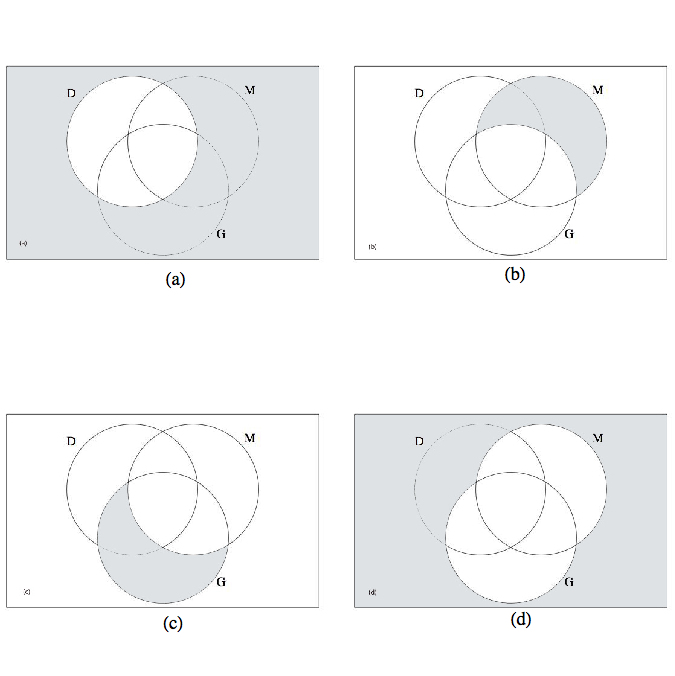
\includegraphics[width=1\linewidth]{images/fig-sol-1-2-7.png}
\caption*{\textbf{Figure 1.2.18:} }
\end{figure}
\end{divisionsolution}%
\begin{divisionsolution}{1.2.4.8}{}{exercise-14}%
\hypertarget{p-331}{}%
Let the sets \(D\), \(M\), \(G\), and \(U\) be as in exercise 7.  Let \(\lvert U \rvert  = 16,000\), \(\lvert D \rvert = 9,000\), \(|M|=
300\), and \(\lvert G \rvert = 1,000\). Also assume that the number of day students who are mathematics majors is 250, 50 of whom are graduate students, that there are 95 graduate mathematics majors, and that the total number of day graduate students is 700. Determine the number of students who are:\leavevmode%
\begin{multicols}{2}
\begin{enumerate}[label=(\alph*)]
\item\hypertarget{li-259}{}\hypertarget{p-332}{}%
evening students%
\item\hypertarget{li-260}{}\hypertarget{p-333}{}%
nonmathematics majors%
\item\hypertarget{li-261}{}\hypertarget{p-334}{}%
undergraduates (day or evening)%
\item\hypertarget{li-262}{}\hypertarget{p-335}{}%
day graduate nonmathematics majors%
\item\hypertarget{li-263}{}\hypertarget{p-336}{}%
evening graduate students%
\item\hypertarget{li-264}{}\hypertarget{p-337}{}%
evening graduate mathematics majors%
\item\hypertarget{li-265}{}\hypertarget{p-338}{}%
evening undergraduate nonmathematics majors%
\end{enumerate}
\end{multicols}
%
\end{divisionsolution}%
\section*{1.3 Cartesian Products and Power Sets}
\addcontentsline{toc}{section}{1.3 Cartesian Products and Power Sets}
\sectionmark{1.3 Cartesian Products and Power Sets}
\subsection*{1.3.4 EXERCISES FOR SECTION 1.3}
\addcontentsline{toc}{subsection}{1.3.4 EXERCISES FOR SECTION 1.3}
\begin{divisionsolution}{1.3.4.1}{}{exercise-15}%
\hypertarget{p-358}{}%
Let \(A = \{0, 2, 3\}\), \(B = \{2, 3\}\), \(C = \{1, 4\}\), and let the universal set be \(U = \{0, 1, 2, 3, 4\}\). List the elements of%
\par
\hypertarget{p-359}{}%
\leavevmode%
\begin{multicols}{2}
\begin{enumerate}[label=(\alph*)]
\item\hypertarget{li-271}{}\hypertarget{p-360}{}%
\(A \times B\)%
\item\hypertarget{li-272}{}\hypertarget{p-361}{}%
\(B \times  A\)%
\item\hypertarget{li-273}{}\hypertarget{p-362}{}%
\(A \times B\times C\)%
\item\hypertarget{li-274}{}\hypertarget{p-363}{}%
\(U \times \emptyset\)%
\item\hypertarget{li-275}{}\hypertarget{p-364}{}%
\(A \times  A^c\)%
\item\hypertarget{li-276}{}\hypertarget{p-365}{}%
\(B^2\)%
\item\hypertarget{li-277}{}\hypertarget{p-366}{}%
\(B^3\)%
\item\hypertarget{li-278}{}\hypertarget{p-367}{}%
\(B\times \mathcal{P}(B)\)%
\end{enumerate}
\end{multicols}
%
\par\smallskip%
\noindent\textbf{Answer}.\quad%
\hypertarget{p-368}{}%
\leavevmode%
\begin{enumerate}[label=(\alph*)]
\item\hypertarget{li-279}{}\(\{(0, 2), (0, 3), (2, 2), (2, 3), (3, 2), (3, 3)\}\)%
\item\hypertarget{li-280}{}\(\{(2, 0), (2, 2), (2, 3), (3, 0), (3, 2), (3, 3)\}\)%
\item\hypertarget{li-281}{}\(\{(0, 2, 1), (0, 2, 4), (0, 3, 1), (0, 3, 4), (2, 2, 1), (2, 2, 4),\\ (2, 3, 1), (2, 3, 4), (3, 2, 1), (3, 2, 4), (3, 3, 1), (3, 3, 4)\}\)%
\item\hypertarget{li-282}{}\(\emptyset\)%
\item\hypertarget{li-283}{}\(\{(0, 1), (0, 4), (2, 1), (2, 4), (3, 1), (3, 4)\}\)%
\item\hypertarget{li-284}{}\(\{(2, 2), (2, 3), (3, 2), (3, 3)\}\)%
\item\hypertarget{li-285}{}\(\{(2, 2, 2), (2, 2, 3), (2, 3, 2), (2, 3, 3), (3, 2, 2), (3, 2, 3), (3, 3, 2), (3, 3, 3)\}\)%
\item\hypertarget{li-286}{}\(\{(2, \emptyset ), (2, \{2\}), (2, \{3\}), (2, \{2, 3\}), (3, \emptyset ), (3, \{2\}), (3, \{3\}), (3, \{2, 3\})\}\)%
\end{enumerate}
%
\end{divisionsolution}%
\begin{divisionsolution}{1.3.4.2}{}{exercise-16}%
\hypertarget{p-369}{}%
Suppose that you are about to flip a coin and then roll a die. Let \(A = \{HEADS, TAILS\}\) and  \(B = \{1, 2, 3, 4, 5, 6\}\).%
\par
\hypertarget{p-370}{}%
\leavevmode%
\begin{enumerate}[label=(\alph*)]
\item\hypertarget{li-287}{}\hypertarget{p-371}{}%
What is \(|A \times  B|\)?%
\item\hypertarget{li-288}{}\hypertarget{p-372}{}%
How could you interpret the set \(A \times  B\) ?%
\end{enumerate}
%
\end{divisionsolution}%
\begin{divisionsolution}{1.3.4.3}{}{exercise-17}%
\hypertarget{p-373}{}%
List all two-element sets in \(\mathcal{P}(\{a,b,c,d\})\)%
\par\smallskip%
\noindent\textbf{Answer}.\quad%
\hypertarget{p-374}{}%
\(\{a, b\}, \{a, c\}, \{a, d\}, \{b, c\}, \{b, d\} \textrm{ and } \{c, d\}\)%
\end{divisionsolution}%
\begin{divisionsolution}{1.3.4.4}{}{exercise-18}%
\hypertarget{p-375}{}%
List all three-element sets in \(\mathcal{P}(\{a, b, c,d\})\).%
\end{divisionsolution}%
\begin{divisionsolution}{1.3.4.5}{}{exercise-19}%
\hypertarget{p-376}{}%
How many singleton (one-element) sets are there in \(\mathcal{P}(A)\) if \(\lvert A \rvert =n\) ?%
\par\smallskip%
\noindent\textbf{Answer}.\quad%
\hypertarget{p-377}{}%
There are \(n\) singleton subsets, one for each element.%
\end{divisionsolution}%
\begin{divisionsolution}{1.3.4.6}{}{exercise-20}%
\hypertarget{p-378}{}%
A person has four coins in his pocket: a penny, a nickel, a dime, and a quarter. How many different sums of money can he take out if he removes 3 coins at a time?%
\end{divisionsolution}%
\begin{divisionsolution}{1.3.4.7}{}{exercise-21}%
\hypertarget{p-379}{}%
Let \(A = \{+,-\}\) and \(B = \{00, 01, 10, 11\}\).%
\par
\hypertarget{p-380}{}%
\leavevmode%
\begin{enumerate}[label=(\alph*)]
\item\hypertarget{li-289}{}\hypertarget{p-381}{}%
List the elements of \(A \times  B\)%
\item\hypertarget{li-290}{}\hypertarget{p-382}{}%
How many elements do \(A ^4\) and \((A \times B)^3\) have?%
\end{enumerate}
%
\par\smallskip%
\noindent\textbf{Answer}.\quad%
\hypertarget{p-383}{}%
\leavevmode%
\begin{enumerate}[label=(\alph*)]
\item\hypertarget{li-291}{}\hypertarget{p-384}{}%
\(\{+00, +01, +10, +11, -00, -01, -10, -11\}\)%
\item\hypertarget{li-292}{}\hypertarget{p-385}{}%
\(16 \textrm{ and } 512\)%
\end{enumerate}
%
\end{divisionsolution}%
\begin{divisionsolution}{1.3.4.8}{}{exercise-22}%
\hypertarget{p-386}{}%
Let \(A = \{\bullet,\square ,\otimes \}\) and \(B = \{\square ,\ominus ,\bullet\}\).%
\par
\hypertarget{p-387}{}%
\leavevmode%
\begin{enumerate}[label=(\alph*)]
\item\hypertarget{li-293}{}\hypertarget{p-388}{}%
List the elements of \(A \times  B\) and \(B \times  A\). The parentheses and comma in an ordered pair are not necessary in cases such as this where the elements of each set are individual symbols.%
\item\hypertarget{li-294}{}\hypertarget{p-389}{}%
Identify the intersection of \(A \times  B\) and \(B \times  A\) for the case above, and then guess at a general rule for the intersection of \(A \times  B\) and \(B \times  A\), where \(A\) and \(B\) are any two sets.%
\end{enumerate}
%
\end{divisionsolution}%
\begin{divisionsolution}{1.3.4.9}{}{exercise-23}%
\hypertarget{p-390}{}%
Let \(A\) and \(B\) be nonempty sets. When are \(A \times  B\) and \(B \times  A\) equal?%
\par\smallskip%
\noindent\textbf{Answer}.\quad%
\hypertarget{p-391}{}%
They are equal when \(A=B\).%
\end{divisionsolution}%
\section*{1.4 Binary Representation of Positive Integers}
\addcontentsline{toc}{section}{1.4 Binary Representation of Positive Integers}
\sectionmark{1.4 Binary Representation of Positive Integers}
\subsection*{1.4.3 Exercises for Section 1.4}
\addcontentsline{toc}{subsection}{1.4.3 Exercises for Section 1.4}
\begin{divisionsolution}{1.4.3.1}{}{exercise-24}%
\hypertarget{p-428}{}%
Find the binary representation of each of the following positive integers by working through the algorithm by hand.  You can check your answer using the sage cell above.%
\par
\hypertarget{p-429}{}%
\leavevmode%
\begin{multicols}{2}
\begin{enumerate}[label=(\alph*)]
\item\hypertarget{li-314}{}\hypertarget{p-430}{}%
31%
\item\hypertarget{li-315}{}\hypertarget{p-431}{}%
32%
\item\hypertarget{li-316}{}\hypertarget{p-432}{}%
10%
\item\hypertarget{li-317}{}\hypertarget{p-433}{}%
100%
\end{enumerate}
\end{multicols}
%
\par\smallskip%
\noindent\textbf{Answer}.\quad%
\hypertarget{p-434}{}%
\leavevmode%
\begin{multicols}{2}
\begin{enumerate}[label=(\alph*)]
\item\hypertarget{li-318}{}\hypertarget{p-435}{}%
\(11111\)%
\item\hypertarget{li-319}{}\hypertarget{p-436}{}%
\(100000\)%
\item\hypertarget{li-320}{}\hypertarget{p-437}{}%
\(1010\)%
\item\hypertarget{li-321}{}\hypertarget{p-438}{}%
\(1100100\)%
\end{enumerate}
\end{multicols}
%
\end{divisionsolution}%
\begin{divisionsolution}{1.4.3.2}{}{exercise-25}%
\hypertarget{p-439}{}%
Find the binary representation of each of the following positive integers by working through the algorithm by hand.  You can check your answer using the sage cell above.%
\par
\hypertarget{p-440}{}%
\leavevmode%
\begin{multicols}{2}
\begin{enumerate}[label=(\alph*)]
\item\hypertarget{li-322}{}\hypertarget{p-441}{}%
64%
\item\hypertarget{li-323}{}\hypertarget{p-442}{}%
67%
\item\hypertarget{li-324}{}\hypertarget{p-443}{}%
28%
\item\hypertarget{li-325}{}\hypertarget{p-444}{}%
256%
\end{enumerate}
\end{multicols}
%
\end{divisionsolution}%
\begin{divisionsolution}{1.4.3.3}{}{exercise-26}%
\hypertarget{p-445}{}%
What positive integers have the following binary representations?%
\par
\hypertarget{p-446}{}%
\leavevmode%
\begin{multicols}{2}
\begin{enumerate}[label=(\alph*)]
\item\hypertarget{li-326}{}\hypertarget{p-447}{}%
10010%
\item\hypertarget{li-327}{}\hypertarget{p-448}{}%
10011%
\item\hypertarget{li-328}{}\hypertarget{p-449}{}%
101010%
\item\hypertarget{li-329}{}\hypertarget{p-450}{}%
10011110000%
\end{enumerate}
\end{multicols}
%
\par\smallskip%
\noindent\textbf{Answer}.\quad%
\hypertarget{p-451}{}%
\leavevmode%
\begin{multicols}{2}
\begin{enumerate}[label=(\alph*)]
\item\hypertarget{li-330}{}\hypertarget{p-452}{}%
\(18\)%
\item\hypertarget{li-331}{}\hypertarget{p-453}{}%
\(19\)%
\item\hypertarget{li-332}{}\hypertarget{p-454}{}%
\(42\)%
\item\hypertarget{li-333}{}\hypertarget{p-455}{}%
\(1264\)%
\end{enumerate}
\end{multicols}
%
\end{divisionsolution}%
\begin{divisionsolution}{1.4.3.4}{}{exercise-27}%
\hypertarget{p-456}{}%
What positive integers have the following binary representations?\leavevmode%
\begin{multicols}{2}
\begin{enumerate}[label=(\alph*)]
\item\hypertarget{li-334}{}\hypertarget{p-457}{}%
100001%
\item\hypertarget{li-335}{}\hypertarget{p-458}{}%
1001001%
\item\hypertarget{li-336}{}\hypertarget{p-459}{}%
1000000000%
\item\hypertarget{li-337}{}\hypertarget{p-460}{}%
1001110000%
\end{enumerate}
\end{multicols}
%
\end{divisionsolution}%
\begin{divisionsolution}{1.4.3.5}{}{exercise-28}%
\hypertarget{p-461}{}%
The number of bits in the binary representations of integers increases by one as the numbers double.  Using this fact, determine how many bits the binary representations of the following decimal numbers have without actually doing the full conversion.\leavevmode%
\begin{multicols}{4}
\begin{enumerate}[label=(\alph*)]
\item\hypertarget{li-338}{}\hypertarget{p-462}{}%
2017%
\item\hypertarget{li-339}{}\hypertarget{p-463}{}%
4000%
\item\hypertarget{li-340}{}\hypertarget{p-464}{}%
4500%
\item\hypertarget{li-341}{}\hypertarget{p-465}{}%
\(2^{50}\)%
\end{enumerate}
\end{multicols}
%
\par\smallskip%
\noindent\textbf{Answer}.\quad%
\hypertarget{p-466}{}%
There is a bit for each power of 2 up to the largest one needed to represent an integer, and you start counting with the zeroth power. For example, 2017 is between \(2^{10}=1024\) and \(2^{11}=2048\), and so the largest power needed is \(2^{10}\). Therefore there are \(11\) bits in binary 2017.%
\par
\hypertarget{p-467}{}%
\leavevmode%
\begin{multicols}{2}
\begin{enumerate}[label=(\alph*)]
\item\hypertarget{li-342}{}\hypertarget{p-468}{}%
\(11\)%
\item\hypertarget{li-343}{}\hypertarget{p-469}{}%
\(12\)%
\item\hypertarget{li-344}{}\hypertarget{p-470}{}%
\(13\)%
\item\hypertarget{li-345}{}\hypertarget{p-471}{}%
51%
\end{enumerate}
\end{multicols}
%
\end{divisionsolution}%
\begin{divisionsolution}{1.4.3.6}{}{exercise-29}%
\hypertarget{p-472}{}%
Let \(m\) be a positive integer with \(n\)-bit binary representation: \(a_{n-1}a_{n-2}\cdots  a_1a_0\) with \(a_{n-1}=1\) What are the smallest and largest values that \(m\) could have?%
\end{divisionsolution}%
\begin{divisionsolution}{1.4.3.7}{}{exercise-30}%
\hypertarget{p-473}{}%
If a positive integer is a multiple of 100, we can identify this fact from its decimal representation, since it will end with two zeros. What can you say about a positive integer if its binary representation ends with two zeros? What if it ends in \(k\) zeros?%
\par\smallskip%
\noindent\textbf{Answer}.\quad%
\hypertarget{p-474}{}%
A number must be a multiple of four if its binary representation ends in two zeros. If it ends in \(k\) zeros, it must be a multiple of \(2^k\).%
\end{divisionsolution}%
\begin{divisionsolution}{1.4.3.8}{}{exercise-31}%
\hypertarget{p-475}{}%
Can a multiple of ten be easily identified from its binary representation?%
\end{divisionsolution}%
\section*{1.5 Summation Notation and Generalizations}
\addcontentsline{toc}{section}{1.5 Summation Notation and Generalizations}
\sectionmark{1.5 Summation Notation and Generalizations}
\subsection*{1.5.3 Exercises for Section 1.5}
\addcontentsline{toc}{subsection}{1.5.3 Exercises for Section 1.5}
\begin{divisionsolution}{1.5.3.1}{}{exercise-32}%
\hypertarget{p-501}{}%
Calculate the following series:%
\par
\hypertarget{p-502}{}%
\leavevmode%
\begin{multicols}{2}
\begin{enumerate}[label=(\alph*)]
\item\hypertarget{li-359}{}\hypertarget{p-503}{}%
\(\sum_{i=1}^3 (2 + 3i)\)%
\item\hypertarget{li-360}{}\hypertarget{p-504}{}%
\(\sum_{i=-2}^1 i^2\)%
\item\hypertarget{li-361}{}\hypertarget{p-505}{}%
\(\sum_{j=0}^n 2^j\text{   }\) for \(n= 1, 2, 3, 4\)%
\item\hypertarget{li-362}{}\hypertarget{p-506}{}%
\(\sum_{k=1}^n (2k-1)\) for \(n = 1, 2, 3, 4\)%
\end{enumerate}
\end{multicols}
%
\par\smallskip%
\noindent\textbf{Answer}.\quad%
\hypertarget{p-507}{}%
\leavevmode%
\begin{multicols}{2}
\begin{enumerate}[label=(\alph*)]
\item\hypertarget{li-363}{}\hypertarget{p-508}{}%
\(24\)%
\item\hypertarget{li-364}{}\hypertarget{p-509}{}%
\(6\)%
\item\hypertarget{li-365}{}\hypertarget{p-510}{}%
\(3,7,15,31\)%
\item\hypertarget{li-366}{}\hypertarget{p-511}{}%
\(1,4,9,16\)%
\end{enumerate}
\end{multicols}
%
\end{divisionsolution}%
\begin{divisionsolution}{1.5.3.2}{}{exercise-33}%
\hypertarget{p-512}{}%
Calculate the following series:%
\par
\hypertarget{p-513}{}%
\leavevmode%
\begin{enumerate}[label=(\alph*)]
\item\hypertarget{li-367}{}\hypertarget{p-514}{}%
\(\sum_{k=1}^3 k^n\) for \(n = 1, 2, 3, 4\)%
\item\hypertarget{li-368}{}\hypertarget{p-515}{}%
\(\sum_{i=1}^5 20\)%
\item\hypertarget{li-369}{}\hypertarget{p-516}{}%
\(\sum_{j=0}^3 \left(n^j+1\right)\) for \(n = 1, 2, 3,4\)%
\item\hypertarget{li-370}{}\hypertarget{p-517}{}%
\(\sum_{k=-n}^n k\) for \(n = 1, 2, 3, 4\)%
\end{enumerate}
%
\end{divisionsolution}%
\begin{divisionsolution}{1.5.3.3}{}{exercise-34}%
\hypertarget{p-518}{}%
\leavevmode%
\begin{enumerate}[label=(\alph*)]
\item\hypertarget{li-371}{}\hypertarget{p-519}{}%
Express the formula \(\sum_{i=1}^n \frac{1}{i(i+1)}= \frac{n}{n+1}\)  without using summation notation.%
\item\hypertarget{li-372}{}\hypertarget{p-520}{}%
Verify this formula for \(n=3\).%
\item\hypertarget{li-373}{}\hypertarget{p-521}{}%
Repeat parts (a) and (b) for \(\sum_{i=1}^n i^3=\frac{n^2(n+1)^2}{4}\)%
\end{enumerate}
%
\par\smallskip%
\noindent\textbf{Answer}.\quad%
\hypertarget{p-522}{}%
\leavevmode%
\begin{enumerate}[label=(\alph*)]
\item\hypertarget{li-374}{}\hypertarget{p-523}{}%
\(\frac{1}{1 (1+1)}+\frac{1}{2 (2+1)}+\frac{1}{3 (3+1)}+\cdots +\frac{1}{n(n+1)}=\frac{n}{n+1}\)%
\item\hypertarget{li-375}{}\hypertarget{p-524}{}%
\(\frac{1}{1(2)}+\frac{1}{2(3)}+\frac{1}{3(4)}=\frac{1}{2}+\frac{1}{6}+\frac{1}{12}=\frac{3}{4}=\frac{3}{3+1}\)%
\item\hypertarget{li-376}{}\hypertarget{p-525}{}%
\(1+2^3+3^3+\cdots +n^3=\left(\frac{1}{4}\right)n^2(n+1)^2\) \(\quad 1+8+27=36 = \left(\frac{1}{4}\right)(3)^2(3+1)^2\)%
\end{enumerate}
%
\end{divisionsolution}%
\begin{divisionsolution}{1.5.3.4}{}{exercise-35}%
\hypertarget{p-526}{}%
Verify the following properties for \(n = 3\).%
\par
\hypertarget{p-527}{}%
\leavevmode%
\begin{enumerate}[label=(\alph*)]
\item\hypertarget{li-377}{}\hypertarget{p-528}{}%
\(\sum_{i=1}^n \left(a_i+ b_i\right) =\sum_{i=1}^n a_i +\sum_{i=1}^n  b_i\)%
\item\hypertarget{li-378}{}\hypertarget{p-529}{}%
\(c\left(\sum_{i=1}^n a_i\right) = \sum_{i=1}^n c a_i\)%
\end{enumerate}
%
\end{divisionsolution}%
\begin{divisionsolution}{1.5.3.5}{}{exercise-36}%
\hypertarget{p-530}{}%
Rewrite the following without summation sign for \(n = 3\). It is not necessary that you understand or expand the notation \(\left(
\begin{array}{c}
n \\
k \\
\end{array}
\right)\) at this point. \((x + y)^n= \sum_{k=0}^n \left(
\begin{array}{c}
n \\
k \\
\end{array}
\right)x^{n-k}y^k\).%
\par\smallskip%
\noindent\textbf{Answer}.\quad%
\hypertarget{p-531}{}%
\((x+y)^3=\left(\text{}_0^3\right)x^3+\left(\text{}_1^3\right)x^{2}y+\left.(_2^3\right)x y^2+\left(\text{}_3^3\right)y^n\)%
\end{divisionsolution}%
\begin{divisionsolution}{1.5.3.6}{}{exercise-37}%
\hypertarget{p-532}{}%
\leavevmode%
\begin{enumerate}[label=(\alph*)]
\item\hypertarget{li-379}{}\hypertarget{p-533}{}%
Draw the Venn diagram for \(\underset{i=1}{\overset{3}{\cap }}A_i\).%
\item\hypertarget{li-380}{}\hypertarget{p-534}{}%
Express in ``expanded format'': \(A\cup (\underset{i=1}{\overset{n}{\cap }}B_i)= \underset{i=1}{\overset{n}{\cap }}(A \cup B_n)\).%
\end{enumerate}
%
\end{divisionsolution}%
\begin{divisionsolution}{1.5.3.7}{}{exercise-38}%
\hypertarget{p-535}{}%
For any positive integer \(k\), let \(A_k = \{x \in \mathbb{Q}:k-1 < x \leq k\}\) and \(B_k = \{x \in \mathbb{Q}: -k < x < k\}\). What are the following sets?%
\par
\hypertarget{p-536}{}%
\leavevmode%
\begin{multicols}{2}
\begin{enumerate}[label=(\alph*)]
\item\hypertarget{li-381}{}\hypertarget{p-537}{}%
\(\underset{i=1}{\overset{5}{\cup }}A_i\)%
\item\hypertarget{li-382}{}\hypertarget{p-538}{}%
\(\underset{i=1}{\overset{5}{\cup }}B_i\)%
\item\hypertarget{li-383}{}\hypertarget{p-539}{}%
\(\underset{i=1}{\overset{5}{\cap }}A_i\)%
\item\hypertarget{li-384}{}\hypertarget{p-540}{}%
\(\underset{i=1}{\overset{5}{\cap }}B_i\)%
\end{enumerate}
\end{multicols}
%
\par\smallskip%
\noindent\textbf{Answer}.\quad%
\hypertarget{p-541}{}%
\leavevmode%
\begin{multicols}{2}
\begin{enumerate}[label=(\alph*)]
\item\hypertarget{li-385}{}\hypertarget{p-542}{}%
\(\{x\in \mathbb{Q}\mid 0 < x \leq 5\}\)%
\item\hypertarget{li-386}{}\hypertarget{p-543}{}%
\(\{x\in \mathbb{Q}\mid -5 < x < 5\}=B_5\)%
\item\hypertarget{li-387}{}\hypertarget{p-544}{}%
\(\emptyset\)%
\item\hypertarget{li-388}{}\hypertarget{p-545}{}%
\(\{x\in \mathbb{Q}\mid -1 < x < 1\}=B_1\)%
\end{enumerate}
\end{multicols}
%
\end{divisionsolution}%
\begin{divisionsolution}{1.5.3.8}{}{exercise-39}%
\hypertarget{p-546}{}%
For any positive integer \(k\), let \(A_k = \{x \in \mathbb{Q}:\text0 < x < 1/k\}\) and \(B _k = \{x \in \mathbb{Q}:\,0 < x < k\}\). What are the following sets?%
\par
\hypertarget{p-547}{}%
\leavevmode%
\begin{multicols}{2}
\begin{enumerate}[label=(\alph*)]
\item\hypertarget{li-389}{}\hypertarget{p-548}{}%
\(\underset{i=1}{\overset{\infty }{\cup }}A_i\)%
\item\hypertarget{li-390}{}\hypertarget{p-549}{}%
\(\underset{i=1}{\overset{\infty }{\cup }}B_i\)%
\item\hypertarget{li-391}{}\hypertarget{p-550}{}%
\(\underset{i=1}{\overset{\infty }{\cap }}A_i\)%
\item\hypertarget{li-392}{}\hypertarget{p-551}{}%
\(\underset{i=1}{\overset{\infty }{\cap }}B_i\)%
\end{enumerate}
\end{multicols}
%
\end{divisionsolution}%
\begin{divisionsolution}{1.5.3.9}{}{exercise-40}%
\hypertarget{p-552}{}%
The symbol \(\Pi\) is used for the product of numbers in the same way that \(\Sigma\) is used for sums. For example, \(\prod _{i=1}^5 x_i=x_1 x_2 x_3 x_4 x_5\). Evaluate the following:%
\par
\hypertarget{p-553}{}%
\leavevmode%
\begin{multicols}{2}
\begin{enumerate}[label=(\alph*)]
\item\hypertarget{li-393}{}\hypertarget{p-554}{}%
\(\prod _{i=1}^3 i^2\)%
\item\hypertarget{li-394}{}\hypertarget{p-555}{}%
\(\prod _{i=1}^3 (2i+1)\)%
\end{enumerate}
\end{multicols}
%
\par\smallskip%
\noindent\textbf{Answer}.\quad%
\hypertarget{p-556}{}%
\leavevmode%
\begin{multicols}{2}
\begin{enumerate}[label=(\alph*)]
\item\hypertarget{li-395}{}\hypertarget{p-557}{}%
\(36\)%
\item\hypertarget{li-396}{}\hypertarget{p-558}{}%
\(105\)%
\end{enumerate}
\end{multicols}
%
\end{divisionsolution}%
\begin{divisionsolution}{1.5.3.10}{}{exercise-41}%
\hypertarget{p-559}{}%
Evaluate%
\par
\hypertarget{p-560}{}%
\leavevmode%
\begin{multicols}{2}
\begin{enumerate}[label=(\alph*)]
\item\hypertarget{li-397}{}\hypertarget{p-561}{}%
\(\prod _{k=0}^3 2^k\)%
\item\hypertarget{li-398}{}\hypertarget{p-562}{}%
\(\prod _{k=1}^{100} \frac{k}{k+1}\)%
\end{enumerate}
\end{multicols}
%
\end{divisionsolution}%
\chapter*{2 Combinatorics}
\addcontentsline{toc}{chapter}{2 Combinatorics}
\chaptermark{2 Combinatorics}
\section*{2.1 Basic Counting Techniques - The Rule of Products}
\addcontentsline{toc}{section}{2.1 Basic Counting Techniques - The Rule of Products}
\sectionmark{2.1 Basic Counting Techniques - The Rule of Products}
\subsection*{2.1.3 Exercises}
\addcontentsline{toc}{subsection}{2.1.3 Exercises}
\begin{divisionsolution}{2.1.3.1}{}{exercise-42}%
\hypertarget{p-580}{}%
In horse racing, to bet the ``daily double'' is to select the winners of the first two races of the day. You win only if both selections are correct. In terms of the number of horses that are entered in the first two races, how many different daily double bets could be made?%
\par\smallskip%
\noindent\textbf{Answer}.\quad%
\hypertarget{p-581}{}%
If there are \(m\) horses in race 1 and \(n\) horses in race 2 then there are \(m \cdot n\) possible daily doubles.%
\end{divisionsolution}%
\begin{divisionsolution}{2.1.3.2}{}{exercise-shortcut}%
\hypertarget{p-582}{}%
Professor Shortcut records his grades using only his students' first and last initials. What is the smallest class size that will definitely force Prof. S. to use a different system?%
\end{divisionsolution}%
\begin{divisionsolution}{2.1.3.3}{}{exercise-44}%
\hypertarget{p-583}{}%
A certain shirt comes in four sizes and six colors. One also has the choice of a dragon, an alligator, or no emblem on the pocket. How many different shirts could you order?%
\par\smallskip%
\noindent\textbf{Answer}.\quad%
\hypertarget{p-584}{}%
\(72=4\cdot 6\cdot 3\)%
\end{divisionsolution}%
\begin{divisionsolution}{2.1.3.4}{}{exercise-45}%
\hypertarget{p-585}{}%
A builder of modular homes would like to impress his potential customers with the variety of styles of his houses. For each house there are blueprints for three different living rooms, four different bedroom configurations, and two different garage styles. In addition, the outside can be finished in cedar shingles or brick. How many different houses can be designed from these plans?%
\end{divisionsolution}%
\begin{divisionsolution}{2.1.3.5}{}{exercise-46}%
\hypertarget{p-586}{}%
The Pi Mu Epsilon mathematics honorary society of Outstanding University wishes to have a picture taken of its six officers. There will be two rows of three people. How many different way can the six officers be arranged?%
\par\smallskip%
\noindent\textbf{Answer}.\quad%
\hypertarget{p-587}{}%
\(720=6\cdot 5\cdot 4\cdot 3\cdot 2\cdot 1\)%
\end{divisionsolution}%
\begin{divisionsolution}{2.1.3.6}{}{exercise-47}%
\hypertarget{p-588}{}%
An automobile dealer has several options available for each of three different packages of a particular model car: a choice of two styles of seats in three different colors, a choice of four different radios, and five different exteriors. How many choices of automobile does a customer have?%
\end{divisionsolution}%
\begin{divisionsolution}{2.1.3.7}{}{exercise-48}%
\hypertarget{p-589}{}%
A clothing manufacturer has put out a mix-and-match collection consisting of two blouses, two pairs of pants, a skirt, and a blazer. How many outfits can you make? Did you consider that the blazer is optional? How many outfits can you make if the manufacturer adds a sweater to the collection?%
\par\smallskip%
\noindent\textbf{Answer}.\quad%
\hypertarget{p-590}{}%
If we always include the blazer in the outfit we would have 6 outfits. If we consider the blazer optional then there would be 12 outfits. When we add a sweater we have the same type of choice. Considering the sweater optional produces 24 outfits.%
\end{divisionsolution}%
\begin{divisionsolution}{2.1.3.8}{}{exercise-49}%
\hypertarget{p-591}{}%
As a freshman, suppose you had to take two of four lab science courses, one of two literature courses, two of three math courses, and one of seven physical education courses. Disregarding possible time conflicts, how many different schedules do you have to choose from?%
\end{divisionsolution}%
\begin{divisionsolution}{2.1.3.9}{}{exercise-50}%
\hypertarget{p-592}{}%
(a) Suppose each single character stored in a computer uses eight bits. Then each character is represented by a different sequence of eight 0's and 1's called a bit pattern. How many different bit patterns are there? (That is, how many different characters could be represented?)%
\par
\hypertarget{p-593}{}%
(b) How many bit patterns are palindromes (the same backwards as forwards)?%
\par
\hypertarget{p-594}{}%
(c) How many different bit patterns have an even number of 1's?%
\par\smallskip%
\noindent\textbf{Answer}.\quad%
\hypertarget{p-595}{}%
\leavevmode%
\begin{enumerate}[label=(\alph*)]
\item\hypertarget{li-399}{}\hypertarget{p-596}{}%
\(2^8=256\)%
\item\hypertarget{li-400}{}\hypertarget{p-597}{}%
\(2^4=16\). Here we are concerned only with the first four bits, since the last four must be the same.%
\item\hypertarget{li-401}{}\hypertarget{p-598}{}%
\(2^7=128\), you have no choice in the last bit.%
\end{enumerate}
%
\end{divisionsolution}%
\begin{divisionsolution}{2.1.3.10}{}{exercise-51}%
\hypertarget{p-599}{}%
Automobile license plates in Massachusetts usually consist of three digits followed by three letters. The first digit is never zero. How many different plates of this type could be made?%
\end{divisionsolution}%
\begin{divisionsolution}{2.1.3.11}{}{exercise-52}%
\hypertarget{p-600}{}%
(a) Let \(A = \{1, 2, 3, 4\}\). Determine the number of different subsets of \(A\).%
\par
\hypertarget{p-601}{}%
(b) Let \(A = \{1, 2, 3, 4, 5\}\). Determine the number of proper subsets of \(A\) .%
\par\smallskip%
\noindent\textbf{Answer}.\quad%
\hypertarget{p-602}{}%
\leavevmode%
\begin{multicols}{2}
\begin{enumerate}[label=(\alph*)]
\item\hypertarget{li-402}{}\hypertarget{p-603}{}%
\(16\)%
\item\hypertarget{li-403}{}\hypertarget{p-604}{}%
\(30\)%
\end{enumerate}
\end{multicols}
%
\end{divisionsolution}%
\begin{divisionsolution}{2.1.3.12}{}{exercise-53}%
\hypertarget{p-605}{}%
How many integers from 100 to 999 can be written in base ten without using the digit 7?%
\end{divisionsolution}%
\begin{divisionsolution}{2.1.3.13}{}{exercise-54}%
\hypertarget{p-606}{}%
Consider three persons, A, B, and C, who are to be seated in a row of three chairs. Suppose A and B are identical twins. How many seating arrangements of these persons can there be%
\par
\hypertarget{p-607}{}%
\leavevmode%
\begin{multicols}{2}
\begin{enumerate}[label=(\alph*)]
\item\hypertarget{li-404}{}\hypertarget{p-608}{}%
If you are a total stranger?%
\item\hypertarget{li-405}{}\hypertarget{p-609}{}%
If you are A and B's mother?%
\end{enumerate}
\end{multicols}
%
\par
\hypertarget{p-610}{}%
This problem is designed to show you that different people can have different correct answers to the same problem.%
\par\smallskip%
\noindent\textbf{Answer}.\quad%
\hypertarget{p-611}{}%
\leavevmode%
\begin{multicols}{2}
\begin{enumerate}[label=(\alph*)]
\item\hypertarget{li-406}{}\hypertarget{p-612}{}%
\(3\)%
\item\hypertarget{li-407}{}\hypertarget{p-613}{}%
\(6\)%
\end{enumerate}
\end{multicols}
%
\end{divisionsolution}%
\begin{divisionsolution}{2.1.3.14}{}{exercise-55}%
\hypertarget{p-614}{}%
How many ways can a student do a ten-question true-false exam if he or she can choose not to answer any number of questions?%
\end{divisionsolution}%
\begin{divisionsolution}{2.1.3.15}{}{exercise-56}%
\hypertarget{p-615}{}%
Suppose you have a choice of fish, lamb, or beef for a main course, a choice of peas or carrots for a vegetable, and a choice of pie, cake, or ice cream for dessert. If you must order one item from each category, how many different dinners are possible?%
\par\smallskip%
\noindent\textbf{Answer}.\quad%
\hypertarget{p-616}{}%
\(18\)%
\end{divisionsolution}%
\begin{divisionsolution}{2.1.3.16}{}{exercise-57}%
\hypertarget{p-617}{}%
Suppose you have a choice of vanilla, chocolate, or strawberry for ice cream, a choice of peanuts or walnuts for chopped nuts, and a choice of hot fudge or marshmallow for topping. If you must order one item from each category, how many different sundaes are possible?%
\end{divisionsolution}%
\begin{divisionsolution}{2.1.3.17}{}{exercise-58}%
\hypertarget{p-618}{}%
A questionnaire contains six questions each having yes-no answers. For each yes response, there is a follow-up question with four possible responses.%
\par
\hypertarget{p-619}{}%
\leavevmode%
\begin{enumerate}[label=(\alph*)]
\item\hypertarget{li-408}{}\hypertarget{p-620}{}%
Draw a tree diagram that illustrates how many ways a single question in the questionnaire can be answered.%
\item\hypertarget{li-409}{}\hypertarget{p-621}{}%
How many ways can the questionnaire be answered?%
\end{enumerate}
%
\par\smallskip%
\noindent\textbf{Answer}.\quad%
\leavevmode%
\begin{figure}
\centering
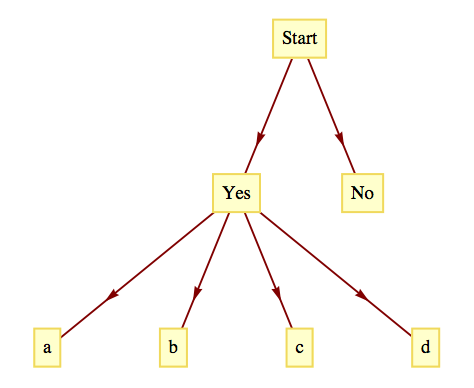
\includegraphics[width=1\linewidth]{images/fig-sol-2-1-17.png}
\caption*{\textbf{Figure 2.1.8:} Solution to 17(a)}
\end{figure}
\hypertarget{p-622}{}%
\leavevmode%
\begin{enumerate}[label=(\alph*)]
\item\hypertarget{li-410}{}\hypertarget{p-623}{}%
See Figure~2.1.8%
\item\hypertarget{li-411}{}\hypertarget{p-624}{}%
\(5^6\)%
\end{enumerate}
%
\end{divisionsolution}%
\begin{divisionsolution}{2.1.3.18}{}{exercise-59}%
\hypertarget{p-625}{}%
Ten people are invited to a dinner party. How many ways are there of seating them at a round table? If the ten people consist of five men and five women, how many ways are there of seating them if each man must be surrounded by two women around the table?%
\end{divisionsolution}%
\begin{divisionsolution}{2.1.3.19}{}{exercise-60}%
\hypertarget{p-626}{}%
How many ways can you separate a set with \(n\)  elements into two nonempty subsets if the order of the subsets is immaterial? What if the order of the subsets is important?%
\par\smallskip%
\noindent\textbf{Answer}.\quad%
\hypertarget{p-627}{}%
\(2^{n-1}-1\) and \(2^n-2\)%
\end{divisionsolution}%
\begin{divisionsolution}{2.1.3.20}{}{exercise-61}%
\hypertarget{p-628}{}%
A gardener has three flowering shrubs and four nonflowering shrubs, where all shrubs are distinguishable from one another. He must plant these shrubs in a row using an alternating pattern, that is, a shrub must be of a different type from that on either side. How many ways can he plant these shrubs? If he has to plant these shrubs in a circle using the same pattern, how many ways can he plant this circle? Note that one nonflowering shrub will be left out at the end.%
\end{divisionsolution}%
\section*{2.2 Permutations}
\addcontentsline{toc}{section}{2.2 Permutations}
\sectionmark{2.2 Permutations}
\subsection*{2.2.2 Exercises}
\addcontentsline{toc}{subsection}{2.2.2 Exercises}
\begin{divisionsolution}{2.2.2.1}{}{exercise-62}%
\hypertarget{p-665}{}%
If a raffle has three different prizes and there are 1,000 raffle tickets sold, how many different ways can the prizes be distributed?%
\par\smallskip%
\noindent\textbf{Answer}.\quad%
\hypertarget{p-666}{}%
\(P(1000,3)\)%
\end{divisionsolution}%
\begin{divisionsolution}{2.2.2.2}{}{exercise-63}%
\hypertarget{p-667}{}%
\leavevmode%
\begin{enumerate}[label=(\alph*)]
\item\hypertarget{li-421}{}How many three-digit numbers can be formed from the digits 1, 2, 3 if no repetition of digits is allowed? List the three-digit numbers.%
\item\hypertarget{li-422}{}How many two-digit numbers can be formed if no repetition of digits is allowed? List them.%
\item\hypertarget{li-423}{}How many two-digit numbers can be obtained if repetition is allowed?%
\end{enumerate}
%
\end{divisionsolution}%
\begin{divisionsolution}{2.2.2.3}{}{exercise-64}%
\hypertarget{p-668}{}%
How many eight-letter words can be formed from the 26 letters in the alphabet? Even without concerning ourselves about whether the words make sense, there are two interpretations of this problem. Answer both.%
\par\smallskip%
\noindent\textbf{Answer}.\quad%
\hypertarget{p-669}{}%
With repetition: \(26^8\approx  2.0883\times 10^{11}\)%
\par
\hypertarget{p-670}{}%
Without repetition: \(P(26,8) \approx 6.2991\ 10^{10}\)%
\end{divisionsolution}%
\begin{divisionsolution}{2.2.2.4}{}{exercise-65}%
\hypertarget{p-671}{}%
Let \(A\) be a set with \(\lvert A \rvert = n \). Determine%
\par
\hypertarget{p-672}{}%
\leavevmode%
\begin{enumerate}[label=(\alph*)]
\item\hypertarget{li-424}{}\hypertarget{p-673}{}%
\(\lvert A^3 \rvert \)%
\item\hypertarget{li-425}{}\hypertarget{p-674}{}%
\(\lvert \{ (a, b, c) \mid a, b, c \in A \textrm{ and each coordinate is different}\} \rvert \)%
\end{enumerate}
%
\end{divisionsolution}%
\begin{divisionsolution}{2.2.2.5}{}{exercise-66}%
\hypertarget{p-675}{}%
The state finals of a high school track meet involves fifteen schools. How many ways can these schools be listed in the program?%
\par\smallskip%
\noindent\textbf{Answer}.\quad%
\hypertarget{p-676}{}%
\(15!\)%
\end{divisionsolution}%
\begin{divisionsolution}{2.2.2.6}{}{exercise-67}%
\hypertarget{p-677}{}%
Consider the three-digit numbers that can be formed from the digits 1, 2, 3, 4, and 5 with no repetition of digits allowed.%
\par
\hypertarget{p-678}{}%
a. How many of these are even numbers?%
\par
\hypertarget{p-679}{}%
b. How many are greater than 250?%
\end{divisionsolution}%
\begin{divisionsolution}{2.2.2.7}{}{exercise-68}%
\hypertarget{p-680}{}%
All 15 players on the Tall U. basketball team are capable of playing any position.\leavevmode%
\begin{enumerate}[label=(\alph*)]
\item\hypertarget{li-426}{}\hypertarget{p-681}{}%
How many ways can the coach at Tall U. fill the five starting positions in a game?%
\item\hypertarget{li-427}{}\hypertarget{p-682}{}%
What is the answer if the center must be one of two players?%
\end{enumerate}
%
\par\smallskip%
\noindent\textbf{Answer}.\quad%
\hypertarget{p-683}{}%
\leavevmode%
\begin{enumerate}[label=(\alph*)]
\item\hypertarget{li-428}{}\(P(15,5)=360360\)%
\item\hypertarget{li-429}{}\(2\cdot 14\cdot 13\cdot 12\cdot 11=48048\)%
\end{enumerate}
%
\end{divisionsolution}%
\begin{divisionsolution}{2.2.2.8}{}{exercise-69}%
\hypertarget{p-684}{}%
\leavevmode%
\begin{enumerate}[label=(\alph*)]
\item\hypertarget{li-430}{}\hypertarget{p-685}{}%
How many ways can a gardener plant five different species of shrubs in a circle?%
\item\hypertarget{li-431}{}\hypertarget{p-686}{}%
What is the answer if two of the shrubs are the same?%
\item\hypertarget{li-432}{}\hypertarget{p-687}{}%
What is the answer if all the shrubs are identical?%
\end{enumerate}
%
\end{divisionsolution}%
\begin{divisionsolution}{2.2.2.9}{}{exercise-70}%
\hypertarget{p-688}{}%
The president of the Math and Computer Club would like to arrange a meeting with six attendees, the president included. There will be three computer science majors and three math majors at the meeting. How many ways can the six people be seated at a circular table if the president does not want people with the same majors to sit next to one other?%
\par\smallskip%
\noindent\textbf{Answer}.\quad%
\hypertarget{p-689}{}%
\(2\cdot P(3,3)=12\)%
\end{divisionsolution}%
\begin{divisionsolution}{2.2.2.10}{}{exercise-71}%
\hypertarget{p-690}{}%
Six people apply for three identical jobs and all are qualified for the positions. Two will work in New York and the other one will work in San Diego. How many ways can the positions be filled?%
\end{divisionsolution}%
\begin{divisionsolution}{2.2.2.11}{}{exercise-72}%
\hypertarget{p-691}{}%
Let \(A = \{1, 2, 3, 4\} \). Determine the cardinality of%
\par
\hypertarget{p-692}{}%
\leavevmode%
\begin{enumerate}[label=(\alph*)]
\item\hypertarget{li-433}{}\hypertarget{p-693}{}%
\(\{ (a_1,a_2) \mid a_1 \neq a_2 \}\)%
\item\hypertarget{li-434}{}\hypertarget{p-694}{}%
What is the answer to the previous part if \(\lvert A \rvert = n\)%
\item\hypertarget{li-435}{}\hypertarget{p-695}{}%
If \(\lvert A \rvert =n\), determine the number of \(m\)-tuples in \(A\), \(m \leq n\), where each coordinate is different from the other coordinates.%
\end{enumerate}
%
\par\smallskip%
\noindent\textbf{Answer}.\quad%
\hypertarget{p-696}{}%
\leavevmode%
\begin{enumerate}[label=(\alph*)]
\item\hypertarget{li-436}{}\(P(4,2)=12\)%
\item\hypertarget{li-437}{}\hypertarget{p-697}{}%
\(P(n;2)=n(n-1)\)%
\item\hypertarget{li-438}{}\hypertarget{p-698}{}%
Case 1: \(m>n\). Since the coordinates must be different, this case is impossible.%
\par
\hypertarget{p-699}{}%
Case 2: \(m\leqslant n. P(n;m)\).%
\end{enumerate}
%
\end{divisionsolution}%
\section*{2.3 Partitions of Sets and the Law of Addition}
\addcontentsline{toc}{section}{2.3 Partitions of Sets and the Law of Addition}
\sectionmark{2.3 Partitions of Sets and the Law of Addition}
\subsection*{2.3.3 Exercises for Section 2.3}
\addcontentsline{toc}{subsection}{2.3.3 Exercises for Section 2.3}
\begin{divisionsolution}{2.3.3.1}{}{exercise-73}%
\hypertarget{p-739}{}%
List all partitions of the set \(A =\{a, b, c\}\).%
\par\smallskip%
\noindent\textbf{Answer}.\quad%
\hypertarget{p-740}{}%
\(\{\{a\}, \{b\}, \{c\}\}, \{\{a, b\}, \{c\}\}, \{\{a, c\}, \{b\}\}, \{\{a\}, \{b, c\}\}, \{\{a, b, c\}\}\)%
\end{divisionsolution}%
\begin{divisionsolution}{2.3.3.2}{}{exercise-74}%
\hypertarget{p-741}{}%
Which of the following collections of subsets of the plane, \(\mathbb{R}^2\), are partitions?%
\par
\hypertarget{p-742}{}%
\leavevmode%
\begin{enumerate}[label=(\alph*)]
\item\hypertarget{li-448}{}\hypertarget{p-743}{}%
\(\{ \{(x, y) \mid x + y = c \} \mid c \in \mathbb{R} \}\)%
\item\hypertarget{li-449}{}\hypertarget{p-744}{}%
The set of all circles in \(\mathbb{R}^2 \)%
\item\hypertarget{li-450}{}\hypertarget{p-745}{}%
The set of all circles in \(\mathbb{R}^2\) centered at the origin together with the set \(\{(0,0)\}\)%
\item\hypertarget{li-451}{}\hypertarget{p-746}{}%
\(\{\{(x, y)\} \mid (x, y) \in \mathbb{R}^2  \} \)%
\end{enumerate}
%
\end{divisionsolution}%
\begin{divisionsolution}{2.3.3.3}{}{exercise-75}%
\hypertarget{p-747}{}%
A student, on an exam paper, defined the term partition the following way: ``Let \(A\)  be a set. A partition of \(A\) is any set of nonempty subsets \(A_1, A_2, A_3, \dots\)  of \(A\) such that each element of \(A\) is in one of the subsets.''  Is this definition correct? Why?%
\par\smallskip%
\noindent\textbf{Answer}.\quad%
\hypertarget{p-748}{}%
No. By this definition it is possible that an element of \(A\) might belong to two of the subsets.%
\end{divisionsolution}%
\begin{divisionsolution}{2.3.3.4}{}{exercise-76}%
\hypertarget{p-749}{}%
Let \(A_1\) and \(A_2\) be subsets of a set \(U\).   Draw a Venn diagram of this situation and shade in the subsets \(A_1 \cap A_2\), \(A_1^c \cap A_2\), \(A_1 \cap A_2^c\), and \(A_1^c \cap A_2^c\) . Use the resulting diagram and the definition of partition to convince yourself that the subset of these four subsets that are nonempty form a partition of \(U\).%
\end{divisionsolution}%
\begin{divisionsolution}{2.3.3.5}{}{exercise-77}%
\hypertarget{p-750}{}%
Show that \(\{\{2 n \mid n \in \mathbb{Z}\}, \{2 n + 1 \mid n \in \mathbb{Z}\}\}\) is a partition of \(\mathbb{Z}\). Describe this partition using only words.%
\par\smallskip%
\noindent\textbf{Answer}.\quad%
\hypertarget{p-751}{}%
The first subset is all the even integers and the second is all the odd integers. These two sets do not intersect and they cover the integers completely.%
\end{divisionsolution}%
\begin{divisionsolution}{2.3.3.6}{}{exercise-78}%
\hypertarget{p-752}{}%
\leavevmode%
\begin{enumerate}[label=(\alph*)]
\item\hypertarget{li-452}{}\hypertarget{p-753}{}%
A group of 30 students were surveyed and it was found that 18 of them took Calculus and 12 took Physics. If all students took at least one course, how many took both Calculus and Physics? Illustrate using a Venn diagram.%
\item\hypertarget{li-453}{}\hypertarget{p-754}{}%
What is the answer to the question in part (a) if five students did not take either of the two courses? Illustrate using a Venn diagram.%
\end{enumerate}
%
\end{divisionsolution}%
\begin{divisionsolution}{2.3.3.7}{}{exercise-79}%
\hypertarget{p-755}{}%
A survey of 90 people, 47 of them played tennis and 42 of them swam. If 17 of them participated in both activities, how many of them participated in neither?%
\par\smallskip%
\noindent\textbf{Answer}.\quad%
\hypertarget{p-756}{}%
Since 17 participated in both activities, 30 of the tennis players only played tennis and 25 of the swimmers only swam. Therefore, \(17+30+25=72\) of those who were surveyed participated in an activity and so 18 did not.%
\end{divisionsolution}%
\begin{divisionsolution}{2.3.3.8}{}{exercise-80}%
\hypertarget{p-757}{}%
A survey of 300 people found that 60 owned an iPhone, 75 owned a Blackberry, and 30 owned an Android phone. Furthermore, 40 owned both an iPhone and a Blackberry, 12 owned both an iPhone and an Android phone, and 8 owned a Blackberry and an Android phone. Finally, 3 owned all three phones.%
\par
\hypertarget{p-758}{}%
\leavevmode%
\begin{enumerate}[label=(\alph*)]
\item\hypertarget{li-454}{}\hypertarget{p-759}{}%
How many people surveyed owned none of the three phones?%
\item\hypertarget{li-455}{}\hypertarget{p-760}{}%
How many people owned a Blackberry but not an iPhone?%
\item\hypertarget{li-456}{}\hypertarget{p-761}{}%
How many owned a Blackberry but not an Android?%
\end{enumerate}
%
\end{divisionsolution}%
\begin{divisionsolution}{2.3.3.9}{}{exercise-81}%
\hypertarget{p-762}{}%
Regarding the Theorem~2.3.9,\leavevmode%
\begin{enumerate}[label=(\alph*)]
\item\hypertarget{li-457}{}\hypertarget{p-763}{}%
Use the two set inclusion-exclusion law  to derive the  three set inclusion-exclusion law. Note: A knowledge of basic set laws is needed for this exercise.%
\item\hypertarget{li-458}{}\hypertarget{p-764}{}%
State and derive the inclusion-exclusion law for four sets.%
\end{enumerate}
%
\par\smallskip%
\noindent\textbf{Solution}.\quad%
\hypertarget{p-765}{}%
We assume that \(\lvert A_1 \cup A_2 \rvert = \lvert A_1 \rvert +\lvert  A_2\rvert  -\lvert A_1\cap A_2\rvert   \).%
\begin{equation*}
\begin{split}
\lvert A_1 \cup A_2\cup A_3 \rvert  &  =\lvert (A_1\cup A_2) \cup A_3 \rvert   \quad  Why?\\
& = \lvert A_1\cup A_2\rvert   +\lvert  A_3 \rvert  -\lvert (A_1\cup A_2)\cap A_3\rvert \quad Why? \\
& =\lvert (A_1\cup A_2\rvert   +\lvert  A_3\rvert  -\lvert (A_1\cap A_3)\cup (A_2\cap A_3)\rvert \quad Why?\\
& =\lvert  A_1\rvert  +\lvert  A_2\rvert  -\lvert A_1\cap A_2\rvert   +\lvert  A_3\rvert \\
& \quad -(\lvert A_1\cap A_3\rvert   +\lvert A_2\cap A_3\rvert   -\lvert (A_1\cap A_3)\cap (A_2\cap A_3)\rvert\quad Why?\\
& =\lvert  A_1\rvert  +\lvert  A_2\rvert  +\lvert  A_3\rvert  -\lvert A_1\cap A_2\rvert -\lvert A_1\cap A_3\rvert\\
& \quad  -\lvert A_2\cap A_3\rvert +\lvert A_1\cap A_2\cap A_3\rvert \quad Why?  
\end{split}
\end{equation*}
%
\par
\hypertarget{p-766}{}%
The law for four sets is%
\begin{equation*}
\begin{split}
\lvert A_1\cup A_2\cup A_3\cup A_4\rvert  & =\lvert  A_1\rvert  +\lvert  A_2\rvert  +\lvert  A_3\rvert  +\lvert  A_4\rvert\\
& \quad  -\lvert A_1\cap A_2\rvert  -\lvert A_1\cap A_3\rvert  -\lvert A_1\cap A_4\rvert \\
& \quad \quad -\lvert A_2\cap A_3\rvert   -\lvert A_2\cap A_4\rvert -\lvert A_3\cap A_4\rvert   \\
& \quad +\lvert A_1\cap A_2\cap A_3\rvert +\lvert A_1\cap A_2\cap A_4\rvert   \\
& \quad \quad +\lvert A_1\cap A_3\cap A_4\rvert +\lvert A_2\cap A_3\cap A_4\rvert \\
& \quad   -\lvert A_1\cap A_2\cap A_3\cap A_4\rvert  
\end{split}
\end{equation*}
%
\par
\hypertarget{p-767}{}%
Derivation:%
\begin{equation*}
\begin{split}
\lvert A_1\cup A_2\cup A_3\cup A_4\rvert & = \lvert (A_1\cup A_2\cup A_3)\cup A_4\rvert  \\
& = \lvert  (A_1\cup A_2\cup A_3\rvert   +\lvert  A_4\rvert  -\lvert (A_1\cup A_2\cup A_3)\cap A_4\rvert\\
& = \lvert  (A_1\cup A_2\cup A_3\rvert   +\lvert  A_4\rvert \\
& \quad -\lvert (A_1\cap A_4)\cup (A_2\cap A_4)\cup (A_3\cap A_4)\rvert  \\
& = \lvert  A_1\rvert  +\lvert  A_2\rvert  +\lvert  A_3\rvert  -\lvert A_1\cap A_2\rvert  -\lvert A_1\cap A_3\rvert  \\
& \quad -\lvert A_2\cap A_3\rvert   +\lvert A_1\cap A_2\cap A_3\rvert   +\lvert  A_4\rvert  -\lvert A_1\cap A_4\rvert    \\
& \quad+\lvert A_2\cap A_4\rvert   +\lvert A_3\cap A_4\rvert  -\lvert (A_1\cap A_4)\cap (A_2\cap A_4)\rvert  \\
& \quad  -\lvert (A_1\cap A_4)\cap (A_3\cap A_4)\rvert   -\lvert (A_2\cap A_4)\cap (A_3\cap A_4)\rvert \\
& \quad  +\lvert (A_1\cap A_4)\cap (A_2\cap A_4)\cap (A_3\cap A_4)\rvert  \\
& =\lvert  A_1\rvert  +\lvert  A_2\rvert  +\lvert  A_3\rvert  +\lvert  A_4\rvert  -\lvert A_1\cap A_2\rvert   -\lvert A_1\cap A_3\rvert   \\
& \quad  -\lvert A_2\cap A_3\rvert   -\lvert A_1\cap A_4\rvert   -\lvert A_2\cap A_4\rvert  \quad  -\lvert A_3\cap A_4\rvert  \\
& \quad  +\lvert A_1\cap A_2\cap A_3\rvert  +\lvert A_1\cap A_2\cap A_4\rvert  \\
& \quad  +\lvert A_1\cap A_3\cap A_4\rvert  +\lvert A_2\cap A_3\cap A_4\rvert \\
& \quad     -\lvert A_1\cap A_2 \cap A_3\cap A_4\rvert 
\end{split}   
\end{equation*}
%
\end{divisionsolution}%
\begin{divisionsolution}{2.3.3.10}{}{exercise-82}%
\hypertarget{p-768}{}%
To complete your spring schedule, you must add Calculus and Physics. At 9:30, there are three Calculus sections and two Physics sections; while at 11:30, there are two Calculus sections and three Physics sections.  How many ways can you complete your schedule if your only open periods are 9:30 and 11:30?%
\end{divisionsolution}%
\begin{divisionsolution}{2.3.3.11}{}{exercise-83}%
\hypertarget{p-769}{}%
The definition of \(\mathbb{Q}  = \{a/b \mid a, b \in \mathbb{Z}, b \neq 0\}\) given in Chapter 1 is  awkward. If we use the definition to list elements in \(\mathbb{Q}\), we will have duplications such as \(\frac{1}{2}\), \(\frac{-2}{-4}\) and \(\frac{300}{600}\)   Try to write a more precise definition of the rational numbers so that there is no duplication of elements.%
\par\smallskip%
\noindent\textbf{Answer}.\quad%
\hypertarget{p-770}{}%
Partition the set of fractions into blocks, where each block contains fractions that are numerically equivalent. Describe how you would determine whether two fractions belong to the same block. Redefine the rational numbers to be this partition. Each rational number is a set of fractions.%
\end{divisionsolution}%
\section*{2.4 Combinations and the Binomial Theorem}
\addcontentsline{toc}{section}{2.4 Combinations and the Binomial Theorem}
\sectionmark{2.4 Combinations and the Binomial Theorem}
\subsection*{2.4.4 Exercises}
\addcontentsline{toc}{subsection}{2.4.4 Exercises}
\begin{divisionsolution}{2.4.4.1}{}{exercise-84}%
\hypertarget{p-806}{}%
The judiciary committee at a college is made up of three faculty members and four students. If ten faculty members and 25 students have been nominated for the committee, how many judiciary committees could be formed at this point?%
\par\smallskip%
\noindent\textbf{Answer}.\quad%
\hypertarget{p-807}{}%
\(\binom{10}{3}\cdot \binom{25}{4}=1,518,000\)%
\end{divisionsolution}%
\begin{divisionsolution}{2.4.4.2}{}{exercise-85}%
\hypertarget{p-808}{}%
Suppose that a single character is stored in a computer using eight bits.%
\par
\hypertarget{p-809}{}%
a. How many bit patterns have exactly three 1's?%
\par
\hypertarget{p-810}{}%
b. How many bit patterns have at least two 1's?%
\par\smallskip%
\noindent\textbf{Hint}.\quad%
\hypertarget{p-811}{}%
Think of the set of positions that contain a 1 to turn this is into a question about sets.%
\par\smallskip%
\noindent\textbf{Solution}.\quad%
\hypertarget{p-812}{}%
(a) \(\binom{8}{3}\) (b) \(2^8-(\binom{8}{0}+\binom{8}{1})\)%
\end{divisionsolution}%
\begin{divisionsolution}{2.4.4.3}{}{exercise-86}%
\hypertarget{p-813}{}%
How many subsets of \(\{1, 2, 3, \dots , 10\}\) contain at least seven elements?%
\par\smallskip%
\noindent\textbf{Answer}.\quad%
\hypertarget{p-814}{}%
\(\binom{10}{7} +\binom{10}{8} +\binom{10}{9} +\binom{10}{10}= 120+45+10+1=176 \)%
\end{divisionsolution}%
\begin{divisionsolution}{2.4.4.4}{}{exercise-87}%
\hypertarget{p-815}{}%
The congressional committees on mathematics and computer science are made up of five representatives each, and a congressional rule is that the two committees must be disjoint. If there are 385 members of congress, how many ways could the committees be selected?%
\end{divisionsolution}%
\begin{divisionsolution}{2.4.4.5}{}{exercise-88}%
\hypertarget{p-816}{}%
\index{Lattice Paths}The image below shows a 6 by 6 grid and an example of a \terminology{lattice path} that could be taken from \((0,0)\)  to \((6,6)\), which is a path taken by traveling along grid lines going only to the right and up. How many different lattice paths are there of this type?  Generalize to the case of lattice paths from \((0,0)\) to \((m,n)\)  for any nonnegative integers \(m\) and \(n\).%
\begin{figure}
\centering
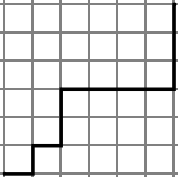
\includegraphics[width=0.5\linewidth]{images/fig-lattice-path-6.png}
\caption*{\textbf{Figure 2.4.12:} A lattice path}
\end{figure}
\par\smallskip%
\noindent\textbf{Hint}.\quad%
\hypertarget{p-817}{}%
Think of each path as a sequence of instructions to go right (R) and up (U).%
\par\smallskip%
\noindent\textbf{Answer}.\quad%
\hypertarget{p-818}{}%
Each path can be described as a sequence or R's and U's with exactly six of each.   The six positions in which R's could be placed can be selected from the twelve positions in the sequence \(\binom{12}{6}\) ways.  We can generalize this logic and see that there are \(\binom{m+n}{m}\) paths from \((0,0)\) to \((m,n)\).%
\end{divisionsolution}%
\begin{divisionsolution}{2.4.4.6}{}{exercise-89}%
\hypertarget{p-819}{}%
How many of the lattice paths from \((0,0)\) to \((6,6)\) pass through \((3,3)\) as the one in Figure~12 does?%
\end{divisionsolution}%
\begin{divisionsolution}{2.4.4.7}{}{exercise-90}%
\hypertarget{p-820}{}%
A poker game is played with 52 cards.  At the start of a game, each player gets five of the cards.  The order in which cards are dealt doesn't matter.\leavevmode%
\begin{enumerate}[label=(\alph*)]
\item\hypertarget{li-463}{}\hypertarget{p-821}{}%
How many ``hands'' of five cards are possible?%
\item\hypertarget{li-464}{}\hypertarget{p-822}{}%
If there are four people playing, how many initial five-card ``hands'' are possible, taking into account all players and their positions at the table?  Position with respect to the dealer does matter.%
\end{enumerate}
%
\par\smallskip%
\noindent\textbf{Answer}.\quad%
\hypertarget{p-823}{}%
\leavevmode%
\begin{enumerate}[label=(\alph*)]
\item\hypertarget{li-465}{}\hypertarget{p-824}{}%
\(C(52,5)=2,598,960\)%
\item\hypertarget{li-466}{}\hypertarget{p-825}{}%
\(\binom{52}{5}\cdot \binom{47}{5}\cdot \binom{42}{5}\cdot \binom{37}{5}\)%
\end{enumerate}
%
\end{divisionsolution}%
\begin{divisionsolution}{2.4.4.8}{}{exercise-91}%
\hypertarget{p-826}{}%
A flush in a five-card poker hand is five cards of the same suit. The suits are spades, clubs, diamonds and hearts.  How many spade flushes are possible in a 52-card deck? How many flushes are possible in any suit?%
\end{divisionsolution}%
\begin{divisionsolution}{2.4.4.9}{}{exercise-92}%
\hypertarget{p-827}{}%
How many five-card poker hands using 52 cards contain exactly two aces?%
\par\smallskip%
\noindent\textbf{Answer}.\quad%
\hypertarget{p-828}{}%
\(\binom{4}{2} \cdot \binom{48}{3} = 6 \cdot 17296=103776\)%
\end{divisionsolution}%
\begin{divisionsolution}{2.4.4.10}{}{exercise-93}%
\hypertarget{p-829}{}%
In poker, a full house is three-of-a-kind and a pair in one hand; for example, three fives and two queens. How many full houses are possible from a 52-card deck?  You can use the sage cell in the SageMath Note to do this calculation, but also write your answer in terms of binomial coefficients.%
\end{divisionsolution}%
\begin{divisionsolution}{2.4.4.11}{}{exercise-94}%
\hypertarget{p-830}{}%
A class of twelve computer science students are to be divided into three groups of 3, 4, and 5 students to work on a project. How many ways can this be done if every student is to be in exactly one group?%
\par\smallskip%
\noindent\textbf{Answer}.\quad%
\hypertarget{p-831}{}%
\(\binom{12}{3}\cdot\binom{9}{4}\cdot\binom{5}{5}\)%
\end{divisionsolution}%
\begin{divisionsolution}{2.4.4.12}{}{exercise-95}%
\hypertarget{p-832}{}%
Explain in words why the following equalities are true based on number of subsets,  and then verify the equalities using the formula for binomial coefficients.%
\par
\hypertarget{p-833}{}%
\leavevmode%
\begin{enumerate}[label=(\alph*)]
\item\hypertarget{li-467}{}\hypertarget{p-834}{}%
\(\binom{n}{1} = n\)%
\item\hypertarget{li-468}{}\hypertarget{p-835}{}%
\(\binom{n}{k} = \binom{n}{n-k}\), \(0 \leq k \leq n\)%
\end{enumerate}
%
\end{divisionsolution}%
\begin{divisionsolution}{2.4.4.13}{}{exercise-96}%
\hypertarget{p-836}{}%
There are ten points, \(P_1, P_2, \dots , P_{10}\) on a plane, no three on the same line.%
\par
\hypertarget{p-837}{}%
\leavevmode%
\begin{enumerate}[label=(\alph*)]
\item\hypertarget{li-469}{}\hypertarget{p-838}{}%
How many lines are determined by the points?%
\item\hypertarget{li-470}{}\hypertarget{p-839}{}%
How many triangles are determined by the points?%
\end{enumerate}
%
\par\smallskip%
\noindent\textbf{Answer}.\quad%
\hypertarget{p-840}{}%
\leavevmode%
\begin{enumerate}[label=(\alph*)]
\item\hypertarget{li-471}{}\(\binom{10}{2}=45\)%
\item\hypertarget{li-472}{}\(\binom{10}{3}=120\)%
\end{enumerate}
%
\end{divisionsolution}%
\begin{divisionsolution}{2.4.4.14}{}{exercise-97}%
\hypertarget{p-841}{}%
How many ways can \(n\)  persons be grouped into pairs when \(n\)  is even? Assume the order of the pairs matters, but not the order within the pairs. For example, if \(n=4\), the six different groupings would be%
\begin{equation*}
\begin{array}{cc}
\{1,2\} & \{3,4\} \\
\{1,3\} & \{2,4\} \\
\{1,4\} & \{2,3\} \\
\{2,3\} & \{1,4\} \\
\{2,4\} & \{1,3\} \\
\{3,4\} & \{1,2\} \\
\end{array}
\end{equation*}
%
\end{divisionsolution}%
\begin{divisionsolution}{2.4.4.15}{}{exercise-98}%
\hypertarget{p-842}{}%
Use the binomial theorem to prove that if \(A\) is a finite set, then \(\lvert P(A)\rvert =2^{\lvert A  \rvert}\)%
\par\smallskip%
\noindent\textbf{Answer}.\quad%
\hypertarget{p-843}{}%
Assume \(\lvert A \rvert =n\).  If we let \(x=y=1\) in the Binomial Theorem, we obtain \(2^n=\binom{n}{0}+\binom{n}{1}+\cdots +\binom{n}{n}\), with the right side of the equality counting all subsets of \(A\) containing \(0, 1, 2, \dots , n\) elements.  Hence \(\lvert P(A)\rvert =2^{\lvert A  \rvert}\)%
\end{divisionsolution}%
\begin{divisionsolution}{2.4.4.16}{}{exercise-99}%
\hypertarget{p-844}{}%
\leavevmode%
\begin{enumerate}[label=(\alph*)]
\item\hypertarget{li-473}{}\hypertarget{p-845}{}%
A state's lottery involves choosing six different numbers out of a possible 36. How many ways can a person choose six numbers?%
\item\hypertarget{li-474}{}\hypertarget{p-846}{}%
What is the probability of a person winning with one bet?%
\end{enumerate}
%
\end{divisionsolution}%
\begin{divisionsolution}{2.4.4.17}{}{exercise-100}%
\hypertarget{p-847}{}%
Use the binomial theorem to calculate \(9998^3\).%
\par\smallskip%
\noindent\textbf{Hint}.\quad%
\hypertarget{p-848}{}%
\(9998 = 10000-2\)%
\par\smallskip%
\noindent\textbf{Answer}.\quad%
\hypertarget{p-849}{}%
\(10000^3 - 3 \cdot 2 \cdot 10000^2 +3 \cdot 2^2 \cdot 10000 - 2^3 = 999,400,119,992.\)%
\end{divisionsolution}%
\begin{divisionsolution}{2.4.4.18}{}{exercise-101}%
\hypertarget{p-850}{}%
In the card game Blackjack, there are one or more players and a dealer.  Initially, each player is dealt two cards and the dealer is dealt one card down and one facing up.  As in bridge, the order of the hands, but not the order of the cards in the hands, matters.  Starting with a single 52 card deck, and three players, how many ways can the first two cards be dealt out?  You can use the sage cell in the SageMath Note to do this calculation.%
\end{divisionsolution}%
\chapter*{3 Logic}
\addcontentsline{toc}{chapter}{3 Logic}
\chaptermark{3 Logic}
\section*{3.1 Propositions and Logical Operators}
\addcontentsline{toc}{section}{3.1 Propositions and Logical Operators}
\sectionmark{3.1 Propositions and Logical Operators}
\subsection*{3.1.3 Exercises for Section 3.1}
\addcontentsline{toc}{subsection}{3.1.3 Exercises for Section 3.1}
\begin{divisionsolution}{3.1.3.1}{}{exercise-102}%
\hypertarget{p-904}{}%
Let \(d\) = ``I like discrete structures'', \(c\) = ``I will pass this course'' and \(s\) = ``I will do my assignments.''  Express each of the following propositions in symbolic form:%
\par
\hypertarget{p-905}{}%
\leavevmode%
\begin{enumerate}[label=(\alph*)]
\item\hypertarget{li-493}{}\hypertarget{p-906}{}%
I like discrete structures and I will pass this course.%
\item\hypertarget{li-494}{}\hypertarget{p-907}{}%
I will do my assignments or I will not pass this course.%
\item\hypertarget{li-495}{}\hypertarget{p-908}{}%
It is not true that I both like discrete structures, and will do my assignments.%
\item\hypertarget{li-496}{}\hypertarget{p-909}{}%
I will not do my assignment and I will not pass this course.%
\end{enumerate}
%
\par\smallskip%
\noindent\textbf{Answer}.\quad%
\hypertarget{p-910}{}%
\leavevmode%
\begin{multicols}{2}
\begin{enumerate}[label=(\alph*)]
\item\hypertarget{li-497}{}\(d\land c\)%
\item\hypertarget{li-498}{}\(s\lor \neg c\)%
\item\hypertarget{li-499}{}\(\neg (d\land s)\)%
\item\hypertarget{li-500}{}\(\neg s\land \neg c\)%
\end{enumerate}
\end{multicols}
%
\end{divisionsolution}%
\begin{divisionsolution}{3.1.3.2}{}{exercise-103}%
\hypertarget{p-911}{}%
For each of the following propositions, identify simple propositions, express the compound proposition in symbolic form, and determine whether it is true or false:%
\par
\hypertarget{p-912}{}%
\leavevmode%
\begin{enumerate}[label=(\alph*)]
\item\hypertarget{li-501}{}\hypertarget{p-913}{}%
The world is flat or zero is an even integer.%
\item\hypertarget{li-502}{}\hypertarget{p-914}{}%
If 432,802 is a multiple of 4, then 432,802 is even.%
\item\hypertarget{li-503}{}\hypertarget{p-915}{}%
5 is a prime number and 6 is not divisible by 4.%
\item\hypertarget{li-504}{}\hypertarget{p-916}{}%
\(3 \in \mathbb{Z}\) and \(3 \in  \mathbb{Q}\).%
\item\hypertarget{li-505}{}\hypertarget{p-917}{}%
\(2/3 \in  \mathbb{Z}\) and \(2/3 \in  \mathbb{Q}\).%
\item\hypertarget{li-506}{}\hypertarget{p-918}{}%
The sum of two even integers is even and the sum of two odd integers is odd.%
\end{enumerate}
%
\end{divisionsolution}%
\begin{divisionsolution}{3.1.3.3}{}{exercise-104}%
\hypertarget{p-919}{}%
Let \(p =\)``\(2 \leq 5\)'', \(q\) = ``8 is an even integer,'' and \(r\) = ``11 is a prime number.'' Express the following as a statement in English and determine whether the statement is true or false:%
\par
\hypertarget{p-920}{}%
\leavevmode%
\begin{multicols}{2}
\begin{enumerate}[label=(\alph*)]
\item\hypertarget{li-507}{}\hypertarget{p-921}{}%
\(\neg  p \land  q\)%
\item\hypertarget{li-508}{}\hypertarget{p-922}{}%
\(p\rightarrow q\)%
\item\hypertarget{li-509}{}\hypertarget{p-923}{}%
\((p \land q)\to r\)%
\item\hypertarget{li-510}{}\hypertarget{p-924}{}%
\(p \rightarrow (q \lor  (\neg r))\)%
\item\hypertarget{li-511}{}\hypertarget{p-925}{}%
\(p \rightarrow ((\neg q)\lor  (\neg r))\)%
\item\hypertarget{li-512}{}\hypertarget{p-926}{}%
\((\neg q) \rightarrow  (\neg p)\)%
\end{enumerate}
\end{multicols}
%
\par\smallskip%
\noindent\textbf{Answer}.\quad%
\hypertarget{p-927}{}%
\leavevmode%
\begin{enumerate}[label=(\alph*)]
\item\hypertarget{li-513}{}\(2>5\) and 8 is an even integer. False.%
\item\hypertarget{li-514}{}If \(2\leqslant 5\) then 8 is an even integer. True.%
\item\hypertarget{li-515}{}If \(2\leqslant 5\) and 8 is an even integer then 11 is a prime number. True.%
\item\hypertarget{li-516}{}If \(2\leqslant 5\) then either 8 is an even integer or 11 is not a prime number. True.%
\item\hypertarget{li-517}{}If \(2\leqslant 5\) then either 8 is an odd integer or 11 is not a prime number. False.%
\item\hypertarget{li-518}{}If 8 is not an even integer then \(2>5\). True.%
\end{enumerate}
%
\end{divisionsolution}%
\begin{divisionsolution}{3.1.3.4}{}{exercise-105}%
\hypertarget{p-928}{}%
Rewrite each of the following statements using the other conditional forms:%
\par
\hypertarget{p-929}{}%
\leavevmode%
\begin{enumerate}[label=(\alph*)]
\item\hypertarget{li-519}{}\hypertarget{p-930}{}%
If an integer is a multiple of 4, then it is even.%
\item\hypertarget{li-520}{}\hypertarget{p-931}{}%
The fact that a polygon is a square is a sufficient condition that it is a rectangle.%
\item\hypertarget{li-521}{}\hypertarget{p-932}{}%
If \(x = 5\), then \(x^2=25\).%
\item\hypertarget{li-522}{}\hypertarget{p-933}{}%
If \(x^2 - 5x + 6 = 0\), then \(x = 2\) or \(x = 3\).%
\item\hypertarget{li-523}{}\hypertarget{p-934}{}%
\(x^2=y^2\) is a necessary condition for \(x = y\).%
\end{enumerate}
%
\end{divisionsolution}%
\begin{divisionsolution}{3.1.3.5}{}{exercise-106}%
\hypertarget{p-935}{}%
Write the converse of the propositions in exercise 4. Compare the truth of each proposition and its converse.%
\par\smallskip%
\noindent\textbf{Answer}.\quad%
\hypertarget{p-936}{}%
Only the converse of \(d\) is true.%
\end{divisionsolution}%
\section*{3.2 Truth Tables and Propositions Generated by a Set}
\addcontentsline{toc}{section}{3.2 Truth Tables and Propositions Generated by a Set}
\sectionmark{3.2 Truth Tables and Propositions Generated by a Set}
\subsection*{3.2.3 Exercises for Section 3.2}
\addcontentsline{toc}{subsection}{3.2.3 Exercises for Section 3.2}
\begin{divisionsolution}{3.2.3.1}{}{exercise-107}%
\hypertarget{p-961}{}%
Construct the truth tables of:\leavevmode%
\begin{multicols}{2}
\begin{enumerate}[label=(\alph*)]
\item\hypertarget{li-535}{}\hypertarget{p-962}{}%
\(p\lor p\)%
\item\hypertarget{li-536}{}\hypertarget{p-963}{}%
\(p\land (\neg p)\)%
\item\hypertarget{li-537}{}\hypertarget{p-964}{}%
\(p\lor (\neg p)\)%
\item\hypertarget{li-538}{}\hypertarget{p-965}{}%
\(p \land p\)%
\end{enumerate}
\end{multicols}
%
\par\smallskip%
\noindent\textbf{Answer}.\quad%
\hypertarget{p-966}{}%
\leavevmode%
\begin{enumerate}[label=(\alph*)]
\item\hypertarget{li-539}{}\hypertarget{p-967}{}%
\(\begin{array}{cc}
p & p\lor p \\
\hline
0 & 0 \\
1 & 1 \\
\end{array}\)%
\item\hypertarget{li-540}{}\(\begin{array}{ccc}
p & \neg p & p\land p \\
\hline
0 & 1 & 0 \\
1 & 0 & 0 \\
\end{array}\)%
\item\hypertarget{li-541}{}\(\begin{array}{ccc}
p & \neg p & p\land (\neg p) \\
\hline
0 & 1 & 1 \\
1 & 0 & 1 \\
\end{array}\)%
\item\hypertarget{li-542}{}\(\begin{array}{cc}
p & p\land p \\
\hline
0 & 0 \\
1 & 1 \\
\end{array}\)%
\end{enumerate}
%
\end{divisionsolution}%
\begin{divisionsolution}{3.2.3.2}{}{exercise-108}%
\hypertarget{p-968}{}%
Construct the truth tables of:\leavevmode%
\begin{multicols}{2}
\begin{enumerate}[label=(\alph*)]
\item\hypertarget{li-543}{}\hypertarget{p-969}{}%
\(\neg (p\land  q )\)%
\item\hypertarget{li-544}{}\hypertarget{p-970}{}%
\(p \land  (\neg q)\)%
\item\hypertarget{li-545}{}\hypertarget{p-971}{}%
\((p \land q)\land r\)%
\item\hypertarget{li-546}{}\hypertarget{p-972}{}%
\((p \land q) \lor (q \land r)\lor (r \land  p)\)%
\item\hypertarget{li-547}{}\hypertarget{p-973}{}%
\(\text{  }\neg  p\lor  \neg q\)%
\item\hypertarget{li-548}{}\hypertarget{p-974}{}%
\(p \lor  q \lor  r \lor s\)%
\end{enumerate}
\end{multicols}
%
\end{divisionsolution}%
\begin{divisionsolution}{3.2.3.3}{}{exercise-109}%
\hypertarget{p-975}{}%
Rewrite the following with as few extraneous parentheses as possible:\leavevmode%
\begin{multicols}{2}
\begin{enumerate}[label=(\alph*)]
\item\hypertarget{li-549}{}\hypertarget{p-976}{}%
\((\neg ((p) \land  (r))) \lor  (s)\)%
\item\hypertarget{li-550}{}\hypertarget{p-977}{}%
\(((p) \lor  (q)) \land  ((r) \lor  (q))\)%
\end{enumerate}
\end{multicols}
%
\par\smallskip%
\noindent\textbf{Answer}.\quad%
\hypertarget{p-978}{}%
\leavevmode%
\begin{enumerate}[label=(\alph*)]
\item\hypertarget{li-551}{}\hypertarget{p-979}{}%
\(\neg (p\land r) \lor  s\)%
\item\hypertarget{li-552}{}\hypertarget{p-980}{}%
\((p\lor q) \land  (r\lor q)\)%
\end{enumerate}
%
\end{divisionsolution}%
\begin{divisionsolution}{3.2.3.4}{}{exercise-110}%
\hypertarget{p-981}{}%
In what order are the operations in the following propositions performed?\leavevmode%
\begin{multicols}{2}
\begin{enumerate}[label=(\alph*)]
\item\hypertarget{li-553}{}\hypertarget{p-982}{}%
\(p \lor  \neg q \lor  r\land  \neg p\)%
\item\hypertarget{li-554}{}\hypertarget{p-983}{}%
\(p \land  \neg  q \land  r \land  \neg  p\)%
\end{enumerate}
\end{multicols}
%
\end{divisionsolution}%
\begin{divisionsolution}{3.2.3.5}{}{exercise-111}%
\hypertarget{p-984}{}%
Determine the number of rows in the truth table of a proposition containing four variables \(p, q, r, \textrm{ and }   s\).%
\par\smallskip%
\noindent\textbf{Answer}.\quad%
\hypertarget{p-985}{}%
\(2^4 = 16\) rows.%
\end{divisionsolution}%
\begin{divisionsolution}{3.2.3.6}{}{exercise-112}%
\hypertarget{p-986}{}%
If there are 45 lines on a sheet of paper, and you want to reserve one line for each line in a truth table, how large could \(\lvert S\rvert \) be if you can write truth tables of propositions generated by \(S\) on the sheet of paper?%
\end{divisionsolution}%
\section*{3.3 Equivalence and Implication}
\addcontentsline{toc}{section}{3.3 Equivalence and Implication}
\sectionmark{3.3 Equivalence and Implication}
\subsection*{3.3.5 Exercises for Section 3.3}
\addcontentsline{toc}{subsection}{3.3.5 Exercises for Section 3.3}
\begin{divisionsolution}{3.3.5.1}{}{exercise-113}%
\hypertarget{p-1021}{}%
Given the following propositions generated by \(p\), \(q\), and \(r\), which are equivalent to one another?\leavevmode%
\begin{multicols}{2}
\begin{enumerate}[label=(\alph*)]
\item\hypertarget{li-563}{}\hypertarget{p-1022}{}%
\((p \land  r) \lor  q\)%
\item\hypertarget{li-564}{}\hypertarget{p-1023}{}%
\(p\lor (r\lor q)\)%
\item\hypertarget{li-565}{}\hypertarget{p-1024}{}%
\(r \land  p\)%
\item\hypertarget{li-566}{}\hypertarget{p-1025}{}%
\(\neg r \lor  p\)%
\item\hypertarget{li-567}{}\hypertarget{p-1026}{}%
\((p\lor q)\land (r\lor  q)\)%
\item\hypertarget{li-568}{}\hypertarget{p-1027}{}%
\(r\to  p\)%
\item\hypertarget{li-569}{}\hypertarget{p-1028}{}%
\(r \lor  \neg p\)%
\item\hypertarget{li-570}{}\hypertarget{p-1029}{}%
\(p\to r\)%
\end{enumerate}
\end{multicols}
%
\par\smallskip%
\noindent\textbf{Answer}.\quad%
\hypertarget{p-1030}{}%
\(a\Leftrightarrow e, d\Leftrightarrow f, g\Leftrightarrow h\)%
\end{divisionsolution}%
\begin{divisionsolution}{3.3.5.2}{}{exercise-114}%
\hypertarget{p-1031}{}%
\leavevmode%
\begin{enumerate}[label=(\alph*)]
\item\hypertarget{li-571}{}\hypertarget{p-1032}{}%
Construct the truth table for \(x= (p \land  \neg q) \lor  (r \land  p)\).%
\item\hypertarget{li-572}{}\hypertarget{p-1033}{}%
Give an example other than \(x\) itself of a proposition generated by \(p\), \(q\), and \(r\) that is equivalent to \(x\).%
\item\hypertarget{li-573}{}\hypertarget{p-1034}{}%
Give an example of a proposition other than \(x\) that implies \(x\).%
\item\hypertarget{li-574}{}\hypertarget{p-1035}{}%
Give an example of a proposition other than \(x\) that is implied by \(x\).%
\end{enumerate}
%
\end{divisionsolution}%
\begin{divisionsolution}{3.3.5.3}{}{exercise-115}%
\hypertarget{p-1036}{}%
Is an implication equivalent to its converse? Verify your answer using a truth table.%
\par\smallskip%
\noindent\textbf{Solution}.\quad%
\hypertarget{p-1037}{}%
No. In symbolic form the question is: Is \((p\to q)\Leftrightarrow (q\to p)\)? \(\begin{array}{ccccc}
p & q  & p\to q  & q\to p  & (p\to q)\leftrightarrow (q\to p) \\
\hline
0 & 0 & 1 & 1 & 1\\
0 & 1 & 1 & 0 & 0\\
1 & 0 & 0 & 1 & 0 \\
1 & 1 & 1 & 1 & 1 \\
\end{array}\)%
\par
\hypertarget{p-1038}{}%
This table indicates that an implication is not always equivalent to its converse.%
\end{divisionsolution}%
\begin{divisionsolution}{3.3.5.4}{}{exercise-116}%
\hypertarget{p-1039}{}%
Suppose that \(x\) is a proposition generated by \(p\), \(q\), and \(r\) that is equivalent to \(p \lor  \neg q\). Write out the truth table for \(x\).%
\end{divisionsolution}%
\begin{divisionsolution}{3.3.5.5}{}{exercise-117}%
\hypertarget{p-1040}{}%
How large is the largest set of propositions generated by \(p\) and \(q\) with the property that no two elements are equivalent?%
\par\smallskip%
\noindent\textbf{Solution}.\quad%
\hypertarget{p-1041}{}%
Let \(x\) be any proposition generated by \(p\) and \(q\). The truth table for \(x\) has 4 rows and there are 2 choices for a truth value for \(x\) for each row, so there are \(2\cdot 2\cdot 2\cdot 2=2^4\) possible propositions.%
\end{divisionsolution}%
\begin{divisionsolution}{3.3.5.6}{}{exercise-118}%
\hypertarget{p-1042}{}%
Find a proposition that is equivalent to \(p \lor  q\) and uses only conjunction and negation.%
\end{divisionsolution}%
\begin{divisionsolution}{3.3.5.7}{}{exercise-119}%
\hypertarget{p-1043}{}%
Explain why a contradiction implies any proposition and any proposition implies a tautology.%
\par\smallskip%
\noindent\textbf{Answer}.\quad%
\hypertarget{p-1044}{}%
\(0\to p\) and \(p\to 1\) are tautologies.%
\end{divisionsolution}%
\begin{divisionsolution}{3.3.5.8}{}{ex-sheffer}%
\hypertarget{p-1045}{}%
The significance of the Sheffer Stroke is that it is a ``universal'' operation in that all other logical operations can be built from it.\leavevmode%
\begin{enumerate}[label=(\alph*)]
\item\hypertarget{li-575}{}\hypertarget{p-1046}{}%
Prove that \(p | q\) is equivalent to \(\neg (p \land  q)\).%
\item\hypertarget{li-576}{}\hypertarget{p-1047}{}%
Prove that \(\neg p \Leftrightarrow  p | p\).%
\item\hypertarget{li-577}{}\hypertarget{p-1048}{}%
Build \(\land\) using only the Sheffer Stroke.%
\item\hypertarget{li-578}{}\hypertarget{p-1049}{}%
Build \(\lor\) using only the Sheffer Stroke.%
\end{enumerate}
%
\end{divisionsolution}%
\section*{3.4 The Laws of Logic}
\addcontentsline{toc}{section}{3.4 The Laws of Logic}
\sectionmark{3.4 The Laws of Logic}
\subsection*{3.4.2 Exercises for Section 3.4}
\addcontentsline{toc}{subsection}{3.4.2 Exercises for Section 3.4}
\begin{divisionsolution}{3.4.2.1}{}{exercise-121}%
\hypertarget{p-1053}{}%
Write the following in symbolic notation and determine whether it is a tautology: ``If I study then I will learn. I will not learn. Therefore, I do not study.''%
\par\smallskip%
\noindent\textbf{Answer}.\quad%
\hypertarget{p-1054}{}%
Let \(s=\textrm{I will study}\),\(t=\textrm{I will learn.}\)  The argument is: \(((s\to t)\land (\neg t))\to (\neg s) ,\) call the argument \(a\).%
\begin{equation*}
\begin{array}{ccccc}
s\text{   } & t\text{  } & s\to t\text{   } & (s\to t)\land (\neg t)\text{   } & a \\
\hline
0\text{   } & 0\text{   } & 1\text{   } & 1\text{   } & 1 \\
0\text{   } & 1\text{   } & 1\text{   } & 0\text{   } & 1 \\
1\text{   } & 0\text{   } & 0\text{   } & 0\text{   } & 1 \\
1\text{   } & 1\text{   } & 1\text{   } & 0\text{   } & 1 \\
\end{array}\text{.}
\end{equation*}
%
\par
\hypertarget{p-1055}{}%
Since \(a\) is a tautology, the argument is valid.%
\end{divisionsolution}%
\begin{divisionsolution}{3.4.2.2}{}{exercise-122}%
\hypertarget{p-1056}{}%
Show that the common fallacy \((p\to  q) \land  \neg p \Rightarrow  \neg q\) is not a law of logic.%
\end{divisionsolution}%
\begin{divisionsolution}{3.4.2.3}{}{exercise-123}%
\hypertarget{p-1057}{}%
Describe, in general, how duality can be applied to implications if we introduce the relation \(\Leftarrow\), read ``is implied by.''  We define this relation by%
\begin{equation*}
(p \Leftarrow q) \Leftrightarrow (q \Rightarrow p)\text{.}
\end{equation*}
%
\par\smallskip%
\noindent\textbf{Answer}.\quad%
\hypertarget{p-1058}{}%
In any true statement \(S\), replace; \(\land\) with \(\lor\),  \(\lor\) with \(\land\), 0 with 1, 1 with 0, \(\Leftarrow\) with \(\Rightarrow \), and \(\Rightarrow \) with \(\Leftarrow \). Leave all other connectives unchanged.%
\end{divisionsolution}%
\begin{divisionsolution}{3.4.2.4}{}{exercise-124}%
\hypertarget{p-1059}{}%
Write the dual of the following statements:%
\par
\hypertarget{p-1060}{}%
\leavevmode%
\begin{enumerate}[label=(\alph*)]
\item\hypertarget{li-579}{}\((p \land q)\Rightarrow p\)%
\item\hypertarget{li-580}{}\((p\lor q)\land \neg q\Rightarrow p\)%
\end{enumerate}
%
\end{divisionsolution}%
\section*{3.5 Mathematical Systems and Proofs}
\addcontentsline{toc}{section}{3.5 Mathematical Systems and Proofs}
\sectionmark{3.5 Mathematical Systems and Proofs}
\subsection*{3.5.4 Exercises for Section 3.5}
\addcontentsline{toc}{subsection}{3.5.4 Exercises for Section 3.5}
\begin{divisionsolution}{3.5.4.1}{}{exercise-125}%
\hypertarget{p-1094}{}%
Prove with truth tables:%
\par
\hypertarget{p-1095}{}%
\leavevmode%
\begin{enumerate}[label=(\alph*)]
\item\hypertarget{li-589}{}\hypertarget{p-1096}{}%
\(p\lor  q, \neg q\Rightarrow  p\)%
\item\hypertarget{li-590}{}\hypertarget{p-1097}{}%
\(p \rightarrow  q, \neg q \Rightarrow  \neg p\)%
\end{enumerate}
%
\par\smallskip%
\noindent\textbf{Answer}.\quad%
\hypertarget{p-1098}{}%
\leavevmode%
\begin{enumerate}[label=(\alph*)]
\item\hypertarget{li-591}{}\hypertarget{p-1099}{}%
%
\begin{equation*}
\begin{array}{cccc}
p & q &  (p\lor q)\land \neg q & ((p\lor q)\land \neg q)\to p \\
0 & 0 & 0 & 1 \\
0 & 1 & 0 & 1 \\
1 & 0 & 1 & 1 \\
1 & 1 & 0 & 1 \\
\end{array}
\end{equation*}
%
\item\hypertarget{li-592}{}\hypertarget{p-1100}{}%
%
\begin{equation*}
\begin{array}{ccccc}
p & q  & (p\to q)\land \neg q & \neg p & (p\to q)\land (\neg q) \\
0 & 0 & 1 & 1 & 1 \\
0 & 1 & 0 & 1 & 1 \\
1 & 0 & 0 & 0 & 1 \\
1 & 1 & 0 & 0 & 1 \\
\end{array}
\end{equation*}
%
\end{enumerate}
%
\end{divisionsolution}%
\begin{divisionsolution}{3.5.4.2}{}{exercise-126}%
\hypertarget{p-1101}{}%
Prove with truth tables:%
\par
\hypertarget{p-1102}{}%
\leavevmode%
\begin{enumerate}[label=(\alph*)]
\item\hypertarget{li-593}{}\hypertarget{p-1103}{}%
\(q, \neg q\Rightarrow  p\)%
\item\hypertarget{li-594}{}\hypertarget{p-1104}{}%
\(p \rightarrow  q \Rightarrow  \neg p \lor  q\)%
\end{enumerate}
%
\end{divisionsolution}%
\begin{divisionsolution}{3.5.4.3}{}{exercise-127}%
\hypertarget{p-1105}{}%
Give direct and indirect proofs of:%
\par
\hypertarget{p-1106}{}%
\leavevmode%
\begin{enumerate}[label=(\alph*)]
\item\hypertarget{li-595}{}\hypertarget{p-1107}{}%
\(a \rightarrow  b, c \rightarrow  b, d\rightarrow  (a \lor  c), d\Rightarrow  b\).%
\item\hypertarget{li-596}{}\hypertarget{p-1108}{}%
\((p\to q) \land (r\to s), (q\rightarrow t) \land  (s \to  u), \neg (t \land u), p \rightarrow  r \Rightarrow  \neg p\).%
\item\hypertarget{li-597}{}\hypertarget{p-1109}{}%
\(p\to (q\to r),\neg s \lor p,q\Rightarrow s\to r\).%
\item\hypertarget{li-598}{}\hypertarget{p-1110}{}%
\(p\rightarrow  q, q\rightarrow  r, \neg (p \land  r), p \lor  r \Rightarrow  r\).%
\item\hypertarget{li-599}{}\hypertarget{p-1111}{}%
\(\neg q, p\to q, p\lor t \Rightarrow t\)%
\end{enumerate}
%
\par\smallskip%
\noindent\textbf{Answer}.\quad%
\hypertarget{p-1112}{}%
\leavevmode%
\begin{enumerate}[label=(\alph*)]
\item\hypertarget{li-600}{}\hypertarget{p-1113}{}%
%
\begin{enumerate}[label=(\arabic*)]
\item\hypertarget{li-601}{}\hypertarget{p-1114}{}%
Direct proof:%
\item\hypertarget{li-602}{}\hypertarget{p-1115}{}%
\(d\to (a\lor c)\)%
\item\hypertarget{li-603}{}\hypertarget{p-1116}{}%
\(d\)%
\item\hypertarget{li-604}{}\hypertarget{p-1117}{}%
\(a\lor c\)%
\item\hypertarget{li-605}{}\hypertarget{p-1118}{}%
\(a\to b\)%
\item\hypertarget{li-606}{}\hypertarget{p-1119}{}%
\(\neg a \lor b\)%
\item\hypertarget{li-607}{}\hypertarget{p-1120}{}%
\(c\to b\)%
\item\hypertarget{li-608}{}\hypertarget{p-1121}{}%
\(\neg c\lor b\)%
\item\hypertarget{li-609}{}\hypertarget{p-1122}{}%
\((\neg a\lor b)\land (\neg c\lor b)\)%
\item\hypertarget{li-610}{}\hypertarget{p-1123}{}%
\((\neg a\land \neg c) \lor b\)%
\item\hypertarget{li-611}{}\hypertarget{p-1124}{}%
\(\neg (a\lor c)\lor b\)%
\item\hypertarget{li-612}{}\hypertarget{p-1125}{}%
\(b\) \(\square\)%
\end{enumerate}
%
\par
\hypertarget{p-1126}{}%
Indirect proof:%
\par
\hypertarget{p-1127}{}%
%
\begin{enumerate}[label=(\arabic*)]
\item\hypertarget{li-613}{}\hypertarget{p-1128}{}%
\(\neg b\quad \)   Negated conclusion%
\item\hypertarget{li-614}{}\hypertarget{p-1129}{}%
\(a\to b\quad \)    Premise%
\item\hypertarget{li-615}{}\hypertarget{p-1130}{}%
\(\neg a\quad \)   Indirect Reasoning (1), (2)%
\item\hypertarget{li-616}{}\hypertarget{p-1131}{}%
\(c\to b\quad \)   Premise%
\item\hypertarget{li-617}{}\hypertarget{p-1132}{}%
\(\neg c\quad \)     Indirect Reasoning (1), (4)%
\item\hypertarget{li-618}{}\hypertarget{p-1133}{}%
\((\neg a\land \neg c)\quad \)     Conjunctive (3), (5)%
\item\hypertarget{li-619}{}\hypertarget{p-1134}{}%
\(\neg (a\lor c)\quad \)   DeMorgan's law (6)%
\item\hypertarget{li-620}{}\hypertarget{p-1135}{}%
\(d\to (a\lor c)\quad \)    Premise%
\item\hypertarget{li-621}{}\hypertarget{p-1136}{}%
\(\neg d\quad \)    Indirect Reasoning (7), (8)%
\item\hypertarget{li-622}{}\hypertarget{p-1137}{}%
\(d\quad \)  Premise%
\item\hypertarget{li-623}{}\hypertarget{p-1138}{}%
\(\mathbb{0} \quad \)  (9), (10) \(\quad \square\)%
\end{enumerate}
%
\item\hypertarget{li-624}{}\hypertarget{p-1139}{}%
Direct proof:%
\par
\hypertarget{p-1140}{}%
%
\begin{enumerate}[label=(\arabic*)]
\item\hypertarget{li-625}{}\hypertarget{p-1141}{}%
\((p\to q)\land (r\to s)\)%
\item\hypertarget{li-626}{}\hypertarget{p-1142}{}%
\(p\to q\)%
\item\hypertarget{li-627}{}\hypertarget{p-1143}{}%
\((p\to t)\land (s\to u)\)%
\item\hypertarget{li-628}{}\hypertarget{p-1144}{}%
\(q\to t\)%
\item\hypertarget{li-629}{}\hypertarget{p-1145}{}%
\(p\to t\)%
\item\hypertarget{li-630}{}\hypertarget{p-1146}{}%
\(r\to s\)%
\item\hypertarget{li-631}{}\hypertarget{p-1147}{}%
\(s\to u\)%
\item\hypertarget{li-632}{}\hypertarget{p-1148}{}%
\(r\to u\)%
\item\hypertarget{li-633}{}\hypertarget{p-1149}{}%
\(p\to r\)%
\item\hypertarget{li-634}{}\hypertarget{p-1150}{}%
\(p\to u\)%
\item\hypertarget{li-635}{}\hypertarget{p-1151}{}%
\(p\to (t\land u)\) Use \((x\to y)\land (x\to z)\Leftrightarrow x\to (y\land z)\)%
\item\hypertarget{li-636}{}\hypertarget{p-1152}{}%
\(\neg (t\land u)\to \neg p\)%
\item\hypertarget{li-637}{}\hypertarget{p-1153}{}%
\(\neg (t\land u)\)%
\item\hypertarget{li-638}{}\hypertarget{p-1154}{}%
\(\neg p\) \(\quad \square\)%
\end{enumerate}
%
\par
\hypertarget{p-1155}{}%
Indirect proof:%
\par
\hypertarget{p-1156}{}%
%
\begin{enumerate}[label=(\arabic*)]
\item\hypertarget{li-639}{}\hypertarget{p-1157}{}%
\(p\)%
\item\hypertarget{li-640}{}\hypertarget{p-1158}{}%
\(p\to q\)%
\item\hypertarget{li-641}{}\hypertarget{p-1159}{}%
\(q\)%
\item\hypertarget{li-642}{}\hypertarget{p-1160}{}%
\(q\to t\)%
\item\hypertarget{li-643}{}\hypertarget{p-1161}{}%
\(t\)%
\item\hypertarget{li-644}{}\hypertarget{p-1162}{}%
\(\neg (t\land u)\)%
\item\hypertarget{li-645}{}\hypertarget{p-1163}{}%
\(\neg t\lor \neg u\)%
\item\hypertarget{li-646}{}\hypertarget{p-1164}{}%
\(\neg u\)%
\item\hypertarget{li-647}{}\hypertarget{p-1165}{}%
\(s\to u\)%
\item\hypertarget{li-648}{}\hypertarget{p-1166}{}%
\(\neg s\)%
\item\hypertarget{li-649}{}\hypertarget{p-1167}{}%
\(r\to s\)%
\item\hypertarget{li-650}{}\hypertarget{p-1168}{}%
\(\neg r\)%
\item\hypertarget{li-651}{}\hypertarget{p-1169}{}%
\(p\to r\)%
\item\hypertarget{li-652}{}\hypertarget{p-1170}{}%
\(r\)%
\item\hypertarget{li-653}{}\hypertarget{p-1171}{}%
\(0\) \(\quad \square\)%
\end{enumerate}
%
\item\hypertarget{li-654}{}\hypertarget{p-1172}{}%
Direct proof:%
\par
\hypertarget{p-1173}{}%
%
\begin{enumerate}[label=(\arabic*)]
\item\hypertarget{li-655}{}\hypertarget{p-1174}{}%
\(\neg s\lor p\quad \)   Premise%
\item\hypertarget{li-656}{}\hypertarget{p-1175}{}%
\(s\quad \)    Added premise (conditional conclusion)%
\item\hypertarget{li-657}{}\hypertarget{p-1176}{}%
\(\neg (\neg s)\quad \)   Involution (2)%
\item\hypertarget{li-658}{}\hypertarget{p-1177}{}%
\(p  \quad \) Disjunctive simplification (1), (3)%
\item\hypertarget{li-659}{}\hypertarget{p-1178}{}%
\(p\to (q\to r)\quad \)    Premise%
\item\hypertarget{li-660}{}\hypertarget{p-1179}{}%
\(q\to r\quad \)    Detachment (4), (5)%
\item\hypertarget{li-661}{}\hypertarget{p-1180}{}%
\(q\)  Premise%
\item\hypertarget{li-662}{}\hypertarget{p-1181}{}%
\(r\quad \)     Detachment (6), (7) \(\square\)%
\end{enumerate}
%
\par
\hypertarget{p-1182}{}%
Indirect proof:%
\par
\hypertarget{p-1183}{}%
%
\begin{enumerate}[label=(\arabic*)]
\item\hypertarget{li-663}{}\hypertarget{p-1184}{}%
\(\neg (s\to r)\quad \)    Negated conclusion%
\item\hypertarget{li-664}{}\hypertarget{p-1185}{}%
\(\neg (\neg s\lor r)\quad \)  Conditional equivalence (I)%
\item\hypertarget{li-665}{}\hypertarget{p-1186}{}%
\(s\land \neg r\quad \)   DeMorgan (2)%
\item\hypertarget{li-666}{}\hypertarget{p-1187}{}%
\(s\quad\) Conjunctive simplification (3)%
\item\hypertarget{li-667}{}\hypertarget{p-1188}{}%
\(\neg s\lor p\quad \)   Premise%
\item\hypertarget{li-668}{}\hypertarget{p-1189}{}%
\(s\to p\quad\)   Conditional equivalence (5)%
\item\hypertarget{li-669}{}\hypertarget{p-1190}{}%
\(p  \quad\)  Detachment (4), (6)%
\item\hypertarget{li-670}{}\hypertarget{p-1191}{}%
\(p\to (q\to r)\quad\)   Premise%
\item\hypertarget{li-671}{}\hypertarget{p-1192}{}%
\(q\to r \quad\)  Detachment (7), (8)%
\item\hypertarget{li-672}{}\hypertarget{p-1193}{}%
\(q\quad \)   Premise%
\item\hypertarget{li-673}{}\hypertarget{p-1194}{}%
\(r\quad\)   Detachment (9), (10)%
\item\hypertarget{li-674}{}\hypertarget{p-1195}{}%
\(\neg r \quad\) Conjunctive simplification (3)%
\item\hypertarget{li-675}{}\hypertarget{p-1196}{}%
\(0\)  \textbackslash{}quad Conjunction (11), (12) \(\square\)%
\end{enumerate}
%
\item\hypertarget{li-676}{}\hypertarget{p-1197}{}%
Direct proof:%
\par
\hypertarget{p-1198}{}%
%
\begin{enumerate}[label=(\arabic*)]
\item\hypertarget{li-677}{}\hypertarget{p-1199}{}%
\(p\to q\)%
\item\hypertarget{li-678}{}\hypertarget{p-1200}{}%
\(q\to r\)%
\item\hypertarget{li-679}{}\hypertarget{p-1201}{}%
\(p\to r\)%
\item\hypertarget{li-680}{}\hypertarget{p-1202}{}%
\(p\lor r\)%
\item\hypertarget{li-681}{}\hypertarget{p-1203}{}%
\(\neg p\lor r\)%
\item\hypertarget{li-682}{}\hypertarget{p-1204}{}%
\((p\lor r)\land (\neg p\lor r)\)%
\item\hypertarget{li-683}{}\hypertarget{p-1205}{}%
\((p\land \neg p)\lor r\)%
\item\hypertarget{li-684}{}\hypertarget{p-1206}{}%
\(0\lor r\)%
\item\hypertarget{li-685}{}\hypertarget{p-1207}{}%
\(r\)\(\square\)%
\end{enumerate}
%
\par
\hypertarget{p-1208}{}%
Indirect proof:%
\par
\hypertarget{p-1209}{}%
%
\begin{enumerate}[label=(\arabic*)]
\item\hypertarget{li-686}{}\hypertarget{p-1210}{}%
\(\neg r\) Negated conclusion%
\item\hypertarget{li-687}{}\hypertarget{p-1211}{}%
\(p\lor r\) Premise%
\item\hypertarget{li-688}{}\hypertarget{p-1212}{}%
\(p\)   (1), (2)%
\item\hypertarget{li-689}{}\hypertarget{p-1213}{}%
\(p\to q\) Premise%
\item\hypertarget{li-690}{}\hypertarget{p-1214}{}%
\(q \quad \)  Detachment (3), (4)%
\item\hypertarget{li-691}{}\hypertarget{p-1215}{}%
\(q\to r\)  Premise%
\item\hypertarget{li-692}{}\hypertarget{p-1216}{}%
\(r \quad \)Detachment (5), (6)%
\item\hypertarget{li-693}{}\hypertarget{p-1217}{}%
0   (1), (7) \(\square\)%
\end{enumerate}
%
\end{enumerate}
%
\end{divisionsolution}%
\begin{divisionsolution}{3.5.4.4}{}{exercise-128}%
\hypertarget{p-1218}{}%
Give direct and indirect proofs of:%
\par
\hypertarget{p-1219}{}%
\leavevmode%
\begin{enumerate}[label=(\alph*)]
\item\hypertarget{li-694}{}\hypertarget{p-1220}{}%
\(p\rightarrow  q, \neg r\rightarrow  \neg q, \neg r \Rightarrow  \neg p\).%
\item\hypertarget{li-695}{}\hypertarget{p-1221}{}%
\(p\rightarrow  \neg q, \neg r\rightarrow  q, p \Rightarrow  r\).%
\item\hypertarget{li-696}{}\hypertarget{p-1222}{}%
\(a \lor  b, c \land  d, a \rightarrow  \neg c \Rightarrow  b\).%
\end{enumerate}
%
\end{divisionsolution}%
\begin{divisionsolution}{3.5.4.5}{}{exercise-129}%
\hypertarget{p-1223}{}%
Are the following arguments valid? If they are valid, construct formal proofs; if they aren't valid, explain why not.%
\par
\hypertarget{p-1224}{}%
\leavevmode%
\begin{enumerate}[label=(\alph*)]
\item\hypertarget{li-697}{}\hypertarget{p-1225}{}%
If wages increase, then there will be inflation. The cost of living will not increase if there is no inflation. Wages will increase. Therefore, the cost of living will increase.%
\item\hypertarget{li-698}{}\hypertarget{p-1226}{}%
If the races are fixed or the casinos are crooked, then the tourist trade will decline. If the tourist trade decreases, then the police will be happy. The police force is never happy. Therefore, the races are not fixed.%
\end{enumerate}
%
\par\smallskip%
\noindent\textbf{Answer}.\quad%
\hypertarget{p-1227}{}%
\leavevmode%
\begin{enumerate}[label=(\alph*)]
\item\hypertarget{li-699}{}Let \(W\) stand for ``Wages will increase,'' \(I\) stand for ``there will be inflation,'' and \(C\) stand for ``cost of living will increase.'' Therefore the argument is: \(W\to I,\text{   }\neg I\to \neg C,\text{   }W\Rightarrow C\). The argument is invalid. The easiest way to see this is through a truth table. Let \(x\) be the conjunction of all premises. \(\begin{array}{ccccccccc}
W  & I  & C  & \neg I  & \neg C  & W\to I  & \neg I\to \neg C  & x  & x\to C \\
\hline
0  & 0  & 0  & 1  & 1 & 1  & 0  & 0  & 1 \\
0  & 0  & 1  & 1  & 0 & 1  & 1  & 0  & 1 \\
0  & 1  & 0  & 0  & 1 & 1  & 1  & 0  & 1 \\
0  & 1  & 1  & 0  & 0 & 1  & 1  & 0  & 1 \\
1  & 0  & 0  & 1  & 1 & 0  & 0  & 0  & 1 \\
1  & 0  & 1  & 1  & 0 & 0  & 1  & 0  & 1 \\
1  & 1  & 0  & 0  & 1 & 1  & 1  & 1  & 1 \\
1  & 1  & 1  & 0  & 0 & 1  & 1  & 1  & 0 \\
\end{array}\)%
\item\hypertarget{li-700}{}\hypertarget{p-1228}{}%
Let \(r\) stand for ``the races are fixed,'' \(c\) stand for ``casinos are crooked,'' \(t\) stand for ``the tourist trade will decline,'' and \(p\) stand for ``the police will be happy.'' Therefore, the argument is:%
\begin{equation*}
(r\lor c)\to t, t\to p, \neg p\to \neg r\text{.}
\end{equation*}
The argument is valid. Proof:%
\par
\hypertarget{p-1229}{}%
%
\begin{enumerate}[label=(\arabic*)]
\item\hypertarget{li-701}{}\hypertarget{p-1230}{}%
\(t\to p\quad \)   Premise%
\item\hypertarget{li-702}{}\hypertarget{p-1231}{}%
\(\neg p\quad \)   Premise%
\item\hypertarget{li-703}{}\hypertarget{p-1232}{}%
\(\neg t\quad \)   Indirect Reasoning (1), (2)%
\item\hypertarget{li-704}{}\hypertarget{p-1233}{}%
\((r\lor c)\to t\quad \)     Premise%
\item\hypertarget{li-705}{}\hypertarget{p-1234}{}%
\(\neg (r\lor c)\quad \)   Indirect Reasoning (3), (4)%
\item\hypertarget{li-706}{}\hypertarget{p-1235}{}%
\((\neg r)\land (\neg c)\quad \)   DeMorgan (5)%
\item\hypertarget{li-707}{}\hypertarget{p-1236}{}%
\(\neg r\quad \)     Conjunction simplification \((6)\text{    }\square\)%
\end{enumerate}
%
\end{enumerate}
%
\end{divisionsolution}%
\begin{divisionsolution}{3.5.4.6}{}{exercise-130}%
\hypertarget{p-1237}{}%
Determine the validity of the following argument: For students to do well in a discrete mathematics course, it is necessary that they study hard. Students who do well in courses do not skip classes. Students who study hard do well in courses. Therefore students who do well in a discrete mathematics course do not skip class.%
\end{divisionsolution}%
\begin{divisionsolution}{3.5.4.7}{}{exercise-131}%
\hypertarget{p-1238}{}%
Describe how \(p_1,p_1\to p_2,\ldots  ,p_{99}\to p_{100}\Rightarrow p_{100}\) could be proved in 199 steps.%
\par\smallskip%
\noindent\textbf{Answer}.\quad%
\hypertarget{p-1239}{}%
\(p_1\to p_k\) and \(p_k\to p_{k+1}\) implies \(p_1\to p_{k+1}\). It takes two steps to get to \(p_1\to p_{k+1}\) from \(p_1\to p_k\) This means it takes \(2(100-1)\) steps to get to \(p_1\to p_{100}\) (subtract 1 because \(p_1\to p_2\) is stated as a premise). A final step is needed to apply detachment to imply \(p_{100}\)%
\end{divisionsolution}%
\section*{3.6 Propositions over a Universe}
\addcontentsline{toc}{section}{3.6 Propositions over a Universe}
\sectionmark{3.6 Propositions over a Universe}
\subsection*{3.6.3 Exercises for Section 3.6}
\addcontentsline{toc}{subsection}{3.6.3 Exercises for Section 3.6}
\begin{divisionsolution}{3.6.3.1}{}{exercise-132}%
\hypertarget{p-1263}{}%
If \(U = \mathcal{P}( \{1, 2, 3, 4\})\), what are the truth sets of the following propositions?%
\par
\hypertarget{p-1264}{}%
\leavevmode%
\begin{enumerate}[label=(\alph*)]
\item\hypertarget{li-716}{}\hypertarget{p-1265}{}%
\(A \cap  \{2, 4\} = \emptyset\).%
\item\hypertarget{li-717}{}\hypertarget{p-1266}{}%
\(3 \in  A\) and \(1 \notin  A\).%
\item\hypertarget{li-718}{}\hypertarget{p-1267}{}%
\(A \cup  \{1\} = A\).%
\item\hypertarget{li-719}{}\hypertarget{p-1268}{}%
\(A\) is a proper subset of \(\{2, 3, 4\}\).%
\item\hypertarget{li-720}{}\hypertarget{p-1269}{}%
\(\lvert A \rvert=\lvert A^c \rvert\).%
\end{enumerate}
%
\par\smallskip%
\noindent\textbf{Answer}.\quad%
\hypertarget{p-1270}{}%
\leavevmode%
\begin{enumerate}[label=(\alph*)]
\item\hypertarget{li-721}{}\hypertarget{p-1271}{}%
\(\{\{1\},\{3\},\{1,3\},\emptyset\}\)%
\item\hypertarget{li-722}{}\hypertarget{p-1272}{}%
\(\{\{3\}, \{3,4\}, \{3,2\}, \{2,3,4\}\}\)%
\item\hypertarget{li-723}{}\hypertarget{p-1273}{}%
\(\{\{1\}, \{1,2\}, \{1,3\}, \{1,4\}, \{1,2,3\}, \{1,2,4\}, \{1,3,4\}, \{1,2,3,4\}\}\)%
\item\hypertarget{li-724}{}\hypertarget{p-1274}{}%
\(\{\{2\}, \{3\}, \{4\}, \{2,3\}, \{2,4\}, \{3,4\}\}\)%
\item\hypertarget{li-725}{}\hypertarget{p-1275}{}%
\(\{A\subseteq U:\left| A\right| =2\}\)%
\end{enumerate}
%
\end{divisionsolution}%
\begin{divisionsolution}{3.6.3.2}{}{exercise-133}%
\hypertarget{p-1276}{}%
Over the universe of positive integers, define%
\begin{table}
\centering
\begin{tabular}{ll}
\(p(n)\):&\(n\) is prime and \(n < 32\).\tabularnewline[0pt]
\(q(n)\):&\(n\) is a power of 3.\tabularnewline[0pt]
\(r(n)\):&\(n\) is a divisor of 27.
\end{tabular}
\caption*{\textbf{Table 3.6.14:} }
\end{table}
\hypertarget{p-1277}{}%
\leavevmode%
\begin{enumerate}[label=(\alph*)]
\item\hypertarget{li-726}{}\hypertarget{p-1278}{}%
What are the truth sets of these propositions?%
\item\hypertarget{li-727}{}\hypertarget{p-1279}{}%
Which of the three propositions implies one of the others?%
\end{enumerate}
%
\par\smallskip%
\noindent\textbf{Solution}.\quad%
\hypertarget{p-1280}{}%
\leavevmode%
\begin{enumerate}[label=(\alph*)]
\item\hypertarget{li-728}{}\hypertarget{p-1281}{}%
%
\begin{enumerate}[label=(\roman*)]
\item\hypertarget{li-729}{}\hypertarget{p-1282}{}%
\(T_p = \{2, 3, 5, 7, 11, 13, 17, 19, 23, 29, 31 \}\)%
\item\hypertarget{li-730}{}\hypertarget{p-1283}{}%
\(T_q = \{1, 3, 9, 27, 81, \dots \}\)%
\item\hypertarget{li-731}{}\hypertarget{p-1284}{}%
\(T_r = \{1, 3, 9, 27 \}\)%
\end{enumerate}
%
\item\hypertarget{li-732}{}\hypertarget{p-1285}{}%
\(r \Rightarrow q \)%
\end{enumerate}
%
\end{divisionsolution}%
\begin{divisionsolution}{3.6.3.3}{}{exercise-134}%
\hypertarget{p-1286}{}%
If \(U = \{0, 1, 2\}\), how many propositions over \(U\) could you list without listing two that are equivalent?%
\par\smallskip%
\noindent\textbf{Answer}.\quad%
\hypertarget{p-1287}{}%
There are \(2^3=8\) subsets of \(U\), allowing for the possibility of \(2^8\) nonequivalent propositions over \(U\).%
\end{divisionsolution}%
\begin{divisionsolution}{3.6.3.4}{}{exercise-135}%
\hypertarget{p-1288}{}%
Given the propositions over the natural numbers:%
\begin{table}
\centering
\begin{tabular}{lll}
\(p : n < 4\),&\(q : 2n > 17\), and&\(r : n \textrm{ is  a  divisor of } 18\)
\end{tabular}
\caption*{\textbf{Table 3.6.15:} }
\end{table}
\hypertarget{p-1289}{}%
What are the truth sets of:\leavevmode%
\begin{multicols}{2}
\begin{enumerate}[label=(\alph*)]
\item\hypertarget{li-733}{}\hypertarget{p-1290}{}%
\(q\)%
\item\hypertarget{li-734}{}\hypertarget{p-1291}{}%
\(p\land q\)%
\item\hypertarget{li-735}{}\hypertarget{p-1292}{}%
\(r\)%
\item\hypertarget{li-736}{}\hypertarget{p-1293}{}%
\(q\to r\)%
\end{enumerate}
\end{multicols}
%
\end{divisionsolution}%
\begin{divisionsolution}{3.6.3.5}{}{exercise-136}%
\hypertarget{p-1294}{}%
Suppose that \(s\) is a proposition over \(\{1, 2,\dots, 8\}\). If \(T_s = \{1, 3, 5, 7\}\), give two examples of propositions that are equivalent to \(s\).%
\par\smallskip%
\noindent\textbf{Answer}.\quad%
\hypertarget{p-1295}{}%
Two possible answers: \(s\) is odd and \((s-1)(s-3)(s-5)(s-7)=0\)%
\end{divisionsolution}%
\begin{divisionsolution}{3.6.3.6}{}{exercise-137}%
\hypertarget{p-1296}{}%
\leavevmode%
\begin{enumerate}[label=(\alph*)]
\item\hypertarget{li-737}{}\hypertarget{p-1297}{}%
Determine the truth sets of the following propositions over the positive integers:%
\begin{equation*}
p(n) : n \textrm{ is a perfect square and }  n < 100
\end{equation*}
%
\begin{equation*}
q(n) : n = \lvert \mathcal{P}(A) \rvert \textrm{ for some set } A\text{.}
\end{equation*}
%
\item\hypertarget{li-738}{}\hypertarget{p-1298}{}%
Determine \(T_{p\land q}\) for \(p\) and \(q\) above.%
\end{enumerate}
%
\end{divisionsolution}%
\begin{divisionsolution}{3.6.3.7}{}{exercise-138}%
\hypertarget{p-1299}{}%
Let the universe be \(\mathbb{Z}\), the set of integers. Which of the following propositions are equivalent over \(\mathbb{Z}\)?%
\begin{table}
\centering
\begin{tabular}{ll}
\(a\):&\(0 < n^2 < 9\)\tabularnewline[0pt]
\(b\):&\(0 < n^3 < 27\)\tabularnewline[0pt]
\(c\):&\(0 < n < 3\)
\end{tabular}
\caption*{\textbf{Table 3.6.16:} }
\end{table}
\par\smallskip%
\noindent\textbf{Solution}.\quad%
\hypertarget{p-1300}{}%
\(b\) and \(c\)%
\end{divisionsolution}%
\section*{3.7 Mathematical Induction}
\addcontentsline{toc}{section}{3.7 Mathematical Induction}
\sectionmark{3.7 Mathematical Induction}
\subsection*{3.7.4 Exercises for Section 3.7}
\addcontentsline{toc}{subsection}{3.7.4 Exercises for Section 3.7}
\begin{divisionsolution}{3.7.4.1}{}{exercise-139}%
\hypertarget{p-1342}{}%
Prove that the sum of the first \(n\) odd integers equals \(n^2\) .%
\par\smallskip%
\noindent\textbf{Answer}.\quad%
\hypertarget{p-1343}{}%
We wish to prove that \(P(n):1+3+5+\cdots +(2n-1)=n^2\) is true for \(n \geqslant 1\). Recall that the \(n\)th odd positive integer is 2n - 1.%
\par
\hypertarget{p-1344}{}%
Basis:  for \(n=1\), \(P(n)\) is \(1=1^2\), which is true%
\par
\hypertarget{p-1345}{}%
Induction:  Assume that for some \(n\geqslant 1, P(n)\) is true. Then:%
\begin{equation*}
\begin{split}
1+3+\cdots +(2(n+1)-1) &= (1+3+\cdots +(2n-1) ) +(2(n+1)-1)\\
& =n^2+(2n+1) \quad \textrm{by } P(n) \textrm{ and basic algebra}\\
& =(n+1)^2 \quad \blacksquare
\end{split}
\end{equation*}
%
\end{divisionsolution}%
\begin{divisionsolution}{3.7.4.2}{}{exercise-140}%
\hypertarget{p-1346}{}%
Prove that if \(n \geq  1\), then \(1(1!) + 2(2!) + \cdots  + n(n!) = (n + 1)! - 1\).%
\end{divisionsolution}%
\begin{divisionsolution}{3.7.4.3}{}{exercise-141}%
\hypertarget{p-1347}{}%
Prove that for \(n \geq  1\): \(\sum_{k=1}^n k^2= \frac{1}{6} n(n+1) (2 n+1)\).%
\par\smallskip%
\noindent\textbf{Answer}.\quad%
\hypertarget{p-1348}{}%
Proof:%
\par
\hypertarget{p-1349}{}%
\leavevmode%
\begin{itemize}[label=\textbullet]
\item{}Basis: \(1=1(2)(3)/6=1\)%
\item{}Induction:%
\begin{equation*}
\begin{split}
\sum_1^{n+1} k^2 &=\sum_1^n k^2+(n+1)^2\\
&=\frac{n(n+1)(2n+1)}{6}+(n+1)^2\\
&=\frac{(n+1)(2n^2+7n+6)}{6}\\
&=\frac{(n+1)(n+2)(2n+3)}{6}\textrm{   }\blacksquare\\
\end{split}
\end{equation*}
%
\end{itemize}
%
\end{divisionsolution}%
\begin{divisionsolution}{3.7.4.4}{}{exercise-142}%
\hypertarget{p-1350}{}%
Prove that for \(n \geq  1\): \(\sum_{k=0}^n 2^k = 2^{n+1}-1\).%
\end{divisionsolution}%
\begin{divisionsolution}{3.7.4.5}{}{exercise-143}%
\hypertarget{p-1351}{}%
Use mathematical induction to show that for \(n\geq 1\),%
\begin{equation*}
\frac{1}{1\cdot 2 }+ \frac{1}{2\cdot 3}+ \cdots  + \frac{1}{n(n+1)}= \frac{n}{n+1}\text{.}
\end{equation*}
%
\par\smallskip%
\noindent\textbf{Answer}.\quad%
\hypertarget{p-1352}{}%
Basis:  For \(n=1\), we observe that \(\frac{1}{(1\cdot 2)}=\frac{1}{(1+1)}\)%
\par
\hypertarget{p-1353}{}%
Induction: Assume that for some \(n\geqslant 1\), the formula is true.%
\par
\hypertarget{p-1354}{}%
Then:%
\begin{equation*}
\begin{split}
\frac{1}{(1\cdot 2)}+\cdots +\frac{1}{n(n+1)} +\frac{1}{(n+1)(n+2)} &=\frac{n}{n+1}+\frac{1}{(n+1)(n+2)}\\
&=\frac{(n+2)n}{(n+1)(n+2)}+\frac{1}{(n+1)(n+2)}\\
&=\frac{(n+1)^2}{(n+1)(n+2)}\\
&=\frac{n+1}{n+2} \quad \blacksquare\\
\end{split}
\end{equation*}
%
\end{divisionsolution}%
\begin{divisionsolution}{3.7.4.6}{}{exercise-144}%
\hypertarget{p-1355}{}%
Prove that if \(n \geq  2\),  the generalized DeMorgan's Law is true:%
\begin{equation*}
\neg (p_1 \land p_2\land \text{...} \land p_n)\Leftrightarrow (\neg p_1)\lor  (\neg p_2) \lor  \cdots
\lor (\neg p_n)\text{.}
\end{equation*}
%
\par\smallskip%
\noindent\textbf{Solution}.\quad%
\hypertarget{p-1356}{}%
Basis:   (\(n=2\))  Proven with a truth table already.%
\par
\hypertarget{p-1357}{}%
Induction:  Assume the generalized DeMorgan's Law with \(n\) propositions is true for some \(n\geq 2\).%
\begin{equation*}
\begin{split}
\neg \left(p_1\land p_2\land  \cdots \land p_n\land p_{n+1}\right) 
& \Leftrightarrow \neg \left(\left(p_1\land p_2\land  \cdots \land p_n\right)\land
p_{n+1}\right)\\
&\Leftrightarrow \neg \left(p_1\land p_2\land  \cdots \land p_n\right)\lor \left(\neg p_{n+1} \right)\\
& \Leftrightarrow \left( \left( \neg p_1\right)\lor \left(\neg p_2\right)\lor  \cdots \lor \left(\neg p_n\right)\right)\lor
\left(\neg p_{n+1}\right)\\
& \Leftrightarrow  \left( \neg p_1\right)\lor \left(\neg p_2\right)\lor  \cdots \lor \left(\neg p_n\right)\lor \left(\neg p_{n+1}\right)
\end{split}
\end{equation*}
%
\end{divisionsolution}%
\begin{divisionsolution}{3.7.4.7}{}{exercise-145}%
\hypertarget{p-1358}{}%
The number of strings of \(n\) zeros and ones that contain an even number of ones is \(2^{n-1}\).   Prove this fact by induction for \(n \geq  1\).%
\par\smallskip%
\noindent\textbf{Answer}.\quad%
\hypertarget{p-1359}{}%
Let \(A_n\) be the set of strings of zeros and ones of length \(n\) (we assume that \(\lvert A_n \rvert =2^n\) is known). Let  \(E_n\) be the set of the ``even'' strings, and \(E_{n}^{c}=\) the odd strings. The problem is to prove that for \(n\geqslant 1\), \(\lvert E_n \rvert =2^{n-1}\). Clearly, \(\lvert E_1\rvert =1\), and, if for some \(n\geqslant 1, \lvert E_n\rvert =2^{n-1}\), it follows that \(\lvert E_{n+1}\rvert  =2^n\) by the following reasoning.%
\par
\hypertarget{p-1360}{}%
We partition \(E_{n+1}\) according to the first bit: \(E_{n+1}=\{1s\mid s \in E_n^c \}\cup \{ 0s \mid s \in E_n\}\)%
\par
\hypertarget{p-1361}{}%
Since \(\{1s\mid s \in E_n^c\}\) and \(\{0s \mid s \in E_n\}\) are disjoint, we can apply the addition law. Therefore,%
\begin{equation*}
\begin{split}
\quad \lvert  E_{n+1}\rvert & =\lvert E_n^c \rvert  +\lvert  E_n \rvert  \\
& =2^{n-1}+ (2^n-2^{n-1}) =2^n.\quad \blacksquare
\end{split}
\end{equation*}
%
\end{divisionsolution}%
\begin{divisionsolution}{3.7.4.8}{}{exercise-146}%
\hypertarget{p-1362}{}%
Let \(p(n)\) be \(8^n-3^n\) is a multiple of 5.  Prove that \(p(n)\) is a tautology over \(\mathbb{N}\).%
\end{divisionsolution}%
\begin{divisionsolution}{3.7.4.9}{}{exercise-147}%
\hypertarget{p-1363}{}%
Suppose that there are \(n\) people in a room, \(n \geq  1\), and that they all shake hands with one another. Prove that \(\frac{n(n-1)}{2}\) handshakes will have occurred.%
\par\smallskip%
\noindent\textbf{Answer}.\quad%
\hypertarget{p-1364}{}%
Assume that for \(n\) persons \((n\geqslant 1),\frac{(n-1)n}{2}\) handshakes take place. If one more person enters the room, he or she will shake hands with n people,%
\begin{equation*}
\begin{split}
\frac{(n-1)n}{2}+n & =\frac{n^2-n+2n}{2}\\
&=\frac{n^2+n}{2}=\frac{n(n+1)}{2}\\
&=\frac{((n+1)-1)(n+1)}{2}
\end{split}
\end{equation*}
Also, for \(n=1\), there are no handshakes, which matches the conjectured formula:%
\begin{equation*}
\frac{(1-1)(1)}{2}=0 \quad \blacksquare.
\end{equation*}
%
\end{divisionsolution}%
\begin{divisionsolution}{3.7.4.10}{}{exercise-148}%
\hypertarget{p-1365}{}%
Prove that it is possible to make up any postage of eight cents or more using only three- and five-cent stamps.%
\end{divisionsolution}%
\begin{divisionsolution}{3.7.4.11}{}{exercise-149}%
\hypertarget{p-1366}{}%
Generalized associativity. It is well known that if \(a_1\), \(a_2\), and \(a_3\) are numbers, then no matter what order the sums in the expression \(a_1+ a_2+a_3\) are taken in, the result is always the same. Call this fact \(p(3)\) and assume it is true. Prove using course-of-values induction that if \(a_1\), \(a_2\), \(\ldots ,\) and \(a_n\)  are numbers, then no matter what order the sums in the expression \(a_1+ a_2+\cdots +a_n\) are taken in, the result is always the same.%
\par\smallskip%
\noindent\textbf{Solution}.\quad%
\hypertarget{p-1367}{}%
Let \(p(n)\) be ``\(a_{1} + a_2 + \cdots + a_n\) has the same value no matter how it is evaluated.''%
\par
\hypertarget{p-1368}{}%
Basis: \(a_1 + a_2 + a_3\) may be evaluated only two ways. Since + is associative, \((a_1 + a_2) + a_3 = a_1 + (a_2 + a_3)\). Hence, \(p(3)\) is true.%
\par
\hypertarget{p-1369}{}%
Induction: Assume that for some \(n\geq 3\), \(p(3), p(4), \dots , p(n)\) are all true. Now consider the sum \(a_1 + a_2 + \cdots + a_n + a_{n+1}\). Any of the \(n\) additions in this expression can be applied last. If the \(j\)th addition is applied last, we have \(c_j=(a_1+a_2+\cdots +a_j)+(a_{j+1}+\cdots +a_{n+1})\). No matter how the expression to the left and right of the \(j^{\text{th}}\) addition are evaluated, the result will always be the same by the induction hypothesis, specifically \(p(j)\) and \(p(n+1-j)\). We now can prove that \(c_1=c_2=\cdots =c_n\). If \(i < j\),%
\begin{equation*}
\begin{split}
c_i &=(a_1+a_2+\cdots +a_i)+(a_{i+1}+\cdots +a_{n+1})\\
&=(a_1+a_2+\cdots +a_i)+((a_{i+1}+\cdots +a_j)+(a_{j+1}+\cdots +a_{n+1})\\
&=((a_1+a_2+\cdots +a_i)+((a_{i+1}+\cdots +a_j))+(a_{j+1}+\cdots +a_{n+1})\\
&=((a_1+a_2+\cdots +a_j))+(a_{j+1}+\cdots +a_{n+1})\\
&=c_j \quad\quad \square
\end{split}
\end{equation*}
%
\end{divisionsolution}%
\begin{divisionsolution}{3.7.4.12}{}{exercise-150}%
\hypertarget{p-1370}{}%
Let \(S\) be the set of all numbers that can be produced by applying any of the rules below in any order a finite number of times.\leavevmode%
\begin{itemize}[label=\textbullet]
\item{}Rule 1: \(\frac{1}{2} \in  S\)%
\item{}Rule 2: \(1 \in  S\)%
\item{}Rule 3: If \(a\) and \(b\) have been produced by the rules, then \(a b \in  S\).%
\item{}Rule 4: If \(a\) and \(b\) have been produced by the rules, then \(\frac{a+b}{2}\in S\).%
\end{itemize}
Prove  that \(a\in S \Rightarrow  0 \le a \leq  1\).%
\par\smallskip%
\noindent\textbf{Hint}.\quad%
\hypertarget{p-1371}{}%
The number of times the rules are applied should be the integer that you do the induction on.%
\end{divisionsolution}%
\begin{divisionsolution}{3.7.4.13}{}{exercise-151}%
\hypertarget{p-1372}{}%
Proofs involving objects that are defined recursively are often inductive.  A recursive definition is similar to an inductive proof. It consists of a basis, usually the simple part of the definition, and the recursion, which defines complex objects in terms of simpler ones. For example, if \(x\) is a real number and \(n\) is a positive integer, we can define \(x^n\) as follows:\leavevmode%
\begin{itemize}[label=\textbullet]
\item{}Basis: \(x^1=x\).%
\item{}Recursion: if \(n \geq  2\), \(x^n= x^{n-1}x\).%
\end{itemize}
For example, \(x^3= x^2x\) = \((x^1x)x = (x x) x\).%
\par
\hypertarget{p-1373}{}%
Prove that if \(n, m \in  \mathbb{P}\), \(x^{m+n}= x^mx^n\).  There is much more on recursion in Chapter 8.%
\par\smallskip%
\noindent\textbf{Hint}.\quad%
\hypertarget{p-1374}{}%
Let \(p(m)\) be the proposition that \(x^{m+n}= x^mx^n\) for all \(n\geq 1\).%
\par\smallskip%
\noindent\textbf{Solution}.\quad%
\hypertarget{p-1375}{}%
For \(m\geqslant 1\), let \(p(m)\textrm{ be } x^{n+m}=x^nx^m\) for all \(n\geqslant 1\). The basis for this proof follows directly from the basis for the definition of exponentiation.%
\par
\hypertarget{p-1376}{}%
Induction: Assume that for some \(m\geqslant 1, p(m)\) is true. Then%
\begin{equation*}
\begin{split}
x^{n+(m+1)} & =x^{(n+m)+1}\quad \textrm{by associativity of integer addition}\\
&=x^{n+m}x^1 \quad \textrm{  by recursive definition}\\
&=x^nx^mx^1 \quad \textrm{induction hypothesis}\\
&=x^nx^{m+1}\quad \textrm{recursive definition}\quad \square
\end{split}
\end{equation*}
%
\end{divisionsolution}%
\begin{divisionsolution}{3.7.4.14}{}{exercise-152}%
\hypertarget{p-1377}{}%
Let \(S\) be a finite set and let \(P_n\) be defined recursively by \(P_{1 } = S\)  and \(P_n= S\times P_{n-1}\) for \(n\geq 2\).\leavevmode%
\begin{itemize}[label=\textbullet]
\item{}List the elements of \(P_3\) for the case \(S = \{a, b\}\).%
\item{}Determine the formula for \(\lvert P_n \rvert\), given that \(\lvert S \rvert= k\), and prove your formula by induction.%
\end{itemize}
%
\end{divisionsolution}%
\section*{3.8 Quantifiers}
\addcontentsline{toc}{section}{3.8 Quantifiers}
\sectionmark{3.8 Quantifiers}
\subsection*{3.8.5 Exercises for Section 3.8}
\addcontentsline{toc}{subsection}{3.8.5 Exercises for Section 3.8}
\begin{divisionsolution}{3.8.5.1}{}{exercise-153}%
\hypertarget{p-1398}{}%
Let \(C(x)\) be ``\(x\) is cold-blooded,'' let \(F(x)\) be ``\(x\) is a fish,'' and let \(S(x)\) be ``\(x\) lives in the sea.''%
\par
\hypertarget{p-1399}{}%
\leavevmode%
\begin{enumerate}[label=(\alph*)]
\item\hypertarget{li-768}{}\hypertarget{p-1400}{}%
Translate into a formula: Every fish is cold-blooded.%
\item\hypertarget{li-769}{}\hypertarget{p-1401}{}%
Translate into English: \((\exists x)(S(x) \land  \neg F(x))\).%
\item\hypertarget{li-770}{}\hypertarget{p-1402}{}%
Translate into English: \((\forall x)(F(x) \rightarrow  S(x))\).%
\end{enumerate}
%
\par\smallskip%
\noindent\textbf{Answer}.\quad%
\hypertarget{p-1403}{}%
\leavevmode%
\begin{enumerate}[label=(\alph*)]
\item\hypertarget{li-771}{}\hypertarget{p-1404}{}%
\((\forall x)(F(x)\to C(x))\)%
\item\hypertarget{li-772}{}\hypertarget{p-1405}{}%
There are objects in the sea which are not fish.%
\item\hypertarget{li-773}{}\hypertarget{p-1406}{}%
Every fish lives in the sea.%
\end{enumerate}
%
\end{divisionsolution}%
\begin{divisionsolution}{3.8.5.2}{}{exercise-154}%
\hypertarget{p-1407}{}%
Let \(M(x)\) be ``\(x\) is a mammal,'' let \(A(x)\) be ``\(x\) is an animal,'' and let \(W(x)\) be ``\(x\) is warm-blooded.''%
\par
\hypertarget{p-1408}{}%
\leavevmode%
\begin{enumerate}[label=(\alph*)]
\item\hypertarget{li-774}{}\hypertarget{p-1409}{}%
Translate into a formula: Every mammal is warm-blooded.%
\item\hypertarget{li-775}{}\hypertarget{p-1410}{}%
Translate into English: \((\exists x)(A(x) \land  (\neg M(x)))\).%
\end{enumerate}
%
\end{divisionsolution}%
\begin{divisionsolution}{3.8.5.3}{}{exercise-155}%
\hypertarget{p-1411}{}%
Over the universe of books, define the propositions \(B(x)\): \(x\) has a blue cover, \(M(x)\): \(x\) is a mathematics book, \(U(x)\): \(x\) is published in the United States, and \(R(x, y)\) : The bibliography of \(x\) includes \(y\).%
\par
\hypertarget{p-1412}{}%
Translate into words:%
\par
\hypertarget{p-1413}{}%
\leavevmode%
\begin{enumerate}[label=(\alph*)]
\item\hypertarget{li-776}{}\hypertarget{p-1414}{}%
\((\exists x)(\neg B(x))\).%
\item\hypertarget{li-777}{}\hypertarget{p-1415}{}%
\((\forall x)(M(x) \land  U(x) \rightarrow  B(x))\).%
\item\hypertarget{li-778}{}\hypertarget{p-1416}{}%
\((\exists x)(M(x) \land  \neg B(x))\).%
\item\hypertarget{li-779}{}\hypertarget{p-1417}{}%
\((\exists y)((\forall x)(M(x)\to R(x,y)))\).%
\item\hypertarget{li-780}{}\hypertarget{p-1418}{}%
Express using quantifiers: Every book with a blue cover is a mathematics book.%
\item\hypertarget{li-781}{}\hypertarget{p-1419}{}%
Express using quantifiers: There are mathematics books that are published outside the United States.%
\item\hypertarget{li-782}{}\hypertarget{p-1420}{}%
Express using quantifiers: Not all books have bibliographies.%
\end{enumerate}
%
\par\smallskip%
\noindent\textbf{Answer}.\quad%
\hypertarget{p-1421}{}%
\leavevmode%
\begin{enumerate}[label=(\alph*)]
\item\hypertarget{li-783}{}There is a book with a cover that is not blue.%
\item\hypertarget{li-784}{}\hypertarget{p-1422}{}%
Every mathematics book that is published in the United States has a blue cover.%
\item\hypertarget{li-785}{}\hypertarget{p-1423}{}%
There exists a mathematics book with a cover that is not blue.%
\item\hypertarget{li-786}{}\hypertarget{p-1424}{}%
There exists a book that appears in the bibliography of every mathematics book.%
\item\hypertarget{li-787}{}\hypertarget{p-1425}{}%
\((\forall x)(B(x)\to M(x))\)%
\item\hypertarget{li-788}{}\hypertarget{p-1426}{}%
\((\exists x)(M(x)\land \neg U(x))\)%
\item\hypertarget{li-789}{}\hypertarget{p-1427}{}%
\((\exists x)((\forall y)(\neg R(x,y))\)%
\end{enumerate}
%
\end{divisionsolution}%
\begin{divisionsolution}{3.8.5.4}{}{exercise-156}%
\hypertarget{p-1428}{}%
Let the universe of discourse, \(U\), be the set of all people, and let \(M(x, y)\) be ``\(x\) is the mother of \(y\).''%
\par
\hypertarget{p-1429}{}%
Which of the following is a true statement? Translate it into English.%
\par
\hypertarget{p-1430}{}%
\leavevmode%
\begin{enumerate}[label=(\alph*)]
\item\hypertarget{li-790}{}\hypertarget{p-1431}{}%
\((\exists  x)_U((\forall y)_U(M(x,y)))\)%
\item\hypertarget{li-791}{}\hypertarget{p-1432}{}%
\((\forall y)_U((\exists  x)_U(M(x,y)))\)%
\item\hypertarget{li-792}{}\hypertarget{p-1433}{}%
Translate the following statement into logical notation using quantifiers and the proposition \(M(x, y)\) :  ``Everyone has a maternal grandmother.''%
\end{enumerate}
%
\end{divisionsolution}%
\begin{divisionsolution}{3.8.5.5}{}{exercise-157}%
\hypertarget{p-1434}{}%
Translate into your own words and indicate whether it is true or false that \((\exists u) _{\mathbb{Z}} (4 u^2 -9 = 0)\).%
\par\smallskip%
\noindent\textbf{Answer}.\quad%
\hypertarget{p-1435}{}%
The equation \(4u^2-9=0\) has a solution in the integers. (False)%
\end{divisionsolution}%
\begin{divisionsolution}{3.8.5.6}{}{exercise-158}%
\hypertarget{p-1436}{}%
Use quantifiers to say that \(\sqrt{3}\) is an irrational number.%
\par\smallskip%
\noindent\textbf{Hint}.\quad%
\hypertarget{p-1437}{}%
Your answer will depend on your choice of a universe%
\end{divisionsolution}%
\begin{divisionsolution}{3.8.5.7}{}{exercise-159}%
\hypertarget{p-1438}{}%
What do the following propositions say, where \(U\) is the power set of \(\{1,2,\dots , 9\}\)? Which of these propositions are true?%
\par
\hypertarget{p-1439}{}%
\leavevmode%
\begin{enumerate}[label=(\alph*)]
\item\hypertarget{li-793}{}\hypertarget{p-1440}{}%
\((\forall A)_U \lvert A \rvert \neq \lvert A^c \rvert\).%
\item\hypertarget{li-794}{}\hypertarget{p-1441}{}%
\((\exists A)_U(\exists B)_U (\lvert A \rvert =5, \lvert B \rvert=5, \textrm{ and } A\cap B=\emptyset )\).%
\item\hypertarget{li-795}{}\hypertarget{p-1442}{}%
\((\forall A)_U(\forall B)_U (A-B=B^c-A^c)\).%
\end{enumerate}
%
\par\smallskip%
\noindent\textbf{Answer}.\quad%
\hypertarget{p-1443}{}%
\leavevmode%
\begin{enumerate}[label=(\alph*)]
\item\hypertarget{li-796}{}\hypertarget{p-1444}{}%
Every subset of \(U\) has a cardinality different from its complement. (True)%
\item\hypertarget{li-797}{}\hypertarget{p-1445}{}%
There is a pair of disjoint subsets of \(U\) both having cardinality 5. (False)%
\item\hypertarget{li-798}{}\hypertarget{p-1446}{}%
\(A-B=B^c-A^c\) is a tautology. (True)%
\end{enumerate}
%
\end{divisionsolution}%
\begin{divisionsolution}{3.8.5.8}{}{exercise-160}%
\hypertarget{p-1447}{}%
Use quantifiers to state that for every positive integer, there is a larger positive integer.%
\end{divisionsolution}%
\begin{divisionsolution}{3.8.5.9}{}{exercise-161}%
\hypertarget{p-1448}{}%
Use  quantifiers to state that the sum of any two rational numbers is rational.%
\par\smallskip%
\noindent\textbf{Answer}.\quad%
\hypertarget{p-1449}{}%
\((\forall a)_{\mathbb{Q}}(\forall b)_{\mathbb{Q}}\)(\(a+b\) is a rational number.)%
\end{divisionsolution}%
\begin{divisionsolution}{3.8.5.10}{}{exercise-162}%
\hypertarget{p-1450}{}%
Over the universe of real numbers, use quantifiers to say that the equation \(a + x = b\) has a solution for all values of \(a\) and \(b\).%
\par\smallskip%
\noindent\textbf{Hint}.\quad%
\hypertarget{p-1451}{}%
You will need three quantifiers.%
\end{divisionsolution}%
\begin{divisionsolution}{3.8.5.11}{}{exercise-163}%
\hypertarget{p-1452}{}%
Let \(n\) be a positive integer.  Describe using quantifiers:%
\par
\hypertarget{p-1453}{}%
\leavevmode%
\begin{enumerate}[label=(\alph*)]
\item\hypertarget{li-799}{}\hypertarget{p-1454}{}%
\(x \in \underset{k=1}{\overset{n}{\cup }}A_k\)%
\item\hypertarget{li-800}{}\hypertarget{p-1455}{}%
\(x \in \underset{k=1}{\overset{n}{\cap }}A_k\)%
\end{enumerate}
%
\par\smallskip%
\noindent\textbf{Answer}.\quad%
\hypertarget{p-1456}{}%
Let \(I=\{1,2,3,\ldots ,n\}\)%
\par
\hypertarget{p-1457}{}%
\leavevmode%
\begin{enumerate}[label=(\alph*)]
\item\hypertarget{li-801}{}\hypertarget{p-1458}{}%
\((\exists x)_I\left(x\in A_i\right)\)%
\item\hypertarget{li-802}{}\hypertarget{p-1459}{}%
\((\forall x)_I\left(x\in A_i\right)\)%
\end{enumerate}
%
\end{divisionsolution}%
\begin{divisionsolution}{3.8.5.12}{}{exercise-164}%
\hypertarget{p-1460}{}%
Prove that \((\exists x)(\forall y)(p(x, y)) \Rightarrow  (\forall y)(\exists x)(p(x, y))\), but that converse is not true.%
\end{divisionsolution}%
\section*{3.9 A Review of Methods of Proof}
\addcontentsline{toc}{section}{3.9 A Review of Methods of Proof}
\sectionmark{3.9 A Review of Methods of Proof}
\subsection*{3.9.3 Exercises for Section 3.9}
\addcontentsline{toc}{subsection}{3.9.3 Exercises for Section 3.9}
\begin{divisionsolution}{3.9.3.1}{}{exercise-165}%
\hypertarget{p-1489}{}%
Prove that the sum of two odd positive integers is even positive integer.%
\par\smallskip%
\noindent\textbf{Answer}.\quad%
\hypertarget{p-1490}{}%
The given statement can be written in if \(\dots\) , then \(\dots\) format as: If \(x\) and \(y\) are two odd positive integers, then \(x+y\) is an even integer.%
\par
\hypertarget{p-1491}{}%
Proof: Assume \(x\) and \(y\) are two positive odd integers. It can be shown that \(x+y=2 \cdot \textrm{(some positive integer)}\).%
\par
\hypertarget{p-1492}{}%
\(x\) odd and positive \(\Rightarrow x=2m+1\) for some \(m \geq 0\),%
\par
\hypertarget{p-1493}{}%
\(y\) odd and positive \(\Rightarrow y=2n+1\) for some \(n \geq 0\).%
\par
\hypertarget{p-1494}{}%
Then,%
\begin{equation*}
x+y=(2m+1)+(2n+1)=2((m+n)+1)=2\cdot\textrm{(some positive integer)}
\end{equation*}
Therefore, \(x+y\) is a positive even integer. \(\square\)%
\end{divisionsolution}%
\begin{divisionsolution}{3.9.3.2}{}{exercise-166}%
\hypertarget{p-1495}{}%
Write out a complete proof that if \(n\) is an integer, \(n^2\) is even if and only if \(n\) is even.%
\end{divisionsolution}%
\begin{divisionsolution}{3.9.3.3}{}{exercise-167}%
\hypertarget{p-1496}{}%
Write out a complete proof that \(\sqrt{2}\) is irrational.%
\par\smallskip%
\noindent\textbf{Answer}.\quad%
\hypertarget{p-1497}{}%
Proof: (Indirect) Assume to the contrary, that \(\sqrt{2}\) is a rational number. Then there exists \(p,q\in \mathbb{Z}, (q\neq 0)\) where \(\frac{p}{q}=\sqrt{2}\) and where \(\frac{p}{q}\) is in lowest terms, that is, \(p\) and \(q\) have no common factor other than 1.%
\par
\hypertarget{p-1498}{}%
%
\begin{equation*}
\begin{split}
\frac{p}{q}=\sqrt{2} & \Rightarrow \frac{p^2}{q^2}=2\\
&\Rightarrow p^2=2 q^2 \\
&\Rightarrow p^2 \textrm{ is an even integer}\\
&\Rightarrow p  \textrm{ is an even integer (see Exercise 2)}\\
&\Rightarrow \textrm{4 is a factor of }p^2\\
&\Rightarrow q^2 \textrm{ is even}\\
&\Rightarrow q \textrm{ is even}\\
\end{split}
\end{equation*}
%
\par
\hypertarget{p-1499}{}%
Hence both \(p\) and \(q\) have a common factor, namely 2, which is a contradiction. \(\square\)%
\end{divisionsolution}%
\begin{divisionsolution}{3.9.3.4}{}{exercise-168}%
\hypertarget{p-1500}{}%
Prove that \(\sqrt[3]{2}\) is an irrational number.%
\end{divisionsolution}%
\begin{divisionsolution}{3.9.3.5}{}{exercise-169}%
\hypertarget{p-1501}{}%
Prove that if \(x\) and \(y\) are real numbers such that \(x + y \leq  1\), then either  \(x\leq \frac{1}{2}\) or \(y\leq  \frac{1}{2}\).%
\par\smallskip%
\noindent\textbf{Answer}.\quad%
\hypertarget{p-1502}{}%
Proof: (Indirect) Assume \(x,y\in \mathbb{R}\) and \(x+y\leqslant 1\). Assume to the contrary that \(\left(x\leqslant \frac{1}{2}\textrm{ or } y\leqslant \frac{1}{2}\right)\) is false, which is equivalent to \(x>\frac{1}{2}\textrm{ and } y>\frac{1}{2}\). Hence \(x+y>\frac{1}{2}+\frac{1}{2}=1\). This contradicts the assumption that \(x+y\leqslant 1\). \(\square\)%
\end{divisionsolution}%
\begin{divisionsolution}{3.9.3.6}{}{exercise-170}%
\hypertarget{p-1503}{}%
Use the following definition of absolute value to prove the given statements: If \(x\) is a real number, then the absolute value of \(x\), \(\lvert x \rvert\), is defined by:%
\begin{equation*}
\lvert x \rvert =
\begin{cases} 
\hfill x    \hfill & \text{ if }x  \geq 0 \\
\hfill -x \hfill & \text{ if }x \lt 0 \\
\end{cases}
\end{equation*}
%
\par
\hypertarget{p-1504}{}%
\leavevmode%
\begin{enumerate}[label=(\alph*)]
\item\hypertarget{li-812}{}\hypertarget{p-1505}{}%
For any real number \(x\), \(\lvert x \rvert\geq 0\). Moreover, \(\lvert  x  \rvert = 0\) implies \(x = 0\).%
\item\hypertarget{li-813}{}\hypertarget{p-1506}{}%
For any two real numbers \(x\) and \(y\), \(\lvert x \rvert\cdot  \lvert y \rvert=\lvert  x y \rvert\).%
\item\hypertarget{li-814}{}\hypertarget{p-1507}{}%
For any two real numbers \(x\) and \(y\), \(\lvert x + y \rvert\leq  \lvert x \rvert + \lvert y \rvert\).%
\end{enumerate}
%
\end{divisionsolution}%
\chapter*{4 More on Sets}
\addcontentsline{toc}{chapter}{4 More on Sets}
\chaptermark{4 More on Sets}
\section*{4.1 Methods of Proof for Sets}
\addcontentsline{toc}{section}{4.1 Methods of Proof for Sets}
\sectionmark{4.1 Methods of Proof for Sets}
\subsection*{4.1.5 Exercises for Section 4.1}
\addcontentsline{toc}{subsection}{4.1.5 Exercises for Section 4.1}
\begin{divisionsolution}{4.1.5.1}{}{exercise-4-1-1}%
\hypertarget{p-1547}{}%
Prove the following:\leavevmode%
\begin{enumerate}[label=(\alph*)]
\item\hypertarget{li-819}{}\hypertarget{p-1548}{}%
Let \(A\), \(B\), and \(C\) be sets. If \(A\subseteq B\) and \(B\subseteq C\), then \(A\subseteq C\).%
\item\hypertarget{li-820}{}\hypertarget{p-1549}{}%
Let \(A\) and \(B\) be sets. Then \(A - B= A\cap B^c\) .%
\item\hypertarget{li-821}{}\hypertarget{p-1550}{}%
Let \(A,B, \textrm{ and } C\) be sets. If (\(A\subseteq B\) and \(A\subseteq C\)) then \(A\subseteq B\cap C\).%
\item\hypertarget{li-822}{}\hypertarget{p-1551}{}%
Let \(A \textrm{ and } B\) be sets. \(A\subseteq B\) if and only if \(B^c\subseteq A^c\) .%
\item\hypertarget{li-823}{}\hypertarget{p-1552}{}%
Let \(A,B, \textrm{ and } C\) be sets. If \(A\subseteq B\) then \(A\times C \subseteq B\times C\).%
\end{enumerate}
%
\par\smallskip%
\noindent\textbf{Answer}.\quad%
\hypertarget{p-1553}{}%
\leavevmode%
\begin{enumerate}[label=(\alph*)]
\item\hypertarget{li-824}{}\hypertarget{p-1554}{}%
Assume that \(x\in A\) (condition of the conditional conclusion \(A \subseteq  C\)). Since \(A \subseteq  B\), \(x\in B\) by the definition of \(\subseteq\). \(B\subseteq C\) and \(x\in B\) implies that \(x\in C\). Therefore, if \(x\in A\), then \(x\in C\). \(\square\)%
\item\hypertarget{li-825}{}\hypertarget{p-1555}{}%
(Proof that \(A -B \subseteq A\cap B^c\)) Let \(x\) be in \(A - B\). Therefore, x is in \(A\), but it is not in B; that is,\(\text{  }x \in  A\) and      \(x \in  B^c \Rightarrow x\in A\cap B^c\). \(\square\)%
\item\hypertarget{li-826}{}\hypertarget{p-1556}{}%
\((\Rightarrow )\)Assume that \(A \subseteq  B\) and \(A \subseteq  C\). Let \(x\in A\). By the two premises,\(x\in B\) and \(x\in C\). Therefore, by the      definition of intersection, \(x\in B\cap C\). \(\square\)%
\item\hypertarget{li-827}{}\hypertarget{p-1557}{}%
\((\Rightarrow )\)(Indirect) Assume that \(B^c\) is not a subset of \(A^c\) . Therefore, there exists \(x\in B^c\) that does not  belong to \(A^c\). \(x \notin  A^c \Rightarrow  x \in  A\). Therefore, \(x\in A\) and \(x\notin B\), a contradiction to the assumption that \(A\subseteq B\). \(\square\)%
\end{enumerate}
%
\end{divisionsolution}%
\begin{divisionsolution}{4.1.5.2}{}{exercise-172}%
\hypertarget{p-1558}{}%
Write the converse of parts (a), (c), and (e) of Exercise 1 and prove or disprove them.%
\end{divisionsolution}%
\begin{divisionsolution}{4.1.5.3}{}{exercise-173}%
\hypertarget{p-1559}{}%
Disprove the following, assuming \(A, B, \textrm{ and } C\) are sets:\leavevmode%
\begin{enumerate}[label=(\alph*)]
\item\hypertarget{li-828}{}\hypertarget{p-1560}{}%
\(A - B = B - A\).%
\item\hypertarget{li-829}{}\hypertarget{p-1561}{}%
\(A\times B = B\times A\).%
\item\hypertarget{li-830}{}\hypertarget{p-1562}{}%
\(A \cap   B = A  \cap   C\) implies \(B = C\).%
\item\hypertarget{li-831}{}\hypertarget{p-1563}{}%
\(A \oplus  (B\cap C) = (A \oplus  B)\cap  (A \oplus C)\)%
\end{enumerate}
%
\par\smallskip%
\noindent\textbf{Answer}.\quad%
\hypertarget{p-1564}{}%
\leavevmode%
\begin{enumerate}[label=(\alph*)]
\item\hypertarget{li-832}{}\hypertarget{p-1565}{}%
If \(A = \mathbb{Z}\) and \(B=\emptyset\), \(A - B = \pmb{\mathbb{Z}}\), while \(B - A = \emptyset\).%
\item\hypertarget{li-833}{}\hypertarget{p-1566}{}%
If \(A=\{0\}\) and \(B = \{1\}\), \((0,1) \in  A \times  B\), but \((0, 1)\) is not in \(B\times A\).%
\item\hypertarget{li-834}{}\hypertarget{p-1567}{}%
Let \(A = \emptyset\), \(B = \{0\}\), and \(C = \{1\}\).%
\item\hypertarget{li-835}{}\hypertarget{p-1568}{}%
If \(A = \{1\}\), \(B = \{1\}\), and \(C =\emptyset\), then the left hand side of the identity is \(\{1\}\) while the right hand side is the empty set. Another example is \(A = \{1,2\}\), \(B = \{1\}\), and \(C =\{2\}.\)%
\end{enumerate}
%
\end{divisionsolution}%
\begin{divisionsolution}{4.1.5.4}{}{exercise-174}%
\hypertarget{p-1569}{}%
Let \(A, B, \textrm{ and } C\) be sets. Write the following in ``if . . . then . . .'' language and prove:\leavevmode%
\begin{enumerate}[label=(\alph*)]
\item\hypertarget{li-836}{}\hypertarget{p-1570}{}%
\(x \in  B\) is a sufficient condition for \(x \in  A \cup B\).%
\item\hypertarget{li-837}{}\hypertarget{p-1571}{}%
\(A \cap B\cap C = \emptyset\) is a necessary condition for \(A \cap  B =\emptyset\).%
\item\hypertarget{li-838}{}\hypertarget{p-1572}{}%
\(A \cup  B = B\) is a necessary and sufficient condition for \(A\subseteq  B\).%
\end{enumerate}
%
\end{divisionsolution}%
\begin{divisionsolution}{4.1.5.5}{}{ex-generalized_distrib}%
\hypertarget{p-1573}{}%
Prove by induction that if \(A\), \(B_1\), \(B_2\), ... , \(B_n\) are sets, \(n\geq 2\), then \(A\cap ( B_1 \cup  B_2\cup  \dots  \cup  B_n) = (A \cap B_1) \cup  (A \cap B_2 ) \cup  \dots \cup  (A\cap B_n)\).%
\par\smallskip%
\noindent\textbf{Solution}.\quad%
\hypertarget{p-1574}{}%
Proof: Let \(p(n)\) be%
\begin{equation*}
A\cap (B_1\cup B_2\cup \cdots \cup B_n)=(A\cap B_1)\cup (A\cap B_2)\cup \cdots \cup (A\cap B_n)\text{.}
\end{equation*}
%
\par
\hypertarget{p-1575}{}%
Basis: We must show that \(p(2) : A \cap  (B_1 \cup B_2 )=(A\cap B_1) \cup (A\cap B_2)\) is true. This was done by several methods in section 4.1.%
\par
\hypertarget{p-1576}{}%
Induction: Assume for some \(n\geq 2\) that \(p(n)\) is true. Then%
\begin{equation*}
\begin{split}
A\cap (B_1\cup B_2\cup \cdots \cup B_{n+1})&=A\cap ((B_1\cup B_2\cup \cdots \cup B_n)\cup B_{n+1})\\
&=(A \cap (B_1\cup B_2\cup \cdots \cup B_n))\cup (A\cap B_{n+1}) \quad \textrm{by } p(2)\\
&=((A\cap B_1)\cup \cdots \cup (A\cap B_n))\cup (A\cap B_{n+1})\quad \textrm{by the induction hypothesis}\\
&=(A\cap B_1)\cup \cdots \cup (A\cap B_n)\cup (A\cap B_{n+1})\quad \square\\
\end{split}
\end{equation*}
%
\end{divisionsolution}%
\begin{divisionsolution}{4.1.5.6}{}{exercise-disjoint-not-transitive}%
\hypertarget{p-1577}{}%
Let \(A\), \(B\) and \(C\) be sets. Prove or disprove:%
\begin{equation*}
A \cap B \neq \emptyset,  B \cap C \neq \emptyset \Rightarrow A\cap C \neq \emptyset
\end{equation*}
%
\par\smallskip%
\noindent\textbf{Answer}.\quad%
\hypertarget{p-1578}{}%
The statement is false.  The sets \(A=\{1,2\}\), \(B=\{2,3\}\)\textbackslash{} and \(C=\{3,4\}\)\textbackslash{} provide a counterexample.  Looking ahead to Chapter 6, we would say that the relation of being non-disjoint is not transitive~6.3.3%
\end{divisionsolution}%
\section*{4.2 Laws of Set Theory}
\addcontentsline{toc}{section}{4.2 Laws of Set Theory}
\sectionmark{4.2 Laws of Set Theory}
\subsection*{4.2.4 Exercises for Section 4.2}
\addcontentsline{toc}{subsection}{4.2.4 Exercises for Section 4.2}
\begin{divisionsolution}{4.2.4.1}{}{exercise-177}%
\hypertarget{p-1592}{}%
\leavevmode%
\begin{enumerate}[label=(\alph*)]
\item\hypertarget{li-839}{}Prove the associative law for intersection (Law \(2^{\prime}\)) with a Venn diagram.%
\item\hypertarget{li-840}{}Prove DeMorgan's Law (Law 9) with a membership table.%
\item\hypertarget{li-841}{}Prove the Idempotent Law (Law 6) using basic definitions.%
\end{enumerate}
%
\par\smallskip%
\noindent\textbf{Answer}.\quad%
\hypertarget{p-1593}{}%
\leavevmode%
\begin{enumerate}[label=(\alph*)]
\item\hypertarget{li-842}{}\hypertarget{p-1594}{}%
%
\item\hypertarget{li-843}{}\hypertarget{p-1595}{}%
%
\begin{equation*}
\begin{array}{ccccccc}
A & B &A^c & B^c & A\cup B & (A\cup B)^c &A^c\cap B^c \\
\hline
0 & 0 &1 &  1 &  0 &  1 &  1 \\
0 & 1 &1 &  0 &  1 &  0 &  0 \\
1 & 0 & 0 &  1 &  1 &  0 &  0 \\
1 & 1 & 0 &  0 &  1 &  0 &  0 \\
\end{array}
\end{equation*}
The last two columns are the same so the two sets must be equal.%
\item\hypertarget{li-844}{}\hypertarget{p-1596}{}%
%
\begin{equation*}
\begin{split}
x\in A\cup A & \Rightarrow  (x\in A) \lor (x\in A)\quad\textrm{by the definition of } \cap\\
&\Rightarrow x\in A \quad\textrm{ by the idempotent law of logic}
\end{split}
\end{equation*}
Therefore, \(A\cup A\subseteq A\).%
\par
\hypertarget{p-1597}{}%
%
\begin{equation*}
\begin{split}
x\in A &\Rightarrow (x\in A) \lor (x\in A) \quad \textrm{ by conjunctive addition}\\
& \Rightarrow  x\in A\cup A\\
\end{split}
\end{equation*}
Therefore, \(A \subseteq A\cup A\) and so we have \(A\cup A=A\).%
\end{enumerate}
%
\end{divisionsolution}%
\begin{divisionsolution}{4.2.4.2}{}{exercise-178}%
\hypertarget{p-1598}{}%
\leavevmode%
\begin{enumerate}[label=(\alph*)]
\item\hypertarget{li-845}{}Prove the Absorption Law (Law \(8^{\prime}\)) with a Venn diagram.%
\item\hypertarget{li-846}{}Prove the Identity Law (Law 4) with a membership table.%
\item\hypertarget{li-847}{}Prove the Involution Law (Law 10) using basic definitions.%
\end{enumerate}
%
\end{divisionsolution}%
\begin{divisionsolution}{4.2.4.3}{}{exercise-179}%
\hypertarget{p-1599}{}%
Prove the following using the set theory laws, as well as any other theorems proved so far.%
\par
\hypertarget{p-1600}{}%
\leavevmode%
\begin{enumerate}[label=(\alph*)]
\item\hypertarget{li-848}{}\(A \cup  (B - A) = A \cup  B\)%
\item\hypertarget{li-849}{}\(A - B = B^c - A ^c\)%
\item\hypertarget{li-850}{}\(A\subseteq B, A\cap C \neq \emptyset  \Rightarrow  B\cap C \neq \emptyset\)%
\item\hypertarget{li-851}{}\(A\cap (B - C) = (A\cap B) - (A\cap C)\)%
\item\hypertarget{li-852}{}\(A - (B \cup  C) = (A - B)\cap (A - C)\)%
\end{enumerate}
%
\par\smallskip%
\noindent\textbf{Answer}.\quad%
\hypertarget{p-1601}{}%
For all parts of this exercise, a reason should be supplied for each step. We have supplied reasons only for part a and left them out of the other parts to give you further practice.%
\par
\hypertarget{p-1602}{}%
\leavevmode%
\begin{enumerate}[label=(\alph*)]
\item\hypertarget{li-853}{}\hypertarget{p-1603}{}%
%
\begin{equation*}
\begin{split}
A \cup (B-A)&=A\cup (B \cap A^c) \textrm{  by Exercise 1 of Section 4.1}\\
& =(A\cup B)\cap (A\cup A^c) \textrm{  by the distributive law}\\
&=(A\cup B)\cap U \textrm{  by the null law}\\
&=(A\cup B) \textrm{  by the identity law }  \square
\end{split}\text{.}
\end{equation*}
%
\item\hypertarget{li-854}{}\hypertarget{p-1604}{}%
%
\begin{equation*}
\begin{split}
A - B & = A \cap B ^c\\
&  =B^c\cap A\\
&=B^c\cap (A^c)^c\\
&=B^c-A^c\\
\end{split}\text{.}
\end{equation*}
%
\item\hypertarget{li-855}{}\hypertarget{p-1605}{}%
Select any element, \(x \in A\cap C\). One such element exists since \(A\cap C\) is not empty.%
\begin{equation*}
\begin{split}
x\in A\cap C\  &\Rightarrow x\in A \land x\in C \\
& \Rightarrow x\in B \land x\in C \\
& \Rightarrow x\in B\cap C \\
& \Rightarrow B\cap C \neq \emptyset \quad \square \\
\end{split}\text{.}
\end{equation*}
%
\item\hypertarget{li-856}{}\hypertarget{p-1606}{}%
%
\begin{equation*}
\begin{split}
A\cap (B-C) &=A\cap (B\cap C^c) \\
& = (A\cap B\cap A^c)\cup (A\cap B\cap C^c) \\
& =(A\cap B)\cap (A^c\cup C^c) \\
& =(A\cap B)\cap (A\cup C)^c \\
& =(A-B)\cap (A-C) \quad \square\\
\end{split}\text{.}
\end{equation*}
%
\item\hypertarget{li-857}{}\hypertarget{p-1607}{}%
%
\begin{equation*}
\begin{split}
A-(B\cup C)& = A\cap (B\cup C)^c\\
& =A\cap (B^c\cap C^c)\\
& =(A\cap B^c)\cap (A\cap C^c)\\
& =(A-B)\cap (A-C)  \quad \square\\
\end{split}\text{.}
\end{equation*}
%
\end{enumerate}
%
\end{divisionsolution}%
\begin{divisionsolution}{4.2.4.4}{}{exercise-180}%
\hypertarget{p-1608}{}%
Use previously proven theorems to prove the following.%
\par
\hypertarget{p-1609}{}%
\leavevmode%
\begin{enumerate}[label=(\alph*)]
\item\hypertarget{li-858}{}\(A \cap (B\cap C)^c= (A\cap B^c)\cup (A\cap C^{c })\)%
\item\hypertarget{li-859}{}\(A \cap (B\cap (A\cap B)^c)= \emptyset\)%
\item\hypertarget{li-860}{}\((A\cap B) \cup  B^c = A \cup  B^c\)%
\item\hypertarget{li-861}{}\(A \cup  (B - C) = (A \cup  B) - (C - A)\).%
\end{enumerate}
%
\end{divisionsolution}%
\begin{divisionsolution}{4.2.4.5}{Hierarchy of Set Operations.}{exercise-181}%
\hypertarget{p-1610}{}%
The rules that determine the order of evaluation in a set expression that involves more than one operation are similar to the rules for logic. In the absence of parentheses, complementations are done first, intersections second, and unions third. Parentheses are used to override this order. If the same operation appears two or more consecutive times, evaluate from left to right. In what order are the following expressions performed?%
\par
\hypertarget{p-1611}{}%
\leavevmode%
\begin{multicols}{2}
\begin{enumerate}[label=(\alph*)]
\item\hypertarget{li-862}{}\(A \cup  B^c\cap C\).%
\item\hypertarget{li-863}{}\(A\cap B \cup  C\cap B\).%
\item\hypertarget{li-864}{}\(A \cup  B \cup  C^c\)%
\end{enumerate}
\end{multicols}
%
\par\smallskip%
\noindent\textbf{Answer}.\quad%
\hypertarget{p-1612}{}%
\leavevmode%
\begin{multicols}{3}
\begin{enumerate}[label=(\alph*)]
\item\hypertarget{li-865}{}\hypertarget{p-1613}{}%
\(A\cup ((B^c)\cap C)\)%
\item\hypertarget{li-866}{}\hypertarget{p-1614}{}%
\((A\cap B)\cup (C\cap B)\)%
\item\hypertarget{li-867}{}\hypertarget{p-1615}{}%
\((A\cup B)\cup (C^c)\)%
\end{enumerate}
\end{multicols}
%
\end{divisionsolution}%
\begin{divisionsolution}{4.2.4.6}{}{exercise-182}%
\hypertarget{p-1616}{}%
There are several ways that we can use to format the proofs in this chapter. One that should be familiar to you from Chapter 3 is illustrated with the following alternate proof of part (a) in Theorem~4.1.7:%
\begin{table}
\centering
\begin{tabular}{ccc}
(1)&\(x \in  A \cap  (B \cup  C)\)&Premise\tabularnewline[0pt]
(2)&\((x \in  A) \land  (x \in  B \cup  C)\)&(1), definition of intersection\tabularnewline[0pt]
(3)&(\(x \in  A) \land ((x \in  B) \lor  (x \in  C))\)&(2), definition of union\tabularnewline[0pt]
(4)&\((x \in A)\land (x\in  B)\lor  (x \in A)\land (x\in  C)\)&(3), distribute \(\land\) over \(\lor\)\tabularnewline[0pt]
(5)&\((x \in  A\cap B) \lor (x \in  A \cap C)\)&(4), definition of intersection\tabularnewline[0pt]
(6)&\(x \in  (A \cap B) \cup  (A \cap C)\)&(5), definition of union \(\blacksquare\)
\end{tabular}
\caption*{\textbf{Table 4.2.4:} An alternate format for the proof of Theorem~4.1.7}
\end{table}
\hypertarget{p-1617}{}%
Prove part (b) of Theorem~4.1.8 and Theorem~4.2.3 using this format.%
\end{divisionsolution}%
\section*{4.3 Minsets}
\addcontentsline{toc}{section}{4.3 Minsets}
\sectionmark{4.3 Minsets}
\subsection*{4.3.3 Exercises for Section 4.3}
\addcontentsline{toc}{subsection}{4.3.3 Exercises for Section 4.3}
\begin{divisionsolution}{4.3.3.1}{}{exercise-183}%
\hypertarget{p-1637}{}%
Consider the subsets \(A = \{1, 7, 8\}\), \(B = \{1, 6, 9, 10\}\), and \(C = \{1, 9, 10\}\), where \(U = \{1,2, . . . , 10\}\).%
\par
\hypertarget{p-1638}{}%
\leavevmode%
\begin{enumerate}[label=(\alph*)]
\item\hypertarget{li-870}{}\hypertarget{p-1639}{}%
List the nonempty minsets generated by \(A, B, \textrm{ and } C\).%
\item\hypertarget{li-871}{}\hypertarget{p-1640}{}%
How many elements of the power set of \(U\) can be generated by \(A\), \(B\), and \(C\)? Compare this number with \(\mid\mathcal{P}(U)\mid\).  Give an example of one subset that cannot be generated by \(A\), \(B\), and \(C\).%
\end{enumerate}
%
\par\smallskip%
\noindent\textbf{Answer}.\quad%
\hypertarget{p-1641}{}%
\leavevmode%
\begin{enumerate}[label=(\alph*)]
\item\hypertarget{li-872}{}\hypertarget{p-1642}{}%
\(\{1\}, \{2, 3, 4, 5\}, \{6\}, \{7, 8\}, \{9, 10\}\)%
\item\hypertarget{li-873}{}\hypertarget{p-1643}{}%
\(2^5\) , as compared with \(2^{10}\).   \(\{1, 2\}\) is one of the 992 sets that can't be generated.%
\end{enumerate}
%
\end{divisionsolution}%
\begin{divisionsolution}{4.3.3.2}{}{exercise-184}%
\hypertarget{p-1644}{}%
\leavevmode%
\begin{enumerate}[label=(\alph*)]
\item\hypertarget{li-874}{}\hypertarget{p-1645}{}%
Partition \(\{1, 2, .... 9\}\) into the minsets generated by \(B_1= \{5, 6,7\}\), \(B_2 = \{2, 4, 5, 9\}\), and \(B_3 = \{3, 4, 5, 6, 8, 9\}\).%
\item\hypertarget{li-875}{}\hypertarget{p-1646}{}%
How many different subsets of \(\{1, 2, . . . ,9\}\) can you create using \(B_1, B_2\), and \(B_3\) with the standard set operations?%
\item\hypertarget{li-876}{}\hypertarget{p-1647}{}%
Do there exist subsets \(C_1, C_2, C_3\) whose minsets will generate every subset of \(\{1,2, . . . ,9\}\)?%
\end{enumerate}
%
\end{divisionsolution}%
\begin{divisionsolution}{4.3.3.3}{}{exercise-185}%
\hypertarget{p-1648}{}%
Partition the set of strings of 0's and 1's of length two or less, using the minsets generated by \(B_1=\{s \mid s \textrm{ has length } 2\}\), and \(B_2= \{s \mid s \textrm{ starts with a }   0\}\).%
\par\smallskip%
\noindent\textbf{Answer}.\quad%
\hypertarget{p-1649}{}%
\(B_1= \{00, 01, 10, 11\}\) and \(B_2 = \{0, 00, 01\}\) generate minsets \(\{00, 01\}, \{0\}, \{10, 11\}\), and \(\{\lambda , 1\}\). Note: \(\lambda\) is the null string, which has length zero.%
\end{divisionsolution}%
\begin{divisionsolution}{4.3.3.4}{}{exercise-minsets-3}%
\hypertarget{p-1650}{}%
Let \(B_1, B_2\), and \(B_3\) be subsets of a universal set \(U\),%
\par
\hypertarget{p-1651}{}%
\leavevmode%
\begin{enumerate}[label=(\alph*)]
\item\hypertarget{li-877}{}\hypertarget{p-1652}{}%
Symbolically list all minsets generated by \(B_1, B_2\), and \(B_3\).%
\item\hypertarget{li-878}{}\hypertarget{p-1653}{}%
Illustrate with a Venn diagram all minsets obtained in part (a).%
\item\hypertarget{li-879}{}\hypertarget{p-1654}{}%
Express the following sets in minset normal form: \(B_1^c\), \(B_1\cap B_2\) , \(B_1\cup B_2^c\).%
\end{enumerate}
%
\end{divisionsolution}%
\begin{divisionsolution}{4.3.3.5}{}{exercise-187}%
\hypertarget{p-1655}{}%
\leavevmode%
\begin{enumerate}[label=(\alph*)]
\item\hypertarget{li-880}{}\hypertarget{p-1656}{}%
Partition \(A = \{0, 1, 2, 3, 4, 5\}\) with the minsets generated by \(B_1= \{0, 2, 4\}\text{  }\)and \(B_2= \{1, 5\}\).%
\item\hypertarget{li-881}{}\hypertarget{p-1657}{}%
How many different subsets of \(A\) can you generate from  \(B_1 \textrm{ and } B_2\)?%
\end{enumerate}
%
\par\smallskip%
\noindent\textbf{Answer}.\quad%
\hypertarget{p-1658}{}%
\leavevmode%
\begin{enumerate}[label=(\alph*)]
\item\hypertarget{li-882}{}\hypertarget{p-1659}{}%
\(B_1\cap B_2=\emptyset\),  \(B_1\cap B_2^c=\{0,2,4\}\), \(B_1^c\cap B_2=\{1,5\}\), \(B_1^c\cap B_2^c=\{3\}\)%
\item\hypertarget{li-883}{}\hypertarget{p-1660}{}%
\(2^3\), since there are 3 nonempty minsets.%
\end{enumerate}
%
\end{divisionsolution}%
\begin{divisionsolution}{4.3.3.6}{}{exercise-188}%
\hypertarget{p-1661}{}%
If \(\left\{B_1, B_2, \ldots , B_n\right\}\) is a partition of \(A\), how many minsets are generated by \(B_1, B_2, \ldots , B_n\)?%
\end{divisionsolution}%
\begin{divisionsolution}{4.3.3.7}{}{exercise-189}%
\hypertarget{p-1662}{}%
Prove Theorem~4.3.8%
\par\smallskip%
\noindent\textbf{Answer}.\quad%
\hypertarget{p-1663}{}%
Let \(a\in A\). For each \(i\), \(a\in B_i\), or \(a\in B_i{}^c\), since \(B_i\cup B_i{}^c=A\) by the complement law. Let \(D_i=B_i\) if \(a\in B_i\), and \(D=B_i{}^c\) otherwise. Since \(a\) is in each \(D_i\), it must be in the minset \(D_1\cap  D_2 \cdots \cap D_n\). Now consider two different minsets \(M_1= D_1\cap D_2\cdots \cap D_n\), and \(M_2=G_1\cap G_2\cdots \cap G_n\), where each \(D_i\) and \(G_i\) is either \(B_i\) or \(B_i{}^c\). Since these minsets are not equal, \(D_i\neq G_i\), for some \(i\). Therefore, \(M_1\cap M_2=D_1\cap  D_2 \cdots \cap D_n\cap G_1\cap G_2\cdots \cap G_n=\emptyset\), since two of the sets in the intersection are disjoint. Since every element of A is in a minset and the minsets are disjoint, the nonempty minsets must form a partition of A. \(\square\)%
\end{divisionsolution}%
\begin{divisionsolution}{4.3.3.8}{}{exercise-190}%
\hypertarget{p-1664}{}%
Let \(S\) be a finite set of \(n\) elements. Let \(B_i\) ,, i = 1, 2, \textbackslash{}ldots  , \(k\) be nonempty subsets of \(S\). There are \(2^{2^k}\) minset normal forms generated by the \(k\) subsets. The number of subsets of \(S\) is \(2^n\). Since we can make \(2^{2^k} > 2^n\) by choosing \(k \geq  \log _2 n\), it is clear that two distinct minset normal-form expressions do not always equal distinct subsets of \(S\). Even for \(k < \log _2 n\), it may happen that two distinct minset normal-form expressions equal the same subset of \(S\). Determine necessary and sufficient conditions for distinct normal-form expressions to equal distinct subsets of \(S\).%
\end{divisionsolution}%
\section*{4.4 The Duality Principle}
\addcontentsline{toc}{section}{4.4 The Duality Principle}
\sectionmark{4.4 The Duality Principle}
\subsection*{4.4.2 Exercises for Section 4.4}
\addcontentsline{toc}{subsection}{4.4.2 Exercises for Section 4.4}
\begin{divisionsolution}{4.4.2.1}{}{exercise-191}%
\hypertarget{p-1669}{}%
State the dual of each of the following:\leavevmode%
\begin{enumerate}[label=(\alph*)]
\item\hypertarget{li-884}{}\hypertarget{p-1670}{}%
\(A \cup  (B \cap  A) = A\).%
\item\hypertarget{li-885}{}\hypertarget{p-1671}{}%
\(A \cup  \left(\left(B^c \cup  A\right) \cap B\right)^c = U\)%
\item\hypertarget{li-886}{}\hypertarget{p-1672}{}%
\(\left(A \cup  B^c\right)^c \cap  B =A^c\cap B\)%
\end{enumerate}
%
\par\smallskip%
\noindent\textbf{Answer}.\quad%
\hypertarget{p-1673}{}%
\leavevmode%
\begin{enumerate}[label=(\alph*)]
\item\hypertarget{li-887}{}\hypertarget{p-1674}{}%
\(A\cap (B\cup A)=A\)%
\item\hypertarget{li-888}{}\hypertarget{p-1675}{}%
\(A \cap \left(\left(B^c\cap A\right)\cup B\right)^c=\emptyset\)%
\item\hypertarget{li-889}{}\hypertarget{p-1676}{}%
\(\left(A\cap B^c\right)^c\cup B=A^c\cup B\)%
\end{enumerate}
%
\end{divisionsolution}%
\begin{divisionsolution}{4.4.2.2}{}{exercise-192}%
\hypertarget{p-1677}{}%
Examine Table~3.4.3 and then write a description of the principle of duality for logic.%
\end{divisionsolution}%
\begin{divisionsolution}{4.4.2.3}{}{exercise-193}%
\hypertarget{p-1678}{}%
Write the dual of each of the following:\leavevmode%
\begin{enumerate}[label=(\alph*)]
\item\hypertarget{li-890}{}\hypertarget{p-1679}{}%
\(p\lor \neg ((\neg q\lor p)\land q)\Leftrightarrow 1\)%
\item\hypertarget{li-891}{}\hypertarget{p-1680}{}%
\((\neg (p \land  (\neg  q ))) \lor  q\Leftrightarrow (\neg p \lor  q)\).%
\end{enumerate}
%
\par\smallskip%
\noindent\textbf{Answer}.\quad%
\hypertarget{p-1681}{}%
\leavevmode%
\begin{enumerate}[label=(\alph*)]
\item\hypertarget{li-892}{}\hypertarget{p-1682}{}%
\((p \land \neg (\neg  q \land p)\lor q) \Leftrightarrow 0\)%
\item\hypertarget{li-893}{}\hypertarget{p-1683}{}%
\((\neg (p \lor  (\neg q)))\land q \Leftrightarrow ((\neg p) \land q)\)%
\end{enumerate}
%
\end{divisionsolution}%
\begin{divisionsolution}{4.4.2.4}{}{exercise-194}%
\hypertarget{p-1684}{}%
Use the principle of duality and the definition of minset to write the definition of maxset.%
\end{divisionsolution}%
\begin{divisionsolution}{4.4.2.5}{}{exercise-195}%
\hypertarget{p-1685}{}%
Let \(A = \{1,2, 3,4, 5, 6\}\) and let \(B_1 = \{1, 3, 5\}\) and \(B _2 = \{1,2, 3\}\).%
\par
\hypertarget{p-1686}{}%
\leavevmode%
\begin{enumerate}[label=(\alph*)]
\item\hypertarget{li-894}{}\hypertarget{p-1687}{}%
Find the maxsets generated by \(B_1\) and \(B_2\). Note the set of maxsets does not constitute a partition of \(A\). Can you explain why?%
\item\hypertarget{li-895}{}\hypertarget{p-1688}{}%
Write out the definition of maxset normal form.%
\item\hypertarget{li-896}{}\hypertarget{p-1689}{}%
Repeat Exercise~4.3.3.4  for maxsets.%
\end{enumerate}
%
\par\smallskip%
\noindent\textbf{Answer}.\quad%
\hypertarget{p-1690}{}%
The maxsets are:%
\par
\hypertarget{p-1691}{}%
\leavevmode%
\begin{itemize}[label=\textbullet]
\item{}\hypertarget{p-1692}{}%
\(B_1\cup B_2=\{1,2,3,5\}\)%
\item{}\hypertarget{p-1693}{}%
\(B_1\cup B_2{}^c=\{1,3,4,5,6\}\)%
\item{}\hypertarget{p-1694}{}%
\(B_1{}^c\cup B_2=\{1,2,3,4,6\}\)%
\item{}\hypertarget{p-1695}{}%
\(B_1{}^c\cup B_2{}^c=\{2,4,5,6\}\)%
\end{itemize}
%
\par
\hypertarget{p-1696}{}%
They do not form a partition of \(A\) since it is not true that the intersection of any two of them is empty. A set is said to be in \terminology{maxset normal form} when it is expressed as the intersection of distinct nonempty maxsets or it is the universal set \(U\).%
\end{divisionsolution}%
\begin{divisionsolution}{4.4.2.6}{}{exercise-196}%
\hypertarget{p-1697}{}%
What is the dual of the expression in Exercise~4.1.5.5 ?%
\end{divisionsolution}%
\chapter*{5 Introduction to Matrix Algebra}
\addcontentsline{toc}{chapter}{5 Introduction to Matrix Algebra}
\chaptermark{5 Introduction to Matrix Algebra}
\section*{5.1 Basic Definitions and Operations}
\addcontentsline{toc}{section}{5.1 Basic Definitions and Operations}
\sectionmark{5.1 Basic Definitions and Operations}
\subsection*{5.1.4 Exercises for Section 5.1}
\addcontentsline{toc}{subsection}{5.1.4 Exercises for Section 5.1}
\begin{divisionsolution}{5.1.4.1}{}{exercise-197}%
\hypertarget{p-1735}{}%
Let \(A=\left(
\begin{array}{cc}
1 & -1 \\
2 & 3 \\
\end{array}
\right)\), \(B =\left(
\begin{array}{cc}
0 & 1 \\
3 & -5 \\
\end{array}
\right)\) , and \(C=\left(
\begin{array}{ccc}
0 & 1 & -1 \\
3 & -2 & 2 \\
\end{array}
\right)\)%
\par
\hypertarget{p-1736}{}%
\leavevmode%
\begin{enumerate}[label=(\alph*)]
\item\hypertarget{li-908}{}\hypertarget{p-1737}{}%
Compute \(A B\) and \(B A\).%
\item\hypertarget{li-909}{}\hypertarget{p-1738}{}%
Compute \(A + B\) and \(B + A\).%
\item\hypertarget{li-910}{}\hypertarget{p-1739}{}%
If \(c = 3\), show that \(c(A + B) = c A + c B\).%
\item\hypertarget{li-911}{}\hypertarget{p-1740}{}%
Show that \((A B)C = A(B C)\).%
\item\hypertarget{li-912}{}\hypertarget{p-1741}{}%
Compute \(A^2 C\).%
\item\hypertarget{li-913}{}\hypertarget{p-1742}{}%
Compute \(B + \pmb{0}\).%
\item\hypertarget{li-914}{}\hypertarget{p-1743}{}%
Compute \(A \pmb{0}_{2\times 2}\) and \(\pmb{0}_{2\times 2} A\), where \(\pmb{0}_{2\times 2}\) is the \(2\times 2\) zero matrix.%
\item\hypertarget{li-915}{}\hypertarget{p-1744}{}%
Compute \(0A\), where 0 is the real number (scalar) zero.%
\item\hypertarget{li-916}{}\hypertarget{p-1745}{}%
Let \(c = 2\) and \(d = 3\). Show that \((c + d)A = c A + d A\).%
\end{enumerate}
%
\par\smallskip%
\noindent\textbf{Answer}.\quad%
\hypertarget{p-1746}{}%
For parts c, d and i of this exercise, only a verification is needed. Here, we supply the result that will appear on both sides of the equality.%
\par
\hypertarget{p-1747}{}%
\leavevmode%
\begin{enumerate}[label=(\alph*)]
\item\hypertarget{li-917}{}\hypertarget{p-1748}{}%
\(AB=\left(
\begin{array}{cc}
-3 &6 \\
9 & -13 \\
\end{array}
\right) \quad BA=\left(
\begin{array}{cc}
2 & 3 \\
-7 & -18 \\
\end{array}
\right)\)%
\item\hypertarget{li-918}{}\hypertarget{p-1749}{}%
\(\left(
\begin{array}{cc}
1 & 0 \\
5 & -2 \\
\end{array}
\right)\)%
\item\hypertarget{li-919}{}\hypertarget{p-1750}{}%
\(\left(
\begin{array}{cc}
3 & 0 \\
15 & -6 \\
\end{array}
\right)\)%
\item\hypertarget{li-920}{}\hypertarget{p-1751}{}%
\(\left(
\begin{array}{ccc}
18 & -15 & 15 \\
-39 & 35 & -35 \\
\end{array}
\right)\)%
\item\hypertarget{li-921}{}\hypertarget{p-1752}{}%
\(\left(
\begin{array}{ccc}
-12 & 7 & -7 \\
21 & -6 & 6 \\
\end{array}
\right)\)%
\item\hypertarget{li-922}{}\hypertarget{p-1753}{}%
\(B+0=B\)%
\item\hypertarget{li-923}{}\hypertarget{p-1754}{}%
\(\left(
\begin{array}{cc}
0 & 0 \\
0 & 0 \\
\end{array}
\right)\)%
\item\hypertarget{li-924}{}\hypertarget{p-1755}{}%
\(\left(
\begin{array}{cc}
0 & 0 \\
0 & 0 \\
\end{array}
\right)\)%
\item\hypertarget{li-925}{}\hypertarget{p-1756}{}%
\(\left(
\begin{array}{cc}
5 & -5 \\
10 & 15 \\
\end{array}
\right)\)%
\end{enumerate}
%
\end{divisionsolution}%
\begin{divisionsolution}{5.1.4.2}{}{exercise-198}%
\hypertarget{p-1757}{}%
Let \(A = \left(
\begin{array}{ccc}
1 & 0 & 2 \\
2 & -1 & 5 \\
3 & 2 & 1 \\
\end{array}
\right)\) , \(B =\left(
\begin{array}{ccc}
0 & 2 & 3 \\
1 & 1 & 2 \\
-1 & 3 & -2 \\
\end{array}
\right)\) , and \(C=\left(
\begin{array}{cccc}
2 & 1 & 2 & 3 \\
4 & 0 & 1 & 1 \\
3 & -1 & 4 & 1 \\
\end{array}
\right)\) Compute, if possible;%
\par
\hypertarget{p-1758}{}%
\leavevmode%
\begin{multicols}{2}
\begin{enumerate}[label=(\alph*)]
\item\hypertarget{li-926}{}\hypertarget{p-1759}{}%
\(A - B\)%
\item\hypertarget{li-927}{}\hypertarget{p-1760}{}%
\(A B\)%
\item\hypertarget{li-928}{}\hypertarget{p-1761}{}%
\(A C - B C\)%
\item\hypertarget{li-929}{}\hypertarget{p-1762}{}%
\(A(B C)\)%
\item\hypertarget{li-930}{}\hypertarget{p-1763}{}%
\(C A - C B\)%
\item\hypertarget{li-931}{}\hypertarget{p-1764}{}%
\(C \left(
\begin{array}{c}
x \\
y \\
z \\
w \\
\end{array}
\right)\)%
\end{enumerate}
\end{multicols}
%
\end{divisionsolution}%
\begin{divisionsolution}{5.1.4.3}{}{exercise-199}%
\hypertarget{p-1765}{}%
Let \(A =\left(
\begin{array}{cc}
2 & 0 \\
0 & 3 \\
\end{array}
\right)\) . Find a matrix \(B\) such that \(A B = I\) and \(B A = I\), where \(I = \left(
\begin{array}{cc}
1 & 0 \\
0 & 1 \\
\end{array}
\right)\).%
\par\smallskip%
\noindent\textbf{Answer}.\quad%
\hypertarget{p-1766}{}%
\(\left(
\begin{array}{cc}
1/2 & 0 \\
0 & 1/3 \\
\end{array}
\right)\)%
\end{divisionsolution}%
\begin{divisionsolution}{5.1.4.4}{}{exercise-200}%
\hypertarget{p-1767}{}%
Find \(A I\) and \(B I\) where \(I\) is as in Exercise 3, where \(A = \left(
\begin{array}{cc}
1 & 8 \\
9 & 5 \\
\end{array}
\right)\) and \(B = \left(
\begin{array}{cc}
-2 & 3 \\
5 & -7 \\
\end{array}
\right)\). What do you notice?%
\end{divisionsolution}%
\begin{divisionsolution}{5.1.4.5}{}{exercise-201}%
\hypertarget{p-1768}{}%
Find \(A^3\) if \(A=\left(
\begin{array}{ccc}
1 & 0 & 0 \\
0 & 2 & 0 \\
0 & 0 & 3 \\
\end{array}
\right)\) . What is \(A^{15}\) equal to?%
\par\smallskip%
\noindent\textbf{Answer}.\quad%
\hypertarget{p-1769}{}%
\(A^3=\left(
\begin{array}{ccc}
1 & 0 & 0 \\
0 & 8 & 0 \\
0 & 0 & 27 \\
\end{array}
\right)\)  \(A^{15}=\left(
\begin{array}{ccc}
1 & 0 & 0 \\
0 & 32768 & 0 \\
0 & 0 & 14348907 \\
\end{array}
\right)\)%
\end{divisionsolution}%
\begin{divisionsolution}{5.1.4.6}{}{exercise-202}%
\hypertarget{p-1770}{}%
\leavevmode%
\begin{enumerate}[label=(\alph*)]
\item\hypertarget{li-932}{}\hypertarget{p-1771}{}%
Determine \(I^2\) and \(I^3 \text{ if }\) \(I = \left(
\begin{array}{ccc}
1 & 0 & 0 \\
0 & 1 & 0 \\
0 & 0 & 1 \\
\end{array}
\right)\).%
\item\hypertarget{li-933}{}\hypertarget{p-1772}{}%
What is \(I^n\) equal to for any \(n\geq 1\)?%
\item\hypertarget{li-934}{}\hypertarget{p-1773}{}%
Prove your answer to part (b) by induction.%
\end{enumerate}
%
\end{divisionsolution}%
\begin{divisionsolution}{5.1.4.7}{}{exercise-203}%
\hypertarget{p-1774}{}%
\leavevmode%
\begin{enumerate}[label=(\alph*)]
\item\hypertarget{li-935}{}\hypertarget{p-1775}{}%
If \(A =\left(
\begin{array}{cc}
2 & 1 \\
1 & -1 \\
\end{array}
\right)\), \(X =\left(
\begin{array}{c}
x_1 \\
x_2 \\
\end{array}
\right)\), and \(B =\left(
\begin{array}{c}
3 \\
1 \\
\end{array}
\right)\) , show that \(A X =B\) is a way of expressing the system \(\begin{array}{c}2x_1 + x_2 = 3\\ x_1 - x_2= 1\\
\end{array}\)  using matrices.%
\item\hypertarget{li-936}{}\hypertarget{p-1776}{}%
Express the following systems of equations using matrices:%
\par
\hypertarget{p-1777}{}%
%
\begin{multicols}{2}
\begin{enumerate}[label=(\roman*)]
\item\hypertarget{li-937}{}\hypertarget{p-1778}{}%
\(\begin{array}{c}
2 x_1- x_2= 4\\
x_1+ x_2= 0\\
\end{array}\)%
\item\hypertarget{li-938}{}\hypertarget{p-1779}{}%
\(\begin{array}{c}
x_1+ x_2+ 2 x_3= 1\\
x_1+ 2 x_2-x_3= -1\\
x_1+ 3 x_2+x_3= 5\\
\end{array}\)%
\item\hypertarget{li-939}{}\hypertarget{p-1780}{}%
\(\begin{array}{c}
x_1+x_2\quad\quad= 3\\
\quad \quad x_2\quad\quad= 5\\
x_1 \quad \quad+ 3x_3= 6\\
\end{array} \)%
\end{enumerate}
\end{multicols}
%
\end{enumerate}
%
\par\smallskip%
\noindent\textbf{Answer}.\quad%
\hypertarget{p-1781}{}%
\leavevmode%
\begin{enumerate}[label=(\alph*)]
\item\hypertarget{li-940}{}\hypertarget{p-1782}{}%
\(Ax=\left(
\begin{array}{c}
2x_1+1x_2 \\
1x_1-1x_2 \\
\end{array}
\right)\) equals \(\left(
\begin{array}{c}
3 \\
1 \\
\end{array}
\right)\) if and only if both of the equalities \(2x_1+x_2=3 \textrm{ and } x_1-x_2=1\) are true.%
\item\hypertarget{li-941}{}(i)  \(A=\left(
\begin{array}{cc}
2 & -1 \\
1 & 1 \\
\end{array}
\right)\)   \(x=\left(
\begin{array}{c}
x_1 \\
x_2 \\
\end{array}
\right)\)   \(B=\left(
\begin{array}{c}
4 \\
0 \\
\end{array}
\right)\)%
\item\hypertarget{li-942}{}\(A=\left(
\begin{array}{ccc}
1 & 1 & 2 \\
1 & 2 & -1 \\
1 & 3 & 1 \\
\end{array}
\right)\) \(x=\left(
\begin{array}{c}
x_1 \\
x_2 \\
x_3 \\
\end{array}
\right)\)   \(B=\left(
\begin{array}{c}
1 \\
-1 \\
5 \\
\end{array}
\right)\)%
\item\hypertarget{li-943}{}\(A=\left(
\begin{array}{ccc}
1 & 1 & 0 \\
0 & 1 & 0 \\
1 & 0 & 3 \\
\end{array}
\right)\)  \(x=\left(
\begin{array}{c}
x_1 \\
x_2 \\
x_3 \\
\end{array}
\right)\)    \(B=\left(
\begin{array}{c}
3 \\
5 \\
6 \\
\end{array}
\right)\)%
\end{enumerate}
%
\end{divisionsolution}%
\begin{divisionsolution}{5.1.4.8}{}{exercise-bakery}%
\hypertarget{p-1783}{}%
In this exercise, we propose to show how matrix multiplication is a natural operation.  Suppose a bakery produces bread, cakes and pies every weekday, Monday through Friday. Based on past sales history, the bakery produces various numbers of each product each day, summarized in the \(5 \times 3\) matrix \(D\).  It should be noted that the order could be described as ``number of days by number of products.''   For example, on Wednesday (the third day) the number of cakes (second product in our list) that are produced  is  \(d_{3,2} = 4\).%
\begin{equation*}
D =\left(
\begin{array}{ccc}
25 & 5 & 5 \\
14 & 5 & 8 \\
20 & 4 & 15 \\
18 & 5 & 7 \\
35 & 10 & 9 \\
\end{array}
\right)
\end{equation*}
%
\par
\hypertarget{p-1784}{}%
The main ingredients of these products are flour, sugar and eggs. We assume that other ingredients are always in ample supply, but we need to be sure to have the three main ones available.   For each of the three products, The amount of each ingredient that is needed is summarized in the \(3 \times 3\), or ``number of products by number of ingredients'' matrix \(P\).  For example, to bake a cake (second product) we need \(P_{2,1}=1.5\) cups of flour (first ingredient).  Regarding units: flour and sugar are given in cups per unit of each product, while eggs are given in individual eggs per unit of each product.%
\begin{equation*}
P =\left(
\begin{array}{ccc}
2 & 0.5 & 0 \\
1.5 & 1 & 2 \\
1 & 1 & 1  \\
\end{array}
\right)
\end{equation*}
These amounts are ``made up'', so don't used them to do your own baking!%
\par
\hypertarget{p-1785}{}%
\leavevmode%
\begin{enumerate}[label=(\alph*)]
\item\hypertarget{li-944}{}\hypertarget{p-1786}{}%
How many cups of flour will the bakery need every Monday?  Pay close attention to how you compute your answer and the units of each number.%
\item\hypertarget{li-945}{}\hypertarget{p-1787}{}%
How many eggs will the bakery need every Wednesday?%
\item\hypertarget{li-946}{}\hypertarget{p-1788}{}%
Compute the matrix product \(D P\).   What do you notice?%
\item\hypertarget{li-947}{}\hypertarget{p-1789}{}%
Suppose the costs of ingredients are \(\$0.12\) for a cup of flour, \(\$0.15\) for a cup of sugar and \(\$0.19\) for one egg. How can this information be put into a matrix that can meaningfully be multiplied by one of the other matrices in this problem?%
\end{enumerate}
%
\end{divisionsolution}%
\section*{5.2 Special Types of Matrices}
\addcontentsline{toc}{section}{5.2 Special Types of Matrices}
\sectionmark{5.2 Special Types of Matrices}
\subsection*{5.2.3 Exercises for Section 5.2}
\addcontentsline{toc}{subsection}{5.2.3 Exercises for Section 5.2}
\begin{divisionsolution}{5.2.3.1}{}{exercise-205}%
\hypertarget{p-1813}{}%
For the given matrices \(A\) find \(A^{-1}\) if it exists and verify that \(A A^{-1}=A^{-1}A = I\).  If \(A^{-1}\) does not exist explain why.%
\par
\hypertarget{p-1814}{}%
\leavevmode%
\begin{enumerate}[label=(\alph*)]
\item\hypertarget{li-952}{}\(A = \left(
\begin{array}{cc}
1 & 3 \\
2 & 1 \\
\end{array}
\right)\)%
\item\hypertarget{li-953}{}\(A=\left(
\begin{array}{cc}
6 & -3 \\
8 & -4 \\
\end{array}
\right)\)%
\item\hypertarget{li-954}{}\(A = \left(
\begin{array}{cc}
1 & -3 \\
0 & 1 \\
\end{array}
\right)\)%
\item\hypertarget{li-955}{}\(A = \left(
\begin{array}{cc}
1 & 0 \\
0 & 1 \\
\end{array}
\right)\)%
\item\hypertarget{li-956}{}Use the definition of the inverse of a matrix to find \(A^{-1}\): \(A=\left(
\begin{array}{ccc}
3 & 0 & 0 \\
0 & \frac{1}{2} & 0 \\
0 & 0 & -5 \\
\end{array}
\right)\)%
\end{enumerate}
%
\par\smallskip%
\noindent\textbf{Answer}.\quad%
\hypertarget{p-1815}{}%
\leavevmode%
\begin{multicols}{2}
\begin{enumerate}[label=(\alph*)]
\item\hypertarget{li-957}{}\(\left(
\begin{array}{cc}
-1/5 & 3/5 \\
2/5 & -1/5 \\
\end{array}
\right)\)%
\item\hypertarget{li-958}{}\hypertarget{p-1816}{}%
No inverse exists.%
\item\hypertarget{li-959}{}\(\left(
\begin{array}{cc}
1 & 3 \\
0 & 1 \\
\end{array}
\right)\)%
\item\hypertarget{li-960}{}\hypertarget{p-1817}{}%
\(A^{-1}=A\)%
\item\hypertarget{li-961}{}\hypertarget{p-1818}{}%
\(\left(
\begin{array}{ccc}
1/3 & 0 & 0 \\
0 & 2 & 0 \\
0 & 0 & -1/5 \\
\end{array}
\right)\)%
\end{enumerate}
\end{multicols}
%
\end{divisionsolution}%
\begin{divisionsolution}{5.2.3.2}{}{exercise-206}%
\hypertarget{p-1819}{}%
For the given matrices \(A\) find \(A^{-1}\) if it exists and verify that \(A A^{-1}=A^{-1}A = I\). If \(A^{-1}\) does not exist explain why.%
\par
\hypertarget{p-1820}{}%
\leavevmode%
\begin{enumerate}[label=(\alph*)]
\item\hypertarget{li-962}{}\(A =\left(
\begin{array}{cc}
2 & -1 \\
-1 & 2 \\
\end{array}
\right)\)%
\item\hypertarget{li-963}{}\(A = \left(
\begin{array}{cc}
0 & 1 \\
0 & 2 \\
\end{array}
\right)\)%
\item\hypertarget{li-964}{}\(A= \left(
\begin{array}{cc}
1 & c \\
0 & 1 \\
\end{array}
\right)\)%
\item\hypertarget{li-965}{}\(A = \left(
\begin{array}{cc}
a & b \\
b & a \\
\end{array}
\right)\), where \(\lvert a \rvert \neq \lvert b \rvert\).%
\end{enumerate}
%
\end{divisionsolution}%
\begin{divisionsolution}{5.2.3.3}{}{prob-5-2-3}%
\hypertarget{p-1821}{}%
\leavevmode%
\begin{enumerate}[label=(\alph*)]
\item\hypertarget{li-966}{}Let \(A = \left(
\begin{array}{cc}
2 & 3 \\
1 & 4 \\
\end{array}
\right)\) and \(B =\left(
\begin{array}{cc}
3 & -3 \\
2 & 1 \\
\end{array}
\right)\). Verify that \((A B)^{-1}= B^{-1}A^{-1}\).%
\item\hypertarget{li-967}{}Let \(A\) and \(B\) be \(n\times n\) invertible matrices. Prove that \((A B)^{-1}= B^{-1}A^{-1}\). Why is the right side of the above statement written ``backwards''? Is this necessary? Hint: Use Theorem~5.2.6%
\end{enumerate}
%
\par\smallskip%
\noindent\textbf{Answer}.\quad%
\hypertarget{p-1822}{}%
Let A and B be \(n\) by \(n\) invertible matrices.%
\par
\hypertarget{p-1823}{}%
%
\begin{equation*}
\begin{split}
\left(B^{-1}A^{-1}\right)(AB)&=\left(B^{-1}\right)\left(A^{-1}(AB)\right)\\
&= \left(B^{-1}\right) \left(\left(A^{-1} A\right) B\right)\\
&=(\left(B^{-1}\right)I B )\\
&=B^{-1}(B)\\
&=I 
\end{split}
\end{equation*}
%
\par
\hypertarget{p-1824}{}%
Similarly, \((AB)\left(B^{-1}A^{-1}\right)=I\).%
\par
\hypertarget{p-1825}{}%
By Theorem~5.2.6, \(B^{-1}A^{-1}\) is the only inverse of \(AB\). If we tried to invert \(AB\) with \(A^{-1}B^{-1}\), we would be unsuccessful since we cannot rearrange the order of the matrices.%
\end{divisionsolution}%
\begin{divisionsolution}{5.2.3.4}{}{exercise-208}%
\hypertarget{p-1826}{}%
Let \(A =\left(
\begin{array}{cc}
a & b \\
c & d \\
\end{array}
\right)\). Derive the formula for \(A^{-1}\).%
\end{divisionsolution}%
\begin{divisionsolution}{5.2.3.5}{Linearity of Determinants.}{prob-5-2-5}%
\hypertarget{p-1827}{}%
\leavevmode%
\begin{enumerate}[label=(\alph*)]
\item\hypertarget{li-968}{}Let \(A\) and \(B\) be 2-by-2 matrices. Show that \(\det (A B) =(\det  A)(\det  B)\).%
\item\hypertarget{li-969}{}It can be shown that the statement in part (a) is true for all \(n\times n\) matrices. Let \(A\) be any invertible \(n\times n\) matrix. Prove that \(\det \left(A^{-1}\right) =(\det  A)^{-1}\). Note: The determinant of the identity matrix \(I_n\) is 1 for all \(n\).%
\item\hypertarget{li-970}{}Verify that the equation in part (b) is true for the matrix in exercise 1(a) of this section.%
\end{enumerate}
%
\par\smallskip%
\noindent\textbf{Answer}.\quad%
\hypertarget{p-1828}{}%
\(1=\det  I=\det \left(AA^{-1}\right)=\det  A\text{  }\det  A^{-1}\). Now solve for \(\det  A^{-1}\).%
\end{divisionsolution}%
\begin{divisionsolution}{5.2.3.6}{}{exercise-210}%
\hypertarget{p-1829}{}%
Prove by induction that for \(n \geq 1\), \(\left(
\begin{array}{cc}
a & 0 \\
0 & b \\
\end{array}
\right)^n= \left(
\begin{array}{cc}
a^n & 0 \\
0 & b^n \\
\end{array}
\right)\).%
\end{divisionsolution}%
\begin{divisionsolution}{5.2.3.7}{}{exercise-211}%
\hypertarget{p-1830}{}%
Use the assumptions in Exercise~5.2.3.5 to prove by induction that if \(n \geq 1\), \(\det \left(A^n\right) = (\det  A)^n\).%
\par\smallskip%
\noindent\textbf{Answer}.\quad%
\hypertarget{p-1831}{}%
Basis: \((n=1): \det  A^1=\det  A =(\det  A )^1\)%
\par
\hypertarget{p-1832}{}%
Induction: Assume \(\det  A^n=(\det  A)^n\) for some \(n\geq 1\).%
\par
\hypertarget{p-1833}{}%
%
\begin{equation*}
\begin{split}
\det  A^{n+1} & =\det \left(A^nA\right)\quad \textrm{ by the definition of exponents}\\
&=\det \left(A^n\right)\det (A)\quad \textrm{ by exercise 5} \\
&=(det  A)^n(\det  A)\quad \textrm{ by the induction hypothesis }\\
&=(\det  A)^{n+1}
\end{split}
\end{equation*}
%
\end{divisionsolution}%
\begin{divisionsolution}{5.2.3.8}{}{exercise-212}%
\hypertarget{p-1834}{}%
Prove: If the determinant of a matrix \(A\) is zero, then \(A\) does not have an inverse. Hint: Use the indirect method of proof and exercise 5.%
\end{divisionsolution}%
\begin{divisionsolution}{5.2.3.9}{}{exercise-213}%
\hypertarget{p-1835}{}%
\leavevmode%
\begin{enumerate}[label=(\alph*)]
\item\hypertarget{li-971}{}Let \(A, B, \textrm{ and } D\) be \(n\times n\) matrices. Assume that \(B\) is invertible. If \(A = B D B^{-1}\) , prove by induction that \(A^m= B D^m B^{-1}\) is true for \(m \geq  1\).%
\item\hypertarget{li-972}{}Given that \(A = \left(
\begin{array}{cc}
-8 & 15 \\
-6 & 11 \\
\end{array}
\right) = B \left(
\begin{array}{cc}
1 & 0 \\
0 & 2 \\
\end{array}
\right) B^{-1}\) where \(B=\left(
\begin{array}{cc}
5 & 3 \\
3 & 2 \\
\end{array}
\right)\) what is \(A^{10}\)?%
\end{enumerate}
%
\par\smallskip%
\noindent\textbf{Answer}.\quad%
\hypertarget{p-1836}{}%
\leavevmode%
\begin{enumerate}[label=(\alph*)]
\item\hypertarget{li-973}{}\hypertarget{p-1837}{}%
Assume \(A=B D B^{-1}\)%
\par
\hypertarget{p-1838}{}%
Basis:  \((m=1\)): \(A^{1}=A=B D^1 B^{-1} \) is given.%
\par
\hypertarget{p-1839}{}%
Induction: Assume that for some positive integer \(m\), \(A^m=BD^mB^{-1}\)%
\par
\hypertarget{p-1840}{}%
%
\begin{equation*}
\begin{split}
A^{m+1} &=A^mA\\
&=(B D^m B^{-1})(BDB^{-1})\quad \textrm{ by the induction hypothesis} \\
&=(BD^m(B^{-1} B ) (DB^{-1}) \quad \textrm{ by associativity} \\
&=B D^m  D B^{-1}  \quad \textrm{ by the definition of inverse}\\
&=B D^{m+1} B^{-1} \quad \square
\end{split}
\end{equation*}
%
\item\hypertarget{li-974}{}\(A^{10}=BD^{10}B^{-1}= \left(
\begin{array}{cc}
-9206 & 15345 \\
-6138 & 10231 \\
\end{array}
\right)\)%
\end{enumerate}
%
\end{divisionsolution}%
\section*{5.3 Laws of Matrix Algebra}
\addcontentsline{toc}{section}{5.3 Laws of Matrix Algebra}
\sectionmark{5.3 Laws of Matrix Algebra}
\subsection*{5.3.3 Exercises for Section 5.3}
\addcontentsline{toc}{subsection}{5.3.3 Exercises for Section 5.3}
\begin{divisionsolution}{5.3.3.1}{}{exercise-214}%
\hypertarget{p-1848}{}%
Rewrite the above laws specifying as in Example~5.3.2 the orders of the matrices.%
\par\smallskip%
\noindent\textbf{Answer}.\quad%
\hypertarget{p-1849}{}%
\leavevmode%
\begin{enumerate}[label=(\alph*)]
\item\hypertarget{li-977}{}\hypertarget{p-1850}{}%
Let \(A\) and \(B\) be \(m\) by \(n\) matrices. Then \(A+B=B+A\),%
\item\hypertarget{li-978}{}\hypertarget{p-1851}{}%
Let \(A\), \(B\), and \(C\) be \(m\) by \(n\) matrices. Then \(A+(B+C)=(A+B)+C\).%
\item\hypertarget{li-979}{}\hypertarget{p-1852}{}%
Let \(A\) and \(B\) be \(m\) by \(n\) matrices, and let \(c\in \mathbb{R}\). Then \(c(A+B)=cA+cB\),%
\item\hypertarget{li-980}{}\hypertarget{p-1853}{}%
Let \(A\) be an \(m\) by \(n\) matrix, and let \(c_1,c_2\in \mathbb{R}\). Then \(\left(c_1+c_2\right)A=c_1A+c_2A\).%
\item\hypertarget{li-981}{}\hypertarget{p-1854}{}%
Let \(A\) be an \(m\) by \(n\) matrix, and let \(c_1,c_2\in \mathbb{R}\). Then \(c_1\left(c_2A\right)=\left(c_1c_2\right)A\)%
\item\hypertarget{li-982}{}\hypertarget{p-1855}{}%
Let \(\pmb{0}\) be the zero matrix, of size \(m \textrm{ by } n\), and let \(A\) be a matrix of size \(n \textrm{ by } r\). Then \(\pmb{0}A=\pmb{0}=\textrm{ the } m \textrm{ by } r \textrm{ zero matrix}\).%
\item\hypertarget{li-983}{}\hypertarget{p-1856}{}%
Let \(A\) be an \(m \textrm{ by } n\) matrix, and \(0 = \textrm{ the number zero}\). Then \(0A=0=\textrm{ the } m \textrm{ by } n \textrm{ zero matrix}\).%
\item\hypertarget{li-984}{}\hypertarget{p-1857}{}%
Let \(A\) be an \(m \textrm{ by } n\) matrix, and let \(\pmb{0}\) be the \(m \textrm{ by } n\) zero matrix. Then \(A+\pmb{0}=A\).%
\item\hypertarget{li-985}{}\hypertarget{p-1858}{}%
Let \(A\) be an \(m \textrm{ by } n\) matrix. Then \(A+(- 1)A=\pmb{0}\), where \(\pmb{0}\) is the \(m \textrm{ by } n\) zero matrix.%
\item\hypertarget{li-986}{}\hypertarget{p-1859}{}%
Let \(A\), \(B\), and \(C\) be \(m \textrm{ by } n\), \(n \textrm{ by } r\), and \(n \textrm{ by } r\) matrices respectively. Then \(A(B+C)=AB+AC\).%
\item\hypertarget{li-987}{}\hypertarget{p-1860}{}%
Let \(A\), \(B\), and \(C\) be \(m \textrm{ by } n\), \(r \textrm{ by } m\), and \(r \textrm{ by } m\) matrices respectively. Then \((B+C)A=BA+CA\).%
\item\hypertarget{li-988}{}\hypertarget{p-1861}{}%
Let \(A\), \(B\), and \(C\) be \(m \textrm{ by } n\), \(n \textrm{ by } r\), and \(r \textrm{ by } p\) matrices respectively. Then \(A(BC)=(AB)C\).%
\item\hypertarget{li-989}{}\hypertarget{p-1862}{}%
Let \(A\) be an \(m \textrm{ by } n\) matrix, \(I_m\) the \(m \textrm{ by } m\) identity matrix, and \(I_n\) the \(n \textrm{ by } n\) identity matrix. Then \(I_mA=AI_n=A\)%
\item\hypertarget{li-990}{}\hypertarget{p-1863}{}%
Let \(A\) be an \(n \textrm{ by } n\) matrix. Then if \(A^{-1}\) exists, \(\left(A^{-1}\right)^{-1}=A\).%
\item\hypertarget{li-991}{}\hypertarget{p-1864}{}%
Let \(A\) and \(B\) be \(n \textrm{ by } n\) matrices. Then if \(A^{-1}\) and \(B^{-1}\) exist, \((AB)^{-1}=B^{-1}A^{-1}\).%
\end{enumerate}
%
\end{divisionsolution}%
\begin{divisionsolution}{5.3.3.2}{}{exercise-215}%
\hypertarget{p-1865}{}%
Verify each of the Laws of Matrix Algebra using examples.%
\end{divisionsolution}%
\begin{divisionsolution}{5.3.3.3}{}{exercise-216}%
\hypertarget{p-1866}{}%
Let \(A = \left(
\begin{array}{cc}
1 & 2 \\
0 & -1 \\
\end{array}
\right)\), \(B= \left(
\begin{array}{ccc}
3 & 7 & 6 \\
2 & -1 & 5 \\
\end{array}
\right)\), and \(C= \left(
\begin{array}{ccc}
0 & -2 & 4 \\
7 & 1 & 1 \\
\end{array}
\right)\). Compute the following as efficiently as possible by using any of the Laws of Matrix Algebra:%
\par
\hypertarget{p-1867}{}%
\leavevmode%
\begin{enumerate}[label=(\alph*)]
\item\hypertarget{li-992}{}\hypertarget{p-1868}{}%
\(A B + A C\)%
\item\hypertarget{li-993}{}\hypertarget{p-1869}{}%
\(A^{-1}\)%
\item\hypertarget{li-994}{}\hypertarget{p-1870}{}%
\(A(B + C)\)%
\item\hypertarget{li-995}{}\hypertarget{p-1871}{}%
\(\left(A^2\right)^{-1}\)%
\item\hypertarget{li-996}{}\hypertarget{p-1872}{}%
\((C + B)^{-1}A^{-1}\)%
\end{enumerate}
%
\par\smallskip%
\noindent\textbf{Answer}.\quad%
\hypertarget{p-1873}{}%
\leavevmode%
\begin{enumerate}[label=(\alph*)]
\item\hypertarget{li-997}{}\hypertarget{p-1874}{}%
\(AB+AC=\left(
\begin{array}{ccc}
21 & 5 & 22 \\
-9 & 0 & -6 \\
\end{array}
\right)\)%
\item\hypertarget{li-998}{}\hypertarget{p-1875}{}%
\(A^{-1}=\left(
\begin{array}{cc}
1 & 2 \\
0 & -1 \\
\end{array}
\right)=A\)%
\item\hypertarget{li-999}{}\hypertarget{p-1876}{}%
\(A(B+C)=A B+ B C\), which is given in part (a).%
\item\hypertarget{li-1000}{}\hypertarget{p-1877}{}%
\(\left(A^2\right)^{-1}=(AA)^{-1}=(A^{-1}A)=I^{-1}=I \quad \) by part c%
\end{enumerate}
%
\end{divisionsolution}%
\begin{divisionsolution}{5.3.3.4}{}{exercise-217}%
\hypertarget{p-1878}{}%
Let \(A =\left(
\begin{array}{cc}
7 & 4 \\
2 & 1 \\
\end{array}
\right)\) and \(B =\left(
\begin{array}{cc}
3 & 5 \\
2 & 4 \\
\end{array}
\right)\). Compute the following as efficiently as possible by using any of the Laws of Matrix Algebra:%
\par
\hypertarget{p-1879}{}%
\leavevmode%
\begin{enumerate}[label=(\alph*)]
\item\hypertarget{li-1001}{}\hypertarget{p-1880}{}%
\(A B\)%
\item\hypertarget{li-1002}{}\hypertarget{p-1881}{}%
\(A + B\)%
\item\hypertarget{li-1003}{}\hypertarget{p-1882}{}%
\(A^2 + A B + B A + B ^2\)%
\item\hypertarget{li-1004}{}\hypertarget{p-1883}{}%
\(B^{-1}A^{-1}\)%
\item\hypertarget{li-1005}{}\hypertarget{p-1884}{}%
\(A^2 + A B\)%
\end{enumerate}
%
\end{divisionsolution}%
\begin{divisionsolution}{5.3.3.5}{}{exercise-218}%
\hypertarget{p-1885}{}%
Let \(A\) and \(B\) be \(n\times n\) matrices of real numbers. Is \(A^2-B^2= (A-B)(A+B)\)?  Explain.%
\end{divisionsolution}%
\section*{5.4 Matrix Oddities}
\addcontentsline{toc}{section}{5.4 Matrix Oddities}
\sectionmark{5.4 Matrix Oddities}
\subsection*{5.4.2 Exercises for Section 5.4}
\addcontentsline{toc}{subsection}{5.4.2 Exercises for Section 5.4}
\begin{divisionsolution}{5.4.2.1}{}{exercise-219}%
\hypertarget{p-1897}{}%
Discuss each of the ``Matrix Oddities'' with respect to elementary algebra.%
\par\smallskip%
\noindent\textbf{Answer}.\quad%
\hypertarget{p-1898}{}%
In elementary algebra (the algebra of real numbers), each of the given oddities does not exist.%
\par
\hypertarget{p-1899}{}%
\leavevmode%
\begin{itemize}[label=\textbullet]
\item{}\hypertarget{p-1900}{}%
\(AB\) may be different from \(BA\). Not so in elementary algebra, since \(a b = b a\) by the commutative law of multiplication.%
\item{}\hypertarget{p-1901}{}%
There exist matrices \(A\) and \(B\) such that \(AB = \pmb{0}\), yet \(A\neq \pmb{0}\)and \(B\neq \pmb{0}\). In elementary algebra, the only way \(ab = 0\)  is if either \(a\) or \(b\) is zero. There are no exceptions.%
\item{}\hypertarget{p-1902}{}%
There exist matrices \(A\), \(A\neq \pmb{0}\), yet \(A^2=\pmb{0}\). In elementary algebra, \(a^2=0\Leftrightarrow a=0\).%
\item{}\hypertarget{p-1903}{}%
There exist matrices \(A^2=A\). where \(A\neq \pmb{0}\) and \(A\neq I\). In elementary algebra, \(a^2=a\Leftrightarrow a=0 \textrm{ or } 1\).%
\item{}\hypertarget{p-1904}{}%
There exist matrices \(A\) where \(A^2=I\) but \(A\neq I\) and \(A\neq -I\). In elementary algebra, \(a^2=1\Leftrightarrow a=1\textrm{ or 	}-1\).%
\end{itemize}
%
\end{divisionsolution}%
\begin{divisionsolution}{5.4.2.2}{}{exercise-220}%
\hypertarget{p-1905}{}%
Determine \(2\times 2\) matrices which show that each of the ``Matrix Oddities'' are true.%
\end{divisionsolution}%
\begin{divisionsolution}{5.4.2.3}{}{exercise-221}%
\hypertarget{p-1906}{}%
Prove or disprove the following implications.%
\par
\hypertarget{p-1907}{}%
\leavevmode%
\begin{enumerate}[label=(\alph*)]
\item\hypertarget{li-1016}{}\hypertarget{p-1908}{}%
\(A^2= A\) and \(\det  A \neq  0 \Rightarrow  A =I\)%
\item\hypertarget{li-1017}{}\hypertarget{p-1909}{}%
\(A^2 = I \textrm{ and } \det A \neq  0 \Rightarrow  A = I \textrm{ or } A = -I\).%
\end{enumerate}
%
\par\smallskip%
\noindent\textbf{Answer}.\quad%
\hypertarget{p-1910}{}%
\leavevmode%
\begin{enumerate}[label=(\alph*)]
\item\hypertarget{li-1018}{}\hypertarget{p-1911}{}%
\(\det  A \neq 0\Rightarrow A^{-1}\) exists, and if you multiply the equation \(A^2=A\) on both sides by \(A^{-1}\) , you obtain \(A=I\).%
\item\hypertarget{li-1019}{}Counterexample: \(A=\left(
\begin{array}{cc}
1 & 0 \\
0 & -1 \\
\end{array}
\right)\)%
\end{enumerate}
%
\end{divisionsolution}%
\begin{divisionsolution}{5.4.2.4}{}{exercise-222}%
\hypertarget{p-1912}{}%
Let \(M_{n\times n}(\mathbb{R})\) be the set of real \(n\times n\) matrices. Let \(P \subseteq  M_{n\times n}(\mathbb{R})\) be the subset of matrices defined by \(A \in  P\) if and only if \(A^2 = A\). Let \(Q \subseteq  P\) be defined by \(A\in Q\) if and only if \(\det A \neq  0\).%
\par
\hypertarget{p-1913}{}%
\leavevmode%
\begin{enumerate}[label=(\alph*)]
\item\hypertarget{li-1020}{}\hypertarget{p-1914}{}%
Determine the cardinality of \(Q\).%
\item\hypertarget{li-1021}{}\hypertarget{p-1915}{}%
Consider the special case \(n = 2\) and prove that a sufficient condition for \(A \in  P \subseteq  M_{2\times 2}(\mathbb{R})\) is that \(A\) has a zero determinant (i.e., \(A\) is singular) and \(tr(A) = 1\) where \(tr(A) = a_{11}+ a _{22}\) is the sum of the main diagonal elements of \(A\).%
\item\hypertarget{li-1022}{}\hypertarget{p-1916}{}%
Is the condition of part b a necessary condition?%
\end{enumerate}
%
\end{divisionsolution}%
\begin{divisionsolution}{5.4.2.5}{}{exercise-223}%
\hypertarget{p-1917}{}%
Write each of the following systems in the form \(A X = B\), and then solve the systems using matrices.%
\par
\hypertarget{p-1918}{}%
\leavevmode%
\begin{multicols}{2}
\begin{enumerate}[label=(\alph*)]
\item\hypertarget{li-1023}{}\hypertarget{p-1919}{}%
\(\begin{array}{c}2x_1+x_2=3\\
x_1-x_2= 1\\
\end{array}\)%
\item\hypertarget{li-1024}{}\hypertarget{p-1920}{}%
\(\begin{array}{c}2x_1-x_2=4\\
x_1 -x_2= 0\\
\end{array}\)%
\item\hypertarget{li-1025}{}\(\begin{array}{c}2x_1+x_2=1\\
x_1 -x_2= 1\\
\end{array}\)%
\item\hypertarget{li-1026}{}\hypertarget{p-1921}{}%
\(\begin{array}{c}2x_1+x_2=1\\
x_1 -x_2= -1\\
\end{array}\)%
\item\hypertarget{li-1027}{}\hypertarget{p-1922}{}%
\(\begin{array}{c}3x_1+2x_2=1 \\
6 x_1 +4x_2= -1\\
\end{array}\)%
\end{enumerate}
\end{multicols}
%
\par\smallskip%
\noindent\textbf{Answer}.\quad%
\hypertarget{p-1923}{}%
\leavevmode%
\begin{enumerate}[label=(\alph*)]
\item\hypertarget{li-1028}{}\(A^{-1}=\left(
\begin{array}{cc}
1/3 & 1/3 \\
1/3 & -2/3 \\
\end{array}
\right)\)  \(x_1=4/3\), and \(x_2=1/3\)%
\item\hypertarget{li-1029}{}\(A^{-1}=\left(
\begin{array}{cc}
1 & -1 \\
1 & -2 \\
\end{array}
\right)\)  \(x_1=4\), and \(x_2=4\)%
\item\hypertarget{li-1030}{}\(A^{-1}=\left(
\begin{array}{cc}
1/3 & 1/3 \\
1/3 & -2/3 \\
\end{array}
\right)\)  \(x_1=2/3\), and \(x_2=-1/3\)%
\item\hypertarget{li-1031}{}\(A^{-1}=\left(
\begin{array}{cc}
1/3 & 1/3 \\
1/3 & -2/3 \\
\end{array}
\right)\)  \(x_1=0\), and \(x_2=1\)%
\item\hypertarget{li-1032}{}The matrix of coefficients for this system has a zero determinant; therefore, it has no inverse. The system cannot be solved by this method. In fact, the system has no solution.%
\end{enumerate}
%
\end{divisionsolution}%
\begin{divisionsolution}{5.4.2.6}{}{exercise-224}%
\hypertarget{p-1924}{}%
Recall that \(p(x) = x^2- 5x + 6\) is called a polynomial, or more specifically, a polynomial over \(\mathbb{R}\), where the coefficients are elements of \(\mathbb{R}\) and \(x \in  \mathbb{R}\). Also, think of the method of solving, and solutions of, \(x^2- 5x + 6= 0\). We would like to define the analogous situation for \(2\times 2\) matrices. First define where \(A\) is a \(2\times 2\) matrix \(p(A) =
A^2 - 5A + 6I\). Discuss the method of solving and the solutions of \(A^2 - 5A + 6I=\pmb{0}\).%
\end{divisionsolution}%
\begin{divisionsolution}{5.4.2.7}{}{exercise-225}%
\hypertarget{p-1925}{}%
For those who know calculus:%
\par
\hypertarget{p-1926}{}%
\leavevmode%
\begin{enumerate}[label=(\alph*)]
\item\hypertarget{li-1033}{}\hypertarget{p-1927}{}%
Write the series expansion for \(e^a\) centered around \(a=0\).%
\item\hypertarget{li-1034}{}\hypertarget{p-1928}{}%
Use the idea of exercise 6 to write what would be a plausible definion of \(e^A\) where \(A\) is an \(n \times  n\) matrix.%
\item\hypertarget{li-1035}{}\hypertarget{p-1929}{}%
If \(A=\left(
\begin{array}{cc}
1 & 1 \\
0 & 0 \\
\end{array}
\right)\) and \(B =\left(
\begin{array}{cc}
0 & -1 \\
0 & 0 \\
\end{array}
\right)\) , use the series in part (b) to show that \(e^A= \left(
\begin{array}{cc}
e & e-1 \\
0 & 1 \\
\end{array}
\right)\)and \(e^B= \left(
\begin{array}{cc}
1 & -1 \\
0 & 1 \\
\end{array}
\right)\).%
\item\hypertarget{li-1036}{}\hypertarget{p-1930}{}%
Show that \(e^Ae^B\neq e^Be^A\).%
\item\hypertarget{li-1037}{}\hypertarget{p-1931}{}%
Show that  \(e^{A+B}= \left(
\begin{array}{cc}
e & 0 \\
0 & 1 \\
\end{array}
\right)\).%
\item\hypertarget{li-1038}{}\hypertarget{p-1932}{}%
Is \(e^Ae^B=e^{A+B}\)?%
\end{enumerate}
%
\end{divisionsolution}%
\chapter*{6 Relations}
\addcontentsline{toc}{chapter}{6 Relations}
\chaptermark{6 Relations}
\section*{6.1 Basic Definitions}
\addcontentsline{toc}{section}{6.1 Basic Definitions}
\sectionmark{6.1 Basic Definitions}
\subsection*{6.1.4 Exercises for Section 6.1}
\addcontentsline{toc}{subsection}{6.1.4 Exercises for Section 6.1}
\begin{divisionsolution}{6.1.4.1}{}{exercise-226}%
\hypertarget{p-1952}{}%
For each of the following relations \(r\) defined on \(\mathbb{P}\), determine which of the given ordered pairs belong to \(r\)%
\par
\hypertarget{p-1953}{}%
\leavevmode%
\begin{enumerate}[label=(\alph*)]
\item\hypertarget{li-1039}{}\hypertarget{p-1954}{}%
\(x r y\) iff \(x|y\);  (2, 3), (2, 4), (2, 8), (2, 17)%
\item\hypertarget{li-1040}{}\hypertarget{p-1955}{}%
\(x r y\) iff \(x \leq  y\); (2, 3), (3, 2), (2, 4), (5, 8)%
\item\hypertarget{li-1041}{}\hypertarget{p-1956}{}%
\(x r y\) iff \(y =x^2\) ; (1,1), (2, 3), (2, 4), (2, 6)%
\end{enumerate}
%
\par\smallskip%
\noindent\textbf{Answer}.\quad%
\hypertarget{p-1957}{}%
\leavevmode%
\begin{enumerate}[label=(\alph*)]
\item\hypertarget{li-1042}{}\hypertarget{p-1958}{}%
\((2,4), (2,8)\)%
\item\hypertarget{li-1043}{}\hypertarget{p-1959}{}%
\((2, 3), (2, 4), (5,8)\)%
\item\hypertarget{li-1044}{}\hypertarget{p-1960}{}%
\((1,1), (2,4)\)%
\end{enumerate}
%
\end{divisionsolution}%
\begin{divisionsolution}{6.1.4.2}{}{exercise-227}%
\hypertarget{p-1961}{}%
The following relations are on \(\{1, 3, 5\}\). Let \(r\) be the relation \(x r y\) iff \(y = x + 2\) and \(s\) the relation \(x s y\) iff \(x \leq  y\).%
\par
\hypertarget{p-1962}{}%
\leavevmode%
\begin{enumerate}[label=(\alph*)]
\item\hypertarget{li-1045}{}\hypertarget{p-1963}{}%
List all elements in  \(rs\).%
\item\hypertarget{li-1046}{}\hypertarget{p-1964}{}%
List all elements in  \(sr\).%
\item\hypertarget{li-1047}{}\hypertarget{p-1965}{}%
Illustrate \(rs\) and \(sr\) via a diagram.%
\item\hypertarget{li-1048}{}\hypertarget{p-1966}{}%
Is the relation \(rs\) equal to the relation \(sr\)?%
\end{enumerate}
%
\end{divisionsolution}%
\begin{divisionsolution}{6.1.4.3}{}{exercise-228}%
\hypertarget{p-1967}{}%
Let \(A = \{1,2,3,4,5\}\) and define \(r\) on \(A\) by \(x r y\) iff \(x + 1 = y\). We define \(r^2 = r r\) and \(r^3 = r^2 r\). Find:\leavevmode%
\begin{enumerate}[label=(\alph*)]
\item\hypertarget{li-1049}{}\hypertarget{p-1968}{}%
\(r\)%
\item\hypertarget{li-1050}{}\hypertarget{p-1969}{}%
\(r^2\)%
\item\hypertarget{li-1051}{}\hypertarget{p-1970}{}%
\(r^3\)%
\end{enumerate}
%
\par\smallskip%
\noindent\textbf{Answer}.\quad%
\hypertarget{p-1971}{}%
\leavevmode%
\begin{enumerate}[label=(\alph*)]
\item\hypertarget{li-1052}{}\hypertarget{p-1972}{}%
\(r=\{(1,2), (2,3), (3,4), (4,5)\}\)%
\item\hypertarget{li-1053}{}\hypertarget{p-1973}{}%
\(r^2 = \{(1,3), (2,4), (3,5)\}=\{(x,y) : y=x+2, x,y\in A\}\)%
\item\hypertarget{li-1054}{}\hypertarget{p-1974}{}%
\(r^3=\{(1,4), (2,5)\}=\{(x,y) : y=x+3, x,y \in  A\}\)%
\end{enumerate}
%
\end{divisionsolution}%
\begin{divisionsolution}{6.1.4.4}{}{exercise-229}%
\hypertarget{p-1975}{}%
Given \(s\) and \(t\), relations on \(\mathbb{Z}\), \(s = \{(1, n) : n \in \mathbb{Z}\}\) and \(t= \{(n, 1) : n \in  \mathbb{Z}\}\), what are \(st\) and \(ts\)? Hint: Even when a relation involves infinite sets, you can often get insights into them by drawing partial graphs.%
\end{divisionsolution}%
\begin{divisionsolution}{6.1.4.5}{}{exercise-230}%
\hypertarget{p-1976}{}%
Let \(\rho\) be the relation on the power set, \(\mathcal{P}(S )\), of a finite set \(S\) of cardinality \(n\) defined \(\rho\) by \((A,B)
\in \rho\) iff \(A\cap  B = \emptyset\).%
\par
\hypertarget{p-1977}{}%
\leavevmode%
\begin{enumerate}[label=(\alph*)]
\item\hypertarget{li-1055}{}\hypertarget{p-1978}{}%
Consider the specific case \(n = 3\), and determine the cardinality of the set \(\rho\).%
\item\hypertarget{li-1056}{}\hypertarget{p-1979}{}%
What is the cardinality of \(\rho\) for an arbitrary \(n\)? Express your answer in terms of \(n\). (Hint: There are three places that each element of S can go in building an element of \(\rho\).)%
\end{enumerate}
%
\par\smallskip%
\noindent\textbf{Answer}.\quad%
\hypertarget{p-1980}{}%
\leavevmode%
\begin{enumerate}[label=(\alph*)]
\item\hypertarget{li-1057}{}\hypertarget{p-1981}{}%
When \(n=3\), there are 27 pairs in the relation.%
\item\hypertarget{li-1058}{}\hypertarget{p-1982}{}%
Imagine building a pair of disjoint subsets of \(S\). For each element of \(S\) there are three places that it can go: into the first set of the ordered pair, into the second set, or into neither set. Therefore the number of pairs in the relation is \(3^n\), by the product rule.%
\end{enumerate}
%
\end{divisionsolution}%
\begin{divisionsolution}{6.1.4.6}{}{exercise-231}%
\hypertarget{p-1983}{}%
Let \(r_1\), \(r_2\), and \(r_3\) be relations on any set \(A\). Prove that if \(r_1\subseteq r_2\) then \(r_1r_3\subseteq r_2r_3\).%
\end{divisionsolution}%
\section*{6.2 Graphs of Relations on a Set}
\addcontentsline{toc}{section}{6.2 Graphs of Relations on a Set}
\sectionmark{6.2 Graphs of Relations on a Set}
\subsection*{6.2.2 Exercises for Section 6.2}
\addcontentsline{toc}{subsection}{6.2.2 Exercises for Section 6.2}
\begin{divisionsolution}{6.2.2.1}{}{exercise-232}%
\hypertarget{p-1992}{}%
Let \(A = \{1, 2, 3, 4\}\), and let \(r\) be the relation \(\leq\) on \(A\). Draw a digraph for \(r\).%
\par\smallskip%
\noindent\textbf{Answer}.\quad%
\leavevmode%
\begin{figure}
\centering
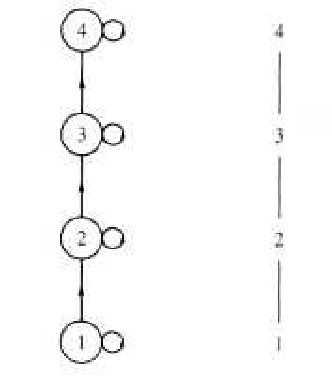
\includegraphics[width=0.5\linewidth]{images/fig-sol-6-2-1.png}
\caption*{\textbf{Figure 6.2.7:} }
\end{figure}
\end{divisionsolution}%
\begin{divisionsolution}{6.2.2.2}{}{exercise-233}%
\hypertarget{p-1993}{}%
Let \(B = \{1,2, 3, 4, 6, 8, 12, 24\}\), and let \(s\) be the relation ``divides'' on \(B\). Draw a digraph for \(s\).%
\end{divisionsolution}%
\begin{divisionsolution}{6.2.2.3}{}{exercise-234}%
\hypertarget{p-1994}{}%
Let \(A=\{1,2,3,4,5\}\). Define \(t\) on \(A\) by \(a t b\) if and only if \(b - a\) is even. Draw a digraph for \(t\).%
\par\smallskip%
\noindent\textbf{Answer}.\quad%
\hypertarget{p-1995}{}%
See Figure~6.2.8%
\begin{figure}
\centering
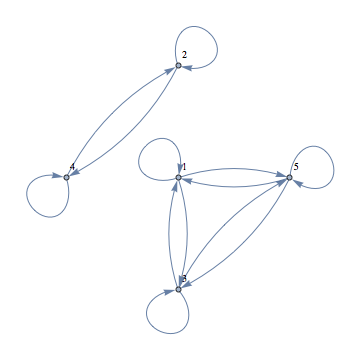
\includegraphics[width=0.6\linewidth]{images/fig-13-1-1.png}
\caption*{\textbf{Figure 6.2.8:} Digraph of the relation \(t\)}
\end{figure}
\end{divisionsolution}%
\begin{divisionsolution}{6.2.2.4}{}{exercise-235}%
\hypertarget{p-1996}{}%
\leavevmode%
\begin{enumerate}[label=(\alph*)]
\item\hypertarget{li-1059}{}Let \(A\) be the set of strings of 0's and 1's of length 3 or less. Define the relation of \(d\) on \(A\) by \(x d y\) if \(x\) is contained within \(y\). For example, \(01 d 101\). Draw a digraph for this relation.%
\item\hypertarget{li-1060}{}Do the same for the relation \(p\) defined by \(x p y\) if \(x\) is a prefix of \(y\). For example, \(10 p 101\), but \(01 p 101\) is false.%
\end{enumerate}
%
\end{divisionsolution}%
\begin{divisionsolution}{6.2.2.5}{}{exercise-236}%
\hypertarget{p-1997}{}%
Recall the relation in Exercise 5 of Section 6.1, \(\rho\) defined on the power set, \(\mathcal{P}(S)\), of a set \(S\). The definition was \((A,B) \in \rho\) iff \(A\cap  B = \emptyset\). Draw the digraph for \(\rho\) where \(S = \{a, b\}\).%
\end{divisionsolution}%
\begin{divisionsolution}{6.2.2.6}{}{exercise-237}%
\hypertarget{p-1998}{}%
Let \(C= \{1,2, 3, 4, 6, 8, 12, 24\}\) and define \(t\) on \(C\) by \(a t b\) if and only if \(a\) and \(b\) share a common divisor greater than 1.  Draw a digraph for \(t\).%
\end{divisionsolution}%
\section*{6.3 Properties of Relations}
\addcontentsline{toc}{section}{6.3 Properties of Relations}
\sectionmark{6.3 Properties of Relations}
\subsection*{6.3.4 Exercises for Section 6.3}
\addcontentsline{toc}{subsection}{6.3.4 Exercises for Section 6.3}
\begin{divisionsolution}{6.3.4.1}{}{exercise-238}%
\hypertarget{p-2049}{}%
\leavevmode%
\begin{enumerate}[label=(\alph*)]
\item\hypertarget{li-1078}{}\hypertarget{p-2050}{}%
Let \(B = \{a, b\}\) and \(U = \mathcal{P}(B)\). Draw a Hasse diagram for \(\subseteq \) on \(U\).%
\item\hypertarget{li-1079}{}\hypertarget{p-2051}{}%
Let \(A = \{1,2, 3, 6\}\). Show that divides, \(\mid \), is a partial ordering on \(A\).%
\item\hypertarget{li-1080}{}\hypertarget{p-2052}{}%
Draw a Hasse diagram for divides on \(A\).%
\item\hypertarget{li-1081}{}\hypertarget{p-2053}{}%
Compare the graphs of parts a and c.%
\end{enumerate}
%
\par\smallskip%
\noindent\textbf{Answer}.\quad%
\leavevmode%
\begin{figure}
\centering
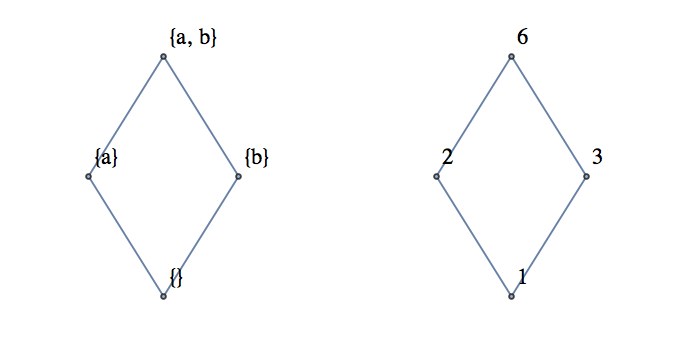
\includegraphics[width=1\linewidth]{images/fig-sol-6-3-1.png}
\caption*{\textbf{Figure 6.3.16:} }
\end{figure}
\hypertarget{p-2054}{}%
\leavevmode%
\begin{enumerate}[label=(\alph*)]
\item\hypertarget{li-1082}{}\hypertarget{p-2055}{}%
See Figure~6.3.16.%
\item\hypertarget{li-1083}{}\hypertarget{p-2056}{}%
The graphs are the same if we disregard the names of the vertices.%
\end{enumerate}
%
\end{divisionsolution}%
\begin{divisionsolution}{6.3.4.2}{}{exercise-239}%
\hypertarget{p-2057}{}%
Repeat Exercise 1 with \(B = \{a, b, c\}\) and \(A = \{1, 2, 3, 5, 6, 10, 15, 30\}\).%
\par\smallskip%
\noindent\textbf{Hint}.\quad%
\hypertarget{p-2058}{}%
Here is a Hasse diagram for the part (a).%
\begin{figure}
\centering
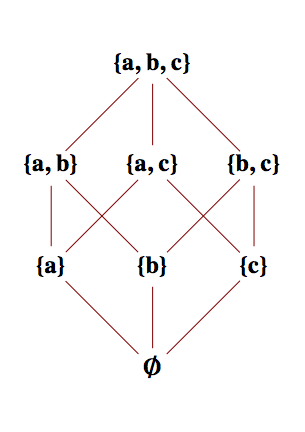
\includegraphics[width=1\linewidth]{images/fig-subsets-3-hasse.png}
\caption*{\textbf{Figure 6.3.17:} }
\end{figure}
\end{divisionsolution}%
\begin{divisionsolution}{6.3.4.3}{}{exercise-240}%
\hypertarget{p-2059}{}%
Consider the relations defined by the digraphs in Figure~6.3.18.\leavevmode%
\begin{enumerate}[label=(\alph*)]
\item\hypertarget{li-1084}{}\hypertarget{p-2060}{}%
Determine whether the given relations are reflexive, symmetric, antisymmetric, or transitive. Try to develop procedures for determining the validity of these properties from the graphs,%
\item\hypertarget{li-1085}{}\hypertarget{p-2061}{}%
Which of the graphs are of equivalence relations or of partial orderings?%
\end{enumerate}
%
\begin{figure}
\centering
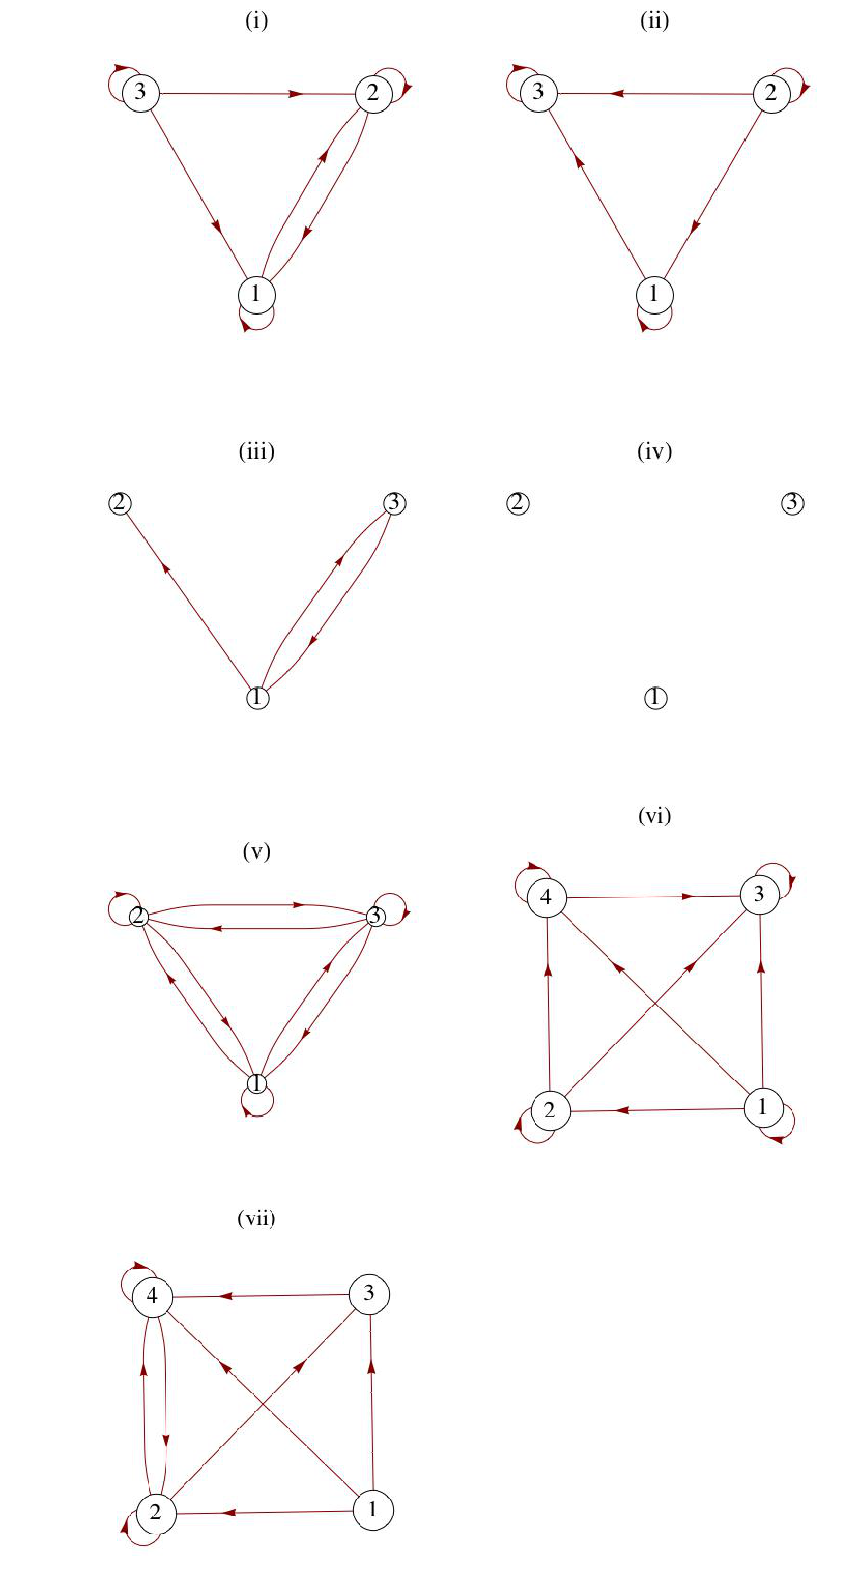
\includegraphics[width=1\linewidth]{images/exercises-6-digraphs.png}
\caption*{\textbf{Figure 6.3.18:} Some digraphs of relations}
\end{figure}
\par\smallskip%
\noindent\textbf{Answer}.\quad%
\leavevmode%
\begin{table}
\centering
\begin{tabular}{lllll}
Part&reflexive?&symmetric?&antisymmetric?&transitive?\tabularnewline[0pt]
i&yes&no&no&yes\tabularnewline[0pt]
ii&yes&no&yes&yes\tabularnewline[0pt]
iii&no&yes&no&yes\tabularnewline[0pt]
iv&no&yes&yes&yes\tabularnewline[0pt]
v&yes&yes&no&yes\tabularnewline[0pt]
vi&yes&no&yes&yes\tabularnewline[0pt]
vii&no&no&no&no
\end{tabular}
\caption*{\textbf{Table 6.3.19:} Properties of relations in number 3}
\end{table}
\hypertarget{p-2062}{}%
\leavevmode%
\begin{enumerate}[label=(\roman*)]
\item\hypertarget{li-1086}{}\hypertarget{p-2063}{}%
See Table~6.3.19%
\item\hypertarget{li-1087}{}\hypertarget{p-2064}{}%
Graphs ii and vi show partial ordering relations. Graph v is of an equivalence relation.%
\end{enumerate}
%
\end{divisionsolution}%
\begin{divisionsolution}{6.3.4.4}{}{exercise-241}%
\hypertarget{p-2065}{}%
Determine which of the following are equivalence relations and\slash{}or partial ordering relations for the given sets:%
\par
\hypertarget{p-2066}{}%
\leavevmode%
\begin{enumerate}[label=(\alph*)]
\item\hypertarget{li-1088}{}\hypertarget{p-2067}{}%
\(A = \{\textrm{ lines in the plane}\}\), and \(r\) defined by  \(x r y\) if and only if \(x\) is parallel to \(y\).  Assume every line is parallel to itself.%
\item\hypertarget{li-1089}{}\hypertarget{p-2068}{}%
\(A = \mathbb{R}\) and \(r\) defined by  \(x r y\) if and only if \(\lvert x -y \rvert \leq  7\).%
\end{enumerate}
%
\end{divisionsolution}%
\begin{divisionsolution}{6.3.4.5}{}{exercise-242}%
\hypertarget{p-2069}{}%
Consider the  relation on \(\{1, 2, 3, 4, 5, 6\}\) defined by  \(r = \{(i,j):\enspace \lvert i - j\rvert  = 2\}\).%
\par
\hypertarget{p-2070}{}%
\leavevmode%
\begin{enumerate}[label=(\alph*)]
\item\hypertarget{li-1090}{}\hypertarget{p-2071}{}%
Is \(r\) reflexive?%
\item\hypertarget{li-1091}{}\hypertarget{p-2072}{}%
Is \(r\) symmetric?%
\item\hypertarget{li-1092}{}\hypertarget{p-2073}{}%
Is \(r\) transitive?%
\item\hypertarget{li-1093}{}\hypertarget{p-2074}{}%
Draw a graph of \(r\).%
\end{enumerate}
%
\par\smallskip%
\noindent\textbf{Answer}.\quad%
\hypertarget{p-2075}{}%
\leavevmode%
\begin{enumerate}[label=(\alph*)]
\item\hypertarget{li-1094}{}\hypertarget{p-2076}{}%
No, since \(\mid 1-1\mid =0\neq 2\), for example%
\item\hypertarget{li-1095}{}\hypertarget{p-2077}{}%
Yes, because \(\mid i-j\mid =\)\(\mid j-i\mid \).%
\item\hypertarget{li-1096}{}\hypertarget{p-2078}{}%
No, since \(\mid 2-4\mid =2\) and \(\mid 4-6\mid =2\), but \(\mid 2-6\mid =4\neq 2\), for example.%
\item\hypertarget{li-1097}{}\hypertarget{p-2079}{}%
See Figure~6.3.20%
\end{enumerate}
%
\begin{figure}
\centering

\includegraphics[width=1\linewidth]{images/fig-sol-6-3-5.png}
\caption*{\textbf{Figure 6.3.20:} }
\end{figure}
\end{divisionsolution}%
\begin{divisionsolution}{6.3.4.6}{}{exercise-243}%
\hypertarget{p-2080}{}%
For the set of cities on a map, consider the relation \(x r y\) if and only if city \(x\) is connected by a road to city \(y\). A city is considered to be connected to itself, and two cities are connected even though there are cities on the road between them. Is this an equivalence relation or a partial ordering? Explain.%
\end{divisionsolution}%
\begin{divisionsolution}{6.3.4.7}{Equivalence Classes.}{equivalence-classes}%
\hypertarget{p-2081}{}%
Let \(A = \{0, 1, 2, 3\}\) and let%
\begin{equation*}
r = \{(0, 0), (1, 1), (2, 2), (3, 3), (1, 2),(2, 1), (3, 2), (2, 3), (3, 1), (1, 3)\}
\end{equation*}
\leavevmode%
\begin{enumerate}[label=(\alph*)]
\item\hypertarget{li-1098}{}\hypertarget{p-2082}{}%
Verify that \(r\) is an equivalence relation on \(A\).%
\item\hypertarget{li-1099}{}\hypertarget{p-2083}{}%
Let \(a \in A\) and define \(c(a) = \{b \in A \mid a rb\}\). \label{notation-37} \(c(a)\) is called the \terminology{equivalence class of \(a\) under \(r\)}\index{Equivalence Class}. Find \(c(a)\) for each element \(a \in A\).%
\item\hypertarget{li-1100}{}\hypertarget{p-2084}{}%
Show that \(\{c(a) \mid  a \in A\}\) forms a partition of \(A\) for this set \(A\).%
\item\hypertarget{li-1101}{}\hypertarget{p-2085}{}%
Let \(r\) be an equivalence relation on an arbitrary set \(A\). Prove that the set of all equivalence classes under \(r\) constitutes a partition of \(A\).%
\end{enumerate}
%
\par\smallskip%
\noindent\textbf{Answer}.\quad%
\hypertarget{p-2086}{}%
\leavevmode%
\begin{enumerate}[label=(\alph*)]
\item\hypertarget{li-1102}{}%
\item\hypertarget{li-1103}{}\hypertarget{p-2087}{}%
\(c(0)=\{0\}, c(1)=\{1,2,3\}=c(2)=c(3)\)%
\item\hypertarget{li-1104}{}\hypertarget{p-2088}{}%
\(c(0)\cup c(1)=A\) and \(c(0)\cap c(1)=\emptyset\)%
\item\hypertarget{li-1105}{}\hypertarget{p-2089}{}%
Let \(A\) be any set and let \(r\) be an equivalence relation on \(A\). Let \(a\) be any element of \(A\). \(a\in c(a)\) since \(r\) is reflexive, so each element of \(A\) is in some equivalence class. Therefore, the union of all equivalence classes equals \(A\). Next we show that any two equivalence classes are either identical or disjoint and we are done. Let \(c(a)\) and \(c(b)\) be two equivalence classes, and assume that \(c(a)\cap c(b)\neq \emptyset\). We want to show that \(c(a)=c(b)\). To show that \(c(a)\subseteq c(b)\), let \(x\in c(a)\). \(x\in c(a) \Rightarrow a r x \). Also, there exists an element, \(y\), of \(A\) that is in the intersection of \(c(a)\) and \(c(b)\) by our assumption. Therefore,%
\begin{equation*}
\begin{split}
a r y \land b r y &\Rightarrow  a r y \land y r b \quad r\textrm{  is symmetric}\\
&\Rightarrow  a r b  \quad \textrm{ transitivity of }r \\
\end{split}
\end{equation*}
%
\par
\hypertarget{p-2090}{}%
Next,%
\begin{equation*}
\begin{split}
a r x \land a r b &\Rightarrow x r a \land a r b\\
&\Rightarrow  x r b\\
&\Rightarrow  b r x\\
& \Rightarrow  x \in c(b)\\
\end{split}
\end{equation*}
%
\par
\hypertarget{p-2091}{}%
Similarly, \(c(b)\subseteq c(a)\).  \(\square\)%
\end{enumerate}
%
\end{divisionsolution}%
\begin{divisionsolution}{6.3.4.8}{}{exercise-245}%
\hypertarget{p-2092}{}%
Define \(r\) on the power set of \(\{1, 2, 3\}\) by \(A r B \Leftrightarrow  \lvert A \rvert = \lvert B \rvert \). Prove that \(r\) is an equivalence relation. What are the equivalence classes under \(r\)?%
\end{divisionsolution}%
\begin{divisionsolution}{6.3.4.9}{}{exercise-246}%
\hypertarget{p-2093}{}%
Consider the following relations on \(\mathbb{Z}_8= \{0, 1, . . . , 7\}\). Which are equivalence relations? For the equivalence relations, list the equivalence classes.%
\par
\hypertarget{p-2094}{}%
\leavevmode%
\begin{enumerate}[label=(\alph*)]
\item\hypertarget{li-1106}{}\hypertarget{p-2095}{}%
\(a r b\) iff the English spellings of \(a\) and \(b\) begin with the same letter.%
\item\hypertarget{li-1107}{}\hypertarget{p-2096}{}%
\(a s b\) iff \(a - b\) is a positive integer.%
\item\hypertarget{li-1108}{}\hypertarget{p-2097}{}%
\(a t b\) iff \(a-b\) is an even integer.%
\end{enumerate}
%
\par\smallskip%
\noindent\textbf{Answer}.\quad%
\hypertarget{p-2098}{}%
\leavevmode%
\begin{enumerate}[label=(\alph*)]
\item\hypertarget{li-1109}{}Equivalence Relation, \(c(0)=\{0\},c(1)=\{1\},c(2)=\{2,3\} =c(3),c(4)=\{4,5\}=c(5)\), and \(c(6)=\{6,7\}=c(7)\)%
\item\hypertarget{li-1110}{}\hypertarget{p-2099}{}%
Not an Equivalence Relation.%
\item\hypertarget{li-1111}{}\hypertarget{p-2100}{}%
Equivalence Relation, \(c(0)=\{0,2,4,6\}=c(2)=c(4)=c(6)\)  and \(c(1)=\{1,3,5,7\}=c(3)=c(5)=c(7)\)%
\end{enumerate}
%
\end{divisionsolution}%
\begin{divisionsolution}{6.3.4.10}{}{exercise-247}%
\hypertarget{p-2101}{}%
Building on Exercise~6.3.4.7:%
\par
\hypertarget{p-2102}{}%
\leavevmode%
\begin{enumerate}[label=(\alph*)]
\item\hypertarget{li-1112}{}\hypertarget{p-2103}{}%
Prove that congruence modulo \(m\) is transitive.%
\item\hypertarget{li-1113}{}\hypertarget{p-2104}{}%
What are the equivalence classes under congruence modulo 2?%
\item\hypertarget{li-1114}{}\hypertarget{p-2105}{}%
What are the equivalence classes under congruence modulo 10?%
\end{enumerate}
%
\end{divisionsolution}%
\begin{divisionsolution}{6.3.4.11}{}{exercise-248}%
\hypertarget{p-2106}{}%
In this exercise, we prove that implication is a partial ordering. Let \(A\) be any set of propositions.%
\par
\hypertarget{p-2107}{}%
\leavevmode%
\begin{enumerate}[label=(\alph*)]
\item\hypertarget{li-1115}{}\hypertarget{p-2108}{}%
Verify that \(q \to  q\) is a tautology, thereby showing that \(\Rightarrow\) is a reflexive relation on \(A\).%
\item\hypertarget{li-1116}{}Prove that \(\Rightarrow\) is antisymmetric on \(A\). Note: we do not use = when speaking of propositions, but rather equivalence, \(\Leftrightarrow\).%
\item\hypertarget{li-1117}{}\hypertarget{p-2109}{}%
Prove that \(\Rightarrow\) is transitive on \(A\).%
\item\hypertarget{li-1118}{}\hypertarget{p-2110}{}%
Given that \(q_i\) is the proposition \(n < i\) on \(\mathbb{N}\), draw the Hasse diagram for the relation \(\Rightarrow\) on \(\{q_1, q_2, q_3,\ldots \}\).%
\end{enumerate}
%
\par\smallskip%
\noindent\textbf{Answer}.\quad%
\hypertarget{p-2111}{}%
\leavevmode%
\begin{enumerate}[label=(\alph*)]
\item\hypertarget{li-1119}{}\hypertarget{p-2112}{}%
The proof follows from the biconditional equivalence in Table~3.4.4.%
\item\hypertarget{li-1120}{}\hypertarget{p-2113}{}%
Apply the chain rule.%
\item\hypertarget{li-1121}{}\hypertarget{p-2114}{}%
See Figure~6.3.21.%
\end{enumerate}
%
\begin{figure}
\centering
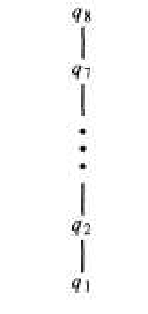
\includegraphics[width=0.4\linewidth]{images/fig-sol-6-3-11.png}
\caption*{\textbf{Figure 6.3.21:} }
\end{figure}
\end{divisionsolution}%
\begin{divisionsolution}{6.3.4.12}{}{exercise-6-3-12}%
\hypertarget{p-2115}{}%
Let \(S = \{1,2,3,4,5,6,7\}\) be a poset \((S, \leq )\) with the Hasse diagram shown below. Another relation \(r \subseteq  S\times S\) is defined as follows: \((x, y) \in  r\) if and only if there exists \(z \in S\) such that \(z < x\) and \(z < y\) in the poset \((S, \leq )\).%
\par
\hypertarget{p-2116}{}%
\leavevmode%
\begin{enumerate}[label=(\alph*)]
\item\hypertarget{li-1122}{}\hypertarget{p-2117}{}%
Prove that \(r\) is reflexive.%
\item\hypertarget{li-1123}{}\hypertarget{p-2118}{}%
Prove that \(r\) is symmetric.%
\item\hypertarget{li-1124}{}\hypertarget{p-2119}{}%
A compatible with respect to relation \(r\) is any subset \(Q\) of set \(S\) such that \(x \in  Q \textrm{ and } y \in Q \Rightarrow  (x, y) \in r\). A compatible \(g\) is a maximal compatible if \(Q\) is not a proper subset of another compatible. Give all maximal compatibles with respect to relation \(r\) defined above.%
\item\hypertarget{li-1125}{}\hypertarget{p-2120}{}%
Discuss a characterization of the set of maximal compatibles for relation \(r\) when \((S, \leq )\) is a general finite poset. What conditions, if any, on a general finite poset \((S, \leq )\) will make \(r\) an equivalence relation?%
\end{enumerate}
%
\begin{figure}
\centering
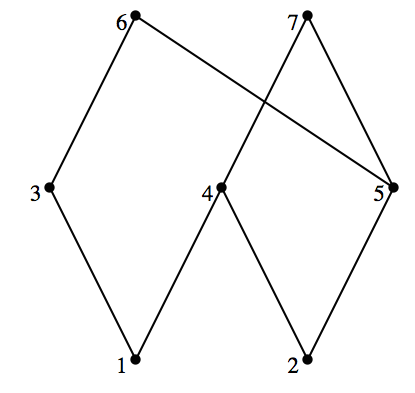
\includegraphics[width=1\linewidth]{images/exercise-6-12.png}
\caption*{\textbf{Figure 6.3.22:} Hasse diagram for \(r\) in exercise 12.}
\end{figure}
\end{divisionsolution}%
\section*{6.4 Matrices of Relations}
\addcontentsline{toc}{section}{6.4 Matrices of Relations}
\sectionmark{6.4 Matrices of Relations}
\subsection*{6.4.3 Exercises for Section 6.4}
\addcontentsline{toc}{subsection}{6.4.3 Exercises for Section 6.4}
\begin{divisionsolution}{6.4.3.1}{}{exercise-250}%
\hypertarget{p-2138}{}%
Let \(A_1 = \{1,2, 3, 4\}\), \(A_2 = \{4, 5, 6\}\), and \(A_3 = \{6, 7, 8\}\). Let \(r_1\) be the relation from \(A_1\) into \(A_2\) defined by \(r_1 = \{(x, y)  \mid  y - x = 2\}\), and let \(r_2\) be the relation from \(A_2\) into \(A_3\) defined by \(r_2 = \{(x, y) \mid  y - x = 1\}\).%
\par
\hypertarget{p-2139}{}%
\leavevmode%
\begin{enumerate}[label=(\alph*)]
\item\hypertarget{li-1130}{}\hypertarget{p-2140}{}%
Determine the adjacency matrices of \(r_1\) and \(r_2\).%
\item\hypertarget{li-1131}{}\hypertarget{p-2141}{}%
Use the definition of composition to find \(r_1r_2\).%
\item\hypertarget{li-1132}{}\hypertarget{p-2142}{}%
Verify the result in part b by finding the product of the adjacency matrices of \(r_1\) and \(r_2\).%
\end{enumerate}
%
\par\smallskip%
\noindent\textbf{Answer}.\quad%
\hypertarget{p-2143}{}%
\leavevmode%
\begin{enumerate}[label=(\alph*)]
\item\hypertarget{li-1133}{}\hypertarget{p-2144}{}%
\(\begin{array}{cc}
& 
\begin{array}{ccc}
4 & 5 & 6 \\
\end{array}
\\
\begin{array}{c}
1 \\
2 \\
3 \\
4 \\
\end{array}
& \left(
\begin{array}{ccc}
0 & 0 & 0 \\
1 & 0 & 0 \\
0 & 1 & 0 \\
0 & 0 & 1 \\
\end{array}
\right) \\
\end{array}\)  and \(\begin{array}{cc}
& 
\begin{array}{ccc}
6 & 7 & 8 \\
\end{array}
\\
\begin{array}{c}
4 \\
5 \\
6 \\
\end{array}
& \left(
\begin{array}{ccc}
0 & 0 & 0 \\
1 & 0 & 0 \\
0 & 1 & 0 \\
\end{array}
\right) \\
\end{array}\)%
\item\hypertarget{li-1134}{}\hypertarget{p-2145}{}%
\(r_1r_2 =\{(3,6),(4,7)\}\)%
\item\hypertarget{li-1135}{}\hypertarget{p-2146}{}%
\(\begin{array}{cc}
& 
\begin{array}{ccc}
6 & 7 & 8 \\
\end{array}
\\
\begin{array}{c}
1 \\
2 \\
3 \\
4 \\
\end{array}
& \left(
\begin{array}{ccc}
0 & 0 & 0 \\
0 & 0 & 0 \\
1 & 0 & 0 \\
0 & 1 & 0 \\
\end{array}
\right) \\
\end{array}\)%
\end{enumerate}
%
\end{divisionsolution}%
\begin{divisionsolution}{6.4.3.2}{}{exercise-251}%
\hypertarget{p-2147}{}%
\leavevmode%
\begin{enumerate}[label=(\alph*)]
\item\hypertarget{li-1136}{}\hypertarget{p-2148}{}%
Determine the adjacency matrix of each relation given via the digraphs in Exercise 3 of Section 6.3.%
\item\hypertarget{li-1137}{}\hypertarget{p-2149}{}%
Using the matrices found in part (a) above, find \(r^2\) of each relation in Exercise 3 of Section 6.3.%
\item\hypertarget{li-1138}{}\hypertarget{p-2150}{}%
Find the digraph of \(r^2\) directly from the given digraph and compare your results with those of part (b).%
\end{enumerate}
%
\end{divisionsolution}%
\begin{divisionsolution}{6.4.3.3}{}{exercise-252}%
\hypertarget{p-2151}{}%
Suppose that the matrices in Example~6.4.5 are relations on \(\{1, 2, 3, 4\}\). What relations do \(R\) and \(S\) describe?%
\par\smallskip%
\noindent\textbf{Answer}.\quad%
\leavevmode%
\begin{table}
\centering
\begin{tabular}{l}
R : \(x r y\) if and only if \(\lvert x -y \rvert = 1\)\tabularnewline[0pt]
S : \(x s y\) if and only if \(x\) is less than \(y\).
\end{tabular}
\caption*{\textbf{Table 6.4.8:} }
\end{table}
\end{divisionsolution}%
\begin{divisionsolution}{6.4.3.4}{}{exercise-253}%
\hypertarget{p-2152}{}%
Let \(D\) be the set of weekdays, Monday through Friday, let \(W\) be a set of employees \(\{1, 2, 3\}\) of a tutoring center, and let \(V\) be a set of computer languages for which tutoring is offered,  \(\{A(PL), B(asic), C(++), J(ava), L(isp), P(ython)\}\). We define \(s\) (schedule) from \(D\) into \(W\) by \(d s w\) if \(w\) is scheduled to work on day \(d\). We also define \(r\) from \(W\) into \(V\) by \(w r l\) if \(w\) can tutor students in language \(l\). If \(s\) and \(r\) are defined by matrices%
\par
\hypertarget{p-2153}{}%
%
\begin{equation*}
S = 
\begin{array}{cc}
& 
\begin{array}{ccc}
1 & 2 & 3 \\
\end{array}
\\
\begin{array}{c}
M \\
T \\
W \\
R \\
F \\
\end{array}
& 
\left(
\begin{array}{ccc}
1 & 0 & 1 \\
0 & 1 & 1 \\
1 & 0 & 1 \\
0 & 1 & 0 \\
1 & 1 & 0 \\
\end{array}
\right) \\
\end{array}
\textrm{ and }R=
\begin{array}{cc}
& 
\begin{array}{cccccc}
A & B & C & J & L & P \\
\end{array}
\\
\begin{array}{c}
1 \\
2 \\
3 \\
\end{array}
& \left(
\begin{array}{cccccc}
0 & 1 & 1 & 0 & 0 & 1 \\
1 & 1 & 0 & 1 & 0 & 1 \\
0 & 1 & 0 & 0 & 1 & 1 \\
\end{array}
\right) \\
\end{array}
\end{equation*}
%
\par
\hypertarget{p-2154}{}%
\leavevmode%
\begin{enumerate}[label=(\alph*)]
\item\hypertarget{li-1139}{}\hypertarget{p-2155}{}%
compute \(S R\) using Boolean arithmetic and give an interpretation of the relation it defines, and%
\item\hypertarget{li-1140}{}\hypertarget{p-2156}{}%
compute \(S R\) using regular arithmetic and give an interpretation of what the result describes.%
\end{enumerate}
%
\end{divisionsolution}%
\begin{divisionsolution}{6.4.3.5}{}{exercise-254}%
\hypertarget{p-2157}{}%
How many different reflexive, symmetric relations are there on a set with three elements?%
\par\smallskip%
\noindent\textbf{Hint}.\quad%
\hypertarget{p-2158}{}%
Consider the possible matrices.%
\par\smallskip%
\noindent\textbf{Answer}.\quad%
\hypertarget{p-2159}{}%
The diagonal entries of the matrix for such a relation must be 1. When the three entries above the diagonal are determined, the entries below are also determined. Therefore, there are \(2^3\) fitting the description.%
\end{divisionsolution}%
\begin{divisionsolution}{6.4.3.6}{}{exercise-255}%
\hypertarget{p-2160}{}%
Let \(A = \{a, b, c, d\}\).  Let \(r\) be the relation on \(A\) with adjacency matrix \(\begin{array}{cc}
& 
\begin{array}{cccc}
a & b & c & d \\
\end{array}
\\
\begin{array}{c}
a \\
b \\
c \\
c \\
\end{array}
& \left(
\begin{array}{cccc}
1 & 0 & 0 & 0 \\
0 & 1 & 0 & 0 \\
1 & 1 & 1 & 0 \\
0 & 1 & 0 & 1 \\
\end{array}
\right) \\
\end{array}\)%
\par
\hypertarget{p-2161}{}%
\leavevmode%
\begin{enumerate}[label=(\alph*)]
\item\hypertarget{li-1141}{}\hypertarget{p-2162}{}%
Explain why \(r\) is a partial ordering on \(A\).%
\item\hypertarget{li-1142}{}\hypertarget{p-2163}{}%
Draw its Hasse diagram.%
\end{enumerate}
%
\end{divisionsolution}%
\begin{divisionsolution}{6.4.3.7}{}{exercise-256}%
\hypertarget{p-2164}{}%
Define relations \(p\) and \(q\) on \(\{1, 2, 3, 4\}\) by \(p = \{(a, b) \mid \lvert a-b\rvert=1\}\) and \(q=\{(a,b) \mid a-b \textrm{ is even}\}\).%
\par
\hypertarget{p-2165}{}%
\leavevmode%
\begin{enumerate}[label=(\alph*)]
\item\hypertarget{li-1143}{}\hypertarget{p-2166}{}%
Represent \(p\) and \(q\) as both graphs and matrices.%
\item\hypertarget{li-1144}{}\hypertarget{p-2167}{}%
Determine \(p q\), \(p^2\), and \(q^2\); and represent them clearly in any way.%
\end{enumerate}
%
\par\smallskip%
\noindent\textbf{Answer}.\quad%
\hypertarget{p-2168}{}%
\leavevmode%
\begin{enumerate}[label=(\alph*)]
\item\hypertarget{li-1145}{}\hypertarget{p-2169}{}%
\(\begin{array}{cc}
& 
\begin{array}{cccc}
1 & 2 & 3 & 4 \\
\end{array}
\\
\begin{array}{c}
1 \\
2 \\
3 \\
4 \\
\end{array}
& \left(
\begin{array}{cccc}
0 & 1 & 0 & 0 \\
1 & 0 & 1 & 0 \\
0 & 1 & 0 & 1 \\
0 & 0 & 1 & 0 \\
\end{array}
\right) \\
\end{array}\) and \(\begin{array}{cc}
& 
\begin{array}{cccc}
1 & 2 & 3 & 4 \\
\end{array}
\\
\begin{array}{c}
1 \\
2 \\
3 \\
4 \\
\end{array}
& \left(
\begin{array}{cccc}
1 & 0 & 1 & 0 \\
0 & 1 & 0 & 1 \\
1 & 0 & 1 & 0 \\
0 & 1 & 0 & 1 \\
\end{array}
\right) \\
\end{array}\)%
\item\hypertarget{li-1146}{}\hypertarget{p-2170}{}%
\(P Q=
\begin{array}{cc}
& 
\begin{array}{cccc}
1 & 2 & 3 & 4 \\
\end{array}
\\
\begin{array}{c}
1 \\
2 \\
3 \\
4 \\
\end{array}
& \left(
\begin{array}{cccc}
0 & 1 & 0 & 0 \\
1 & 0 & 1 & 0 \\
0 & 1 & 0 & 1 \\
0 & 0 & 1 & 0 \\
\end{array}
\right) \\
\end{array}\) \(P^2 =\text{  }
\begin{array}{cc}
& 
\begin{array}{cccc}
1 & 2 & 3 & 4 \\
\end{array}
\\
\begin{array}{c}
1 \\
2 \\
3 \\
4 \\
\end{array}
& \left(
\begin{array}{cccc}
0 & 1 & 0 & 0 \\
1 & 0 & 1 & 0 \\
0 & 1 & 0 & 1 \\
0 & 0 & 1 & 0 \\
\end{array}
\right) \\
\end{array}\)\(=Q^2\)%
\end{enumerate}
%
\end{divisionsolution}%
\begin{divisionsolution}{6.4.3.8}{}{exercise-257}%
\hypertarget{p-2171}{}%
\leavevmode%
\begin{enumerate}[label=(\alph*)]
\item\hypertarget{li-1147}{}\hypertarget{p-2172}{}%
Prove that if \(r\) is a transitive relation on a set \(A\), then \(r^2 \subseteq  r\).%
\item\hypertarget{li-1148}{}\hypertarget{p-2173}{}%
Find an example of a transitive relation for which \(r^2\neq r\).%
\end{enumerate}
%
\end{divisionsolution}%
\begin{divisionsolution}{6.4.3.9}{}{exercise-258}%
\hypertarget{p-2174}{}%
We define \(\leq\) on the set of all \(n\times n\) relation matrices by the rule that if \(R\) and \(S\) are any two \(n\times n\) relation matrices, \(R \leq  S\) if and only if \(R_{ij} \leq S_{ij}\) for all \(1 \leq  i, j \leq  n\).%
\par
\hypertarget{p-2175}{}%
\leavevmode%
\begin{enumerate}[label=(\alph*)]
\item\hypertarget{li-1149}{}\hypertarget{p-2176}{}%
Prove that \(\leq\) is a partial ordering on all \(n\times n\) relation matrices.%
\item\hypertarget{li-1150}{}\hypertarget{p-2177}{}%
Prove that \(R \leq  S  \Rightarrow   R^2\leq S^2\) , but the converse is not true.%
\item\hypertarget{li-1151}{}\hypertarget{p-2178}{}%
If \(R\) and \(S\) are matrices of equivalence relations and \(R \leq  S\), how are the equivalence classes defined by \(R\) related to the equivalence classes defined by \(S\)?%
\end{enumerate}
%
\par\smallskip%
\noindent\textbf{Answer}.\quad%
\hypertarget{p-2179}{}%
\leavevmode%
\begin{enumerate}[label=(\alph*)]
\item\hypertarget{li-1152}{}\hypertarget{p-2180}{}%
Reflexive: \(R_{ij}=R_{ij}\) for all \(i,j\), therefore \(R_{ij}\leq R_{ij}\)%
\par
\hypertarget{p-2181}{}%
Antisymmetric: Assume \(R_{ij}\leq S_{ij}\) and \(S_{ij}\leq R_{ij}\) for all \(1\leq i,j\leq n\). Therefore, \(R_{ij} = S_{ij}\) for all \(1\leq i,j\leq n\)  and so \(R=S\)%
\par
\hypertarget{p-2182}{}%
Transitive: Assume \(R, S,\) and \(T\) are matrices where \(R_{ij}\leq S_{ij}\) and \(S_{ij}\leq T_{ij}\), for all \(1\leq i,j\leq n\). Then \(R_{ij}\leq T_{ij}\) for all \(1\leq i,j\leq n\), and so \(R\leq T\).%
\item\hypertarget{li-1153}{}\hypertarget{p-2183}{}%
%
\begin{equation*}
\begin{split}
\left(R^2\right)_{ij}&=R_{i1}R_{1j}+R_{i2}R_{2j}+\cdots +R_{in}R_{nj}\\
&\leq S_{i1}S_{1j}+S_{i2}S_{2j}+\cdots +S_{in}S_{nj}\\
&=\left(S^2\right)_{ij} \Rightarrow R^2\leq S^2
\end{split}\text{.}
\end{equation*}
%
\par
\hypertarget{p-2184}{}%
To verify that the converse is not true we need only one example. For \(n=2\), let \(R_{12}=1\) and all other entries equal \(0\), and let \(S\) be the zero matrix. Since \(R^2\) and \(S^2\) are both the zero matrix, \(R^2\leq S^2\), but since \(R_{12}>S_{12}, R\leq S\) is false.%
\item\hypertarget{li-1154}{}The matrices are defined on the same set \(A=\left\{a_1,a_2,\ldots  ,a_n\right\}\). Let \(c\left(a_i\right), i=1,2,\ldots  ,n\) be the equivalence classes defined by \(R\) and let \(d\left(a_i\right)\) be those defined by \(S\). Claim: \(c\left(a_i\right)\subseteq d\left(a_i\right)\).%
\begin{equation*}
\begin{split}
a_j\in c\left(a_i\right)&\Rightarrow a_i r a_j\\
&\Rightarrow R_{ij}=1 \Rightarrow S_{ij}=1\\
&\Rightarrow a_i s a_j\\ 
& \Rightarrow a_j \in d\left(a_i\right)\\
\end{split}
\end{equation*}
%
\end{enumerate}
%
\end{divisionsolution}%
\section*{6.5 Closure Operations on Relations}
\addcontentsline{toc}{section}{6.5 Closure Operations on Relations}
\sectionmark{6.5 Closure Operations on Relations}
\subsection*{6.5.3 Exercises for Section 6.5}
\addcontentsline{toc}{subsection}{6.5.3 Exercises for Section 6.5}
\begin{divisionsolution}{6.5.3.1}{}{exercise-259}%
\hypertarget{p-2210}{}%
Let \(A =\{0, 1, 2, 3, 4\}\) and \(\mathcal{S}=\{(0, 1), (1, 3), (2, 3), (3, 4), (4, 1)\}\). Compute \(\mathcal{S}^+\) using the matrix representation of \(\mathcal{S}\). Verify your results by checking against the result obtained directly from the definition of transitive closure.%
\end{divisionsolution}%
\begin{divisionsolution}{6.5.3.2}{}{exercise-260}%
\hypertarget{p-2211}{}%
Let \(A=\{1,2,3,4,6,12\}\) and \(t=\{(a,b)\mid b/a \textrm{ is a prime number}\}\). Determine \(t^+\) by any means.  Represent your answer as a matrix.%
\end{divisionsolution}%
\begin{divisionsolution}{6.5.3.3}{}{exercise-261}%
\hypertarget{p-2212}{}%
\leavevmode%
\begin{enumerate}[label=(\alph*)]
\item\hypertarget{li-1157}{}\hypertarget{p-2213}{}%
Draw digraphs of the relations \(\mathcal{S}\), \(\mathcal{S}^2\), \(\mathcal{S}^3\) , and \(\mathcal{S}^+\)  where \(\mathcal{S}\) is defined in the first exercise above.%
\item\hypertarget{li-1158}{}Verify that in terms of the graph of \(\mathcal{S}\), \(a \mathcal{S}^+ b\) if and only if \(b\) is reachable from \(a\) along a path of any finite nonzero length.%
\end{enumerate}
%
\par\smallskip%
\noindent\textbf{Answer}.\quad%
\hypertarget{p-2214}{}%
\leavevmode%
\begin{enumerate}[label=(\alph*)]
\item\hypertarget{li-1159}{}\hypertarget{p-2215}{}%
See graphs below.%
\item\hypertarget{li-1160}{}\hypertarget{p-2216}{}%
For example, \(0 s^+ 4\) and using \(S\) one can go from 0 to 4 using a path of length 3.%
\end{enumerate}
%
\begin{sidebyside}{2}{0.01}{0.01}{0.02}%
\begin{sbspanel}{0.48}%
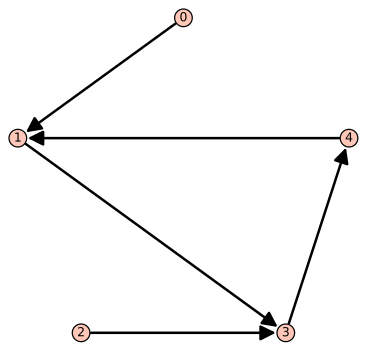
\includegraphics[width=1\linewidth]{images/S65-3s}
\end{sbspanel}%
\begin{sbspanel}{0.48}%
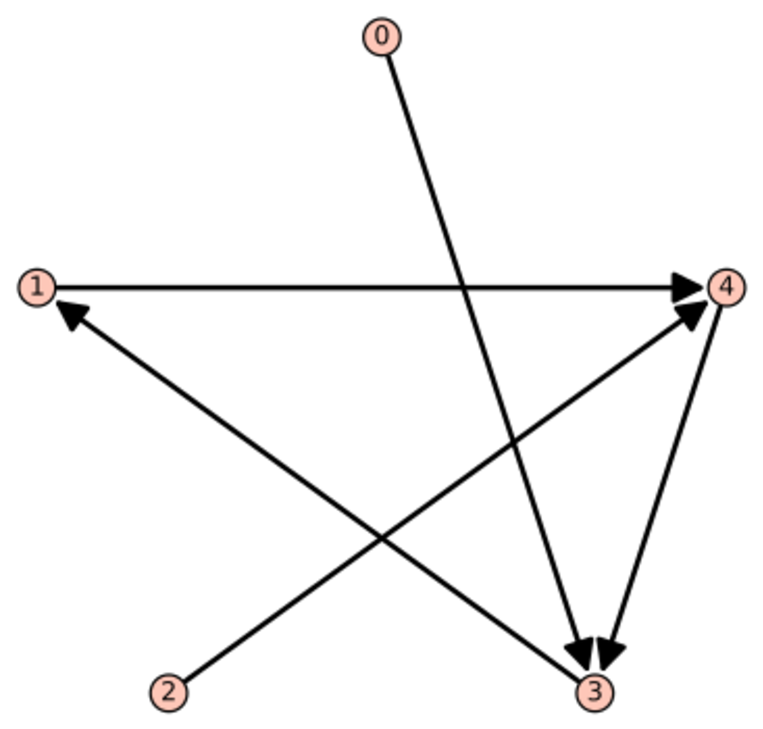
\includegraphics[width=1\linewidth]{images/S65-3s2}
\end{sbspanel}%
\nopagebreak%
\begin{sbscaption}{0.48}%
\captionof*{figure}{\textbf{Figure 6.5.10:} Digraph of \(\mathcal{S}\)}
\end{sbscaption}%
\begin{sbscaption}{0.48}%
\captionof*{figure}{\textbf{Figure 6.5.11:} Digraph of \(\mathcal{S}^2\)}
\end{sbscaption}%
\end{sidebyside}%
\begin{sidebyside}{2}{0.01}{0.01}{0.02}%
\begin{sbspanel}{0.48}%
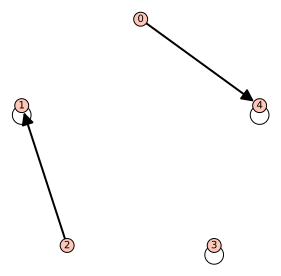
\includegraphics[width=1\linewidth]{images/S65-3s3}
\end{sbspanel}%
\begin{sbspanel}{0.48}%
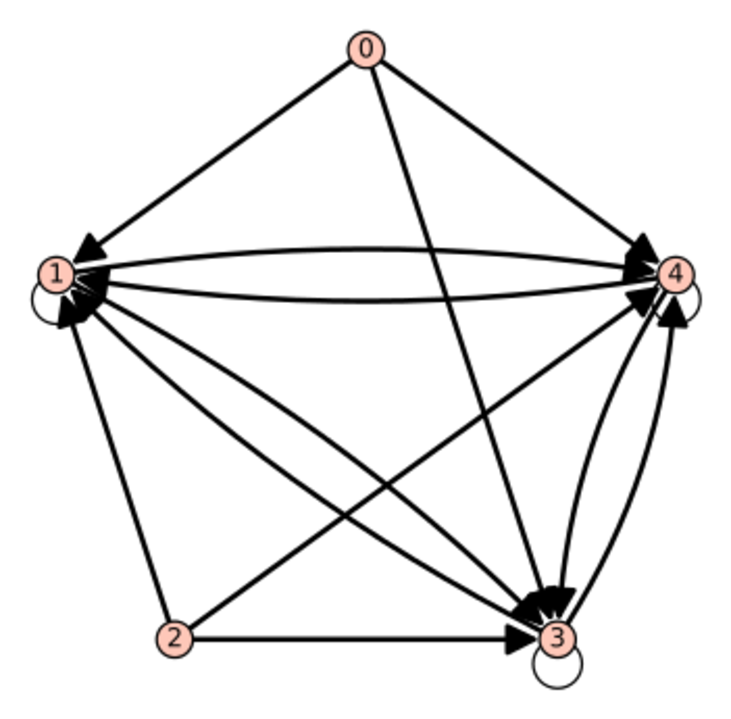
\includegraphics[width=1\linewidth]{images/S65-3stc}
\end{sbspanel}%
\nopagebreak%
\begin{sbscaption}{0.48}%
\captionof*{figure}{\textbf{Figure 6.5.12:} Digraph of \(\mathcal{S}^3\)}
\end{sbscaption}%
\begin{sbscaption}{0.48}%
\captionof*{figure}{\textbf{Figure 6.5.13:} Digraph of \(\mathcal{S}^+\)}
\end{sbscaption}%
\end{sidebyside}%
\end{divisionsolution}%
\begin{divisionsolution}{6.5.3.4}{}{exercise-262}%
\hypertarget{p-2217}{}%
Let \(r\) be the relation represented by the following digraph.%
\par
\hypertarget{p-2218}{}%
\leavevmode%
\begin{enumerate}[label=(\alph*)]
\item\hypertarget{li-1161}{}\hypertarget{p-2219}{}%
Find \(r^+\) using the definition based on order pairs.%
\item\hypertarget{li-1162}{}\hypertarget{p-2220}{}%
Determine the digraph of \(r^+\) directly from the digraph of \(r\).%
\item\hypertarget{li-1163}{}\hypertarget{p-2221}{}%
Verify your result in part (b) by computing the digraph from your result in part (a).%
\end{enumerate}
%
\begin{figure}
\centering
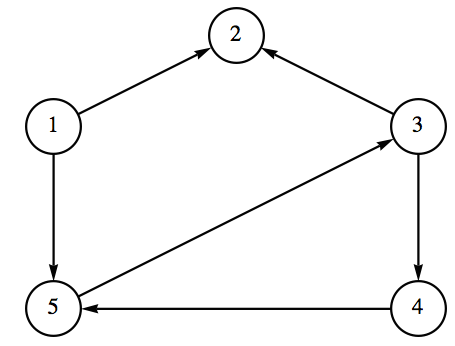
\includegraphics[width=0.9\linewidth]{images/fig-exercise-6-5-4.png}
\caption*{\textbf{Figure 6.5.14:} Digraph of \(r\) in exercise 4.}
\end{figure}
\end{divisionsolution}%
\begin{divisionsolution}{6.5.3.5}{}{exercise-263}%
\hypertarget{p-2222}{}%
\leavevmode%
\begin{enumerate}[label=(\alph*)]
\item\hypertarget{li-1164}{}\hypertarget{p-2223}{}%
Define reflexive closure and symmetric closure by imitating the definition of transitive closure.%
\item\hypertarget{li-1165}{}\hypertarget{p-2224}{}%
Use your definitions to compute the reflexive and symmetric closures of examples in the text.%
\item\hypertarget{li-1166}{}\hypertarget{p-2225}{}%
What are the transitive reflexive closures of these examples?%
\item\hypertarget{li-1167}{}\hypertarget{p-2226}{}%
Convince yourself that the reflexive closure of the relation \(<\) on the set of positive integers \(\mathbb{P}\) is \(\leq\).%
\end{enumerate}
%
\par\smallskip%
\noindent\textbf{Answer}.\quad%
\hypertarget{p-2227}{}%
Definition: Reflexive Closure.  Let \(r\) be a relation on \(A\). The reflexive closure of \(r\) is the smallest reflexive relation that contains \(r\).%
\par
\hypertarget{p-2228}{}%
Theorem: The reflexive closure of \(r\) is the union of \(r\) with \(\{(x, x) : x\in A\}\)%
\end{divisionsolution}%
\begin{divisionsolution}{6.5.3.6}{}{exercise-264}%
\hypertarget{p-2229}{}%
What common relations on \(\mathbb{Z}\) are the transitive closures of the following relations?%
\par
\hypertarget{p-2230}{}%
\leavevmode%
\begin{enumerate}[label=(\alph*)]
\item\hypertarget{li-1168}{}\hypertarget{p-2231}{}%
\(a S b\) if and only if \(a + 1 = b\).%
\item\hypertarget{li-1169}{}\hypertarget{p-2232}{}%
\(a R b\) if and only if \(| a - b | = 2\).%
\end{enumerate}
%
\end{divisionsolution}%
\begin{divisionsolution}{6.5.3.7}{}{exercise-265}%
\hypertarget{p-2233}{}%
\leavevmode%
\begin{enumerate}[label=(\alph*)]
\item\hypertarget{li-1170}{}\hypertarget{p-2234}{}%
Let \(A\) be any set and \(r\) a relation on \(A\), prove that \(\left(r^+\right)^+=r^+\).%
\item\hypertarget{li-1171}{}\hypertarget{p-2235}{}%
Is the transitive closure of a symmetric relation always both symmetric and reflexive? Explain.%
\end{enumerate}
%
\par\smallskip%
\noindent\textbf{Answer}.\quad%
\hypertarget{p-2236}{}%
\leavevmode%
\begin{enumerate}[label=(\alph*)]
\item\hypertarget{li-1172}{}\hypertarget{p-2237}{}%
By the definition of transitive closure, \(r^+\) is the smallest relation which contains \(r\); therefore, it is transitive. The transitive closure of \(r^+\), \(\left(r^+\right)^+\) , is the smallest transitive relation that contains \(r^+\). Since \(r^+\) is transitive, \(\left(r^+\right)^+=r^+\).%
\item\hypertarget{li-1173}{}\hypertarget{p-2238}{}%
The transitive closure of a symmetric relation is symmetric, but it may not be reflexive. If one element is not related to any elements, then the transitive closure will not relate that element to others.%
\end{enumerate}
%
\end{divisionsolution}%
\begin{divisionsolution}{6.5.3.8}{}{exercise-266}%
\hypertarget{p-2239}{}%
The definition of the Transitive Closure of \(r\) refers to the ``smallest transitive relation that contains \(r\) as a subset.''  Show that the intersection of all transitive relations on \(A\) containing \(r\) is a transitive relation containing \(r\) and is precisely \(r^+\).%
\end{divisionsolution}%
\chapter*{7 Functions}
\addcontentsline{toc}{chapter}{7 Functions}
\chaptermark{7 Functions}
\section*{7.1 Definition and Notation}
\addcontentsline{toc}{section}{7.1 Definition and Notation}
\sectionmark{7.1 Definition and Notation}
\subsection*{7.1.5 Exercises for Section 7.1}
\addcontentsline{toc}{subsection}{7.1.5 Exercises for Section 7.1}
\begin{divisionsolution}{7.1.5.1}{}{exercise-7-1-1}%
\hypertarget{p-2272}{}%
Let \(A = \{1, 2, 3, 4\}\) and \(B = \{a, b, c, d\}\). Determine which of the following are functions. Explain.%
\par
\hypertarget{p-2273}{}%
\leavevmode%
\begin{enumerate}[label=(\alph*)]
\item\hypertarget{li-1176}{}\hypertarget{p-2274}{}%
\(f \subseteq  A \times  B\), where \(f = \{(1, a), (2, b), (3, c), (4, d)\}\).%
\item\hypertarget{li-1177}{}\hypertarget{p-2275}{}%
\(g\subseteq A\times B\), where \(g = \{(1, a), (2, a), (3,b), (4,d)\}\).%
\item\hypertarget{li-1178}{}\hypertarget{p-2276}{}%
\(h \subseteq A \times  B\), where \(h = \{(1, a), (2, b), (3, c)\}\).%
\item\hypertarget{li-1179}{}\hypertarget{p-2277}{}%
\(k \subseteq A\times  B\), where \(k = \{(1, a), (2, b), (2, c), (3, a), (4, a)\}\).%
\item\hypertarget{li-1180}{}\hypertarget{p-2278}{}%
\(L\subseteq A\times A\), where \(L = \{(1, 1), (2, 1), (3, 1), (4, 1)\}\).%
\end{enumerate}
%
\par\smallskip%
\noindent\textbf{Answer}.\quad%
\hypertarget{p-2279}{}%
\leavevmode%
\begin{multicols}{3}
\begin{enumerate}[label=(\alph*)]
\item\hypertarget{li-1181}{}\hypertarget{p-2280}{}%
Yes%
\item\hypertarget{li-1182}{}\hypertarget{p-2281}{}%
Yes%
\item\hypertarget{li-1183}{}\hypertarget{p-2282}{}%
No%
\item\hypertarget{li-1184}{}\hypertarget{p-2283}{}%
No%
\item\hypertarget{li-1185}{}\hypertarget{p-2284}{}%
Yes%
\end{enumerate}
\end{multicols}
%
\end{divisionsolution}%
\begin{divisionsolution}{7.1.5.2}{}{exercise-characteristic-function}%
\hypertarget{p-2285}{}%
Let \(A\) be a set and let \(S\) be any subset of \(A\). Let \(\chi_S: A\to \{0,1\}\) be defined by%
\begin{equation*}
\chi_S(x)= \left\{
\begin{array}{cc}
1 & \textrm{if } x\in S \\
0 & \textrm{if } x\notin S \\
\end{array}
\right.
\end{equation*}
%
\par
\hypertarget{p-2286}{}%
The function \(\chi_S\) is called the \terminology{characteristic function}\index{Characteristic function} of \(S\).%
\par
\hypertarget{p-2287}{}%
\leavevmode%
\begin{enumerate}[label=(\alph*)]
\item\hypertarget{li-1186}{}\hypertarget{p-2288}{}%
If \(A = \{a, b, c\}\) and \(S = \{a, b\}\), list the elements of \(\chi_S\) .%
\item\hypertarget{li-1187}{}\hypertarget{p-2289}{}%
If \(A = \{a, b, c, d, e\}\) and \(S = \{a, c, e\}\), list the elements of \(\chi_S\).%
\item\hypertarget{li-1188}{}\hypertarget{p-2290}{}%
If \(A = \{a, b, c\}\), what are \(\chi_{\emptyset}\) and \(\chi_A\)?%
\end{enumerate}
%
\end{divisionsolution}%
\begin{divisionsolution}{7.1.5.3}{}{exercise-269}%
\hypertarget{p-2291}{}%
Find the ranges of each of the relations that are functions in Exercise 1.%
\par\smallskip%
\noindent\textbf{Answer}.\quad%
\hypertarget{p-2292}{}%
\leavevmode%
\begin{enumerate}[label=(\alph*)]
\item\hypertarget{li-1189}{}\hypertarget{p-2293}{}%
Range of \(f=f(A)=\{a,b,c,d\}=B\)%
\item\hypertarget{li-1190}{}\hypertarget{p-2294}{}%
Range of \(g=g(A)=\{a,b,d\}\)%
\item\hypertarget{li-1191}{}\hypertarget{p-2295}{}%
Range of \(L=L(A)=\{1\}\)%
\end{enumerate}
%
\end{divisionsolution}%
\begin{divisionsolution}{7.1.5.4}{}{exercise-270}%
\hypertarget{p-2296}{}%
Find the ranges of the following functions on \(\mathbb{Z}\):%
\par
\hypertarget{p-2297}{}%
\leavevmode%
\begin{enumerate}[label=(\alph*)]
\item\hypertarget{li-1192}{}\hypertarget{p-2298}{}%
\(g = \{(x, 4x +1)|x \in  \mathbb{Z}\}\).%
\item\hypertarget{li-1193}{}\hypertarget{p-2299}{}%
\(h(x) = \textrm{the least integer that is greater than or equal to } \sqrt{|x|}\).%
\item\hypertarget{li-1194}{}\hypertarget{p-2300}{}%
\(P(x) = x + 10\).%
\end{enumerate}
%
\end{divisionsolution}%
\begin{divisionsolution}{7.1.5.5}{}{exercise-271}%
\hypertarget{p-2301}{}%
Let \(f:\mathbb{P}\to \mathbb{P}\), where \(f(a)\) is the largest power of two that evenly divides \(a\); for example, \(f(12)=4,f(9)=1,\text{and}
f(8)=8\). Describe the equivalence classes of the kernel of \(f\).%
\end{divisionsolution}%
\begin{divisionsolution}{7.1.5.6}{}{exercise-272}%
\hypertarget{p-2302}{}%
Let \(U\) be a set with subsets \(A\) and \(B\).%
\par
\hypertarget{p-2303}{}%
\leavevmode%
\begin{enumerate}[label=(\alph*)]
\item\hypertarget{li-1195}{}\hypertarget{p-2304}{}%
Show that \(g:U\to \{0,1\}\) defined by \(g(a)=\min \left(C_A(a),C_B(a)\right)\) is the characteristic function of \(A\cap B\).%
\item\hypertarget{li-1196}{}\hypertarget{p-2305}{}%
What characteristic function is \(h:U\to \{0,1\}\) defined by \(h(a)=\max \left(C_A(a),C_B(a)\right)\)?%
\item\hypertarget{li-1197}{}\hypertarget{p-2306}{}%
How are the characteristic functions of \(A\) and \(A^c\) related?%
\end{enumerate}
%
\end{divisionsolution}%
\begin{divisionsolution}{7.1.5.7}{}{exercise-counting-functions}%
\hypertarget{p-2307}{}%
If \(A\) and \(B\) are finite sets, how many different functions are there from \(A\) into \(B\)?%
\par\smallskip%
\noindent\textbf{Answer}.\quad%
\hypertarget{p-2308}{}%
For each of the \(\lvert A \rvert \) elements of \(A\), there are \(\lvert B \rvert\) possible images, so there are \(\lvert B \rvert\cdot \lvert B \rvert\cdot \ldots \cdot \lvert B \rvert=\left\lvert B \rvert^{\lvert A \rvert}\right.\) functions from \(A\) into \(B\).%
\end{divisionsolution}%
\begin{divisionsolution}{7.1.5.8}{}{exercise-274}%
\hypertarget{p-2309}{}%
Let \(f\) be a function with domain \(A\) and codomain \(B\). Consider the relation \(K \subseteq  A \times  A\) defined on the domain of \(f\) by \((x, y) \in  K\) if and only if \(f(x) = f(y)\). The relation \(K\) is called \textbackslash{}textit\textbraceleft{} the kernel of f\textbraceright{}.%
\par
\hypertarget{p-2310}{}%
\leavevmode%
\begin{enumerate}[label=(\alph*)]
\item\hypertarget{li-1198}{}\hypertarget{p-2311}{}%
Prove that \(K\) is an equivalence relation.%
\item\hypertarget{li-1199}{}\hypertarget{p-2312}{}%
For the specific case of \(A = \mathbb{Z}\), where \(\mathbb{Z}\) is the set of integers, let \(f: \mathbb{Z} \rightarrow  \mathbb{Z}\) be defined by \(f(x) = x^2\). Describe the equivalence classes of the kernel for this specific function.%
\end{enumerate}
%
\end{divisionsolution}%
\section*{7.2 Properties of Functions}
\addcontentsline{toc}{section}{7.2 Properties of Functions}
\sectionmark{7.2 Properties of Functions}
\subsection*{7.2.3 Exercises for Section 7.2}
\addcontentsline{toc}{subsection}{7.2.3 Exercises for Section 7.2}
\begin{divisionsolution}{7.2.3.1}{}{exercise-275}%
\hypertarget{p-2344}{}%
Determine which of the functions in Exercise~7.1.5.1 of Section 7.1 are one- to-one and which are onto.%
\par\smallskip%
\noindent\textbf{Answer}.\quad%
\hypertarget{p-2345}{}%
The only one-to-one function and the only onto function is \(f\).%
\end{divisionsolution}%
\begin{divisionsolution}{7.2.3.2}{}{exercise-276}%
\hypertarget{p-2346}{}%
\leavevmode%
\begin{enumerate}[label=(\alph*)]
\item\hypertarget{li-1202}{}\hypertarget{p-2347}{}%
Determine all bijections from the \(\{1, 2, 3\}\) into \(\{a, b, c\}\).%
\item\hypertarget{li-1203}{}\hypertarget{p-2348}{}%
Determine all bijections from \(\{1, 2, 3\}\) into \(\{a, b, c, d\}\).%
\end{enumerate}
%
\end{divisionsolution}%
\begin{divisionsolution}{7.2.3.3}{}{exercise-277}%
\hypertarget{p-2349}{}%
Which of the following are one-to-one, onto, or both?%
\par
\hypertarget{p-2350}{}%
\leavevmode%
\begin{enumerate}[label=(\alph*)]
\item\hypertarget{li-1204}{}\hypertarget{p-2351}{}%
\(f_1:\mathbb{R} \rightarrow \mathbb{R}\) defined by \(f_1(x) = x^3 - x\).%
\item\hypertarget{li-1205}{}\hypertarget{p-2352}{}%
\(f_2 :\mathbb{Z} \rightarrow  \mathbb{Z}\) defined by \(f_2(x)= -x + 2\).%
\item\hypertarget{li-1206}{}\hypertarget{p-2353}{}%
\(f_3:\mathbb{N} \times \mathbb{N}\to \mathbb{N}\) defined by \(f_3(j, k) =2^j3^k\).%
\item\hypertarget{li-1207}{}\hypertarget{p-2354}{}%
\(f_4 :\mathbb{P} \rightarrow  \mathbb{P}\) defined by \(f_4(n)=\lceil n/2\rceil\), where \(\lceil x\rceil\) is the ceiling of \(x\), the smallest integer greater than or equal to \(x\).%
\item\hypertarget{li-1208}{}\hypertarget{p-2355}{}%
\(f_5 :\mathbb{N} \rightarrow  \mathbb{N}\) defined by \(f_5(n)=n^2+n\).%
\item\hypertarget{li-1209}{}\hypertarget{p-2356}{}%
\(f_6:\mathbb{N} \rightarrow  \mathbb{N} \times  \mathbb{N}\) defined by \(f_6(n)= (2n, 2n+1)\).%
\end{enumerate}
%
\par\smallskip%
\noindent\textbf{Answer}.\quad%
\hypertarget{p-2357}{}%
\leavevmode%
\begin{enumerate}[label=(\alph*)]
\item\hypertarget{li-1210}{}\hypertarget{p-2358}{}%
\(f_1\) is onto but not one-to-one: \(f_1(0)=f_1(1)\).%
\item\hypertarget{li-1211}{}\hypertarget{p-2359}{}%
\(f_2\) is  one-to-one and onto.%
\item\hypertarget{li-1212}{}\hypertarget{p-2360}{}%
\(f_3\) is  one-to-one but not onto.%
\item\hypertarget{li-1213}{}\hypertarget{p-2361}{}%
\(f_4\) is  onto but not one-to-one.%
\item\hypertarget{li-1214}{}\hypertarget{p-2362}{}%
\(f_5\) is  one-to-one but not onto.%
\item\hypertarget{li-1215}{}\hypertarget{p-2363}{}%
\(f_6\) is  one-to-one but not onto.%
\end{enumerate}
%
\end{divisionsolution}%
\begin{divisionsolution}{7.2.3.4}{}{exercise-278}%
\hypertarget{p-2364}{}%
Which of the following are injections, surjections, or bijections on \(\mathbb{R}\), the set of real numbers?%
\par
\hypertarget{p-2365}{}%
\leavevmode%
\begin{enumerate}[label=(\alph*)]
\item\hypertarget{li-1216}{}\hypertarget{p-2366}{}%
\(f(x) = -2x\).%
\item\hypertarget{li-1217}{}\hypertarget{p-2367}{}%
\(g(x) = x^2- 1\).%
\item\hypertarget{li-1218}{}\hypertarget{p-2368}{}%
\(h(x)=\left\{ \begin{array}{cc}
x & x < 0 \\
x^2 & x\geq 0 \\
\end{array} \right.\)%
\item\hypertarget{li-1219}{}\hypertarget{p-2369}{}%
\(q(x)=2^x\)%
\item\hypertarget{li-1220}{}\hypertarget{p-2370}{}%
\(r(x) =x^3\)%
\item\hypertarget{li-1221}{}\hypertarget{p-2371}{}%
\(s(x) = x^3-x\)%
\end{enumerate}
%
\end{divisionsolution}%
\begin{divisionsolution}{7.2.3.5}{}{exercise-279}%
\hypertarget{p-2372}{}%
Suppose that \(m\) pairs of socks are mixed up in your sock drawer. Use the Pigeonhole Principle to explain why, if you pick \(m + 1\) socks at random, at least two will make up a matching pair.%
\par\smallskip%
\noindent\textbf{Answer}.\quad%
\hypertarget{p-2373}{}%
Let \(X=\{\textrm{socks selected}\}\) and \(Y=\{\textrm{pairs of socks}\}\) and define \(f:X \to Y\) where \(f(x) =\)the pair of socks that \(x\) belongs to . By the Pigeonhole principle, there exist two socks that were selected from the same pair.%
\end{divisionsolution}%
\begin{divisionsolution}{7.2.3.6}{}{exercise-280}%
\hypertarget{p-2374}{}%
In your own words explain the statement ``The sets of integers and even integers have the same cardinality.''%
\end{divisionsolution}%
\begin{divisionsolution}{7.2.3.7}{}{exercise-281}%
\hypertarget{p-2375}{}%
Let \(A =\text{  }\{1, 2, 3, 4, 5\}\). Find functions, if they exist that have the properties specified below.%
\par
\hypertarget{p-2376}{}%
\leavevmode%
\begin{enumerate}[label=(\alph*)]
\item\hypertarget{li-1222}{}\hypertarget{p-2377}{}%
A function that is one-to-one and onto.%
\item\hypertarget{li-1223}{}\hypertarget{p-2378}{}%
A function that is neither one-to-one nor onto.%
\item\hypertarget{li-1224}{}\hypertarget{p-2379}{}%
A function that is one-to-one but not onto.%
\item\hypertarget{li-1225}{}\hypertarget{p-2380}{}%
A function that is onto but not one-to-one.%
\end{enumerate}
%
\par\smallskip%
\noindent\textbf{Answer}.\quad%
\hypertarget{p-2381}{}%
\leavevmode%
\begin{enumerate}[label=(\alph*)]
\item\hypertarget{li-1226}{}\hypertarget{p-2382}{}%
\(f(n)=n\), for example%
\item\hypertarget{li-1227}{}\hypertarget{p-2383}{}%
\(f(n)=1\), for example%
\item\hypertarget{li-1228}{}\hypertarget{p-2384}{}%
None exist.%
\item\hypertarget{li-1229}{}\hypertarget{p-2385}{}%
None exist.%
\end{enumerate}
%
\end{divisionsolution}%
\begin{divisionsolution}{7.2.3.8}{}{exercise-282}%
\hypertarget{p-2386}{}%
\leavevmode%
\begin{enumerate}[label=(\alph*)]
\item\hypertarget{li-1230}{}\hypertarget{p-2387}{}%
Define functions, if they exist, on the positive integers, \(\mathbb{P}\), with the same properties as in Exercise 7 (if possible).%
\item\hypertarget{li-1231}{}\hypertarget{p-2388}{}%
Let \(A\) and \(B\) be finite sets where \(|A|=|B|\). Is it possible to define a function \(f:A \rightarrow  B\) that is one-to-one but not onto? Is it possible to find a function  \(g:A \rightarrow  B\) that is onto but not one-to-one?%
\end{enumerate}
%
\end{divisionsolution}%
\begin{divisionsolution}{7.2.3.9}{}{exercise-283}%
\hypertarget{p-2389}{}%
\leavevmode%
\begin{enumerate}[label=(\alph*)]
\item\hypertarget{li-1232}{}\hypertarget{p-2390}{}%
Prove that the set of natural numbers is countable.%
\item\hypertarget{li-1233}{}\hypertarget{p-2391}{}%
Prove that the set of integers is countable.%
\item\hypertarget{li-1234}{}\hypertarget{p-2392}{}%
Prove that the set of rational numbers is countable.%
\end{enumerate}
%
\par\smallskip%
\noindent\textbf{Answer}.\quad%
\hypertarget{p-2393}{}%
\leavevmode%
\begin{enumerate}[label=(\alph*)]
\item\hypertarget{li-1235}{}\hypertarget{p-2394}{}%
Use \(s:\mathbb{N}\to \mathbb{P}\) defined by \(s(x)=x+1\).%
\item\hypertarget{li-1236}{}\hypertarget{p-2395}{}%
Use the function\(f:\mathbb{N}\to \mathbb{Z}\) defined by \(f(\text{x0}=x/2\) if \(x\) is even and \(f(x)=-(x+1)/2\) if \(x\) is odd.%
\item\hypertarget{li-1237}{}\hypertarget{p-2396}{}%
The proof is due to Georg Cantor (1845-1918), and involves listing the rationals through a definite procedure so that none are omitted and duplications are avoided. In the first row list all nonnegative rationals with denominator 1, in the second all nonnegative rationals with denominator 2, etc. In this listing, of course, there are duplications, for example, \(0/1=0/2=0\), \(1/1=3/3=1\), \(6/4=9/6=3/2\), etc. To obtain a list without duplications follow the arrows in Figure~7.2.13, listing only the circled numbers.%
\par
\hypertarget{p-2397}{}%
We obtain: \(0,1,1/2,2,3,1/3,1/4,2/3,3/2,4/1,\ldots\) Each nonnegative rational appears in this list exactly once. We now must insert in this list the negative rationals, and follow the same scheme to obtain:%
\begin{equation*}
0,1,-1,1/2,-1/2,2,-2,3,-3,1/3,-1/3, \ldots
\end{equation*}
which can be paired off with the elements of \(\mathbb{N}\).%
\end{enumerate}
%
\begin{figure}
\centering
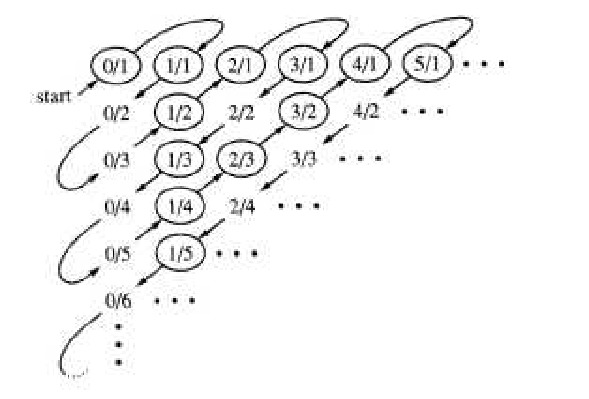
\includegraphics[width=1\linewidth]{images/fig-sol-7-2-9.png}
\caption*{\textbf{Figure 7.2.13:} Enumeration of the rational numbers.}
\end{figure}
\end{divisionsolution}%
\begin{divisionsolution}{7.2.3.10}{}{exercise-284}%
\hypertarget{p-2398}{}%
\leavevmode%
\begin{enumerate}[label=(\alph*)]
\item\hypertarget{li-1238}{}\hypertarget{p-2399}{}%
Prove that the set of finite strings of 0's and 1's is countable.%
\item\hypertarget{li-1239}{}\hypertarget{p-2400}{}%
Prove that the set of odd integers is countable.%
\item\hypertarget{li-1240}{}\hypertarget{p-2401}{}%
Prove that the set  \(\mathbb{N}\times  \mathbb{N}\) is countable.%
\end{enumerate}
%
\end{divisionsolution}%
\begin{divisionsolution}{7.2.3.11}{}{exercise-285}%
\hypertarget{p-2402}{}%
Use the Pigeonhole Principle to prove that an injection cannot exist between a finite set \(A\) and a finite set \(B\) if the cardinality of \(A\) is greater than the cardinality of \(B\).%
\par\smallskip%
\noindent\textbf{Answer}.\quad%
\hypertarget{p-2403}{}%
Let \(f\) be any function from \(A\) into \(B\). By the Pigeonhole principle with \(n=1\), there exists an element of \(B\) that is the image of at least two elements of \(A\). Therefore, \(f\) is not an injection.%
\end{divisionsolution}%
\begin{divisionsolution}{7.2.3.12}{}{exercise-286}%
\hypertarget{p-2404}{}%
The important properties of relations are not generally of interest for functions. Most functions are not reflexive, symmetric, antisymmetric, or transitive. Can you give examples of functions that do have these properties?%
\end{divisionsolution}%
\begin{divisionsolution}{7.2.3.13}{}{exercise-287}%
\hypertarget{p-2405}{}%
Prove that the set of all infinite sequences of 0's and 1's is not a countable set.%
\par\smallskip%
\noindent\textbf{Answer}.\quad%
\hypertarget{p-2406}{}%
The proof is indirect and follows a technique called the Cantor diagonal process. Assume to the contrary that the set is countable, then the elements can be listed: \(n_1,n_2,n_3,\ldots\) where each \(n_i\) is an infinite sequence of 0s and 1s. Consider the array:%
\begin{equation*}
\begin{array}{c}
n_1=n_{11}n_{12}n_{13}\cdots\\
n_2=n_{21}n_{22}n_{23}\cdots\\
n_3=n_{31}n_{32}n_{33}\cdots\\
\quad \vdots\\
\end{array}
\end{equation*}
%
\par
\hypertarget{p-2407}{}%
We assume that this array contains all infinite sequences of 0s and 1s. Consider the sequence \(s\) defined by \(s_i=\begin{cases}
0 & \textrm{ if } n_{\textrm{ii}}=1 \\
1 & \textrm{ if } n_{\textrm{ii}}=0
\end{cases}\)%
\par
\hypertarget{p-2408}{}%
Notice that \(s\) differs from each \(n_i\) in the \(i\)th position and so cannot be in the list. This is a contradiction, which completes our proof.%
\end{divisionsolution}%
\begin{divisionsolution}{7.2.3.13}{}{exercise-288}%
\hypertarget{p-2409}{}%
Prove that the set of all functions on the integers is an uncountable set.%
\end{divisionsolution}%
\begin{divisionsolution}{7.2.3.14}{}{exercise-289}%
\hypertarget{p-2410}{}%
Given five points on the unit square, \(\{(x,y) \mid 0 \leq x, y \leq 1 \}\), prove that there are two of the points a distance of no more than \(\frac{\sqrt{2}}{2}\) from one another.%
\end{divisionsolution}%
\section*{7.3 Function Composition}
\addcontentsline{toc}{section}{7.3 Function Composition}
\sectionmark{7.3 Function Composition}
\subsection*{7.3.4 Exercises for Section 7.3}
\addcontentsline{toc}{subsection}{7.3.4 Exercises for Section 7.3}
\begin{divisionsolution}{7.3.4.1}{}{exercise-290}%
\hypertarget{p-2454}{}%
Let \(A = \{1,2, 3, 4, 5\}\), \(B = \{a, b, c, d, e,f\}\), and \(C = \{+, -\}\). Define \(f: A \to  B\) by \(f(k)\) equal to the \(k^{th}\) letter in the alphabet, and define \(g : B \rightarrow  C\) by \(g(\alpha ) = +\) if \(\alpha\) is a vowel and \(g(\alpha ) = -\) if \(\alpha\) is a consonant.%
\par
\hypertarget{p-2455}{}%
\leavevmode%
\begin{enumerate}[label=(\alph*)]
\item\hypertarget{li-1243}{}\hypertarget{p-2456}{}%
Find \(g\circ  f\).%
\item\hypertarget{li-1244}{}\hypertarget{p-2457}{}%
Does it make sense to discuss \(f\circ g\)? If not, why not?%
\item\hypertarget{li-1245}{}\hypertarget{p-2458}{}%
Does \(f^{-1}\) exist? Why?%
\item\hypertarget{li-1246}{}\hypertarget{p-2459}{}%
Does \(g^{-1}\) exist? Why?%
\end{enumerate}
%
\par\smallskip%
\noindent\textbf{Answer}.\quad%
\hypertarget{p-2460}{}%
\leavevmode%
\begin{enumerate}[label=(\alph*)]
\item\hypertarget{li-1247}{}\(g\circ f:A\to C\) is defined by \((g\circ f)(k)=\begin{cases}
+ & \textrm{ if } k=1 \textrm{ or } k=5 \\
- & \textrm{ otherwise}
\end{cases}\)%
\item\hypertarget{li-1248}{}\hypertarget{p-2461}{}%
No, since the domain of \(f\) is not equal to the codomain of \(g\).%
\item\hypertarget{li-1249}{}\hypertarget{p-2462}{}%
No, since \(f\) is not surjective.%
\item\hypertarget{li-1250}{}\hypertarget{p-2463}{}%
No, since \(g\) is not injective.%
\end{enumerate}
%
\end{divisionsolution}%
\begin{divisionsolution}{7.3.4.2}{}{exercise-291}%
\hypertarget{p-2464}{}%
Let \(A = \{1, 2, 3\}\). Define\(f:A\rightarrow A\) by \(f(1) = 2\), \(f(2) = 1\), and \(f(3) = 3\). Find \(f^2\), \(f^3\), \(f^4\) and \(f^{-1}\).%
\end{divisionsolution}%
\begin{divisionsolution}{7.3.4.3}{}{exercise-292}%
\hypertarget{p-2465}{}%
Let \(A = \{1, 2, 3\}\).%
\par
\hypertarget{p-2466}{}%
\leavevmode%
\begin{enumerate}[label=(\alph*)]
\item\hypertarget{li-1251}{}\hypertarget{p-2467}{}%
List all permutations of \(A\).%
\item\hypertarget{li-1252}{}\hypertarget{p-2468}{}%
Find the inverse and square of each of the permutations of part a, where the square of a permutation, \(f\), is the composition \(f \circ f\).%
\item\hypertarget{li-1253}{}\hypertarget{p-2469}{}%
Show that the composition of any two permutations of \(A\) is a permutation of \(A\).%
\item\hypertarget{li-1254}{}\hypertarget{p-2470}{}%
Prove that if \(A\) is any set where \(\lvert A\rvert= n\), then the number of permutations of \(A\) is \(n!\).%
\end{enumerate}
%
\par\smallskip%
\noindent\textbf{Answer}.\quad%
\hypertarget{p-2471}{}%
\leavevmode%
\begin{enumerate}[label=(\alph*)]
\item\hypertarget{li-1255}{}\hypertarget{p-2472}{}%
The permutations of \(A\) are \(i,r_1,r_2,f_1,f_2,\) and \(f_3\), defined in Table~15.3.1.%
\item\hypertarget{li-1256}{}\hypertarget{p-2473}{}%
%
\begin{equation*}
\begin{array}{ccc}
g  & g^{-1} & g^2 \\
i & i & i \\
r_1 & r_2 & r_2  \\
r_2 & r_1 & r_1  \\
f_1 & f_1 & i \\
f_2 & f_2 & i  \\
f_3 & f_3 & i  \\
\end{array}
\end{equation*}
%
\item\hypertarget{li-1257}{}\hypertarget{p-2474}{}%
If \(f\) and \(g\) are permutations of \(A\), then they are both injections and their composition, \(f\circ g\), is a injection, by Theorem~7.3.6. By Theorem~7.3.7, \(f\circ g\) is also a surjection; therefore, \(f\circ g\) is a bijection on \(A\), a permutation.%
\item\hypertarget{li-1258}{}\hypertarget{p-2475}{}%
Proof by induction: Basis: \((n=1)\).  The number of permutations of \(A\) is one, the identity function, and 1! \(=1\).%
\par
\hypertarget{p-2476}{}%
Induction: Assume that the number of permutations on a set with \(n\) elements, \(n\geq 1\), is \(n\)!. Furthermore, assume that \(|A|=\)\(\text{  }n+1\) and that \(A\) contains an element called \(\sigma\). Let \(A'=A-\{\sigma\}\). We can reduce the definition of a permutation, \(f\), on \(A\) to two steps. First, we select any one of the \(n\)! permutations on \(A'\). (Note the use of the induction hypothesis.) Call it \(g\). This permutation almost completely defines a permutation on \(A\) that we will call  \(f\).  For all \(a\) in \(A'\), we start by defining \(f(a)\) to be \(g(a)\). We may be making some adjustments, but define it that way for now. Next, we select the image of \(\sigma\), which can be done \(n+1\) different ways, allowing for any value in \(A\). To keep our function bijective, we must adjust \(f\) as follows: If we select \(f(\sigma)=y \neq \sigma\), then we must find the element, \(z\), of \(A\) such that \(g(z)=y\), and redefine the image  of \(z\) to \(f(z)=\sigma\). If we had selected \(f(\sigma)=\sigma\), then there is  no adjustment needed. By the rule of products, the number of ways that we can define \(f\) is \(n!(n+1)=(n+1)!\) \(\square\)%
\end{enumerate}
%
\end{divisionsolution}%
\begin{divisionsolution}{7.3.4.4}{}{exercise-293}%
\hypertarget{p-2477}{}%
Define \(s\), \(u\), and \(d\), all functions on the integers, by \(s(n) = n^2\) , \(u(n) = n + 1\), and \(d(n) = n-1\). Determine:%
\par
\hypertarget{p-2478}{}%
\leavevmode%
\begin{enumerate}[label=(\alph*)]
\item\hypertarget{li-1259}{}\hypertarget{p-2479}{}%
\(u \circ  s \circ  d\)%
\item\hypertarget{li-1260}{}\hypertarget{p-2480}{}%
\(s \circ  u\circ  d\)%
\item\hypertarget{li-1261}{}\hypertarget{p-2481}{}%
\(d \circ  s \circ  u\)%
\end{enumerate}
%
\end{divisionsolution}%
\begin{divisionsolution}{7.3.4.5}{}{exercise-294}%
\hypertarget{p-2482}{}%
Based on the definition of the identity function, show that for all functions \(f:A\to A\), \(f\circ i=i\circ f = f\).%
\end{divisionsolution}%
\begin{divisionsolution}{7.3.4.6}{}{exercise-295}%
\hypertarget{p-2483}{}%
\terminology{Inverse images.} If \(f\) is any function from \(A\) into \(B\), we can describe the inverse image as a function from \(B\) into \(\mathcal{P}(A)\), which is also commonly denoted \(f^{-1}\). If \(b \in  B\), \(f^{-1}(b) = \{a \in A\mid f(a) = b\}\). If \(f\) does have an inverse, the inverse image of \(b\) is \(\left\{f^{-1}(b)\right\}\).%
\par
\hypertarget{p-2484}{}%
\leavevmode%
\begin{enumerate}[label=(\alph*)]
\item\hypertarget{li-1262}{}\hypertarget{p-2485}{}%
Let \(g : \mathbb{R} \to  \mathbb{R}\) be defined by \(g(x) = x^2\). What are \(g^{-1}(4)\), \(g^{-1}(0)\) and \(g^{-1}(-1)\)?%
\item\hypertarget{li-1263}{}\hypertarget{p-2486}{}%
If \(r: \mathbb{R}\to \mathbb{Z}\), where \(r(x) = \lceil x\rceil\),  what is \(r^{-1}(1)\)?%
\end{enumerate}
%
\end{divisionsolution}%
\begin{divisionsolution}{7.3.4.7}{}{exercise-296}%
\hypertarget{p-2487}{}%
Let \(f,\)  \(g\), and \(h\) all be functions from \(\mathbb{Z}\) into \(\mathbb{Z}\) defined by \(f(n) = n + 5\), \(g(n) = n - 2,\) and \(h(n)=n^2\). Define:%
\par
\hypertarget{p-2488}{}%
\leavevmode%
\begin{enumerate}[label=(\alph*)]
\item\hypertarget{li-1264}{}\hypertarget{p-2489}{}%
\(f\circ g\)%
\item\hypertarget{li-1265}{}\hypertarget{p-2490}{}%
\(f^3\)%
\item\hypertarget{li-1266}{}\hypertarget{p-2491}{}%
\(f\circ h\)%
\end{enumerate}
%
\par\smallskip%
\noindent\textbf{Answer}.\quad%
\hypertarget{p-2492}{}%
\leavevmode%
\begin{enumerate}[label=(\alph*)]
\item\hypertarget{li-1267}{}\hypertarget{p-2493}{}%
\(f\circ g(n)=n+3\)%
\item\hypertarget{li-1268}{}\hypertarget{p-2494}{}%
\(f^3(n)=n+15\)%
\item\hypertarget{li-1269}{}\hypertarget{p-2495}{}%
\(f\circ h(n)=n^2+5\)%
\end{enumerate}
%
\end{divisionsolution}%
\begin{divisionsolution}{7.3.4.8}{}{exercise-297}%
\hypertarget{p-2496}{}%
Define the following functions on the integers by \(f(k) = k + 1\), \(g(k) = 2k\), and \(h(k)=\lceil k/2\rceil\)%
\par
\hypertarget{p-2497}{}%
\leavevmode%
\begin{enumerate}[label=(\alph*)]
\item\hypertarget{li-1270}{}\hypertarget{p-2498}{}%
Which of these functions are one-to-one?%
\item\hypertarget{li-1271}{}\hypertarget{p-2499}{}%
Which of these functions are onto?%
\item\hypertarget{li-1272}{}\hypertarget{p-2500}{}%
Express in simplest terms the compositions \(f\circ g\), \(g \circ f\), \(g \circ  h\), \(h \circ  g\), and \(h^2\) ,%
\end{enumerate}
%
\end{divisionsolution}%
\begin{divisionsolution}{7.3.4.9}{}{exercise-298}%
\hypertarget{p-2501}{}%
Let \(A\) be a nonempty set. Prove that if \(f \) is a bijection on \(A\) and \(f \circ f=f\), then \(f\) is the identity function, \(i\)%
\par\smallskip%
\noindent\textbf{Hint}.\quad%
\hypertarget{p-2502}{}%
You have seen a similar proof in matrix algebra.%
\end{divisionsolution}%
\begin{divisionsolution}{7.3.4.10}{}{exercise-299}%
\hypertarget{p-2503}{}%
For the real matrix \(A=\left(
\begin{array}{cc}
a & b \\
c & d 
\end{array}
\right)\), \(\det(A)= a d-b c\).%
\par
\hypertarget{p-2504}{}%
Recall that a  \terminology{bijection} from a set to itself is also referred to as a \terminology{permutation} of the set. Let \(\pi\) be a permutation of \(\{a,b,c,d\}\) such that \(a\) becomes \(\pi (a)\), \(b\) becomes \(\pi (b)\), etc.%
\par
\hypertarget{p-2505}{}%
Let \(B=\left(
\begin{array}{cc}
\pi(a)& \pi(b)\\
\pi(c)& \pi(d)\\
\end{array}
\right)\). How many permutations of \(\pi\) leave the determinant of \(A\) invariant, that is, \(\det  A = \det  B\)?%
\end{divisionsolution}%
\begin{divisionsolution}{7.3.4.11}{}{exercise-300}%
\hypertarget{p-2506}{}%
State and prove a theorem on inverse functions analogous to the one that says that if a matrix has an inverse, that inverse is unique.%
\par\smallskip%
\noindent\textbf{Answer}.\quad%
\hypertarget{p-2507}{}%
If \(f:A\to B\) and \(f\) has an inverse, then that inverse is unique.%
\par
\hypertarget{p-2508}{}%
Proof:  Suppose that \(g\) and \(h\) are both inverses of \(f\), both having domain \(B\) and codomain \(A\).%
\begin{equation*}
\begin{split}g &= g\circ i_B \\
& =g\circ (f\circ h)\\
& =(g\circ f)\circ h\\
& =i_A\circ h\\
& =h\quad \Rightarrow g=h \quad \square
\end{split}
\end{equation*}
%
\end{divisionsolution}%
\begin{divisionsolution}{7.3.4.12}{}{exercise-301}%
\hypertarget{p-2509}{}%
Let \(f\) and \(g\) be functions whose inverses exist. Prove that \((f\circ g)^{-1}= g^{-1}\circ f^{-1}\).%
\par\smallskip%
\noindent\textbf{Hint}.\quad%
\hypertarget{p-2510}{}%
See Exercise 3 of Section 5.4.%
\end{divisionsolution}%
\begin{divisionsolution}{7.3.4.13}{}{exercise-302}%
\hypertarget{p-2511}{}%
Prove Theorem~7.3.6 and Theorem~7.3.7.%
\par\smallskip%
\noindent\textbf{Answer}.\quad%
\hypertarget{p-2512}{}%
Let \(x,x'\) be elements of \(A\) such that \(g\circ f(x)=g\circ f(x')\); that is, \(g(f(x))=g(f(x'))\). Since \(g\) is injective, \(f(x)=f(x')\) and since \(f\) is injective, \(x=x'\). \(\square\)%
\par
\hypertarget{p-2513}{}%
Let \(x\) be an element of \(C\). We must show that there exists an element of \(A\) whose image under \(g\circ f\) is \(x\). Since \(g\) is surjective, there exists an element of \(B\), \(y\), such that \(g(y)=x\). Also, since \(f\) is a surjection, there exists an element of \(A\), \(z\), such that \(f(z)=y\), \(g\circ f(z)=g(f(z))=g(y)=x\).\(\square\)%
\end{divisionsolution}%
\begin{divisionsolution}{7.3.4.14}{}{exercise-303}%
\hypertarget{p-2514}{}%
Prove the second half of Theorem~7.3.14.%
\end{divisionsolution}%
\begin{divisionsolution}{7.3.4.15}{}{exercise-304}%
\hypertarget{p-2515}{}%
Prove by induction that if \(n\geq  2\) and \(f_1\), \(f_2\) , \textbackslash{}ldots  , \(f_n\) are invertible functions on some nonempty set \(A\), then \textbraceleft{} \textbraceright{}\(\left( f_1\circ  f_2\circ  \cdots  \circ  f_n \right){}^{-1}= f_n^{-1}\circ \cdots \circ f_2^{-1}\circ f_1^{-1}\). The basis has been taken care of in Exercise 10.%
\par\smallskip%
\noindent\textbf{Answer}.\quad%
\hypertarget{p-2516}{}%
Basis: \((n=2)\): \(\left(f_1\circ f_2\right){}^{-1}=f_2{}^{-1}\circ f_1{}^{-2}\) by exercise 10.%
\par
\hypertarget{p-2517}{}%
Induction: Assume \(n\geq 2\) and%
\begin{equation*}
\left(f_1\circ f_2\circ \cdots \circ f_n\right){}^{-1}= f_n{}^{-1}\circ \cdots \circ f_2{}^{-1}\circ f_1{}^{-1}
\end{equation*}
and consider \(\left(f_1\circ f_2\circ \cdots \circ f_{n+1}\right)^{-1}\).%
\begin{equation*}
\begin{split}
\left(f_1\circ f_2\circ \cdots \circ f_{n+1}\right){}^{-1} &=\left(\left(f_1\circ f_2\circ \cdots \circ f_n\right)\circ f_{n+1}\right){}^{-1}\\
& =f_{n+1}{}^{-1}\circ \left(f_1\circ f_2\circ \cdots \circ f_n\right){}^{-1}\\
& \quad \quad \quad \textrm{ by the basis}\\
&=f_{n+1}{}^{-1}\circ \left(f_n{}^{-1}\circ \cdots \circ f_2{}^{-1}\circ f_1{}^{-1}\right)\\
& \quad \quad \quad \textrm{ by the induction hypothesis}\\
&=f_{n+1}{}^{-1}\circ \cdots \circ f_2{}^{-1}\circ f_1{}^{-1} \quad. \square
\end{split}
\end{equation*}
%
\end{divisionsolution}%
\begin{divisionsolution}{7.3.4.16}{}{exercise-305}%
\hypertarget{p-2518}{}%
\leavevmode%
\begin{enumerate}[label=(\alph*)]
\item\hypertarget{li-1273}{}Our definition of cardinality states that two sets, \(A\) and \(B\), have the same cardinality if there exists a bijection between the two sets. Why does it not matter whether the bijection is from \(A\) into \(B\) or \(B\) into \(A\)?%
\item\hypertarget{li-1274}{}\hypertarget{p-2519}{}%
Prove that ``has the same cardinality as'' is an equivalence relation on sets.%
\end{enumerate}
%
\end{divisionsolution}%
\begin{divisionsolution}{7.3.4.17}{}{exercise-306}%
\hypertarget{p-2520}{}%
Construct a table listing as many ``Laws of Function Composition'' as you can identify. Use previous lists of laws as a guide.%
\end{divisionsolution}%
\chapter*{8 Recursion and Recurrence Relations}
\addcontentsline{toc}{chapter}{8 Recursion and Recurrence Relations}
\chaptermark{8 Recursion and Recurrence Relations}
\section*{8.1 The Many Faces of Recursion}
\addcontentsline{toc}{section}{8.1 The Many Faces of Recursion}
\sectionmark{8.1 The Many Faces of Recursion}
\subsection*{8.1.8 Exercises for Section 8.1}
\addcontentsline{toc}{subsection}{8.1.8 Exercises for Section 8.1}
\begin{divisionsolution}{8.1.8.1}{}{exercise-307}%
\hypertarget{p-2565}{}%
By the recursive definition of binomial coefficients, \(\binom{7}{2}=\binom{6}{2} +\binom{6}{1}\). Continue expanding \(\binom{7}{2}\) to express it in terms of quantities defined by the basis. Check your result by applying the factorial definition of \(\binom{n}{k}\).%
\par\smallskip%
\noindent\textbf{Answer}.\quad%
\hypertarget{p-2566}{}%
%
\begin{equation*}
\begin{split}
\binom{7}{2} &=\binom{6}{2} +\binom{6}{1} \\
&=\binom{5}{2} +\binom{5}{1} +\binom{5}{1} +\binom{5}{0} \\
&=\binom{5}{2} +2 \binom{5}{1} +1\\
&=\binom{4}{2} +\binom{4}{1} +2(\binom{4}{1} +\binom{4}{0} )+1\\
&=\binom{4}{2} +3 \binom{4}{1} + 3\\
&=\binom{3}{2} +\binom{3}{1} +3(\binom{3}{1} +\binom{3}{0} )+3\\
&=\binom{3}{2} +4 \binom{3}{1}  + 6\\
&=\binom{2}{2} +\binom{2}{1} + 4(\binom{2}{1} +\binom{2}{0} ) + 6\\
&=5 \binom{2}{1} + 11\\
&=5(\binom{1}{1} +\binom{1}{0} ) + 11\\
&=21
\end{split}
\end{equation*}
%
\end{divisionsolution}%
\begin{divisionsolution}{8.1.8.2}{}{exercise-308}%
\hypertarget{p-2567}{}%
Define the sequence \(L\) by \(L_0 = 5\) and for \(k\geq 1\), \(L _k = 2L_{k-1}-7\).  Determine \(L_4\) and prove by induction that \(L_k=7-2^{k+1}\).%
\end{divisionsolution}%
\begin{divisionsolution}{8.1.8.3}{}{exercise-309}%
\hypertarget{p-2568}{}%
Let \(p(x) = x^5+ 3x^4 - 15x^3 + x - 10\).%
\par
\hypertarget{p-2569}{}%
\leavevmode%
\begin{enumerate}[label=(\alph*)]
\item\hypertarget{li-1282}{}\hypertarget{p-2570}{}%
Write \(p(x)\) in telescoping form.%
\item\hypertarget{li-1283}{}\hypertarget{p-2571}{}%
Use a calculator to compute \(p(3)\) using the original form of \(p(x)\).%
\item\hypertarget{li-1284}{}\hypertarget{p-2572}{}%
Use a calculator to compute \(p(3)\) using the telescoping form of \(p(x)\).%
\item\hypertarget{li-1285}{}\hypertarget{p-2573}{}%
Compare your speed in parts b and c.%
\end{enumerate}
%
\par\smallskip%
\noindent\textbf{Answer}.\quad%
\hypertarget{p-2574}{}%
\leavevmode%
\begin{enumerate}[label=(\alph*)]
\item\hypertarget{li-1286}{}\hypertarget{p-2575}{}%
\(p(x)\) in telescoping form: \(((((x+3)x-15)x+0)x+1)x-10\)%
\item\hypertarget{li-1287}{}\hypertarget{p-2576}{}%
\(p(3)=((((3+3)3-15)3-0)3+1)3-10=74\)%
\end{enumerate}
%
\end{divisionsolution}%
\begin{divisionsolution}{8.1.8.4}{}{exercise-310}%
\hypertarget{p-2577}{}%
Suppose that a list of nine items, \((r(l), r(2), . . . , r(9))\), is sorted by key in decending order so that \(r(3).\texttt{key} = 12\) and \(r(4).\texttt{key} = 10\). List the executions of the BinarySearch algorithms that would be needed to complete BinarySearch(1,9) when:\leavevmode%
\begin{multicols}{2}
\begin{enumerate}[label=(\alph*)]
\item\hypertarget{li-1288}{}\hypertarget{p-2578}{}%
The search key is C = 12%
\item\hypertarget{li-1289}{}\hypertarget{p-2579}{}%
The search key is C = 11%
\end{enumerate}
\end{multicols}
%
\par
\hypertarget{p-2580}{}%
Assume that distinct items have distinct keys.%
\end{divisionsolution}%
\begin{divisionsolution}{8.1.8.5}{}{exercise-311}%
\hypertarget{p-2581}{}%
What is wrong with the following definition of \(f:\mathbb{R}\to \mathbb{R}\)? \(f(0) = 1\) and \(f(x) = f(x/2)/2\) if \(x\neq 0\).%
\par\smallskip%
\noindent\textbf{Answer}.\quad%
\hypertarget{p-2582}{}%
The basis is not reached in a finite number of steps if you try to compute \(f(x)\) for a nonzero value of \(x\).%
\end{divisionsolution}%
\begin{divisionsolution}{8.1.8.6}{}{exercise-312}%
\hypertarget{p-2583}{}%
Prove the two definitions of binomials coefficients, Definition~2.4.3 and Definition~8.1.1, are equivalent.%
\end{divisionsolution}%
\begin{divisionsolution}{8.1.8.7}{}{exercise-binomial-sum}%
\hypertarget{p-2584}{}%
Prove by induction that if \(n \geq 0\), \(\sum_{k=0}^n \binom{n}{k} = 2^n\)%
\end{divisionsolution}%
\section*{8.2 Sequences}
\addcontentsline{toc}{section}{8.2 Sequences}
\sectionmark{8.2 Sequences}
\subsection*{8.2.3 Exercises for Section 8.2}
\addcontentsline{toc}{subsection}{8.2.3 Exercises for Section 8.2}
\begin{divisionsolution}{8.2.3.1}{}{exercise-314}%
\hypertarget{p-2600}{}%
Prove by induction that \(B(k) = 3k + 2,\) \(k\geq 0\), is a closed form expression for the sequence \(B\) in Example~8.2.2%
\par\smallskip%
\noindent\textbf{Answer}.\quad%
\hypertarget{p-2601}{}%
Basis: \(B(0)=3\cdot 0+2=2\), as defined.%
\par
\hypertarget{p-2602}{}%
Induction: Assume: \(B(k)=3k+2\) for some \(k\geq 0\).%
\begin{equation*}
\begin{split}
B(k+1) &=B(k)+3\\
&=(3k+2)+3\quad \textrm{ by the induction hypothesis} \\
&=(3k+3)+2\\
&=3(k+1)+2\quad \textrm{as desired}
\end{split}
\end{equation*}
%
\end{divisionsolution}%
\begin{divisionsolution}{8.2.3.2}{}{exercise-315}%
\hypertarget{p-2603}{}%
\leavevmode%
\begin{enumerate}[label=(\alph*)]
\item\hypertarget{li-1298}{}\hypertarget{p-2604}{}%
Consider sequence \(Q\) defined by \(Q(k) = 2k + 9\), \(k \geq  1\). Complete the table below and determine a recurrence relation that describes \(Q\). \(\begin{array}{c|c|c}
k & Q(k)  & Q(k)-Q(k-1) \\
\hline
2 &   &   \\
3 &   &   \\
4 & \text{  } &   \\
5 &   &   \\
6 &   &   \\
7 &   &   \\
\end{array}\)%
\item\hypertarget{li-1299}{}\hypertarget{p-2605}{}%
Let \(A(k) = k^2 - k\), \(k \geq  0\). Complete the table below and determine a recurrence relation for \(A\).%
\begin{equation*}
\begin{array}{c|c|c|c}
k & A(k) & A(k)-A(k-1) & A(k)-2A(k-1)+A(k-2) \\
\hline
2 &   &   &   \\
3 &   &   &   \\
4 &   &   &   \\
5 &   &   &   \\
\end{array}
\end{equation*}
%
\end{enumerate}
%
\end{divisionsolution}%
\begin{divisionsolution}{8.2.3.3}{}{exercise-316}%
\hypertarget{p-2606}{}%
Given \(k\) lines (\(k\geq 0\)) on a plane such that no two lines are parallel and no three lines meet at the same point, let \(P(k)\) be the number of regions into which the lines divide the plane (including the infinite ones (see Figure~8.2.3). Describe how the recurrence relation \(P(k) = P(k - 1) + k\) can be derived. Given that \(P(0) = 1\), determine \(P(5)\).%
\begin{figure}
\centering
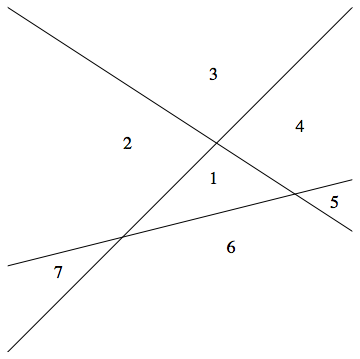
\includegraphics[width=0.6\linewidth]{images/exercise-8-2-3.png}
\caption*{\textbf{Figure 8.2.3:} A general configuration of three lines}
\end{figure}
\par\smallskip%
\noindent\textbf{Answer}.\quad%
\hypertarget{p-2607}{}%
Imagine drawing line \(k\) in one of the infinite regions that it passes through. That infinite region is divided into two infinite regions by line \(k\). As line \(k\) is drawn through every one of the \(k-1\) previous lines, you enter another region that line \(k\) divides. Therefore \(k\) regions are divided and the number of regions is increased by \(k\).  From this observation we get \(P(5)=16\).%
\end{divisionsolution}%
\begin{divisionsolution}{8.2.3.4}{}{exercise-317}%
\hypertarget{p-2608}{}%
A sample of a radioactive substance is expected to decay by 0.15 percent each hour. If \(w_t,\) \(t \geq  0\), is the weight of the sample \(t\) hours into an experiment, write a recurrence relation for \(w\).%
\end{divisionsolution}%
\begin{divisionsolution}{8.2.3.5}{}{exercise-318}%
\hypertarget{p-2609}{}%
Let \(M(n)\) be the number of multiplications needed to evaluate an \(n^{th}\) degree polynomial. Use the recursive definition of a polynomial expression to define \(M\) recursively.%
\par\smallskip%
\noindent\textbf{Answer}.\quad%
\hypertarget{p-2610}{}%
For \(n\) greater than zero, \(M(n)=M(n-1)+1\), and \(M(0)=0\).%
\end{divisionsolution}%
\section*{8.3 Recurrence Relations}
\addcontentsline{toc}{section}{8.3 Recurrence Relations}
\sectionmark{8.3 Recurrence Relations}
\subsection*{8.3.5 Exercises for Section 8.3}
\addcontentsline{toc}{subsection}{8.3.5 Exercises for Section 8.3}
\hypertarget{p-2709}{}%
Solve the following sets of recurrence relations and initial conditions:%
\begin{exercisegroup}
\begin{divisionsolutioneg}{8.3.5.1}{}{exercise-319}%
\hypertarget{p-2710}{}%
\(S(k) - 10S(k - 1) + 9S(k - 2) = 0\), \(S(0) = 3\), \(S(1) = 11\)%
\par\smallskip%
\noindent\textbf{Answer}.\quad%
\hypertarget{p-2711}{}%
\(S(k)=2+9^k\)%
\end{divisionsolutioneg}%
\begin{divisionsolutioneg}{8.3.5.2}{}{exercise-320}%
\hypertarget{p-2712}{}%
\(S(k) - 9S(k - 1) + 18S(k - 2) = 0\), \(S(0) = 0\), \(S(1) = 3\)%
\end{divisionsolutioneg}%
\begin{divisionsolutioneg}{8.3.5.3}{}{exercise-321}%
\hypertarget{p-2713}{}%
\(S(k) - 0.25S(k - 1) = 0\), \(S(0) = 6\)%
\par\smallskip%
\noindent\textbf{Answer}.\quad%
\hypertarget{p-2714}{}%
\(S(k)=6(1/4)^k\)%
\end{divisionsolutioneg}%
\begin{divisionsolutioneg}{8.3.5.4}{}{exercise-322}%
\hypertarget{p-2715}{}%
\(S(k) - 20S(k - 1) + 100S(k - 2) = 0\), \(S(0) = 2\), \(S(1) = 50\)%
\end{divisionsolutioneg}%
\begin{divisionsolutioneg}{8.3.5.5}{}{exercise-323}%
\hypertarget{p-2716}{}%
\(S(k) - 2S(k - 1) + S(k - 2) = 2 \textrm{,  }S(0) = 25,\textrm{  }S(1) = 16\)%
\par\smallskip%
\noindent\textbf{Answer}.\quad%
\hypertarget{p-2717}{}%
\(S(k)=k^2-10k+25\)%
\end{divisionsolutioneg}%
\begin{divisionsolutioneg}{8.3.5.6}{}{exercise-324}%
\hypertarget{p-2718}{}%
\(S(k) - S(k - 1) - 6S(k - 2) = -30\), \(S(0) = 7\), \(S(1) = 10\)%
\end{divisionsolutioneg}%
\begin{divisionsolutioneg}{8.3.5.7}{}{exercise-325}%
\hypertarget{p-2719}{}%
\(S(k) - 5S (k - 1) = 5^k,\textrm{  }S(0) = 3\)%
\par\smallskip%
\noindent\textbf{Answer}.\quad%
\hypertarget{p-2720}{}%
\(S(k)=(3+k)5^k\)%
\end{divisionsolutioneg}%
\begin{divisionsolutioneg}{8.3.5.8}{}{exercise-326}%
\hypertarget{p-2721}{}%
\(S(k) - 5S(k - 1) + 6S(k - 2) = 2,\textrm{  }S(0) = -1,\textrm{  }S(1) = 0\)%
\end{divisionsolutioneg}%
\begin{divisionsolutioneg}{8.3.5.9}{}{exercise-327}%
\hypertarget{p-2722}{}%
\(S(k) - 4S(k - 1) + 4S(k - 2) = 3k + 2^k \textrm{,  }S(0) = 1, S(1) = 1\)%
\par\smallskip%
\noindent\textbf{Answer}.\quad%
\hypertarget{p-2723}{}%
\(S(k)=(12+3k)+\left(k^2+7k-22\right)2^{k-1}\)%
\end{divisionsolutioneg}%
\begin{divisionsolutioneg}{8.3.5.10}{}{exercise-328}%
\hypertarget{p-2724}{}%
\(S(k) = r S(k - 1) + a\), \(S(0) = 0\), \(r, a \geq  0, r \neq  1\)%
\end{divisionsolutioneg}%
\begin{divisionsolutioneg}{8.3.5.11}{}{exercise-329}%
\hypertarget{p-2725}{}%
\(S(k) - 4S(k - 1) - 11S(k- 2)+ 30S(k - 3) = 0\), \(S(0) = 0\),\(S(1) = -35,\textrm{  }S(2) = -85\)%
\par\smallskip%
\noindent\textbf{Answer}.\quad%
\hypertarget{p-2726}{}%
\(P(k)=4(-3)^k+2^k-5^{k+1}\)%
\end{divisionsolutioneg}%
\end{exercisegroup}
\par\medskip\noindent
\begin{divisionsolution}{8.3.5.12}{}{exercise-330}%
\hypertarget{p-2727}{}%
Find a closed form expression for \(P(k)\) in Exercise 3 of Section 8.2.%
\end{divisionsolution}%
\begin{divisionsolution}{8.3.5.13}{}{exercise-331}%
\hypertarget{p-2728}{}%
\leavevmode%
\begin{enumerate}[label=(\alph*)]
\item\hypertarget{li-1348}{}\hypertarget{p-2729}{}%
Find a closed form expression for the terms of the Fibonacci sequence (see Example~8.1.8).%
\item\hypertarget{li-1349}{}\hypertarget{p-2730}{}%
The sequence \(C\) was defined by \(C_r\) = the number of strings of zeros and ones with length \(r\) having no consecutive zeros (Example~8.2.2(c)). Its recurrence relation is the same as that of the Fibonacci sequence. Determine a closed form expression for \(C_r\), \(r \geq  1\).%
\end{enumerate}
%
\par\smallskip%
\noindent\textbf{Answer}.\quad%
\hypertarget{p-2731}{}%
\leavevmode%
\begin{enumerate}[label=(\alph*)]
\item\hypertarget{li-1350}{}\hypertarget{p-2732}{}%
The characteristic equation is \(a^2-a-1=0\), which has solutions \(\alpha =\left.\left(1+\sqrt{5}\right)\right/2\) and \(\beta =\left.\left(1-\sqrt{5}\right)\right/2\), It is useful to point out that \(\alpha +\beta =1\) and \(\alpha -\beta =\sqrt{5}\). The general solution is \(F(k)=b_1\alpha ^k+b_2\beta ^k\). Using the initial conditions, we obtain the system: \(b_1+b_2=1\) and \(b_1\alpha +b_2\beta =1\). The solution to this system is \(b_1=\alpha /(\alpha -\beta )=\left.\left(5+\sqrt{5}\right)\right/2\sqrt{5}\) and  \(b_2=\beta /(\alpha -\beta )=\left.\left(5-\sqrt{5}\right)\right/2\sqrt{5}\)%
\par
\hypertarget{p-2733}{}%
Therefore the final solution is%
\begin{equation*}
\begin{split}
F(n) & = \frac{\alpha^{n+1}-\beta^{n+1}}{\alpha-\beta} \\
& = \frac{\left(\left.\left(1+\sqrt{5}\right)\right/2\right)^{n+1}
-\left(\left.\left(1-\sqrt{5}\right)\right/2\right)^{n+1}}{\sqrt{5}}\\
\end{split}
\end{equation*}
%
\item\hypertarget{li-1351}{}\hypertarget{p-2734}{}%
\(C_r=F(r+1)\)%
\end{enumerate}
%
\end{divisionsolution}%
\begin{divisionsolution}{8.3.5.14}{}{exercise-332}%
\hypertarget{p-2735}{}%
If \(S(n)=\sum_{j=1}^n g(j)\),\(n\geq 1\), then \(S\) can be described with the recurrence relation \(S(n) = S(n-1) + g(n)\). For each of the following sequences that are defined using a summation, find a closed form expression:%
\par
\hypertarget{p-2736}{}%
\leavevmode%
\begin{enumerate}[label=(\alph*)]
\item\hypertarget{li-1352}{}\hypertarget{p-2737}{}%
\(S(n) =\sum_{j=1}^n j\), \(n\geq 1\)%
\item\hypertarget{li-1353}{}\hypertarget{p-2738}{}%
\(Q(n) = \sum_{j=1}^n j^2\), \(n\geq 1\)%
\item\hypertarget{li-1354}{}\hypertarget{p-2739}{}%
\(P(n) =\)\(\sum_{j=1}^n \left(\frac{1}{2}\right)^j\), \(n\geq 0\)%
\item\hypertarget{li-1355}{}\hypertarget{p-2740}{}%
\(T(n)= \sum_{j=1}^n j^3\), \(n\geq 1\)%
\end{enumerate}
%
\end{divisionsolution}%
\begin{divisionsolution}{8.3.5.15}{}{exercise-333}%
\hypertarget{p-2741}{}%
Let \(D(n)\) be the number of ways that the set \(\{1, 2, . . . , n\}\), \(n \geq  1\), can be partitioned into two nonempty subsets.%
\par
\hypertarget{p-2742}{}%
\leavevmode%
\begin{enumerate}[label=(\alph*)]
\item\hypertarget{li-1356}{}\hypertarget{p-2743}{}%
Find a recurrence relation for \(D\). (Hint: It will be a first-order linear relation.)%
\item\hypertarget{li-1357}{}\hypertarget{p-2744}{}%
Solve the recurrence relation.%
\end{enumerate}
%
\par\smallskip%
\noindent\textbf{Answer}.\quad%
\hypertarget{p-2745}{}%
\leavevmode%
\begin{enumerate}[label=(\alph*)]
\item\hypertarget{li-1358}{}\hypertarget{p-2746}{}%
For each two-block partition of \(\{1,2,\dots, n-1\}\), there are two partitions we can create when we add \(n\), but there is one additional two-block partition to count for which one block is \(\{n\}\).  Therefore,  \(D(n)=2D(n-1)+1 \textrm{ for } n \geq 2 \textrm{ and } D(1)=0.\)%
\item\hypertarget{li-1359}{}\hypertarget{p-2747}{}%
\(D(n)=2^{n-1}-1\)%
\end{enumerate}
%
\end{divisionsolution}%
\begin{divisionsolution}{8.3.5.16}{}{exercise-334}%
\hypertarget{p-2748}{}%
If you were to deposit a certain amount of money at the end of each year for a number of years, this sequence of payments would be called an annuity (see Example~8.3.21).\leavevmode%
\begin{enumerate}[label=(\alph*)]
\item\hypertarget{li-1360}{}\hypertarget{p-2749}{}%
Find a closed form expression for the balance or value of an annuity that consists of payments of \(q\) dollars at a rate of interest of \(i\). Note that for a normal annuity, the first payment is made after one year.%
\item\hypertarget{li-1361}{}\hypertarget{p-2750}{}%
With an interest rate of 5.5 percent, how much would you need to deposit into an annuity to have a value of one million dollars after 18 years?%
\item\hypertarget{li-1362}{}\hypertarget{p-2751}{}%
The payment of a loan is a form of annuity in which the initial value is some negative amount (the amount of the loan) and the annuity ends when the value is raised to zero. How much could you borrow if you can afford to pay \textdollar{}5,000 per year for 25 years at 11 percent interest?%
\end{enumerate}
%
\end{divisionsolution}%
\begin{divisionsolution}{8.3.5.17}{}{exercise-335}%
\hypertarget{p-2752}{}%
Suppose that \(C\) is a small positive number. Consider the recurrence relation \(B(k) - 2B(k - 1) + \left(1 - C ^2\right)B(k - 2)
= C^2\), with initial conditions \(B(0) = 1\) and \(B(1) = 1\). If \(C\) is small enough, we might consider approximating the relation by replacing \(1 - C^2\) with 1 and \(C^2\) with 0. Solve the original relation and its approximation. Let \(B_a\) a be the solution of the approximation. Compare closed form expressions for \(B(k)\) and \(B_a(k)\). Their forms are very different because the characteristic roots of the original relation were close together and the approximation resulted in one double characteristic root.If characteristic roots of a relation are relatively far apart, this problem will not occur. For example, compare the general solutions of \(S(k) + 1.001S(k - 1) - 2.004002 S(k - 2) = 0.0001\) and \(S_a(k) + S_a(k - 1) - 2S_a(k - 2) = 0\).%
\end{divisionsolution}%
\section*{8.4 Some Common Recurrence Relations}
\addcontentsline{toc}{section}{8.4 Some Common Recurrence Relations}
\sectionmark{8.4 Some Common Recurrence Relations}
\subsection*{8.4.5 Exercises for Section 8.4}
\addcontentsline{toc}{subsection}{8.4.5 Exercises for Section 8.4}
\begin{divisionsolution}{8.4.5.1}{}{exercise-336}%
\hypertarget{p-2800}{}%
Solve the following recurrence relations. Indicate whether your solution is an improvement over iteration.%
\par
\hypertarget{p-2801}{}%
\leavevmode%
\begin{enumerate}[label=(\alph*)]
\item\hypertarget{li-1368}{}\hypertarget{p-2802}{}%
\(n S(n) - S(n - 1) = 0\), \(S(0) = 1\).%
\item\hypertarget{li-1369}{}\hypertarget{p-2803}{}%
\(T(k) + 3k T(k - 1) = 0\), \(T(0) = 1\).%
\item\hypertarget{li-1370}{}\hypertarget{p-2804}{}%
\(U(k) -\frac{k-1}{k}U(k - 1) = 0\), \(k \geq  2\), \(U(1) = 1\).%
\end{enumerate}
%
\par\smallskip%
\noindent\textbf{Answer}.\quad%
\hypertarget{p-2805}{}%
\leavevmode%
\begin{enumerate}[label=(\alph*)]
\item\hypertarget{li-1371}{}\hypertarget{p-2806}{}%
\(S(n)=1/n\)!%
\item\hypertarget{li-1372}{}\hypertarget{p-2807}{}%
\(U(k)=1/k\), an improvement.%
\item\hypertarget{li-1373}{}\hypertarget{p-2808}{}%
\(T(k)=(-3)^kk\)!, no improvement.%
\end{enumerate}
%
\end{divisionsolution}%
\begin{divisionsolution}{8.4.5.2}{}{exercise-337}%
\hypertarget{p-2809}{}%
Prove that if \(n \geq 0\), \(\lfloor n/2\rfloor +\lceil n/2\rceil = n\). (Hint: Consider the cases of \(n\) odd and \(n\) even separately.)%
\end{divisionsolution}%
\begin{divisionsolution}{8.4.5.3}{}{exercise-338}%
\hypertarget{p-2810}{}%
Solve as completely as possible:%
\par
\hypertarget{p-2811}{}%
\leavevmode%
\begin{enumerate}[label=(\alph*)]
\item\hypertarget{li-1374}{}\hypertarget{p-2812}{}%
\(T(n) = 3 + T(\lfloor n/2\rfloor )\), \(T(0) = 0\).%
\item\hypertarget{li-1375}{}\hypertarget{p-2813}{}%
\(T(n) = 1 + \frac{1}{2}T(\lfloor n/2\rfloor )\), \(T(0) = 2\).%
\item\hypertarget{li-1376}{}\hypertarget{p-2814}{}%
\(V(n) = 1 + V\lfloor n/8\rfloor )\), \(V(0) = 0\). (Hint: Write \(n\) in octal form.)%
\end{enumerate}
%
\par\smallskip%
\noindent\textbf{Answer}.\quad%
\hypertarget{p-2815}{}%
\leavevmode%
\begin{enumerate}[label=(\alph*)]
\item\hypertarget{li-1377}{}\hypertarget{p-2816}{}%
\(T(n)=3\left(\left\lfloor \log_2n\right\rfloor +1\right)\)%
\item\hypertarget{li-1378}{}\hypertarget{p-2817}{}%
\(T(n)=2\)%
\item\hypertarget{li-1379}{}\hypertarget{p-2818}{}%
\(V(n)=\left\lfloor \log_8n\right\rfloor +1\)%
\end{enumerate}
%
\end{divisionsolution}%
\begin{divisionsolution}{8.4.5.4}{}{exercise-339}%
\hypertarget{p-2819}{}%
Prove by induction that if \(T(n)= 1 + T (\lfloor n/2 \rfloor )\), \(T(0) = 0\), and \(2^{r-1}\leq n < 2^r\) , \(r \geq  1\), then \(T(n) = r\).%
\par\smallskip%
\noindent\textbf{Hint}.\quad%
\hypertarget{p-2820}{}%
Prove by induction on \(r\).%
\end{divisionsolution}%
\begin{divisionsolution}{8.4.5.5}{}{exercise-340}%
\hypertarget{p-2821}{}%
Use the substitution \(S(n) = T(n+1)/T(n)\)  to solve \(T(n)T(n-2)=T(n-1)^2\) for \(n \geq  2\), with \(T(0) = 1\), \(T(1) = 6\), and \(T(n) \geq  0\).%
\par\smallskip%
\noindent\textbf{Answer}.\quad%
\hypertarget{p-2822}{}%
The indicated substitution yields \(S(n)=S(n+1)\). Since \(S(0)=T(1)/T(0)=6\), \(S(n)=6\) for all \(n\). Therefore \(T(n+1)=6T(n)\Rightarrow T(n)=6^n\).%
\end{divisionsolution}%
\begin{divisionsolution}{8.4.5.6}{}{exercise-341}%
\hypertarget{p-2823}{}%
Use the substitution \(G(n) =T(n)^2\) to solve \(T(n)^2-T(n-1)^2=1\) for \(n \geq  1\), with \(T(0) = 10\).%
\end{divisionsolution}%
\begin{divisionsolution}{8.4.5.7}{}{exercise-342}%
\hypertarget{p-2824}{}%
Solve as completely as possible:%
\par
\hypertarget{p-2825}{}%
\leavevmode%
\begin{enumerate}[label=(\alph*)]
\item\hypertarget{li-1380}{}\hypertarget{p-2826}{}%
\(Q(n)=1+Q\left(\left\lfloor \sqrt{n}\right\rfloor \right)\), \(n \geq  2\), \(Q(1) = 0\).%
\item\hypertarget{li-1381}{}\hypertarget{p-2827}{}%
\(R(n)=n +R(\lfloor n/2\rfloor )\), \(n \geq  1\), \(R(0) = 0\).%
\end{enumerate}
%
\par\smallskip%
\noindent\textbf{Answer}.\quad%
\hypertarget{p-2828}{}%
\leavevmode%
\begin{enumerate}[label=(\alph*)]
\item\hypertarget{li-1382}{}\hypertarget{p-2829}{}%
A good approximation to the solution of this recurrence relation is based on the following observation: \(n\) is a power of a power of two; that is, \(n\) is \(2^m\), where \(m=2^k\) , then \(Q(n)=1+Q\left(2^{m/2}\right)\). By applying this recurrence relation \(k\) times we obtain \(Q(n)=k\). Going back to the original form of \(n\), \(\log _2n=2^k\) or \(\log _2\left(\log _2n\right)=k\). We would expect that in general, \(Q(n)\) is \(\left\lfloor \log _2\left(\log _2n\right)\right\rfloor\). We do not see any elementary method for arriving at an exact solution.%
\item\hypertarget{li-1383}{}\hypertarget{p-2830}{}%
Suppose that \(n\) is a positive integer with \(2^{k-1} \leq n < 2^k\). Then \(n\) can be written in binary form, \(\left(a_{k-1}a_{k-2}\cdots  a_2a_1a_0\right)_{\textrm{two}}\) with \(a_{k-1}=1\) and \(R(n)\) is equal to the sum \(\underset{i=0}{\overset{k-1}{\Sigma }}\) \(\left(a_{k-1}a_{k-2}\cdots  a_i\right)_{\textrm{two}}\). If \(2^{k-1}\leq n < 2^k\), then we can estimate this sum to be between \(2n-1\) and \(2n+1\). Therefore, \(R(n)\approx 2n\).%
\end{enumerate}
%
\end{divisionsolution}%
\begin{divisionsolution}{8.4.5.8}{}{exercise-343}%
\hypertarget{p-2831}{}%
Suppose Step 1 of the merge sort algorithm did take a significant amount of time. Assume it takes 0.1 time unit, independent of the value of \(n\).%
\par
\hypertarget{p-2832}{}%
\leavevmode%
\begin{enumerate}[label=(\alph*)]
\item\hypertarget{li-1384}{}\hypertarget{p-2833}{}%
Write out a new recurrence relation for \(T(n)\) that takes this factor into account.%
\item\hypertarget{li-1385}{}\hypertarget{p-2834}{}%
Solve for \(T\left(2^r\right)\), \(r \geq  0\).%
\item\hypertarget{li-1386}{}\hypertarget{p-2835}{}%
Assuming the solution for powers of 2 is a good estimate for all \(n\), compare your result to the solution in the text. As gets large, is there really much difference?%
\end{enumerate}
%
\end{divisionsolution}%
\section*{8.5 Generating Functions}
\addcontentsline{toc}{section}{8.5 Generating Functions}
\sectionmark{8.5 Generating Functions}
\subsection*{8.5.7 Exercises for Section 8.5}
\addcontentsline{toc}{subsection}{8.5.7 Exercises for Section 8.5}
\begin{divisionsolution}{8.5.7.1}{}{exercise-344}%
\hypertarget{p-2950}{}%
What sequences have the following generating functions?%
\par
\hypertarget{p-2951}{}%
\leavevmode%
\begin{enumerate}[label=(\alph*)]
\item\hypertarget{li-1437}{}\hypertarget{p-2952}{}%
1%
\item\hypertarget{li-1438}{}\hypertarget{p-2953}{}%
\(\frac{10}{2-z}\)%
\item\hypertarget{li-1439}{}\hypertarget{p-2954}{}%
\(1 + z\)%
\item\hypertarget{li-1440}{}\hypertarget{p-2955}{}%
\(\frac{3}{1+2z}+ \frac{3}{1-3z}\)%
\end{enumerate}
%
\par\smallskip%
\noindent\textbf{Answer}.\quad%
\hypertarget{p-2956}{}%
\leavevmode%
\begin{enumerate}[label=(\alph*)]
\item\hypertarget{li-1441}{}\hypertarget{p-2957}{}%
\(1,0,0,0,0,\ldots\)%
\item\hypertarget{li-1442}{}\hypertarget{p-2958}{}%
\(5(1/2)^k\)%
\item\hypertarget{li-1443}{}\hypertarget{p-2959}{}%
\(1,1,0,0,0,\ldots\)%
\item\hypertarget{li-1444}{}\hypertarget{p-2960}{}%
\(3(-2)^k+3\cdot 3^k\)%
\end{enumerate}
%
\end{divisionsolution}%
\begin{divisionsolution}{8.5.7.2}{}{exercise-345}%
\hypertarget{p-2961}{}%
What sequences have the following generating functions?%
\par
\hypertarget{p-2962}{}%
\leavevmode%
\begin{enumerate}[label=(\alph*)]
\item\hypertarget{li-1445}{}\hypertarget{p-2963}{}%
\(\frac{1}{1+z}\)%
\item\hypertarget{li-1446}{}\hypertarget{p-2964}{}%
\(\frac{1}{4-3z}\)%
\item\hypertarget{li-1447}{}\hypertarget{p-2965}{}%
\(\frac{2}{1-z}+ \frac{1}{1+z}\)%
\item\hypertarget{li-1448}{}\hypertarget{p-2966}{}%
\(\frac{z+2}{z+3}\)%
\end{enumerate}
%
\end{divisionsolution}%
\begin{divisionsolution}{8.5.7.3}{}{exercise-346}%
\hypertarget{p-2967}{}%
Find closed form expressions for the generating functions of the following sequences:%
\par
\hypertarget{p-2968}{}%
\leavevmode%
\begin{enumerate}[label=(\alph*)]
\item\hypertarget{li-1449}{}\hypertarget{p-2969}{}%
\(V(n) = 9^n\)%
\item\hypertarget{li-1450}{}\hypertarget{p-2970}{}%
\(P\), where \(P(k) - 6 P(k - 1) + 5 P(k - 2) = 0\) for \(k \geq  2\), with \(P(0) = 2\) and \(P(1) = 2\).%
\item\hypertarget{li-1451}{}\hypertarget{p-2971}{}%
The Fibonacci sequence: \(F(k + 2) = F(k + 1) + F(k)\), \(k \geq  0\), with \(F(0) = F(1) = 1\).%
\end{enumerate}
%
\par\smallskip%
\noindent\textbf{Answer}.\quad%
\hypertarget{p-2972}{}%
\leavevmode%
\begin{enumerate}[label=(\alph*)]
\item\hypertarget{li-1452}{}\hypertarget{p-2973}{}%
\(1/(1-9z)\)%
\item\hypertarget{li-1453}{}\hypertarget{p-2974}{}%
\((2-10z)\left/\left(1-6z+5z^2\right)\right.\)%
\item\hypertarget{li-1454}{}\hypertarget{p-2975}{}%
\(1\left/\left(1-z-z^2\right)\right.\)%
\end{enumerate}
%
\end{divisionsolution}%
\begin{divisionsolution}{8.5.7.4}{}{exercise-347}%
\hypertarget{p-2976}{}%
Find closed form expressions for the generating functions of the following sequences:%
\par
\hypertarget{p-2977}{}%
\leavevmode%
\begin{enumerate}[label=(\alph*)]
\item\hypertarget{li-1455}{}\hypertarget{p-2978}{}%
\(W(n) = \binom{5}{n} 2^n\) for \(0 \leq  n \leq  5\) and \(W(n) = 0\) for \(n > 5\).%
\item\hypertarget{li-1456}{}\hypertarget{p-2979}{}%
\(Q\), where \(Q(k) + Q(k - 1) - 42Q(k - 2) = 0\) for \(k\geq 2\), with \(Q(0) = 2\) and \(Q(1) = 2\).%
\item\hypertarget{li-1457}{}\hypertarget{p-2980}{}%
\(G\), where \(G(k + 3) = G(k + 2) + G(k + 1) + G(k)\) for \(k \geq  0\), with \(G(0) = G(1) = G(2) = 1\).%
\end{enumerate}
%
\end{divisionsolution}%
\begin{divisionsolution}{8.5.7.5}{}{exercise-348}%
\hypertarget{p-2981}{}%
For each of the following expressions, find the partial fraction decomposition and identify the sequence having the expression as a generating function.%
\par
\hypertarget{p-2982}{}%
\leavevmode%
\begin{enumerate}[label=(\alph*)]
\item\hypertarget{li-1458}{}\hypertarget{p-2983}{}%
\(\frac{5+2z}{1-4z^2}\)%
\item\hypertarget{li-1459}{}\hypertarget{p-2984}{}%
\(\frac{32-22z}{2-3z+z^2}\)%
\item\hypertarget{li-1460}{}\hypertarget{p-2985}{}%
\(\frac{6-29z}{1-11z+ 30z^2}\)%
\end{enumerate}
%
\par\smallskip%
\noindent\textbf{Answer}.\quad%
\hypertarget{p-2986}{}%
\leavevmode%
\begin{enumerate}[label=(\alph*)]
\item\hypertarget{li-1461}{}\hypertarget{p-2987}{}%
\(3/(1-2z)+2/(1+2z), 3\cdot 2^k+2(-2)^k\)%
\item\hypertarget{li-1462}{}\hypertarget{p-2988}{}%
\(10/(1-z)+12/(2-z), 10+6(1/2)^k\)%
\item\hypertarget{li-1463}{}\hypertarget{p-2989}{}%
\(-1/(1-5z)+7/(1-6z), 7\cdot 6^k-5^k\)%
\end{enumerate}
%
\end{divisionsolution}%
\begin{divisionsolution}{8.5.7.6}{}{exercise-349}%
\hypertarget{p-2990}{}%
Find the partial fraction decompositions and identify the sequence having the following expressions:%
\par
\hypertarget{p-2991}{}%
\leavevmode%
\begin{enumerate}[label=(\alph*)]
\item\hypertarget{li-1464}{}\hypertarget{p-2992}{}%
\(\frac{1}{1-9z^2}\)%
\item\hypertarget{li-1465}{}\hypertarget{p-2993}{}%
\(\frac{1+3z}{16-8z+z^2}\)%
\item\hypertarget{li-1466}{}\hypertarget{p-2994}{}%
\(\frac{2z}{1-6z-7z^2}\)%
\end{enumerate}
%
\end{divisionsolution}%
\begin{divisionsolution}{8.5.7.7}{}{exercise-350}%
\hypertarget{p-2995}{}%
Given that \(S(k) = k\) and \(T(k) = 10k\), what is the \(k^{\text{th}}\) term of the generating function of each of the following sequences:%
\par
\hypertarget{p-2996}{}%
\leavevmode%
\begin{enumerate}[label=(\alph*)]
\item\hypertarget{li-1467}{}\hypertarget{p-2997}{}%
\(S + T\)%
\item\hypertarget{li-1468}{}\hypertarget{p-2998}{}%
\(S\uparrow  * T\)%
\item\hypertarget{li-1469}{}\hypertarget{p-2999}{}%
\(S * T\)%
\item\hypertarget{li-1470}{}\hypertarget{p-3000}{}%
\(S\uparrow *S\uparrow\)%
\end{enumerate}
%
\par\smallskip%
\noindent\textbf{Answer}.\quad%
\hypertarget{p-3001}{}%
\leavevmode%
\begin{enumerate}[label=(\alph*)]
\item\hypertarget{li-1471}{}\hypertarget{p-3002}{}%
\(11k\)%
\item\hypertarget{li-1472}{}\hypertarget{p-3003}{}%
\((5/3)k(k+1)(2k+1)+5k(k+1)\)%
\item\hypertarget{li-1473}{}\(\underset{j=0}{\overset{k}{\Sigma }}(j)(10(k-j))=10k\underset{j=0}{\overset{k}{\Sigma }}j-10\underset{j=0}{\overset{k}{\Sigma }}j^2\) \(=5k^2(k+1)-(5k(k+1)(2k+1)/6)
=(5/3)k(k+1)(2k+1)\)%
\item\hypertarget{li-1474}{}\hypertarget{p-3004}{}%
\(k(k+1)(2k+7)/12\)%
\end{enumerate}
%
\end{divisionsolution}%
\begin{divisionsolution}{8.5.7.8}{}{exercise-351}%
\hypertarget{p-3005}{}%
Given that \(P(k) = \binom{10}{k}\) and \(Q(k) = k!\), what is the \(k^{\text{th}}\) term of the generating function of each of the following sequences:%
\par
\hypertarget{p-3006}{}%
\leavevmode%
\begin{enumerate}[label=(\alph*)]
\item\hypertarget{li-1475}{}\hypertarget{p-3007}{}%
\(P * P\)%
\item\hypertarget{li-1476}{}\hypertarget{p-3008}{}%
\(P + P\uparrow\)%
\item\hypertarget{li-1477}{}\hypertarget{p-3009}{}%
\(P * Q\)%
\item\hypertarget{li-1478}{}\hypertarget{p-3010}{}%
\(Q * Q\)%
\end{enumerate}
%
\end{divisionsolution}%
\begin{divisionsolution}{8.5.7.9}{}{exercise-352}%
\hypertarget{p-3011}{}%
A game is played by rolling a die five times. For the \(k^{\text{th}}\) roll, one point is added to your score if you roll a number higher than \(k\). Otherwise, your score is zero for that roll. For example, the sequence of rolls \(2,3,4,1,2\) gives you a total score of three; while a sequence of 1,2,3,4,5 gives you a score of zero. Of the \(6^5 = 7776\) possible sequences of rolls, how many give you a score of zero?, of one? \(\ldots \) of five?%
\par\smallskip%
\noindent\textbf{Answer}.\quad%
\hypertarget{p-3012}{}%
Coefficients of \(z^0\) through \(z^5\) in \((1+5z)(2+4z)(3+3z)(4+2z)(5+z)\)%
\par
\hypertarget{p-3013}{}%
\(\begin{array}{cc}
k & \textrm{ Number of ways of getting a score of } k \\
0 & 120 \\
1 & 1044 \\
2 & 2724 \\
3 & 2724 \\
4 & 1044 \\
5 & 120 \\
\end{array}\)%
\end{divisionsolution}%
\begin{divisionsolution}{8.5.7.10}{}{exercise-353}%
\hypertarget{p-3014}{}%
Suppose that you roll a die ten times in a row and record the square of each number that you roll. How many ways could the sum of the squares of your rolls equal 40? What is the most common outcome?%
\end{divisionsolution}%
\chapter*{9 Graph Theory}
\addcontentsline{toc}{chapter}{9 Graph Theory}
\chaptermark{9 Graph Theory}
\section*{9.1 Graphs - General Introduction}
\addcontentsline{toc}{section}{9.1 Graphs - General Introduction}
\sectionmark{9.1 Graphs - General Introduction}
\subsection*{9.1.5 Exercises for Section 9.1}
\addcontentsline{toc}{subsection}{9.1.5 Exercises for Section 9.1}
\begin{divisionsolution}{9.1.5.1}{}{exercise-354}%
\hypertarget{p-3072}{}%
What is the significance of the fact that there is a path connecting vertex \(b\) with every other vertex in Figure~9.1.10, as it applies to various situations that it models?%
\par\smallskip%
\noindent\textbf{Answer}.\quad%
\hypertarget{p-3073}{}%
In Figure~9.1.10, computer \(b\) can communicate with all other computers. In Figure~9.1.11, there are direct roads to and from city \(b\) to all other cities.%
\end{divisionsolution}%
\begin{divisionsolution}{9.1.5.2}{}{exercise-355}%
\hypertarget{p-3074}{}%
Draw a graph similar to Figure~9.1.4 that represents the set of strings of 0's and 1's containing no more than two consecutive 1's in any part of the string.%
\end{divisionsolution}%
\begin{divisionsolution}{9.1.5.3}{}{exercise-356}%
\hypertarget{p-3075}{}%
Draw a directed graph that models the set of strings of 0's and 1's (zero or more of each) where all of the 1's must appear consecutively.%
\par\smallskip%
\noindent\textbf{Answer}.\quad%
\leavevmode%
\begin{figure}
\centering
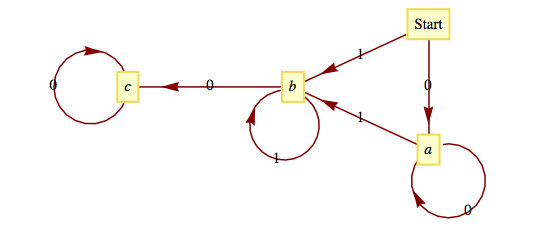
\includegraphics[width=0.75\linewidth]{images/fig-sol-9-1-3.png}
\caption*{\textbf{Figure 9.1.36:} Solution to exercise 3 of Section 9.1}
\end{figure}
\end{divisionsolution}%
\begin{divisionsolution}{9.1.5.4}{}{exercise-357}%
\hypertarget{p-3076}{}%
In the NCAA final-four basketball tournament, the East champion plays the West champion, and the champions from the Mideast and Midwest play. The winners of the two games play for the national championship. Draw the eight different single-elimination tournament graphs that could occur.%
\end{divisionsolution}%
\begin{divisionsolution}{9.1.5.5}{}{exercise-358}%
\hypertarget{p-3077}{}%
What is the maximum number of edges in an undirected graph with eight vertices?%
\par\smallskip%
\noindent\textbf{Answer}.\quad%
\hypertarget{p-3078}{}%
The maximum number of edges would be \(\binom{8}{2} = \frac{(7)(8)}{2}=28\).%
\end{divisionsolution}%
\begin{divisionsolution}{9.1.5.6}{}{exercise-359}%
\hypertarget{p-3079}{}%
Which of the graphs in Figure~9.1.37 are isomorphic? What is the correspondence between their vertices?%
\begin{figure}
\centering
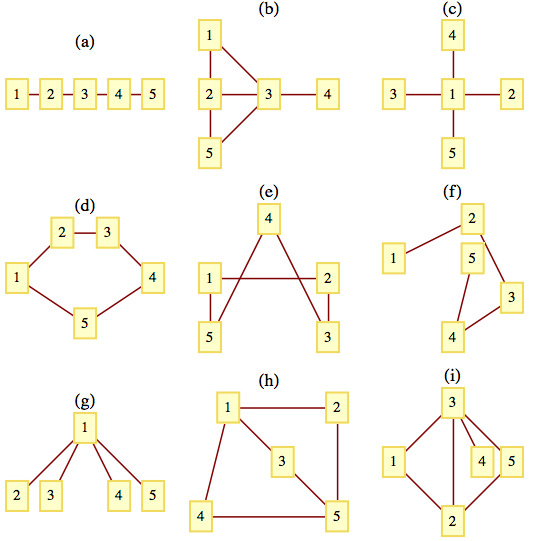
\includegraphics[width=1\linewidth]{images/fig-exercise-9-1-6.png}
\caption*{\textbf{Figure 9.1.37:} Which graphs are isomorphic to one another?}
\end{figure}
\end{divisionsolution}%
\begin{divisionsolution}{9.1.5.7}{}{exercise-360}%
\hypertarget{p-3080}{}%
\leavevmode%
\begin{enumerate}[label=(\alph*)]
\item\hypertarget{li-1491}{}\hypertarget{p-3081}{}%
How many edges does a complete tournament graph with \(n\) vertices have?%
\item\hypertarget{li-1492}{}\hypertarget{p-3082}{}%
How many edges does a single-elimination tournament graph with \(n\) vertices have?%
\end{enumerate}
%
\par\smallskip%
\noindent\textbf{Answer}.\quad%
\hypertarget{p-3083}{}%
\leavevmode%
\begin{enumerate}[label=(\alph*)]
\item\hypertarget{li-1493}{}\hypertarget{p-3084}{}%
\(\binom{n}{2}=\frac{(n-1)n}{2}\)%
\item\hypertarget{li-1494}{}\hypertarget{p-3085}{}%
\(n-1\), each vertex except the champion vertex has an indegree of 1 and the champion vertex has an indegree of zero.%
\end{enumerate}
%
\end{divisionsolution}%
\begin{divisionsolution}{9.1.5.8}{}{exercise-361}%
\hypertarget{p-3086}{}%
Draw complete undirected graphs with 1, 2, 3, 4, and 5 vertices. How many edges does a \(K_n\), a complete undirected graph with \(n\) vertices, have?%
\end{divisionsolution}%
\begin{divisionsolution}{9.1.5.9}{}{exercise-362}%
\hypertarget{p-3087}{}%
Determine whether the following sequences are graphic. Explain your logic.%
\par
\hypertarget{p-3088}{}%
\leavevmode%
\begin{enumerate}[label=(\alph*)]
\item\hypertarget{li-1495}{}\hypertarget{p-3089}{}%
\((6, 5, 4, 3, 2, 1, 0)\)%
\item\hypertarget{li-1496}{}\hypertarget{p-3090}{}%
\((2,2,2,2,2,2)\)%
\item\hypertarget{li-1497}{}\hypertarget{p-3091}{}%
\((3,2,2,2,2,2)\)%
\item\hypertarget{li-1498}{}\hypertarget{p-3092}{}%
\((5,3,3,3,3,3)\)%
\item\hypertarget{li-1499}{}\hypertarget{p-3093}{}%
\((1,1,1,1,1,1)\)%
\item\hypertarget{li-1500}{}\hypertarget{p-3094}{}%
\((5,5,4,3,2,1)\)%
\end{enumerate}
%
\par\smallskip%
\noindent\textbf{Answer}.\quad%
\hypertarget{p-3095}{}%
\leavevmode%
\begin{enumerate}[label=(\alph*)]
\item\hypertarget{li-1501}{}\hypertarget{p-3096}{}%
Not graphic - if the degree of a graph with seven vertices is 6, it is connected to all other vertices and so there cannot be a vertex with degree zero.%
\item\hypertarget{li-1502}{}\hypertarget{p-3097}{}%
Graphic.  One graph with this degree sequence is a cycle of length 6.%
\item\hypertarget{li-1503}{}\hypertarget{p-3098}{}%
Not Graphic. The number of vertices with odd degree is odd, which is impossible.%
\item\hypertarget{li-1504}{}\hypertarget{p-3099}{}%
Graphic.  A "wheel graph" with one vertex connected to all other and the others connected to one another in a cycle has this degree sequence.%
\item\hypertarget{li-1505}{}\hypertarget{p-3100}{}%
Graphic.  Pairs of vertices connected only to one another.%
\item\hypertarget{li-1506}{}\hypertarget{p-3101}{}%
Not Graphic.  With two vertices having maximal degree, 5, every vertex would need to have a degree of 2 or more, so the 1 in this sequence makes it non-graphic.%
\end{enumerate}
%
\end{divisionsolution}%
\begin{divisionsolution}{9.1.5.10}{}{exercise-363}%
\hypertarget{p-3102}{}%
\leavevmode%
\begin{enumerate}[label=(\alph*)]
\item\hypertarget{li-1507}{}\hypertarget{p-3103}{}%
Based on observations you might have made in exercise 9, describe as many characteristics as you can about graphic sequences of length \(n\).%
\item\hypertarget{li-1508}{}\hypertarget{p-3104}{}%
Consider the two graphs in Figure~9.1.38. Notice that they have the same degree sequences, \((2,2,2,2,2,2)\).  Explain why the two graphs are not isomorphic.%
\end{enumerate}
%
\begin{figure}
\centering
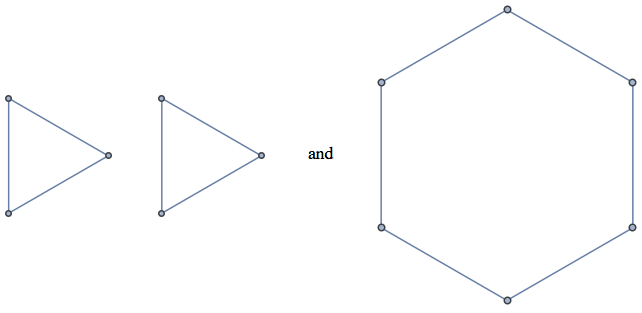
\includegraphics[width=1\linewidth]{images/fig-same-ds-9-1.png}
\caption*{\textbf{Figure 9.1.38:} Two graphs with the same degree sequences}
\end{figure}
\end{divisionsolution}%
\begin{divisionsolution}{9.1.5.11}{}{exercise-house-9-1}%
\hypertarget{p-3105}{}%
Draw a plan for the rooms of a house so that Figure~9.1.10 models connectedness of the rooms.  That is, \((a,b)\) is an edge if and only if a door connects rooms \(a\) and \(b\).%
\end{divisionsolution}%
\begin{divisionsolution}{9.1.5.12}{}{exercise-subgraphs}%
\hypertarget{p-3106}{}%
How many subgraphs are there of a \(K_n\), \(n \geq 1\).  How many of them are spanning graphs?%
\end{divisionsolution}%
\section*{9.2 Data Structures for Graphs}
\addcontentsline{toc}{section}{9.2 Data Structures for Graphs}
\sectionmark{9.2 Data Structures for Graphs}
\subsection*{9.2.3 Exercises for Section 9.2}
\addcontentsline{toc}{subsection}{9.2.3 Exercises for Section 9.2}
\begin{divisionsolution}{9.2.3.1}{}{exercise-366}%
\hypertarget{p-3129}{}%
Estimate the number of vertices and edges in each of the following graphs. Would the graph be considered sparse, so that an adjacency matrix would be inefficient?%
\par
\hypertarget{p-3130}{}%
\leavevmode%
\begin{enumerate}[label=(\alph*)]
\item\hypertarget{li-1512}{}\hypertarget{p-3131}{}%
Vertices: Cities of the world that are served by at least one airline. Edges: Pairs of cities that are connected by a regular direct flight.%
\item\hypertarget{li-1513}{}\hypertarget{p-3132}{}%
Vertices: ASCII characters. Edges: connect characters that differ in their binary code by exactly two bits.%
\item\hypertarget{li-1514}{}\hypertarget{p-3133}{}%
Vertices: All English words. Edges: An edge connects word \(x\) to word \(y\) if \(x\) is a prefix of \(y\).%
\end{enumerate}
%
\par\smallskip%
\noindent\textbf{Answer}.\quad%
\hypertarget{p-3134}{}%
\leavevmode%
\begin{enumerate}[label=(\alph*)]
\item\hypertarget{li-1515}{}\hypertarget{p-3135}{}%
A rough estimate of the number of vertices in the ``world airline graph'' would be the number of cities with population greater than or equal to 100,000. This is estimated to be around 4,100. There are many smaller cities that have airports, but some of the metropolitan areas with clusters of large cities are served by only a few airports.  4,000-5,000 is probably a good guess.   As for edges, that's a bit more difficult to estimate.  It's certainly not  a complete graph.  Looking at some medium sized airports such as Manchester, NH, the average number of cities that you can go to directly is in the 50-100 range.   So a very rough estimate would be   \(\frac{75 \cdot  4500}{2}=168,750\). This is far less than \(4,500^2\), so an edge list or dictionary of some kind would be more efficient.%
\item\hypertarget{li-1516}{}\hypertarget{p-3136}{}%
The number of ASCII characters is 128.  Each character would be connected to \(\binom{8}{2}=28\) others and so there are \(\frac{128 \dot 28}{2}=3,584\)  edges.  Comparing this to the \(128^2=16,384\), an array is probably the best choice.%
\item\hypertarget{li-1517}{}\hypertarget{p-3137}{}%
The Oxford English Dictionary as approximately a half-million words, although many are obsolete.   The number of edges is probably of the same order of magnitude as the number of words, so an edge list or dictionary is probably the best choice.%
\end{enumerate}
%
\end{divisionsolution}%
\begin{divisionsolution}{9.2.3.2}{}{exercise-367}%
\hypertarget{p-3138}{}%
Each edge of a graph is colored with one of the four colors red, blue, yellow, or green. How could you represent the edges in this graph using a variation of the adjacency matrix structure?%
\end{divisionsolution}%
\begin{divisionsolution}{9.2.3.3}{}{exercise-368}%
\hypertarget{p-3139}{}%
Directed graphs \(G_1, \dots, G_6\) , each with vertex set \(\{1,2,3,4,5\}\) are represented by the matrices below. Which graphs are isomorphic to one another?%
\par
\hypertarget{p-3140}{}%
\(G_1: \left(
\begin{array}{ccccc}
0 & 1 & 0 & 0 & 0 \\
0 & 0 & 1 & 0 & 0 \\
0 & 0 & 0 & 1 & 0 \\
0 & 0 & 0 & 0 & 1 \\
1 & 0 & 0 & 0 & 0 \\
\end{array}
\right)\)\(\quad \quad\)\(G_2: \left(
\begin{array}{ccccc}
0 & 0 & 0 & 0 & 0 \\
0 & 0 & 1 & 0 & 0 \\
0 & 0 & 0 & 0 & 0 \\
1 & 1 & 1 & 0 & 1 \\
0 & 0 & 0 & 0 & 0 \\
\end{array}
\right)\)\(\quad \quad\)\(G_3: \left(
\begin{array}{ccccc}
0 & 0 & 0 & 0 & 0 \\
1 & 0 & 0 & 0 & 1 \\
0 & 1 & 0 & 0 & 0 \\
0 & 0 & 1 & 0 & 0 \\
0 & 0 & 1 & 0 & 0 \\
\end{array}
\right)\) \(G_4: \left(
\begin{array}{ccccc}
0 & 1 & 1 & 1 & 1 \\
0 & 0 & 0 & 0 & 0 \\
0 & 0 & 0 & 0 & 0 \\
0 & 0 & 1 & 0 & 0 \\
0 & 0 & 0 & 0 & 0 \\
\end{array}
\right)\)\(\quad \quad\)\(\quad G_5: \left(
\begin{array}{ccccc}
0 & 0 & 0 & 0 & 1 \\
0 & 0 & 0 & 0 & 0 \\
0 & 1 & 0 & 1 & 0 \\
0 & 0 & 0 & 0 & 1 \\
0 & 0 & 1 & 0 & 0 \\
\end{array}
\right)\)\(\quad \quad\)\(G_6: \left(
\begin{array}{ccccc}
0 & 0 & 0 & 1 & 0 \\
0 & 0 & 0 & 0 & 0 \\
1 & 1 & 0 & 0 & 0 \\
0 & 0 & 1 & 0 & 0 \\
0 & 0 & 0 & 1 & 0 \\
\end{array}
\right)\)%
\par\smallskip%
\noindent\textbf{Answer}.\quad%
\hypertarget{p-3141}{}%
Each graph is isomorphic to itself. In addition, \(G_2 \text{ and } G_4\) are isomorphic; and \(G_3, G_5, \text{ and } G_6\) are isomorphic to one another.%
\end{divisionsolution}%
\begin{divisionsolution}{9.2.3.4}{}{exercise-369}%
\hypertarget{p-3142}{}%
The following Sage command verifies that the wheel graph with four vertices is isomorphic to the complete graph with four vertices.%
\begin{sageinput}
graphs.WheelGraph(4).is_isomorphic(graphs.CompleteGraph(4))
\end{sageinput}
\begin{sageoutput}
True
\end{sageoutput}
\hypertarget{p-3143}{}%
A list of all graphs in this the \mono{graphs} database is available via tab completion. Type "graphs." and then hit the tab key to see which graphs are available.  This can be done using the Sage application or SageMathCloud, but not sage cells.  Find some other pairs of isomorphic graphs in the database.%
\end{divisionsolution}%
\section*{9.3 Connectivity}
\addcontentsline{toc}{section}{9.3 Connectivity}
\sectionmark{9.3 Connectivity}
\subsection*{9.3.5 Exercises for Section 9.3}
\addcontentsline{toc}{subsection}{9.3.5 Exercises for Section 9.3}
\begin{divisionsolution}{9.3.5.1}{}{exercise-370}%
\hypertarget{p-3216}{}%
Apply Algorithm~9.3.8 to find a path from 5 to 1 in Figure~9.3.11. What would be the final value of \(V\)? Assume that the terminal vertices in edge lists and elements of the depth sets are put into ascending order, as we assumed in Example~9.3.10.%
\par\smallskip%
\noindent\textbf{Answer}.\quad%
\hypertarget{p-3217}{}%
\(\begin{array}{ccccccc}
k & 1 & 2 & 3 & 4 & 5 & 6 \\
V[k].\text{found} & T & T & T & F & F & T \\
V[k].\text{from} & 2 & 5 & 6 & * & * & 5 \\
\text{Depth} \text{Set} & 2 & 1 & 2 & * & * & 1 \\
\end{array}\) \(\text{(*} = \text{undefined})\)%
\end{divisionsolution}%
\begin{divisionsolution}{9.3.5.2}{}{exercise-371}%
\hypertarget{p-3218}{}%
Apply Algorithm~9.3.8 to find a path from \(d\) to \(c\)  in the road graph in Example~9.1.9 using the edge list in that example. Assume that the elements of the depth sets are put into ascending order.%
\end{divisionsolution}%
\begin{divisionsolution}{9.3.5.3}{}{exercise-372}%
\hypertarget{p-3219}{}%
In a simple undirected graph with no self-loops, what is the maximum number of edges you can have, keeping the graph unconnected? What is the minimum number of edges that will assure that the graph is connected?%
\par\smallskip%
\noindent\textbf{Answer}.\quad%
\hypertarget{p-3220}{}%
If the number of vertices is \(n\), there can be \(\frac{(n-1)(n-2)}{2}\) vertices with one vertex not connected to any of the others. One more edge and connectivity is assured.%
\end{divisionsolution}%
\begin{divisionsolution}{9.3.5.4}{}{exercise-373}%
\hypertarget{p-3221}{}%
Use a broadcasting algorithm to determine the shortest path from vertex \(a\) to vertex \(i\) in the graphs shown in the Figure~9.3.12 below. List the depth sets and the stack that is created.%
\begin{figure}
\centering
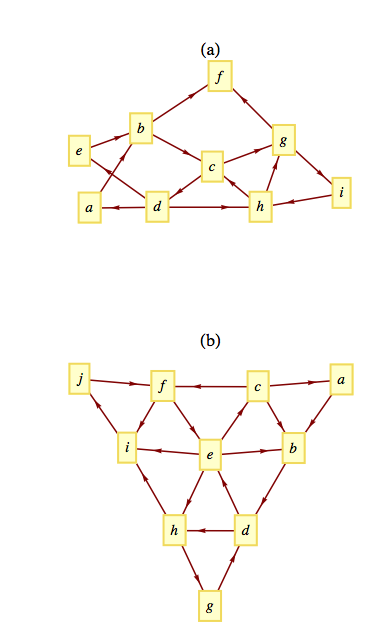
\includegraphics[width=0.6\linewidth]{images/fig-exercise-9-3-4.png}
\caption*{\textbf{Figure 9.3.12:} Shortest paths from \(a\) to \(i\)?}
\end{figure}
\end{divisionsolution}%
\begin{divisionsolution}{9.3.5.5}{}{exercise-374}%
\hypertarget{p-3222}{}%
Prove (by induction on \(k\)) that if the relation \(r\) on vertices of a graph is defined by \(v r w\) if there is an edge connecting \(v\) to \(w\), then \(r^k\), \(k \geq  1\), is defined by \(v r^kw\) if there is a path of length \(k\) from \(v\) to \(w\).%
\par\smallskip%
\noindent\textbf{Answer}.\quad%
\hypertarget{p-3223}{}%
Basis: \((k=1)\) Is the relation \(r^1\), defined by \(v r^1 w\) if there is a path of length 1 from \(v \text{ to } w\)? Yes, since \(v r w\) if and only if an edge, which is a path of length \(1\), connects \(v\) to \(w\).%
\par
\hypertarget{p-3224}{}%
Induction: Assume that \(v r^k w\) if and only if there is a path of length \(k\) from \(v\) to \(w\). We must show that \(v r^{k+1} w\) if and only if there is a path of length \(k+1\) from \(v\) to \(w\).%
\begin{equation*}
v r^{k+1} w \Rightarrow v r^k y \textrm{ and } y r w\textrm{ for some vertex } y
\end{equation*}
%
\par
\hypertarget{p-3225}{}%
By the induction hypothesis, there is a path of length \(k\) from \(v \textrm{ to } y\). And by the basis, there is a path of length one from \(y\) to \(w\). If we combine these two paths, we obtain a path of length \(k+1\) from \(v\) to \(w\). Of course, if we start with a path of length \(k+1\) from \(v\) to \(w\), we have a path of length \(k\) from \(v\) to some vertex \(y\) and a path of length 1 from \(y\) to \(w\). Therefore, \(v r^k y \textrm{ and } y r w \Rightarrow  v r^{k+1} w\).%
\end{divisionsolution}%
\section*{9.4 Traversals: Eulerian and Hamiltonian Graphs}
\addcontentsline{toc}{section}{9.4 Traversals: Eulerian and Hamiltonian Graphs}
\sectionmark{9.4 Traversals: Eulerian and Hamiltonian Graphs}
\subsection*{9.4.3 Exercises for Section 9.4}
\addcontentsline{toc}{subsection}{9.4.3 Exercises for Section 9.4}
\begin{divisionsolution}{9.4.3.1}{}{exercise-375}%
\hypertarget{p-3261}{}%
Locate a map of New York City and draw a graph that represents its land masses, bridges and tunnels. Is there an Eulerian path through New York? You can do the same with any other city that has at least two land masses.%
\par\smallskip%
\noindent\textbf{Answer}.\quad%
\hypertarget{p-3262}{}%
Using a recent road map, it appears that an Eulerian circuit exists in New York City, not including the small islands that belong to the city. Lowell, Massachusetts, is located at the confluence of the Merrimack and Concord rivers and has several canals flowing through it. No Eulerian path exists for Lowell.%
\end{divisionsolution}%
\begin{divisionsolution}{9.4.3.2}{}{exercise-376}%
\hypertarget{p-3263}{}%
Which of the drawings in Figure~9.4.23 can be drawn without removing your pencil from the paper and without drawing any line twice?%
\begin{figure}
\centering
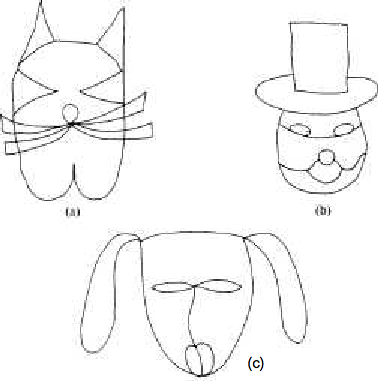
\includegraphics[width=0.65\linewidth]{images/fig-drawings-9-4.png}
\caption*{\textbf{Figure 9.4.23:} }
\end{figure}
\end{divisionsolution}%
\begin{divisionsolution}{9.4.3.3}{}{exercise-377}%
\hypertarget{p-3264}{}%
Write out the Gray Code for the 4-cube.%
\par\smallskip%
\noindent\textbf{Answer}.\quad%
\hypertarget{p-3265}{}%
Gray Code for the 4-cube:%
\begin{equation*}
G_4=\left(
\begin{array}{c}
0000 \\
0001 \\
0011 \\
0010 \\
0110 \\
0111 \\
0101 \\
0100 \\
1100 \\
1101 \\
1111 \\
1110 \\
1010 \\
1011 \\
1001 \\
1000 \\
\end{array}
\right)
\end{equation*}
%
\end{divisionsolution}%
\begin{divisionsolution}{9.4.3.4}{}{exercise-378}%
\hypertarget{p-3266}{}%
Find a Hamiltonian circuit for the dodecahedron graph in Figure~9.4.14.%
\end{divisionsolution}%
\begin{divisionsolution}{9.4.3.5}{}{exercise-379}%
\hypertarget{p-3267}{}%
The Euler Construction Company has been contracted to construct an extra bridge in Koenigsberg so that an Eulerian path through the town exists. Can this be done, and if so, where should the bridge be built?%
\par\smallskip%
\noindent\textbf{Answer}.\quad%
\hypertarget{p-3268}{}%
Any bridge between two land masses will be sufficient. To get an Eulerian circuit, you must add a second bridge that connects the two land masses that were not connected by the first bridge.%
\end{divisionsolution}%
\begin{divisionsolution}{9.4.3.6}{}{exercise-380}%
\hypertarget{p-3269}{}%
Consider the graphs in Figure~9.4.24. Determine which of the graphs have an Eulerian path, and find an Eulerian path for the graphs that have one.%
\begin{figure}
\centering
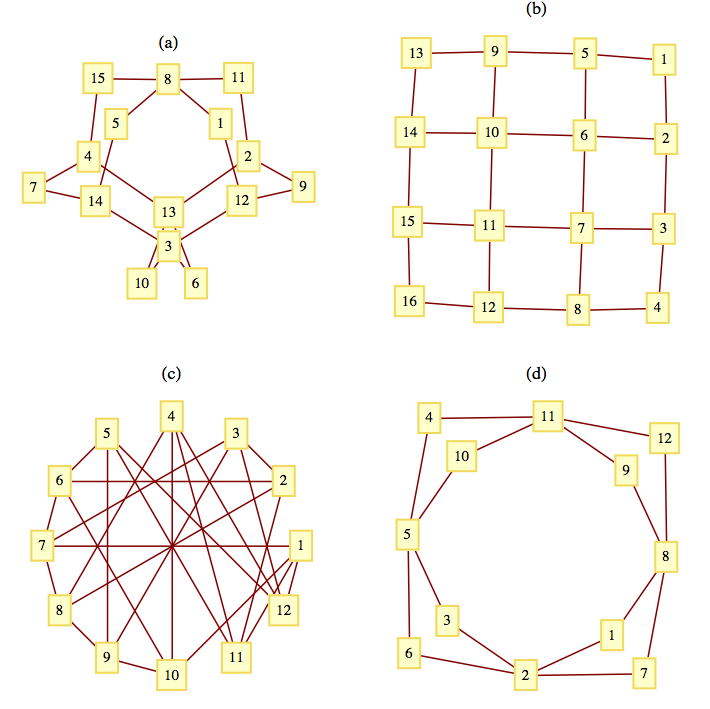
\includegraphics[width=1\linewidth]{images/fig-exercise-9-4-6.png}
\caption*{\textbf{Figure 9.4.24:} Graphs for exercise 6}
\end{figure}
\end{divisionsolution}%
\begin{divisionsolution}{9.4.3.7}{}{exercise-381}%
\hypertarget{p-3270}{}%
Formulate Euler's theorem for directed graphs.%
\par\smallskip%
\noindent\textbf{Answer}.\quad%
\hypertarget{p-3271}{}%
Let  \(G=(V,E)\) be a directed graph. \(G\) has an Eulerian circuit if and only if \(G\) is connected and \(indeg(v)= outdeg(v)\) for all \(v \in V\). There exists an Eulerian path from  \(v_1 \textrm{ to } v_2\)  if and only if \(G\) is connected, \(indeg(v_1)=outdeg(v_1)-1\), \(indeg(v_2)= outdeg(v_2)+1\), and for all other vertices in \(V\) the indegree and outdegree are equal.%
\end{divisionsolution}%
\begin{divisionsolution}{9.4.3.8}{}{exercise-382}%
\hypertarget{p-3272}{}%
Prove that the number of vertices in an undirected graph with odd degree must be even.%
\par\smallskip%
\noindent\textbf{Hint}.\quad%
\hypertarget{p-3273}{}%
Prove by induction on the number of edges.%
\end{divisionsolution}%
\begin{divisionsolution}{9.4.3.9}{}{exercise-383}%
\hypertarget{p-3274}{}%
\leavevmode%
\begin{enumerate}[label=(\alph*)]
\item\hypertarget{li-1547}{}\hypertarget{p-3275}{}%
Under what conditions will a round-robin tournament graph be Eulerian?%
\item\hypertarget{li-1548}{}\hypertarget{p-3276}{}%
Prove that every round-robin tournament graph is Hamiltonian.%
\end{enumerate}
%
\par\smallskip%
\noindent\textbf{Answer}.\quad%
\hypertarget{p-3277}{}%
A round-robin tournament graph is rarely Eulerian. It will be Eulerian if it has an odd number of vertices and each vertex (team) wins exactly as many times as it loses. Every round-robin tournament graph has a Hamiltonian path. This can be proven by induction on the number of vertices.%
\end{divisionsolution}%
\begin{divisionsolution}{9.4.3.10}{}{exercise-384}%
\hypertarget{p-3278}{}%
For what values of \(n\) is the \(n\)-cube Eulerian?%
\end{divisionsolution}%
\section*{9.5 Graph Optimization}
\addcontentsline{toc}{section}{9.5 Graph Optimization}
\sectionmark{9.5 Graph Optimization}
\subsection*{9.5.5 Exercises for Section 9.5}
\addcontentsline{toc}{subsection}{9.5.5 Exercises for Section 9.5}
\begin{divisionsolution}{9.5.5.1}{}{exercise-385}%
\hypertarget{p-3374}{}%
Find the closest neighbor circuit through the six capitals of New England starting at Boston. If you start at a different city, will you get a different circuit?%
\par\smallskip%
\noindent\textbf{Answer}.\quad%
\hypertarget{p-3375}{}%
The circuit would be Boston, Providence, Hartford, Concord, Montpelier, Augusta, Boston. It does matter where you start. If you start in Concord, for example, your mileage will be higher.%
\end{divisionsolution}%
\begin{divisionsolution}{9.5.5.2}{}{exercise-386}%
\hypertarget{p-3376}{}%
Is the estimate in Theorem~9.5.10 sharp for \(n = 3\)? For \(n = 4\)?%
\end{divisionsolution}%
\begin{divisionsolution}{9.5.5.3}{}{exercise-387}%
\hypertarget{p-3377}{}%
Given the following sets of points in the unit square, find the shortest circuit that visits all the points and find the circuit that is obtained with the strip algorithm.%
\par
\hypertarget{p-3378}{}%
\leavevmode%
\begin{enumerate}[label=(\alph*)]
\item\hypertarget{li-1583}{}\hypertarget{p-3379}{}%
\(\{(0.1k, 0.1k) : k = 0, 1, 2, . . . , 10\}\)%
\item\hypertarget{li-1584}{}\hypertarget{p-3380}{}%
\(\{(0.1, 0.3), (0.3, 0.8), (0.5, 0.3), (0.7, 0.9), (0.9, 0.1)\}\)%
\item\hypertarget{li-1585}{}\hypertarget{p-3381}{}%
\(\{(0.0, 0.5), (0.5, 0.0), (0.5, 1.0), (1.0, 0.5)\}\)%
\item\hypertarget{li-1586}{}\hypertarget{p-3382}{}%
\(\{(0, 0), (0.2, 0.6), (0.4, 0.1), (0.6, 0.8), (0.7, 0.5)\}\)%
\end{enumerate}
%
\par\smallskip%
\noindent\textbf{Answer}.\quad%
\hypertarget{p-3383}{}%
\leavevmode%
\begin{enumerate}[label=(\alph*)]
\item\hypertarget{li-1587}{}\hypertarget{p-3384}{}%
Optimal cost \(=2\sqrt{2}\). Phase 1 cost \(=2.4\sqrt{2}\). Phase 2 cost \(=2.6\sqrt{2}\).%
\item\hypertarget{li-1588}{}\hypertarget{p-3385}{}%
Optimal cost \(=2.60.\) Phase 1 cost \(=3.00\). Phase 2 cost \(2\sqrt{2}\).%
\item\hypertarget{li-1589}{}\hypertarget{p-3386}{}%
\(A=(0.0, 0.5), B=(0.5, 0.0), C=(0.5, 1.0), D=(1.0, 0.5)\)%
\par
\hypertarget{p-3387}{}%
There are 4 points; so we will divide the unit square into two strips.%
\begin{itemize}[label=\textbullet]
\item{}\hypertarget{p-3388}{}%
Optimal Path: \((B,A,C,D)\quad \quad \text{Distance } =2\sqrt{2}\)%
\item{}\hypertarget{p-3389}{}%
Phase I Path: \((B,A,C,D)\quad \quad \text{Distance }=2\sqrt{2}\)%
\item{}\hypertarget{p-3390}{}%
Phase II Path: \((A,C,B,D)\) \textbackslash{}quad \textbackslash{}quad\(\textrm{Distance }=2+\sqrt{2}\)%
\end{itemize}
%
\item\hypertarget{li-1593}{}\hypertarget{p-3391}{}%
\(A=(0,0), B=(0.2,0.6), C=(0.4,0.1), D=(0.6,0.8), E=(0.7,0.5)\)%
\par
\hypertarget{p-3392}{}%
There are 5 points; so we will divide the unit square into three strips.%
\begin{itemize}[label=\textbullet]
\item{}\hypertarget{p-3393}{}%
Optimal Path: \((A,B,D,E,C)\quad \quad \text{Distance }=2.31\)%
\item{}\hypertarget{p-3394}{}%
Phase I Path: \((A,C,B,C,E)\quad \quad \text{Distance }= 2.57\)%
\item{}\hypertarget{p-3395}{}%
Phase II Path: \((A,B,D,E,C) \quad \quad\textrm{Distance }=2.31\)%
\end{itemize}
%
\end{enumerate}
%
\end{divisionsolution}%
\begin{divisionsolution}{9.5.5.4}{}{exercise-388}%
\hypertarget{p-3396}{}%
For \(n = 4, 5, \text{and } 6\), locate \(n\) points in the unit square for which the strip algorithm works poorly.%
\end{divisionsolution}%
\begin{divisionsolution}{9.5.5.5}{}{exercise-389}%
\hypertarget{p-3397}{}%
Consider the network whose maximum capacities are shown on the following graph.%
\begin{figure}
\centering
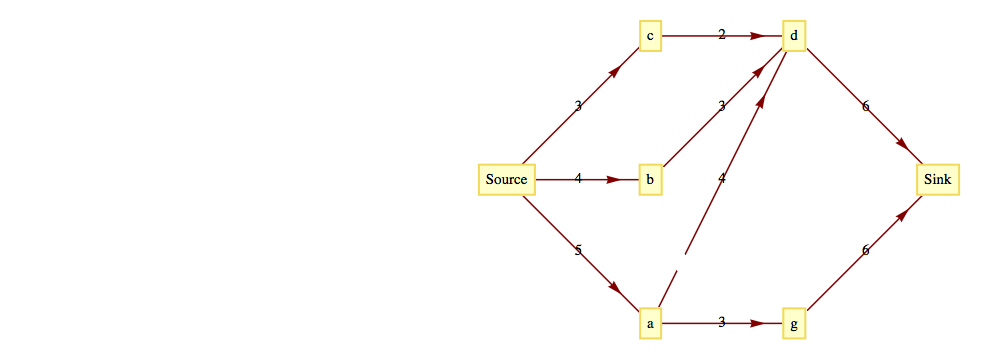
\includegraphics[width=1\linewidth]{images/fig-exercise-9-5-5.png}
\caption*{\textbf{Figure 9.5.30:} }
\end{figure}
\hypertarget{p-3398}{}%
\leavevmode%
\begin{enumerate}[label=(\alph*)]
\item\hypertarget{li-1597}{}\hypertarget{p-3399}{}%
A function \(f\) is partially defined on the edges of this network by: \(f(\text{Source}, c) =2\), \(f(\text{Source}, b) =2\), \(f(\text{Source}, a) = 2\), and \(f(a, d) = 1\).  Define \(f\) on the rest of the other edges so that \(f\) is a flow. What is the value of  \(f\) ?%
\item\hypertarget{li-1598}{}\hypertarget{p-3400}{}%
Find a flow augmenting path with respect to \(f\) for this network. What is the value of the augmented flow?%
\item\hypertarget{li-1599}{}\hypertarget{p-3401}{}%
Is the augmented flow a maximum flow? Explain.%
\end{enumerate}
%
\par\smallskip%
\noindent\textbf{Answer}.\quad%
\hypertarget{p-3402}{}%
\leavevmode%
\begin{enumerate}[label=(\alph*)]
\item\hypertarget{li-1600}{}\hypertarget{p-3403}{}%
\(f(c,d)=2\), \(f(b,d)=2\), \(f(d,k)=5\), \(f(a,g)=1\), and \(f(g,k)=1\).%
\item\hypertarget{li-1601}{}\hypertarget{p-3404}{}%
There are three possible flow-augmenting paths. \(s,b,d,k\) with flow increase of 1. \(s,a,d,k\) with flow increase of 1, and \(s,a,g,k\) with flow increase of 2.%
\item\hypertarget{li-1602}{}\hypertarget{p-3405}{}%
The new flow is never maximal, since another flow-augmenting path will always exist. For example, if \(s,b,d,k\) is used above, the new flow can be augmented by 2 units with \(s,a,g,k\).%
\end{enumerate}
%
\end{divisionsolution}%
\begin{divisionsolution}{9.5.5.6}{}{exercise-390}%
\hypertarget{p-3406}{}%
Given the following network with capacity function \(c\) and flow function \(f\), find a maximal flow function. The labels on thevedges of the network are of the form \(f(e)/c(e)\), where \(c(e)\) is the capacity of edge \(e\) and \(f(e)\) is the used capacity for flow \(f\).%
\begin{figure}
\centering
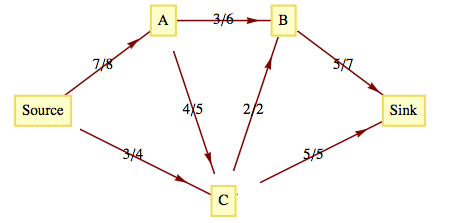
\includegraphics[width=0.7\linewidth]{images/fig-exercise-9-5-6.png}
\caption*{\textbf{Figure 9.5.31:} }
\end{figure}
\end{divisionsolution}%
\begin{divisionsolution}{9.5.5.7}{}{exercise-391}%
\hypertarget{p-3407}{}%
Find maximal flows for the following networks.%
\begin{sidebyside}{2}{0}{0}{0}%
\begin{sbspanel}{0.5}%
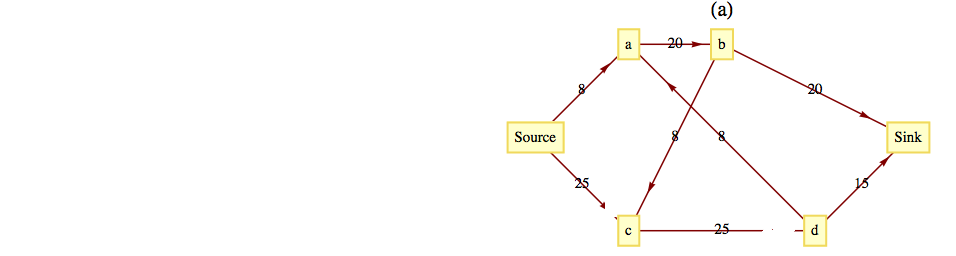
\includegraphics[width=1\linewidth]{images/fig-exercise-9-5-7a.png}
\end{sbspanel}%
\begin{sbspanel}{0.5}%
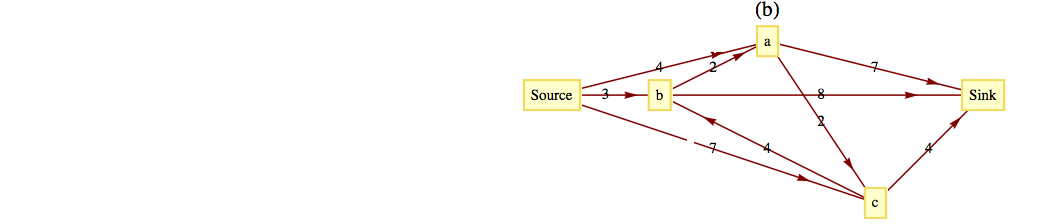
\includegraphics[width=1\linewidth]{images/fig-exercise-9-5-7b.png}
\end{sbspanel}%
\nopagebreak%
\begin{sbscaption}{0.5}%
\captionof*{figure}{\textbf{Figure 9.5.32:} }
\end{sbscaption}%
\begin{sbscaption}{0.5}%
\captionof*{figure}{\textbf{Figure 9.5.33:} }
\end{sbscaption}%
\end{sidebyside}%
\begin{figure}
\centering
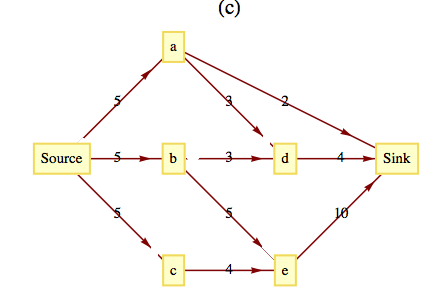
\includegraphics[width=0.7\linewidth]{images/fig-exercise-9-5-7c.png}
\caption*{\textbf{Figure 9.5.34:} }
\end{figure}
\par\smallskip%
\noindent\textbf{Answer}.\quad%
\hypertarget{p-3408}{}%
\leavevmode%
\begin{enumerate}[label=(\alph*)]
\item\hypertarget{li-1603}{}\hypertarget{p-3409}{}%
Value of maximal flow \(=31\).%
\item\hypertarget{li-1604}{}\hypertarget{p-3410}{}%
Value of maximal flow \(=14\).%
\item\hypertarget{li-1605}{}\hypertarget{p-3411}{}%
Value of maximal flow \(=14\). See Table~9.5.35 for one way to got this flow.%
\end{enumerate}
%
\begin{table}
\centering
\begin{tabular}{ccc}\hrulethick
Step&Flow-augmenting path&Flow added\tabularnewline[0pt]
1&\(\text{Source},A,\text{Sink}\)&2\tabularnewline[0pt]
2&\(\text{Source}, C,B, \text{Sink}\)&3\tabularnewline[0pt]
3&\(\text{Source},E,D, \text{Sink}\)&4\tabularnewline[0pt]
4&\(\text{Source},A,B,\text{Sink}\)&1\tabularnewline[0pt]
5&\(\text{Source},C,D, \text{Sink}\)&2\tabularnewline[0pt]
6&\(\text{Source},A,B,C,D, \text{Sink}\)&2
\end{tabular}
\caption*{\textbf{Table 9.5.35:} }
\end{table}
\end{divisionsolution}%
\begin{divisionsolution}{9.5.5.8}{}{exercise-392}%
\hypertarget{p-3412}{}%
\leavevmode%
\begin{enumerate}[label=(\alph*)]
\item\hypertarget{li-1606}{}\hypertarget{p-3413}{}%
Find two maximal flows for the network in Figure~9.5.28 other than the one found in the text.%
\item\hypertarget{li-1607}{}\hypertarget{p-3414}{}%
Describe the set of all maximal flows for the same network.%
\item\hypertarget{li-1608}{}\hypertarget{p-3415}{}%
Prove that if a network has two maximal flows, then it has an infinite number of maximal flows.%
\end{enumerate}
%
\end{divisionsolution}%
\begin{divisionsolution}{9.5.5.9}{}{exercise-393}%
\hypertarget{p-3416}{}%
Discuss reasons that the closest neighbor algorithm is not used in the unit square version of the Traveling Salesman Problem.%
\par\smallskip%
\noindent\textbf{Hint}.\quad%
\hypertarget{p-3417}{}%
Count the number of comparisons of distances that must be done.%
\par\smallskip%
\noindent\textbf{Answer}.\quad%
\hypertarget{p-3418}{}%
To locate the closest neighbor among the list of \(k\) other points on the unit square requires a time proportional to \(k\). Therefore the time required for the closest-neighbor algorithm with \(n\) points is proportional to \((n-1)+(n-2)+\cdots +2+1\), which is proportional to \(n^2\). Since the strip algorithm takes a time proportional to \(n(\log  n)\), it is much faster for large values of \(n\).%
\end{divisionsolution}%
\begin{divisionsolution}{9.5.5.10}{}{exercise-394}%
\hypertarget{p-3419}{}%
Explore the possibility of solving the Traveling Salesman Problem in the ``unit box'': \([0,1]^3\).%
\end{divisionsolution}%
\begin{divisionsolution}{9.5.5.11}{}{exercise-395}%
\hypertarget{p-3420}{}%
Devise a ``closest neighbor'' algorithm for matching points in the unit square.%
\end{divisionsolution}%
\section*{9.6 Planarity and Colorings}
\addcontentsline{toc}{section}{9.6 Planarity and Colorings}
\sectionmark{9.6 Planarity and Colorings}
\subsection*{9.6.1 Planar Graphs}
\addcontentsline{toc}{subsection}{9.6.1 Planar Graphs}
\begin{activitysolution}{9.6.1}{}{activity-1}%
\leavevmode%
\begin{enumerate}[font=\bfseries,label=(\alph*),ref=\alph*]
\item[(a)] \hypertarget{p-3434}{}%
Experiment: Jot down a graph right now and count the number of vertices, regions, and edges that you have. If \(v + r - e\) is not 2, then your graph is either nonplanar or not connected.%
\end{enumerate}
\end{activitysolution}%
\subsection*{9.6.3 Exercises for Section 9.6}
\addcontentsline{toc}{subsection}{9.6.3 Exercises for Section 9.6}
\begin{divisionsolution}{9.6.3.1}{}{exercise-396}%
\hypertarget{p-3478}{}%
Apply Theorem~9.6.12 to prove that once \(n\) gets to a certain size, a \(K_n\) is nonplanar. What is the largest complete planar graph?%
\par\smallskip%
\noindent\textbf{Answer}.\quad%
\hypertarget{p-3479}{}%
Theorem~9.6.12 can be applied to infer that if \(n\geqslant 5\), then \(K_n\) is nonplanar. A \(K_4\) is the largest complete planar graph.%
\end{divisionsolution}%
\begin{divisionsolution}{9.6.3.2}{}{exercise-397}%
\hypertarget{p-3480}{}%
Can you apply Theorem~9.6.12 to prove that the Three Utilities Puzzle can't be solved?%
\end{divisionsolution}%
\begin{divisionsolution}{9.6.3.3}{}{exercise-398}%
\hypertarget{p-3481}{}%
What are the chromatic numbers of the following graphs?%
\begin{figure}
\centering
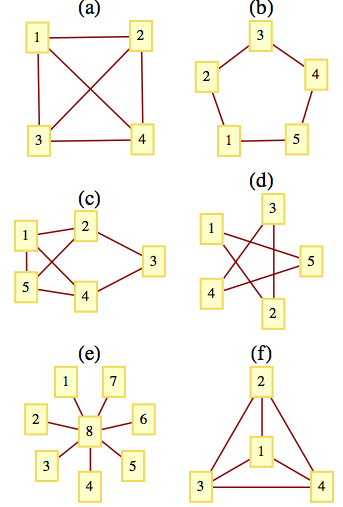
\includegraphics[width=0.7\linewidth]{images/fig-exercise-9-6-3.png}
\caption*{\textbf{Figure 9.6.21:} What are the chromatic numbers?}
\end{figure}
\par\smallskip%
\noindent\textbf{Answer}.\quad%
\hypertarget{p-3482}{}%
\leavevmode%
\begin{multicols}{3}
\begin{enumerate}[label=(\alph*)]
\item\hypertarget{li-1621}{}\hypertarget{p-3483}{}%
4%
\item\hypertarget{li-1622}{}\hypertarget{p-3484}{}%
3%
\item\hypertarget{li-1623}{}\hypertarget{p-3485}{}%
3%
\item\hypertarget{li-1624}{}\hypertarget{p-3486}{}%
3%
\item\hypertarget{li-1625}{}\hypertarget{p-3487}{}%
2%
\item\hypertarget{li-1626}{}\hypertarget{p-3488}{}%
4%
\end{enumerate}
\end{multicols}
%
\end{divisionsolution}%
\begin{divisionsolution}{9.6.3.4}{}{exercise-399}%
\hypertarget{p-3489}{}%
Prove that if an undirected graph has a subgraph that is a \(K_3\) it then its chromatic number is at least 3.%
\end{divisionsolution}%
\begin{divisionsolution}{9.6.3.5}{}{exercise-400}%
\hypertarget{p-3490}{}%
What is \(\chi \left(K_n\right)\), \(n\geq 1\)?%
\par\smallskip%
\noindent\textbf{Answer}.\quad%
\hypertarget{p-3491}{}%
The chromatic number is \(n\) since every vertex is connected to every other vertex.%
\end{divisionsolution}%
\begin{divisionsolution}{9.6.3.6}{}{exercise-401}%
\hypertarget{p-3492}{}%
What is the chromatic number of the United States?%
\end{divisionsolution}%
\begin{divisionsolution}{9.6.3.7}{}{exercise-402}%
\hypertarget{p-3493}{}%
Complete the proof of Euler's Formula.%
\par\smallskip%
\noindent\textbf{Answer}.\quad%
\hypertarget{p-3494}{}%
Suppose that \(G'\) is not connected. Then \(G'\) is made up of 2 components that are planar graphs with less than \(k\) edges, \(G_1\) and \(G_2\). For \(i=1,2\) let \(v_i,r_i, \text{and} e_i\) be the number of vertices, regions and edges in \(G_i\). By the induction hypothesis, \(v_i+r_i-e_i=2\) for \(i=1,2\).%
\par
\hypertarget{p-3495}{}%
One of the regions, the infinite one, is common to both graphs. Therefore, when we add edge \(e\) back to the graph, we have \(r=r_1+r_2-1\), \(v=v_1+v_2\), and  \(e=e_1+e_2+1\).%
\begin{equation*}
\begin{split}
v+r-e &=\left(v_1+v_2\right)+\left(r_1+r_2-1\right)-\left(e_1+e_2+1\right)\\
&=\left(v_1+r_1-e_1\right)+\left(v_2+r_2-e_2\right)-2\\
&=2 + 2 -2\\
&=2
\end{split}
\end{equation*}
%
\end{divisionsolution}%
\begin{divisionsolution}{9.6.3.8}{}{exercise-403}%
\hypertarget{p-3496}{}%
Use the outline of a proof of Theorem~9.6.10 to write a complete proof. Be sure to point out where the premise \(v\geq 3\) is essential.%
\end{divisionsolution}%
\begin{divisionsolution}{9.6.3.9}{}{exercise-404}%
\hypertarget{p-3497}{}%
Let \(G = (V,E)\) with \(|V|\geq 11\), and let \(U\) be the set of all undirected edges between distinct vertices in \(V\).  Prove that either \(G\) or \(G' = \left(V,E^c\right)\) is nonplanar.%
\par\smallskip%
\noindent\textbf{Answer}.\quad%
\hypertarget{p-3498}{}%
Since \(\left| E\right| +E^c=\frac{n(n-1)}{2}\), either \(E \text{ or } E^c\) has at least \(\frac{n(n-1)}{4}\) elements. Assume that it is \(E\) that is larger. Since \(\frac{n(n-1)}{4}\) is greater than \(3n-6\text{  }\text{for}\text{  }n\geqslant 11\), \(G\) would be nonplanar. Of course, if \(E^c\) is larger, then \(G'\) would be nonplanar by the same reasoning.  Can you find a graph with ten vertices such that it is planar and its complement is also planar?%
\end{divisionsolution}%
\begin{divisionsolution}{9.6.3.10}{}{exercise-405}%
\hypertarget{p-3499}{}%
Design an algorithm to determine whether a graph is bipartite.%
\end{divisionsolution}%
\begin{divisionsolution}{9.6.3.11}{}{exercise-406}%
\hypertarget{p-3500}{}%
Prove that a bipartite graph with an odd number of vertices greater than or equal to 3 has no Hamiltonian circuit.%
\par\smallskip%
\noindent\textbf{Answer}.\quad%
\hypertarget{p-3501}{}%
Suppose that \((V,E)\) is bipartite (with colors red and blue), \(\left| E\right|\) is odd, and \(\left(v_1,v_2,\ldots ,v_{2n+1},v_1\right)\) is a Hamiltonian circuit. If \(v_1\) is red, then \(v_{2n+1}\) would also be red. But then \(\left\{v_{2n+1},v_1\right\}\) would not be in \(E\), a contradiction.%
\end{divisionsolution}%
\begin{divisionsolution}{9.6.3.12}{}{exercise-407}%
\hypertarget{p-3502}{}%
Prove that any graph with a finite number of vertices can be drawn in three dimensions so that no edges intersect.%
\end{divisionsolution}%
\begin{divisionsolution}{9.6.3.13}{}{exercise-408}%
\hypertarget{p-3503}{}%
Suppose you had to color the edges of an undirected graph so that for each vertex, the edges that it is connected to have different colors. How can this problem be transformed into a vertex coloring problem?%
\par\smallskip%
\noindent\textbf{Answer}.\quad%
\hypertarget{p-3504}{}%
Draw a graph with one vertex for each edge, If two edges in the original graph meet at the same vertex, then draw an edge connecting the corresponding  vertices in the new graph.%
\end{divisionsolution}%
\begin{divisionsolution}{9.6.3.14}{}{exercise-409}%
\hypertarget{p-3505}{}%
\leavevmode%
\begin{enumerate}[label=(\alph*)]
\item\hypertarget{li-1627}{}\hypertarget{p-3506}{}%
Suppose the edges of a \(K_6\) are colored either red or blue. Prove that there will be either a ``red \(K_3\)'' (a subset of the vertex set with three vertices connected by red edges) or a ``blue \(K_3\)'' or both.%
\item\hypertarget{li-1628}{}\hypertarget{p-3507}{}%
Suppose six people are selected at random. Prove that either there exists a subset of three of them with the property that any two people in the subset can communicate in a common language, or there exist three people, no two of whom can communicate in a common language.%
\end{enumerate}
%
\end{divisionsolution}%
\begin{divisionsolution}{9.6.3.15}{}{exercise-410}%
\hypertarget{p-3508}{}%
\index{Mesh Graph}Let \(d\) be a positive integer, and let \(a_1, a_2, \dots a_d\) be positive integers greater than or equal to two.  The \terminology{mesh graph} \(M(a_1,a_2,\dots,a_d)\) has vertices of the form \(x=(x_1, x_2,\dots, x_d)\) where \(1 \leq x_i \leq a_i\). Two vertices \(x\) and \(y\) are adjacent if and only if \(\sum_{i=1}^{d}{\lvert x_i-y_i \rvert} = 1\).  In other words, two adjacent vertices must differ in only one coordinate and by a difference of 1.%
\par
\hypertarget{p-3509}{}%
\leavevmode%
\begin{enumerate}[label=(\alph*)]
\item\hypertarget{li-1629}{}\hypertarget{p-3510}{}%
What is the chromatic number of  \(M(a_1,a_2,\dots,a_d)\)?%
\item\hypertarget{li-1630}{}\hypertarget{p-3511}{}%
For what pairs  \((a_1, a_2)\) does \(M(a_1, a_2)\) have a Hamiltonian circuit?%
\item\hypertarget{li-1631}{}\hypertarget{p-3512}{}%
For what triples   \((a_1, a_2, a_3)\) does \(M(a_1, a_2, a_3)\) have a Hamiltonian circuit?%
\end{enumerate}
%
\end{divisionsolution}%
\chapter*{10 Trees}
\addcontentsline{toc}{chapter}{10 Trees}
\chaptermark{10 Trees}
\section*{10.1 What Is a Tree?}
\addcontentsline{toc}{section}{10.1 What Is a Tree?}
\sectionmark{10.1 What Is a Tree?}
\subsection*{10.1.3 Exercises for Section 10.1}
\addcontentsline{toc}{subsection}{10.1.3 Exercises for Section 10.1}
\begin{divisionsolution}{10.1.3.1}{}{exercise-trees}%
\hypertarget{p-3543}{}%
Given the following vertex sets, draw all possible undirected trees that connect them.%
\par
\hypertarget{p-3544}{}%
\leavevmode%
\begin{enumerate}[label=(\alph*)]
\item\hypertarget{li-1641}{}\hypertarget{p-3545}{}%
\(V_a= \{\text{right},\text{left}\}\)%
\item\hypertarget{li-1642}{}\hypertarget{p-3546}{}%
\(V_b = \{+,-,0\}\)%
\item\hypertarget{li-1643}{}\hypertarget{p-3547}{}%
\(V_c = \{\text{north}, \text{south}, \text{east}, \text{west}\}\).%
\end{enumerate}
%
\par\smallskip%
\noindent\textbf{Answer}.\quad%
\hypertarget{p-3548}{}%
The number of trees are: (a) 1, (b) 3, and (c) 16.  The trees that connect \(V_c\) are:%
\begin{figure}
\centering
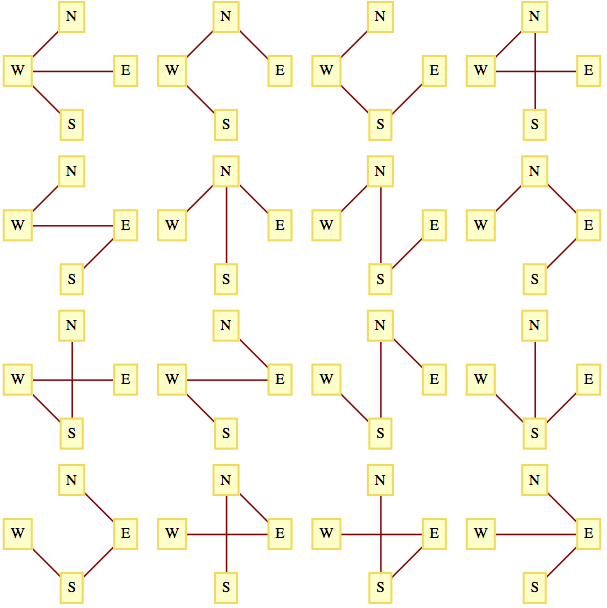
\includegraphics[width=1\linewidth]{images/fig-sol-10-1-1.png}
\caption*{\textbf{Figure 10.1.12:} }
\end{figure}
\end{divisionsolution}%
\begin{divisionsolution}{10.1.3.2}{}{exercise-412}%
\hypertarget{p-3549}{}%
Are all trees planar? If they are, can you explain why? If they are not, you should be able to find a nonplanar tree.%
\end{divisionsolution}%
\begin{divisionsolution}{10.1.3.3}{}{exercise-413}%
\hypertarget{p-3550}{}%
Prove that if \(G\) is a simple undirected graph with no self-loops, then \(G\) is a tree if and only if \(G\) is connected and \(\lvert E \rvert = \lvert V \rvert - 1\).%
\par\smallskip%
\noindent\textbf{Hint}.\quad%
\hypertarget{p-3551}{}%
Use induction on \(\lvert E\rvert \).%
\end{divisionsolution}%
\begin{divisionsolution}{10.1.3.4}{}{exercise-414}%
\hypertarget{p-3552}{}%
\leavevmode%
\begin{enumerate}[label=(\alph*)]
\item\hypertarget{li-1644}{}\hypertarget{p-3553}{}%
Prove that if \(G = (V, E)\) is a tree and \(e \in E\), then \((V, E - \{e\})\) is a forest of two trees.%
\item\hypertarget{li-1645}{}\hypertarget{p-3554}{}%
Prove that if \(\left(V_1,E_1\right.\)) and \(\left(V_2,E_2\right)\) are disjoint trees and \(e\) is an edge that connects a vertex in \(V_1\) to a vertex in \(V_2\), then \(\left(V_1\cup V_2, E_1\cup E_2\cup \{e\}\right)\) is a tree.%
\end{enumerate}
%
\end{divisionsolution}%
\begin{divisionsolution}{10.1.3.5}{}{exercise-415}%
\hypertarget{p-3555}{}%
\leavevmode%
\begin{enumerate}[label=(\alph*)]
\item\hypertarget{li-1646}{}\hypertarget{p-3556}{}%
Prove that any tree with at least two vertices has at least two vertices of degree 1.%
\item\hypertarget{li-1647}{}\hypertarget{p-3557}{}%
Prove that if a tree has \(n\) vertices,  \(n \geq 4\), and is not a path graph, \(P_n\), then it has at least three vertices of degree 1.%
\end{enumerate}
%
\par\smallskip%
\noindent\textbf{Answer}.\quad%
\hypertarget{p-3558}{}%
\leavevmode%
\begin{enumerate}[label=(\alph*)]
\item\hypertarget{li-1648}{}\hypertarget{p-3559}{}%
Assume that \((V,E)\) is a tree with \(\left| V\right| \geq 2\), and all but possibly one vertex in \(V\) has degree two or more.%
\begin{equation*}
\begin{split}
2\lvert E \rvert =\sum_{v \in V}{\deg(v)} \geq 2 \lvert V \rvert -1 &\Rightarrow
\lvert E\vert  \geq \lvert V\rvert -\frac{1}{2}\\
&\Rightarrow \lvert E\rvert \geq \lvert V\rvert\\
& \Rightarrow (V,E) \textrm{ is not a tree.}
\end{split}
\end{equation*}
%
\item\hypertarget{li-1649}{}\hypertarget{p-3560}{}%
The proof of this part is similar to part a in that we can infer \(2\lvert E\rvert \geq 2 \lvert V\rvert -1\), using the fact that a non-chain tree has at least one vertex of degree three or more.%
\end{enumerate}
%
\end{divisionsolution}%
\section*{10.2 Spanning Trees}
\addcontentsline{toc}{section}{10.2 Spanning Trees}
\sectionmark{10.2 Spanning Trees}
\subsection*{10.2.4 Exercises for Section 10.2}
\addcontentsline{toc}{subsection}{10.2.4 Exercises for Section 10.2}
\begin{divisionsolution}{10.2.4.1}{}{exercise-416}%
\hypertarget{p-3597}{}%
Suppose that after Atlantis University's phone system is in place, a fifth campus is established and that a transmission line can be bought to connect the new campus to any old campus. Is this larger system the most economical one possible with respect to Objective 1? Can you always satisfy Objective 2?%
\par\smallskip%
\noindent\textbf{Answer}.\quad%
\hypertarget{p-3598}{}%
It might not be most economical with respect to Objective 1. You should be able to find an example to illustrate this claim. The new system can always be made most economical with respect to Objective 2 if the old system were designed with that objective in mind.%
\end{divisionsolution}%
\begin{divisionsolution}{10.2.4.2}{}{exercise-417}%
\hypertarget{p-3599}{}%
Construct a minimal spanning tree for the capital cities in New England (see Table~9.5.3).%
\end{divisionsolution}%
\begin{divisionsolution}{10.2.4.3}{}{exercise-418}%
\hypertarget{p-3600}{}%
Show that the answer to the question posed in Example~10.2.7 is ``no.''%
\par\smallskip%
\noindent\textbf{Answer}.\quad%
\hypertarget{p-3601}{}%
In the figure below, \(\{1,2\}\) is not a minimal bridge between \(L=\{1,4\} \textrm{ and } R=\{2,3\}\), but it is part of the minimal spanning tree for this graph.%
\begin{figure}
\centering
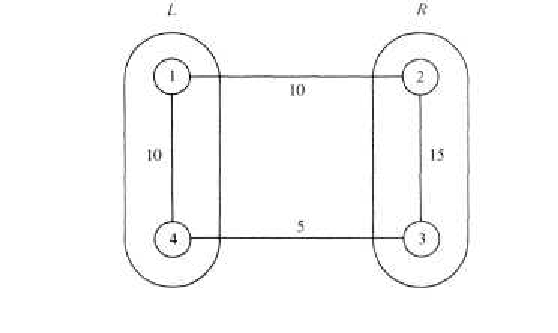
\includegraphics[width=0.8\linewidth]{images/fig-sol-e-10-2-3.png}
\caption*{\textbf{Figure 10.2.16:} }
\end{figure}
\end{divisionsolution}%
\begin{divisionsolution}{10.2.4.4}{}{exercise-419}%
\hypertarget{p-3602}{}%
Find a minimal spanning tree for the following graphs.%
\begin{figure}
\centering
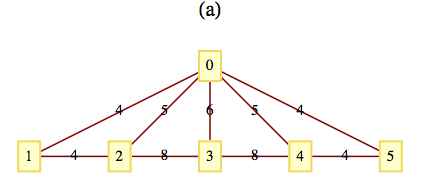
\includegraphics[width=0.8\linewidth]{images/fig-exercise-10-2-4a.png}
\caption*{\textbf{Figure 10.2.17:} }
\end{figure}
\begin{figure}
\centering
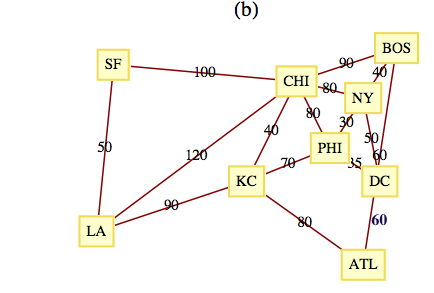
\includegraphics[width=0.8\linewidth]{images/fig-exercise-10-2-4b.png}
\caption*{\textbf{Figure 10.2.18:} }
\end{figure}
\begin{figure}
\centering
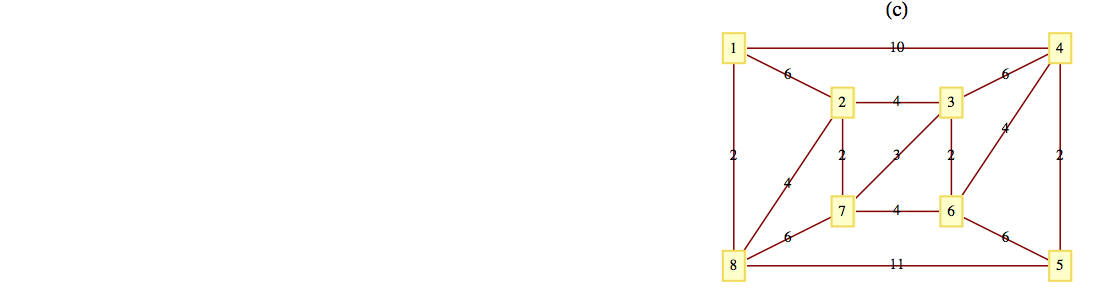
\includegraphics[width=0.7\linewidth]{images/fig-exercise-10-2-4c.png}
\caption*{\textbf{Figure 10.2.19:} }
\end{figure}
\end{divisionsolution}%
\begin{divisionsolution}{10.2.4.5}{}{exercise-420}%
\hypertarget{p-3603}{}%
Find a minimum diameter spanning tree for the following graphs.%
\begin{figure}
\centering
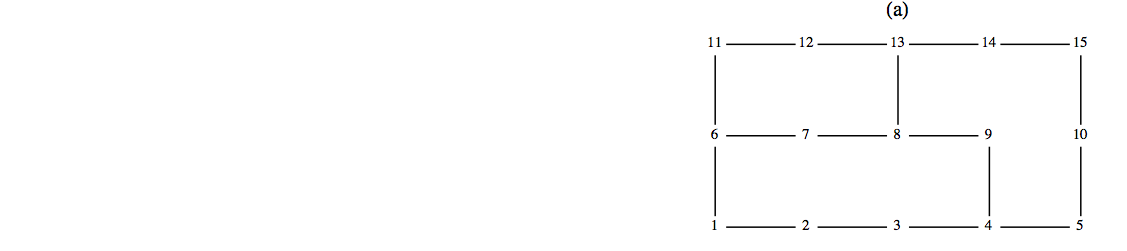
\includegraphics[width=0.8\linewidth]{images/fig-exercise-10-2-5a.png}
\caption*{\textbf{Figure 10.2.20:} }
\end{figure}
\begin{figure}
\centering
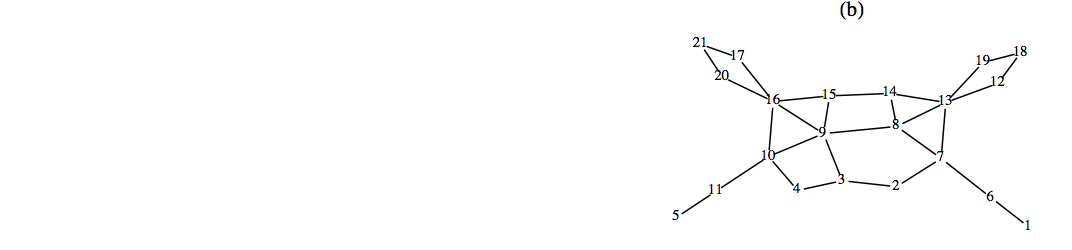
\includegraphics[width=0.8\linewidth]{images/fig-exercise-10-2-5b.png}
\caption*{\textbf{Figure 10.2.21:} }
\end{figure}
\par\smallskip%
\noindent\textbf{Answer}.\quad%
\hypertarget{p-3604}{}%
\leavevmode%
\begin{enumerate}[label=(\alph*)]
\item\hypertarget{li-1663}{}\hypertarget{p-3605}{}%
Edges in one solution are: \(\{8,7\},\{8,9\},\{8,13\},\{7,6\},\{9,4\},\{13,12\},\{13,14\},\{6,11\},\{6,1\},\{1,2\},\{4,3\},\{4,5\},\{14,15\},
\textrm{ and } \{5,10\}\)%
\item\hypertarget{li-1664}{}\hypertarget{p-3606}{}%
Vertices 8 and 9 are centers of the graph. Starting from vertex 8, a minimum diameter spanning tree is \(\{\{8, 3\}, \{8, 7\}, \{8, 13\},
\{8, 14\}, \{8, 9\}, \{3, 2\}, \{3, 4\}, \{7, 6\}, \{13, 12\}, \{13, 19\}, \{14, 15\}, \{9, 16\}, \{9, 10\}, \{6, 1\}, \{12, 18\}, \{16, 20\}, \{16,
17\}, \{10, 11\}, \{20, 21\}, \{11, 5\}\}.\)    The diameter of the tree is 7.%
\end{enumerate}
%
\end{divisionsolution}%
\begin{divisionsolution}{10.2.4.6}{}{exercise-421}%
\hypertarget{p-3607}{}%
In each of the following parts justify your answer with either a proof or a counterexample.%
\par
\hypertarget{p-3608}{}%
\leavevmode%
\begin{enumerate}[label=(\alph*)]
\item\hypertarget{li-1665}{}\hypertarget{p-3609}{}%
Suppose a weighted undirected graph had distinct edge weights. Is it possible that no minimal spanning tree includes the edge of minimal weight?%
\item\hypertarget{li-1666}{}\hypertarget{p-3610}{}%
Suppose a weighted undirected graph had distinct edge weights. Is it possible that every minimal spanning tree includes the edge of maximal weight? If true, under what conditions would it happen?%
\end{enumerate}
%
\end{divisionsolution}%
\section*{10.3 Rooted Trees}
\addcontentsline{toc}{section}{10.3 Rooted Trees}
\sectionmark{10.3 Rooted Trees}
\subsection*{10.3.4 Exercises for Section 10.3}
\addcontentsline{toc}{subsection}{10.3.4 Exercises for Section 10.3}
\begin{divisionsolution}{10.3.4.1}{}{exercise-422}%
\hypertarget{p-3646}{}%
Suppose that an undirected tree has diameter \(d\) and that you would like to select a vertex of the tree as a root so that the resulting rooted tree has the smallest depth possible. How would such a root be selected and what would be the depth of the tree (in terms of \(d\))?%
\par\smallskip%
\noindent\textbf{Answer}.\quad%
\hypertarget{p-3647}{}%
Locate any simple path of length \(d\) and locate the vertex in position \(\lceil d/2\rceil\) on the path. The tree rooted at that vertex will have a depth of \(\lceil d/2\rceil\), which is minimal.%
\end{divisionsolution}%
\begin{divisionsolution}{10.3.4.2}{}{exercise-423}%
\hypertarget{p-3648}{}%
Use Kruskal's algorithm to find a minimal spanning tree for the following graphs. In addition to the spanning tree, find the final rooted tree in the algorithm.  When you merge two trees in the algorithm, make the root with the lower number the root of the new tree.%
\begin{figure}
\centering
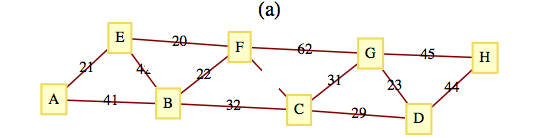
\includegraphics[width=1\linewidth]{images/fig-exercise-10-3-2a.png}
\caption*{\textbf{Figure 10.3.13:} }
\end{figure}
\begin{figure}
\centering
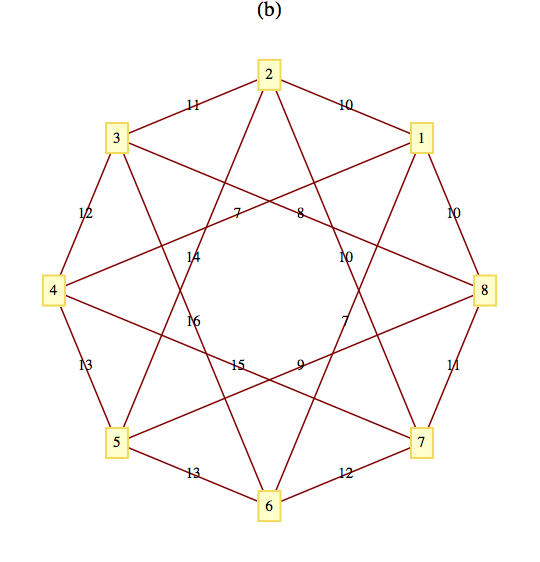
\includegraphics[width=1\linewidth]{images/fig-exercise-10-3-2b.png}
\caption*{\textbf{Figure 10.3.14:} }
\end{figure}
\end{divisionsolution}%
\begin{divisionsolution}{10.3.4.3}{}{exercise-424}%
\hypertarget{p-3649}{}%
Suppose that information on buildings is arranged in records with five fields: the name of the building, its location, its owner, its height, and its floor space. The location and owner fields are records that include all of the information that you would expect, such as street, city, and state, together with the owner's name (first, middle, last) in the owner field. Draw a rooted tree to describe this type of record%
\par\smallskip%
\noindent\textbf{Answer}.\quad%
\leavevmode%
\begin{figure}
\centering
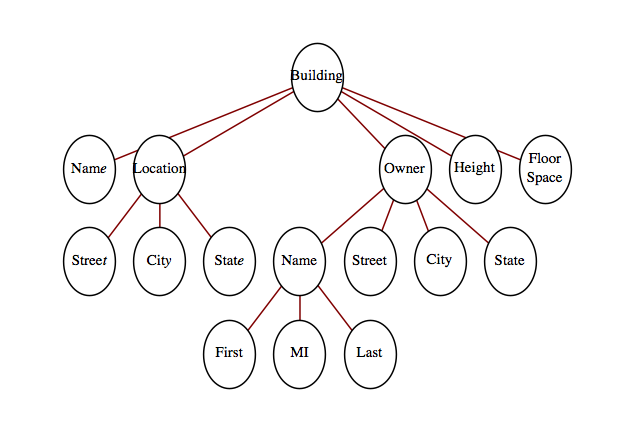
\includegraphics[width=1\linewidth]{images/fig-solution-10-3-3.png}
\caption*{\textbf{Figure 10.3.15:} }
\end{figure}
\end{divisionsolution}%
\begin{divisionsolution}{10.3.4.4}{}{exercise-425}%
\hypertarget{p-3650}{}%
Step through Kruskel's Algorthm by hand to verify that the example of a minimal spanning tree using Sage in Subsection~10.3.3 is correct.%
\end{divisionsolution}%
\section*{10.4 Binary Trees}
\addcontentsline{toc}{section}{10.4 Binary Trees}
\sectionmark{10.4 Binary Trees}
\subsection*{10.4.6 Exercises for Section 10.4}
\addcontentsline{toc}{subsection}{10.4.6 Exercises for Section 10.4}
\begin{divisionsolution}{10.4.6.1}{}{exercise-426}%
\hypertarget{p-3736}{}%
Draw the expression trees for the following expressions:%
\par
\hypertarget{p-3737}{}%
\leavevmode%
\begin{enumerate}[label=(\alph*)]
\item\hypertarget{li-1719}{}\hypertarget{p-3738}{}%
\(a(b + c)\)%
\item\hypertarget{li-1720}{}\hypertarget{p-3739}{}%
\(a b + c\)%
\item\hypertarget{li-1721}{}\hypertarget{p-3740}{}%
\(a b + a c\)%
\item\hypertarget{li-1722}{}\hypertarget{p-3741}{}%
\(b b - 4 a c\)%
\item\hypertarget{li-1723}{}\hypertarget{p-3742}{}%
\(\left(\left(a_3 x + a_2\right)x +a_1\right)x + a_0\)%
\end{enumerate}
%
\par\smallskip%
\noindent\textbf{Answer}.\quad%
\leavevmode%
\begin{figure}
\centering
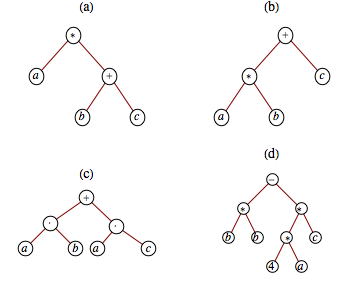
\includegraphics[width=0.8\linewidth]{images/fig-sol-10-4-1-A.png}
\caption*{\textbf{Figure 10.4.15:} }
\end{figure}
\begin{figure}
\centering
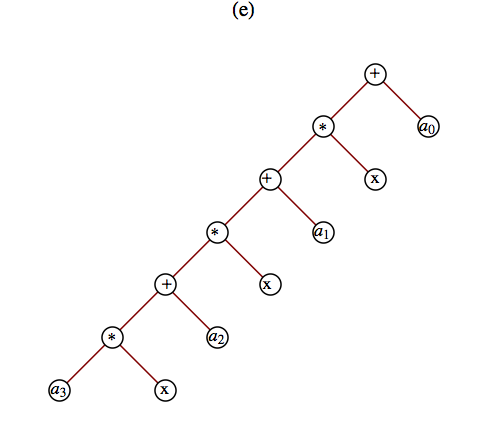
\includegraphics[width=0.7\linewidth]{images/fig-sol-10-4-1-B.png}
\caption*{\textbf{Figure 10.4.16:} }
\end{figure}
\end{divisionsolution}%
\begin{divisionsolution}{10.4.6.2}{}{exercise-427}%
\hypertarget{p-3743}{}%
Draw the expression trees for%
\par
\hypertarget{p-3744}{}%
\leavevmode%
\begin{enumerate}[label=(\alph*)]
\item\hypertarget{li-1724}{}\hypertarget{p-3745}{}%
\(\frac{x^2-1}{x-1}\)%
\item\hypertarget{li-1725}{}\hypertarget{p-3746}{}%
\(x y + x z + y z\)%
\end{enumerate}
%
\end{divisionsolution}%
\begin{divisionsolution}{10.4.6.3}{}{exercise-428}%
\hypertarget{p-3747}{}%
Write out the preorder, inorder, and postorder traversals of the trees in Exercise 1 above.%
\par\smallskip%
\noindent\textbf{Answer}.\quad%
\hypertarget{p-3748}{}%
%
\begin{equation*}
\begin{array}{cccc}
& \text{Preorder}  & \text{Inorder} & \text{Postorder} \\
(a) & \cdot a + b c & a\cdot b+c &  a b c + \cdot \\
(b) & +\cdot a b c & a\cdot b+c & a b\cdot c+ \\
(c) & +\cdot a b\cdot a c & a\cdot b+a\cdot c & a b\cdot a c\cdot +  \\
\end{array}
\end{equation*}
%
\end{divisionsolution}%
\begin{divisionsolution}{10.4.6.4}{}{exercise-429}%
\hypertarget{p-3749}{}%
Verify the formula for \(B(n)\), \(0 \leq  n \leq  3\) by drawing all binary trees with three or fewer vertices.%
\end{divisionsolution}%
\begin{divisionsolution}{10.4.6.5}{}{exercise-430}%
\hypertarget{p-3750}{}%
\leavevmode%
\begin{enumerate}[label=(\alph*)]
\item\hypertarget{li-1726}{}\hypertarget{p-3751}{}%
Draw a binary tree with seven vertices and only one leaf.%
\item\hypertarget{li-1727}{}\hypertarget{p-3752}{}%
Draw a binary tree with seven vertices and as many leaves as possible.%
\end{enumerate}
%
\par\smallskip%
\noindent\textbf{Answer}.\quad%
\leavevmode%
\begin{figure}
\centering
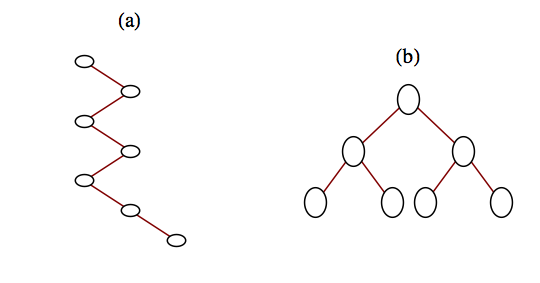
\includegraphics[width=0.9\linewidth]{images/fig-sol-10-4-5.png}
\caption*{\textbf{Figure 10.4.17:} }
\end{figure}
\end{divisionsolution}%
\begin{divisionsolution}{10.4.6.6}{}{exercise-431}%
\hypertarget{p-3753}{}%
Prove that the maximum number of vertices at level \(k\) of a binary tree is \(2^k\) and that a tree with that many vertices at level \(k\) must have  \(2^{k+1}-1\) vertices.%
\end{divisionsolution}%
\begin{divisionsolution}{10.4.6.7}{}{exercise-full-tree}%
\hypertarget{p-3754}{}%
Prove that if \(T\) is a full binary tree, then the number of leaves of \(T\) is one more than the number of internal vertices (non-leaves).%
\par\smallskip%
\noindent\textbf{Answer}.\quad%
\hypertarget{p-3755}{}%
Solution 1:%
\par
\hypertarget{p-3756}{}%
Basis: A binary tree consisting of a single vertex, which is a leaf, satisfies the equation \(\text{leaves} = \textrm{internal vertices} + 1\)%
\par
\hypertarget{p-3757}{}%
Induction:Assume that for some \(k\geq 1\), all full binary trees with \(k\) or fewer vertices have one more leaf than internal vertices. Now consider any full binary tree with \(k+1\) vertices. Let \(T_A\) and \(T_B\) be the left and right subtrees of the tree which, by the definition of a full binary tree, must both be full. If \(i_A\) and \(i_B\) are the numbers of internal vertices in \(T_A\) and \(T_B\), and \(j_A\) and \(j_B\) are the numbers of leaves, then \(j_A=i_A+1 \) and \(j_B=i_B+1\). Therefore, in the whole tree,%
\begin{equation*}
\begin{split}
\textrm{the number of leaves} & =j_A+j_B\\
&=\left(i_A+1\right)+\left(i_B+1\right)\\
&=\left(i_A+i_B+1\right)+1\\
&=(\textrm{number of internal vertices})+1
\end{split}
\end{equation*}
%
\par
\hypertarget{p-3758}{}%
Solution 2:%
\par
\hypertarget{p-3759}{}%
Imagine building a full binary tree starting with a single vertex. By continuing to add leaves in pairs so that the tree stays full, we can build any full binary tree. Our starting tree satisfies the condition that the number of leaves is one more than the number of internal vertices . By adding a pair of leaves to a full binary tree, an old leaf becomes an internal vertex, increasing the number of internal vertices by one. Although we lose a leaf, the two added leaves create a net increase of one leaf. Therefore, the desired equality is maintained.%
\end{divisionsolution}%
\chapter*{11 Algebraic Structures}
\addcontentsline{toc}{chapter}{11 Algebraic Structures}
\chaptermark{11 Algebraic Structures}
\section*{11.1 Operations}
\addcontentsline{toc}{section}{11.1 Operations}
\sectionmark{11.1 Operations}
\subsection*{11.1.4 Exercises for Section 11.1}
\addcontentsline{toc}{subsection}{11.1.4 Exercises for Section 11.1}
\begin{divisionsolution}{11.1.4.1}{}{exercise-433}%
\hypertarget{p-3795}{}%
Determine the properties that the following operations have on the positive integers.\leavevmode%
\begin{enumerate}[label=(\alph*)]
\item\hypertarget{li-1733}{}\hypertarget{p-3796}{}%
addition%
\item\hypertarget{li-1734}{}\hypertarget{p-3797}{}%
multiplication%
\item\hypertarget{li-1735}{}\hypertarget{p-3798}{}%
\(M\) defined by \(a M b = \textrm{ larger} \textrm{ of } a \textrm{ and} b\)%
\item\hypertarget{li-1736}{}\hypertarget{p-3799}{}%
\(m\) defined by \(a m b = \textrm{ smaller} \textrm{ of } a \textrm{ and } b\)%
\item\hypertarget{li-1737}{}\hypertarget{p-3800}{}%
@ defined by \(a @ b = a^b\)%
\end{enumerate}
%
\par\smallskip%
\noindent\textbf{Answer}.\quad%
\hypertarget{p-3801}{}%
\leavevmode%
\begin{enumerate}[label=(\alph*)]
\item\hypertarget{li-1738}{}\hypertarget{p-3802}{}%
Commutative, and associative. Notice that zero is the identity for addition, but it is not a positive integer.%
\item\hypertarget{li-1739}{}\hypertarget{p-3803}{}%
Commutative, associative, and has an  identity (1)%
\item\hypertarget{li-1740}{}\hypertarget{p-3804}{}%
Commutative, associative, has an identity (1), and is idempotent%
\item\hypertarget{li-1741}{}\hypertarget{p-3805}{}%
Commutative, associative, and idempotent%
\item\hypertarget{li-1742}{}\hypertarget{p-3806}{}%
None. Notice that   \(2 @ (3 @ 3) = 512\), while \((2 @ 3) @ 3 = 64\); and \(a @ 1 = a\), while \(1 @ a = 1\).%
\end{enumerate}
%
\end{divisionsolution}%
\begin{divisionsolution}{11.1.4.2}{}{exercise-434}%
\hypertarget{p-3807}{}%
Which pairs of operations in Exercise 1 are distributive over one another?%
\end{divisionsolution}%
\begin{divisionsolution}{11.1.4.3}{}{exercise-435}%
\hypertarget{p-3808}{}%
Let \(*\) be an operation on a set \(S\) and \(A, B \subseteq S\). Prove that if \(A\) and \(B\) are both closed under \(*\), then \(A\cap B\) is also closed under \(*\), but \(A \cup  B\) need not be.%
\par\smallskip%
\noindent\textbf{Answer}.\quad%
\hypertarget{p-3809}{}%
%
\begin{equation*}
\begin{split}
a, b \in  A \cap  B & \Rightarrow a, b \in  A \textrm{     by the definition of intersection}\\
& \Rightarrow  a*b \in A\textrm{      by the closure of } A \textrm{ with respect  to } *
\end{split}
\end{equation*}
Similarly, \(a, b \in  A \cap B \Rightarrow  a*b \in B\). Therefore, \(a * b \in  A \cap  B\). The set of positive integers is closed under addition, and so is the set of negative integers, but \(1 + -1 - 0\). Therefore, their union, the nonzero integers, is not closed under addition.%
\end{divisionsolution}%
\begin{divisionsolution}{11.1.4.4}{}{exercise-436}%
\hypertarget{p-3810}{}%
How can you pick out the identity of an operation from its table?%
\end{divisionsolution}%
\begin{divisionsolution}{11.1.4.5}{}{exercise-437}%
\hypertarget{p-3811}{}%
Define \(a * b\) by \(\lvert a - b \rvert\), the absolute value of \(a - b\). Which properties does \(*\) have on the set of natural numbers, \(\mathbb{N}\)?%
\par\smallskip%
\noindent\textbf{Answer}.\quad%
\hypertarget{p-3812}{}%
\leavevmode%
\begin{enumerate}[label=(\alph*)]
\item\hypertarget{li-1743}{}\hypertarget{p-3813}{}%
\(*\) is commutative since \(\left| a-b\right| =\left| b-a\right|\) for all \(a, b \in  \mathbb{N}\)%
\item\hypertarget{li-1744}{}\hypertarget{p-3814}{}%
\(*\) is not associative. Take \(a = 1\), \(b = 2\), and \(c = 3\), then \((a * b) * c =\left| \left| 1-2\right| -3\right| =2\) , and \(a * (b * c) = \left| 1-\left| 2-3\right| \right| = 0\).%
\item\hypertarget{li-1745}{}\hypertarget{p-3815}{}%
Zero is the identity for \(*\) on \(\mathbb{N}\), since \(a*0=\left| a - 0\right|  = a = \left| 0-a\right| = 0 * a.\)%
\item\hypertarget{li-1746}{}\hypertarget{p-3816}{}%
Each element of \(\mathbb{N}\) inverts itself since \(a * a=\left| a-a\right|  = 0\).%
\item\hypertarget{li-1747}{}\hypertarget{p-3817}{}%
\(*\) is not idempotent, since, for \(a\neq 0\), \(a * a =0 \neq a\).%
\end{enumerate}
%
\end{divisionsolution}%
\section*{11.2 Algebraic Systems}
\addcontentsline{toc}{section}{11.2 Algebraic Systems}
\sectionmark{11.2 Algebraic Systems}
\subsection*{11.2.4 Exercises for Section 11.2}
\addcontentsline{toc}{subsection}{11.2.4 Exercises for Section 11.2}
\begin{divisionsolution}{11.2.4.1}{}{exercise-438}%
\hypertarget{p-3851}{}%
Discuss the analogy between the terms generic and concrete for algebraic systems and the terms generic and trade for prescription drugs.%
\par\smallskip%
\noindent\textbf{Answer}.\quad%
\hypertarget{p-3852}{}%
The terms ``generic'' and ``trade'' for prescription drugs are analogous to ``generic'' and ``concrete'' algebraic systems. Generic aspirin, for example, has no name, whereas Bayer, Tylenol, Bufferin, and Anacin are all trade or specific types of aspirins. The same can be said of a generic group \([G; *]\) where \(G\) is a nonempty set and \(*\) is a binary operation on \(G\), When examples of typical domain elements can be given along with descriptions of how operations act on them, such as \(\mathbb{Q}\)\textasteriskcentered{} or \(M_{2\times 2}(\mathbb{R})\), then the system is concrete (has a specific name, as with the aspirin). Generic is a way to describe a general algebraic system, whereas a concrete system has a name or symbols making it distinguishable from other systems.%
\end{divisionsolution}%
\begin{divisionsolution}{11.2.4.2}{}{exercise-439}%
\hypertarget{p-3853}{}%
Discuss the connection between groups and monoids. Is every monoid a group? Is every group a monoid?%
\end{divisionsolution}%
\begin{divisionsolution}{11.2.4.3}{}{exercise-440}%
\hypertarget{p-3854}{}%
Which of the following are groups?\leavevmode%
\begin{enumerate}[label=(\alph*)]
\item\hypertarget{li-1759}{}\hypertarget{p-3855}{}%
\(B^*\) with concatenation (see Subsection~11.2.1).%
\item\hypertarget{li-1760}{}\hypertarget{p-3856}{}%
\(M_{2\times 3}(\mathbb{R})\) with matrix addition.%
\item\hypertarget{li-1761}{}\hypertarget{p-3857}{}%
\(M_{2\times 3}(\mathbb{R})\) with matrix multiplication.%
\item\hypertarget{li-1762}{}\hypertarget{p-3858}{}%
The positive real numbers, \(\mathbb{R}^+,\)with multiplication.%
\item\hypertarget{li-1763}{}\hypertarget{p-3859}{}%
The nonzero real numbers, \(\mathbb{R}^*\), with multiplication.%
\item\hypertarget{li-1764}{}\hypertarget{p-3860}{}%
\(\{1, -1\}\) with multiplication.%
\item\hypertarget{li-1765}{}\hypertarget{p-3861}{}%
The positive integers with the operation \(M\) defined by \(a M b = \textrm{ the larger of } a \textrm{ and } b\).%
\end{enumerate}
%
\par\smallskip%
\noindent\textbf{Answer}.\quad%
\hypertarget{p-3862}{}%
The systems in parts  b, d, e, and f are groups.%
\end{divisionsolution}%
\begin{divisionsolution}{11.2.4.4}{}{exercise-441}%
\hypertarget{p-3863}{}%
Prove that, \(\oplus\), defined by \(A \oplus  B = (A \cup  B) - (A \cap  B)\) is an associative operation on \(\mathcal{P}(U)\).%
\end{divisionsolution}%
\begin{divisionsolution}{11.2.4.5}{}{ex-rook-matrices}%
\hypertarget{p-3864}{}%
The following problem supplies an example of a non-abelian group. A rook matrix is a matrix that has only 0's and 1's as entries such that each row has exactly one 1 and each column has exactly one 1. The term rook matrix is derived from the fact that each rook matrix represents the placement of \(n\) rooks on an \(n\times n\) chessboard such that none of the rooks can attack one another. A rook in chess can move only vertically or horizontally, but not diagonally. Let \(R_n\) be the set of \(n\times n\) rook matrices. There are six \(3\times 3\) rook matrices: \(\begin{array}{ccc}
I=\left(
\begin{array}{ccc}
1 & 0 & 0 \\
0 & 1 & 0 \\
0 & 0 & 1 \\
\end{array}
\right) & R_1=\left(
\begin{array}{ccc}
0 & 1 & 0 \\
0 & 0 & 1 \\
1 & 0 & 0 \\
\end{array}
\right) & R_2=\left(
\begin{array}{ccc}
0 & 0 & 1 \\
1 & 0 & 0 \\
0 & 1 & 0 \\
\end{array}
\right) \\
F_1=\left(
\begin{array}{ccc}
1 & 0 & 0 \\
0 & 0 & 1 \\
0 & 1 & 0 \\
\end{array}
\right) & F_2=\left(
\begin{array}{ccc}
0 & 0 & 1 \\
0 & 1 & 0 \\
1 & 0 & 0 \\
\end{array}
\right) & F_3=\left(
\begin{array}{ccc}
0 & 1 & 0 \\
1 & 0 & 0 \\
0 & 0 & 1 \\
\end{array}
\right) \\
\end{array}\)\leavevmode%
\begin{enumerate}[label=(\alph*)]
\item\hypertarget{li-1766}{}\hypertarget{p-3865}{}%
List the \(2\times 2\) rook matrices. They form a group, \(R_2,\) under matrix multiplication. Write out the multiplication table. Is the group abelian?%
\item\hypertarget{li-1767}{}\hypertarget{p-3866}{}%
Write out the multiplication table for \(R_3\) . This is another group. Is it abelian?%
\item\hypertarget{li-1768}{}\hypertarget{p-3867}{}%
How many \(4\times 4\) rook matrices are there? How many \(n\times  n\) rook matrices are there?%
\end{enumerate}
%
\par\smallskip%
\noindent\textbf{Answer}.\quad%
\hypertarget{p-3868}{}%
\leavevmode%
\begin{enumerate}[label=(\alph*)]
\item\hypertarget{li-1769}{}\hypertarget{p-3869}{}%
Elements are \(I=\left(
\begin{array}{cc}
1 & 0 \\
0 & 1 \\
\end{array}
\right)\), and  \(T=\left(
\begin{array}{cc}
0 & 1 \\
1 & 0 \\
\end{array}
\right)\), the group is abelian.  Operation table is \(\begin{array}{c|cc}
\cdot & I  & T\\
\hline
I & I & T\\
T & T & I\\
\end{array}\)%
\item\hypertarget{li-1770}{}\hypertarget{p-3870}{}%
%
\begin{equation*}
\begin{array}{c|c}
& 
\begin{array}{cccccc}
I & R_1 & R_2 & F_1 & F_2 & F_3 \\
\end{array}
\\
\hline
\begin{array}{c}
I \\
R_1 \\
R_2 \\
F_1 \\
F_2 \\
F_3 \\
\end{array}
& 
\begin{array}{cccccc}
I & R_1 & R_2 & F_1 & F_2 & F_3 \\
R_1 & R_2 & I & F_2 & F_3 & F_1 \\
R_2 & I & R_1 & F_3 & F_1 & F_2 \\
F_1 & F & F_2 & I & R_2 & R_1 \\
F_2 & F_1 & F_3 & R_1 & I & R_2 \\
F_3 & F_2 & F_1 & R_2 & R_1 & I \\
\end{array}
\\
\end{array}
\end{equation*}
This group is non-abelian since, for example,  \(F_1 F_2=R_2\) and \(F_2 F_1=R_2\).%
\item\hypertarget{li-1771}{}\hypertarget{p-3871}{}%
4! = 24, \(n!\).%
\end{enumerate}
%
\end{divisionsolution}%
\begin{divisionsolution}{11.2.4.6}{}{exercise-443}%
\hypertarget{p-3872}{}%
For each of the following sets, identify the standard operation that results in a group. What is the identity of each group?\leavevmode%
\begin{enumerate}[label=(\alph*)]
\item\hypertarget{li-1772}{}\hypertarget{p-3873}{}%
The set of all \(2\times 2\) matrices with real entries and nonzero determinants.%
\item\hypertarget{li-1773}{}\hypertarget{p-3874}{}%
The set of \(2 \times  3\) matrices with rational entries.%
\end{enumerate}
%
\end{divisionsolution}%
\begin{divisionsolution}{11.2.4.7}{}{exercise-444}%
\hypertarget{p-3875}{}%
Let \(V = \{e,a,b, c\}\).  Let \(*\) be defined (partially) by \(x * x = e\) for all \(x \in  V\). Write a complete table for \(*\) so that \([V; * ]\) is a group.%
\par\smallskip%
\noindent\textbf{Answer}.\quad%
\hypertarget{p-3876}{}%
The identity is \(e\).   \(a*b = c\), \(a*c= b\),  \(b*c = a\), and \([V; *]\) is abelian. (This group is commonly called the Klein-4 group.)%
\end{divisionsolution}%
\section*{11.3 Some General Properties of Groups}
\addcontentsline{toc}{section}{11.3 Some General Properties of Groups}
\sectionmark{11.3 Some General Properties of Groups}
\subsection*{11.3.3 Exercises for Section 11.3}
\addcontentsline{toc}{subsection}{11.3.3 Exercises for Section 11.3}
\begin{divisionsolution}{11.3.3.1}{}{exercise-445}%
\hypertarget{p-3928}{}%
Let \([G; * ]\) be a group and \(a\) be an element of \(G\).  Define \(f:G \to  G\) by \(f(x) = a * x\).\leavevmode%
\begin{enumerate}[label=(\alph*)]
\item\hypertarget{li-1788}{}\hypertarget{p-3929}{}%
Prove that \(f\) is a bijection.%
\item\hypertarget{li-1789}{}\hypertarget{p-3930}{}%
On the basis of part a, describe a set of bijections on the set of integers.%
\end{enumerate}
%
\par\smallskip%
\noindent\textbf{Answer}.\quad%
\hypertarget{p-3931}{}%
\leavevmode%
\begin{enumerate}[label=(\alph*)]
\item\hypertarget{li-1790}{}\hypertarget{p-3932}{}%
\(f\) is injective:%
\begin{equation*}
\begin{split}
f(x) = f(y) & \Rightarrow  a * x = a * y \\
& \Rightarrow  x = y\textrm{       by left cancellation}\\
\end{split}\text{.}
\end{equation*}
%
\par
\hypertarget{p-3933}{}%
\(f\) is surjective:  For all \(b \in G\),   \(f(x) = b\) has the solution \(a^{-1}*b\).%
\item\hypertarget{li-1791}{}\hypertarget{p-3934}{}%
Functions of the form \(f(x) = a + x\), where \(a\) is any integer, are bijections%
\end{enumerate}
%
\end{divisionsolution}%
\begin{divisionsolution}{11.3.3.2}{}{exercise-446}%
\hypertarget{p-3935}{}%
Rephrase Theorem~11.3.3 and write out a clear proof.%
\end{divisionsolution}%
\begin{divisionsolution}{11.3.3.3}{}{exercise-447}%
\hypertarget{p-3936}{}%
Prove by induction on \(n\) that if \(a_1\), \(a_2,\ldots , a_n\) are elements of a group \(G\), \(n\geq 2\), then \(\left(a_1*a_2*\cdots *a_n\right)^{-1}= a_n^{-1}*\cdots *a_2^{-1}*a_1^{-1}\). Interpret this result in terms of \([\mathbb{Z}; +]\) and \([\mathbb{R}^*;\cdot]\).%
\par\smallskip%
\noindent\textbf{Answer}.\quad%
\hypertarget{p-3937}{}%
Basis: (\(n = 2\))   \(\left(a_1*a_2\right)^{-1}= a_2^{-1}*a_1^{-1}\) by Theorem~11.3.7.%
\par
\hypertarget{p-3938}{}%
Induction: Assume that for some \(n \geq  2\),%
\begin{equation*}
\left(a_1*a_2* \cdots *a_n\right)^{-1}=a_n^{-1}* \cdots * a_2^{-1}*a_1^{-1}
\end{equation*}
We must show that%
\begin{equation*}
\left(a_1*a_2* \cdots *a_n*a_{n+1}\right)^{-1}=a_{n+1}^{-1}*a_n^{-1}* \cdots * a_2^{-1}*a_1^{-1}
\end{equation*}
%
\par
\hypertarget{p-3939}{}%
This can be accomplished as follows:%
\begin{equation*}
\begin{split}
\left(a_1*a_2*\cdots *a_n*a_{n+1}\right)^{-1} &=\left(\left(a_1*a_2*\cdots *a_n\right)*a_{n+1}\right)^{-1}\textrm{  
by the associative law}\\
&=a_{n+1}^{-1}*\left(a_1*a_2*\cdots *a_n\right)^{-1}\textrm{      by the basis}\\
&=a_{n+1}^{-1}*\left(a_n^{-1}*\cdots * a_2^{-1}*a_1^{-1}\right) \textrm{   by the induction hypothesis}\\
&= a_{n+1}^{-1}*a_n^{-1}*\cdots * a_2^{-1}*a_1^{-1} \textrm{   by the associative law}\\
\end{split}
\end{equation*}
%
\end{divisionsolution}%
\begin{divisionsolution}{11.3.3.4}{}{exercise-448}%
\hypertarget{p-3940}{}%
True or false? If \(a\), \(b\), \(c\) are elements of a group \(G\), and \(a * b = c * a\), then \(b = c\). Explain your answer.%
\end{divisionsolution}%
\begin{divisionsolution}{11.3.3.5}{}{exercise-449}%
\hypertarget{p-3941}{}%
Prove Theorem~11.3.14.%
\par\smallskip%
\noindent\textbf{Answer}.\quad%
\hypertarget{p-3942}{}%
In this answer, we will refer to Lemma~11.3.13 simply as ``the lemma.''%
\par
\hypertarget{p-3943}{}%
\leavevmode%
\begin{enumerate}[label=(\alph*)]
\item\hypertarget{li-1792}{}\hypertarget{p-3944}{}%
Let \(p(n)\) be \(a^{-n}= \left(a^{-1}\right)^n\), where \(a\) is any element of group \([G; *]\). First we will prove that \(p(n)\) is true for all \(n \geq  0\).%
\par
\hypertarget{p-3945}{}%
Basis: If \(n = 0\), Using the definition of the zero exponent,  \(\left(a^0\right)^{-1} = e^{-1} = e\),  while \(\left(a^{-1}\right)^0= e\). Therefore, \(p(0)\) is true.%
\par
\hypertarget{p-3946}{}%
Induction: Assume that for some \(n \geq  0\), \(p(n\)) is true.%
\begin{equation*}
\begin{split}
\left(a^{n+1}\right)^{-1} &= \left(a^n*a\right)^{-1}\textrm{    by the definition of exponentiation}\\
& =a^{-1}*\left(a^n\right)^{-1}\textrm{       by the lemma}\\
& = a^{-1}*\left(a^{-1}\right)^n\textrm{      by the induction hypothesis}\\
& = \left(a^{-1}\right)^{n+1} \textrm{   by the lemma}	
\end{split}
\end{equation*}
%
\par
\hypertarget{p-3947}{}%
If \(n\) is negative, then \(-n\) is positive and%
\begin{equation*}
\begin{split}
a^{-n} & = \left(\left(\left(a^{-1}\right)^{-1}\right)^{-n} \right)\\
& =\left(a^{-1}\right)^{-(-n)}\textrm{    since the property is true for positive numbers}\\
& =\left(a^{-1}\right)^n
\end{split}
\end{equation*}
%
\item\hypertarget{li-1793}{}\hypertarget{p-3948}{}%
For \(m > 1\), let \(p(m)\) be \(a^{n+m}=a^n*a^m\) for all \(n\geq 1\). The basis for this proof follows directly from the basis for the definition of exponentiation.%
\par
\hypertarget{p-3949}{}%
Induction: Assume that for some \(m > 1\), \(p(m)\) is true. Then%
\begin{equation*}
\begin{split}
a^{n+(m+1)}&= a^{(n+m)+1}\textrm{      by the associativity of integer addition}\\
&=a^{n+m}*a^1\textrm{    by the definition of exponentiation}\\
&=\left(a^n*a^m\right)*a^1 \textrm{     by the induction hypothesis}\\
&= a^n*\left(a^m*a^1\right)\textrm{     by associativity}\\
&= a^n*a^{m+1}\textrm{    by the definition of exponentiation}
\end{split}
\end{equation*}
To complete the proof, you need to consider the cases where \(m\) and\slash{}or \(n\) are negative.%
\item\hypertarget{li-1794}{}\hypertarget{p-3950}{}%
Let \(p(m)\)be \(\left(a^n\right)^m= a^{n m}\) for all integers \(n\).%
\par
\hypertarget{p-3951}{}%
Basis: \(\left(a^m\right)^0= e\) and \(a^{m\cdot 0}=a^0= e\) therefore, \(p(0)\) is true.%
\par
\hypertarget{p-3952}{}%
Induction; Assume that \(p(m)\) is true for some \(m >\)0,%
\begin{equation*}
\begin{split}
\left(a^n\right)^{m+1}&=\left(a^n\right)^m*a^n \textrm{     by the definition of exponentiation}\\
&=a^{n m}*a^n\textrm{      by the induction hypothesis}\\
& =a^{n m + n}\textrm{      by part (b)  of this proof}\\
& =a^{n(m+1)}
\end{split}
\end{equation*}
Finally, if \(m\) is negative, we can verify that \(\left(a^n\right)^m= a^{n m}\) using many of the same steps as the positive case.%
\end{enumerate}
%
\end{divisionsolution}%
\begin{divisionsolution}{11.3.3.6}{}{exercise-450}%
\hypertarget{p-3953}{}%
Each of the following facts can be derived by identifying a certain group and then applying one of the theorems of this section to it. For each fact, list the group and the theorem that are used.\leavevmode%
\begin{enumerate}[label=(\alph*)]
\item\hypertarget{li-1795}{}\hypertarget{p-3954}{}%
\(\left(\frac{1}{3}\right)5\) is the only solution of \(3x = 5\).%
\item\hypertarget{li-1796}{}\hypertarget{p-3955}{}%
\(-(-(-18)) = -18\).%
\item\hypertarget{li-1797}{}\hypertarget{p-3956}{}%
If \(A, B, C\) are \(3\times 3\) matrices over the real numbers, with \(A + B = A + C\), then \(B = C\).%
\item\hypertarget{li-1798}{}\hypertarget{p-3957}{}%
There is only one subset of the natural numbers for which \(K \oplus  A = A\) for every \(A \subseteq N\).%
\end{enumerate}
%
\end{divisionsolution}%
\section*{11.4 Greatest Common Divisors  and the Integers Modulo \(n\)}
\addcontentsline{toc}{section}{11.4 Greatest Common Divisors  and the Integers Modulo \(n\)}
\sectionmark{11.4 Greatest Common Divisors  and the Integers Modulo \(n\)}
\subsection*{11.4.2 The Euclidean Algorithm}
\addcontentsline{toc}{subsection}{11.4.2 The Euclidean Algorithm}
\begin{investigationsolution}{11.4.1}{}{investigation-1}%
\hypertarget{p-3981}{}%
If you were allowed to pick two numbers less than 100, which would you pick in order to force Euclid to work hardest? Here's a hint:  The size of the quotient at each step determines how quickly the numbers decrease.%
\par\smallskip%
\noindent\textbf{Solution}.\quad%
\hypertarget{p-3982}{}%
If quotient in division is 1, then we get the slowest possible completion.   If \(a = b + r\), then working backwards, each remainder would be the sum of the two previous remainders.  This described a sequence like the Fibonacci sequence and indeed, the greatest common divisor of two consecutive Fibonacci numbers will take the most steps to reach a final value of 1.%
\end{investigationsolution}%
\subsection*{11.4.6 Exercises for Section 11.4}
\addcontentsline{toc}{subsection}{11.4.6 Exercises for Section 11.4}
\begin{divisionsolution}{11.4.6.1}{}{exercise-451}%
\hypertarget{p-4012}{}%
Determine the greatest common divisors of the following pairs of integers without using any computational assistance.\leavevmode%
\begin{enumerate}[label=(\alph*)]
\item\hypertarget{li-1808}{}\hypertarget{p-4013}{}%
\(2^3 \cdot 3^2\cdot 5\)   and  \(2^2 \cdot 3 \cdot 5^2\cdot 7\)%
\item\hypertarget{li-1809}{}\hypertarget{p-4014}{}%
\(7! \)  and  \(3\cdot 5\cdot 7\cdot 9\cdot 11\cdot 13\)%
\item\hypertarget{li-1810}{}\hypertarget{p-4015}{}%
\(19^4\)  and  \(19^5\)%
\item\hypertarget{li-1811}{}\hypertarget{p-4016}{}%
12112 and 0%
\end{enumerate}
%
\par\smallskip%
\noindent\textbf{Answer}.\quad%
\hypertarget{p-4017}{}%
\leavevmode%
\begin{enumerate}[label=(\alph*)]
\item\hypertarget{li-1812}{}\hypertarget{p-4018}{}%
\(2^2 \cdot 3 \cdot 5\)%
\item\hypertarget{li-1813}{}\hypertarget{p-4019}{}%
\(3^2 \cdot 5\cdot 7\)%
\item\hypertarget{li-1814}{}\hypertarget{p-4020}{}%
\(19^4\)%
\item\hypertarget{li-1815}{}\hypertarget{p-4021}{}%
12112%
\end{enumerate}
%
\end{divisionsolution}%
\begin{divisionsolution}{11.4.6.2}{}{exercise-452}%
\hypertarget{p-4022}{}%
Find all possible values of the following, assuming that \(m\) is a positive integer.\leavevmode%
\begin{enumerate}[label=(\alph*)]
\item\hypertarget{li-1816}{}\hypertarget{p-4023}{}%
\(\gcd(m+1,m)\)%
\item\hypertarget{li-1817}{}\hypertarget{p-4024}{}%
\(\gcd(m+2,m)\)%
\item\hypertarget{li-1818}{}\hypertarget{p-4025}{}%
\(\gcd(m+4,m)\)%
\end{enumerate}
%
\end{divisionsolution}%
\begin{divisionsolution}{11.4.6.3}{}{exercise-453}%
\hypertarget{p-4026}{}%
Calculate:\leavevmode%
\begin{multicols}{2}
\begin{enumerate}[label=(\alph*)]
\item\hypertarget{li-1819}{}\hypertarget{p-4027}{}%
\(7 +_8 3\)%
\item\hypertarget{li-1820}{}\hypertarget{p-4028}{}%
\(7 \times_8 3\)%
\item\hypertarget{li-1821}{}\hypertarget{p-4029}{}%
\(4\times_8 4\)%
\item\hypertarget{li-1822}{}\hypertarget{p-4030}{}%
\(10+_{12} 2\)%
\item\hypertarget{li-1823}{}\hypertarget{p-4031}{}%
\(6\times_8 2 +_8 6\times_8 5 \)%
\item\hypertarget{li-1824}{}\hypertarget{p-4032}{}%
\(6\times_8 \left(2 +_85\right)\)%
\item\hypertarget{li-1825}{}\hypertarget{p-4033}{}%
\(3 \times_5  3 \times_5  3 \times_5  3 \equiv  3^4 (\textrm{ mod} 5)\)%
\item\hypertarget{li-1826}{}\hypertarget{p-4034}{}%
\(2 \times_{11}7\)%
\item\hypertarget{li-1827}{}\hypertarget{p-4035}{}%
\(2 \times_{14}7\)%
\end{enumerate}
\end{multicols}
%
\par\smallskip%
\noindent\textbf{Answer}.\quad%
\hypertarget{p-4036}{}%
\leavevmode%
\begin{multicols}{4}
\begin{enumerate}[label=(\alph*)]
\item\hypertarget{li-1828}{}\hypertarget{p-4037}{}%
2%
\item\hypertarget{li-1829}{}\hypertarget{p-4038}{}%
5%
\item\hypertarget{li-1830}{}\hypertarget{p-4039}{}%
0%
\item\hypertarget{li-1831}{}\hypertarget{p-4040}{}%
0%
\item\hypertarget{li-1832}{}\hypertarget{p-4041}{}%
2%
\item\hypertarget{li-1833}{}\hypertarget{p-4042}{}%
2%
\item\hypertarget{li-1834}{}\hypertarget{p-4043}{}%
1%
\item\hypertarget{li-1835}{}\hypertarget{p-4044}{}%
3%
\item\hypertarget{li-1836}{}\hypertarget{p-4045}{}%
0%
\end{enumerate}
\end{multicols}
%
\end{divisionsolution}%
\begin{divisionsolution}{11.4.6.4}{}{exercise-454}%
\hypertarget{p-4046}{}%
List the additive inverses of the following elements:\leavevmode%
\begin{enumerate}[label=(\alph*)]
\item\hypertarget{li-1837}{}\hypertarget{p-4047}{}%
4, 6, 9 in \(\mathbb{Z}_{10}\)%
\item\hypertarget{li-1838}{}\hypertarget{p-4048}{}%
16, 25, 40 in \(\mathbb{Z}_{50}\)%
\end{enumerate}
%
\end{divisionsolution}%
\begin{divisionsolution}{11.4.6.5}{}{exercise-455}%
\hypertarget{p-4049}{}%
In the group \(\mathbb{Z}_{11}\) , what are:\leavevmode%
\begin{enumerate}[label=(\alph*)]
\item\hypertarget{li-1839}{}\hypertarget{p-4050}{}%
3(4)?%
\item\hypertarget{li-1840}{}\hypertarget{p-4051}{}%
36(4)?%
\item\hypertarget{li-1841}{}\hypertarget{p-4052}{}%
How could you efficiently compute \(m(4)\), \(m \in  \mathbb{Z}\)?%
\end{enumerate}
%
\par\smallskip%
\noindent\textbf{Answer}.\quad%
\hypertarget{p-4053}{}%
\leavevmode%
\begin{multicols}{2}
\begin{enumerate}[label=(\alph*)]
\item\hypertarget{li-1842}{}\hypertarget{p-4054}{}%
1%
\item\hypertarget{li-1843}{}\hypertarget{p-4055}{}%
1%
\item\hypertarget{li-1844}{}\hypertarget{p-4056}{}%
\(m(4) = r(4)\), where \(m = 11 q + r\), \(0 \leq  r < 11\)%
\end{enumerate}
\end{multicols}
%
\end{divisionsolution}%
\begin{divisionsolution}{11.4.6.6}{}{exercise-456}%
\hypertarget{p-4057}{}%
Prove that \(\{1, 2, 3, 4\}\) is a group under the operation \(\times_5 \).%
\end{divisionsolution}%
\begin{divisionsolution}{11.4.6.7}{}{exercise-457}%
\hypertarget{p-4058}{}%
A student is asked to solve the following equations under the requirement that all arithmetic should be done in \(\mathbb{Z}_2\). List all solutions.\leavevmode%
\begin{enumerate}[label=(\alph*)]
\item\hypertarget{li-1845}{}\hypertarget{p-4059}{}%
\(x^2 + 1 = 0\).%
\item\hypertarget{li-1846}{}\hypertarget{p-4060}{}%
\(x^2 + x + 1 = 0\).%
\end{enumerate}
%
\par\smallskip%
\noindent\textbf{Answer}.\quad%
\hypertarget{p-4061}{}%
Since the solutions, if they exist, must come from \(\mathbb{Z}_2\), substitution is the easiest approach.\leavevmode%
\begin{enumerate}[label=(\alph*)]
\item\hypertarget{li-1847}{}\hypertarget{p-4062}{}%
1 is the only solution, since  \(1^2+_21=0\)   and  \(0^2+_21=1\)%
\item\hypertarget{li-1848}{}\hypertarget{p-4063}{}%
No solutions, since \(0^2+_2 0+_2 1=1\), and  \(1^2+_2 1+_2 1=1\)%
\end{enumerate}
%
\end{divisionsolution}%
\begin{divisionsolution}{11.4.6.8}{}{exercise-458}%
\hypertarget{p-4064}{}%
Determine the solutions of the same equations as in Exercise 5 in \(\mathbb{Z}_5\).%
\end{divisionsolution}%
\begin{divisionsolution}{11.4.6.9}{}{exercise_u_n}%
\hypertarget{p-4065}{}%
\leavevmode%
\begin{enumerate}[label=(\alph*)]
\item\hypertarget{li-1849}{}\hypertarget{p-4066}{}%
Write out the operation table for \(\times_8\) on \(\{1,3,5,7\}\), and convince your self that this is a group.%
\item\hypertarget{li-1850}{}\hypertarget{p-4067}{}%
Let \(\mathbb{U}_{n}\) be the elements of \(\mathbb{Z}_{n}\) that have inverses with respect to \(\times_{n}\).  Convince yourself that \(\mathbb{U}_{n}\) is a group under \(\times_{n}\).%
\item\hypertarget{li-1851}{}\hypertarget{p-4068}{}%
Prove that the elements of \(\mathbb{U}_{n}\)  are those elements  \(a\in \mathbb{Z}_{n} \) such that \(\gcd(n,a)=1\).  You may use  Theorem~11.4.9 in this proof.%
\end{enumerate}
%
\end{divisionsolution}%
\begin{divisionsolution}{11.4.6.10}{}{exercise-460}%
\hypertarget{p-4069}{}%
Prove the division property, Theorem~11.4.1.%
\par\smallskip%
\noindent\textbf{Hint}.\quad%
\hypertarget{p-4070}{}%
Prove by induction on \(m\) that you can divide any positive integer into \(m\). That is, let \(p(m)\) be ``For all \(n\) greater than zero, there exist unique integers \(q\) and \(r\) such that \(\dots\) .''  In the induction step, divide \(n\) into \(m - n\).%
\end{divisionsolution}%
\begin{divisionsolution}{11.4.6.11}{}{exercise-461}%
\hypertarget{p-4071}{}%
Suppose \(f:\mathbb{Z}_{17}\to \mathbb{Z}_{17}\) such \(f(i)=a \times_{17} i +_{17} b \) where \(a\) and \(b\) are integer constants. Furthermore,  assume that \(f(1)=11\) and \(f(2)=4\). Find a formula for \(f(i)\) and also find a formula for the inverse of \(f\).%
\par\smallskip%
\noindent\textbf{Solution}.\quad%
\hypertarget{p-4072}{}%
The given conditions can be converted to a system of linear equations:%
\begin{equation*}
\begin{array}{c}
f(1)=11 \Rightarrow   a +_{17} b = 11\\
f(2)=4  \Rightarrow  2 \times_{17} a +_{17} b =4\\
\end{array}
\end{equation*}
%
\par
\hypertarget{p-4073}{}%
If we subtract the first equation from the second, we get  \(a = 4 +_{17} (-11) = 4 +_{17} 6= 10\).  This implies that \(b=1\), and \(f(i) = 10\times+{17}i + 1\).  To get a formula for the inverse of \(f\) we solve \(f(j)=i\) for \(j\), using the fact that the multiplicative inverse of 10 (mod 17) is 12.%
\begin{equation*}
\begin{split}
f(j)=i & \Rightarrow 10\times+{17}j + 1 = i\\
& \Rightarrow    10\times+{17}j  = i +_{17} 16\\
& \Rightarrow     j = 12\times_{17}( i +_{17} 16)\\
\end{split}
\end{equation*}
Therefore  \(f^{-1}(i) = 12\times_{17}( i +_{17} 16) = 12\times_{17} i +_{17} 5\).%
\end{divisionsolution}%
\section*{11.5 Subsystems}
\addcontentsline{toc}{section}{11.5 Subsystems}
\sectionmark{11.5 Subsystems}
\subsection*{11.5.5 Exercises for Section 11.5}
\addcontentsline{toc}{subsection}{11.5.5 Exercises for Section 11.5}
\begin{divisionsolution}{11.5.5.1}{}{exercise-462}%
\hypertarget{p-4113}{}%
Which of the following subsets of the real numbers is a subgroup of \([\mathbb{R}; +]\)?\leavevmode%
\begin{enumerate}[label=(\alph*)]
\item\hypertarget{li-1866}{}\hypertarget{p-4114}{}%
the rational numbers%
\item\hypertarget{li-1867}{}\hypertarget{p-4115}{}%
the positive real numbers%
\item\hypertarget{li-1868}{}\hypertarget{p-4116}{}%
\(\{k/2 \mid k \textrm{ is} \textrm{ an} \textrm{ integer}\}\)%
\item\hypertarget{li-1869}{}\hypertarget{p-4117}{}%
\(\{2^k  \mid k \textrm{ is an  integer}\}\)%
\item\hypertarget{li-1870}{}\hypertarget{p-4118}{}%
\(\{x \mid -100 \leq x \leq  100\}\)%
\end{enumerate}
%
\par\smallskip%
\noindent\textbf{Answer}.\quad%
\hypertarget{p-4119}{}%
Only  a and c are subgroups.%
\end{divisionsolution}%
\begin{divisionsolution}{11.5.5.2}{}{exercise-463}%
\hypertarget{p-4120}{}%
Describe in simpler terms the following subgroups of \(\mathbb{Z}\):\leavevmode%
\begin{enumerate}[label=(\alph*)]
\item\hypertarget{li-1871}{}\hypertarget{p-4121}{}%
\(5\mathbb{Z} \cap  4\mathbb{Z}\)%
\item\hypertarget{li-1872}{}\hypertarget{p-4122}{}%
\(4\mathbb{Z} \cap  6\mathbb{Z}\) (be careful)%
\item\hypertarget{li-1873}{}\hypertarget{p-4123}{}%
the only finite subgroup of \(\mathbb{Z}\)%
\end{enumerate}
%
\end{divisionsolution}%
\begin{divisionsolution}{11.5.5.3}{}{exercise-464}%
\hypertarget{p-4124}{}%
Find at least two proper subgroups of \(R_3\) , the set of \(3\times 3\) rook matrices (see Exercise~11.2.4.5).%
\par\smallskip%
\noindent\textbf{Answer}.\quad%
\hypertarget{p-4125}{}%
\(\left\{I,R_1,R_2\right\}\), \(\left\{I,F_1\right\}\), \(\left\{I,F_2\right\}\), and \(\left\{I,F_3\right\}\) are all the proper subgroups of \(R_3\).%
\end{divisionsolution}%
\begin{divisionsolution}{11.5.5.4}{}{exercise-465}%
\hypertarget{p-4126}{}%
Where should you place the following in Figure~11.5.12?\leavevmode%
\begin{enumerate}[label=(\alph*)]
\item\hypertarget{li-1874}{}\hypertarget{p-4127}{}%
\(e\)%
\item\hypertarget{li-1875}{}\hypertarget{p-4128}{}%
\(a^{-1}\)%
\item\hypertarget{li-1876}{}\hypertarget{p-4129}{}%
\(x * y\)%
\end{enumerate}
%
\begin{figure}
\centering
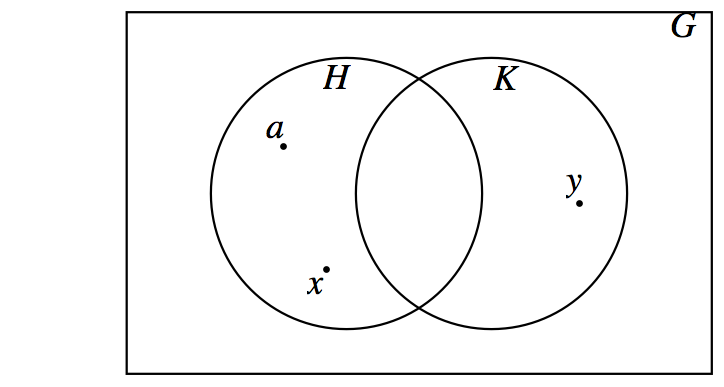
\includegraphics[width=0.67\linewidth]{images/fig-venn-subgroups.png}
\caption*{\textbf{Figure 11.5.12:} Figure for exercise 4}
\end{figure}
\end{divisionsolution}%
\begin{divisionsolution}{11.5.5.5}{}{exercise-466}%
\hypertarget{p-4130}{}%
\leavevmode%
\begin{enumerate}[label=(\alph*)]
\item\hypertarget{li-1877}{}\hypertarget{p-4131}{}%
List the cyclic subgroups of \(\mathbb{Z}_6\) and draw an ordering diagram for the relation ``is a subset of'' on these subgroups.%
\item\hypertarget{li-1878}{}\hypertarget{p-4132}{}%
Do the same for \(\mathbb{Z}_{12}\).%
\item\hypertarget{li-1879}{}\hypertarget{p-4133}{}%
Do the same for \(\mathbb{Z}_8\).%
\item\hypertarget{li-1880}{}\hypertarget{p-4134}{}%
On the basis of your results in parts a, b, and c, what would you expect if you did the same with \(\mathbb{Z}_{24}\)?%
\end{enumerate}
%
\par\smallskip%
\noindent\textbf{Answer}.\quad%
\hypertarget{p-4135}{}%
\leavevmode%
\begin{enumerate}[label=(\alph*)]
\item\hypertarget{li-1881}{}\hypertarget{p-4136}{}%
\(\langle 1\rangle  = \langle 5\rangle  = \mathbb{Z}_6\), \(\quad\)\(\langle 2\rangle = \langle 4\rangle  = \{2, 4, 0\}\), \(\langle 3\rangle = \{3, 0\}\), \(\langle 0\rangle  = \{0\}\)%
\item\hypertarget{li-1882}{}\hypertarget{p-4137}{}%
\(\langle 1\rangle  = \langle 5\rangle  = \langle 7\rangle  = \langle 11\rangle  =\mathbb{Z}_{12}\), \(\langle 2\rangle = \langle 10\rangle  = \{2, 4, 6, 8, 10, 0\}\), \(\langle 3\rangle = \langle 9\rangle  = \{3, 6, 9, 0\}\), \(\langle 4\rangle = \langle  8 \rangle  = \{ 4 , 8, 0\}\), \(\langle 6\rangle  = \{6, 0\}\), \(\langle 0\rangle  = \{0\}\)%
\item\hypertarget{li-1883}{}\hypertarget{p-4138}{}%
\(\langle 1\rangle  = \langle  3\rangle  = \langle  5 \rangle  = \langle 7\rangle  = \mathbb{Z}_8\), \(\langle 2\rangle  = \langle 6\rangle  = \{2, 4, 6, 0\}\), \(\langle 4\rangle  = \{4, 0\}\), \(\langle 0\rangle  = \{0\}\)%
\item\hypertarget{li-1884}{}\hypertarget{p-4139}{}%
Based on the ordering diagrams for parts a through c in Figure~11.5.13, we would expect to see an ordering diagram similar to the one for divides on \(\{1, 2, 3,
4, 6, 8, 12, 24\}\) (the divisors of 24) if we were to examine the subgroups of \(\mathbb{Z}_{24}\). This is indeed the case.%
\end{enumerate}
%
\begin{figure}
\centering
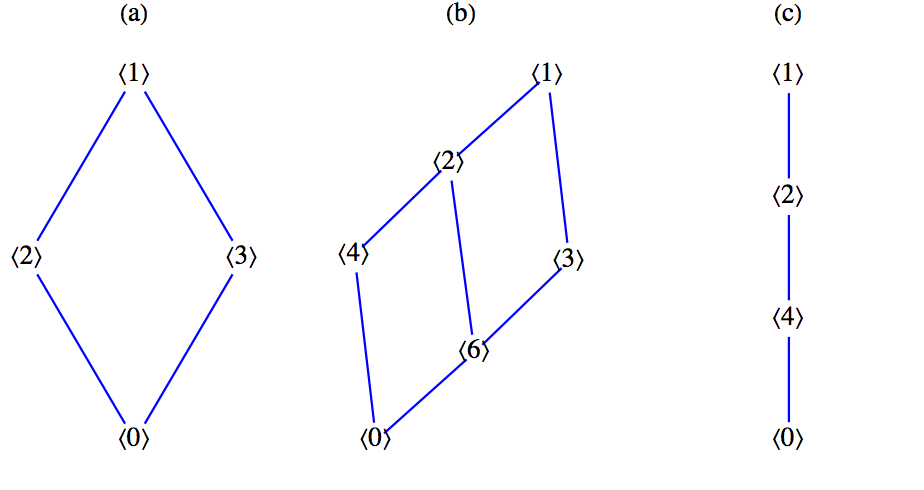
\includegraphics[width=0.75\linewidth]{images/fig-sol-11-5-5.png}
\caption*{\textbf{Figure 11.5.13:} Figure for exercise 5}
\end{figure}
\end{divisionsolution}%
\begin{divisionsolution}{11.5.5.6}{Subgroups generated by subsets of a group.}{exercise-467}%
\hypertarget{p-4140}{}%
The concept of a cyclic subgroup is a special case of the concept that we will discuss here. Let \([G; * ]\) be a group and \(S\) a nonempty subset of \(G\). Define the set \(\langle S \rangle\) recursively by:\leavevmode%
\begin{itemize}[label=\textbullet]
\item{}\hypertarget{p-4141}{}%
If \(a\in S\), then \(a\in  \langle S \rangle\).%
\item{}\hypertarget{p-4142}{}%
If \(a, b \in \langle S \rangle\), then \(a * b \in \langle S \rangle\), and%
\item{}\hypertarget{p-4143}{}%
If \(a \in \langle S \rangle\), then \(a^{-1}\in \langle S \rangle\).%
\end{itemize}
%
\par
\hypertarget{p-4144}{}%
\leavevmode%
\begin{enumerate}[label=(\alph*)]
\item\hypertarget{li-1888}{}\hypertarget{p-4145}{}%
By its definition, \(\langle S \rangle\)  has all of the properties needed to be a subgroup of \(G\). The only thing that isn't obvious is that the identity of \(G\) is in \(\langle S \rangle\).  Prove that the identity of \(G\) is in \(\langle S \rangle\).%
\item\hypertarget{li-1889}{}\hypertarget{p-4146}{}%
What is \(\langle\{9, 15\}\rangle\) in\([\mathbb{Z}; +]\)?%
\item\hypertarget{li-1890}{}\hypertarget{p-4147}{}%
Prove that if \(H \leq  G\) and \(S \subseteq  H\), then \(\langle S \rangle\leq H\). This proves that \(\langle S \rangle\) is contained in every subgroup of \(G\) that contains \(S\); that is, \(\langle S \rangle =\underset{S\subseteq H, H\leq G}{\cap }H\).%
\item\hypertarget{li-1891}{}\hypertarget{p-4148}{}%
Describe \(\langle \{0.5, 3\}\rangle \) in \(\left[ \mathbb{R}^+;\cdot \right]\) and in \([\mathbb{R}; +]\).%
\item\hypertarget{li-1892}{}\hypertarget{p-4149}{}%
If \(j, k \in  \mathbb{Z}\), \(\langle\{j,k\}\rangle\) is a cyclic subgroup of \(\mathbb{Z}\). In terms of \(j\) and \(k\), what is a generator of \(\langle \{j, k\}\rangle \)?%
\end{enumerate}
%
\end{divisionsolution}%
\begin{divisionsolution}{11.5.5.7}{}{exercise-468}%
\hypertarget{p-4150}{}%
Prove that if \(H,K \leq  G\), and \(H\cup K=G\), then \(H = G\) or \(K = G\).%
\par\smallskip%
\noindent\textbf{Hint}.\quad%
\hypertarget{p-4151}{}%
Use an indirect argument.%
\par\smallskip%
\noindent\textbf{Answer}.\quad%
\hypertarget{p-4152}{}%
Assume that \(H\) and \(K\) are subgroups of group \(G\), and that, as in Figure~11.5.12, there are elements \(x \in  H - K\) and \(y \in  K - H\). Consider the product \(x * y\). Where could it be placed in the Venn diagram? If we can prove that it must lie in the outer region, \(H^c \cap K^c=(H \cup K)^c\), then we have proven that \(H \cup  K\) is not closed under \(*\) and cannot be a subgroup of \(G\), Assume that  \(x*y\in H\).  Since \(x\) is in  \(H\),  \(x^{-1}\) is in \(H\) and so by closure \(x^{-1}*(x * y )= y \in H\) which is a contradiction.   Similarly, \(x*y \notin K\).%
\par
\hypertarget{p-4153}{}%
One way to interpret this theorem is that no group is the union of two groups.%
\end{divisionsolution}%
\begin{divisionsolution}{11.5.5.8}{}{exercise-469}%
\hypertarget{p-4154}{}%
Prove that the order of an element, \(a\) of a group is the least positive integer, \(k\), such that \(a^k\) is the identity of the group.%
\end{divisionsolution}%
\section*{11.6 Direct Products}
\addcontentsline{toc}{section}{11.6 Direct Products}
\sectionmark{11.6 Direct Products}
\subsection*{11.6.3 Exercises for Section 11.6}
\addcontentsline{toc}{subsection}{11.6.3 Exercises for Section 11.6}
\begin{divisionsolution}{11.6.3.1}{}{exercise-470}%
\hypertarget{p-4195}{}%
Write out the group table of \(\mathbb{Z}_2 \times  \mathbb{Z}_3\) and find the two proper subgroups of this group.%
\par\smallskip%
\noindent\textbf{Answer}.\quad%
\hypertarget{p-4196}{}%
Table of \(\mathbb{Z}_2\times  \mathbb{Z}_3\):%
\begin{equation*}
\begin{array}{c|cccccc}
+&(0,0)&(0,1)&(0,2)&(1,0)&(1,1)&(1,2)\\
\hline
(0,0)&(0,0)&(0,1)&(0,2)&(1,0)&(1,1)&(1,2)\\
(0,1)&(0,1)&(0,2)&(0,0)&(1,1)&(1,2)&(1,0)\\
(0,2)&(0,2)&(0,0)&(0,1)&(1,2)&(1,0)&(1,1)\\
(1,0)&(1,0)&(1,1)&(1,2)&(0,0)&(0,1)&(0,2)\\
(1,1)&(1,1)&(1,2)&(1,0)&(0,1)&(0,2)&(0,0)\\
(1,2)&(1,2)&(1,0)&(1,1)&(0,2)&(0,0)&(0,1)
\end{array}
\end{equation*}
The only two proper subgroups are \(\{(0, 0), (1, 0)\}\) and \(\{(0, 0), (0, 1), (0, 2)\}\)%
\end{divisionsolution}%
\begin{divisionsolution}{11.6.3.2}{}{exercise-471}%
\hypertarget{p-4197}{}%
List more examples of proper subgroups of \(\mathbb{R}^2\) that are different from the ones listed in this section.%
\end{divisionsolution}%
\begin{divisionsolution}{11.6.3.3}{Algebraic properties of the \(n\)-cube.}{exercise-n-cube-algebra}%
\hypertarget{p-4198}{}%
\leavevmode%
\begin{enumerate}[label=(\alph*)]
\item\hypertarget{li-1909}{}\hypertarget{p-4199}{}%
The four elements of \(\mathbb{Z}_2^2\) can be visualized geometrically as the four corners of the 2-cube.  Algebraically describe the statements:%
\begin{enumerate}[label=(\roman*)]
\item\hypertarget{li-1910}{}\hypertarget{p-4200}{}%
Corners \(a\) and \(b\) are adjacent.%
\item\hypertarget{li-1911}{}\hypertarget{p-4201}{}%
Corners \(a\) and \(b\) are diagonally opposite one another.%
\end{enumerate}
%
\item\hypertarget{li-1912}{}\hypertarget{p-4202}{}%
The eight elements of \(\mathbb{Z}_2{}^3\) can be visualized as the eight corners of the 3-cube. One face contains \(\mathbb{Z}_2 \times 
\mathbb{Z}_2\times \{0\}\) and the opposite face contains the remaining four elements so that \((a, b, 1)\) is behind \((a, b, 0)\). As in part a, describe statements i and ii algebraically.%
\item\hypertarget{li-1913}{}\hypertarget{p-4203}{}%
If you could imagine a geometric figure similar to the square or cube in \(n\) dimensions, and its comers were labeled by elements of \(\mathbb{Z}_2{}^n\) as in parts a and b, how would statements i and ii be expressed algebraically?%
\end{enumerate}
%
\par\smallskip%
\noindent\textbf{Answer}.\quad%
\hypertarget{p-4204}{}%
\leavevmode%
\begin{enumerate}[label=(\alph*)]
\item\hypertarget{li-1914}{}\hypertarget{p-4205}{}%
(i) \(a + b \textrm{ could  be }(1, 0) \textrm{ or } (0, 1)\). (ii)  \(a + b = (1, 1)\).%
\item\hypertarget{li-1915}{}\hypertarget{p-4206}{}%
(i) \(a + b \textrm{ could  be}(1, 0, 0), (0, 1, 0), \textrm{ or }(0, 0, 1)\). (ii) \(a + b = (1, 1, 1)\).%
\item\hypertarget{li-1916}{}\hypertarget{p-4207}{}%
(i) \(a + b\) has exactly one 1. (ii) \(a + b\) has all \(1's\).%
\end{enumerate}
%
\end{divisionsolution}%
\begin{divisionsolution}{11.6.3.4}{}{exercise-473}%
\hypertarget{p-4208}{}%
\leavevmode%
\begin{enumerate}[label=(\alph*)]
\item\hypertarget{li-1917}{}\hypertarget{p-4209}{}%
Suppose that you were to be given a group \([G; * ]\) and asked to solve the equation \(x * x = e\). Without knowing the group, can you anticipate how many solutions there will be?%
\item\hypertarget{li-1918}{}\hypertarget{p-4210}{}%
Answer the same question as part a for the equation \(x * x = x\).%
\end{enumerate}
%
\end{divisionsolution}%
\begin{divisionsolution}{11.6.3.5}{}{exercise-474}%
\hypertarget{p-4211}{}%
Which of the following sets are subgroups of \(\mathbb{Z} \times  \mathbb{Z}\)? Give a reason for any negative answers.\leavevmode%
\begin{enumerate}[label=(\alph*)]
\item\hypertarget{li-1919}{}\hypertarget{p-4212}{}%
\(\{0\}\)%
\item\hypertarget{li-1920}{}\hypertarget{p-4213}{}%
\(\{(2j, 2k) \mid j,k\in  \mathbb{Z}\}\)%
\item\hypertarget{li-1921}{}\hypertarget{p-4214}{}%
\(\{(2j+ 1, 2k) \mid j,k\in \mathbb{Z}\}\)%
\item\hypertarget{li-1922}{}\hypertarget{p-4215}{}%
\(\{(n, n^2 ) \mid n \in \mathbb{Z}\}\)%
\item\hypertarget{li-1923}{}\hypertarget{p-4216}{}%
\(\{(j, k) \mid j + k\textrm{ is} \textrm{ even}\}\)%
\end{enumerate}
%
\par\smallskip%
\noindent\textbf{Answer}.\quad%
\hypertarget{p-4217}{}%
\leavevmode%
\begin{enumerate}[label=(\alph*)]
\item\hypertarget{li-1924}{}\hypertarget{p-4218}{}%
No,  0 is not an element of \(\mathbb{Z} \times \mathbb{Z}\).%
\item\hypertarget{li-1925}{}\hypertarget{p-4219}{}%
Yes.%
\item\hypertarget{li-1926}{}\hypertarget{p-4220}{}%
No, (0, 0) is not an element of this set.%
\item\hypertarget{li-1927}{}\hypertarget{p-4221}{}%
No, the set is not closed: \((1, 1) + (2, 4) = (3, 5)\) and \((3, 5)\) is not in the set.%
\item\hypertarget{li-1928}{}\hypertarget{p-4222}{}%
Yes.%
\end{enumerate}
%
\end{divisionsolution}%
\begin{divisionsolution}{11.6.3.6}{}{exercise-475}%
\hypertarget{p-4223}{}%
Determine the following values in the group \(\mathbb{Z}_3 \times  \mathbb{R}^*\):\leavevmode%
\begin{enumerate}[label=(\alph*)]
\item\hypertarget{li-1929}{}\hypertarget{p-4224}{}%
\((2,1)* (1,2)\)%
\item\hypertarget{li-1930}{}\hypertarget{p-4225}{}%
the identity element%
\item\hypertarget{li-1931}{}\hypertarget{p-4226}{}%
\((1, 1/2)^{-1}\)%
\end{enumerate}
%
\end{divisionsolution}%
\section*{11.7 Isomorphisms}
\addcontentsline{toc}{section}{11.7 Isomorphisms}
\sectionmark{11.7 Isomorphisms}
\subsection*{11.7.3 Exercises for Section 11.7}
\addcontentsline{toc}{subsection}{11.7.3 Exercises for Section 11.7}
\begin{divisionsolution}{11.7.3.1}{}{exercise-476}%
\hypertarget{p-4259}{}%
State whether each pair of groups below is isomorphic. For each pair that is, give an isomorphism; for those that are not, give your reason.\leavevmode%
\begin{enumerate}[label=(\alph*)]
\item\hypertarget{li-1944}{}\hypertarget{p-4260}{}%
\(\mathbb{Z} \times  \mathbb{R}\) and \(\mathbb{R} \times  \mathbb{Z}\)%
\item\hypertarget{li-1945}{}\hypertarget{p-4261}{}%
\(\mathbb{Z}_2\times \mathbb{Z}\)  and \(\mathbb{Z} \times  \mathbb{Z}\)%
\item\hypertarget{li-1946}{}\hypertarget{p-4262}{}%
\(\mathbb{R}\) and \(\mathbb{Q} \times  \mathbb{Q}\)%
\item\hypertarget{li-1947}{}\hypertarget{p-4263}{}%
\(\mathcal{P}(\{1, 2\})\) with symmetric difference and \(\mathbb{Z}_2{}^2\)%
\item\hypertarget{li-1948}{}\hypertarget{p-4264}{}%
\(\mathbb{Z}_2{}^2\) and \(\mathbb{Z}_4\)%
\item\hypertarget{li-1949}{}\hypertarget{p-4265}{}%
\(\mathbb{R}^4\) and \(M_{2\times 2}(\mathbb{R})\) with matrix addition%
\item\hypertarget{li-1950}{}\hypertarget{p-4266}{}%
\(\mathbb{R}^2\) and \(\mathbb{R} \times  \mathbb{R}^+\)%
\item\hypertarget{li-1951}{}\hypertarget{p-4267}{}%
\(\mathbb{Z}_2\) and the \(2 \times  2\) rook matrices%
\item\hypertarget{li-1952}{}\hypertarget{p-4268}{}%
\(\mathbb{Z}_6\) and \(\mathbb{Z}_2\times  \mathbb{Z}_3\)%
\end{enumerate}
%
\par\smallskip%
\noindent\textbf{Answer}.\quad%
\hypertarget{p-4269}{}%
\leavevmode%
\begin{enumerate}[label=(\alph*)]
\item\hypertarget{li-1953}{}\hypertarget{p-4270}{}%
Yes, \(f(n, x) = (x, n)\) for \((n, x) \in  \mathbb{Z} \times  \mathbb{R}\) is an isomorphism.%
\item\hypertarget{li-1954}{}\hypertarget{p-4271}{}%
No, \(\mathbb{Z}_2\times  \mathbb{Z}\) has a two element subgroup while \(\mathbb{Z} \times  \mathbb{Z}\) does not.%
\item\hypertarget{li-1955}{}\hypertarget{p-4272}{}%
No. \(\mathbb{Q} \times  \mathbb{Q}\) is countable and \(\mathbb{R}\) is not.  Therefore, no bijection can exist between them.%
\item\hypertarget{li-1956}{}\hypertarget{p-4273}{}%
Yes.%
\item\hypertarget{li-1957}{}\hypertarget{p-4274}{}%
No.%
\item\hypertarget{li-1958}{}\hypertarget{p-4275}{}%
Yes,  one isomorphism is defined by \(f\left(a_1, a_2,a_3,a_4\right)=\left(
\begin{array}{cc}
a_1 & a_2 \\
a_3 & a_4 \\
\end{array}
\right)\).%
\item\hypertarget{li-1959}{}\hypertarget{p-4276}{}%
Yes, one isomorphism is defined by \(f\left(a_1,a_2\right)=\left(a_1,10^{a_2}\right)\).%
\item\hypertarget{li-1960}{}\hypertarget{p-4277}{}%
Yes.%
\item\hypertarget{li-1961}{}\hypertarget{p-4278}{}%
Yes   \(f(k) = k(1,1)\).%
\end{enumerate}
%
\end{divisionsolution}%
\begin{divisionsolution}{11.7.3.2}{}{exercise-477}%
\hypertarget{p-4279}{}%
If you know two natural languages, show that they are not isomorphic.%
\end{divisionsolution}%
\begin{divisionsolution}{11.7.3.3}{}{exercise-478}%
\hypertarget{p-4280}{}%
Prove that the relation ``is isomorphic to'' on groups is transitive.%
\par\smallskip%
\noindent\textbf{Answer}.\quad%
\hypertarget{p-4281}{}%
Consider three groups \(G_1\), \(G_2\), and \(G_3\) with operations \(*, \diamond , \textrm{ and } \star \), respectively. We want to show that if \(G_1\) is isomorphic to \(G_2\), and if \(G_2\) is isomorphic to \(G_3\) , then \(G_1\) is isomorphic to \(G_3\).%
\begin{equation*}
G_1 \textrm{ isomorphic} \textrm{ to } G_2\Rightarrow  \textrm{ there} \textrm{ exists} \textrm{ an} \textrm{ isomorphism } f:G_1\to G_2
\end{equation*}
%
\begin{equation*}
G_2 \textrm{ isomorphic} \textrm{ to } G_3\Rightarrow  \textrm{ there} \textrm{ exists} \textrm{ an} \textrm{ isomorphism } g:G_2\to G_3
\end{equation*}
If we compose \(g\) with \(f\), we get the function \(g\circ f:G_1\to G_3\),  By Theorem~7.3.6 and Theorem~7.3.7, \(g\circ f\) is a bijection, and if \(a,b\in G_1\),%
\begin{equation*}
\begin{split}
(g\circ f)(a*b) &=g(f(a*b))\\
&=g(f(a)\diamond f(b))\quad  \textrm{ since } f \textrm{ is an isomorphism}\\
& =g(f(a))\star g(f(b))\quad \textrm{ since } g \textrm{ is an isomorphism}\\
& =(g\circ f)(a) \star (g\circ f)(b)
\end{split}
\end{equation*}
Therefore, \(g\circ f\) is an isomorphism from \(G_1\) into \(G_3\), proving that ``is isomorphic to'' is transitive.%
\end{divisionsolution}%
\begin{divisionsolution}{11.7.3.4}{}{exercise-479}%
\hypertarget{p-4282}{}%
\leavevmode%
\begin{enumerate}[label=(\alph*)]
\item\hypertarget{li-1962}{}\hypertarget{p-4283}{}%
Write out the operation table for \(G = [\{1, -1, i, -i \}, \cdot ]\) where \(i\) is the complex number for which \(i^2 = - 1\). Show that \(G\) is isomorphic to \(\left[\mathbb{Z}_4;+_4\right]\).%
\item\hypertarget{li-1963}{}\hypertarget{p-4284}{}%
Solve \(x^2= -1\) in \(G\) by first translating the equation to \(\mathbb{Z}_4\) , solving the equation in \(\mathbb{Z}_4\), and then translating back to \(G\).%
\end{enumerate}
%
\end{divisionsolution}%
\begin{divisionsolution}{11.7.3.5}{}{exercise-480}%
\hypertarget{p-4285}{}%
The two groups \(\left[\mathbb{Z}_4;+_4\right]\) and \(\left[U_5;\times _5\right]\) are isomorphic. One isomorphism \(T:\mathbb{Z}_4\to U_5\) is partially defined by \(T(1)=3\). Determine the values of \(T(0)\), \(T(2)\), and \(T(3)\).%
\par\smallskip%
\noindent\textbf{Answer}.\quad%
\hypertarget{p-4286}{}%
By Theorem~11.7.14(a), \(T(0)\) must be 1.   \(T(2)=T(1+_4 1)=T(1)\times_5 T(1) = 3 \times_5 3 = 4\).  Since \(T\) is a bijection, \(T(3)=2\).%
\end{divisionsolution}%
\begin{divisionsolution}{11.7.3.6}{}{exercise-481}%
\hypertarget{p-4287}{}%
Prove Theorem~11.7.14.%
\end{divisionsolution}%
\begin{divisionsolution}{11.7.3.7}{}{exercise-482}%
\hypertarget{p-4288}{}%
Prove that all infinite cyclic groups are isomorphic to \(\mathbb{Z}\).%
\par\smallskip%
\noindent\textbf{Answer}.\quad%
\hypertarget{p-4289}{}%
Let \(G\) be an infinite cyclic group generated by \(a\). Then, using multiplicative notation,  \(G=\left\{\left.a^n\right| n\in \mathbb{Z}\right\}\).  The map \(T: G \rightarrow \mathbb{Z}\) defined by \(T\left(a^n\right)=n\) is an isomorphism. This is indeed a function, since \(a^n=a^m\) implies \(n =m\). Otherwise, \(a\) would have a finite order and would not generate \(G\).%
\par
\hypertarget{p-4290}{}%
\leavevmode%
\begin{enumerate}[label=(\alph*)]
\item\hypertarget{li-1964}{}\hypertarget{p-4291}{}%
\(T\) is one-to-one, since \(T\left(a^n\right) = T\left(a^m\right)\) implies \(n = m\), so \(a^n= a^m\).%
\item\hypertarget{li-1965}{}\hypertarget{p-4292}{}%
\(T\) is onto, since for any \(n\in \mathbb{Z}\), \(T\left(a^n\right) = n\).%
\item\hypertarget{li-1966}{}\hypertarget{p-4293}{}%
\(T\left(a^n*a^m \right) = T\left(a^{n+m}\right) =n + m\ =T\left(a^n\right)+T\left(a^m\right)\)%
\end{enumerate}
%
\end{divisionsolution}%
\begin{divisionsolution}{11.7.3.8}{}{exercise-483}%
\hypertarget{p-4294}{}%
\leavevmode%
\begin{enumerate}[label=(\alph*)]
\item\hypertarget{li-1967}{}\hypertarget{p-4295}{}%
Prove that \(\mathbb{R}^*\) is isomorphic to \(\mathbb{Z}_2 \times  \mathbb{R}\).%
\item\hypertarget{li-1968}{}\hypertarget{p-4296}{}%
Describe how multiplication of nonzero real numbers can be accomplished doing only additions and translations.%
\end{enumerate}
%
\end{divisionsolution}%
\begin{divisionsolution}{11.7.3.9}{}{exercise-484}%
\hypertarget{p-4297}{}%
Prove that if \(G\) is any group and \(g\) is some fixed element of \(G\), then the function \(\phi _g\) defined by \(\phi_g(x) = g*x*g^{-1}\) is an isomorphism from \(G\) into itself.  An isomorphism of this type is called an inner automorphism.%
\end{divisionsolution}%
\begin{divisionsolution}{11.7.3.10}{}{exercise-485}%
\hypertarget{p-4298}{}%
It can be shown that there are five non-isomorphic groups of order eight. You should be able to describe at least three of them. Do so without use of tables. Be sure to explain why they are not isomorphic.%
\par\smallskip%
\noindent\textbf{Answer}.\quad%
\hypertarget{p-4299}{}%
\(\mathbb{Z}_8\), \(\mathbb{Z}_2\times  \mathbb{Z}_4\) , and \(\mathbb{Z}_2^3\). One other is the fourth dihedral group, introduced in Section 15.3.%
\end{divisionsolution}%
\chapter*{12 More Matrix Algebra}
\addcontentsline{toc}{chapter}{12 More Matrix Algebra}
\chaptermark{12 More Matrix Algebra}
\section*{12.1 Systems of Linear Equations}
\addcontentsline{toc}{section}{12.1 Systems of Linear Equations}
\sectionmark{12.1 Systems of Linear Equations}
\subsection*{12.1.7 Exercises for Section 12.1}
\addcontentsline{toc}{subsection}{12.1.7 Exercises for Section 12.1}
\begin{divisionsolution}{12.1.7.1}{}{exercise-12-1-1}%
\hypertarget{p-4377}{}%
Solve the following systems by describing the solution sets completely:\leavevmode%
\begin{multicols}{2}
\begin{enumerate}[label=(\alph*)]
\item\hypertarget{li-2000}{}\hypertarget{p-4378}{}%
\(\begin{array}{l}
2 x_1+x_2=3 \\
x_1-x_2=1 \\
\end{array}\)%
\item\hypertarget{li-2001}{}\hypertarget{p-4379}{}%
\(\begin{array}{l}
2 x_1+x_2+3 x_3=5 \\
4 x_1+x_2+2 x_3=-1 \\
8 x_1+2 x_2+4 x_3=-2 \\
\end{array}\)%
\item\hypertarget{li-2002}{}\hypertarget{p-4380}{}%
\(\begin{array}{l}
x_1+x_2+2 x_3=1 \\
x_1+2 x_2-x_3=-1 \\
x_1+3 x_2+x_3=5 \\
\end{array}\)%
\item\hypertarget{li-2003}{}\hypertarget{p-4381}{}%
\(\begin{array}{l}
x_1-x_2+3 x_3=7 \\
x_1+3 x_2+x_3=4 \\
\end{array}\)%
\end{enumerate}
\end{multicols}
%
\par\smallskip%
\noindent\textbf{Answer}.\quad%
\hypertarget{p-4382}{}%
\leavevmode%
\begin{enumerate}[label=(\alph*)]
\item\hypertarget{li-2004}{}\hypertarget{p-4383}{}%
\(\{(4/3, 1/3)\}\)%
\item\hypertarget{li-2005}{}\hypertarget{p-4384}{}%
\(\{(\frac{1}{2}x_3-3, -4 x_3 +11,x_3) \mid x_3 \in \mathbb{R}\} \)%
\item\hypertarget{li-2006}{}\hypertarget{p-4385}{}%
\(\{(-5, 14/5, 8/5)\}\)%
\item\hypertarget{li-2007}{}\hypertarget{p-4386}{}%
\(\left\{\left(6.25 - 2.5x_3, -0.75 + 0.5x_3 , x_3\right) \mid x_3 \in  \mathbb{R}\right\}\)%
\end{enumerate}
%
\end{divisionsolution}%
\begin{divisionsolution}{12.1.7.2}{}{exercise-487}%
\hypertarget{p-4387}{}%
Solve the following systems by describing the solution sets completely:\leavevmode%
\begin{multicols}{2}
\begin{enumerate}[label=(\alph*)]
\item\hypertarget{li-2008}{}\hypertarget{p-4388}{}%
\(\begin{array}{l}
2 x_1+2 x_2+4 x_3=2 \\
2 x_1+x_2+4 x_3=0 \\
3 x_1+5 x_2+x_3=0 \\
\end{array}\)%
\item\hypertarget{li-2009}{}\hypertarget{p-4389}{}%
\(\begin{array}{l}
2 x_1+x_2+3 x_3=2 \\
4 x_1+x_2+2 x_3=-1 \\
8 x_1+2 x_2+4 x_3=4 \\
\end{array}\)%
\item\hypertarget{li-2010}{}\hypertarget{p-4390}{}%
\(\begin{array}{l}
x_1+x_2+2 x_3+x_4=3 \\
x_1-x_2+3 x_3-x_4=-2 \\
3 x_1+3 x_2+6 x_3+3 x_4=9 \\
\end{array}\)%
\item\hypertarget{li-2011}{}\hypertarget{p-4391}{}%
\(\begin{array}{l}
6 x_1+7 x_2+2 x_3=3 \\
4 x_1+2 x_2+x_3=-2 \\
6 x_1+x_2+x_3=1 \\
\end{array}\)%
\item\hypertarget{li-2012}{}\hypertarget{p-4392}{}%
\(\begin{array}{l}
x_1+x_2-x_3+2 x_4=1 \\
x_1+2 x_2+3 x_3+x_4=5 \\
x_1+3 x_2+2 x_3-x_4=-1 \\
\end{array}\)%
\end{enumerate}
\end{multicols}
%
\end{divisionsolution}%
\begin{divisionsolution}{12.1.7.3}{}{exercise-488}%
\hypertarget{p-4393}{}%
Given the final augmented matrices below from the Gauss-Jordan Algorithm, identify the solutions sets. Identify the basic and free variables, and describe the solution set of the original system.\leavevmode%
\begin{multicols}{2}
\begin{enumerate}[label=(\alph*)]
\item\hypertarget{li-2013}{}\hypertarget{p-4394}{}%
\(\left(
\begin{array}{cccc|c}
1 & 0 & -5 & 0 & 1.2 \\
0 & 1 & 4 & 0 & 2.6 \\
0 & 0 & 0 & 1 & 4.5 \\
\end{array}
\right)\)%
\item\hypertarget{li-2014}{}\hypertarget{p-4395}{}%
\(\left(
\begin{array}{ccc|c}
1 & 0 & 9 & 3 \\
0 & 1 & 0 & 4 \\
0 & 0 & 0 & 1 \\
\end{array}
\right)\)%
\item\hypertarget{li-2015}{}\hypertarget{p-4396}{}%
\(\left(
\begin{array}{ccc|c}
1 & 0 & 6 & 5 \\
0 & 1 & -2 & 1 \\
0 & 0 & 0 & 0 \\
\end{array}
\right)\)%
\item\hypertarget{li-2016}{}\hypertarget{p-4397}{}%
\(\left(
\begin{array}{cccc|c}
1 & 0 & 0 & -3 & 1 \\
0 & 1 & 0 & 2 & 2 \\
0 & 0 & 1 & -1 & 1 \\
\end{array}
\right)\)%
\end{enumerate}
\end{multicols}
%
\par\smallskip%
\noindent\textbf{Answer}.\quad%
\hypertarget{p-4398}{}%
\leavevmode%
\begin{enumerate}[label=(\alph*)]
\item\hypertarget{li-2017}{}\hypertarget{p-4399}{}%
Basic variables: \(x_1\), \(x_2\) and \(x_4\).  Free variable: \(x_3\).  Solution set:  \(\{(1.2+5x_3, 2.6-4 x_3, 4.5) \mid x_3 \in \mathbb{R}\}\)%
\item\hypertarget{li-2018}{}\hypertarget{p-4400}{}%
Basic variables: \(x_1\) and \(x_2\).  Free variable: \(x_3\). The solution set is empty because the last row of the matrix converts to the inconsistent equation \(0=1\).%
\item\hypertarget{li-2019}{}\hypertarget{p-4401}{}%
Basic variables: \(x_1\) and \(x_2\).  Free variable: \(x_3\).  Solution set: \(\left\{\left(-6 x_3 + 5, 2 x_3+1, x_3 \right) \mid x_3 \in  \mathbb{R}\right\}\)%
\item\hypertarget{li-2020}{}\hypertarget{p-4402}{}%
Basic variables: \(x_1\), \(x_2\) and \(x_3\).  Free variable: \(x_4\). Solution set: \(\left\{\left(3 x_4 + 1, -2x_4 + 2, x_4 + 1, x_4\right) \mid  x_4 \in  \mathbb{R}\right\}\)%
\end{enumerate}
%
\end{divisionsolution}%
\begin{divisionsolution}{12.1.7.4}{}{exercise-489}%
\hypertarget{p-4403}{}%
\leavevmode%
\begin{enumerate}[label=(\alph*)]
\item\hypertarget{li-2021}{}\hypertarget{p-4404}{}%
Write out the details of Example~12.1.7.%
\item\hypertarget{li-2022}{}\hypertarget{p-4405}{}%
Write out the details of Example~12.1.8.%
\item\hypertarget{li-2023}{}\hypertarget{p-4406}{}%
Write out the details of Example~12.1.11.%
\end{enumerate}
%
\end{divisionsolution}%
\begin{divisionsolution}{12.1.7.5}{}{exercise-490}%
\hypertarget{p-4407}{}%
Solve the following systems using only mod 5 arithmetic. Your solutions should be \(n-\textrm{tuples}\) from \(\mathbb{Z}_5\).\leavevmode%
\begin{enumerate}[label=(\alph*)]
\item\hypertarget{li-2024}{}\hypertarget{p-4408}{}%
\(\begin{array}{l}
2 x_1+ x_2=3 \\
x_1+4 x_2=1 \\
\end{array}\) (compare your solution to the system in 5(a))%
\item\hypertarget{li-2025}{}\hypertarget{p-4409}{}%
\(\begin{array}{l}
x_1+x_2+2 x_3=1 \\
x_1+2 x_2+4 x_3=4 \\
x_1+3 x_2+3 x_3=0 \\
\end{array}\)%
\end{enumerate}
%
\par\smallskip%
\noindent\textbf{Answer}.\quad%
\hypertarget{p-4410}{}%
\leavevmode%
\begin{enumerate}[label=(\alph*)]
\item\hypertarget{li-2026}{}\hypertarget{p-4411}{}%
\(\{(3,0)\}\)%
\item\hypertarget{li-2027}{}\hypertarget{p-4412}{}%
\(\{(3,0,4)\}\)%
\end{enumerate}
%
\end{divisionsolution}%
\begin{divisionsolution}{12.1.7.6}{}{exercise-491}%
\hypertarget{p-4413}{}%
\leavevmode%
\begin{enumerate}[label=(\alph*)]
\item\hypertarget{li-2028}{}\hypertarget{p-4414}{}%
Use the solution set \(S\) of Example~12.1.8 to list three different solutions to the given system. Then show that each of these solutions can be described by the set \(A\) in the same example.%
\item\hypertarget{li-2029}{}\hypertarget{p-4415}{}%
Prove that \(S = A\).%
\end{enumerate}
%
\end{divisionsolution}%
\begin{divisionsolution}{12.1.7.7}{}{exercise-492}%
\hypertarget{p-4416}{}%
Given a system of \(n\) linear equations in \(n\) unknowns in matrix form \(A X = b\), prove that if \(b\) is a matrix of all zeros, then the solution set of \(A X = b\) is a subgroup of \(\mathbb{R}^n\).%
\par\smallskip%
\noindent\textbf{Answer}.\quad%
\hypertarget{p-4417}{}%
Proof: Since \(b\) is the \(n\times 1\) matrix of 0\textbraceleft{}'\textbraceright{}s, let's call it \(\pmb{0}\).  Let S be the set of solutions to \(A X = \pmb{0}\). If \(X_1\) and \(X_2\)  be in \(S\).  Then%
\begin{equation*}
A\left(X_1 + X_2 \right) = A X_1 + A X_2 = \pmb{0} + \pmb{0} = \pmb{0}
\end{equation*}
so \(X_1+ X_2 \in  S\); or in other words, \(S\) is closed under addition in \(\mathbb{R}^n\).%
\par
\hypertarget{p-4418}{}%
The identity of \(\mathbb{R}^n\) is \textbackslash{}pmb\textbraceleft{} 0\textbraceright{}, which is in \(S\).  Finally, let \(X\) be in\(S\). Then%
\begin{equation*}
A(-X) = -(A X) = - \pmb{0} = \pmb{0}
\end{equation*}
and so \(-X\) is also in \(S\).%
\end{divisionsolution}%
\section*{12.2 Matrix Inversion}
\addcontentsline{toc}{section}{12.2 Matrix Inversion}
\sectionmark{12.2 Matrix Inversion}
\subsection*{12.2.3 Exercises for Section 12.2}
\addcontentsline{toc}{subsection}{12.2.3 Exercises for Section 12.2}
\begin{divisionsolution}{12.2.3.1}{}{exercise-493}%
\hypertarget{p-4432}{}%
In order to develop an understanding of the technique of this section, work out all the details of Example~12.2.2.%
\end{divisionsolution}%
\begin{divisionsolution}{12.2.3.2}{}{exercise-494}%
\hypertarget{p-4433}{}%
Use the method of this section to find the inverses of the following matrices whenever possible. If an inverse does not exist, explain why.\leavevmode%
\begin{multicols}{2}
\begin{enumerate}[label=(\alph*)]
\item\hypertarget{li-2030}{}\hypertarget{p-4434}{}%
\(\left(
\begin{array}{cc}
1 & 2 \\
-1 & 3 \\
\end{array}
\right)\)%
\item\hypertarget{li-2031}{}\hypertarget{p-4435}{}%
\(\left(
\begin{array}{cccc}
0 & 3 & 2 & 5 \\
1 & -1 & 4 & 0 \\
0 & 0 & 1 & 1 \\
0 & 1 & 3 & -1 \\
\end{array}
\right)\)%
\item\hypertarget{li-2032}{}\hypertarget{p-4436}{}%
\(\left(
\begin{array}{ccc}
2 & -1 & 0 \\
-1 & 2 & -1 \\
0 & -1 & 2 \\
\end{array}
\right)\)%
\item\hypertarget{li-2033}{}\hypertarget{p-4437}{}%
\(\left(
\begin{array}{ccc}
1 & 2 & 1 \\
-2 & -3 & -1 \\
1 & 4 & 4 \\
\end{array}
\right)\)%
\item\hypertarget{li-2034}{}\hypertarget{p-4438}{}%
\(\left(
\begin{array}{ccc}
6 & 7 & 2 \\
4 & 2 & 1 \\
6 & 1 & 1 \\
\end{array}
\right)\)%
\item\hypertarget{li-2035}{}\hypertarget{p-4439}{}%
\(\left(
\begin{array}{ccc}
2 & 1 & 3 \\
4 & 2 & 1 \\
8 & 2 & 4 \\
\end{array}
\right)\)%
\end{enumerate}
\end{multicols}
%
\end{divisionsolution}%
\begin{divisionsolution}{12.2.3.3}{}{exercise-495}%
\hypertarget{p-4440}{}%
Use the method of this section to find the inverses of the following matrices whenever possible. If an inverse does not exist, explain why.\leavevmode%
\begin{enumerate}[label=(\alph*)]
\item\hypertarget{li-2036}{}\hypertarget{p-4441}{}%
\(\left(
\begin{array}{cc}
\frac{1}{3} & 2 \\
\frac{1}{5} & -1 \\
\end{array}
\right)\)%
\item\hypertarget{li-2037}{}\hypertarget{p-4442}{}%
\(\left(
\begin{array}{cccc}
1 & 0 & 0 & 3 \\
2 & -1 & 0 & 6 \\
0 & 2 & 1 & 0 \\
0 & -1 & 3 & 2 \\
\end{array}
\right)\)%
\item\hypertarget{li-2038}{}\hypertarget{p-4443}{}%
\(\left(
\begin{array}{ccc}
1 & -1 & 0 \\
-1 & 2 & -1 \\
0 & -1 & 1 \\
\end{array}
\right)\)%
\item\hypertarget{li-2039}{}\hypertarget{p-4444}{}%
\(\left(
\begin{array}{ccc}
1 & 0 & 0 \\
2 & 2 & -1 \\
1 & -1 & 1 \\
\end{array}
\right)\)%
\item\hypertarget{li-2040}{}\hypertarget{p-4445}{}%
\(\left(
\begin{array}{ccc}
2 & 3 & 4 \\
3 & 4 & 5 \\
4 & 5 & 6 \\
\end{array}
\right)\)%
\item\hypertarget{li-2041}{}\hypertarget{p-4446}{}%
\(\left(
\begin{array}{ccc}
1 & \frac{1}{2} & \frac{1}{3} \\
\frac{1}{2} & \frac{1}{3} & \frac{1}{4} \\
\frac{1}{3} & \frac{1}{4} & \frac{1}{5} \\
\end{array}
\right)\)%
\end{enumerate}
%
\par\smallskip%
\noindent\textbf{Answer}.\quad%
\hypertarget{p-4447}{}%
\leavevmode%
\begin{enumerate}[label=(\alph*)]
\item\hypertarget{li-2042}{}\hypertarget{p-4448}{}%
\(\left(
\begin{array}{cc}
\frac{15}{11} & \frac{30}{11} \\
\frac{3}{11} & -\frac{5}{11} \\
\end{array}
\right)\)%
\item\hypertarget{li-2043}{}\hypertarget{p-4449}{}%
\(\left(
\begin{array}{ccc|c}
-20 & \frac{21}{2} & \frac{9}{2} & -\frac{3}{2} \\
2 & -1 & 0 & 0 \\
-4 & 2 & 1 & 0 \\
7 & -\frac{7}{2} & -\frac{3}{2} & \frac{1}{2} \\
\end{array}
\right)\)%
\item\hypertarget{li-2044}{}\hypertarget{p-4450}{}%
The inverse does not exist.   When the augmented matrix is row-reduced (see below), the last row of the first half cannot be manipulated to match the identity matrix.%
\item\hypertarget{li-2045}{}\hypertarget{p-4451}{}%
\(\left(
\begin{array}{ccc}
1 & 0 & 0 \\
-3 & 1 & 1 \\
-4 & 1 & 2 \\
\end{array}
\right)\)%
\item\hypertarget{li-2046}{}\hypertarget{p-4452}{}%
The inverse does not exist.%
\item\hypertarget{li-2047}{}\hypertarget{p-4453}{}%
\(\left(
\begin{array}{ccc}
9 & -36 & 30 \\
-36 & 192 & -180 \\
30 & -180 & 180 \\
\end{array}
\right)\)%
\end{enumerate}
%
\end{divisionsolution}%
\begin{divisionsolution}{12.2.3.4}{}{exercise-496}%
\hypertarget{p-4454}{}%
\leavevmode%
\begin{enumerate}[label=(\alph*)]
\item\hypertarget{li-2048}{}\hypertarget{p-4455}{}%
Find the inverses of the following matrices.%
\begin{multicols}{2}
\begin{enumerate}[label=(\roman*)]
\item\hypertarget{li-2049}{}\hypertarget{p-4456}{}%
\(\left(
\begin{array}{ccc}
2 & 0 & 0 \\
0 & 3 & 0 \\
0 & 0 & 5 \\
\end{array}
\right)\)%
\item\hypertarget{li-2050}{}\hypertarget{p-4457}{}%
\(\left(
\begin{array}{cccc}
-1 & 0 & 0 & 0 \\
0 & \frac{5}{2} & 0 & 0 \\
0 & 0 & \frac{1}{7} & 0 \\
0 & 0 & 0 & \frac{3}{4} \\
\end{array}
\right)\)%
\end{enumerate}
\end{multicols}
%
\item\hypertarget{li-2051}{}\hypertarget{p-4458}{}%
If \(D\) is a diagonal matrix whose diagonal entries are nonzero, what is \(D^{-1}\)?%
\end{enumerate}
%
\end{divisionsolution}%
\begin{divisionsolution}{12.2.3.5}{}{exercise-497}%
\hypertarget{p-4459}{}%
Express each system of equations in Exercise~12.1.7.1 in the form \(A x = B\). When possible, solve each system by first finding the inverse of the matrix of coefficients.%
\par\smallskip%
\noindent\textbf{Answer}.\quad%
\hypertarget{p-4460}{}%
The solutions are in the solution section of Section 12.1, exercise 1, We illustrate with the outline of the solution to part (c).   The matrix version of the system is%
\begin{equation*}
\left(
\begin{array}{ccc}
1 & 1 & 2 \\
1 & 2 & -1 \\
1 & 3 & 1 \\
\end{array}
\right)\left(
\begin{array}{c}
x_1 \\
x_2 \\
x_3 \\
\end{array}
\right)=\left(
\begin{array}{c}
1 \\
-1 \\
5 \\
\end{array}
\right)
\end{equation*}
We compute the inverse of the matrix of coefficients and get%
\begin{equation*}
A^{-1}=\left(
\begin{array}{ccc}
1 & 1 & 2 \\
1 & 2 & -1 \\
1 & 3 & 1 \\
\end{array}
\right)^{-1}=\frac{1}{5}\left(
\begin{array}{ccc}
5 & 5 & -5 \\
-2 & -1 & 3 \\
1 & -2 & 1 \\
\end{array}
\right)
\end{equation*}
and%
\begin{equation*}
\left(
\begin{array}{c}
x_1 \\
x_2 \\
x_3 \\
\end{array}
\right)=A^{-1}\left(
\begin{array}{c}
1 \\
-1 \\
5 \\
\end{array}
\right)=\left(
\begin{array}{c}
-5 \\
\frac{14}{5} \\
\frac{8}{5} \\
\end{array}
\right)
\end{equation*}
%
\end{divisionsolution}%
\section*{12.3 An Introduction to Vector Spaces}
\addcontentsline{toc}{section}{12.3 An Introduction to Vector Spaces}
\sectionmark{12.3 An Introduction to Vector Spaces}
\subsection*{12.3.3 Exercises for Section 12.3}
\addcontentsline{toc}{subsection}{12.3.3 Exercises for Section 12.3}
\begin{divisionsolution}{12.3.3.1}{}{exercise-498}%
\hypertarget{p-4519}{}%
If \(a = 2\), \(b = -3\), \(A=\left(
\begin{array}{ccc}
1 & 0 & -1 \\
2 & 3 & 4 \\
\end{array}
\right)\),    \(B=\left(
\begin{array}{ccc}
2 & -2 & 3 \\
4 & 5 & 8 \\
\end{array}
\right)\),  and \(C=\left(
\begin{array}{ccc}
1 & 0 & 0 \\
3 & 2 & -2 \\
\end{array}
\right)\) verify that all properties of the definition of a vector space are true for \(M_{2\times 3}(\mathbb{R})\) with these values.%
\end{divisionsolution}%
\begin{divisionsolution}{12.3.3.2}{}{exercise-499}%
\hypertarget{p-4520}{}%
Let \(a = 3\), \(b = 4\), \(\vec{x}\pmb = (-1, 3)\), \(\vec{y} = (2, 3)\),and \(\vec{z} = (1, 0)\). Verify that all properties of the definition of a vector space are true for \(\mathbb{R}^2\) for these values.%
\end{divisionsolution}%
\begin{divisionsolution}{12.3.3.3}{}{exercise-500}%
\hypertarget{p-4521}{}%
\leavevmode%
\begin{enumerate}[label=(\alph*)]
\item\hypertarget{li-2068}{}\hypertarget{p-4522}{}%
Verify that \(M_{2\times 3}(\mathbb{R})\) is a vector space over \(\mathbb{R}\).  What is its dimension?%
\item\hypertarget{li-2069}{}\hypertarget{p-4523}{}%
Is \(M_{m\times n}(\mathbb{R})\) a vector space over \(\mathbb{R}\)?  If so, what is its dimension?%
\end{enumerate}
%
\par\smallskip%
\noindent\textbf{Answer}.\quad%
\hypertarget{p-4524}{}%
The dimension of \(M_{2\times 3}(\mathbb{R})\) is 6 and yes, \(M_{m\times n}(\mathbb{R})\) is also a vector space of dimension \(m \cdot n\).   One basis for \(M_{m\times n}(\mathbb{R})\) is \(\{A_{ij} \mid 1 \leq i \leq m, 1 \leq j \leq n\}\) where \(A_{ij}\) is the \(m\times n\) matrix with entries all equal to zero except for in row \(i\), column \(j\) where the entry is 1.%
\end{divisionsolution}%
\begin{divisionsolution}{12.3.3.4}{}{exercise-12-3-4}%
\hypertarget{p-4525}{}%
\leavevmode%
\begin{enumerate}[label=(\alph*)]
\item\hypertarget{li-2070}{}\hypertarget{p-4526}{}%
Verify that \(\mathbb{R}^2\) is a vector space over \(\mathbb{R}\).%
\item\hypertarget{li-2071}{}\hypertarget{p-4527}{}%
Is \(\mathbb{R}^n\) a vector space over \(\mathbb{R}\) for every positive integer \(n\)?%
\end{enumerate}
%
\end{divisionsolution}%
\begin{divisionsolution}{12.3.3.5}{}{exercise-502}%
\hypertarget{p-4528}{}%
Let \(P^3= \left\{a_0 + a_1x + a_2x^2 + a_3x^3 \mid a_0,a_1,a_2,a_3\in \mathbb{R}\right\}\); that is, \(P^3\) is the set of all polynomials in \(x\) having real coefficients with degree less than or equal to three. Verify that \(P^3\) is a vector space over \(\mathbb{R}\). What is its dimension?%
\end{divisionsolution}%
\begin{divisionsolution}{12.3.3.6}{}{exercise-503}%
\hypertarget{p-4529}{}%
For each of the following, express the vector \(\pmb{y}\) as a linear combination of the vectors \(x_1\) and \(x_2\).\leavevmode%
\begin{enumerate}[label=(\alph*)]
\item\hypertarget{li-2072}{}\hypertarget{p-4530}{}%
\(\vec{y} = (5, 6)\),  \(\vec{x}_1 =(1, 0)\), and \(\vec{x}_2 = (0, 1)\)%
\item\hypertarget{li-2073}{}\hypertarget{p-4531}{}%
\(\vec{y} = (2, 1)\),  \(\vec{x}_1 =(2, 1)\), and  \(\vec{x}_2 = (1, 1)\)%
\item\hypertarget{li-2074}{}\hypertarget{p-4532}{}%
\(\vec{y} = (3,4)\),   \(\vec{x}_1 = (1, 1)\), and  \(\vec{x}_2 = (-1, 1)\)%
\end{enumerate}
%
\end{divisionsolution}%
\begin{divisionsolution}{12.3.3.7}{}{exercise-504}%
\hypertarget{p-4533}{}%
Express the vector  \(\left(
\begin{array}{cc}
1 & 2 \\
-3 & 3 \\
\end{array}
\right)\in M_{2\times 2}(\mathbb{R})\), as a linear combination of \(\left(
\begin{array}{cc}
1 & 1 \\
1 & 1 \\
\end{array}
\right)\),   \(\left(
\begin{array}{cc}
-1 & 5 \\
2 & 1 \\
\end{array}
\right)\),  \(\left(
\begin{array}{cc}
0 & 1 \\
1 & 1 \\
\end{array}
\right)\)  and \(\left(
\begin{array}{cc}
0 & 0 \\
0 & 1 \\
\end{array}
\right)\)%
\par\smallskip%
\noindent\textbf{Answer}.\quad%
\hypertarget{p-4534}{}%
If the matrices are named \(B\), \(A_1\), \(A_2\) , \(A_3\), and \(A_4\) , then%
\begin{equation*}
B = \frac{8}{3}A_1 + \frac{5}{3}A_2+\frac{-5}{3}A_3+\frac{23}{3}A_4
\end{equation*}
%
\end{divisionsolution}%
\begin{divisionsolution}{12.3.3.8}{}{exercise-505}%
\hypertarget{p-4535}{}%
Express the vector \(x^3-4x^2+3\in P^3\) as a linear combination of the vectors 1, \(x\), \(x^2\) , and \(x^3\).%
\end{divisionsolution}%
\begin{divisionsolution}{12.3.3.9}{}{exercise-506}%
\hypertarget{p-4536}{}%
\leavevmode%
\begin{enumerate}[label=(\alph*)]
\item\hypertarget{li-2075}{}\hypertarget{p-4537}{}%
Show that the set \(\left\{\vec{x}_1,\vec{x}_2\right\}\) generates \(\mathbb{R}^2\) for each of the parts in Exercise 6 of this section.%
\item\hypertarget{li-2076}{}\hypertarget{p-4538}{}%
Show that \(\left\{\vec{x}_1,\vec{x}_2,\vec{x}_3\right\}\) generates \(\mathbb{R}^2\) where \(\vec{x}_1= (1, 1)\), \(\vec{x}_2= (3,4)\), and \(\vec{x}_3 = (-1, 5)\).%
\item\hypertarget{li-2077}{}\hypertarget{p-4539}{}%
Create a set of four or more vectors that generates \(\mathbb{R}^2\).%
\item\hypertarget{li-2078}{}\hypertarget{p-4540}{}%
What is the smallest number of vectors needed to generate \(\mathbb{R}^2\)?   \(\mathbb{R}^n\)?%
\item\hypertarget{li-2079}{}\hypertarget{p-4541}{}%
Show that the set%
\begin{equation*}
\{A_1, A_2 ,A_3, A_4\} =\{
\left(
\begin{array}{cc}
1 & 0 \\
0 & 0 \\
\end{array}
\right),
\left(
\begin{array}{cc}
0 & 1 \\
0 & 0 \\
\end{array}
\right),
\left(
\begin{array}{cc}
0 & 0 \\
1 & 0 \\
\end{array}
\right),
\left(
\begin{array}{cc}
0 & 0 \\
0 & 1 \\
\end{array}
\right)\}
\end{equation*}
generates \(M_{2\times 2}(\mathbb{R})\)%
\item\hypertarget{li-2080}{}\hypertarget{p-4542}{}%
Show that \(\left\{1,x,x^2 ,x^3\right\}\) generates \(P^3\).%
\end{enumerate}
%
\par\smallskip%
\noindent\textbf{Answer}.\quad%
\hypertarget{p-4543}{}%
\leavevmode%
\begin{enumerate}[label=(\alph*)]
\item\hypertarget{li-2081}{}\hypertarget{p-4544}{}%
If \(x_1 = (1, 0)\), \(x_2= (0, 1)\), and \(y = \left(b_1, b_2\right)\), then \(y = b_1x_1+b_2x_2\).   If  \(x_1 = (3, 2)\), \(x_2= (2,1)\), and \(y = \left(b_1, b_2\right)\), then \(y =\left(- b_1+2b_2\right)x_1+\left(2b_1-3b_2\right)x_2\).%
\item\hypertarget{li-2082}{}\hypertarget{p-4545}{}%
If \(y = \left(b_1, b_2\right)\) is any vector in \(\mathbb{R}^2\) , then \(y =\left(- 3b_1+4b_2\right)x_1+\left(-b_1+b_2\right)x_2 + (0)x_3\)%
\item\hypertarget{li-2083}{}\hypertarget{p-4546}{}%
One solution is to add any vector(s) to \(x_1\), \(x_2\), and \(x_3\) of part b.%
\item\hypertarget{li-2084}{}\hypertarget{p-4547}{}%
2, \(n\)%
\item\hypertarget{li-2085}{}\hypertarget{p-4548}{}%
\(\left(
\begin{array}{cc}
x & y \\
z & w \\
\end{array}
\right)= x A_1+y A_2+ z A_3+ w A_4\)%
\item\hypertarget{li-2086}{}\hypertarget{p-4549}{}%
\(a_0+a_1x + a_2x^2+ a_3x^3=a_0(1)+a_1(x) + a_2\left(x^2\right)+ a_3\left(x^3\right)\).%
\end{enumerate}
%
\end{divisionsolution}%
\begin{divisionsolution}{12.3.3.10}{}{exercise-12-3-10}%
\hypertarget{p-4550}{}%
Complete Example~12.3.16 by showing that \(\{(1, 1), (-1, 1)\}\) generates \(\mathbb{R}^2\).%
\end{divisionsolution}%
\begin{divisionsolution}{12.3.3.11}{}{exercise-508}%
\hypertarget{p-4551}{}%
\leavevmode%
\begin{enumerate}[label=(\alph*)]
\item\hypertarget{li-2087}{}\hypertarget{p-4552}{}%
Prove that \(\{(4, 1), (1, 3)\}\) is a basis for \(\mathbb{R}^2\) over \(\mathbb{R}\).%
\item\hypertarget{li-2088}{}\hypertarget{p-4553}{}%
Prove that \(\{(1, 0), (3, 4)\}\) is a basis for \(\mathbb{R}^2\) over \(\mathbb{R}\).%
\item\hypertarget{li-2089}{}\hypertarget{p-4554}{}%
Prove that \(\{(1,0, -1), (2, 1, 1), (1, -3, -1)\}\) is a basis for \(\mathbb{R}^3\) over \(\mathbb{R}\).%
\item\hypertarget{li-2090}{}\hypertarget{p-4555}{}%
Prove that the sets in Exercise 9, parts e and f, form bases of the respective vector spaces.%
\end{enumerate}
%
\par\smallskip%
\noindent\textbf{Answer}.\quad%
\hypertarget{p-4556}{}%
\leavevmode%
\begin{enumerate}[label=(\alph*)]
\item\hypertarget{li-2091}{}\hypertarget{p-4557}{}%
The set is linearly independent: let \(a\) and \(b\) be scalars such that \(a(4, 1) + b(1, 3) = (0, 0)\), then \(4a + b = 0\textrm{   and  } a + 3b= 0\) which has \(a = b = 0\) as its only solutions. The set generates all of \(\mathbb{R}^2\): let \((a, b)\) be an arbitrary vector in \(\mathbb{R}^2\) . We want to show that we can always find scalars \(\beta _1\) and \(\beta _2\) such that \(\beta _1(4, 1) +\beta _2 (1,3) = (a, b)\). This is equivalent to finding scalars such that \(4\beta _1 +\beta _2 = a\) and \(\beta _1 + 3\beta _2 = b\). This system has a unique solution  \(\beta _1=\frac{3a - b}{11}\), and \(\beta _2= \frac{4b-a}{11}\). Therefore, the set generates \(\mathbb{R}^2\).%
\end{enumerate}
%
\end{divisionsolution}%
\begin{divisionsolution}{12.3.3.12}{}{exercise-509}%
\hypertarget{p-4558}{}%
\leavevmode%
\begin{enumerate}[label=(\alph*)]
\item\hypertarget{li-2092}{}\hypertarget{p-4559}{}%
Determine the coordinates of the points or vectors \((3, 4)\), \((-1, 1)\), and \((1, 1)\) with respect to the basis \(\{(1, 1),(-1, 1)\}\) of \(\mathbb{R}^3\). Interpret your results geometrically,%
\item\hypertarget{li-2093}{}\hypertarget{p-4560}{}%
Determine the coordinates of the points or vector \((3, 5, 6)\) with respect to the basis \(\{(1, 0, 0), (0, 1, 0), (0, 0, 1)\}\). Explain why this basis is called the standard basis for \(\mathbb{R}^3\).%
\end{enumerate}
%
\end{divisionsolution}%
\begin{divisionsolution}{12.3.3.13}{}{exercise-510}%
\hypertarget{p-4561}{}%
\leavevmode%
\begin{enumerate}[label=(\alph*)]
\item\hypertarget{li-2094}{}\hypertarget{p-4562}{}%
Let \(\vec{y}_1= (1,3, 5, 9)\),  \(\vec{y}_2= (5,7, 6, 3)\), and \(c = 2\).  Find \(\vec{y}_1+\vec{y}_2\) and \(c \vec{y}_1\).%
\item\hypertarget{li-2095}{}\hypertarget{p-4563}{}%
Let  \(f_1(x) = 1 + 3x + 5x^2 + 9x^3\) , \(f_2(x)=5 + 7x+6x^2+3x^3\) and \(c = 2\). Find \(f_1(x)+f_2(x)\) and \(c f_1(x)\).%
\item\hypertarget{li-2096}{}\hypertarget{p-4564}{}%
Let \(A =\left(
\begin{array}{cc}
1 & 3 \\
5 & 9 \\
\end{array}
\right)\), \(B=\left(
\begin{array}{cc}
5 & 7 \\
6 & 3 \\
\end{array}
\right)\), and \(c=2\). Find \(A + B\) and \(c A\).%
\item\hypertarget{li-2097}{}\hypertarget{p-4565}{}%
Are the vector spaces \(\mathbb{R}^4\) , \(P^3\) and \(M_{2\times 2}(\mathbb{R})\) isomorphic to each other? Discuss with reference to previous parts of this exercise.%
\end{enumerate}
%
\par\smallskip%
\noindent\textbf{Answer}.\quad%
\hypertarget{p-4566}{}%
The answer to the last part is that the three vector spaces are all isomorphic to one another.  Once you have completed part (a) of this exercise, the following translation rules will give you the answer to parts (b) and (c),%
\begin{equation*}
(a,b,c,d) \leftrightarrow  \left(
\begin{array}{cc}
a & b \\
c & d \\
\end{array}
\right)\leftrightarrow  a + b x+c x^2+ d x^2
\end{equation*}
%
\end{divisionsolution}%
\section*{12.4 The Diagonalization Process}
\addcontentsline{toc}{section}{12.4 The Diagonalization Process}
\sectionmark{12.4 The Diagonalization Process}
\subsection*{12.4.4 Exercises for Section 12.4}
\addcontentsline{toc}{subsection}{12.4.4 Exercises for Section 12.4}
\begin{divisionsolution}{12.4.4.1}{}{exercise-511}%
\hypertarget{p-4615}{}%
\leavevmode%
\begin{enumerate}[label=(\alph*)]
\item\hypertarget{li-2100}{}\hypertarget{p-4616}{}%
List three different eigenvectors of \(A=\left(
\begin{array}{cc}
2 & 1 \\
2 & 3 \\
\end{array}
\right)\), the matrix of Example~12.4.2, associated with each of the two eigenvalues 1 and 4.   Verify your results.%
\item\hypertarget{li-2101}{}\hypertarget{p-4617}{}%
Choose one of the three eigenvectors corresponding to 1 and one of the three eigenvectors corresponding to 4, and show that the two chosen vectors are linearly independent.%
\end{enumerate}
%
\par\smallskip%
\noindent\textbf{Answer}.\quad%
\hypertarget{p-4618}{}%
\leavevmode%
\begin{enumerate}[label=(\alph*)]
\item\hypertarget{li-2102}{}\hypertarget{p-4619}{}%
Any nonzero multiple of \(\left(
\begin{array}{c}
1 \\
-1 \\
\end{array}
\right)\) is an eigenvector associated with \(\lambda =1\).%
\item\hypertarget{li-2103}{}\hypertarget{p-4620}{}%
Any nonzero multiple of \(\left(
\begin{array}{c}
1 \\
2 \\
\end{array}
\right)\) is an eigenvector associated with \(\lambda =4\).%
\item\hypertarget{li-2104}{}\hypertarget{p-4621}{}%
Let \(x_1=\left(
\begin{array}{c}
a \\
-a \\
\end{array}
\right)\) and \(x_2=\left(
\begin{array}{c}
b \\
2b \\
\end{array}
\right)\) .  You can verify that  \(c_1x_1+ c_2x_2=\left(
\begin{array}{c}
0 \\
0 \\
\end{array}
\right)\)  if and only if \(c_1= c_2= 0.\)  Therefore, \(\left\{x_1,x_2\right\}\) is linearly independent.%
\end{enumerate}
%
\end{divisionsolution}%
\begin{divisionsolution}{12.4.4.2}{}{exercise-512}%
\hypertarget{p-4622}{}%
\leavevmode%
\begin{enumerate}[label=(\alph*)]
\item\hypertarget{li-2105}{}\hypertarget{p-4623}{}%
Verify that \(E_1\) and \(E_2\) in Example~12.4.2 are vector spaces over \(\mathbb{R}\).  Since they are also subsets of \(\mathbb{R}^2\), they are called subvector-spaces, or subspaces for short, of \(\mathbb{R}^2\). Since these are subspaces consisting of eigenvectors, they are called eigenspaces.%
\item\hypertarget{li-2106}{}\hypertarget{p-4624}{}%
Use the definition of dimension in the previous section to find \(\dim E_1\) and \(\dim  E_2\) . Note that \(\dim E_1 + \dim E_2 = \dim \mathbb{R}^2\). This is not a coincidence.%
\end{enumerate}
%
\end{divisionsolution}%
\begin{divisionsolution}{12.4.4.3}{}{exercise-513}%
\hypertarget{p-4625}{}%
\leavevmode%
\begin{enumerate}[label=(\alph*)]
\item\hypertarget{li-2107}{}\hypertarget{p-4626}{}%
Verify that \(P^{-1} A P\) is indeed equal to \(\left(
\begin{array}{cc}
1 & 0 \\
0 & 4 \\
\end{array}
\right)\),  as indicated in Example~12.4.6.%
\item\hypertarget{li-2108}{}\hypertarget{p-4627}{}%
Choose \(P^{(1)}=\left(
\begin{array}{c}
1 \\
2 \\
\end{array}
\right)\) and \(P^{(2)}=\left(
\begin{array}{c}
1 \\
-1 \\
\end{array}
\right)\) and verify that the new value of \(P\) satisfies \(P^{-1} A P=\left(
\begin{array}{cc}
4 & 0 \\
0 & 1 \\
\end{array}
\right)\).%
\item\hypertarget{li-2109}{}\hypertarget{p-4628}{}%
Take two different (from the previous part) linearly independent eigenvectors of the matrix \(A\) of Example~12.4.6 and verify that \(P^{-1} A P\) is a diagonal matrix.%
\end{enumerate}
%
\par\smallskip%
\noindent\textbf{Answer}.\quad%
\hypertarget{p-4629}{}%
Part c: You should obtain \(\left(
\begin{array}{cc}
4 & 0 \\
0 & 1 \\
\end{array}
\right)\) or \(\left(
\begin{array}{cc}
1 & 0 \\
0 & 4 \\
\end{array}
\right)\), depending on how you order the eigenvalues.%
\end{divisionsolution}%
\begin{divisionsolution}{12.4.4.4}{}{exercise-514}%
\hypertarget{p-4630}{}%
\leavevmode%
\begin{enumerate}[label=(\alph*)]
\item\hypertarget{li-2110}{}\hypertarget{p-4631}{}%
Let A be the matrix in Example~12.4.8 and \(P=\left(
\begin{array}{ccc}
0 & 1 & 0 \\
1 & 0 & 1 \\
1 & 0 & 2 \\
\end{array}
\right)\).  Without doing any actual matrix multiplications, determine the value of \(P^{-1} A P\)%
\item\hypertarget{li-2111}{}\hypertarget{p-4632}{}%
If you choose the columns of \(P\) in the reverse order, what is \(P^{-1} A P\)?%
\end{enumerate}
%
\end{divisionsolution}%
\begin{divisionsolution}{12.4.4.5}{}{exercise-515}%
\hypertarget{p-4633}{}%
Diagonalize the following, if possible:\leavevmode%
\begin{multicols}{3}
\begin{enumerate}[label=(\alph*)]
\item\hypertarget{li-2112}{}\hypertarget{p-4634}{}%
\(\left(
\begin{array}{cc}
1 & 2 \\
3 & 2 \\
\end{array}
\right)\)%
\item\hypertarget{li-2113}{}\hypertarget{p-4635}{}%
\(\left(
\begin{array}{cc}
-2 & 1 \\
-7 & 6 \\
\end{array}
\right)\)%
\item\hypertarget{li-2114}{}\hypertarget{p-4636}{}%
\(\left(
\begin{array}{cc}
3 & 0 \\
0 & 4 \\
\end{array}
\right)\)%
\item\hypertarget{li-2115}{}\hypertarget{p-4637}{}%
\(\left(
\begin{array}{ccc}
1 & -1 & 4 \\
3 & 2 & -1 \\
2 & 1 & -1 \\
\end{array}
\right)\)%
\item\hypertarget{li-2116}{}\hypertarget{p-4638}{}%
\(\left(
\begin{array}{ccc}
6 & 0 & 0 \\
0 & 7 & -4 \\
9 & 1 & 3 \\
\end{array}
\right)\)%
\item\hypertarget{li-2117}{}\hypertarget{p-4639}{}%
\(\left(
\begin{array}{ccc}
1 & -1 & 0 \\
-1 & 2 & -1 \\
0 & -1 & 1 \\
\end{array}
\right)\)%
\end{enumerate}
\end{multicols}
%
\par\smallskip%
\noindent\textbf{Answer}.\quad%
\hypertarget{p-4640}{}%
\leavevmode%
\begin{multicols}{2}
\begin{enumerate}[label=(\alph*)]
\item\hypertarget{li-2118}{}\hypertarget{p-4641}{}%
If  \(P=\left(
\begin{array}{cc}
2 & 1 \\
3 & -1 \\
\end{array}
\right)\), then \(P^{-1}A P=\left(
\begin{array}{cc}
4 & 0 \\
0 & -1 \\
\end{array}
\right)\).%
\item\hypertarget{li-2119}{}\hypertarget{p-4642}{}%
If  \(P=\left(
\begin{array}{cc}
1 & 1 \\
7 & 1 \\
\end{array}
\right)\), then \(P^{-1}A P=\left(
\begin{array}{cc}
5 & 0 \\
0 & -1 \\
\end{array}
\right)\).%
\item\hypertarget{li-2120}{}\hypertarget{p-4643}{}%
If  \(P=\left(
\begin{array}{cc}
1 & 0 \\
0 & 1 \\
\end{array}
\right)\), then \(P^{-1}A P=\left(
\begin{array}{cc}
3 & 0 \\
0 & 4 \\
\end{array}
\right)\).%
\item\hypertarget{li-2121}{}\hypertarget{p-4644}{}%
If  \(P=\left(
\begin{array}{ccc}
1 & -1 & 1 \\
-1 & 4 & 2 \\
-1 & 1 & 1 \\
\end{array}
\right)\), then \(P^{-1}A P=\left(
\begin{array}{ccc}
-2 & 0 & 0 \\
0 & 1 & 0 \\
0 & 0 & 0 \\
\end{array}
\right)\).%
\item\hypertarget{li-2122}{}\hypertarget{p-4645}{}%
\(A\) is not diagonalizable. Five is a double root of the characteristic equation, but has an eigenspace with dimension only 1.%
\item\hypertarget{li-2123}{}\hypertarget{p-4646}{}%
If  \(P=\left(
\begin{array}{ccc}
1 & 1 & 1 \\
-2 & 0 & 1 \\
1 & -1 & 1 \\
\end{array}
\right)\), then \(P^{-1}A P=\left(
\begin{array}{ccc}
3 & 0 & 0 \\
0 & 1 & 0 \\
0 & 0 & 0 \\
\end{array}
\right)\).%
\end{enumerate}
\end{multicols}
%
\end{divisionsolution}%
\begin{divisionsolution}{12.4.4.6}{}{exercise-516}%
\hypertarget{p-4647}{}%
Diagonalize the following, if possible:\leavevmode%
\begin{multicols}{3}
\begin{enumerate}[label=(\alph*)]
\item\hypertarget{li-2124}{}\hypertarget{p-4648}{}%
\(\left(
\begin{array}{cc}
0 & 1 \\
1 & 1 \\
\end{array}
\right)\)%
\item\hypertarget{li-2125}{}\hypertarget{p-4649}{}%
\(\left(
\begin{array}{cc}
2 & 1 \\
4 & 2 \\
\end{array}
\right)\)%
\item\hypertarget{li-2126}{}\hypertarget{p-4650}{}%
\(\left(
\begin{array}{cc}
2 & -1 \\
1 & 0 \\
\end{array}
\right)\)%
\item\hypertarget{li-2127}{}\hypertarget{p-4651}{}%
\(\left(
\begin{array}{ccc}
1 & 3 & 6 \\
-3 & -5 & -6 \\
3 & 3 & 6 \\
\end{array}
\right)\)%
\item\hypertarget{li-2128}{}\hypertarget{p-4652}{}%
\(\left(
\begin{array}{ccc}
1 & 1 & 0 \\
1 & 0 & 1 \\
0 & 1 & 1 \\
\end{array}
\right)\)%
\item\hypertarget{li-2129}{}\hypertarget{p-4653}{}%
\(\left(
\begin{array}{ccc}
2 & -1 & 0 \\
-1 & 2 & -1 \\
0 & -1 & 2 \\
\end{array}
\right)\)%
\end{enumerate}
\end{multicols}
%
\end{divisionsolution}%
\begin{divisionsolution}{12.4.4.7}{}{exercise-517}%
\hypertarget{p-4654}{}%
Let \(A\) and \(P\) be as in Example~12.4.8. Show that the columns of the matrix \(A P\) can be found by computing \(A P^{(1)}\), \(A P^{(2)},\ldots,\) \(A P^{(n)}\).%
\par\smallskip%
\noindent\textbf{Answer}.\quad%
\hypertarget{p-4655}{}%
This is a direct application of the definition of matrix multiplication. Let \(A_{(i)}\) be the \(i^{\textrm{th}}\) row of \(A\), and let \(P^{(j)}\) be the \(j^{\textrm{th}}\) column of  \(P\).  Then the \(j^{\textrm{th}}\) column of the product \(A P\) is%
\begin{equation*}
\left(
\begin{array}{c}
A_{(1)}P^{(j)} \\
A_{(2)}P^{(j)} \\
\vdots  \\
A_{(n)}P^{(j)} \\
\end{array}
\right)
\end{equation*}
%
\par
\hypertarget{p-4656}{}%
Hence, \((AP)^{(j)}= A\left(P^{(j)}\right)\)  for \(j =1,2,\ldots , n\). Thus, each column of \(A P\) depends on \(A\) and the \(j^{\textrm{ th}}\) column of \(P\).%
\end{divisionsolution}%
\begin{divisionsolution}{12.4.4.8}{}{exercise-518}%
\hypertarget{p-4657}{}%
Prove that if \(P\) is an \(n\times n\) matrix and \(D\) is a diagonal matrix with diagonal entries \(d_1\), \(d_2,\ldots,\) \(d_n\), then \(P D\) is the matrix obtained from \(P\), by multiplying column \(i\) of \(P\) by \(d_i\), \(i = 1, 2, \ldots, n\).%
\end{divisionsolution}%
\section*{12.5 Some Applications}
\addcontentsline{toc}{section}{12.5 Some Applications}
\sectionmark{12.5 Some Applications}
\subsection*{12.5.5 Exercises for Section 12.5}
\addcontentsline{toc}{subsection}{12.5.5 Exercises for Section 12.5}
\begin{divisionsolution}{12.5.5.1}{}{exercise-12-5-1}%
\hypertarget{p-4685}{}%
\leavevmode%
\begin{enumerate}[label=(\alph*)]
\item\hypertarget{li-2132}{}\hypertarget{p-4686}{}%
Write out all the details of Example~12.5.1 to show that the formula for \(F_k\) given in the text is correct.%
\item\hypertarget{li-2133}{}\hypertarget{p-4687}{}%
Use induction to prove the assertion made in the example that \(\left(
\begin{array}{c}
F_k \\
F_{k-1} \\
\end{array}
\right)=A^{k-1} \left(
\begin{array}{c}
1 \\
1 \\
\end{array}
\right)\)%
\end{enumerate}
%
\end{divisionsolution}%
\begin{divisionsolution}{12.5.5.2}{}{exercise-520}%
\hypertarget{p-4688}{}%
\leavevmode%
\begin{enumerate}[label=(\alph*)]
\item\hypertarget{li-2134}{}\hypertarget{p-4689}{}%
Do Example~8.3.14  using the method outlined in Example~12.5.1. Note that the terminology characteristic equation, characteristic polynomial, and so on, introduced in Chapter 8, comes from the language of matrix algebra,%
\item\hypertarget{li-2135}{}\hypertarget{p-4690}{}%
What is the significance of Algorithm~8.3.12, part c, with respect to this section?%
\end{enumerate}
%
\end{divisionsolution}%
\begin{divisionsolution}{12.5.5.3}{}{exercise-521}%
\hypertarget{p-4691}{}%
Solve \(S(k) = 5S(k - 1) + 4\), with \(S(0) = 0\), using the method of this section.%
\end{divisionsolution}%
\begin{divisionsolution}{12.5.5.4}{}{exercise-522}%
\hypertarget{p-4692}{}%
How many paths are there of length 6 from vertex 1 to vertex 3 in Figure~12.5.7? How many paths from vertex 2 to vertex 2 of length 6 are there?%
\begin{figure}
\centering
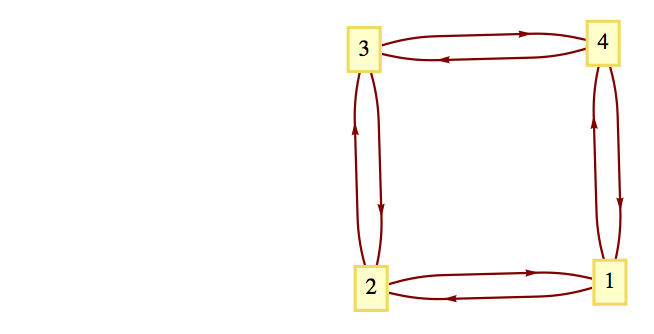
\includegraphics[width=0.7\linewidth]{images/fig-graph-12-5-2.png}
\caption*{\textbf{Figure 12.5.7:} Graph for exercise 4}
\end{figure}
\par\smallskip%
\noindent\textbf{Hint}.\quad%
\hypertarget{p-4693}{}%
The characteristic polynomial of the adjacency matrix is \(\lambda ^4 - 4 \lambda^2\).%
\end{divisionsolution}%
\begin{divisionsolution}{12.5.5.5}{}{exercise-12-5-5}%
\hypertarget{p-4694}{}%
Regarding Example~12.5.3,\leavevmode%
\begin{enumerate}[label=(\alph*)]
\item\hypertarget{li-2136}{}\hypertarget{p-4695}{}%
Use matrices to determine the number of paths of length 1 that exist from vertex \(a\) to each of the vertices in the given graph. Verify using the graph. Do the same for vertices \(b\) and \(c\).%
\item\hypertarget{li-2137}{}\hypertarget{p-4696}{}%
Verify all the details provided in the example.%
\item\hypertarget{li-2138}{}\hypertarget{p-4697}{}%
Use matrices to determine the number of paths of length 4 there between each pair of nodes in the graph. Verify your results using the graph.%
\end{enumerate}
%
\par\smallskip%
\noindent\textbf{Answer}.\quad%
\hypertarget{p-4698}{}%
\leavevmode%
\begin{enumerate}[label=(\alph*)]
\item\hypertarget{li-2139}{}\hypertarget{p-4699}{}%
Since   \(A=A^1= \left(
\begin{array}{ccc}
1 & 1 & 0 \\
1 & 0 & 1 \\
0 & 1 & 1 \\
\end{array}
\right)\),  there are 0 paths of length 1 from: node c to node a, node b to node b, and node a to node c; and there is 1 path of length 1 for every other pair of nodes.%
\item\hypertarget{li-2140}{}\hypertarget{p-4700}{}%
The characteristic polynomial is \(\lvert A-c I\rvert  = \left|
\begin{array}{ccc}
1-c & 1 & 0 \\
1 & -c & 1 \\
0 & 1 & 1-c \\
\end{array}
\right| = -c^3+2 c^2+c-2\)%
\par
\hypertarget{p-4701}{}%
Solving the characteristic equation \(-c^3+2 c^2+c-2=0\) we find solutions 1, 2, and -1.%
\par
\hypertarget{p-4702}{}%
If \(c=1\), we find the associated eigenvector by finding a nonzero solution to \(\left(
\begin{array}{ccc}
0 & 1 & 0 \\
1 & -1 & 1 \\
0 & 1 & 0 \\
\end{array}
\right)\left(
\begin{array}{c}
x_1 \\
x_2 \\
x_3 \\
\end{array}
\right)=\left(
\begin{array}{c}
0 \\
0 \\
0 \\
\end{array}
\right)\) One of these, which will be the first column of \(P\), is \(\left(
\begin{array}{c}
1 \\
0 \\
-1 \\
\end{array}
\right)\)%
\par
\hypertarget{p-4703}{}%
If \(c=2\), the system \(\left(
\begin{array}{ccc}
-1 & 1 & 0 \\
1 & -2 & 1 \\
0 & 1 & -1 \\
\end{array}
\right)\left(
\begin{array}{c}
x_1 \\
x_2 \\
x_3 \\
\end{array}
\right)=\left(
\begin{array}{c}
0 \\
0 \\
0 \\
\end{array}
\right)\)  yields eigenvectors, including \(\left(
\begin{array}{c}
1 \\
1 \\
1 \\
\end{array}
\right)\), which will be the second column of \(P\).%
\par
\hypertarget{p-4704}{}%
If  \(c = -1\), then the system determining the eigenvectors is \(\left(
\begin{array}{ccc}
2 & 1 & 0 \\
1 & 1 & 1 \\
0 & 1 & 2 \\
\end{array}
\right)\left(
\begin{array}{c}
x_1 \\
x_2 \\
x_3 \\
\end{array}
\right)=\left(
\begin{array}{c}
0 \\
0 \\
0 \\
\end{array}
\right)\) and we can select \(\left(
\begin{array}{c}
1 \\
-2 \\
1 \\
\end{array}
\right)\),  although any nonzero multiple of this vector could be the third column of \(P\).%
\item\hypertarget{li-2141}{}\hypertarget{p-4705}{}%
Assembling the results of part (b) we have \(P=\left(
\begin{array}{ccc}
1 & 1 & 1 \\
0 & 1 & -2 \\
-1 & 1 & 1 \\
\end{array}
\right)\) .%
\par
\hypertarget{p-4706}{}%
%
\begin{equation*}
\begin{split}
A^4  & = P \left(
\begin{array}{ccc}
1^4 & 0 & 0 \\
0 & 2^4 & 0 \\
0 & 0 & (-1)^{4 } \\
\end{array}
\right)P^{-1}= P \left(
\begin{array}{ccc}
1 & 0 & 0 \\
0 & 16 & 0 \\
0 & 0 & 1 \\
\end{array}
\right)P^{-1}\\
&=\left(
\begin{array}{ccc}
1 & 16 & 1 \\
0 & 16 & -2 \\
-1 & 16 & 1 \\
\end{array}
\right)\left(
\begin{array}{ccc}
\frac{1}{2} & 0 & -\frac{1}{2} \\
\frac{1}{3} & \frac{1}{3} & \frac{1}{3} \\
\frac{1}{6} & -\frac{1}{3} & \frac{1}{6} \\
\end{array}
\right)\\
&=\left(
\begin{array}{ccc}
6 & 5 & 5 \\
5 & 6 & 5 \\
5 & 5 & 6 \\
\end{array}
\right)\\
\end{split}
\end{equation*}
%
\par
\hypertarget{p-4707}{}%
Hence there are five different paths of length 4 between distinct vertices, and six different paths that start and end at the same vertex.  The reader can verify these facts from Figure~12.5.4%
\end{enumerate}
%
\end{divisionsolution}%
\begin{divisionsolution}{12.5.5.6}{}{exercise-524}%
\hypertarget{p-4708}{}%
Let \(A =\left(
\begin{array}{cc}
2 & -1 \\
-1 & 2 \\
\end{array}
\right)\)\leavevmode%
\begin{enumerate}[label=(\alph*)]
\item\hypertarget{li-2142}{}\hypertarget{p-4709}{}%
Find \(e^A\)%
\item\hypertarget{li-2143}{}\hypertarget{p-4710}{}%
Recall that \(\sin  x = \sum _{k=0}^{\infty } \frac{(-1)^k x^k}{(2 k+1)!}\)  and compute \(\sin  A\).%
\item\hypertarget{li-2144}{}\hypertarget{p-4711}{}%
Formulate a reasonable definition of the natural logarithm of a matrix and compute \(\ln  A\).%
\end{enumerate}
%
\end{divisionsolution}%
\begin{divisionsolution}{12.5.5.7}{}{exercise-525}%
\hypertarget{p-4712}{}%
We noted in Chapter 5 that since matrix algebra is not commutative under multiplication, certain difficulties arise.  Let \(A=\left(
\begin{array}{cc}
1 & 1 \\
0 & 0 \\
\end{array}
\right)\) and \(B=\left(
\begin{array}{cc}
0 & 0 \\
0 & 2 \\
\end{array}
\right)\).\leavevmode%
\begin{enumerate}[label=(\alph*)]
\item\hypertarget{li-2145}{}\hypertarget{p-4713}{}%
Compute   \(e^A\), \(e^B\), and \(e^{A+B}\).   Compare \(e^A e^{B}\), \(e^B e^A\) and \(e^{A+B}\) .%
\item\hypertarget{li-2146}{}\hypertarget{p-4714}{}%
Show that if \(\pmb{0}\) is the \(2\times 2\) zero matrix, then \(e^{\pmb{0}}= I\).%
\item\hypertarget{li-2147}{}\hypertarget{p-4715}{}%
Prove that if \(A\) and \(B\) are two matrices that do commute, then  \(e^{A+B}=e^Ae^B\), thereby proving that \(e^A\) and \(e^B\) commute.%
\item\hypertarget{li-2148}{}\hypertarget{p-4716}{}%
Prove that for any matrix \(A\),  \(\left(e^A\right)^{-1}= e^{-A}\).%
\end{enumerate}
%
\par\smallskip%
\noindent\textbf{Answer}.\quad%
\hypertarget{p-4717}{}%
\leavevmode%
\begin{enumerate}[label=(\alph*)]
\item\hypertarget{li-2149}{}\hypertarget{p-4718}{}%
\(e^A=\left(
\begin{array}{cc}
e & e \\
0 & 0 \\
\end{array}
\right)\) ,  \(e^B=\left(
\begin{array}{cc}
0 & 0 \\
0 & e^2 \\
\end{array}
\right)\),  and  \(e^{A+B}=\left(
\begin{array}{cc}
e & e^2-e \\
0 & e^2 \\
\end{array}
\right)\)%
\item\hypertarget{li-2150}{}\hypertarget{p-4719}{}%
Let \textbackslash{}pmb\textbraceleft{} 0\textbraceright{} be the zero matrix, \(e^{\pmb{0}}=I + \pmb{0}+\frac{\pmb{0}^2}{2}+\frac{\pmb{0}^3}{6}+\ldots =I\) .%
\item\hypertarget{li-2151}{}\hypertarget{p-4720}{}%
Assume that \(A\) and \(B\) commute. We will examine the first few terms in the product \(e^A e^B\). The pattern that is established does continue in general. In what follows, it is important that \(A B = B A\). For example, in the last step,   \((A+B)^2\) expands to \(A^2+A
B + B A + B^2\), not \(A^2+ 2 A B + B^2\),  if we can't assume commutativity.%
\begin{equation*}
\begin{split}
e^Ae^B &= \left(\sum _{k=0}^{\infty } \frac{A^k}{k!}\right) \left(\sum _{k=0}^{\infty } \frac{B^k}{k!}\right)\\
& =\left(I + A+\frac{A^2}{2}+ \frac{A^3}{6}+ \cdots \right)\left(I +B+\frac{B^2}{2}+ \frac{B^3}{6}+ \cdots \right)\\
&= I + A + B+ \frac{A^2}{2}+ A B + \frac{B^2}{2}+\frac{A^3}{6}+ \frac{A^2B}{2}+\frac{A B^2}{2}+ \frac{B^3}{6}+\cdots \\
&= I + (A+B) + \frac{1}{2}\left(A^2+ 2 A B + B^2\right)+ \frac{1}{6}\left(A^3+ 3A^2B+ 3A B^2+ B^3\right)+\cdots \\
&=I + (A+B)+ \frac{1}{2}(A+B)^2+ \frac{1}{6}(A+B)^3+\cdots \\
& =e^{A+B}\\
\end{split}
\end{equation*}
%
\item\hypertarget{li-2152}{}\hypertarget{p-4721}{}%
Since \(A\) and \(-A\) commute, we can apply part d;%
\begin{equation*}
e^Ae^{-A} = e^{A+(-A)} =e^{\pmb{0}} =I
\end{equation*}
%
\end{enumerate}
%
\end{divisionsolution}%
\begin{divisionsolution}{12.5.5.8}{}{exercise-526}%
\hypertarget{p-4722}{}%
Another observation for adjacency matrices: For the matrix in Example~12.5.3, note that the sum of the elements in the row corresponding to the node \(a\) (that is, the first row) gives the outdegree of \(a\). Similarly, the sum of the elements in any given column gives the indegree of the node corresponding to that column.%
\begin{figure}
\centering
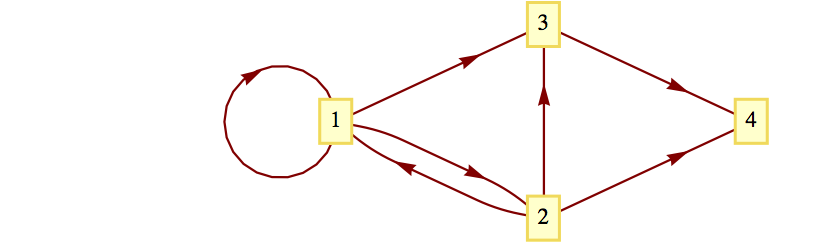
\includegraphics[width=0.7\linewidth]{images/fig-graph-12-5-3.png}
\caption*{\textbf{Figure 12.5.8:} Graph for exercise 8}
\end{figure}
\hypertarget{p-4723}{}%
\leavevmode%
\begin{enumerate}[label=(\alph*)]
\item\hypertarget{li-2153}{}\hypertarget{p-4724}{}%
Using the matrix \(A\) of Example~12.5.3, find the outdegree and the indegree of each node. Verify by the graph.%
\item\hypertarget{li-2154}{}\hypertarget{p-4725}{}%
Repeat part (a) for the directed graphs in Figure~12.5.8.%
\end{enumerate}
%
\end{divisionsolution}%
\section*{12.6 Linear Equations over the Integers Mod 2}
\addcontentsline{toc}{section}{12.6 Linear Equations over the Integers Mod 2}
\sectionmark{12.6 Linear Equations over the Integers Mod 2}
\subsection*{12.6.2 Exercises for this section}
\addcontentsline{toc}{subsection}{12.6.2 Exercises for this section}
\begin{divisionsolution}{12.6.2.1}{}{exercise-12-6-1}%
\hypertarget{p-4734}{}%
Solve the following systems, describing the solution sets completely:\leavevmode%
\begin{multicols}{2}
\begin{enumerate}[label=(\alph*)]
\item\hypertarget{li-2155}{}\hypertarget{p-4735}{}%
\(\begin{array}{r@{}r@{}r@{}r@{}r@{}r@{}}
x_1  & {}+{} & x_2 &       &     & = 0 \\
x_1  &       &     & {}+{} & x_3 & = 0 \\
\end{array} \)%
\item\hypertarget{li-2156}{}\hypertarget{p-4736}{}%
\(\begin{array}{r@{}r@{}r@{}r@{}r@{}r@{}r@{}r@{}}
x_1  & {}+{} & x_2 &       &    &       &        & = 0 \\
&       & x_2 & {}+{} & x_3&       &       &   = 0\\
&       &     &       & x_3& {}+{} & x_4   & = 1 \\
x_1  & {}+{} & x_2 & {}+{} & x_3&       &        &  = 1 \\
\end{array} \)%
\end{enumerate}
\end{multicols}
%
\par\smallskip%
\noindent\textbf{Answer}.\quad%
\hypertarget{p-4737}{}%
\leavevmode%
\begin{enumerate}[label=(\alph*)]
\item\hypertarget{li-2157}{}\hypertarget{p-4738}{}%
\(\{(0,0,0),(1,1,1)\}\)%
\item\hypertarget{li-2158}{}\hypertarget{p-4739}{}%
\(\{(1,1,1,0)\}\)%
\end{enumerate}
%
\end{divisionsolution}%
\begin{divisionsolution}{12.6.2.2}{}{exercise-12-6-3}%
\hypertarget{p-4740}{}%
This exercise provides an example in which the number of basic variables is less than the number of equations. The only difference between the two systems below is the right hand sides.  You can start with an augmented matrix having two right side columns and do row reduction for both systems at the same time.\leavevmode%
\begin{multicols}{2}
\begin{enumerate}[label=(\alph*)]
\item\hypertarget{li-2159}{}\hypertarget{p-4741}{}%
\(\begin{array}{r@{}r@{}r@{}r@{}r@{}r@{}r@{}r@{}}
x_1 & {}+{} &x_2 &       &    &{}+{} & x_4   &= 1 \\
x_1 &       &    & {}+{} &x_3 & {}+{} & x_4  &= 0 \\
&       & x_2 & {}+{} &x_3 &      &      &= 1 \\
\end{array}\)%
\item\hypertarget{li-2160}{}\hypertarget{p-4742}{}%
\(\begin{array}{r@{}r@{}r@{}r@{}r@{}r@{}r@{}r@{}}
x_1 & {}+{} &x_2 &       &    &{}+{} & x_4   &= 1 \\
x_1 &       &    & {}+{} &x_3 & {}+{} & x_4  &= 0 \\
&       & x_2 & {}+{} &x_3 &      &      &= 0 \\
\end{array}\)%
\end{enumerate}
\end{multicols}
%
\par\smallskip%
\noindent\textbf{Answer}.\quad%
\hypertarget{p-4743}{}%
As suggested here is the augmented matrix with both right sides, and its row reduction:%
\begin{equation*}
\begin{split}
\left(
\begin{array}{cccc|cc}
1 & 1 & 0 &  1 & 1 & 1 \\
1 & 0 & 1 &  1 & 0 & 0  \\
0 & 1 & 1 &  0 & 1 & 0  \\
\end{array}
\right) & \text{  }\longrightarrow \text{   }
\left(
\begin{array}{cccc|cc}
\textbf{1} & 0  & 1 &  1 & 0 & 0 \\
0 & \textbf{1}  & 1 &  0 & 1 & 0  \\
0 & 0                & 0 &  0 & 0 & 1  \\
\end{array}
\right)\\
\end{split}
\end{equation*}
There are only two basic variables here because the left side of the last equation is the sum of the  left sides of the first two equations.\leavevmode%
\begin{enumerate}[label=(\alph*)]
\item\hypertarget{li-2161}{}\hypertarget{p-4744}{}%
Ignoring the last column of both matrices, we see that the last equation of the first system reduces to \(0=0\), which is always true, and the first two equations yield two free variables, \(x_3\) and \(x_4\).  The general solution is the set of quadruples \(\{(x_3 +_2 x_4,x_3 +_2 1, x_3, x_4) \mid x_3, x_4 \in \mathbb{Z}_2 \}\).  The cardinality of the solution set is 4.%
\item\hypertarget{li-2162}{}\hypertarget{p-4745}{}%
If we replace the fifth column with the sixth one, the last row indicates that \(0=1\), which means that the solution set is empty.%
\end{enumerate}
%
\end{divisionsolution}%
\begin{divisionsolution}{12.6.2.3}{}{exercise-12-6-2}%
\hypertarget{p-4746}{}%
This exercise motivates the concept of a coset in Chapter 15.\leavevmode%
\begin{enumerate}[label=(\alph*)]
\item\hypertarget{li-2163}{}\hypertarget{p-4747}{}%
Solve the following system and prove that the solution set is a linear combination of vectors in \(\mathbb{Z}_{2}^{5}\)  and also a subgroup of the group \(\mathbb{Z}_{2}^{5}\) under coordinatewise mod 2 addition.%
\begin{equation*}
\begin{array}{r@{}r@{}r@{}r@{}r@{}r@{}r@{}r@{}r@{}r@{}}
x_1 & {}+{} &x_2 &       &    &     &     &{}+{} & x_5&= 0 \\
x_1 &       &    & {}+{} &x_3 &      &     &{}+{} & x_5&= 0 \\
x_1 &       &    & {}+{} &x_3 &{}+{} & x_4 &      &    &= 0 \\
&       & x_2   & {}+{} &x_3 &{}+{} & x_4 &      &    &= 0 \\
\end{array}
\end{equation*}
%
\item\hypertarget{li-2164}{}\hypertarget{p-4748}{}%
Describe the solution set to the following system as it relates to the solution set to the system in the previous part of this exercise.%
\begin{equation*}
\begin{array}{r@{}r@{}r@{}r@{}r@{}r@{}r@{}r@{}r@{}r@{}}
x_1 & {}+{} &x_2 &       &    &     &     &{}+{} & x_5&= 1 \\
x_1 &       &    & {}+{} &x_3 &      &     &{}+{} & x_5&= 0 \\
x_1 &       &    & {}+{} &x_3 &{}+{} & x_4 &      &    &= 1 \\
&       & x_2   & {}+{} &x_3 &{}+{} & x_4 &      &    &= 0 \\
\end{array}
\end{equation*}
%
\end{enumerate}
%
\par\smallskip%
\noindent\textbf{Answer}.\quad%
\hypertarget{p-4749}{}%
\leavevmode%
\begin{enumerate}[label=(\alph*)]
\item\hypertarget{li-2165}{}\hypertarget{p-4750}{}%
Row reduction produces a solution with one free variable, \(x_3\).%
\begin{equation*}
\begin{split}
(x_1, x_2, x_3, x_4, x_5)& =(x_3,x_3,x_3,0,0)\\
& = x_3 (1,1,1,0,0) \\
\end{split}
\end{equation*}
%
\par
\hypertarget{p-4751}{}%
The solution set has only two elements. It is \(\{(0,0,0,0,0), (1,1,1,0,0)\}\).  Since \(\mathbb{Z}_{2}^{5}\) is a finite group,  the solution set is a subgroup because it is closed with respect to coordinate-wise mod 2 addition.%
\item\hypertarget{li-2166}{}\hypertarget{p-4752}{}%
The row-reduced augmented matrix of coefficients provides the solution%
\begin{equation*}
\begin{split}
(x_1, x_2, x_3, x_4, x_5)& =(x_3,1+x_3,x_3,1,0)\\
& = (0,1,0,1,0) + x_3 (1,1,1,0,0) \\
\end{split}
\end{equation*}
%
\par
\hypertarget{p-4753}{}%
Therefore, the solution to this system is a shift of the solution set to the homogeneous system by the vector \((0,1,0,1,0)\), which is \(\{(0,1,0,1,0), (1,0,1,1,0)\}\)%
\end{enumerate}
%
\end{divisionsolution}%
\chapter*{13 Boolean Algebra}
\addcontentsline{toc}{chapter}{13 Boolean Algebra}
\chaptermark{13 Boolean Algebra}
\section*{13.1 Posets Revisited}
\addcontentsline{toc}{section}{13.1 Posets Revisited}
\sectionmark{13.1 Posets Revisited}
\subsection*{13.1 Exercises for Section 13.1}
\addcontentsline{toc}{subsection}{13.1 Exercises for Section 13.1}
\begin{divisionsolution}{13.1.1}{}{exercise-13-1-1}%
\hypertarget{p-4792}{}%
Consider the poset \((D_{30},\mid)\), where \(D_{30} = \{1,2, 3, 5, 6, 10, 15, 30\}\).\leavevmode%
\begin{enumerate}[label=(\alph*)]
\item\hypertarget{li-2184}{}\hypertarget{p-4793}{}%
Find all lower bounds of 10 and 15.%
\item\hypertarget{li-2185}{}\hypertarget{p-4794}{}%
Find the greatest lower bound  of 10 and 15.%
\item\hypertarget{li-2186}{}\hypertarget{p-4795}{}%
Find all upper bounds of 10 and 15.%
\item\hypertarget{li-2187}{}\hypertarget{p-4796}{}%
Determine the least upper bound  of 10 and 15.%
\item\hypertarget{li-2188}{}\hypertarget{p-4797}{}%
Draw the Hasse diagram for \(D_{30}\) with respect to \(\div\). Compare this Hasse diagram with that of Example~13.1.10. Note that the two diagrams are structurally the same.%
\end{enumerate}
%
\par\smallskip%
\noindent\textbf{Answer}.\quad%
\hypertarget{p-4798}{}%
\leavevmode%
\begin{multicols}{2}
\begin{enumerate}[label=(\alph*)]
\item\hypertarget{li-2189}{}\hypertarget{p-4799}{}%
1, 5%
\item\hypertarget{li-2190}{}\hypertarget{p-4800}{}%
5%
\item\hypertarget{li-2191}{}\hypertarget{p-4801}{}%
30%
\item\hypertarget{li-2192}{}\hypertarget{p-4802}{}%
30%
\item\hypertarget{li-2193}{}\hypertarget{p-4803}{}%
See the Sage cell below with the default input displaying a Hasse diagram for \(D_{12}\).%
\end{enumerate}
\end{multicols}
%
\begin{sageinput}
Posets.DivisorLattice(12).show()
\end{sageinput}
\begin{sageoutput}

\end{sageoutput}
\end{divisionsolution}%
\begin{divisionsolution}{13.1.2}{}{exercise-531}%
\hypertarget{p-4804}{}%
List the elements of the sets \(D_8\), \(D_{50}\), and \(D_{1001}\). For each set, draw the Hasse diagram for ``divides.''%
\end{divisionsolution}%
\begin{divisionsolution}{13.1.3}{}{exercise-13-1-3}%
\hypertarget{p-4805}{}%
Figure~13.1.12 contains Hasse diagrams of posets.\leavevmode%
\begin{enumerate}[label=(\alph*)]
\item\hypertarget{li-2194}{}\hypertarget{p-4806}{}%
Determine the least upper bound  and greatest lower bound  of all pairs of elements when they exist. Indicate those pairs that do not have a least upper bound  (or a greatest lower bound ).%
\item\hypertarget{li-2195}{}\hypertarget{p-4807}{}%
Find the least and greatest elements when they exist.%
\end{enumerate}
%
\begin{figure}
\centering
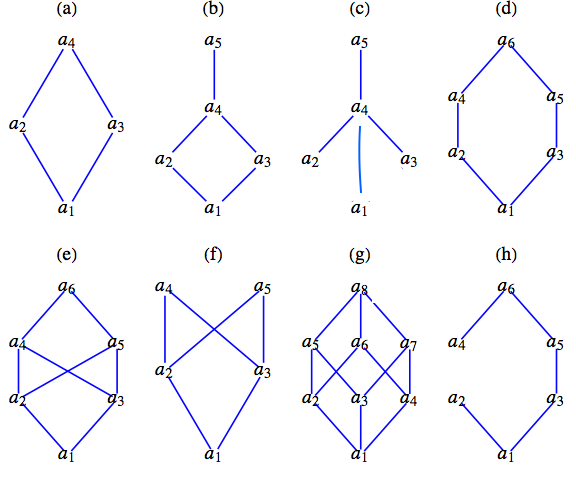
\includegraphics[width=0.8\linewidth]{images/fig-exercise-13-1-3.png}
\caption*{\textbf{Figure 13.1.12:} Figure for Exercise 3}
\end{figure}
\par\smallskip%
\noindent\textbf{Answer}.\quad%
\hypertarget{p-4808}{}%
\leavevmode%
\begin{itemize}[label=\textbullet]
\item{}\hypertarget{p-4809}{}%
Solution for Hasse diagram (b):%
\begin{itemize}[label=$\circ$]
\item{}\hypertarget{p-4810}{}%
%
\begin{equation*}
\begin{array}{c|c}
\begin{array}{c|ccccc}
\lor &a_1 & a_2 & a_3 & a_4 & a_5 \\
\hline
a_1 & a_1 &a_2 & a_3 & a_4 & a_5 \\
a_2 & a_2 & a_2 & a_4 & a_4 & a_5 \\
a_3 &a_3 & a_4 & a_3 & a_4 & a_5 \\
a_4 & a_4 & a_4 & a_4 & a_4 & a_5 \\
a_5 & a_5 & a_5 & a_5 & a_5 & a_5 \\
\end{array}
&\quad
\begin{array}{c|ccccc}
\land & a_1 & a_2 & a_3 & a_4 & a_5 \\\hline
a_1 &	 a_1 & a_1 & a_1 & a_1 & a_1 \\
a_2 &	a_1 & a_2 & a_1 & a_2 & a_2 \\
a_3 &	a_1 & a_1 & a_3 & a_3 & a_3 \\
a_4 &	a_1 & a_2 & a_3 & a_4 & a_4 \\
a_5 &	a_1 & a_2 & a_3 & a_4 & a_5 \\
\end{array}
\end{array}
\end{equation*}
%
\par
\hypertarget{p-4811}{}%
\(a_1\) is the least element and \(a_5\) is the greatest element.%
\end{itemize}
%
\item{}\hypertarget{p-4812}{}%
Partial solution for Hasse diagram (f):%
\begin{itemize}[label=$\circ$]
\item{}\hypertarget{p-4813}{}%
\(\textrm{ lub}\left(a_2, a_3\right)\) and \(\textrm{ lub}\left( a_4,a_5\right)\)  do not exist.%
\item{}\hypertarget{p-4814}{}%
No greatest element exists, but \(a_1\) is the least element.%
\end{itemize}
%
\end{itemize}
%
\end{divisionsolution}%
\begin{divisionsolution}{13.1.4}{}{exercise-533}%
\hypertarget{p-4815}{}%
For the poset \((\mathbb{N},\leq )\), what are the greatest lower bound and least upper bound of two elements \(a\) and \(b\)? Are there least and\slash{}or greatest elements?%
\end{divisionsolution}%
\begin{divisionsolution}{13.1.5}{}{exercise-534}%
\hypertarget{p-4816}{}%
\leavevmode%
\begin{enumerate}[label=(\alph*)]
\item\hypertarget{li-2201}{}\hypertarget{p-4817}{}%
Prove the second part of Theorem~13.1.6, the least upper bound of two elements in a poset is unique, it one exists.%
\item\hypertarget{li-2202}{}\hypertarget{p-4818}{}%
Prove that if a poset \(L\) has a least element, then that element is unique.%
\end{enumerate}
%
\par\smallskip%
\noindent\textbf{Answer}.\quad%
\hypertarget{p-4819}{}%
If \(0\) and \(0'\) are distinct least elements, then%
\begin{equation*}
\left.
\begin{array}{cc}
0\leq 0' & \textrm{ since } 0 \textrm{ is a least element} \\
0'\leq 0 & \textrm{ since } 0' \textrm{ is a least element} \\
\end{array}
\right\}\Rightarrow  0=0' \textrm{ by antisymmetry, a contradiction}
\end{equation*}
%
\end{divisionsolution}%
\begin{divisionsolution}{13.1.6}{}{exercise-535}%
\hypertarget{p-4820}{}%
We naturally order the numbers in \(A_m = \{1, 2, . . . , m\}\) with ``less than or equal to,'' which is a partial ordering. We define an ordering, \(\preceq\)  on the elements of \(A_m \times  A_n\) by%
\begin{equation*}
(a, b) \preceq  (a', b') \Leftrightarrow a \leq  a' \textrm{ and } b \leq  b'
\end{equation*}
\leavevmode%
\begin{enumerate}[label=(\alph*)]
\item\hypertarget{li-2203}{}\hypertarget{p-4821}{}%
Prove that \(\preceq\) is a partial ordering on \(A_m \times  A_n\).%
\item\hypertarget{li-2204}{}\hypertarget{p-4822}{}%
Draw the ordering diagrams for \(\preceq\) on \(A_2 \times  A_2\), \(A_2\times  A_3\), and \(A_3 \times  A_3\).%
\item\hypertarget{li-2205}{}\hypertarget{p-4823}{}%
In general, how does one determine the least upper bound  and greatest lower bound of two elements of \(A_m \times  A_n\), \((a, b)\) and \((a',b')\)?%
\item\hypertarget{li-2206}{}\hypertarget{p-4824}{}%
Are there least and\slash{}or greatest elements in \(A_m \times  A_n\)?%
\end{enumerate}
%
\end{divisionsolution}%
\section*{13.2 Lattices}
\addcontentsline{toc}{section}{13.2 Lattices}
\sectionmark{13.2 Lattices}
\subsection*{13.2 Exercises for Section 13.2}
\addcontentsline{toc}{subsection}{13.2 Exercises for Section 13.2}
\begin{divisionsolution}{13.2.1}{}{exercise-536}%
\hypertarget{p-4839}{}%
Let \(L\) be the set of all propositions generated by \(p\) and \(q\).  What are the meet and join operations in this lattice under implication?   What are the maximum and minimum elements?%
\end{divisionsolution}%
\begin{divisionsolution}{13.2.2}{}{exercise-537}%
\hypertarget{p-4840}{}%
Which of the posets in Exercise~13.1.3 are lattices? Which of the lattices are distributive?%
\end{divisionsolution}%
\begin{divisionsolution}{13.2.3}{}{exercise-538}%
\hypertarget{p-4841}{}%
\leavevmode%
\begin{enumerate}[label=(\alph*)]
\item\hypertarget{li-2209}{}\hypertarget{p-4842}{}%
State the commutative laws, associative laws, idempotent laws, and absorption laws for lattices.%
\item\hypertarget{li-2210}{}\hypertarget{p-4843}{}%
Prove laws you stated.%
\end{enumerate}
%
\end{divisionsolution}%
\begin{divisionsolution}{13.2.4}{}{exercise-539}%
\hypertarget{p-4844}{}%
Demonstrate that the pentagon lattice is nondistributive.%
\end{divisionsolution}%
\begin{divisionsolution}{13.2.5}{}{exercise-540}%
\hypertarget{p-4845}{}%
What is a reasonable definition of the term \terminology{sublattice}?%
\par\smallskip%
\noindent\textbf{Answer}.\quad%
\hypertarget{p-4846}{}%
One reasonable definition would by this:  Let \([L; \lor, \land ]\) be a lattice and let \(K\) be a nonempty subset of \(L\).  Then \(K\) is a sublattice of \(L\) if and only if \(K\) is closed under both \(\lor\) and \(\land\)%
\end{divisionsolution}%
\begin{divisionsolution}{13.2.6}{}{exercise-541}%
\hypertarget{p-4847}{}%
Let \([L; \lor  , \land ]\) be a lattice based on a partial ordering \(\preceq\).   Prove that if \(a, b, c \in L\),\leavevmode%
\begin{enumerate}[label=(\alph*)]
\item\hypertarget{li-2211}{}\hypertarget{p-4848}{}%
\(a \preceq a \lor  b \).%
\item\hypertarget{li-2212}{}\hypertarget{p-4849}{}%
\(a \land  b \preceq  a\).%
\item\hypertarget{li-2213}{}\hypertarget{p-4850}{}%
\(b \preceq  a\) and \(c \preceq  a \Rightarrow   b \lor  c \preceq a\).%
\end{enumerate}
%
\end{divisionsolution}%
\section*{13.3 Boolean Algebras}
\addcontentsline{toc}{section}{13.3 Boolean Algebras}
\sectionmark{13.3 Boolean Algebras}
\subsection*{13.3 Exercises for Section 13.3}
\addcontentsline{toc}{subsection}{13.3 Exercises for Section 13.3}
\begin{divisionsolution}{13.3.1}{}{exercise-542}%
\hypertarget{p-4872}{}%
Determine the complement of each element \(B \in  L\) in Example~13.3.4. Is this lattice a Boolean algebra? Why?%
\par\smallskip%
\noindent\textbf{Answer}.\quad%
\hypertarget{p-4873}{}%
\(\begin{array}{cc}
B & \textrm{ Complement of } B \\
\hline 
\begin{array}{c}
\emptyset  \\
\{a\} \\
\{b\} \\
\{c\} \\
\{a,b\} \\
\{a,c\} \\
\{b,c\} \\
A \\
\end{array}
& 
\begin{array}{c}
A \\
\{b,c\} \\
\{a,c\} \\
\{a,b\} \\
\{c\} \\
\{b\} \\
\{a\} \\
\emptyset  \\
\end{array}
\\
\end{array}\)%
\par
\hypertarget{p-4874}{}%
This lattice is a Boolean algebra since it is a distributive complemented lattice.%
\end{divisionsolution}%
\begin{divisionsolution}{13.3.2}{}{exercise-543}%
\hypertarget{p-4875}{}%
\leavevmode%
\begin{enumerate}[label=(\alph*)]
\item\hypertarget{li-2214}{}\hypertarget{p-4876}{}%
Determine the complement of each element of \(D_6\) in \(\left[D_6; \lor , \land \right]\).%
\item\hypertarget{li-2215}{}\hypertarget{p-4877}{}%
Repeat part a using the lattice in Example~13.2.5.%
\item\hypertarget{li-2216}{}\hypertarget{p-4878}{}%
Repeat part a using the lattice in Exercise~13.1.1.%
\item\hypertarget{li-2217}{}\hypertarget{p-4879}{}%
Are the lattices in parts a, b, and c Boolean algebras? Why?%
\end{enumerate}
%
\end{divisionsolution}%
\begin{divisionsolution}{13.3.3}{}{exercise-544}%
\hypertarget{p-4880}{}%
Determine which of the lattices of Exercise~13.1.3 of Section 13.1 are Boolean algebras.%
\par\smallskip%
\noindent\textbf{Answer}.\quad%
\hypertarget{p-4881}{}%
a and g.%
\end{divisionsolution}%
\begin{divisionsolution}{13.3.4}{}{exercise-545}%
\hypertarget{p-4882}{}%
Let \(A = \{a, b\}\) and \(B = \mathcal{P}(A)\).\leavevmode%
\begin{enumerate}[label=(\alph*)]
\item\hypertarget{li-2218}{}\hypertarget{p-4883}{}%
Prove that \([B; \cup, \cap, \hspace{1 mm}^c ]\) is a Boolean algebra.%
\item\hypertarget{li-2219}{}\hypertarget{p-4884}{}%
Write out the operation tables for the Boolean algebra.%
\end{enumerate}
%
\end{divisionsolution}%
\begin{divisionsolution}{13.3.5}{}{exercise-546}%
\hypertarget{p-4885}{}%
It can be shown that the following statement, \(S\), holds for any Boolean algebra \([B; \lor , \land, -]\) : \((a \land  b) = a\) if and only if \(a \leq  b\).\leavevmode%
\begin{enumerate}[label=(\alph*)]
\item\hypertarget{li-2220}{}\hypertarget{p-4886}{}%
Write the dual, \(S^*\), of the statement \(S\).%
\item\hypertarget{li-2221}{}\hypertarget{p-4887}{}%
Write the statement \(S\) and its dual, \(S^*\), in the language of sets.%
\item\hypertarget{li-2222}{}\hypertarget{p-4888}{}%
Are the statements in part b true for all sets?%
\item\hypertarget{li-2223}{}\hypertarget{p-4889}{}%
Write the statement \(S\) and its dual, \(S^*\), in the language of logic.%
\item\hypertarget{li-2224}{}\hypertarget{p-4890}{}%
Are the statements in part d true for all propositions?%
\end{enumerate}
%
\par\smallskip%
\noindent\textbf{Answer}.\quad%
\hypertarget{p-4891}{}%
\leavevmode%
\begin{enumerate}[label=(\alph*)]
\item\hypertarget{li-2225}{}\hypertarget{p-4892}{}%
\(S^*:a \lor  b= a \textrm{ if } a \geq  b\)%
\item\hypertarget{li-2226}{}\hypertarget{p-4893}{}%
The dual of  \(S:A\cap B = A\textrm{ if }A \subseteq B\) is \(S^*:A \cup B = A\textrm{ if } A \supseteq B\)%
\item\hypertarget{li-2227}{}\hypertarget{p-4894}{}%
Yes%
\item\hypertarget{li-2228}{}\hypertarget{p-4895}{}%
The dual of \(S:p \land q\Leftrightarrow p\textrm{    }\textrm{ if } p\Rightarrow q\) is \(S^*:p \lor q\Leftrightarrow p \textrm{ if } q\Rightarrow p\)%
\item\hypertarget{li-2229}{}\hypertarget{p-4896}{}%
Yes%
\end{enumerate}
%
\end{divisionsolution}%
\begin{divisionsolution}{13.3.6}{}{exercise-547}%
\hypertarget{p-4897}{}%
State the dual of:\leavevmode%
\begin{enumerate}[label=(\alph*)]
\item\hypertarget{li-2230}{}\hypertarget{p-4898}{}%
\(a \lor  (b \land  a) = a\).%
\item\hypertarget{li-2231}{}\hypertarget{p-4899}{}%
\(a \lor  \left(\overline{\left(\bar{b} \lor  a\right) \land  b}\right) = 1\).%
\item\hypertarget{li-2232}{}\hypertarget{p-4900}{}%
\(\left(\overline{a \land  \bar{b}}\right) \land  b = a\lor  b\).%
\end{enumerate}
%
\end{divisionsolution}%
\begin{divisionsolution}{13.3.7}{}{exercise-548}%
\hypertarget{p-4901}{}%
Formulate a definition for isomorphic Boolean algebras.%
\par\smallskip%
\noindent\textbf{Answer}.\quad%
\hypertarget{p-4902}{}%
\([B; \land, \lor, -]\) is isomorphic to \([B';\land, \lor, \tilde{}]\) if and only if there exists a  function \(T:B \to  B'\) such that\leavevmode%
\begin{enumerate}[label=(\alph*)]
\item\hypertarget{li-2233}{}\hypertarget{p-4903}{}%
\(T\) is a bijection;%
\item\hypertarget{li-2234}{}\hypertarget{p-4904}{}%
\(T(a\land b)=T(a)\land T(b)\quad \textrm{ for} \textrm{ all } a,b\in B\)%
\item\hypertarget{li-2235}{}\hypertarget{p-4905}{}%
\(T(a\lor b)=T(a)\lor T(b)\quad \textrm{ for} \textrm{ all } a, b \in B\)%
\item\hypertarget{li-2236}{}\hypertarget{p-4906}{}%
\(T(\bar{a})=\tilde{T(a)}\quad \textrm{ for all } a\in B\).%
\end{enumerate}
%
\end{divisionsolution}%
\begin{divisionsolution}{13.3.8}{}{exercise-549}%
\hypertarget{p-4907}{}%
For what positive integers, \(n\), does the lattice \([D_n,\mid]\) produce a boolean algebra?%
\end{divisionsolution}%
\section*{13.4 Atoms of a Boolean Algebra}
\addcontentsline{toc}{section}{13.4 Atoms of a Boolean Algebra}
\sectionmark{13.4 Atoms of a Boolean Algebra}
\subsection*{13.4 Exercises for Section 13.4}
\addcontentsline{toc}{subsection}{13.4 Exercises for Section 13.4}
\begin{divisionsolution}{13.4.1}{}{exercise-550}%
\hypertarget{p-4932}{}%
\leavevmode%
\begin{enumerate}[label=(\alph*)]
\item\hypertarget{li-2240}{}\hypertarget{p-4933}{}%
Show that \(a = 2\) is an atom of the Boolean algebra \(\left[D_{30}; \lor , \land, - \right]\).%
\item\hypertarget{li-2241}{}\hypertarget{p-4934}{}%
Repeat part a for the elements 3 and 5 of \(D_{30}\).%
\item\hypertarget{li-2242}{}\hypertarget{p-4935}{}%
Verify Theorem Theorem~13.4.5 for the Boolean algebra \(\left[D_{30}; \lor , \land, - \right]\).%
\end{enumerate}
%
\par\smallskip%
\noindent\textbf{Answer}.\quad%
\hypertarget{p-4936}{}%
\leavevmode%
\begin{enumerate}[label=(\alph*)]
\item\hypertarget{li-2243}{}\hypertarget{p-4937}{}%
For \(a = 3\) we must show that for each \(x \in  D_{30}\)  one of the following is true: \(x\land 3=3\) or \(x\land 3=1\).  We do this through the following table:%
\begin{equation*}
\begin{array}{cc}
x & \textrm{ verification} \\
\hline
\begin{array}{c}
1 \\
2 \\
3 \\
5 \\
6 \\
10 \\
15 \\
30 \\
\end{array}
& 
\begin{array}{c}
1\land 3=1 \\
2\land 3=1 \\
3\land 3=3 \\
5\land 3=1 \\
6\land 3=3 \\
20\land 3=1 \\
15\land 3=3 \\
30\land 3=3 \\
\end{array}
\\
\end{array}
\end{equation*}
For \(a=5\), a similar verification can be performed.%
\item\hypertarget{li-2244}{}\hypertarget{p-4938}{}%
\(6 = 2 \lor  3\), \(10 = 2 \lor  5\), \(15 = 3 \lor  5\), and \(30 = 2 \lor  3 \lor  5\).%
\end{enumerate}
%
\end{divisionsolution}%
\begin{divisionsolution}{13.4.2}{}{exercise-551}%
\hypertarget{p-4939}{}%
Let \(A = \{a, b, c\}\).\leavevmode%
\begin{enumerate}[label=(\alph*)]
\item\hypertarget{li-2245}{}\hypertarget{p-4940}{}%
Rewrite the definition of atom for \([\mathcal{P}(A); \cup , \cap, c ]\). What does \(a \leq  x\) mean in this example?%
\item\hypertarget{li-2246}{}\hypertarget{p-4941}{}%
Find all atoms of \([\mathcal{P}(A); \cup , \cap, c ]\).%
\item\hypertarget{li-2247}{}\hypertarget{p-4942}{}%
Verify Theorem~13.4.5 for \([\mathcal{P}(A); c, \cup , \cap ]\).%
\end{enumerate}
%
\end{divisionsolution}%
\begin{divisionsolution}{13.4.3}{}{exercise-552}%
\hypertarget{p-4943}{}%
Verify Theorem~13.4.6 and its corollaries for the Boolean algebras in Exercises 1 and 2 of this section.%
\par\smallskip%
\noindent\textbf{Answer}.\quad%
\hypertarget{p-4944}{}%
If \(B = D_{30}\textrm{ }\) 30 then \(A = \{2, 3, 5\}\) and \(D_{30}\) is isomorphic to \(\mathcal{P}(A)\), where \(\begin{array}{cc}
1\leftrightarrow \emptyset \textrm{     } & 5\leftrightarrow  \{5\} \\
2\leftrightarrow  \{2\}\textrm{     } & 10\leftrightarrow  \{2,5\} \\
3\leftrightarrow  \{3\}\textrm{     } & 15\leftrightarrow  \{3,5\} \\
6\leftrightarrow  \{2,3\}\textrm{     } & 30\leftrightarrow  \{2,3,5\} \\
\end{array}\)   and   \(\begin{array}{c}
\textrm{ Join} \leftrightarrow  \textrm{ Union} \\
\textrm{ Meet}\leftrightarrow  \textrm{ Intersection} \\
\textrm{ Complement}\leftrightarrow  \textrm{ Set} \textrm{ Complement}  \\
\end{array}\)%
\end{divisionsolution}%
\begin{divisionsolution}{13.4.4}{}{exercise-553}%
\hypertarget{p-4945}{}%
Give an example of a Boolean algebra of order 16 whose elements are certain subsets of the set \({1, 2, 3, 4, 5, 6, 7}\)%
\end{divisionsolution}%
\begin{divisionsolution}{13.4.5}{}{exercise-554}%
\hypertarget{p-4946}{}%
Corollary~13.4.7 implies that there do not exist Boolean algebras of orders 3, 5, 6, 7, 9, etc. (orders different from \(2^n\)). Without this corollary, directly show that we cannot have a Boolean algebra of order 3.%
\par\smallskip%
\noindent\textbf{Hint}.\quad%
\hypertarget{p-4947}{}%
Assume that \([B; \lor , \land, - ]\) is a Boolean algebra of order 3 where \(B = \{0,
x, 1\}\) and show that this cannot happen by investigating the possibilities for its operation tables.%
\par\smallskip%
\noindent\textbf{Answer}.\quad%
\hypertarget{p-4948}{}%
Assume that \(x \neq  0 \textrm{ or } 1\) is the third element of a Boolean algebra. Then there is only one possible set of tables for join and meet, all following from required properties of the Boolean algebra.%
\begin{equation*}
\begin{array}{lr}
\begin{array}{c|c}
\lor  & 
\begin{array}{ccc}
0 & x & 1 \\
\end{array}
\\
\hline
\begin{array}{c}
0 \\
x \\
1 \\
\end{array}
& 
\begin{array}{ccc}
0 & x & 1 \\
x & x & 1 \\
1 & 1 & 1 \\
\end{array}
\\
\end{array}       
& 
\begin{array}{c|c}
\land  & 
\begin{array}{ccc}
0 & x & 1 \\
\end{array}
\\
\hline
\begin{array}{c}
0 \\
x \\
1 \\
\end{array}
& 
\begin{array}{ccc}
0 & 0 & 0 \\
0 & x & x \\
0 & x & 1 \\
\end{array}
\\
\end{array}
\end{array}
\end{equation*}
Next, to find the complement of \(x\) we want \(y\) such that \(x \land  y = 0\) and \(x \lor  y = 1\). No element satisfies both conditions; hence the lattice is not complemented and cannot be a Boolean algebra. The lack of a complement can also be seen from the ordering diagram from which \(\land\) and \(\lor\) must be derived.%
\end{divisionsolution}%
\begin{divisionsolution}{13.4.6}{}{exercise-555}%
\hypertarget{p-4949}{}%
\leavevmode%
\begin{enumerate}[label=(\alph*)]
\item\hypertarget{li-2248}{}\hypertarget{p-4950}{}%
There are many different, yet isomorphic, Boolean algebras with two elements. Describe one such Boolean algebra that is derived from a power set, \(\mathcal{P}(A)\), under \(\subseteq\). Describe a second that is described from \(D_n\), for some \(n \in  P\), under ``divides.''%
\item\hypertarget{li-2249}{}\hypertarget{p-4951}{}%
Since the elements of a two-element Boolean algebra must be the greatest and least elements, 1 and 0, the tables for the operations on \(\{0, 1\}\) are determined by the Boolean algebra laws. Write out the operation tables for \([\{0, 1\}; \lor , \land, -]\).%
\end{enumerate}
%
\end{divisionsolution}%
\begin{divisionsolution}{13.4.7}{}{exercise-556}%
\hypertarget{p-4952}{}%
Find a Boolean algebra with a countably infinite number of elements.%
\par\smallskip%
\noindent\textbf{Answer}.\quad%
\hypertarget{p-4953}{}%
Let \(X\) be any countably infinite set, such as the integers. A subset of \(X\) is \terminology{cofinite} if it is finite or its complement is finite. The set of all cofinite subsets of \(X\) is:\leavevmode%
\begin{enumerate}[label=(\alph*)]
\item\hypertarget{li-2250}{}\hypertarget{p-4954}{}%
Countably infinite - this might not be obvious, but here is a hint.  Assume \(X=\left\{x_0,x_1,x_2,\ldots \right\}\).  For each finite subset \(A\) of \(X\),  map that set to the integer \(\sum _{i=0}^{\infty } \chi _A \left(x_i\right)2^i\) You can do a similar thing to sets that have a finite complement, but map them to negative integers.  Only one minor adjustment needs to be made to accommodate both the empty set and \(X\).%
\item\hypertarget{li-2251}{}\hypertarget{p-4955}{}%
Closed under union%
\item\hypertarget{li-2252}{}\hypertarget{p-4956}{}%
Closed under intersection, and%
\item\hypertarget{li-2253}{}\hypertarget{p-4957}{}%
Closed under complementation.%
\end{enumerate}
Therefore, if \(B =\{A \subseteq  X : A \textrm{ is cofinite}\}\), then \(B\) is a countable Boolean algebra under the usual set operations.%
\end{divisionsolution}%
\begin{divisionsolution}{13.4.8}{}{exercise-557}%
\hypertarget{p-4958}{}%
Prove that the direct product of two Boolean algebras is a Boolean algebra.%
\par\smallskip%
\noindent\textbf{Hint}.\quad%
\hypertarget{p-4959}{}%
``Copy'' the corresponding proof for groups in Section 11.6.%
\end{divisionsolution}%
\begin{divisionsolution}{13.4.9}{}{exercise-set-boolean-isomorphism}%
\hypertarget{p-4960}{}%
Prove if two finite sets \(A_1\) and \(A_2\) both have \(n\) elements then \([\mathcal{P}(A_1);  \cup , \cap, \hspace{1 mm}^c]\) is isomorphic to \([\mathcal{P}(A_2);  \cup , \cap, \hspace{1 mm}^c]\)%
\end{divisionsolution}%
\begin{divisionsolution}{13.4.10}{}{exercise-covering-definition}%
\hypertarget{p-4961}{}%
Prove an element of a Boolean algebra is an atom if and only if it covers the zero element.%
\end{divisionsolution}%
\section*{13.5 Finite Boolean Algebras as \(n\)-tuples of 0's and 1's}
\addcontentsline{toc}{section}{13.5 Finite Boolean Algebras as \(n\)-tuples of 0's and 1's}
\sectionmark{13.5 Finite Boolean Algebras as \(n\)-tuples of 0's and 1's}
\subsection*{13.5 Exercises for Section 13.5}
\addcontentsline{toc}{subsection}{13.5 Exercises for Section 13.5}
\begin{divisionsolution}{13.5.1}{}{exercise-560}%
\hypertarget{p-4967}{}%
\leavevmode%
\begin{enumerate}[label=(\alph*)]
\item\hypertarget{li-2254}{}\hypertarget{p-4968}{}%
Write out the operation tables for \(\left[B_2^2; \lor , \land, - \right].\)%
\item\hypertarget{li-2255}{}\hypertarget{p-4969}{}%
Draw the Hasse diagram for \(\left[B_2^2; \lor , \land, - \right]\) and compare your results with  Figure~6.3.6.%
\item\hypertarget{li-2256}{}\hypertarget{p-4970}{}%
Find the atoms of this Boolean algebra.%
\end{enumerate}
%
\par\smallskip%
\noindent\textbf{Answer}.\quad%
\hypertarget{p-4971}{}%
\leavevmode%
\begin{enumerate}[label=(\alph*)]
\item\hypertarget{li-2257}{}\hypertarget{p-4972}{}%
%
\begin{equation*}
\begin{array}{lc} 
\begin{array}{c|cccc}
\lor & (0,0) & (0,1) & (1,0) & (1,1) \\
\hline
(0,0) & (0,0) & (0,1) & (1,0) & (1,1) \\
(0,1) &(0,1) & (0,1) & (1,1) & (1,1) \\
(1,0) & (1,0) & (1,1) & (1,0) & (1,1) \\
(1,1) & (1,1) & (1,1) & (1,1) & (1,1) \\
\end{array}
&\\
\begin{array}{c|cccc}
\land & (0,0) & (0,1) & (1,0) & (1,1) \\
\hline
(0,0) &(0,0) & (0,0) & (0,0) & (0,0) \\
(0,1) &(0,0) & (0,1) & (0,0) & (0,1) \\
(1,0) &(0,0) & (0,0) & (1,0) & (1,0) \\
(1,1) &(0,0) & (0,1) & (1,0) & (1,1) \\
\end{array}
&
\begin{array}{c|c}
u & \overset{\pmb{\_}}{u} \\
\hline
(0,0) & (1,1) \\
(0,1) &(1,0) \\
(1,0) &(0,1) \\
(1,1) &(0,0) \\
\end{array}
\\
\end{array}
\end{equation*}
%
\item\hypertarget{li-2258}{}\hypertarget{p-4973}{}%
The graphs are isomorphic.%
\item\hypertarget{li-2259}{}\hypertarget{p-4974}{}%
(0, 1) and (1,0)%
\end{enumerate}
%
\end{divisionsolution}%
\begin{divisionsolution}{13.5.2}{}{exercise-561}%
\hypertarget{p-4975}{}%
\leavevmode%
\begin{enumerate}[label=(\alph*)]
\item\hypertarget{li-2260}{}\hypertarget{p-4976}{}%
Write out the operation tables for \(\left[B_2^3; \lor , \land, - \right].\)%
\item\hypertarget{li-2261}{}\hypertarget{p-4977}{}%
Draw the Hasse diagram for \(\left[B_2^3; \lor , \land , - \right]\)%
\end{enumerate}
%
\end{divisionsolution}%
\begin{divisionsolution}{13.5.3}{}{exercise-562}%
\hypertarget{p-4978}{}%
\leavevmode%
\begin{enumerate}[label=(\alph*)]
\item\hypertarget{li-2262}{}\hypertarget{p-4979}{}%
List all atoms of \(B_2^4\).%
\item\hypertarget{li-2263}{}\hypertarget{p-4980}{}%
Describe the atoms of \(B_2^n, n \geq 1\).%
\end{enumerate}
%
\par\smallskip%
\noindent\textbf{Answer}.\quad%
\hypertarget{p-4981}{}%
\leavevmode%
\begin{enumerate}[label=(\alph*)]
\item\hypertarget{li-2264}{}\hypertarget{p-4982}{}%
\((1, 0, 0, 0)\), \((0, 1, 0, 0)\), \((0, 0, 1, 0)\), and \((0, 0, 0, 1)\) are the atoms.%
\item\hypertarget{li-2265}{}\hypertarget{p-4983}{}%
The \(n\)-tuples of bits with exactly one 1.%
\end{enumerate}
%
\end{divisionsolution}%
\begin{divisionsolution}{13.5.4}{}{exercise-563}%
\hypertarget{p-4984}{}%
Theorem~13.4.6 tells us we can think of any finite Boolean algebra in terms of sets. In Chapter 4,  we defined  minsets~4.3.4 and minset normal form~4.3.9.  Rephrase these definitions in the language of Boolean algebra. The generalization of minsets are called \terminology{minterms}.%
\end{divisionsolution}%
\section*{13.6 Boolean Expressions}
\addcontentsline{toc}{section}{13.6 Boolean Expressions}
\sectionmark{13.6 Boolean Expressions}
\subsection*{13.6 Exercises for Section 13.6}
\addcontentsline{toc}{subsection}{13.6 Exercises for Section 13.6}
\begin{divisionsolution}{13.6.1}{}{exercise-564}%
\hypertarget{p-5014}{}%
\leavevmode%
\begin{enumerate}[label=(\alph*)]
\item\hypertarget{li-2268}{}\hypertarget{p-5015}{}%
Write the 16 possible functions of Example~13.6.2.%
\item\hypertarget{li-2269}{}\hypertarget{p-5016}{}%
Write out the tables of several of the above Boolean functions to show that they are indeed different.%
\item\hypertarget{li-2270}{}\hypertarget{p-5017}{}%
Determine the minterm normal forms of%
\begin{enumerate}[label=(\roman*)]
\item\hypertarget{li-2271}{}\hypertarget{p-5018}{}%
\(g_1\left(x_1, x_2\right)=x_1\lor x_2,\)%
\item\hypertarget{li-2272}{}\hypertarget{p-5019}{}%
\(g_2\left(x_1, x_2\right)=\overline{x_1}\lor \overline{x_2}\)%
\item\hypertarget{li-2273}{}\hypertarget{p-5020}{}%
\(g_3\left(x_1, x_2\right)=\overline{x_1 \land x_2}\)%
\item\hypertarget{li-2274}{}\hypertarget{p-5021}{}%
\(g_4\left(x_1, x_2\right)=1\)%
\end{enumerate}
%
\end{enumerate}
%
\par\smallskip%
\noindent\textbf{Answer}.\quad%
\hypertarget{p-5022}{}%
\leavevmode%
\begin{enumerate}[label=(\alph*)]
\item\hypertarget{li-2275}{}\hypertarget{p-5023}{}%
\(\begin{array}{l}
f_1\left(x_1,x_2\right)=0 \\
f_2\left(x_1,x_2\right)=\left(\overline{x_1}\land \overline{x_2}\right) \\
f_3\left(x_1,x_2\right)=\left(\overline{x_1}\land x_2\right) \\
f_4\left(x_1,x_2\right)=\left(x_1\land \overline{x_2}\right) \\
f_5\left(x_1,x_2\right)=\left(x_1\land x_2\right) \\
f_6\left(x_1,x_2\right)=\left(\left(\overline{x_1}\land \overline{x_2}\right)\lor \left(\overline{x_1}\land x_2\right)\right)=\overline{x_1} \\
f_7\left(x_1,x_2\right)=\left(\left(\overline{x_1}\land \overline{x_2}\right)\lor \left(x_1\land \overline{x_2}\right)\right)=\overline{x_2} \\
f_8\left(x_1,x_2\right)=\left(\left(\overline{x_1}\land \overline{x_2}\right)\lor \left(x_1\land x_2\right)\right)=\left(\left(x_1\land x_2\right)\lor
\left(\overline{x_1}\land \overline{x_2}\right)\right) \\
f_9\left(x_1,x_2\right)=\left(\left(\overline{x_1}\land x_2\right)\lor \left(x_1\land \overline{x_2}\right)\right)=\left(\left(x_1\land \overline{x_2}\right)\lor
\left(\overline{x_1}\land x_2\right)\right) \\
f_{10}\left(x_1,x_2\right)=\left(\left(\overline{x_1}\land x_2\right)\lor \left(x_1\land x_2\right)\right)=x_2 \\
f_{11}\left(x_1,x_2\right)=\left(\left(x_1\land \overline{x_2}\right)\lor \left(x_1\land x_2\right)\right)=x_1 \\
f_{12}\left(x_1,x_2\right)=\left(\left(\overline{x_1}\land \overline{x_2}\right)\lor \left(\overline{x_1}\land x_2\right)\lor \left(x_1\land \overline{x_2}\right)\right)=\left(\overline{x_1}\lor
\overline{x_2}\right) \\
f_{13}\left(x_1,x_2\right)=\left(\left(\overline{x_1}\land \overline{x_2}\right)\lor \left(\overline{x_1}\land x_2\right)\lor \left(x_1\land x_2\right)\right)=\left(\overline{x_1}\lor
x_2\right) \\
f_{14}\left(x_1,x_2\right)=\left(\left(\overline{x_1}\land \overline{x_2}\right)\lor \left(x_1\land \overline{x_2}\right)\lor \left(x_1\land x_2\right)\right)=\left(x_1\lor
\overline{x_2}\right) \\
f_{15}\left(x_1,x_2\right)=\left(\left(\overline{x_1}\land x_2\right)\lor \left(x_1\land \overline{x_2}\right)\lor \left(x_1\land x_2\right)\right)=\left(x_1\lor
x_2\right) \\
f_{16}\left(x_1,x_2\right)=\left(\left(\overline{x_1}\land \overline{x_2}\right)\lor \left(\overline{x_1}\land x_2\right)\lor \left(x_1\land \overline{x_2}\right)\lor
\left(x_1\land x_2\right)\right)=1 \\
\end{array}\)%
\item\hypertarget{li-2276}{}\hypertarget{p-5024}{}%
The truth table for the functions in part (a) are%
\begin{equation*}
\begin{array}{llllllllll}
x_1 & x_2 & f_1 & f_2 & f_3 & f_4 & f_5 & f_6 & f_7 & f_8\\
0 & 0 & 0 & 1 & 0 & 0 & 0 & 1 & 1 & 1  \\
0 & 1 & 0 & 0 & 1 & 0 & 0 & 1 & 0 & 0\\
1 & 0 & 0 & 0 & 0 & 1 & 0 & 0 & 1 & 0 \\
1 & 1 & 0 & 0 & 0 & 0 & 1 & 0 & 0 & 1 \\
\end{array}
\end{equation*}
%
\begin{equation*}
\begin{array}{llllllllll}
x_1 & x_2 &  f_9 & f_{10} & f_{11} & f_{12} & f_{13} & f_{14} & f_{15} & f_{16} \\
0 & 0 & 0 & 0 & 0 & 1 & 1 & 1 & 0 & 1 \\
0 & 1 & 1 & 1 & 0 & 1 & 1 & 0 & 1 & 1 \\
1 & 0 &  1 & 0 & 1 & 1 & 0 & 1 & 1 & 1 \\
1 & 1 &  0 & 1 & 1 & 0 & 1 & 1 & 1 & 1 \\
\end{array}
\end{equation*}
%
\item\hypertarget{li-2277}{}\hypertarget{p-5025}{}%
%
\begin{enumerate}[label=(\roman*)]
\item\hypertarget{li-2278}{}\hypertarget{p-5026}{}%
\(g_1\left(x_1,x_2\right)=f_{15}\left(x_1,x_2\right)\)%
\item\hypertarget{li-2279}{}\hypertarget{p-5027}{}%
\(g_2\left(x_1,x_2\right)=f_{12}\left(x_1,x_2\right)\)%
\item\hypertarget{li-2280}{}\hypertarget{p-5028}{}%
\(g_3\left(x_1,x_2\right)=f_{12}\left(x_1,x_2\right)\)%
\item\hypertarget{li-2281}{}\hypertarget{p-5029}{}%
\(g_4\left(x_1,x_2\right)=f_{16}\left(x_1,x_2\right)\)%
\end{enumerate}
%
\end{enumerate}
%
\end{divisionsolution}%
\begin{divisionsolution}{13.6.2}{}{exercise-565}%
\hypertarget{p-5030}{}%
Consider the Boolean expression \(f\left(x_1, x_2, x_3\right)=\left(\overline{x_3}\land x_2\right)\lor\left(\overline{x_1}\land x_3\right)\lor
\left(x_2\land x_3\right)\) on \(\left[B_2^3; \lor, \land, - \right].\)\leavevmode%
\begin{enumerate}[label=(\alph*)]
\item\hypertarget{li-2282}{}\hypertarget{p-5031}{}%
Simplify this expression using basic Boolean algebra laws.%
\item\hypertarget{li-2283}{}\hypertarget{p-5032}{}%
Write this expression in minterm normal form.%
\item\hypertarget{li-2284}{}\hypertarget{p-5033}{}%
Write out the table for the given function defined by \(f\) and compare it to the tables of the functions in parts a and b.%
\item\hypertarget{li-2285}{}\hypertarget{p-5034}{}%
How many possible different functions in three variables on \(\left[B_2; \lor, \land, - \right]\) are there?%
\end{enumerate}
%
\end{divisionsolution}%
\begin{divisionsolution}{13.6.3}{}{exercise-566}%
\hypertarget{p-5035}{}%
Let \([B; \lor , \land, - ]\) be a Boolean algebra of order 4, and let \(f\) be a Boolean function of two variables on \(B\).\leavevmode%
\begin{enumerate}[label=(\alph*)]
\item\hypertarget{li-2286}{}\hypertarget{p-5036}{}%
How many elements are there in the domain of f?%
\item\hypertarget{li-2287}{}\hypertarget{p-5037}{}%
How many different Boolean functions are there of two, variables? Three variables?%
\item\hypertarget{li-2288}{}\hypertarget{p-5038}{}%
Determine the minterm normal form of \(f\left(x_1, x_2\right)=x_1\lor x_2\).%
\item\hypertarget{li-2289}{}\hypertarget{p-5039}{}%
If \(B=\{0, a, b, 1\}\), define a function from \(B^2\) into \(B\) that is not a Boolean function.%
\end{enumerate}
%
\par\smallskip%
\noindent\textbf{Answer}.\quad%
\hypertarget{p-5040}{}%
\leavevmode%
\begin{enumerate}[label=(\alph*)]
\item\hypertarget{li-2290}{}\hypertarget{p-5041}{}%
The number of elements in the domain of \(f\) is \(16=4^2=\left| B\right| ^2\)%
\item\hypertarget{li-2291}{}\hypertarget{p-5042}{}%
With two variables, there are \(4^3 = 256\) different Boolean functions. With three variables, there are \(4^8=65536\) different Boolean functions.%
\item\hypertarget{li-2292}{}\hypertarget{p-5043}{}%
\(f\left(x_1,x_2\right)=\left(1\land \overline{x_1}\land \overline{x_2}\right)\lor \left(1\land \overline{x_1}\land x_2\right)\lor \left(1\land
x_1\land \overline{x_2}\right)\lor \left(0\land x_1\land x_2\right)\)%
\item\hypertarget{li-2293}{}\hypertarget{p-5044}{}%
Consider \(f:B^2\to B\), defined by \(f(0,0)=0\), \(f(0,1)=1\), \(f(1,0)=a\), \(f(1,1)=a\), and \(f(0,a)=b\), with the images of all other pairs in \(B^2\) defined arbitrarily. This function is not a Boolean function.  If we assume that it is Boolean function then \(f\) can be computed with a Boolean expression \(M\left(x_1,x_2\right)\). This expression can be put into minterm normal form: \(M\left(x_1,x_2\right)=\left(c_1\land \overline{x_1}\land \overline{x_2}\right)\lor \left(c_2\land \overline{x_1}\land x_2\right)\lor \left(c_3\land
x_1\land \overline{x_2}\right)\lor \left(c_4\land x_1\land x_2\right)\)%
\begin{equation*}
\begin{array}{c}
f(0,0)=0 \Rightarrow  M(0,0)=0 \Rightarrow  c_1= 0\\
f(0,1)=1 \Rightarrow  M(0,0)=1 \Rightarrow  c_2= 1\\
f(1,0)=a \Rightarrow  M(0,0)=a \Rightarrow  c_3= a\\
f(1,1)=a \Rightarrow  M(0,0)=a \Rightarrow  c_4= a\\
\end{array}
\end{equation*}
Therefore, \(M\left(x_1,x_2\right)=\left(\overline{x_1}\land x_2\right)\lor \left(a\land x_1\land \overline{x_2}\right)\lor \left(a\land x_1\land x_2\right)\) and so, using this formula, \(M(0,a)=\left(\bar{0}\land a\right)\lor \left(a\land 0\land \bar{a}\right)\lor (a\land 0\land a)=a\) This contradicts \(f(0,a)=b\), and so \(f\) is not a Boolean function.%
\end{enumerate}
%
\end{divisionsolution}%
\chapter*{14 Monoids and Automata}
\addcontentsline{toc}{chapter}{14 Monoids and Automata}
\chaptermark{14 Monoids and Automata}
\section*{14.1 Monoids}
\addcontentsline{toc}{section}{14.1 Monoids}
\sectionmark{14.1 Monoids}
\subsection*{14.1 Exercises for Section 14.1}
\addcontentsline{toc}{subsection}{14.1 Exercises for Section 14.1}
\begin{divisionsolution}{14.1.1}{}{exercise-567}%
\hypertarget{p-5073}{}%
For each of the subsets of the indicated monoid, determine whether the subset is a submonoid.\leavevmode%
\begin{enumerate}[label=(\alph*)]
\item\hypertarget{li-2307}{}\hypertarget{p-5074}{}%
\(S_1=\{0,2,4,6\}\) and  \(S_2=\{1,3,5,7\}\) in \([\mathbb{Z}_8;\times_8].\)%
\item\hypertarget{li-2308}{}\hypertarget{p-5075}{}%
\(\{f\in \mathbb{N}^{\mathbb{N}}:f(n) \leqslant n, \forall n \in \mathbb{N}\}\) and  \(\left\{f\in \mathbb{N}^{\mathbb{N}}:f(1)=2\right\}\) in the monoid \([\mathbb{N}^{\mathbb{N}};\circ]\).%
\item\hypertarget{li-2309}{}\hypertarget{p-5076}{}%
\(\{A\subseteq \mathbb{Z} \mid A \textrm{ is finite}\} \textrm{ and} \left\{A\subseteq \mathbb{Z} \mid A^c\textrm{ is} \textrm{ finite}\right\}\) in \([\mathcal{P}(\mathbb{Z});\cup].\)%
\end{enumerate}
%
\par\smallskip%
\noindent\textbf{Answer}.\quad%
\hypertarget{p-5077}{}%
\leavevmode%
\begin{enumerate}[label=(\alph*)]
\item\hypertarget{li-2310}{}\hypertarget{p-5078}{}%
\(S_1\) is not a submonoid since the identity of \(\left[\mathbb{Z}_8; \times_8\right]\), which is 1, is not in \(S_1\).   \(S_2\) is a submonoid since \(1 \in  S_2\) and \(S_2\) is closed under multiplication; that is, for all \(a, b \in  S_2\), \(a \times_8 b\) is in \(S_2\).%
\item\hypertarget{li-2311}{}\hypertarget{p-5079}{}%
The identity of \(\mathbb{N}^{\mathbb{N}}\) is the identity function \(i:\mathbb{N}\to \mathbb{N}\) defined by \(i(a) = a\), \(\forall a\in \mathbb{N}\).  If \(a \in \mathbb{N}\), \(i(a) = a \leq  a\), thus the identity of \(\mathbb{N}^{\mathbb{N}}\) is in \(S_1\). However, the image of 1 under any function in \(S_2\) is 2, and thus the identity of \(\mathbb{N}^{\mathbb{N}}\) is not in \(S_2\), so \(S_2\) is not a submonoid. The composition of any two functions in \(S_1\),  \(f\) and \(g\), will be a function in \(S_1\):%
\begin{equation*}
\begin{split}
(f\circ g)(n) & = f(g(n)) \leq g(n)\textrm{      since } f \textrm{ is in } S_1\\
& \leq n\textrm{       since } g \textrm{ is in } S_1 \Rightarrow f \circ g \in S_1
\end{split}
\end{equation*}
and the two conditions of a submonoid are satisfied and \(S_1\) is a submonoid of  \(\mathbb{N}^{\mathbb{N}}\).%
\item\hypertarget{li-2312}{}\hypertarget{p-5080}{}%
The first set is a submonoid, but the second is not since the null set has a non-finite complement.%
\end{enumerate}
%
\end{divisionsolution}%
\begin{divisionsolution}{14.1.2}{}{exercise-568}%
\hypertarget{p-5081}{}%
For each subset, describe the submonoid that it generates.\leavevmode%
\begin{enumerate}[label=(\alph*)]
\item\hypertarget{li-2313}{}\hypertarget{p-5082}{}%
\(\{3\}\) in \([\mathbb{Z}_{12};\times_{12}]\)%
\item\hypertarget{li-2314}{}\hypertarget{p-5083}{}%
\(\{5\} \textrm{ in } [\mathbb{Z}_{25};\times_{25}]\)%
\item\hypertarget{li-2315}{}\hypertarget{p-5084}{}%
the set of prime numbers in \([\mathbb{P}; \cdot ]\)%
\item\hypertarget{li-2316}{}\hypertarget{p-5085}{}%
\(\{3,5\} \textrm{ in } [\mathbb{N}; +]\)%
\end{enumerate}
%
\end{divisionsolution}%
\begin{divisionsolution}{14.1.3}{}{exercise-569}%
\hypertarget{p-5086}{}%
An \(n \times n\)  matrix of real numbers is called \terminology{stochastic} if and only if each entry is nonnegative and the sum of entries in each column is 1. Prove that the set of stochastic matrices is a monoid over matrix multiplication.%
\par\smallskip%
\noindent\textbf{Answer}.\quad%
\hypertarget{p-5087}{}%
The set of \(n \times  n\) real matrices is a monoid under matrix multiplication. This follows from the laws of matrix algebra in Chapter 5. To prove that the set of stochastic matrices is a monoid over matrix multiplication, we need only show that the identity matrix is stochastic (this is obvious) and that the set of stochastic matrices is closed under matrix multiplication. Let \(A\) and \(B\) be \(n \times  n\) stochastic matrices.%
\begin{equation*}
(AB)_{i j}= \sum _{k=1}^n a_{i k} b_{k j}
\end{equation*}
%
\par
\hypertarget{p-5088}{}%
The sum of the \(j^{\textrm{th}}\) column is%
\begin{equation*}
\begin{split}
\sum_{j=1}^n (AB)_{i j} & =\sum_{k=1}^n a_{1 k} b_{k j}+\sum_{k=1}^n a_{1k} b_{k j}+\cdots +\sum_{k=1}^n a_{n k} b_{k j}\\
&=\sum_{k=1}^n \left(a_{1 k} b_{k j}+a_{1k} b_{k j}+\cdots +a_{n k} b_{k j}\right)\\
&=\sum _{k=1}^n b_{k j}\left(a_{1 k} +a_{1k}+\cdots +a_{n k} \right)\\
&= \sum _{k=1}^n  b_{k j} \quad\textrm{         since } A \textrm{ is stochastic}\\
& = 1 \quad\textrm{         since } B \textrm{ is stochastic}\\
\end{split}
\end{equation*}
%
\end{divisionsolution}%
\begin{divisionsolution}{14.1.4}{}{exercise-570}%
\hypertarget{p-5089}{}%
A \terminology{semigroup} is an algebraic system \([S; *]\) with the only axiom that \(*\) be associative on \(S\). Prove that if \(S\) is a finite set, then there must exist an idempotent element, that is, an \(a \in  S\) such that \(a * a = a\).%
\end{divisionsolution}%
\begin{divisionsolution}{14.1.5}{}{exercise-571}%
\hypertarget{p-5090}{}%
Let \(B\) be a Boolean algebra and \(M\) the set of all Boolean functions on \(B\). Let \(*\) be defined on \(M\) by \((f * g)(a) = f(a) \land  g(a)\). Prove that \([M;*]\) is a monoid. Construct the operation table of \([M;*]\) for the case of \(B = B_2\).%
\par\smallskip%
\noindent\textbf{Answer}.\quad%
\hypertarget{p-5091}{}%
Let \(f, g, h \in  M\), and \(a \in  B\).%
\begin{equation*}
\begin{split}
((f*g)*h)(a) & = (f*g)(a) \land  h(a)\\
& =  (f(a)\land g(a))\land h(a)\\
& =  f(a) \land ( g(a) \land  h(a))\\
& =  f(a) \land  (g * h)(a)\\
& =  (f * (g * h))(a)\\
\end{split}
\end{equation*}
Therefore \((f * g) * h =f * (g * h)\) and  \(*\) is  associative.%
\par
\hypertarget{p-5092}{}%
The identity for \(*\) is the function \(u \in  M\) where \(u(a) = 1\) = the ``one'' of \(B\). If \(a \in  B\), \((f*u)(a) =f(a)\land u(a) = f(a)\land 1 = f(a)\). Therefore \(f * u = f\). Similarly, \(u * f =f\).%
\par
\hypertarget{p-5093}{}%
There are \(2^2= 4\) functions in \(M\) for \(B = B _2\). These four functions are named in the text. See Figure~14.1.4. The table for \(*\) is%
\begin{equation*}
\begin{array}{c|cccc}
* &  z &  i & t &  u\\
\hline
z &z & z & z & z \\
i &z & i & z & i \\
t &z & z & t & t \\
u &z & i & t & u \\
\end{array}
\end{equation*}
%
\end{divisionsolution}%
\section*{14.2 Free Monoids and Languages}
\addcontentsline{toc}{section}{14.2 Free Monoids and Languages}
\sectionmark{14.2 Free Monoids and Languages}
\begin{investigationsolution}{14.2.1}{Two Fundamental Problems: Recognition and Generation.}{invest-language-problems}%
\hypertarget{p-5124}{}%
The generation and recognition problems are basic to computer programming. Given a language, \(L\), the programmer must know how to write (or generate) a syntactically correct program that solves a problem. On the other hand, the compiler must be written to recognize whether a program contains any syntax errors.%
\end{investigationsolution}%
\subsection*{14.2 Exercises for Section 14.2}
\addcontentsline{toc}{subsection}{14.2 Exercises for Section 14.2}
\begin{divisionsolution}{14.2.1}{}{exercise-572}%
\hypertarget{p-5167}{}%
\leavevmode%
\begin{enumerate}[label=(\alph*)]
\item\hypertarget{li-2350}{}\hypertarget{p-5168}{}%
If a computer is being designed to operate with a character set of 350 symbols, how many bits must be reserved for each character? Assume each character will use the same number of bits.%
\item\hypertarget{li-2351}{}\hypertarget{p-5169}{}%
Do the same for 3,500 symbols.%
\end{enumerate}
%
\par\smallskip%
\noindent\textbf{Answer}.\quad%
\hypertarget{p-5170}{}%
\leavevmode%
\begin{enumerate}[label=(\alph*)]
\item\hypertarget{li-2352}{}\hypertarget{p-5171}{}%
For a character set of 350 symbols, the number of bits needed for each character is the smallest \(n\) such that \(2^n\) is greater than or equal to 350.  Since   \(2^9= 512 > 350 > 2^8\),  9 bits are needed,%
\item\hypertarget{li-2353}{}\hypertarget{p-5172}{}%
\(2^{12}=4096 >3500> 2^{11}\); therefore, 12 bits are needed.%
\end{enumerate}
%
\end{divisionsolution}%
\begin{divisionsolution}{14.2.2}{}{exercise-573}%
\hypertarget{p-5173}{}%
It was pointed out in the text that the null string and the null set are different. The former is a string and the latter is a set, two different kinds of objects. Discuss how the two are similar.%
\end{divisionsolution}%
\begin{divisionsolution}{14.2.3}{}{exercise-574}%
\hypertarget{p-5174}{}%
What sets of strings are defined by the following grammar?\leavevmode%
\begin{enumerate}[label=(\alph*)]
\item\hypertarget{li-2354}{}\hypertarget{p-5175}{}%
Terminal symbols: \(\lambda\) , 0 and 1%
\item\hypertarget{li-2355}{}\hypertarget{p-5176}{}%
Nonterminal symbols: \(S\) and \(E\)%
\item\hypertarget{li-2356}{}\hypertarget{p-5177}{}%
Starting symbol: \(S\)%
\item\hypertarget{li-2357}{}\hypertarget{p-5178}{}%
Production rules: \(S\to 0S0, S \to 1S1, S\to E, E \to \lambda, E\to 0, E\to 1\)%
\end{enumerate}
%
\par\smallskip%
\noindent\textbf{Answer}.\quad%
\hypertarget{p-5179}{}%
This grammar defines the set of all strings over \(B\) for which each string is a palindrome (same string if read forward or backward).%
\end{divisionsolution}%
\begin{divisionsolution}{14.2.4}{}{exercise-575}%
\hypertarget{p-5180}{}%
What sets of strings are defined by the following grammar?\leavevmode%
\begin{enumerate}[label=(\alph*)]
\item\hypertarget{li-2358}{}\hypertarget{p-5181}{}%
Terminal symbols: \(\lambda\), \(a\), \(b\), and \(c\)%
\item\hypertarget{li-2359}{}\hypertarget{p-5182}{}%
Nonterminal symbols: \(S, T, U \textrm{ and } E\)%
\item\hypertarget{li-2360}{}\hypertarget{p-5183}{}%
Starting symbol: \(S\)%
\item\hypertarget{li-2361}{}\hypertarget{p-5184}{}%
Production rules:%
\begin{equation*}
\begin{array}{ccc}
S\to aS & S \to T & T\to bT\\
T\to U  & U \to cU & U \to E\\
& E\to \lambda &\\
\end{array}
\end{equation*}
%
\end{enumerate}
%
\end{divisionsolution}%
\begin{divisionsolution}{14.2.5}{}{exercise-576}%
\hypertarget{p-5185}{}%
Define the following languages over \(B\) with phrase structure grammars. Which of these languages are regular?\leavevmode%
\begin{enumerate}[label=(\alph*)]
\item\hypertarget{li-2362}{}\hypertarget{p-5186}{}%
The strings with an odd number of characters.%
\item\hypertarget{li-2363}{}\hypertarget{p-5187}{}%
The strings of length 4 or less.%
\item\hypertarget{li-2364}{}\hypertarget{p-5188}{}%
The palindromes, strings that are the same backwards as forwards.%
\end{enumerate}
%
\par\smallskip%
\noindent\textbf{Answer}.\quad%
\hypertarget{p-5189}{}%
\leavevmode%
\begin{enumerate}[label=(\alph*)]
\item\hypertarget{li-2365}{}\hypertarget{p-5190}{}%
Terminal symbols: The null string, 0, and 1. Nonterminal symbols: \(S\), \(E\). Starting symbol: \(S\). Production rules: \(S\to 00S\), \(S\to 01S\),  \(S\to 10S\),  \(S\to 11S\),  \(S\to E\),  \(E\to 0\),  \(E\to 1\) This is a regular grammar.%
\item\hypertarget{li-2366}{}\hypertarget{p-5191}{}%
Terminal symbols: The null string,  0,  and 1. Nonterminal symbols: \(S\), \(A\), \(B\), \(C\) Starting symbol: \(S\) Production rules: \(S \to  0A\), \(S \to  1A\), \(S \to  \lambda\) , \(A \to  0B\), \(A \to  1B\), \(A \to  \lambda\), \(B \to  0C\), \(B \to  1C\), \(B \to  A\), \(C \to  0\), \(C \to  1\), \(C \to  \lambda\) This is a regular grammar.%
\item\hypertarget{li-2367}{}\hypertarget{p-5192}{}%
See Exercise 3. This language is not regular.%
\end{enumerate}
%
\end{divisionsolution}%
\begin{divisionsolution}{14.2.6}{}{exercise-577}%
\hypertarget{p-5193}{}%
Define the following languages over \(B\) with phrase structure grammars. Which of these languages are regular?\leavevmode%
\begin{enumerate}[label=(\alph*)]
\item\hypertarget{li-2368}{}\hypertarget{p-5194}{}%
The strings with more 0's than 1's.%
\item\hypertarget{li-2369}{}\hypertarget{p-5195}{}%
The strings with an even number of 1's.%
\item\hypertarget{li-2370}{}\hypertarget{p-5196}{}%
The strings for which all 0's precede all 1's.%
\end{enumerate}
%
\end{divisionsolution}%
\begin{divisionsolution}{14.2.7}{}{exercise-578}%
\hypertarget{p-5197}{}%
Prove that if a language over \(A\) is recursive, then its complement is also recursive.%
\par\smallskip%
\noindent\textbf{Answer}.\quad%
\hypertarget{p-5198}{}%
If \(s\) is in \(A^*\) and \(L\) is recursive, we can answer the question ``Is s in \(L^c\)?''  by negating the answer to ``Is \(s\) in \(L\)?''%
\end{divisionsolution}%
\begin{divisionsolution}{14.2.8}{}{exercise-579}%
\hypertarget{p-5199}{}%
Use BNF to define the grammars in Exercises 3 and 4.%
\end{divisionsolution}%
\begin{divisionsolution}{14.2.9}{}{exercise-580}%
\hypertarget{p-5200}{}%
\leavevmode%
\begin{enumerate}[label=(\alph*)]
\item\hypertarget{li-2371}{}\hypertarget{p-5201}{}%
Prove that if \(X_1, X_2, \ldots\)is a countable sequence of countable sets, the union of these sets, \(\underset{i=1}{\overset{\infty }{\cup}}X_i\) is countable.%
\item\hypertarget{li-2372}{}\hypertarget{p-5202}{}%
Using the fact that the countable union of countable sets is countable, prove that if \(A\) is countable, then \(A^*\) is countable.%
\end{enumerate}
%
\par\smallskip%
\noindent\textbf{Answer}.\quad%
\hypertarget{p-5203}{}%
\leavevmode%
\begin{enumerate}[label=(\alph*)]
\item\hypertarget{li-2373}{}\hypertarget{p-5204}{}%
List the elements of each set \(X_i\)  in a sequence \(x_{i 1}\), \(x_{i 2}\), \(x_{i 3}\ldots\) . Then draw arrows as shown below and list the elements of the union in order established by this pattern:  \(x_{11}\), \(x_{21}\), \(x_{12}\), \(x_{13}\), \(x_{22}\), \(x_{31}\), \(x_{41}\), \(x_{32}\), \(x_{23}\), \(x_{14}\), \(x_{15}\ldots \),%
\item\hypertarget{li-2374}{}\hypertarget{p-5205}{}%
Each of the sets \(A^1\) , \(A^2\) , \(A^3, \ldots\), are countable and \(A^*\) is the union of these sets; hence \(A^*\) is countable.%
\end{enumerate}
%
\begin{figure}
\centering
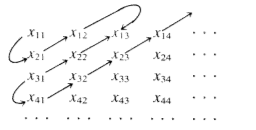
\includegraphics[width=0.7\linewidth]{images/fig-zig-zag-countable.png}
\caption*{\textbf{Figure 14.2.23:} Exercise 9}
\end{figure}
\end{divisionsolution}%
\section*{14.3 Automata, Finite-State Machines}
\addcontentsline{toc}{section}{14.3 Automata, Finite-State Machines}
\sectionmark{14.3 Automata, Finite-State Machines}
\subsection*{14.3 Exercises for Section 14.3}
\addcontentsline{toc}{subsection}{14.3 Exercises for Section 14.3}
\begin{divisionsolution}{14.3.1}{}{exercise-581}%
\hypertarget{p-5227}{}%
Draw a transition diagram for the vending machine described in Example~14.3.2.%
\par\smallskip%
\noindent\textbf{Answer}.\quad%
\hypertarget{p-5228}{}%
%
\begin{equation*}
\begin{array}{cccc}
x & s & Z(x,s) & t(x,s) \\
\textrm{ Deposit} 25\not{c} & \textrm{ Locked} & \textrm{ Nothing} & \textrm{ Select} \\
\textrm{ Deposit} 25\not{c} & \textrm{ Select} & \textrm{ Return} 25\not{c} & \textrm{ Select} \\
\textrm{ Press} S & \textrm{ Locked} & \textrm{ Nothing} & \textrm{ Locked} \\
\textrm{ Press} S & \textrm{ Select} & \textrm{ Dispense} S & \textrm{ Locked} \\
\textrm{ Press} P & \textrm{ Locked} & \textrm{ Nothing} & \textrm{ Locked} \\
\textrm{ Press} P & \textrm{ Select} & \textrm{ Dispense} P & \textrm{ Locked} \\
\textrm{ Press} B & \textrm{ Locked} & \textrm{ Nothing} & \textrm{ Locked} \\
\textrm{ Press} B & \textrm{ Select} & \textrm{ Dispense} B & \textrm{ Locked} \\
\end{array}
\end{equation*}
%
\begin{figure}
\centering
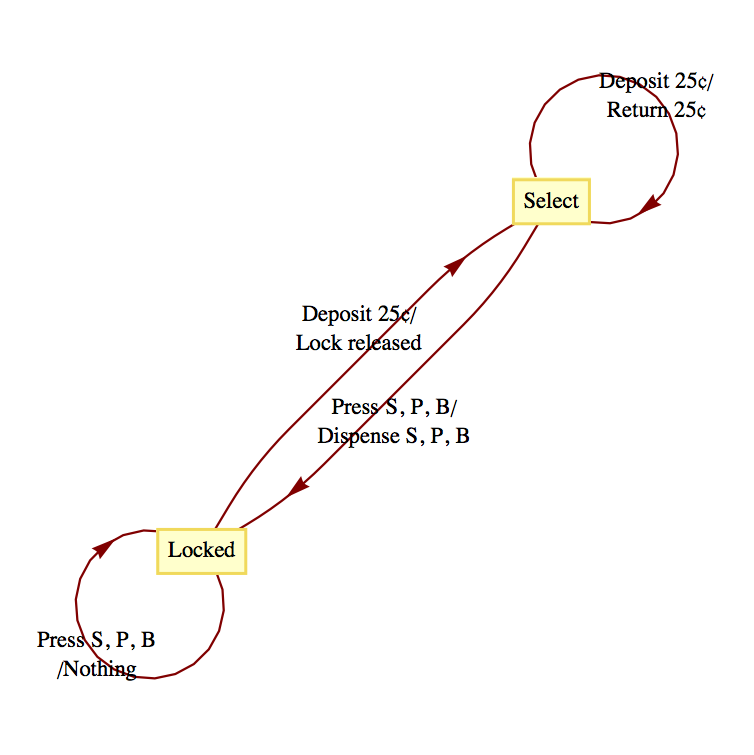
\includegraphics[width=0.7\linewidth]{images/fig-vending-diagram.png}
\caption*{\textbf{Figure 14.3.11:} Vending Machine Transitions}
\end{figure}
\end{divisionsolution}%
\begin{divisionsolution}{14.3.2}{}{exercise-582}%
\hypertarget{p-5229}{}%
Construct finite-state machines that recognize the regular languages that you identified in Section 14.2.%
\end{divisionsolution}%
\begin{divisionsolution}{14.3.3}{}{exercise-583}%
\hypertarget{p-5230}{}%
What is the input set for the binary adding machine in Example~14.3.9?%
\par\smallskip%
\noindent\textbf{Answer}.\quad%
\hypertarget{p-5231}{}%
\(\{000, 011, 101, 110, 111\}\)%
\end{divisionsolution}%
\begin{divisionsolution}{14.3.4}{}{exercise-584}%
\hypertarget{p-5232}{}%
What input sequence would be used to compute the sum of 1101 and 0111 (binary integers)? What would the output sequence be?%
\end{divisionsolution}%
\begin{divisionsolution}{14.3.5}{}{exercise-585}%
\hypertarget{p-5233}{}%
The Gray Code Decoder. The finite-state machine defined by the following figure has an interesting connection with the Gray Code.%
\begin{figure}
\centering
\includegraphics[width=0.7\linewidth]{images/fig-gray-code-decoder.png}
\caption*{\textbf{Figure 14.3.12:} Gray Code Decoder}
\end{figure}
\hypertarget{p-5234}{}%
Given a string \(x=x_1x_2\cdots  x_n\in B^n\), we may ask where \(x\) appears in \(G_n\). Starting in Copy state, the input string \(x\) will result in an output string \(z\in B^n\), which is the binary form of the position of \(x\) in \(G_n\).  Recall that positions are numbered from 0 to \(2^n-1\).\leavevmode%
\begin{enumerate}[label=(\alph*)]
\item\hypertarget{li-2380}{}\hypertarget{p-5235}{}%
In what positions \((0-31)\) do 10110, 00100, and 11111 appear in \(G_5\)?%
\item\hypertarget{li-2381}{}\hypertarget{p-5236}{}%
Prove that the Gray Code Decoder always works.%
\end{enumerate}
%
\par\smallskip%
\noindent\textbf{Answer}.\quad%
\hypertarget{p-5237}{}%
\leavevmode%
\begin{enumerate}[label=(\alph*)]
\item\hypertarget{li-2382}{}\hypertarget{p-5238}{}%
%
\begin{itemize}[label=\textbullet]
\item{}\hypertarget{p-5239}{}%
Input: 10110, Output: 11011 \(\Rightarrow\) 10110 is in position 27%
\item{}\hypertarget{p-5240}{}%
Input: 00100, Output: 00111 \(\Rightarrow\) 00100 is in position 7%
\item{}\hypertarget{p-5241}{}%
Input:11111, Output: 10101 \(\Rightarrow\) 11111 is in position 21%
\end{itemize}
%
\item\hypertarget{li-2386}{}\hypertarget{p-5242}{}%
Let \(x=x_1x_2\ldots  x_n\) and recall that for \(n\geq 1\), \(G_{n+1}=\left(
\begin{array}{c}
0G_n \\
1G_n^r \\
\end{array}
\right)\), where \(G_n^r\) is the reverse of \(G_n\). To prove that the Gray Code Decoder always works, let \(p(n)\) be the proposition ``Starting in Copy state,  \(x\)'s output is the position of \(x\) in \(G_n\);  and starting in Complement state, \(x\)'s output is the position of \(x\) in \(G_n^r\).''  That p(1) is true is easy to verify for both possible values of \(x\),  0 and 1.  Now assume that for some \(n\geq 1\), \(p(n)\) is true and consider \(x=x_1x_2\ldots  x_nx_{n+1}\).%
\par
\hypertarget{p-5243}{}%
If \(x_1=0\), \(x\)'s  output is a zero followed by the output for \(\left(x_2\ldots  x_nx_{n+1}\right)\) starting in Copy state. By the induction hypothesis, this is zero followed by the position of \(\left(x_2 \ldots  x_n x_{n+1}\right)\)  in \(G_n\), which is the position of \(x\) in  \(G_{n+1}\), by the definition of \(G\).%
\par
\hypertarget{p-5244}{}%
If  \(x_1=1\), \(x\)'s output is a one followed by the output for \(\left(x_2\ldots  x_nx_{n+1}\right)\) starting in Complement state.  By the induction hypothesis, this is one followed by the position of \(\left(x_2\ldots  x_nx_{n+1}\right)\)  in \(G_n^r\), which is the position of \(x\) in \(G_{n+1}\), by the definition of \(G\). \(\square\)%
\end{enumerate}
%
\end{divisionsolution}%
\section*{14.4 The Monoid of a Finite-State Machine}
\addcontentsline{toc}{section}{14.4 The Monoid of a Finite-State Machine}
\sectionmark{14.4 The Monoid of a Finite-State Machine}
\subsection*{14.4 Exercises for Section 14.4}
\addcontentsline{toc}{subsection}{14.4 Exercises for Section 14.4}
\begin{divisionsolution}{14.4.1}{}{exercise-586}%
\hypertarget{p-5262}{}%
For each of the transition diagrams in Figure~5, write out tables for their associated monoids. Identify the identity in terms of a string of positive length, if possible.%
\begin{figure}
\centering
\includegraphics[width=0.7\linewidth]{images/fig-exercise-14-4-1.png}
\caption*{\textbf{Figure 14.4.5:} Exercise 1}
\end{figure}
\par\smallskip%
\noindent\textbf{Hint}.\quad%
\hypertarget{p-5263}{}%
Where the output echoes the current state, the output can be ignored.%
\par\smallskip%
\noindent\textbf{Answer}.\quad%
\hypertarget{p-5264}{}%
\leavevmode%
\begin{enumerate}[label=(\alph*)]
\item\hypertarget{li-2387}{}\hypertarget{p-5265}{}%
\(\begin{array}{c|cccccc}
\textrm{ Input String} & a & b & c & aa & ab & ac \\
\hline
1 & (a,1) & (a,2) & (c,3) & (a,1) & (a,2) & (c,3) \\
2 & (a,2) & (a,1) & (c,3) & (a,2) & (a,1) & (c,3) \\
3 & (c,3) & (c,3) & (c,3) & (c,3) & (c,3) & (c,3) \\
\end{array}\) \(\begin{array}{c|cccccc}
\textrm{ Input String} & ba & bb & bc & ca & cb & cc \\
\hline
1 & (a,2) & (a,1) & (c,3) & (c,3) & (c,3) & (c,3) \\
2 & (a,1) & (a,2) & (c,3) & (c,3) & (c,3) & (c,3) \\
3 & (c,3) & (c,3) & (c,3) & (c,3) & (c,3) & (c,3) \\
\end{array}\)%
\par
\hypertarget{p-5266}{}%
We can see that \(T_aT_a= T_{\textrm{ \textit{aa}}}=T_a\),  \(T_aT_b= T_{\textrm{ \textit{ab}}}= T_b\), etc. Therefore, we have the following monoid:%
\begin{equation*}
\begin{array}{c|c}
& 
\begin{array}{ccc}
T_{a} & T_b &  T_b \\
\end{array}
\\
\hline
\begin{array}{c}
T_a \\
T_b \\
T_c \\
\end{array}
& 
\begin{array}{ccc}
T_a & T_b & T_c \\
T_b & T_a & T_c \\
T_c & T_c & T_c \\
\end{array}
\\
\end{array}
\end{equation*}
%
\par
\hypertarget{p-5267}{}%
Notice that \(T_a\) is the identity of this monoid.%
\item\hypertarget{li-2388}{}\hypertarget{p-5268}{}%
\(\begin{array}{c|cccccc}
\textrm{Input String} & 1 & 2  &  11 & 12 & 21 & 22 \\
\hline
A & C & B & A & D & D & A \\
B &  D & A & B & C & C & B \\
C & A & D & C & B & B & C \\
D &  B & C & D & A & A & D \\
\end{array}\)%
\par
\hypertarget{p-5269}{}%
\(\begin{array}{c|cccccccc}
\textrm{Input String} &111 & 112 & 121 & 122 & 211 & 212 & 221 & 222 \\
\hline
A & C & B & B & C & B & C & C & B \\
B  & D & A & A &  D & A & D & D & A \\
C  & B & C & C & B & C & B & B & C \\
D  & B & C & C & B & C & B & B & C \\
\end{array}\)%
\par
\hypertarget{p-5270}{}%
We have the following monoid:%
\begin{equation*}
\begin{array}{c|c}
& 
\begin{array}{cccc}
T_1 &  T_2 & T_{11} &  T_{12} \\
\end{array}
\\
\hline
\begin{array}{c}
T_1 \\
T_2 \\
T_{11} \\
T_{12} \\
\end{array}
& 
\begin{array}{cccc}
T_{11} & T_{12} & T_1 & T_2 \\
T_b & T_{11} & T_2 & T_1 \\
T_1 & T_2 & T_{11} & T_{12} \\
T_2 & T_1 & T_{12} & T_{11} \\
\end{array}
\\
\end{array}
\end{equation*}
%
\par
\hypertarget{p-5271}{}%
Notice that \(T_{11}\) is the identity of this monoid.%
\end{enumerate}
%
\end{divisionsolution}%
\begin{divisionsolution}{14.4.2}{}{exercise-587}%
\hypertarget{p-5272}{}%
What common monoids are isomorphic to the monoids obtained in the previous exercise?%
\end{divisionsolution}%
\begin{divisionsolution}{14.4.3}{}{exercise-588}%
\hypertarget{p-5273}{}%
Can two finite-state machines with nonisomorphic transition diagrams have isomorphic monoids?%
\par\smallskip%
\noindent\textbf{Answer}.\quad%
\hypertarget{p-5274}{}%
Yes, just consider the unit time delay machine of Figure~14.4.4. Its monoid is described by the table at the end of Section 14.4 where the \(T_{\lambda
}\) row and \(T_{\lambda }\) column are omitted. Next consider the machine in Figure~14.5.7. The monoid of this machine is:%
\begin{equation*}
\begin{array}{c|ccccccc}
& T_{\lambda } & T_0 & T_1 & T_{00} & T_{01} & T_{10} & T_{11} \\
\hline
T_{\lambda } & T_{\lambda } & T_0 & T_1 & T_{00} & T_{01} & T_{10} & T_{11} \\
\hline
T_0 & T_0 & T_{00} & T_{01} & T_{00} & T_{01} & T_{10} & T_{11} \\
T_1 & T_1 & T_{10} & T_{11} & T_{00} & T_{01} & T_{10} & T_{11} \\
T_{00} & T_{00} & T_{00} & T_{01} & T_{00} & T_{01} & T_{10} & T_{11} \\
T_{01} & T_{01} & T_{10} & T_{11} & T_{00} & T_{01} & T_{10} & T_{11} \\
T_{10} & T_{10} & T_{00} & T_{01} & T_{00} & T_{01} & T_{10} & T_{11} \\
T_{11} & T_{11} & T_{10} & T_{11} & T_{00} & T_{01} & T_{10} & T_{11} \\
\end{array}
\end{equation*}
%
\par
\hypertarget{p-5275}{}%
Hence both of these machines have the same monoid, however, their transition diagrams are nonisomorphic since the first has two vertices and the second has seven.%
\end{divisionsolution}%
\section*{14.5 The Machine of a Monoid}
\addcontentsline{toc}{section}{14.5 The Machine of a Monoid}
\sectionmark{14.5 The Machine of a Monoid}
\subsection*{14.5 Exercises for Section 14.5}
\addcontentsline{toc}{subsection}{14.5 Exercises for Section 14.5}
\begin{divisionsolution}{14.5.1}{}{exercise-589}%
\hypertarget{p-5282}{}%
Draw the transition diagrams for the machines of the following monoids:\leavevmode%
\begin{enumerate}[label=(\alph*)]
\item\hypertarget{li-2389}{}\hypertarget{p-5283}{}%
\(\left[\mathbb{Z}_4;+_4\right]\)%
\item\hypertarget{li-2390}{}\hypertarget{p-5284}{}%
The direct product of  \(\left[\mathbb{Z}_2;\times _2\right]\) with itself.%
\end{enumerate}
%
\par\smallskip%
\noindent\textbf{Answer}.\quad%
\leavevmode%
\begin{figure}
\centering
\includegraphics[width=0.7\linewidth]{images/fig-sol-14-5-1a.png}
\caption*{\textbf{Figure 14.5.8:} (a)}
\end{figure}
\begin{figure}
\centering
\includegraphics[width=0.7\linewidth]{images/fig-sol-14-5-1b.png}
\caption*{\textbf{Figure 14.5.9:} (b)}
\end{figure}
\end{divisionsolution}%
\begin{divisionsolution}{14.5.2}{}{exercise-590}%
\hypertarget{p-5285}{}%
Even though a monoid may be infinite, we can visualize it as an infinite-state machine provided that it is generated by a finite number of elements. For example, the monoid \(B^*\) is generated by 0 and 1. A section of its transition diagram can be obtained by allowing input only from the generating set. The monoid of integers under addition is generated by the set \(\{-1, 1\}\). The transition diagram for this monoid can be visualized by drawing a small portion of it, as in Figure~10. The same is true for the additive monoid of integers, as seen in Figure~11.%
\begin{figure}
\centering
\includegraphics[width=0.7\linewidth]{images/fig-exercise-14-5-2a.png}
\caption*{\textbf{Figure 14.5.10:} An infinite machine \(B^*\)}
\end{figure}
\begin{figure}
\centering
\includegraphics[width=0.7\linewidth]{images/fig-exercise-14-5-2b.png}
\caption*{\textbf{Figure 14.5.11:} An infinite machine \([\mathbb{Z};+]\)}
\end{figure}
\hypertarget{p-5286}{}%
\leavevmode%
\begin{enumerate}[label=(\alph*)]
\item\hypertarget{li-2391}{}\hypertarget{p-5287}{}%
Draw a transition diagram for \(\{a, b, c\}\)%
\item\hypertarget{li-2392}{}\hypertarget{p-5288}{}%
Draw a transition diagram for \([\mathbb{Z}\times \mathbb{Z};\textrm{componentwise addition}]\).%
\item\hypertarget{li-2393}{}\hypertarget{p-5289}{}%
Draw a transition diagram for \([\mathbb{Z};+]\) with generating set \(\{5,-2\}\).%
\end{enumerate}
%
\end{divisionsolution}%
\chapter*{15 Group Theory and Applications}
\addcontentsline{toc}{chapter}{15 Group Theory and Applications}
\chaptermark{15 Group Theory and Applications}
\section*{15.1 Cyclic Groups}
\addcontentsline{toc}{section}{15.1 Cyclic Groups}
\sectionmark{15.1 Cyclic Groups}
\subsection*{15.1 Exercises for Section 15.1}
\addcontentsline{toc}{subsection}{15.1 Exercises for Section 15.1}
\begin{divisionsolution}{15.1.1}{}{exercise-591}%
\hypertarget{p-5333}{}%
What generators besides 1 does \([\mathbb{Z}; +]\) have?%
\par\smallskip%
\noindent\textbf{Answer}.\quad%
\hypertarget{p-5334}{}%
The only other generator is \(-1\).%
\end{divisionsolution}%
\begin{divisionsolution}{15.1.2}{}{exercise-592}%
\hypertarget{p-5335}{}%
Without doing any multiplications, determine the number of generators of  \([\mathbb{Z}_{11}; +_{11}]\).%
\end{divisionsolution}%
\begin{divisionsolution}{15.1.3}{}{exercise-593}%
\hypertarget{p-5336}{}%
Prove that if \(\lvert G \rvert >2\) and \(G\) is cyclic, \(G\) has at least two generators.%
\par\smallskip%
\noindent\textbf{Answer}.\quad%
\hypertarget{p-5337}{}%
If  \(\lvert G \rvert = m\), \(m>2\), and \(G = \langle a \rangle\), then \(a\), \(a^2,\ldots\), \(a^{m-1}\) , \(a^m=e\) are distinct elements of \(G\). Furthermore, \(a^{-1}= a^{m-1}\neq a\),  If \(1 \leq k \leq m\), \(a^{-1}\) generates \(a^k\):%
\begin{equation*}
\begin{split}
\left(a^{-1}\right)^{m-k} &= \left(a^{m-1}\right)^{m-k}\\
& = a^{m^2-m-m k + k}\\
& =\left(a^m\right)^{m-k-1}*a^k\\
&= e*a^k=a^k\\
\end{split}
\end{equation*}
%
\par
\hypertarget{p-5338}{}%
Similarly, if \(G\) is infinite and \(G = \langle a\rangle\), then \(a^{-1}\) generates \(G\).%
\end{divisionsolution}%
\begin{divisionsolution}{15.1.4}{}{exercise-594}%
\hypertarget{p-5339}{}%
If you wanted to list the generators of \(\mathbb{Z}_n\) you would only have to test the first \(n/2\) positive integers. Why?%
\end{divisionsolution}%
\begin{divisionsolution}{15.1.5}{}{exercise-595}%
\hypertarget{p-5340}{}%
Which of the following groups are cyclic? Explain.\leavevmode%
\begin{enumerate}[label=(\alph*)]
\item\hypertarget{li-2394}{}\hypertarget{p-5341}{}%
\([\mathbb{Q}; +]\)%
\item\hypertarget{li-2395}{}\hypertarget{p-5342}{}%
\([\mathbb{R}^+;\cdot ]\)%
\item\hypertarget{li-2396}{}\hypertarget{p-5343}{}%
\([6\mathbb{Z}; +]\) where \(6\mathbb{Z} = \{6n |n \in  \mathbb{Z}\}\)%
\item\hypertarget{li-2397}{}\hypertarget{p-5344}{}%
\(\mathbb{Z} \times  \mathbb{Z}\)%
\item\hypertarget{li-2398}{}\hypertarget{p-5345}{}%
\(\mathbb{Z}_2\times  \mathbb{Z}_3 \times  \mathbb{Z}_{25}\)%
\end{enumerate}
%
\par\smallskip%
\noindent\textbf{Answer}.\quad%
\hypertarget{p-5346}{}%
\leavevmode%
\begin{enumerate}[label=(\alph*)]
\item\hypertarget{li-2399}{}\hypertarget{p-5347}{}%
No. Assume that \(q \in \mathbb{Q}\) generates \(\mathbb{Q}\). Then \(\langle q\rangle  = \{n q : n \in \mathbb{Z}\}\). But this gives us at most integer multiples of \(q\), not every element in \(\mathbb{Q}\).%
\item\hypertarget{li-2400}{}\hypertarget{p-5348}{}%
No. Similar reasoning to part a.%
\item\hypertarget{li-2401}{}\hypertarget{p-5349}{}%
Yes. 6 is a generator of \(6\mathbb{Z}\).%
\item\hypertarget{li-2402}{}\hypertarget{p-5350}{}%
No.%
\item\hypertarget{li-2403}{}\hypertarget{p-5351}{}%
Yes, \((1,1, 1)\) is a generator of the group.%
\end{enumerate}
%
\end{divisionsolution}%
\begin{divisionsolution}{15.1.6}{}{exercise-596}%
\hypertarget{p-5352}{}%
For each group and element, determine the order of the cyclic subgroup generated by the element:\leavevmode%
\begin{enumerate}[label=(\alph*)]
\item\hypertarget{li-2404}{}\hypertarget{p-5353}{}%
\(\mathbb{Z}_{25}\) , 15%
\item\hypertarget{li-2405}{}\hypertarget{p-5354}{}%
\(\mathbb{Z}_4\times \mathbb{Z}_9\) , \((2, 6)\) (apply Exercise 8)%
\item\hypertarget{li-2406}{}\hypertarget{p-5355}{}%
\(\mathbb{Z}_{64}\) , 2%
\end{enumerate}
%
\end{divisionsolution}%
\begin{divisionsolution}{15.1.7}{}{exercise-597}%
\hypertarget{p-5356}{}%
How can Theorem~15.1.13 be applied to list the generators of \(\mathbb{Z}_n\)? What are the generators of \(\mathbb{Z}_{25}\)? Of \(\mathbb{Z}_{256}\)?%
\par\smallskip%
\noindent\textbf{Answer}.\quad%
\hypertarget{p-5357}{}%
Theorem~15.1.13 implies that \(a\) generates \(\mathbb{Z}_n\) if and only if the greatest common divisor of \(n\) and \(a\) is 1. Therefore the list of generators of \(\mathbb{Z}_n\) are the integers in \(\mathbb{Z}_n\) that are relatively prime to \(n\). The generators of \(\mathbb{Z}_{25}\) are all of the nonzero elements except 5, 10, 15, and 20. The generators of \(\mathbb{Z}_{256}\) are the odd integers in \(\mathbb{Z}_{256}\)  since 256 is \(2^8\).%
\end{divisionsolution}%
\begin{divisionsolution}{15.1.8}{}{exercise-598}%
\hypertarget{p-5358}{}%
Prove that if the greatest common divisor of \(n\) and \(m\) is 1, then (1, 1) is a generator of \(\mathbb{Z}_n\times \mathbb{Z}_m\), and hence, \(\mathbb{Z}_n\times \mathbb{Z}_m\) is isomorphic to  \(\mathbb{Z}_{n m}\).%
\end{divisionsolution}%
\begin{divisionsolution}{15.1.9}{}{exercise-599}%
\hypertarget{p-5359}{}%
\leavevmode%
\begin{enumerate}[label=(\alph*)]
\item\hypertarget{li-2407}{}\hypertarget{p-5360}{}%
Illustrate how the fast adder can be used to add the numbers 21, 5, 7, and 15 using the isomorphism between \(\mathbb{Z}_{77}\) and \(\mathbb{Z}_7\times \mathbb{Z}_{11}\).%
\item\hypertarget{li-2408}{}\hypertarget{p-5361}{}%
If the same isomorphism is used to add the numbers 25, 26, and 40, what would the result be, why would it be incorrect, and how would the answer differ from the answer in part a?%
\end{enumerate}
%
\par\smallskip%
\noindent\textbf{Answer}.\quad%
\hypertarget{p-5362}{}%
\leavevmode%
\begin{enumerate}[label=(\alph*)]
\item\hypertarget{li-2409}{}\hypertarget{p-5363}{}%
\(\theta :\mathbb{Z}_{77} \to  \mathbb{Z}_7 \times  \mathbb{Z}_{11}\) maps the given integers as follows:%
\begin{equation*}
\begin{array}{ccc}
21 & \to  & (0,10) \\
5 & \to  & (5,5) \\
7 & \to  & (0,7) \\
15 & \to  & \underline{(1,4)} \\
\textrm{ sum}=48 & \leftarrow  & (6,4)=\textrm{ sum} \\
\end{array}
\end{equation*}
The final sum, 48, is obtained by using the facts that \(\theta ^{-1}(1,0) =22\) and \(\theta ^{-1}(0,1)=56\)%
\par
\hypertarget{p-5364}{}%
%
\begin{equation*}
\begin{split}
\theta^{-1}(6,4)= 6 \times_{77}\theta ^{-1}(1,0) + 4 \times_{77}\theta^{-1}(0,1)\\
& =6\times_{77}22 +_{77} 4\times_{77} 56\\
& =55 +_{77}70\\
& =48\\
\end{split}\text{.}
\end{equation*}
%
\item\hypertarget{li-2410}{}\hypertarget{p-5365}{}%
Using the same isomorphism:%
\begin{equation*}
\begin{array}{ccc}
25 & \to  & (4,3) \\
26 & \to  & (5,4) \\
40 & \to  & (5,7) \\
&   & \textrm{ sum}=(0,3) \\
\end{array}
\end{equation*}
%
\par
\hypertarget{p-5366}{}%
%
\begin{equation*}
\begin{split}
theta ^{-1}(0,3) &= 3 \times_{77}\theta ^{-1}(0,1)\\
& = 3\times_{77} 56\\ 
& =14\\
\end{split}\text{.}
\end{equation*}
%
\par
\hypertarget{p-5367}{}%
The actual sum is 91. Our result is incorrect, since 91 is not in \(\mathbb{Z}_{77}\).  Notice that 91 and 14 differ by 77. Any error that we get using this technique will be a multiple of 77.%
\end{enumerate}
%
\end{divisionsolution}%
\begin{divisionsolution}{15.1.10}{}{exercise-600}%
\hypertarget{p-5368}{}%
Prove that if \(G\). is a cyclic group of order \(n\) . with generator \(a\), and \(p, q \in  \{0, 1, \ldots , n - 1\}\), then \((p+q)a = \left(p+_nq\right)a\)%
\end{divisionsolution}%
\section*{15.2 Cosets and Factor Groups}
\addcontentsline{toc}{section}{15.2 Cosets and Factor Groups}
\sectionmark{15.2 Cosets and Factor Groups}
\subsection*{15.2 Exercises for Section 15.2}
\addcontentsline{toc}{subsection}{15.2 Exercises for Section 15.2}
\begin{divisionsolution}{15.2.1}{}{exercise-601}%
\hypertarget{p-5409}{}%
Consider \(\mathbb{Z}_{10}\) and the subsets of \(\mathbb{Z}_{10}\), \(\{0, 1, 2, 3, 4\}\) and \(\{5, 6, 7, 8, 9\}\). Why is the operation induced on these subsets by modulo 10 addition not well defined?%
\par\smallskip%
\noindent\textbf{Answer}.\quad%
\hypertarget{p-5410}{}%
An example of a valid correct answer: Call the subsets \(A\) and \(B\) respectively. If we choose \(0 \in A\) and \(5 \in B\) we get \(0 +_{10} 5 =5 \in  B\). On the other hand, if we choose \(3 \in A\) and \(8 \in  B\), we get \(3 +_{10} 8 = 1 \in  A\). Therefore, the induced operation is not well defined on \(\{A,B\}\).%
\end{divisionsolution}%
\begin{divisionsolution}{15.2.2}{}{exercise-602}%
\hypertarget{p-5411}{}%
Can you think of a group \(G\), with a subgroup \(H\) such that \(\lvert H\rvert  = 6\) and \(\lvert G/H\rvert  = 6\)? Is your answer unique?%
\end{divisionsolution}%
\begin{divisionsolution}{15.2.3}{}{exercise-603}%
\hypertarget{p-5412}{}%
For each group and subgroup, what is \(G/H\) isomorphic to?\leavevmode%
\begin{enumerate}[label=(\alph*)]
\item\hypertarget{li-2413}{}\hypertarget{p-5413}{}%
\(G = \mathbb{Z}_4 \times \mathbb{Z}_2\)  and  \(H = \langle (2, 0)\rangle\). Compare to Example~15.2.16.%
\item\hypertarget{li-2414}{}\hypertarget{p-5414}{}%
\(G = [\mathbb{C}; +]\)  and \(H = \mathbb{R}\).%
\item\hypertarget{li-2415}{}\hypertarget{p-5415}{}%
\(G\) = \(\mathbb{Z}_{20}\)  and  \(H = \langle 8\rangle\).%
\end{enumerate}
%
\par\smallskip%
\noindent\textbf{Answer}.\quad%
\hypertarget{p-5416}{}%
\leavevmode%
\begin{enumerate}[label=(\alph*)]
\item\hypertarget{li-2416}{}\hypertarget{p-5417}{}%
The four distinct cosets in \(G/H\) are \(H = \{(0, 0), (2, 0)\}\), \((1, 0) + H= \{(1,0),(3,0)\}\), \((0, 1) + H= \{(0,1),(2,1)\}\),  and \((1, 1) + H= \{(1,1),(3,1)\}\). None of these cosets generates \(G/H\); therefore \(G/H\) is not cyclic. Hence \(G/H\) must be isomorphic to \(\mathbb{Z}_2\times \mathbb{Z}_2\).%
\item\hypertarget{li-2417}{}\hypertarget{p-5418}{}%
The factor group is isomorphic to \([\mathbb{R}; +]\). Each coset of \(\mathbb{R}\) is a line in the complex plane that is parallel to the x-axis: \(\tau :\mathbb{C}/\mathbb{R}\to  \mathbb{R}\), where \(T(\{a + b i\mid a\in \mathbb{R}\}) = b\) is an isomorphism.%
\item\hypertarget{li-2418}{}\hypertarget{p-5419}{}%
\(\langle 8\rangle  = \{0, 4, 8, 12, 16\} \)\(\Rightarrow\)  \(\lvert \mathbb{Z}_{20}/\langle 8\rangle \rvert =4\). The four cosets are: \(\bar{0}\), \(\bar{1}\), \(\bar{2}\), and \(\bar{3}\). 1 generates all four cosets.  The factor group is isomorphic to \([\mathbb{Z}_4; +_4]\)  because \(\bar{1}\) is a generator.%
\end{enumerate}
%
\end{divisionsolution}%
\begin{divisionsolution}{15.2.4}{}{exercise-604}%
\hypertarget{p-5420}{}%
For each group and subgroup, what is \(G/H\) isomorphic to?\leavevmode%
\begin{enumerate}[label=(\alph*)]
\item\hypertarget{li-2419}{}\hypertarget{p-5421}{}%
\(G = \mathbb{Z}\times \mathbb{Z}\) and  \(H = \{(a, a) | a \in  \mathbb{Z}\}\).%
\item\hypertarget{li-2420}{}\hypertarget{p-5422}{}%
\(G = \left[\mathbb{R}^*; \cdot \right]\)  and  \(H = \{1, -1\}\).%
\item\hypertarget{li-2421}{}\hypertarget{p-5423}{}%
\(G =\mathbb{Z}_2{}^5\)  and \(H = \langle (1, 1, 1, 1, 1)\rangle\).%
\end{enumerate}
%
\end{divisionsolution}%
\begin{divisionsolution}{15.2.5}{}{exercise-605}%
\hypertarget{p-5424}{}%
Assume that \(G\) is a group, \(H \leq  G\), and \(a, b \in  G\).  Prove that \(a*H= b*H\)  if and only if  \(b^{-1}*a \in H\).%
\par\smallskip%
\noindent\textbf{Answer}.\quad%
\hypertarget{p-5425}{}%
%
\begin{equation*}
\begin{split}
a*H= b*H &\Leftrightarrow a \in b H\\
&\Leftrightarrow  a = b * h \textrm{      for  some }h \in H\\
&\Leftrightarrow b^{-1}*a = h \textrm{    for some }h \in H\\
& \Leftrightarrow  b^{-1}*a \in  H\\
\end{split}
\end{equation*}
%
\end{divisionsolution}%
\begin{divisionsolution}{15.2.6}{}{exercise-15-2-6}%
\hypertarget{p-5426}{}%
\leavevmode%
\begin{enumerate}[label=(\alph*)]
\item\hypertarget{li-2422}{}\hypertarget{p-5427}{}%
Real addition modulo \(r\),  \(r > 0\), can be described as the operation induced on cosets of \(\langle r\rangle\) by ordinary addition. Describe a system of distinguished representatives for the elements of \(\mathbb{R}/\langle r\rangle\).%
\item\hypertarget{li-2423}{}\hypertarget{p-5428}{}%
Consider the trigonometric function sine. Given that \(\sin (x+2\pi k) = \sin  x\) for all \(x\in \mathbb{R}\) and \(k\in \mathbb{Z}\), show how the distinguished representatives of \(\mathbb{R}/\langle 2\pi \rangle\) can be useful in developing an algorithm for calculating the sine of a number.%
\end{enumerate}
%
\end{divisionsolution}%
\begin{divisionsolution}{15.2.7}{}{exercise-607}%
\hypertarget{p-5429}{}%
Complete the proof of Theorem~15.2.8 by proving that if \(a \in  G\), \(\rho:H \to  a*H\) defined by \(\rho(h)= a*h\) is a bijection.%
\end{divisionsolution}%
\section*{15.3 Permutation Groups}
\addcontentsline{toc}{section}{15.3 Permutation Groups}
\sectionmark{15.3 Permutation Groups}
\subsection*{15.3.5 Exercises for Section 15.3}
\addcontentsline{toc}{subsection}{15.3.5 Exercises for Section 15.3}
\begin{divisionsolution}{15.3.5.1}{}{exercise-608}%
\hypertarget{p-5484}{}%
Given \(f=\left(
\begin{array}{cccc}
1 & 2 & 3 & 4 \\
2 & 1 & 4 & 3 \\
\end{array}
\right)\), \(g=\left(
\begin{array}{cccc}
1 & 2 & 3 & 4 \\
2 & 3 & 4 & 1 \\
\end{array}
\right)\), and \(h=\left(
\begin{array}{cccc}
1 & 2 & 3 & 4 \\
3 & 2 & 4 & 1 \\
\end{array}
\right)\), compute\leavevmode%
\begin{multicols}{2}
\begin{enumerate}[label=(\alph*)]
\item\hypertarget{li-2429}{}\hypertarget{p-5485}{}%
\(f\circ g\)%
\item\hypertarget{li-2430}{}\hypertarget{p-5486}{}%
\(g\circ h\)%
\item\hypertarget{li-2431}{}\hypertarget{p-5487}{}%
\((f\circ g)\circ h\)%
\item\hypertarget{li-2432}{}\hypertarget{p-5488}{}%
\(f\circ (g\circ h)\)%
\item\hypertarget{li-2433}{}\hypertarget{p-5489}{}%
\(h^{-1}\)%
\item\hypertarget{li-2434}{}\hypertarget{p-5490}{}%
\(h^{-1} \circ g\circ h\)%
\item\hypertarget{li-2435}{}\hypertarget{p-5491}{}%
\(f^{-1}\)%
\end{enumerate}
\end{multicols}
%
\par\smallskip%
\noindent\textbf{Answer}.\quad%
\hypertarget{p-5492}{}%
\leavevmode%
\begin{multicols}{2}
\begin{enumerate}[label=(\alph*)]
\item\hypertarget{li-2436}{}\hypertarget{p-5493}{}%
\(\left(
\begin{array}{cccc}
1 & 2 & 3 & 4 \\
1 & 4 & 3 & 2 \\
\end{array}
\right)\)%
\item\hypertarget{li-2437}{}\hypertarget{p-5494}{}%
\(\left(
\begin{array}{cccc}
1 & 2 & 3 & 4 \\
4 & 3 & 1 & 2 \\
\end{array}
\right)\)%
\item\hypertarget{li-2438}{}\hypertarget{p-5495}{}%
\(\left(
\begin{array}{cccc}
1 & 2 & 3 & 4 \\
3 & 4 & 2 & 1 \\
\end{array}
\right)\)%
\item\hypertarget{li-2439}{}\hypertarget{p-5496}{}%
\(\left(
\begin{array}{cccc}
1 & 2 & 3 & 4 \\
3 & 4 & 2 & 1 \\
\end{array}
\right)\)%
\item\hypertarget{li-2440}{}\hypertarget{p-5497}{}%
\(\left(
\begin{array}{cccc}
1 & 2 & 3 & 4 \\
4 & 2 & 1 & 3 \\
\end{array}
\right)\)%
\item\hypertarget{li-2441}{}\hypertarget{p-5498}{}%
\(\left(
\begin{array}{cccc}
1 & 2 & 3 & 4 \\
3 & 1 & 4 & 2 \\
\end{array}
\right)\)%
\item\hypertarget{li-2442}{}\hypertarget{p-5499}{}%
\(\left(
\begin{array}{cccc}
1 & 2 & 3 & 4 \\
2 & 1 & 4 & 3 \\
\end{array}
\right)\)%
\end{enumerate}
\end{multicols}
%
\end{divisionsolution}%
\begin{divisionsolution}{15.3.5.2}{}{exercise-609}%
\hypertarget{p-5500}{}%
Write \(f\), \(g\), and \(h\) from Exercise 1 as products of disjoint cycles and determine whether each is odd or even.%
\end{divisionsolution}%
\begin{divisionsolution}{15.3.5.3}{}{exercise-610}%
\hypertarget{p-5501}{}%
Do the left cosets of \(A_3=\left\{i,r_1,r_2\right\}\) over \(S_3\) form a group under the induced operation on left cosets of \(A_3\)? What about the left cosets of \(\left\langle f_1\right\rangle\)?%
\par\smallskip%
\noindent\textbf{Answer}.\quad%
\hypertarget{p-5502}{}%
\(S_3/A_3\) is a group of order two.   The operation on left cosets of \(H=\left\langle f_1\right\rangle\) is not well defined and so a group cannot be formed from left cosets of \(H\).%
\end{divisionsolution}%
\begin{divisionsolution}{15.3.5.4}{}{exercise-611}%
\hypertarget{p-5503}{}%
In its realization as permutations, the dihedral group \(D_3\) is equal to \(S_3\). Can you give a geometric explanation why?   Why isn't \(D_4\) equal to \(S_4\)?%
\end{divisionsolution}%
\begin{divisionsolution}{15.3.5.5}{}{exercise-d4-details}%
\hypertarget{p-5504}{}%
\leavevmode%
\begin{enumerate}[label=(\alph*)]
\item\hypertarget{li-2443}{}\hypertarget{p-5505}{}%
Complete the list of elements of \(D_4\) and write out a table for the group in its realization as symmetries.%
\item\hypertarget{li-2444}{}\hypertarget{p-5506}{}%
List the subgroups of \(D_4\) in a lattice diagram. Are they all cyclic? To what simpler groups are the subgroups of \(D_4\) isomorphic?%
\end{enumerate}
%
\par\smallskip%
\noindent\textbf{Answer}.\quad%
\hypertarget{p-5507}{}%
\(D_4 = \left\{i, r, r^2, r^3, f_1, f_2, f_3, f_4\right\}\) Where \(i\) is the identity function, \(r=\left(
\begin{array}{cccc}
1 & 2 & 3 & 4 \\
2 & 3 & 4 & 1 \\
\end{array}
\right)\), and%
\begin{equation*}
\begin{array}{cc}
f_1 =\left(
\begin{array}{cccc}
1 & 2 & 3 & 4 \\
4 & 3 & 2 & 1 \\
\end{array}
\right) & f_2 =\left(
\begin{array}{cccc}
1 & 2 & 3 & 4 \\
2 & 1 & 4 & 3 \\
\end{array}
\right) \\
f_3 =\left(
\begin{array}{cccc}
1 & 2 & 3 & 4 \\
3 & 2 & 1 & 4 \\
\end{array}
\right) & f_4 =\left(
\begin{array}{cccc}
1 & 2 & 3 & 4 \\
1 & 4 & 3 & 2 \\
\end{array}
\right) \\
\end{array}
\end{equation*}
The operation table for the group is%
\begin{equation*}
\begin{array}{c|c}
\circ  & \textrm{    }
\begin{array}{cccccccc}
i  & r  & r^2 & r^3  & f_1 &  f_2 & f_3 & f_4 \\
\end{array}
\\
\hline
\begin{array}{c}
i \\
r \\
r^2 \\
r^3 \\
f_1 \\
f_2 \\
f_3 \\
f_4 \\
\end{array}
& 
\begin{array}{cccccccc}
i & r & r^2 & r^3 & f_1 & f_2 & f_3 & f_4 \\
r & r^2 & r^3 & i & f_4 & f_3 & f_1 & f_2 \\
r^2 & r^3 & i & r & f_2 & f_1 & f_4 & f_3 \\
r^3 & i & r & r^2 & f_3 & f_4 & f_2 & f_1 \\
f_1 & f_3 & f_2 & f_4 & i & r^2 & r  & r^3 \\
f_2 & f_4 & f_1 & f_3 & r^2 & i & r^3 & r \\
f_3 & f_2 & f_4 & f_1 & r^3 & r & i & r^2 \\
f_4 & f_1 & f_3 & f_2 & r & r^3 & r^2 & i \\
\end{array}
\\
\end{array}
\end{equation*}
%
\par
\hypertarget{p-5508}{}%
A lattice diagram of its subgroups is%
\begin{figure}
\centering
\includegraphics[width=0.8\linewidth]{images/fig-d4-subgroups.png}
\caption*{\textbf{Figure 15.3.28:} Subgroups of \(D_4\)}
\end{figure}
\hypertarget{p-5509}{}%
All proper subgroups are cyclic except \(\left\{i,r^2,f_1,f_2\right\}\)\(\textrm{ }\textrm{ }\)and \(\left\{i,r^2,f_3,f_4\right\}\).  Each 2-element subgroup is isomorphic to \(\mathbb{Z}_2\) ; \(\left\{i,r,r^2,r^3\right\}\) is isomorphic to \(\mathbb{Z}_4\) ; and \(\left\{i,r^2,f_1,f_2\right\}\)\(\textrm{ }\textrm{ }\)and \(\left\{i,r^2,f_3,f_4\right\}\) are isomorphic to \(\mathbb{Z}_2\times \mathbb{Z}_2\).%
\end{divisionsolution}%
\begin{divisionsolution}{15.3.5.6}{}{exercise-613}%
\hypertarget{p-5510}{}%
Design a better letter-facing machine (see Example~15.3.26). How can you verify that a letter-facing machine does indeed check every corner of a letter? Can it be done on paper without actually sending letters through it?%
\end{divisionsolution}%
\begin{divisionsolution}{15.3.5.7}{}{exercise-614}%
\hypertarget{p-5511}{}%
Prove by induction that if \(r \geq  1\) and each \(t_i\), is a transposition, then  \(\left(t_1\circ t_2\circ \cdots \circ t_r\right){}^{-1}=t_r\circ \cdots \circ t_2\circ t_1\)%
\par\smallskip%
\noindent\textbf{Answer}.\quad%
\hypertarget{p-5512}{}%
One solution is to cite Exercise 3 at the end of Section 11.3. It can be directly applied to this problem. An induction proof of the problem at hand would be almost identical to the proof of the more general statement. \(\left(t_1t_2\cdots  t_r\right){}^{-1}= t_r{}^{-1}\cdots  t_2{}^{-1}t_1{}^{-1}\quad\textrm{ by Exercise 3 of  Section 11.3}\\
\\
\quad \quad = t_r\cdots  t_2t_1\textrm{                }\textrm{ since} \textrm{ each} \textrm{ transposition} \textrm{ inverts} \textrm{ itself}.\textrm{     }\blacksquare\)%
\end{divisionsolution}%
\begin{divisionsolution}{15.3.5.8}{}{exercise-615}%
\hypertarget{p-5513}{}%
How many elements are there in \(D_5\) ? Describe them geometrically.%
\end{divisionsolution}%
\begin{divisionsolution}{15.3.5.9}{}{exercise-616}%
\hypertarget{p-5514}{}%
Complete the proof of Theorem~15.3.9.%
\par\smallskip%
\noindent\textbf{Answer}.\quad%
\hypertarget{p-5515}{}%
Part I: That \(\lvert S_k \rvert  = k!\) follows from the Rule of Products.%
\par
\hypertarget{p-5516}{}%
Part II: Let  \(f\)  be the function defined on \(\{1,2,\textrm{ ...}, n\}\) by \(f(1)=2\), \(f(2)=3\),  \(f(3)=1\), and \(f(j) =j\)  for \(4\leq j\leq n\); and let \(g\) be defined by \(g(1) = 1\), \(g(2) = 3\), \(g(3) = 2\), and \(g(j) =j\)  for \(4\leq j\leq n\).  Note that \(f\) and \(g\) are elements of \(S_n\). Next, \((f\circ g)(1) = f(g(1)) = f(1) = 2\), while \((g \circ f)(1) = g(f(1)) = g(2) =
3\), hence  \(f\circ g\neq g\circ f\) and \(S_n\) is non-abelian for any \(n \geq  3\).%
\end{divisionsolution}%
\begin{divisionsolution}{15.3.5.10}{}{exercise-617}%
\hypertarget{p-5517}{}%
How many left cosets does \(A_n\), \(n\geq 2\) have?%
\end{divisionsolution}%
\begin{divisionsolution}{15.3.5.11}{}{exercise-618}%
\hypertarget{p-5518}{}%
Prove that  \(f\circ r= r^{n-1}\circ f\) in \(D_n\).%
\end{divisionsolution}%
\begin{divisionsolution}{15.3.5.12}{}{exercise-619}%
\hypertarget{p-5519}{}%
\leavevmode%
\begin{enumerate}[label=(\alph*)]
\item\hypertarget{li-2445}{}\hypertarget{p-5520}{}%
Prove that the tile puzzles corresponding to \(A_{16}\cap  \left\{ \left.f \in S_{16} \right| f(16) = 16\right\}\) are solvable.%
\item\hypertarget{li-2446}{}\hypertarget{p-5521}{}%
If  \(f(16)\neq  16\), how can you determine whether  \(f\)'s puzzle is solvable?%
\end{enumerate}
%
\end{divisionsolution}%
\begin{divisionsolution}{15.3.5.13}{}{exercise-620}%
\hypertarget{p-5522}{}%
\leavevmode%
\begin{enumerate}[label=(\alph*)]
\item\hypertarget{li-2447}{}\hypertarget{p-5523}{}%
Prove that \(S_3\) is isomorphic to \(R_3\),  the group of \(3 \times 3\) rook matrices (see Section 11.2 exercises).%
\item\hypertarget{li-2448}{}\hypertarget{p-5524}{}%
Prove that for each \(n \geq  2\), \(R_n\) is isomorphic to \(S_n\).%
\end{enumerate}
%
\par\smallskip%
\noindent\textbf{Answer}.\quad%
\hypertarget{p-5525}{}%
\leavevmode%
\begin{enumerate}[label=(\alph*)]
\item\hypertarget{li-2449}{}\hypertarget{p-5526}{}%
Both groups are non-abelian and of order 6; so they must be isomorphic, since only one such group exists up to isomorphism. The function \(\theta:S_3\to R_3\) defined by \(\begin{array}{cc}
\theta(i)=I & \theta\left(f_1\right)=F_1 \\
\theta\left(r_1\right)=R_1 & \theta\left(f_2\right)=F_2 \\
\theta\left(r_2\right)=R_2 & \theta\left(f_3\right)=F_3 \\
\end{array}\) is an isomorphism,%
\item\hypertarget{li-2450}{}\hypertarget{p-5527}{}%
Recall that since every function is a relation, it is natural to translate functions to Boolean matrices. Suppose that \(f\in S_n\). We will define its image, \(\theta(f)\), by%
\begin{equation*}
\theta(f)_{kj}=1\textrm{    }\Leftrightarrow \textrm{      }f(j)=k
\end{equation*}
That \(\theta\) is a bijection follows from the existence of \(\theta^{-1}\).   If \(A\) is a rook matrix,%
\begin{equation*}
\begin{split}
\theta^{-1}(A)(j)=k &\Leftrightarrow \textrm{ }\textrm{The } 1
\textrm{ in} \textrm{ column } j \textrm{ of } A \textrm{ appears} \textrm{ in} \textrm{ row } k \\
&\Leftrightarrow A_{kj}=1
\end{split}
\end{equation*}
For \(f,g\in  S_n\),%
\begin{equation*}
\begin{split}
\theta(f\circ g)_{kj}= 1 & \Leftrightarrow \textrm{ }(f \circ g)(j)=k\\
& \Leftrightarrow \exists  l\textrm{ such that }g(j)=l \textrm{ and } f(l)=k\\
& \Leftrightarrow \exists  l\textrm{ such that } \theta(g)_{lj}=1\textrm{ and }\textrm{}\theta(f)_{kl}=1\\
& \Leftrightarrow (\theta(f)\theta(g))_{kj}=1
\end{split}
\end{equation*}
Therefore,  \(\theta\) is an isomorphism.%
\end{enumerate}
%
\end{divisionsolution}%
\section*{15.4 Normal Subgroups and Group Homomorphisms}
\addcontentsline{toc}{section}{15.4 Normal Subgroups and Group Homomorphisms}
\sectionmark{15.4 Normal Subgroups and Group Homomorphisms}
\subsection*{15.4.3 Exercises for Section 15.4}
\addcontentsline{toc}{subsection}{15.4.3 Exercises for Section 15.4}
\begin{divisionsolution}{15.4.3.1}{}{exercise-621}%
\hypertarget{p-5590}{}%
Which of the following functions are homomorphisms? What are the kernels of those functions that are homomorphisms?\leavevmode%
\begin{enumerate}[label=(\alph*)]
\item\hypertarget{li-2468}{}\hypertarget{p-5591}{}%
\(\theta_1: \mathbb{R}^* \to  \mathbb{R}^+\) defined by \(\theta_1(a) =\left| a\right|\).%
\item\hypertarget{li-2469}{}\hypertarget{p-5592}{}%
\(\theta_2 : \mathbb{Z}_5 \rightarrow  \mathbb{Z}_2\) where \(\theta_2(n) =\left\{
\begin{array}{cc}
0 & \textrm{ if } n \textrm{ is even} \\
1 & \textrm{ if } n \textrm{ is odd} \\
\end{array}
\right.\).%
\item\hypertarget{li-2470}{}\hypertarget{p-5593}{}%
\(\theta_3 : \mathbb{R} \times  \mathbb{R} \rightarrow  \mathbb{R}\), where \(\theta_3(a, b) = a + b\).%
\item\hypertarget{li-2471}{}\hypertarget{p-5594}{}%
\(\theta_4 : S_4 \to S_4\) defined by \(\theta_4(f) = f\circ f=f^2\).%
\end{enumerate}
%
\par\smallskip%
\noindent\textbf{Answer}.\quad%
\hypertarget{p-5595}{}%
\leavevmode%
\begin{enumerate}[label=(\alph*)]
\item\hypertarget{li-2472}{}\hypertarget{p-5596}{}%
Yes, the kernel is \(\{1, -1\}\)%
\item\hypertarget{li-2473}{}\hypertarget{p-5597}{}%
No, since \(\theta _2\left(2 +_{5} 4\right)= \theta_2(1)=1\), but  \(\theta _2(2)+_2\theta_{2} (4)=0+_{2}0 =0\)%
\par
\hypertarget{p-5598}{}%
A follow-up might be to ask what happens if 5 is replaced with some other positive integer in this part.%
\item\hypertarget{li-2474}{}\hypertarget{p-5599}{}%
Yes, the kernel is \(\{(a, -a)| a \in \mathbb{R}\}\)%
\item\hypertarget{li-2475}{}\hypertarget{p-5600}{}%
No.  A counterexample, among many, would be to consider the two transpositions \(t_1=(1,3)\) and \(t_2=(1,2)\).  Compare \(\theta_4(t_1 \circ t_2)\) and \(\theta_4(t_1) \circ \theta_4(t_2)\).%
\end{enumerate}
%
\end{divisionsolution}%
\begin{divisionsolution}{15.4.3.2}{}{exercise-622}%
\hypertarget{p-5601}{}%
Which of the following functions are homomorphisms? What are the kernels of those functions that are homomorphisms?\leavevmode%
\begin{enumerate}[label=(\alph*)]
\item\hypertarget{li-2476}{}\hypertarget{p-5602}{}%
\(\alpha_1: M_{2\times 2}(\mathbb{R}) \rightarrow  \mathbb{R}\), defined by \(\alpha_1(A) = A_{11} A_{22} + A_{12} A_{21}\).%
\item\hypertarget{li-2477}{}\hypertarget{p-5603}{}%
\(\alpha_2 : \left(\mathbb{R}^*\right)^2 \rightarrow \mathbb{R}^*\) defined by \(\alpha_2 (a, b) = a b\).%
\item\hypertarget{li-2478}{}\hypertarget{p-5604}{}%
\(\alpha_3 : \left\{\left.A \in  M_{2\times 2}(\mathbb{R}) \right| \det  A \neq  0\right\} \to  \mathbb{R}^*\), where \(\alpha_3(A) = \det
A\).%
\item\hypertarget{li-2479}{}\hypertarget{p-5605}{}%
\(\alpha_4 : S_4\rightarrow  S_4\)  defined by \(\alpha_4(f)=f^{-1}\).%
\end{enumerate}
%
\end{divisionsolution}%
\begin{divisionsolution}{15.4.3.3}{}{exercise-623}%
\hypertarget{p-5606}{}%
Show that \(D_4\) has one proper normal subgroup, but that \(\langle (1,4)(2,3)\rangle\) is not normal.%
\par\smallskip%
\noindent\textbf{Answer}.\quad%
\hypertarget{p-5607}{}%
\(\langle r\rangle =\left\{i,r,r^2,r^3\right\}\) is a normal subgroup of \(D_4\). To see you could use the table given in the solution of Exercise~15.3.5.5 of Section 15.3 and verify that  \(a^{-1}h a \in \langle r\rangle\) for all \(a\in D_4\) and \(h\in \langle r\rangle\).   A more efficient approach is to prove the general theorem that if \(H\) is a subgroup \(G\) with exactly two distinct left cosets, than \(H\) is normal. \(\left\langle f_1\right\rangle\) is not a normal subgroup of \(D_4\).  \(\left\langle f_1\right\rangle =\left\{i,f_1\right\}\) and if we choose \(a = r\) and \(h=f_1\) then \(a^{-1}h a= r^3f_1r=f_2\notin \left\langle f_1\right\rangle\)%
\end{divisionsolution}%
\begin{divisionsolution}{15.4.3.4}{}{exercise-624}%
\hypertarget{p-5608}{}%
Prove that the function \(\Phi\) in Example~15.4.23 is a homomorphism.%
\end{divisionsolution}%
\begin{divisionsolution}{15.4.3.5}{}{exercise-625}%
\hypertarget{p-5609}{}%
Define the two functions  \(\alpha: \mathbb{Z}_2{}^3\rightarrow  \mathbb{Z}_2{}^4\)  and \(\beta :\mathbb{Z}_2{}^4\to \mathbb{Z}_2\) by \(\alpha\left(a_1,a_2,a_3 \right) = \left(a_1,a_2,a_3 ,a_1+_2 a_2+_2a_3\right)\), and \(\beta \left(b_1,b_2,b_3,b_4\right)=b_1+b_2+b_3+b_4\) Describe the function \(\beta \circ \alpha\). Is it a homomorphism?%
\par\smallskip%
\noindent\textbf{Answer}.\quad%
\hypertarget{p-5610}{}%
\((\beta \circ  \alpha )\left(a_1,a_2,a_3\right) = 0\)  and so \(\beta \circ \alpha\)  is the trivial homomorphism, but a homomorphism nevertheless.%
\end{divisionsolution}%
\begin{divisionsolution}{15.4.3.6}{}{exercise-626}%
\hypertarget{p-5611}{}%
Express \(\Phi\) in Example~15.4.23 in matrix form.%
\end{divisionsolution}%
\begin{divisionsolution}{15.4.3.7}{}{exercise-627}%
\hypertarget{p-5612}{}%
Prove that if \(G\) is an abelian group, then \(q(x) = x^2\) defines a homomorphism from \(G\) into \(G\).  Is \(q\) ever an isomorphism?%
\par\smallskip%
\noindent\textbf{Answer}.\quad%
\hypertarget{p-5613}{}%
Let \(x, y \in G\).%
\begin{equation*}
\begin{split}
q(x * y)  &= (x * y)^2\\ 
& = x*y*x*y \\
& = x*x*y*y \quad\textrm{ since } G \textrm{ is  abelian}\\
& =x^2*y^2 \\
&= q(x)*q(y)
\end{split}
\end{equation*}
Hence, \(q\) is a homomorphism. In order for \(q\) to be an isomorphism, it must be the case that no element other than the identity is its own inverse.%
\begin{equation*}
\begin{split}
x \in \textrm{Ker}(q) & \Leftrightarrow  q (x) = e \\
& \Leftrightarrow  x * x =e \\
& \Leftrightarrow   x^{-1}= x\\
\end{split}
\end{equation*}
%
\end{divisionsolution}%
\begin{divisionsolution}{15.4.3.8}{}{exercise-628}%
\hypertarget{p-5614}{}%
Prove that if \(\theta : G\rightarrow G'\) is a homomorphism, and \(H\triangleleft G\), then \(\theta(H) \triangleleft  \theta(G)\). Is it also true that \(\theta(H) \triangleleft  G'\)?%
\end{divisionsolution}%
\begin{divisionsolution}{15.4.3.9}{}{exercise-629}%
\hypertarget{p-5615}{}%
Prove that if \(\theta : G \rightarrow  G'\) is a homomorphism, and \(H' \leq  \theta(G)\), then \(\theta^{-1}(H') =\{a\in G| \theta
(a)\in H'\}\leq  G\).%
\par\smallskip%
\noindent\textbf{Answer}.\quad%
\hypertarget{p-5616}{}%
Proof: Recall that the inverse image of \(H'\) under \(\theta\) is \(\theta ^{-1}(H')=\{g\in G | \theta (g)\in H'\}\).%
\par
\hypertarget{p-5617}{}%
Closure:   Let \(g_1, g_2\in \theta ^{-1}(H')\), then \(\theta \left(g_1\right),\theta \left(g_2\right)\in H'\).  Since \(H'\) is a subgroup of \(G'\),%
\begin{equation*}
\theta\left(g_1\right)\diamond \theta\left(g_2\right)=\theta\left(g_1*g_2\right)\in H' \Rightarrow  g_1*g_2\in \theta^{-1}(H')
\end{equation*}
%
\par
\hypertarget{p-5618}{}%
Identity: By Theorem~15.4.14(a), \(e \in \theta ^{-1}(H')\).%
\par
\hypertarget{p-5619}{}%
Inverse: Let \(a\in \theta ^{-1}(H')\) . Then \(\theta (a)\in H'\) and by Theorem~15.4.14(b), \(\theta (a)^{-1}= \theta \left(a^{-1}\right)\in H'\) and so \(a^{-1}\in \theta ^{-1}(H')\).%
\end{divisionsolution}%
\begin{divisionsolution}{15.4.3.10}{}{exercise-630}%
\hypertarget{p-5620}{}%
Following up on Example~15.4.10,  prove that \(A_5\) is a simple group; i. e., it has no proper normal subgroups.\leavevmode%
\begin{enumerate}[label=(\alph*)]
\item\hypertarget{li-2480}{}\hypertarget{p-5621}{}%
Make a list of  the different cycle structures that occur in \(A_5\) and how many elements have those structures.%
\item\hypertarget{li-2481}{}\hypertarget{p-5622}{}%
Within each set of permutations with different cycle structures, identify which subsets are closed with respect to the conjugation operation. With this you will have a partition of \(A_5\) into conjugate classes.  where for each class \(C\), \(f, g\in  C\)   if and only if   \(\exists  \phi  \in A_5\)  such that  \(\phi ^{-1}\circ f\circ  \phi  = g\).%
\item\hypertarget{li-2482}{}\hypertarget{p-5623}{}%
Use the fact that a normal subgroup of \(A_5\) needs to be a union of conjugate classes and verify that no such union exists.%
\end{enumerate}
%
\end{divisionsolution}%
\section*{15.5 Coding Theory, Group Codes}
\addcontentsline{toc}{section}{15.5 Coding Theory, Group Codes}
\sectionmark{15.5 Coding Theory, Group Codes}
\subsection*{15.5.3 Exercises for Section 15.5}
\addcontentsline{toc}{subsection}{15.5.3 Exercises for Section 15.5}
\begin{divisionsolution}{15.5.3.1}{}{exercise-631}%
\hypertarget{p-5653}{}%
If the error-detecting code is being used, how would you act on the following received blocks?\leavevmode%
\begin{enumerate}[label=(\alph*)]
\item\hypertarget{li-2483}{}\hypertarget{p-5654}{}%
\((1, 0, 1, 1)\)%
\item\hypertarget{li-2484}{}\hypertarget{p-5655}{}%
\((1, 1, 1, 1)\)%
\item\hypertarget{li-2485}{}\hypertarget{p-5656}{}%
\((0, 0, 0, 0)\)%
\end{enumerate}
%
\par\smallskip%
\noindent\textbf{Answer}.\quad%
\hypertarget{p-5657}{}%
\leavevmode%
\begin{enumerate}[label=(\alph*)]
\item\hypertarget{li-2486}{}\hypertarget{p-5658}{}%
Error detected, since an odd number of 1's was received; ask for retransmission.%
\item\hypertarget{li-2487}{}\hypertarget{p-5659}{}%
No error detected; accept this block.%
\item\hypertarget{li-2488}{}\hypertarget{p-5660}{}%
No error detected; accept this block.%
\end{enumerate}
%
\end{divisionsolution}%
\begin{divisionsolution}{15.5.3.2}{}{exercise-632}%
\hypertarget{p-5661}{}%
Express the encoding and decoding functions for the error-detecting code using matrices.%
\end{divisionsolution}%
\begin{divisionsolution}{15.5.3.3}{}{exercise-633}%
\hypertarget{p-5662}{}%
If the error-correcting code from this section is being used, how would you decode the following blocks? Expect an error that cannot be fixed with one of these.\leavevmode%
\begin{enumerate}[label=(\alph*)]
\item\hypertarget{li-2489}{}\hypertarget{p-5663}{}%
\((1,0,0,0,1,1)\)%
\item\hypertarget{li-2490}{}\hypertarget{p-5664}{}%
\((1,0,1,0,1,1)\)%
\item\hypertarget{li-2491}{}\hypertarget{p-5665}{}%
\((0,1,1,1,1,0)\)%
\item\hypertarget{li-2492}{}\hypertarget{p-5666}{}%
\((0,0,0,1,1,0)\)%
\item\hypertarget{li-2493}{}\hypertarget{p-5667}{}%
\((1,0,0,0,0,1)\)%
\item\hypertarget{li-2494}{}\hypertarget{p-5668}{}%
\((1,0,0,1,0,0)\)%
\end{enumerate}
%
\par\smallskip%
\noindent\textbf{Answer}.\quad%
\hypertarget{p-5669}{}%
\leavevmode%
\begin{enumerate}[label=(\alph*)]
\item\hypertarget{li-2495}{}\hypertarget{p-5670}{}%
Syndrome = \((1,0,1)\). Corrected coded message is \((1,1,0,0,1,1)\) and original message was \((1, 1, 0)\).%
\item\hypertarget{li-2496}{}\hypertarget{p-5671}{}%
Syndrome = \((1,1,0)\). Corrected coded message is \((0,0,1,0,1,1)\) and original message was \((0, 0, 1)\).%
\item\hypertarget{li-2497}{}\hypertarget{p-5672}{}%
Syndrome = \((0,0,0)\).  No error, coded message is \((0,1,1,1,1,0)\) and original message was \((0, 1, 1)\).%
\item\hypertarget{li-2498}{}\hypertarget{p-5673}{}%
Syndrome = \((1, 1,0)\). Corrected coded message is \((1,0,0,1,1,0)\) and original message was \((1, 0, 0)\).%
\item\hypertarget{li-2499}{}\hypertarget{p-5674}{}%
Syndrome = \((1,1,1)\). This syndrome occurs only if two bits have been switched. No reliable correction is possible.%
\item\hypertarget{li-2500}{}\hypertarget{p-5675}{}%
Syndrome = \((0,1,0)\). Corrected coded message is \((1,0,0,1,1,0)\) and original message was \((1, 0, 0)\).%
\end{enumerate}
%
\end{divisionsolution}%
\begin{divisionsolution}{15.5.3.4}{}{exercise-634}%
\hypertarget{p-5676}{}%
Describe how the triple-repetition code with encoding function, \(e:\mathbb{Z}_2\to \mathbb{Z}_2{}^3\), where \(e\left(a_1\right) = \left(a_1,a_1,a_1\right)\) can allow us to correct a single error. What is the probability of success for the \(p = 0.001\), 3000-bit situation?  What are the generator and parity-check matrices for this code?%
\end{divisionsolution}%
\begin{divisionsolution}{15.5.3.5}{}{exercise-635}%
\hypertarget{p-5677}{}%
Consider the  linear code defined by the generator matrix%
\begin{equation*}
G=\left(
\begin{array}{cccc}
1 & 0 & 1 & 0 \\
0 & 1 & 1 & 1 \\
\end{array}
\right)
\end{equation*}
%
\par
\hypertarget{p-5678}{}%
\leavevmode%
\begin{enumerate}[label=(\alph*)]
\item\hypertarget{li-2501}{}\hypertarget{p-5679}{}%
What size blocks does this code encode and what is the length of the code words?%
\item\hypertarget{li-2502}{}\hypertarget{p-5680}{}%
What are the code words for this code?%
\item\hypertarget{li-2503}{}\hypertarget{p-5681}{}%
With this code, can you detect single bit errors?  Can you correct all, some, or no single bit errors?%
\end{enumerate}
%
\par\smallskip%
\noindent\textbf{Answer}.\quad%
\hypertarget{p-5682}{}%
Let \(G\) be the \(9 \times 10\) matrix obtained by augmenting the \(9\times 9\) identity matrix with a column of ones. The function \(e:\mathbb{Z}_2{}^9\to \mathbb{Z}_2{}^{10}\)  defined by \(e(a) = a G\) will allow us to detect single errors, since \(e(a)\) will always have an even number of ones.%
\end{divisionsolution}%
\begin{divisionsolution}{15.5.3.6}{Rectangular codes.}{exercise-636}%
\hypertarget{p-5683}{}%
To build a rectangular code, you partition your message into blocks of length \(m\) and then factor \(m\) into \(k_1\cdot k_2\)  and arrange the bits in a  \(k_1 \times k_2\) rectangular array as in the figure below.  Then you add parity bits along the right side and bottom of the rows and columns.   The code word is then read row by row.%
\begin{equation*}
\begin{array}{cccccc}
\blacksquare  & \blacksquare  & \blacksquare  & \cdots  & \blacksquare  & \square  \\
\blacksquare  & \blacksquare  & \blacksquare  & \cdots  & \blacksquare  & \square  \\
\vdots  & \vdots  & \vdots  &   & \vdots  & \vdots  \\
\blacksquare  & \blacksquare  & \blacksquare  & \cdots  & \blacksquare  & \square  \\
\square  & \square  & \square  & \cdots  & \square  &   \\
\end{array}  \quad \begin{array}{c}
\textrm{      }\blacksquare  = \textrm{ message} \textrm{ bit} \\
\square  =\textrm{ parity} \textrm{ bit} \\
\end{array}
\end{equation*}
%
\par
\hypertarget{p-5684}{}%
For example, if \(m\) is 4, then our only choice is a 2 by 2 array.  The message 1101 would be encoded as%
\begin{equation*}
\begin{array}{cc|c}
1 & 1 & 0\\
0 & 1 & 1\\
\hline
1 & 0 &\\
\end{array}
\end{equation*}
and the code word is the string 11001110.%
\par
\hypertarget{p-5685}{}%
\leavevmode%
\begin{enumerate}[label=(\alph*)]
\item\hypertarget{li-2504}{}\hypertarget{p-5686}{}%
Suppose that you were sent four bit messages using this code and you received the following strings.  What were the messages, assuming no more than one error in the transmission of coded data?%
\begin{multicols}{3}
\begin{enumerate}[label=(\roman*)]
\item\hypertarget{li-2505}{}\hypertarget{p-5687}{}%
11011000%
\item\hypertarget{li-2506}{}\hypertarget{p-5688}{}%
01110010%
\item\hypertarget{li-2507}{}\hypertarget{p-5689}{}%
10001111%
\end{enumerate}
\end{multicols}
%
\item\hypertarget{li-2508}{}\hypertarget{p-5690}{}%
If you encoded \(n^2\) bits in this manner, what would be the rate of the code?%
\item\hypertarget{li-2509}{}\hypertarget{p-5691}{}%
Rectangular codes are linear codes.  For the 3 by 2 rectangular code, what are the generator and parity check matrices?%
\end{enumerate}
%
\end{divisionsolution}%
\chapter*{16 An Introduction to Rings and Fields}
\addcontentsline{toc}{chapter}{16 An Introduction to Rings and Fields}
\chaptermark{16 An Introduction to Rings and Fields}
\section*{16.1 Rings, Basic Definitions and Concepts}
\addcontentsline{toc}{section}{16.1 Rings, Basic Definitions and Concepts}
\sectionmark{16.1 Rings, Basic Definitions and Concepts}
\subsection*{16.1.6 Exercises for Section 16.1}
\addcontentsline{toc}{subsection}{16.1.6 Exercises for Section 16.1}
\begin{divisionsolution}{16.1.6.1}{}{exercise-637}%
\hypertarget{p-5772}{}%
Review the definition of rings to show that the following are rings. The operations involved are the usual operations defined on the sets. Which of these rings are commutative? Which are rings with unity? For the rings with unity, determine the unity and all units.\leavevmode%
\begin{enumerate}[label=(\alph*)]
\item\hypertarget{li-2533}{}\hypertarget{p-5773}{}%
\([\mathbb{Z};+,\cdot ]\)%
\item\hypertarget{li-2534}{}\hypertarget{p-5774}{}%
\([\mathbb{C};+,\cdot ]\)%
\item\hypertarget{li-2535}{}\hypertarget{p-5775}{}%
\([\mathbb{Q};+,\cdot ]\)%
\item\hypertarget{li-2536}{}\hypertarget{p-5776}{}%
\(\left[M_{2\times 2}(\mathbb{R});+, \cdot \right]\)%
\item\hypertarget{li-2537}{}\hypertarget{p-5777}{}%
\(\left[\mathbb{Z}_2;+_2,\times_2\right]\)%
\end{enumerate}
%
\par\smallskip%
\noindent\textbf{Answer}.\quad%
\hypertarget{p-5778}{}%
All but ring d are commutative. All of the rings have a unity element. The number 1 is the unity for all of the rings except d. The unity for \(M_{2\times 2}(\mathbb{R})\) is the two by two identity matrix. The units are as follows:\leavevmode%
\begin{multicols}{2}
\begin{enumerate}[label=(\alph*)]
\item\hypertarget{li-2538}{}\hypertarget{p-5779}{}%
\(\{1, -1\}\)%
\item\hypertarget{li-2539}{}\hypertarget{p-5780}{}%
\(\mathbb{C}^*\)%
\item\hypertarget{li-2540}{}\hypertarget{p-5781}{}%
\(\mathbb{Q}^*\)%
\item\hypertarget{li-2541}{}\hypertarget{p-5782}{}%
\(\left\{A \left| A_{11}A_{22}-A_{12}A_{21}\neq 0\right.\right\}\)%
\item\hypertarget{li-2542}{}\hypertarget{p-5783}{}%
\(\{1\}\)%
\end{enumerate}
\end{multicols}
%
\end{divisionsolution}%
\begin{divisionsolution}{16.1.6.2}{}{exercise-638}%
\hypertarget{p-5784}{}%
Follow the instructions for Exercise 1 and the following rings:\leavevmode%
\begin{multicols}{2}
\begin{enumerate}[label=(\alph*)]
\item\hypertarget{li-2543}{}\hypertarget{p-5785}{}%
\(\left[\mathbb{Z}_6;+_6,\times_6\right]\)%
\item\hypertarget{li-2544}{}\hypertarget{p-5786}{}%
\(\left[\mathbb{Z}_5;+_5,\times_5\right]\)%
\item\hypertarget{li-2545}{}\hypertarget{p-5787}{}%
\(\left[\mathbb{Z}_2{}^3;+,\cdot \right]\)%
\item\hypertarget{li-2546}{}\hypertarget{p-5788}{}%
\(\left[\mathbb{Z}_8; +_8 , \times_8 \right]\)%
\item\hypertarget{li-2547}{}\hypertarget{p-5789}{}%
\([\mathbb{Z} \times \mathbb{Z}; +, \cdot ]\)%
\item\hypertarget{li-2548}{}\hypertarget{p-5790}{}%
\(\left[\mathbb{R}^2; +, \cdot \right]\)%
\end{enumerate}
\end{multicols}
%
\end{divisionsolution}%
\begin{divisionsolution}{16.1.6.3}{}{exercise-639}%
\hypertarget{p-5791}{}%
Show that the following pairs of rings are not isomorphic:\leavevmode%
\begin{enumerate}[label=(\alph*)]
\item\hypertarget{li-2549}{}\hypertarget{p-5792}{}%
\([\mathbb{Z};+,\cdot ]\) and \(\left[M_{2\times 2}(\mathbb{Z});+,\cdot \right]\)%
\item\hypertarget{li-2550}{}\hypertarget{p-5793}{}%
\([3\mathbb{Z};+, \cdot ]\) and \([4\mathbb{Z};+, \cdot ]\).%
\end{enumerate}
%
\par\smallskip%
\noindent\textbf{Answer}.\quad%
\hypertarget{p-5794}{}%
\leavevmode%
\begin{enumerate}[label=(\alph*)]
\item\hypertarget{li-2551}{}\hypertarget{p-5795}{}%
Consider commutativity%
\item\hypertarget{li-2552}{}\hypertarget{p-5796}{}%
Solve \(x ^2=3x\) in both rings.%
\end{enumerate}
%
\end{divisionsolution}%
\begin{divisionsolution}{16.1.6.4}{}{exercise-640}%
\hypertarget{p-5797}{}%
Show that the following pairs of rings are not isomorphic:\leavevmode%
\begin{enumerate}[label=(\alph*)]
\item\hypertarget{li-2553}{}\hypertarget{p-5798}{}%
\([\mathbb{R}; +, \cdot ]\) and \([\mathbb{Q};+, \cdot ]\).%
\item\hypertarget{li-2554}{}\hypertarget{p-5799}{}%
\(\left[\mathbb{Z}_2 \times  \mathbb{Z}_2; +,\cdot \right]\)and \(\left[\mathbb{Z}_4; +, \cdot \right]\).%
\end{enumerate}
%
\end{divisionsolution}%
\begin{divisionsolution}{16.1.6.5}{}{exercise-641}%
\hypertarget{p-5800}{}%
\leavevmode%
\begin{enumerate}[label=(\alph*)]
\item\hypertarget{li-2555}{}\hypertarget{p-5801}{}%
Show that \(3\mathbb{Z}\) is a subring of the ring \([\mathbb{Z}; +, \cdot]\)%
\item\hypertarget{li-2556}{}\hypertarget{p-5802}{}%
Find all subrings of \(\mathbb{Z}_8\).%
\item\hypertarget{li-2557}{}\hypertarget{p-5803}{}%
Find all subrings of \(\mathbb{Z}_2 \times \mathbb{Z}_2\).%
\end{enumerate}
%
\par\smallskip%
\noindent\textbf{Answer}.\quad%
\hypertarget{p-5804}{}%
\leavevmode%
\begin{enumerate}[label=(\alph*)]
\item\hypertarget{li-2558}{}\hypertarget{p-5805}{}%
We already know that \(3\mathbb{Z}\) is a subgroup of the group \(\mathbb{Z}\). We need only show that \(3\mathbb{Z}\) is closed with respect to multiplication.  Let \(3m, 3n \in  3\mathbb{Z}\). \((3m)(3n) = 3(3m n) \in  3\mathbb{Z}\), since \(3 m n \in \mathbb{Z}\).%
\item\hypertarget{li-2559}{}\hypertarget{p-5806}{}%
The proper subrings are \(\{0, 2, 4, 6\}\) and \(\{0, 4\}\); while \(\{0\}\) and \(\mathbb{Z}_8\) are improper subrings.%
\item\hypertarget{li-2560}{}\hypertarget{p-5807}{}%
The proper subrings are \(\{00, 01\}\), \(\{00, 10\}\), and \(\{00,11\}\): while \(\{00\}\) and \(\mathbb{Z}_2\times \mathbb{Z}_2\) are improper subrings.%
\end{enumerate}
%
\end{divisionsolution}%
\begin{divisionsolution}{16.1.6.6}{}{exercise-642}%
\hypertarget{p-5808}{}%
Verify the validity of Theorem~16.1.22 by finding examples of elements \(a\), \(b\), and \(c\),  \(a  \neq   0\) in the following rings, where \(a \cdot b = a \cdot  c\) and yet  \(b \neq  c\):\leavevmode%
\begin{enumerate}[label=(\alph*)]
\item\hypertarget{li-2561}{}\hypertarget{p-5809}{}%
\(\mathbb{Z}_8\)%
\item\hypertarget{li-2562}{}\hypertarget{p-5810}{}%
\(M_{2\times 2}(\mathbb{R})\)%
\item\hypertarget{li-2563}{}\hypertarget{p-5811}{}%
\(\mathbb{Z}_2{}^2\)%
\end{enumerate}
%
\end{divisionsolution}%
\begin{divisionsolution}{16.1.6.7}{}{exercise-643}%
\hypertarget{p-5812}{}%
\leavevmode%
\begin{enumerate}[label=(\alph*)]
\item\hypertarget{li-2564}{}\hypertarget{p-5813}{}%
Determine all solutions of the equation \(x^2 - 5x + 6 = 0\) in \(\mathbb{Z}\).  Can there be any more than two solutions to this equation (or any quadratic equation) in \(\mathbb{Z}\)?%
\item\hypertarget{li-2565}{}\hypertarget{p-5814}{}%
Find all solutions of the equation in part a in \(\mathbb{Z}_{12}\). Why are there more than two solutions?%
\end{enumerate}
%
\par\smallskip%
\noindent\textbf{Answer}.\quad%
\hypertarget{p-5815}{}%
\leavevmode%
\begin{enumerate}[label=(\alph*)]
\item\hypertarget{li-2566}{}\hypertarget{p-5816}{}%
The left-hand side of the equation factors into the product \((x-2)(x-3)\). Since \(\mathbb{Z}\) is an integral domain, \(x = 2\) and \(x =3\) are the only possible solutions.%
\item\hypertarget{li-2567}{}\hypertarget{p-5817}{}%
Over \(\mathbb{Z}_{12}\), 2, 3, 6, and 11 are solutions. Although the equation factors into \((x-2)(x-3)\), this product can be zero without making \(x\) either 2 or 3. For example. If \(x\) = 6 we get  \((6-2)\times _{12}(6-3)=4 \times _{12}3 = 0\).  Notice that  4 and 3 are zero divisors.%
\end{enumerate}
%
\end{divisionsolution}%
\begin{divisionsolution}{16.1.6.8}{}{exercise-644}%
\hypertarget{p-5818}{}%
Solve the equation \(x^2 +4x + 4 = 0\) in the following rings. Interpret 4 as \(1 + 1 + 1 + 1\), where 1 is the unity of the ring.\leavevmode%
\begin{enumerate}[label=(\alph*)]
\item\hypertarget{li-2568}{}\hypertarget{p-5819}{}%
in  \(\mathbb{Z}_8\)%
\item\hypertarget{li-2569}{}\hypertarget{p-5820}{}%
in \(M_{2\times 2}(\mathbb{R})\)%
\item\hypertarget{li-2570}{}\hypertarget{p-5821}{}%
in  \(\mathbb{Z}\)%
\item\hypertarget{li-2571}{}\hypertarget{p-5822}{}%
in  \(\mathbb{Z}_3\)%
\end{enumerate}
%
\end{divisionsolution}%
\begin{divisionsolution}{16.1.6.9}{}{exercise-645}%
\hypertarget{p-5823}{}%
The relation ``is isomorphic to'' on rings is an equivalence relation. Explain the meaning of this statement.%
\par\smallskip%
\noindent\textbf{Answer}.\quad%
\hypertarget{p-5824}{}%
Let \(R_1\), \(R_2\), and \(R_3\)  be any rings, then\leavevmode%
\begin{enumerate}[label=(\alph*)]
\item\hypertarget{li-2572}{}\hypertarget{p-5825}{}%
\(R_1\) is isomorphic to \(R_1\) and so ``is isomorphic to'' is a reflexive relation on rings.%
\item\hypertarget{li-2573}{}\hypertarget{p-5826}{}%
\(R_1\) is isomorphic to \(R_2\)  \(\Rightarrow\) \(R_2\) is isomorphic to \(R_1\), and so ``is isomorphic to'' is a symmetric relation on rings,%
\item\hypertarget{li-2574}{}\hypertarget{p-5827}{}%
\(R_1\) is isomorphic to \(R_2\), and \(R_2\) is isomorphic to \(R_3\) implies that \(R_1\) is isomorphic to \(R_3\), and so ``is isomorphic to'' is a transitive relation on rings.%
\end{enumerate}
We haven't proven these properties here, just stated them.  The combination of these observations implies that ``is isomorphic to'' is an equivalence relation on rings.%
\end{divisionsolution}%
\begin{divisionsolution}{16.1.6.10}{}{exercise-646}%
\hypertarget{p-5828}{}%
\leavevmode%
\begin{enumerate}[label=(\alph*)]
\item\hypertarget{li-2575}{}\hypertarget{p-5829}{}%
Let \(R_1\), \(R_2\), \(\ldots\), \(R_n\) be rings. Prove the multiplicative, associative, and distributive laws for the ring%
\begin{equation*}
R=\underset{i=1}{\overset{n}{\times }}R_i
\end{equation*}
%
\item\hypertarget{li-2576}{}\hypertarget{p-5830}{}%
If each of the \(R_i\) is commutative, is R commutative?%
\item\hypertarget{li-2577}{}\hypertarget{p-5831}{}%
Under what conditions will \(R\) be a ring with unity?%
\item\hypertarget{li-2578}{}\hypertarget{p-5832}{}%
What will the units of \(R\) be when it has a unity?%
\end{enumerate}
%
\end{divisionsolution}%
\begin{divisionsolution}{16.1.6.11}{}{exercise-647}%
\hypertarget{p-5833}{}%
\leavevmode%
\begin{enumerate}[label=(\alph*)]
\item\hypertarget{li-2579}{}\hypertarget{p-5834}{}%
Prove that the ring \(\mathbb{Z}_2 \times \mathbb{Z}_3\) is commutative and has unity.%
\item\hypertarget{li-2580}{}\hypertarget{p-5835}{}%
Determine all zero divisors for the ring \(\mathbb{Z}_2 \times \mathbb{Z}_3\).%
\item\hypertarget{li-2581}{}\hypertarget{p-5836}{}%
Give another example illustrating the fact that the product of two integral domains may not be an integral domain. Is there an example where the product is an integral domain?%
\end{enumerate}
%
\par\smallskip%
\noindent\textbf{Answer}.\quad%
\hypertarget{p-5837}{}%
\leavevmode%
\begin{enumerate}[label=(\alph*)]
\item\hypertarget{li-2582}{}\hypertarget{p-5838}{}%
Commutativity is clear from examination of a multiplication table for \(\mathbb{Z}_2\times  \mathbb{Z}_3\). More generally, we could prove a theorem that the direct product of two or more commutative rings is commutative. \((1, 1)\) is the unity of \(\mathbb{Z}_2\times  \mathbb{Z}_3\).%
\item\hypertarget{li-2583}{}\hypertarget{p-5839}{}%
\(\{(m, n) | m = 0 \textrm{ or } n = 0, (m, n) \neq  (0, 0)\}\)%
\item\hypertarget{li-2584}{}\hypertarget{p-5840}{}%
Another example is \(\mathbb{Z} \times  \mathbb{Z}\).  You never get an integral domain in this situation. By the definition an integral domain \(D\) must contain a ``zero''  so we always have \((1, 0) \cdot  (0, 1) = (0, 0)\) in \(D \times  D\).%
\end{enumerate}
%
\end{divisionsolution}%
\begin{divisionsolution}{16.1.6.12}{Boolean Rings.}{exercise-648}%
\hypertarget{p-5841}{}%
Let \(U\) be a nonempty set.\leavevmode%
\begin{enumerate}[label=(\alph*)]
\item\hypertarget{li-2585}{}\hypertarget{p-5842}{}%
Verify that \([\mathcal{P}(U);\oplus ,\cap ]\) is a commutative ring with unity.%
\item\hypertarget{li-2586}{}\hypertarget{p-5843}{}%
What are the units of this ring?%
\end{enumerate}
%
\end{divisionsolution}%
\begin{divisionsolution}{16.1.6.13}{}{exercise-649}%
\hypertarget{p-5844}{}%
\leavevmode%
\begin{enumerate}[label=(\alph*)]
\item\hypertarget{li-2587}{}\hypertarget{p-5845}{}%
For any ring \([R; +, \cdot ]\), expand \((a + b)(c + d)\) for \(a, b, c, d \in R\).%
\item\hypertarget{li-2588}{}\hypertarget{p-5846}{}%
If \(R\) is commutative, prove that \((a + b)^2 = a^2 + 2a b + b^2\)  for all \(a, b \in  R\).%
\end{enumerate}
%
\par\smallskip%
\noindent\textbf{Answer}.\quad%
\hypertarget{p-5847}{}%
\leavevmode%
\begin{enumerate}[label=(\alph*)]
\item\hypertarget{li-2589}{}\hypertarget{p-5848}{}%
\((a + b)(c + d) = (a + b)c + (a + b)d  = a c + b c + a d + b d\)%
\item\hypertarget{li-2590}{}\hypertarget{p-5849}{}%
%
\begin{equation*}
\begin{split}
(a + b)(a + b ) &= a a + b a + a b + b b\quad \textrm{       by part a}\\
& =  a a + a b + a b + b b\quad \textrm{      since } R \textrm{ is commutative}\\
& =a^2 + 2a b + b^2
\end{split}\text{.}
\end{equation*}
%
\end{enumerate}
%
\end{divisionsolution}%
\begin{divisionsolution}{16.1.6.14}{}{exercise-650}%
\hypertarget{p-5850}{}%
\leavevmode%
\begin{enumerate}[label=(\alph*)]
\item\hypertarget{li-2591}{}\hypertarget{p-5851}{}%
Let \(R\) be a commutative ring with unity. Prove by induction that for \(n \geq  1\), \((a+b)^n= \sum _{k=0}^n  \binom{n}{k}a^k b^{n-k}\)%
\item\hypertarget{li-2592}{}\hypertarget{p-5852}{}%
Simplify \((a + b)^5\) in \(\mathbb{Z}_5\) .%
\item\hypertarget{li-2593}{}\hypertarget{p-5853}{}%
Simplify \((a + b)^{10}\) in \(\mathbb{Z}_{10}\).%
\end{enumerate}
%
\end{divisionsolution}%
\begin{divisionsolution}{16.1.6.15}{}{exercise-651}%
\hypertarget{p-5854}{}%
Prove part 3 of Theorem~16.1.18.%
\end{divisionsolution}%
\begin{divisionsolution}{16.1.6.16}{}{exercise-652}%
\hypertarget{p-5855}{}%
Let \(U\) be a finite set. Prove that the Boolean ring \([\mathcal{P}(U);\oplus ,\cap ]\) is isomorphic to the ring \(\left[\mathbb{Z}_2{}^n; +, \cdot \right]\). where \(n =\left| U\right|\).%
\end{divisionsolution}%
\section*{16.2 Fields}
\addcontentsline{toc}{section}{16.2 Fields}
\sectionmark{16.2 Fields}
\subsection*{16.2 Exercises for Section 16.2}
\addcontentsline{toc}{subsection}{16.2 Exercises for Section 16.2}
\begin{divisionsolution}{16.2.1}{}{exercise-653}%
\hypertarget{p-5886}{}%
Write out the addition, multiplication, and ``inverse'' tables for each of the following fields'.\leavevmode%
\begin{enumerate}[label=(\alph*)]
\item\hypertarget{li-2599}{}\hypertarget{p-5887}{}%
\(\left[\mathbb{Z}_2; +_2, \times _2\right]\)%
\item\hypertarget{li-2600}{}\hypertarget{p-5888}{}%
\(\left[\mathbb{Z}_3; +_3, \times _3\right]\)%
\item\hypertarget{li-2601}{}\hypertarget{p-5889}{}%
\(\left[\mathbb{Z}_5; +_5, \times _5\right]\)%
\end{enumerate}
%
\end{divisionsolution}%
\begin{divisionsolution}{16.2.2}{}{exercise-654}%
\hypertarget{p-5890}{}%
Show that the set of units of the fields in Exercise 1 form a group under the operation of the multiplication of the given field. Recall that a unit is an element which has a multiplicative inverse.%
\end{divisionsolution}%
\begin{divisionsolution}{16.2.3}{}{exercise-655}%
\hypertarget{p-5891}{}%
Complete the proof of Theorem~16.2.5 that every finite integral domain is a field.%
\end{divisionsolution}%
\begin{divisionsolution}{16.2.4}{}{exercise-656}%
\hypertarget{p-5892}{}%
Write out the operation tables for \(\mathbb{Z}_2{}^2\).   Is \(\mathbb{Z}_2{}^2\) a ring? An integral domain? A field? Explain.%
\end{divisionsolution}%
\begin{divisionsolution}{16.2.5}{}{exercise-657}%
\hypertarget{p-5893}{}%
Determine all values \(x\) from the given field that satisfy the given equation:\leavevmode%
\begin{enumerate}[label=(\alph*)]
\item\hypertarget{li-2602}{}\hypertarget{p-5894}{}%
\(x + 1 = -1\)  in \(\mathbb{Z}_2\) , \(\mathbb{Z}_3\) and \(\mathbb{Z}_5\)%
\item\hypertarget{li-2603}{}\hypertarget{p-5895}{}%
\(2x + 1 = 2\) in \(\mathbb{Z}_3\) and  \(\mathbb{Z}_5\)%
\item\hypertarget{li-2604}{}\hypertarget{p-5896}{}%
\(3x + 1 = 2\)  in \(\mathbb{Z}_5\)%
\end{enumerate}
%
\par\smallskip%
\noindent\textbf{Answer}.\quad%
\hypertarget{p-5897}{}%
\leavevmode%
\begin{enumerate}[label=(\alph*)]
\item\hypertarget{li-2605}{}\hypertarget{p-5898}{}%
0 in \(\mathbb{Z}_2\),  1 in \(\mathbb{Z}_3\),  3 in \(\mathbb{Z}_5\)%
\item\hypertarget{li-2606}{}\hypertarget{p-5899}{}%
2  in \(\mathbb{Z}_3\),  3 in \(\mathbb{Z}_5\)%
\item\hypertarget{li-2607}{}\hypertarget{p-5900}{}%
2 in \(\mathbb{Z}_5\)%
\end{enumerate}
%
\end{divisionsolution}%
\begin{divisionsolution}{16.2.6}{}{exercise-658}%
\hypertarget{p-5901}{}%
\leavevmode%
\begin{enumerate}[label=(\alph*)]
\item\hypertarget{li-2608}{}\hypertarget{p-5902}{}%
Prove that if \(p\) and \(q\) are prime, then \(\mathbb{Z}_p \times  \mathbb{Z}_q\) is never a field.%
\item\hypertarget{li-2609}{}\hypertarget{p-5903}{}%
Can \(\mathbb{Z}_p{}^n\) be a field for any prime \(p\) and any positive integer \(n \geq  2\)?%
\end{enumerate}
%
\end{divisionsolution}%
\begin{divisionsolution}{16.2.7}{}{exercise-659}%
\hypertarget{p-5904}{}%
Determine all solutions to the following equations over \(\mathbb{Z}_2\). That is, find all elements of \(\mathbb{Z}_2\) that satisfy the equations.\leavevmode%
\begin{multicols}{2}
\begin{enumerate}[label=(\alph*)]
\item\hypertarget{li-2610}{}\hypertarget{p-5905}{}%
\(x^2 + x = 0\)%
\item\hypertarget{li-2611}{}\hypertarget{p-5906}{}%
\(x^2 + 1 = 0\)%
\item\hypertarget{li-2612}{}\hypertarget{p-5907}{}%
\(x^3 + x^2 + x + 1 = 0\)%
\item\hypertarget{li-2613}{}\hypertarget{p-5908}{}%
\(x^3 + x + 1 = 0\)%
\end{enumerate}
\end{multicols}
%
\par\smallskip%
\noindent\textbf{Answer}.\quad%
\hypertarget{p-5909}{}%
\leavevmode%
\begin{multicols}{4}
\begin{enumerate}[label=(\alph*)]
\item\hypertarget{li-2614}{}\hypertarget{p-5910}{}%
0 and 1%
\item\hypertarget{li-2615}{}\hypertarget{p-5911}{}%
1%
\item\hypertarget{li-2616}{}\hypertarget{p-5912}{}%
1%
\item\hypertarget{li-2617}{}\hypertarget{p-5913}{}%
none%
\end{enumerate}
\end{multicols}
%
\end{divisionsolution}%
\begin{divisionsolution}{16.2.8}{}{exercise-660}%
\hypertarget{p-5914}{}%
Determine the number of different fields, if any, of all orders 2 through 15. Wherever possible, describe these fields via a known field.%
\end{divisionsolution}%
\begin{divisionsolution}{16.2.9}{}{exercise-661}%
\hypertarget{p-5915}{}%
Let \(\mathbb{Q}\left(\sqrt{2}\right) = \left\{\left.a + b\sqrt{2}\right| a, b \in  \mathbb{Q}\right\}\).\leavevmode%
\begin{enumerate}[label=(\alph*)]
\item\hypertarget{li-2618}{}\hypertarget{p-5916}{}%
Prove that \(\left[\mathbb{Q}\left(\sqrt{2}\right); +, \cdot \right]\) is a field.%
\item\hypertarget{li-2619}{}\hypertarget{p-5917}{}%
Show that \(\mathbb{Q}\) is a subfield of \(\mathbb{Q}\left(\sqrt{2}\right)\). For this reason, \(\mathbb{Q}\left(\sqrt{2}\right)\) is called an extension field of \(\mathbb{Q}\).%
\item\hypertarget{li-2620}{}\hypertarget{p-5918}{}%
Show that all the roots of the equation \(x^2 - 4x+\frac{7}{2} = 0\) lie in the extension field \(\mathbb{Q}\left(\sqrt{2}\right)\).%
\item\hypertarget{li-2621}{}\hypertarget{p-5919}{}%
Do the roots of the equation \(x^2 -4 x+ 3 = 0\) lie in this field? Explain.%
\end{enumerate}
%
\end{divisionsolution}%
\section*{16.3 Polynomial Rings}
\addcontentsline{toc}{section}{16.3 Polynomial Rings}
\sectionmark{16.3 Polynomial Rings}
\subsection*{16.3 Exercises for Section 16.3}
\addcontentsline{toc}{subsection}{16.3 Exercises for Section 16.3}
\begin{divisionsolution}{16.3.1}{}{exercise-662}%
\hypertarget{p-5964}{}%
Let \(f(x) = 1 + x\) and \(g(x) = 1 + x + x^2\). Compute the following sums and products in the indicated rings.\leavevmode%
\begin{enumerate}[label=(\alph*)]
\item\hypertarget{li-2633}{}\hypertarget{p-5965}{}%
\(f(x) + g(x)\) and \(f(x) \cdot  g(x)\) in \(\mathbb{Z}[x]\)%
\item\hypertarget{li-2634}{}\hypertarget{p-5966}{}%
\(f(x) + g(x)\) and \(f(x) \cdot  g(x)\) in \(\mathbb{Z}_2[x]\)%
\item\hypertarget{li-2635}{}\hypertarget{p-5967}{}%
\((f(x)\cdot  g(x))\cdot f(x)\)  in \(\mathbb{Q}[x]\)%
\item\hypertarget{li-2636}{}\hypertarget{p-5968}{}%
\((f(x) \cdot g(x)) \cdot f(x)\) in \(\mathbb{Z}_2[x]\)%
\item\hypertarget{li-2637}{}\hypertarget{p-5969}{}%
\(f(x) \cdot  f(x) + f(x)\cdot  g(x)\) in \(\mathbb{Z}_2[x]\)%
\end{enumerate}
%
\par\smallskip%
\noindent\textbf{Answer}.\quad%
\hypertarget{p-5970}{}%
\leavevmode%
\begin{enumerate}[label=(\alph*)]
\item\hypertarget{li-2638}{}\hypertarget{p-5971}{}%
\(f(x) + g(x) = 2 + 2x + x^2\) ,  \(f(x)\cdot g(x) =1 +2x +2x^2+x^3\)%
\item\hypertarget{li-2639}{}\hypertarget{p-5972}{}%
\(f(x)+g(x)=x^2\),      \(f(x)\cdot g(x) =1+x^3\)%
\item\hypertarget{li-2640}{}\hypertarget{p-5973}{}%
\(1 + 3x + 4x ^2 + 3x^3 + x^4\)%
\item\hypertarget{li-2641}{}\hypertarget{p-5974}{}%
\(1 + x + x^3 + x^4\)%
\item\hypertarget{li-2642}{}\hypertarget{p-5975}{}%
\(x^2+ x^3\)%
\end{enumerate}
%
\end{divisionsolution}%
\begin{divisionsolution}{16.3.2}{}{exercise-663}%
\hypertarget{p-5976}{}%
Complete the calculations started in Example~16.3.7.%
\end{divisionsolution}%
\begin{divisionsolution}{16.3.3}{}{exercise-664}%
\hypertarget{p-5977}{}%
Prove that:\leavevmode%
\begin{enumerate}[label=(\alph*)]
\item\hypertarget{li-2643}{}\hypertarget{p-5978}{}%
The ring \(\mathbb{R}\) is a subring of the ring \(\mathbb{R}[x]\).%
\item\hypertarget{li-2644}{}\hypertarget{p-5979}{}%
The ring \(\mathbb{Z}[x]\) is a subring of the \(\mathbb{Q}[x]\).%
\item\hypertarget{li-2645}{}\hypertarget{p-5980}{}%
The ring \(\mathbb{Q}[x]\) is a subring of the ring \(\mathbb{R}[x]\).%
\end{enumerate}
%
\par\smallskip%
\noindent\textbf{Answer}.\quad%
\hypertarget{p-5981}{}%
\leavevmode%
\begin{enumerate}[label=(\alph*)]
\item\hypertarget{li-2646}{}\hypertarget{p-5982}{}%
If \(a, b \in  \mathbb{R}\), \(a - b\) and \(a b\) are in \(\mathbb{R}\) since \(\mathbb{R}\) is a ring in its own right. Therefore, \(\mathbb{R}\) is a subring of \(\mathbb{R}[x]\).  The proofs of parts b and c are similar.%
\end{enumerate}
%
\end{divisionsolution}%
\begin{divisionsolution}{16.3.4}{}{exercise-665}%
\hypertarget{p-5983}{}%
\leavevmode%
\begin{enumerate}[label=(\alph*)]
\item\hypertarget{li-2647}{}\hypertarget{p-5984}{}%
Find all zeros of \(x^4+ 1\) in \(\mathbb{Z}_3\).%
\item\hypertarget{li-2648}{}\hypertarget{p-5985}{}%
Find all zeros of \(x^5 + 1\) in \(\mathbb{Z}_5\).%
\end{enumerate}
%
\end{divisionsolution}%
\begin{divisionsolution}{16.3.5}{}{exercise-666}%
\hypertarget{p-5986}{}%
Determine which of the following are reducible over \(\mathbb{Z}_2\). Explain.\leavevmode%
\begin{enumerate}[label=(\alph*)]
\item\hypertarget{li-2649}{}\hypertarget{p-5987}{}%
\(f(x) = x^3 + 1\)%
\item\hypertarget{li-2650}{}\hypertarget{p-5988}{}%
\(g(x) = x^3 + x^2 + x\).%
\item\hypertarget{li-2651}{}\hypertarget{p-5989}{}%
\(h(x) = x^3+ x^2 + 1\).%
\item\hypertarget{li-2652}{}\hypertarget{p-5990}{}%
\(k(x) = x^4 +x^2+ 1\). (Be careful.)%
\end{enumerate}
%
\par\smallskip%
\noindent\textbf{Answer}.\quad%
\hypertarget{p-5991}{}%
\leavevmode%
\begin{enumerate}[label=(\alph*)]
\item\hypertarget{li-2653}{}\hypertarget{p-5992}{}%
Reducible, \((x+1)\left(x^2+ x+1\right)\)%
\item\hypertarget{li-2654}{}\hypertarget{p-5993}{}%
Reducible,  \(x\left(x^2+x+1\right)\)%
\item\hypertarget{li-2655}{}\hypertarget{p-5994}{}%
Irreducible. If you could factor this polynomial, one factor would be either \(x\) or \(x + 1\), which would give you a root of 0 or 1, respectively. By substitution of 0 and 1 into this polynomial, it clearly has no roots.%
\item\hypertarget{li-2656}{}\hypertarget{p-5995}{}%
Reducible, \((x+1)^{4 }\)%
\end{enumerate}
%
\end{divisionsolution}%
\begin{divisionsolution}{16.3.6}{}{exercise-667}%
\hypertarget{p-5996}{}%
Prove the second half of The Factor Theorem.%
\end{divisionsolution}%
\begin{divisionsolution}{16.3.7}{}{exercise-668}%
\hypertarget{p-5997}{}%
Give an example of the contention made in the last paragraph of this section.%
\par\smallskip%
\noindent\textbf{Answer}.\quad%
\hypertarget{p-5998}{}%
We illustrate this property of polynomials by showing that it is not true for a nonprime polynomial in \(\mathbb{Z}_2[x]\). Suppose that \(p(x)
= x^2+ 1\), which can be reduced to \((x+1)^2\) , \(a(x) = x^2 + x\), and \(b(x) = x^3 + x^2\). Since \(a(x)b(x) =x^5+x^3= x^3\left(x^2+1\right)\), \(p(x)|a(x)b(x)\). However, \(p(x)\) is not a factor of either \(a(x)\) or \(b(x)\).%
\end{divisionsolution}%
\begin{divisionsolution}{16.3.8}{}{exercise-669}%
\hypertarget{p-5999}{}%
Determine all zeros of \(x^4+ 3x^3 + 2x + 4\) in \(\mathbb{Z}_5[x]\)%
\end{divisionsolution}%
\begin{divisionsolution}{16.3.9}{}{exercise-670}%
\hypertarget{p-6000}{}%
Show that \(x^2 - 3\) is irreducible over \(\mathbb{Q}\) but reducible over the field of real numbers.%
\par\smallskip%
\noindent\textbf{Answer}.\quad%
\hypertarget{p-6001}{}%
The only possible proper factors of \(x^2- 3\) are \(\left(x - \sqrt{3}\right)\) and \(\left(x+\sqrt{3}\right)\), which are not in \(\mathbb{Q}[x]\) but are in \(\mathbb{R}\)[x].%
\end{divisionsolution}%
\begin{divisionsolution}{16.3.10}{}{exercise-671}%
\hypertarget{p-6002}{}%
The definition of a vector space given in Chapter 13 holds over any field \(F\), not just over the field of real numbers, where the elements of \(F\) are called scalars.\leavevmode%
\begin{enumerate}[label=(\alph*)]
\item\hypertarget{li-2657}{}\hypertarget{p-6003}{}%
Show that \(F[x]\) is a vector space over \(F\).%
\item\hypertarget{li-2658}{}\hypertarget{p-6004}{}%
Find a basis for \(F[x]\) over \(F\).%
\item\hypertarget{li-2659}{}\hypertarget{p-6005}{}%
What is the dimension of \(F[x]\) over \(F\)?%
\end{enumerate}
%
\end{divisionsolution}%
\begin{divisionsolution}{16.3.11}{}{exercise-672}%
\hypertarget{p-6006}{}%
Prove Theorem~16.3.13, the Division Property for Polynomials%
\par\smallskip%
\noindent\textbf{Answer}.\quad%
\hypertarget{p-6007}{}%
For \(n \geq  0\), let \(S(n)\) be the proposition: For all \(g(x)\neq 0\) and \(f(x)\) with \(\deg  f(x) = n\), there exist unique polynomials \(q(x)\) and \(r(x)\) such that \(f(x)=g(x)q(x)+r(x)\), and either \(r(x)=0\) or  \(\deg  r(x) < \deg  g(x)\).%
\par
\hypertarget{p-6008}{}%
Basis: \(S(0)\) is true, for if \(f(x)\)  has degree 0, it is a nonzero constant, \(f(x)=c\neq 0,\) and so either \(f(x) =g(x)\cdot 0 + c\)  if \(g(x)\) is not a constant, or \(f(x) = g(x)g(x)^{-1}+0\) if \(g(x)\) is also a constant.%
\par
\hypertarget{p-6009}{}%
Induction: Assume that for some \(n\geq 0\), \(S(k)\) is true for all \(k \leq  n\), If \(f(x)\) has degree \(n+1\), then there are two cases to consider. If \(\deg  g(x) > n + 1\), \(f(x) = g(x)\cdot 0 + f(x)\), and we are done. Otherwise, if \(\deg  g(x) =m \leq  n + 1\), we perform long division as follows, where LDT's stand for terms of lower degree than \(n+1\).%
\begin{equation*}
\begin{array}{rll}
& f_{n+1}\cdot g_m{}^{-1}x^{n+1-m} \\
g_mx^m+ \textrm{ LDT}'s & \overline{\left) f_{n+1}x^{n+1}\right.+ \textrm{ LDT}'s 
\textrm{                     }}& \\ & \underline{\textrm{    }f_{n+1}x^{n+1}+ \textrm{ LDT}'s}\textrm{ 
}\\& \quad\quad\quad\quad\quad h(x) \\
\end{array}
\end{equation*}
%
\par
\hypertarget{p-6010}{}%
Therefore,%
\begin{equation*}
h(x) = f(x)-\left(f_{n+1}\cdot g_m{}^{-1}x^{n+1-m}\right) g(x) \Rightarrow \textrm{   }f(x) = \left(f_{n+1}\cdot g_m{}^{-1}x^{n+1-m}\right)
g(x)+h(x) 
\end{equation*}
Since \(\deg  h(x)\) is less than \(n+1\), we can apply the induction hypothesis: \(h(x) = g(x)q(x) + r(x)\) with  \(\deg  r(x) < \deg  g(x)\).%
\par
\hypertarget{p-6011}{}%
Therefore,%
\begin{equation*}
f(x) = g(x)\left(f_{n+1}\cdot g_m{}^{-1}x^{n+1-m}+ q(x)\right) + r(x)
\end{equation*}
with  \(\deg  r(x) < \deg  g(x)\).  This establishes the existence of a quotient and remainder. The uniqueness of \(q(x)\) and \(r(x)\) as stated in the theorem is proven as follows: if \(f(x)\) is also equal to \(g(x)\bar{q}(x) + \bar{r}(x)\) with deg \(\bar{r}(x) < \deg  g(x)\), then%
\begin{equation*}
g(x)q(x) + r(x) = g(x) \bar{q}(x) +\overline{ r}(x) \Rightarrow  g(x) \left(\bar{q}(x)-q(x)\right)= r(x)-\bar{r}(x)
\end{equation*}
Since \(\deg  r(x) - \bar{r}(x) < \deg  g(x)\), the degree of both sides of the last equation is less than \(\deg  g(x)\). Therefore, it must be that \(\bar{q}(x) - q(x) = 0\), or \(q(x) =\bar{q}(x)\) And so \(r(x) = \bar{r}(x)\).%
\end{divisionsolution}%
\begin{divisionsolution}{16.3.12}{}{exercise-673}%
\hypertarget{p-6012}{}%
\leavevmode%
\begin{enumerate}[label=(\alph*)]
\item\hypertarget{li-2660}{}\hypertarget{p-6013}{}%
Show that the field \(\mathbb{R}\) of real numbers is a vector space over \(\mathbb{R}\). Find a basis for this vector space. What is dim \(\mathbb{R}\) over \(\mathbb{R}\)?%
\item\hypertarget{li-2661}{}\hypertarget{p-6014}{}%
Repeat part a for an arbitrary field F.%
\item\hypertarget{li-2662}{}\hypertarget{p-6015}{}%
Show that \(\mathbb{R}\) is a vector space over \(\mathbb{Q}\).%
\end{enumerate}
%
\end{divisionsolution}%
\section*{16.4 Field Extensions}
\addcontentsline{toc}{section}{16.4 Field Extensions}
\sectionmark{16.4 Field Extensions}
\subsection*{16.4 Exercises for Section 16.4}
\addcontentsline{toc}{subsection}{16.4 Exercises for Section 16.4}
\begin{divisionsolution}{16.4.1}{}{exercise-674}%
\hypertarget{p-6031}{}%
\leavevmode%
\begin{enumerate}[label=(\alph*)]
\item\hypertarget{li-2666}{}\hypertarget{p-6032}{}%
Use the definition of a field to show that \(\mathbb{Q}(\sqrt{2})\) is a field.%
\item\hypertarget{li-2667}{}\hypertarget{p-6033}{}%
Use the definition of vector space to show that \(\mathbb{Q}\left(\sqrt{2}\right)\) is a vector space over \(\mathbb{Q}\).%
\item\hypertarget{li-2668}{}\hypertarget{p-6034}{}%
Prove that \(\left\{1,\sqrt{2}\right\}\) is a basis for the vector space \(\mathbb{Q}\left(\sqrt{2}\right)\) over \(\mathbb{Q}\), and, therefore, the dimension of  \(\mathbb{Q}(\sqrt{2})\) over \(\mathbb{Q}\) is 2.%
\end{enumerate}
%
\par\smallskip%
\noindent\textbf{Answer}.\quad%
\hypertarget{p-6035}{}%
If \(a_0+ a_1\sqrt{2}\in \mathbb{Q}\left[\sqrt{2}\right]\) is nonzero, then it has a multiplicative inverse:%
\begin{equation*}
\begin{split}
\frac{1}{a_0+ a_1\sqrt{2}} &=\frac{1}{a_0+ a_1\sqrt{2}}\frac{a_0- a_1\sqrt{2}}{a_0- a_1\sqrt{2}}\quad\\
& =\frac{a_0- a_1\sqrt{2}}{a_0{}^2- 2a_1{}^2}\\
& =\frac{a_0}{a_0{}^2- 2a_1{}^2}-\frac{ a_1}{a_0{}^2- 2a_1{}^2}\sqrt{2}
\end{split}
\end{equation*}
The denominator, \(a_0{}^2- 2a_1{}^2\), is nonzero since \(\sqrt{2}\) is irrational.  Since \(\frac{a_0}{a_0{}^2- 2a_1{}^2}\) and\(\frac{-a_1}{a_0{}^2-
2a_1{}^2}\) are both rational numbers, \(a_0+ a_1\sqrt{2}\) is a unit of \(\mathbb{Q}\left[\sqrt{2}\right]\).  The field containing \(\mathbb{Q}\left[\sqrt{2}\right]\) is denoted \(\mathbb{Q}\left(\sqrt{2}\right)\) and so \(\mathbb{Q}\left(\sqrt{2}\right)=\mathbb{Q}\left[\sqrt{2}\right]\)%
\end{divisionsolution}%
\begin{divisionsolution}{16.4.2}{}{exercise-675}%
\hypertarget{p-6036}{}%
\leavevmode%
\begin{enumerate}[label=(\alph*)]
\item\hypertarget{li-2669}{}\hypertarget{p-6037}{}%
Determine the splitting field of \(f(x) = x^2+ 1\) over \(\mathbb{R}\). This means consider the polynomial \(f(x) = x^2+1 \in  \mathbb{R}[x]\) and find the smallest field that contains \(\mathbb{R}\) and all the zeros of \(f(x)\).  Denote this field by \(\mathbb{R}(i)\).%
\item\hypertarget{li-2670}{}\hypertarget{p-6038}{}%
\(\mathbb{R}\)(i) is more commonly referred to by a different name. What is it?%
\item\hypertarget{li-2671}{}\hypertarget{p-6039}{}%
Show that \(\{1, i\}\) is a basis for the vector space \(\mathbb{R}(i)\) over \(\mathbb{R}\). What is the dimension of this vector space (over \(\mathbb{R}\))?%
\end{enumerate}
%
\end{divisionsolution}%
\begin{divisionsolution}{16.4.3}{}{exercise-676}%
\hypertarget{p-6040}{}%
Determine the splitting field of \(x^4 - 5x^2 + 6\) over \(\mathbb{Q}\).%
\par\smallskip%
\noindent\textbf{Answer}.\quad%
\hypertarget{p-6041}{}%
\(x^4 - 5x^2 +6 = (x^2 - 2)(x^2 - 3)\) has zeros \(\pm \sqrt{2}\) and \(\pm \sqrt{3}\).%
\par
\hypertarget{p-6042}{}%
\(\mathbb{Q}(\sqrt{2}) = \{a + b\sqrt{2} \mid a, b \in \mathbb{Q}\}\) contains the zeros \(\pm \sqrt{2}\) but does not contain \(\pm \sqrt{3}\), since neither are expressible in the form \(a + b\sqrt{2}\). If we consider the set \(\{c + d\sqrt{3} \mid c,d \in  \mathbb{Q}(\sqrt{2})\}\), then this field contains \(\pm \sqrt{3}\) as well as \(\pm \sqrt{2}\), and is denoted  \(\mathbb{Q}(\sqrt{2})(\sqrt{3})= \mathbb{Q}(\sqrt{2}, \sqrt{3})\).  Taking into account the form of \(c\) and \(d\) in the description above, we can expand to%
\begin{equation*}
\mathbb{Q}(\sqrt{2},\sqrt{3})= \{b_0 + b_1\sqrt{2} + b_2 \sqrt{3} +b_3\sqrt{6}  \mid  b_i \in \mathbb{Q}\}
\end{equation*}
%
\end{divisionsolution}%
\begin{divisionsolution}{16.4.4}{}{exercise-677}%
\hypertarget{p-6043}{}%
\leavevmode%
\begin{enumerate}[label=(\alph*)]
\item\hypertarget{li-2672}{}\hypertarget{p-6044}{}%
Factor \(x^2 + x + 1\) into linear factors in \(\mathbb{Z}_2(a)\).%
\item\hypertarget{li-2673}{}\hypertarget{p-6045}{}%
Write out the field tables for the field \(\mathbb{Z}_2(a)\) and compare the results to the tables of Example~16.2.7.%
\item\hypertarget{li-2674}{}\hypertarget{p-6046}{}%
Cite a theorem and use it to show why the results of part b were to be expected.%
\end{enumerate}
%
\end{divisionsolution}%
\begin{divisionsolution}{16.4.5}{}{exercise-678}%
\hypertarget{p-6047}{}%
\leavevmode%
\begin{enumerate}[label=(\alph*)]
\item\hypertarget{li-2675}{}\hypertarget{p-6048}{}%
Show that \(x^3+ x + 1\) is irreducible over \(\mathbb{Z}_2\).%
\item\hypertarget{li-2676}{}\hypertarget{p-6049}{}%
Determine the splitting field of \(x^3+ x + 1\) over \(\mathbb{Z}_2\).%
\item\hypertarget{li-2677}{}\hypertarget{p-6050}{}%
By Theorem~16.2.10, you have described all fields of order \(2^3\).%
\end{enumerate}
%
\par\smallskip%
\noindent\textbf{Answer}.\quad%
\hypertarget{p-6051}{}%
\leavevmode%
\begin{enumerate}[label=(\alph*)]
\item\hypertarget{li-2678}{}\hypertarget{p-6052}{}%
\(f(x) = x^3 + x + 1\) is reducible if and only if it has a factor of the form \(x- a\). By Theorem~16.3.14, \(x-a\) is a factor if and only if \(a\) is a zero. Neither 0 nor 1 is a zero of \(f(x)\) over \(\mathbb{Z}_2\).%
\item\hypertarget{li-2679}{}\hypertarget{p-6053}{}%
Since \(f(x)\) is irreducible over \(\mathbb{Z}_2\), all zeros of \(f(x)\) must lie in an extension field of \(\mathbb{Z}_2\) . Let c be a zero of \(f(x)\).   \(\mathbb{Z}_2(c)\) can be described several different ways.  One way is to note that since \(c \in  \mathbb{Z}_2(c)\), \(c^n\in
\mathbb{Z}_2(c)\) for all n.  Therefore, \(\mathbb{Z}_2(c)\) includes 0, \(c\), \(c^2\), \(c^3, \ldots\). But \(c^3 = c + 1\) since \(f(c) = 0\). Furthermore, \(c^4 = c^2+ c\), \(c^5= c^2+ c +1\), \(c^6= c^2+1\), and \(c^7=1\).  Higher powers of \(c\) repeat preceding powers.  Therefore,%
\begin{equation*}
\begin{split}
\mathbb{Z}_2(c)&= \left\{0, 1, c, c^2 , c + 1, c^2 + 1, c^2 + c + 1, c ^2 + c\right\}\\
&= \left\{a_0+ a_1c+a_2c^2 \mid  a_i\in \mathbb{Z}_2\right\}\\
\end{split}
\end{equation*}
%
\par
\hypertarget{p-6054}{}%
The three zeros of \(f(x)\) are \(c\),  \(c^2\) and \(c^2+ c\).%
\begin{equation*}
f(x) = (x + c)\left(x+ c ^2 \right)\left(x + c^2 + c\right)
\end{equation*}
%
\item\hypertarget{li-2680}{}\hypertarget{p-6055}{}%
Cite Theorem Theorem~16.2.10, part 3.%
\end{enumerate}
%
\end{divisionsolution}%
\begin{divisionsolution}{16.4.6}{}{exercise-679}%
\hypertarget{p-6056}{}%
\leavevmode%
\begin{enumerate}[label=(\alph*)]
\item\hypertarget{li-2681}{}\hypertarget{p-6057}{}%
List all polynomials of degree 1, 2, 3, and 4 over \(\mathbb{Z}_2 = GF(2)\).%
\item\hypertarget{li-2682}{}\hypertarget{p-6058}{}%
From your list in part a, identify all irreducible polynomials of degree 1, 2, 3, and 4.%
\item\hypertarget{li-2683}{}\hypertarget{p-6059}{}%
Determine the splitting fields of each of the polynomials in part b.%
\item\hypertarget{li-2684}{}\hypertarget{p-6060}{}%
What is the order of each of the splitting fields obtained in part c? Explain your results using Theorem~16.2.10.%
\end{enumerate}
%
\end{divisionsolution}%
\begin{divisionsolution}{16.4.7}{}{exercise-680}%
\hypertarget{p-6061}{}%
Is the polynomial code described in this section a linear code?%
\end{divisionsolution}%
\section*{16.5 Power Series}
\addcontentsline{toc}{section}{16.5 Power Series}
\sectionmark{16.5 Power Series}
\subsection*{16.5.3 Exercises for Section 16.5}
\addcontentsline{toc}{subsection}{16.5.3 Exercises for Section 16.5}
\begin{divisionsolution}{16.5.3.1}{}{exercise-681}%
\hypertarget{p-6091}{}%
Let \(f(x)=\sum_{i=0}^{\infty} a_i x^i\)  and  \(g(x)=\sum_{i=0}^{\infty } b_i x^i\) be elements of \(R[[x]]\).  Let  \(f(x) \cdot  g(x) =\sum_{i=0}^{\infty } d_i x^i= 1\).   Apply basic algebra to \(\left(a_0 + a_1 x+a_2 x^2+ \cdots \right)\cdot \left(b_0 + b_1 x+b_2 x^2+ \cdots \right)\) to derive the formula \(d_s= \sum_{i=0}^s a_i b_{s-i}\) for the coefficients of \(f(x) \cdot  g(x)\). Hence, to show that \(f(x) \cdot  g(x) =\sum_{s=0}^{\infty } \left(\sum_{i=0}^s a_i b_{s-i}\right) x^s\)%
\end{divisionsolution}%
\begin{divisionsolution}{16.5.3.2}{}{exercise-682}%
\hypertarget{p-6092}{}%
\leavevmode%
\begin{enumerate}[label=(\alph*)]
\item\hypertarget{li-2690}{}\hypertarget{p-6093}{}%
Prove that for any integral domain \(D\), the following can be proven: \(f(x)=\sum_{i=0}^{\infty } a_i x^i\) is a unit of \(D[[x]]\) if and only if \(a_0\) is a unit in \(D\).%
\item\hypertarget{li-2691}{}\hypertarget{p-6094}{}%
Compare the statement in part a to that in Theorem~16.5.7.%
\item\hypertarget{li-2692}{}\hypertarget{p-6095}{}%
Give an example of the statement in part a in \(\mathbb{Z}[[x]]\).%
\end{enumerate}
%
\end{divisionsolution}%
\begin{divisionsolution}{16.5.3.3}{}{exercise-683}%
\hypertarget{p-6096}{}%
Use the formula for the product to verify that the expression \(g(x)\) of Example~16.5.8 is indeed the inverse of \(f(x)\).%
\end{divisionsolution}%
\begin{divisionsolution}{16.5.3.4}{}{exercise-684}%
\hypertarget{p-6097}{}%
\leavevmode%
\begin{enumerate}[label=(\alph*)]
\item\hypertarget{li-2693}{}\hypertarget{p-6098}{}%
Determine the inverse of \(f(x) = 1 + x + x^2 + \cdots  = \sum_{i=0}^{\infty } x^i\)in \(\mathbb{Q}[[x]]\).%
\item\hypertarget{li-2694}{}\hypertarget{p-6099}{}%
Repeat part a with \(f(x)\) taken in \(\mathbb{Z}_2[[x]]\).%
\item\hypertarget{li-2695}{}\hypertarget{p-6100}{}%
Use the method outlined in Chapter 8 to show that the power series \(f(x) = \sum_{i=0}^{\infty } x^i\) is the rational generating function \(\frac{1}{1-x}\). What is the inverse of this function? Compare your results with those in part a.%
\end{enumerate}
%
\end{divisionsolution}%
\begin{divisionsolution}{16.5.3.5}{}{exercise-685}%
\hypertarget{p-6101}{}%
\leavevmode%
\begin{enumerate}[label=(\alph*)]
\item\hypertarget{li-2696}{}\hypertarget{p-6102}{}%
Determine the inverse of \(h(x) = \sum_{i=0}^{\infty } 2^i x^i\)  in \(\mathbb{Q}[[x]]\).%
\item\hypertarget{li-2697}{}\hypertarget{p-6103}{}%
Use the procedures in Chapter 8 to find a rational generating function for \(h(x)\) in part a.  Find the multiplicative inverse of this function.%
\end{enumerate}
%
\par\smallskip%
\noindent\textbf{Answer}.\quad%
\hypertarget{p-6104}{}%
\leavevmode%
\begin{enumerate}[label=(\alph*)]
\item\hypertarget{li-2698}{}\hypertarget{p-6105}{}%
%
\begin{equation*}
\begin{array}{c}
b_0= 1\\
b_1=(-1)(2\cdot 1) = -2\\
b_2=(-1)(2\cdot (-2)+4\cdot 1)= 0\\
b_3= (-1)(2\cdot 0 + 4\cdot (-2)+8\cdot 1)=0\\
\end{array}
\end{equation*}
All other terms are zero.  Hence,  \(f(x)^{-1}= 1-2x\)%
\item\hypertarget{li-2699}{}\hypertarget{p-6106}{}%
%
\begin{equation*}
\begin{split}
f(x) &=1+2x + 2^2x^2+ 2^3x^3+ \cdots \\
&=(2x)^0 + (2x)^1 + (2x)^2+ (2x)^3+\cdots \\
&= \frac{1}{1-2x}\\
\end{split}
\end{equation*}
The last step follows from the formula for the sum of a geometric series.%
\end{enumerate}
%
\end{divisionsolution}%
\begin{divisionsolution}{16.5.3.6}{}{exercise-686}%
\hypertarget{p-6107}{}%
Let \(a(x) = 1 + 3x + 9x^2 + 27x^3 + \cdots =\sum_{i=0}^{\infty } 3^i x^i\) and \(b(x) = 1 + x + x^2+ x^3+\cdots =\sum_{i=0}^{\infty }  x^i\) both in \(\mathbb{R}[[x]]\).\leavevmode%
\begin{enumerate}[label=(\alph*)]
\item\hypertarget{li-2700}{}\hypertarget{p-6108}{}%
What are the first four terms (counting the constant term as the \(0^{\textrm{ th}}\) term) of \(a(x) + b(x)\)?%
\item\hypertarget{li-2701}{}\hypertarget{p-6109}{}%
Find a closed form expression for \(a(x)\).%
\item\hypertarget{li-2702}{}\hypertarget{p-6110}{}%
What are the first four terms of \(a(x) b(x)\)?%
\end{enumerate}
%
\end{divisionsolution}%
\begin{divisionsolution}{16.5.3.7}{}{exercise-687}%
\hypertarget{p-6111}{}%
Write as an extended power series:\leavevmode%
\begin{enumerate}[label=(\alph*)]
\item\hypertarget{li-2703}{}\hypertarget{p-6112}{}%
\(\left(x^4-x^5\right)^{-1}\)%
\item\hypertarget{li-2704}{}\hypertarget{p-6113}{}%
\(\left(x^2-2x^3+x^4\right)^{-1}\)%
\end{enumerate}
%
\par\smallskip%
\noindent\textbf{Answer}.\quad%
\hypertarget{p-6114}{}%
\leavevmode%
\begin{enumerate}[label=(\alph*)]
\item\hypertarget{li-2705}{}\hypertarget{p-6115}{}%
%
\begin{equation*}
\begin{split}
\left(x^4-x^5\right)^{-1} & =(x^4 (1-x))^{-1}\\
&=x^{-4}\frac{1}{1-x}\\
& =x^{-4}\left(\sum_{k=0}^{\infty }  x^k\right)\\
&=\sum_{k=-4}^{\infty} x^k\\
\end{split}\text{.}
\end{equation*}
%
\item\hypertarget{li-2706}{}\hypertarget{p-6116}{}%
%
\begin{equation*}
\begin{split}
\left(x^4-2 x^3+x^2\right)^{-1} & =\left(x^2 \left(x^2-2 x+1\right)\right)^{-1}\\
&=x^{-2}\left(1-2x+x^2\right)^{-1}\\
& =x^{-2}\left(\sum_{k=0}^{\infty } (k+1) x^k\right)\\
&=\sum_{k=-2}^{\infty} (k+2) x^k\\
\end{split}\text{.}
\end{equation*}
%
\end{enumerate}
%
\end{divisionsolution}%
\begin{divisionsolution}{16.5.3.8}{}{exercise-688}%
\hypertarget{p-6117}{}%
Derive the closed form expression \(d_i = 2^{i+1}-i -2 \) for the coefficients of the product \(f(x)\cdot g(x)\) in Example~16.5.4.%
\end{divisionsolution}%
%
%% A lineskip in table of contents as transition to appendices, backmatter
\addtocontents{toc}{\vspace{\normalbaselineskip}}
%
%
%
\typeout{************************************************}
\typeout{Appendix A Algorithms}
\typeout{************************************************}
%
%
\appendix
%
\begin{appendixptx}{Algorithms}{}{Algorithms}{}{}{app-algorithms}
\begin{introduction}{}%
\hypertarget{p-6118}{}%
Computer programs, bicycle assembly instructions, knitting instructions, and recipes all have several things in common. They all tell us how to do something; and the usual format is as a list of steps or instructions. In addition, they are usually prefaced with a description of the raw materials that are needed (the input) to produce the end result (the output). We use the term algorithm to describe  such lists of instructions.   We assume that the reader may be unfamiliar with algorithms, so the first section of this appendix will introduce some of the components of the algorithms that appear in this book. Since we would like our algorithms to become computer programs in many cases, the notation will resemble a computer language such as Python or Sage; but our notation will be slightly less formal. In some cases we will also translate the pseudocode to Sage. Our goal will be to give mathematically correct descriptions of how to accomplish certain tasks.  To this end, the second section of this appendix is an introduction to the Invariant Relation Theorem, which is a mechanism for algorithm verification that is related to Mathematical Induction%
\end{introduction}%
\end{appendixptx}
%
%
\typeout{************************************************}
\typeout{Appendix B Python and SageMath}
\typeout{************************************************}
%
\begin{appendixptx}{Python and SageMath}{}{Python and SageMath}{}{}{app-pythonsage}
\begin{introduction}{}%
\hypertarget{p-6168}{}%
SageMath (originally Sage) is a computer algebra system that is built on top of Python, which is a popular general-purpose programming language.  In this appendix we highlight a few features of Python through a series of SageMath cells.   Pure Python code can generally be evaluated in these cells and most of what you see here is just Python.   There are exceptions. For example, SageMath has  enhanced capabilities to work with sets.  In Python, the expression \mono{set([0,1,2,3])} is a set of four integers, and certain basic set operations can be performed on these types of expressions.  This is a valid expression in SageMath too, but a different SageMath expression, \mono{Set([0,1,2,3])}, with a capital S, has enhanced properties.  For example, we can create the power set of the SageMath expression, which we do in the discussion of iterators.%
\end{introduction}%
\end{appendixptx}
%
%
\typeout{************************************************}
\typeout{Appendix C Determinants}
\typeout{************************************************}
%
\begin{appendixptx}{Determinants}{}{Determinants}{}{}{app-determinants}
\begin{introduction}{}%
\hypertarget{p-6182}{}%
In Chapter 5 we defined the determinant of a \(2 \times 2\) matrix for the sole purpose of providing some hands-on experience in the computation of inverses of \(2 \times 2\) matrices. In this appendix we will define the determinant of any square matrix, and summarize the main properties of determinants.%
\end{introduction}%
\end{appendixptx}
%
%
\typeout{************************************************}
\typeout{Appendix E Notation}
\typeout{************************************************}
%
\begin{appendixptx}{Notation}{}{Notation}{}{}{appendix-4}
\hypertarget{p-6218}{}%
The following table defines the notation used in this book. Page numbers or references refer to the first appearance of each symbol.%
\begin{longtable}[l]{lp{0.60\textwidth}r}
\addtocounter{table}{-1}
\textbf{Symbol}&\textbf{Description}&\textbf{Page}\\[1em]
\endfirsthead
\textbf{Symbol}&\textbf{Description}&\textbf{Page}\\[1em]
\endhead
\multicolumn{3}{r}{(Continued on next page)}\\
\endfoot
\endlastfoot
\(x \in A\)&\(x\) is an element of \(A\)&\pageref{notation-1}\\
\(x \notin A\)&\(x\) is not an element of \(A\)&\pageref{notation-2}\\
\(\lvert A \rvert \)&The number of elements in a finite set \(A\).&\pageref{notation-3}\\
\(A \subseteq B\)&\(A\) is a subset of \(B\).&\pageref{notation-4}\\
\(\emptyset\)&the empty set&\pageref{notation-5}\\
\(A \cap  B\)&The intersection of \(A\) and \(B\).&\pageref{notation-6}\\
\(A \cup  B\)&The union of \(A\) and \(B\).&\pageref{notation-7}\\
\(B - A\)&The complement of \(A\) relative to \(B\).&\pageref{notation-8}\\
\(A^c\)&The complement of \(A\) relative to the universe.&\pageref{notation-9}\\
\(A\oplus B\)&The symmetric difference of \(A\) and \(B\).&\pageref{notation-10}\\
\(A \times B\)&The cartesian product of \(A\) with \(B\).&\pageref{notation-11}\\
\(\mathcal{P}(A)\)&The power set of \(A\), the set of all subsets of \(A\).&\pageref{notation-12}\\
\(n!\)&\(n\) factorial, the product of the first \(n\) positive integers&\pageref{notation-13}\\
\(\binom{n}{k}\)&\(n\) choose \(k\), the number of \(k\) element subsets of an \(n\) element set.&\pageref{notation-14}\\
\(p \land q\)&the conjunction, \(p \textrm{ and } q\)&\pageref{notation-15}\\
\( p \lor q\)&the disjunction, \(p \textrm{ or } q\)&\pageref{notation-16}\\
\(\neg p\)&the negation of \(p\), ``not \(p\)''&\pageref{notation-17}\\
\(p \to  q\)&The conditional proposition If \(p\) then \(q\).&\pageref{notation-18}\\
\( p \leftrightarrow q\)&The biconditional proposition \(p\) if and only if \(q\)&\pageref{notation-19}\\
\(1\)&symbol for a tautology&\pageref{notation-20}\\
\(0\)&symbol for a contradiction&\pageref{notation-21}\\
\( r \iff s\)&\(r\) is logically equivalent to \(s\)&\pageref{notation-22}\\
\(r \Rightarrow  s\)&\(r\) implies \(s\)&\pageref{notation-23}\\
\(p \mid q\)&the Sheffer Stroke of \(p\) and \(q\)&\pageref{notation-24}\\
\(T_p\)&the truth set of \(p\)&\pageref{notation-25}\\
\((\exists  n)_U(p(n))\)&The statement that \(p(n)\) is true for at least one value of \(n\)&\pageref{notation-26}\\
\((\forall n)_U(p(n))\)&The statement that \(p(n)\) is always true.&\pageref{notation-27}\\
\(\pmb{0}_{m\times n}\)&the \(m\) by \(n\) zero matrix&\pageref{notation-28}\\
\( I_{n}\)&The \(n \times n\) identity matrix&\pageref{notation-29}\\
\(A^{-1}\)&\(A\) inverse, the multiplicative inverse of \(A\)&\pageref{notation-30}\\
\(\det A\textrm{ or }\lvert A \rvert\)&The determinant of \(A\)&\pageref{notation-31}\\
\(a \mid b\)&\(a\) divides \(b\), or \(a\) divides evenly into \(b\)&\pageref{notation-32}\\
\(x s y\)&\(x\) is related to \(y\) through the relation \(s\)&\pageref{notation-33}\\
\(r s\)&the composition of relation \(r\) with relation \(s\)&\pageref{notation-34}\\
\(a \equiv_m b\)&\(a\) is congruent to \(b\) modulo \(m\)&\pageref{notation-35}\\
\(a \equiv b (\textrm{mod } m)\)&\(a\) is congruent to \(b\) modulo \(m\)&\pageref{notation-36}\\
\(c(a)\)&the equivalence class of \(a\) under \(r\)&\pageref{notation-37}\\
\(r^+\)&The transitive closure of \(r\)&\pageref{notation-38}\\
\(f:A \rightarrow B\)&A function, \(f\), from \(A\) into \(B\)&\pageref{notation-39}\\
\(B^A\)&The set of all functions from \(A\) into \(B\)&\pageref{notation-40}\\
\(f(a)\)&The image of \(a\) under \(f\)&\pageref{notation-41}\\
\(f(X)\)&Range of function \(f:X \rightarrow Y\)&\pageref{notation-42}\\
\(\lvert A \rvert = n\)&\(A\) has cardinality \(n\)&\pageref{notation-43}\\
\((g \circ f)(x) = g(f(x))\)&The composition of \(g\) with \(f\)&\pageref{notation-44}\\
\(f \circ f = f^2\)&the ``square'' of a function.&\pageref{notation-45}\\
\(i \textrm{ or } i_A\)&The identitiy function (on a set \(A\))&\pageref{notation-46}\\
\(f^{-1}\)&The inverse of function \(f\) read ``\(f\) inverse''&\pageref{notation-47}\\
\(log_b a\)&Logarithm, base \(b\) of \(a\)&\pageref{notation-48}\\
\(\)&&\pageref{notation-49}\\
\(S\uparrow\)&\(S\) pop&\pageref{notation-50}\\
\(S\downarrow\)&\(S\) push&\pageref{notation-51}\\
\(S*T\)&Convolution of sequences \(S\) and \(T\)&\pageref{notation-52}\\
\(S\uparrow p\)&Multiple pop operation on \(S\)&\pageref{notation-53}\\
\(S\downarrow p\)&Multiple push operation on \(S\)&\pageref{notation-54}\\
\(K_n\)&A complete undirected graph with \(n\) vertices&\pageref{notation-55}\\
\(deg(v), indeg(v), outdeg(v)\)&degree, indegree and outdegree of vertex \(v\)&\pageref{notation-56}\\
\(Q_n\)&the \(n\)-cube&\pageref{notation-57}\\
\(V(f)\)&The value of flow \(f\)&\pageref{notation-58}\\
\(\)&&\pageref{notation-59}\\
\(P_n\)&a path graph of length \(n\)&\pageref{notation-60}\\
\(\chi(G)\)&the chromatic number of \(G\)&\pageref{notation-61}\\
\(C_n\)&A cycle with \(n\) edges.&\pageref{notation-62}\\
\(*\)&generic symbol for a binary operation&\pageref{notation-63}\\
\(string1 + string2\)&The concatenation of \(string1\) and \(string2\)&\pageref{notation-64}\\
\([G;*]\)&a group with elements \(G\) and binary operation \(*\)&\pageref{notation-65}\\
\(\gcd(a,b)\)&the greatest common divisor of \(a\) and \(b\)&\pageref{notation-66}\\
\(a +_n b\)&the mod \(n\) sum of \(a\) and \(b\)&\pageref{notation-67}\\
\(a \times_n b\)&the mod \(n\) product of \(a\) and \(b\)&\pageref{notation-68}\\
\(\mathbb{Z}_n\)&The Additive Group of Integer Modulo \(n\)&\pageref{notation-69}\\
\(\mathbb{U}_n\)&The Multipicative Group of Integer Modulo \(n\)&\pageref{notation-70}\\
\(W \leq  V\)&\(W\) is a subsystem of \(V\)&\pageref{notation-71}\\
\(\langle a \rangle\)&the cyclic subgroup generated by \(a\)&\pageref{notation-72}\\
\(ord(n)\)&Order of a&\pageref{notation-73}\\
\(V_1\times V_2 \times \cdots \times V_n\)&The direct product of algebraic structures \(V_1,  V_2, \dots , V_n \)&\pageref{notation-74}\\
\(G_1 \cong G_2\)&\(G_1\) is isomorphic to \(G_2\)&\pageref{notation-75}\\
\(\)&&\pageref{notation-76}\\
\(dim(V)\)&The dimension of vector space \(V\)&\pageref{notation-77}\\
\(\pmb{0}\)&least element in a poset&\pageref{notation-78}\\
\(\pmb{1}\)&greatest element in a poset&\pageref{notation-79}\\
\(D_n\)&the set of divisors of integer \(n\)&\pageref{notation-80}\\
\(a \lor b\)&the join, or least upper bound of \(a\) and \(b\)&\pageref{notation-81}\\
\(a \land b\)&the meet, or greatest lower bound of \(a\) and \(b\)&\pageref{notation-82}\\
\([L;\lor,\land]\)&A lattice with domain having meet and join operations&\pageref{notation-83}\\
\(\bar{a}\)&The complement of lattice element \(a\)&\pageref{notation-84}\\
\([B;  \lor , \land, \bar{\hspace{5 mm}}]\)&a boolean algebra with operations disjunction, conjunction and complementation&\pageref{notation-85}\\
\(\)&&\pageref{notation-86}\\
\(M_{\delta_1 \delta_2 \cdots \delta_k}\)&the minterm generated by \(x_1, x_2, \ldots , x_k\), where  \(y_i=x_i\) if \(\delta_i = 1\) and \(y_i=\bar{x_i}\) if \(\delta_i = 0\)&\pageref{notation-87}\\
\(A^*\)&The set of all strings over an alphabet \(A\)&\pageref{notation-88}\\
\(A^n\)&The set of all strings of length \(n\)) over an alphabet \(A\)&\pageref{notation-89}\\
\(\lambda\)&The empty string&\pageref{notation-90}\\
\(s_1+s_2\)&The concatenation of strings \(s_1\) and \(s_2\)&\pageref{notation-91}\\
\(L(G)\)&Language created by phrase structure grammar \(G\)&\pageref{notation-92}\\
\((S, X, Z, w, t)\)&A finite-state machine with states \(S\), input alphabet \(X\), output alphabet \(X\), and output function \(w\) and next-state function \(t\)&\pageref{notation-93}\\
\(m(M)\)&The machine of monoid \(M\)&\pageref{notation-94}\\
\(\)&&\pageref{notation-95}\\
\(a*H, H*a\)&the left and right cosets generated by \(a\)&\pageref{notation-96}\\
\(G/H\)&The factor group G mod H.&\pageref{notation-97}\\
\(S_A\)&The group of permutations of the set \(A\)&\pageref{notation-98}\\
\(S_n\)&The group of permutatations on a set with \(n\) elements&\pageref{notation-99}\\
\(A_n\)&The Alternating Group&\pageref{notation-100}\\
\(H \triangleleft  G\)&\(H\) is a normal subgroup of \(G\)&\pageref{notation-101}\\
\(ker \theta\)&the kernel of homomorphism \(\theta\)&\pageref{notation-102}\\
\([R; +, \cdot]\)&a ring with domain \(R\) and operations \(+\) and \(\cdot\)&\pageref{notation-103}\\
\(U(R)\)&the set of units of a ring \(R\)&\pageref{notation-104}\\
\(\)&&\pageref{notation-105}\\
\(\)&&\pageref{notation-106}\\
\(D\)&a generic integral domain&\pageref{notation-107}\\
\(deg f(x)\)&the degree of polynomial \(f(x)\)&\pageref{notation-108}\\
\(R[x]\)&the set of all polynomials in \(x\) over \(R\)&\pageref{notation-109}\\
\(R[[x]]\)&the set of all powers series in \(R\)&\pageref{notation-110}\\
\(\grave x,  \acute x\)&pre and post values of a variable \(x\)&\pageref{notation-111}\\
\(\det(A) or \lvert A \rvert\)&The determinant of \(A\)&\pageref{notation-112}\\
\(M(A)_{i,j}\)&The \(i, j\) minor of \(A\)&\pageref{notation-113}\\
\(C(A)_{i,j}\)&The \(i, j\) cofactor of \(A\)&\pageref{notation-114}\\
\(\det(A) or \lvert A \rvert\)&The determinant of \(A\)&\pageref{notation-115}\\
\end{longtable}
\end{appendixptx}
%
\backmatter
%
%
%
\typeout{************************************************}
\typeout{References  References}
\typeout{************************************************}
%
\begin{references-chapter-numberless}{References}{}{References}{}{}{references-2}
\index{References}\begin{introduction}{}%
\hypertarget{p-6219}{}%
Many of the references listed here were used in preparing the original 1980's version of this book.  In most cases, the mathematics that they contain is still worth reading for further background. Many can be found online, in university libraries or used bookstores.  A few references more current references have been added.%
\end{introduction}%
%% If this is a top-level references
%%   you can replace with "thebibliography" environment
\begin{referencelist}
\bibitem[1]{biblio-allenby-1983}\hypertarget{biblio-allenby-1983}{}Allenby, R.B.J.T, \textit{Rings, Fields and Groups}, Edward Arnold, 1983.
\bibitem[2]{biblio-appel-1976}\hypertarget{biblio-appel-1976}{}Appel, K., and W. Haken, \textit{Every Planar Map Is 4-colorable},  Bull, Am. Math. Soc. no.\@\,82 (1976): 711\textendash{}12.\par\hypertarget{note-37}{}
\hypertarget{p-6220}{}%
This has historical significance in that it announced the first correct proof of the Four Color Theorems%

\bibitem[3]{biblio-austin-1983}\hypertarget{biblio-austin-1983}{}Austin, A. Keith, \textit{An Elementary Approach to NP-Completeness} American Math. Monthly 90 (1983): 398-99.
\bibitem[4]{biblio-beardwood-1959}\hypertarget{biblio-beardwood-1959}{}Beardwood, J., J. H. Halton, and J. M. Hammersley, \textit{The Shortest Path Through Many Points} Proc. Cambridge Phil. Soc. no.\@\,55 (1959): 299\textendash{}327.
\bibitem[5]{biblio-benari-1982}\hypertarget{biblio-benari-1982}{}Ben-Ari, M, \textit{Principles of Concurrent Programming}, Englewood Cliffs, NJ: Prentice-Hall, 1982.
\bibitem[6]{biblio-berge-1962}\hypertarget{biblio-berge-1962}{}Berge, C, \textit{The Theory of Graphs and Its Applications}, New York: Wiley, 1962.
\bibitem[7]{biblio-bogart-2005}\hypertarget{biblio-bogart-2005}{}Bogart, Kenneth P, \textit{Combinatorics Through Guided Discovery},  2005.\par\hypertarget{note-38}{}
\hypertarget{p-6221}{}%
This book may be freely downloaded and redestributed   under the terms of the GNU Free Documentation License (FDL), as published by the Free Software Foundation.%

\bibitem[8]{busacker-1965}\hypertarget{busacker-1965}{}Busacker, Robert G., and Thomas L. Saaty, \textit{Finite Graphs and Networks}, New York: McGraw-Hill, 1965.
\bibitem[9]{biblio-connell-1982}\hypertarget{biblio-connell-1982}{}Connell, Ian, \textit{Modern Algebra, A Constructive Introduction}, New York: North-Holland, 1982.
\bibitem[10]{biblio-denning-1978}\hypertarget{biblio-denning-1978}{}Denning, Peter J., Jack B. Dennis, and Joseph L. Qualitz, \textit{Machines, Languages, and Computation}, Englewood Cliffs, NJ: Prentice-Hall, 1978.
\bibitem[11]{biblio-denning-1987}\hypertarget{biblio-denning-1987}{}Denning, Peter J, \textit{Multigrids and Hypercubes}. American Scientist 75 (1987): 234-238.
\bibitem[12]{biblio-dornhoff-1978}\hypertarget{biblio-dornhoff-1978}{}Dornhoff, L. L., and F. E. Hohn, \textit{Applied Modern Algebra}, New York: Macmillan, 1978.
\bibitem[13]{biblio-ford-1962}\hypertarget{biblio-ford-1962}{}Ford, L. R., Jr., and D. R. Fulkerson, \textit{Flows in Networks},  Princeton, NJ: Princeton Univesity Press, 1962.
\bibitem[14]{biblio-fraleigh-1982}\hypertarget{biblio-fraleigh-1982}{}Fraleigh, John B, \textit{A First Course in Abstract Algebra}, 3rd ed. Reading, MA: Addison-Wesley, 1982.
\bibitem[15]{biblio-gallian-1986}\hypertarget{biblio-gallian-1986}{}Gallian, Joseph A, \textit{Contemporary Abstract Algebra}, D.C. Heath, 1986.
\bibitem[16]{biblio-gallian-1977}\hypertarget{biblio-gallian-1977}{}Gallian, Joseph A, \textit{Group Theory and the Design of a Letter-Facing Machine}, American Math. Monthly 84 (1977): 285-287.
\bibitem[17]{biblio-hamming-1980}\hypertarget{biblio-hamming-1980}{}Hamming, R. W, \textit{Coding and Information Theory}, Englewood Cliffs, NJ: Prentice-Hall, 1980.
\bibitem[18]{biblio-hill-1974}\hypertarget{biblio-hill-1974}{}Hill, F. J., and G. R. Peterson, \textit{Switching Theory and Logical Design}, 2nd ed. New York: Wiley, 1974.
\bibitem[19]{biblio-hofstadter-1979}\hypertarget{biblio-hofstadter-1979}{}Hofstadter, D. R, \textit{Godel, Escher, Bach: An Eternal Golden Braid}, New York: Basic Books, 1979.
\bibitem[20]{biblio-hohn-1966}\hypertarget{biblio-hohn-1966}{}Hohn, F. E, \textit{Applied Boolean Algebra}, 2nd ed. New York: Macmillan, 1966.
\bibitem[21]{biblio-hopcroft-1969}\hypertarget{biblio-hopcroft-1969}{}Hopcroft, J. E., and J. D. Ullman,  \textit{Formal Languages and Their Relation to Automata}, Reading, MA: Addison-Wesley, 1969.
\bibitem[22]{biblio-hu-1982}\hypertarget{biblio-hu-1982}{}Hu, T. C, \textit{Combinatorial Algorithms}, Reading, MA: Addison-Wesley, 1982.
\bibitem[23]{biblio-knuth-1978}\hypertarget{biblio-knuth-1978}{}Knuth, D. E, \textit{The Art of Computer Programming. Vol. 1, Fundamental Algorithms}, 2nd ed. Reading, MA: Addison-Wesley, 1973.
\bibitem[24]{biblio-knuth-1981}\hypertarget{biblio-knuth-1981}{}Knuth, D. E, \textit{The Art of Computer Programming. Vol. 2, Seminumerical Algorithms}, 2nd ed., Reading, MA: Addison-Wesley, 1981.
\bibitem[25]{biblio-knuth-1973}\hypertarget{biblio-knuth-1973}{}Knuth, D. E, \textit{The Art of Computer Programming. Vol. 3, Sorting and Searching}, Reading, MA: Addison-Wesley, 1973.
\bibitem[26]{biblio-knuth-2011}\hypertarget{biblio-knuth-2011}{}Knuth, D. E, \textit{The Art of Computer Programming. Vol. 4A, Combinatorial Algorithms, Part 1}, Upper Saddle River, New Jersey: Addison-Wesley, 2011.\par\hypertarget{note-39}{}
\hypertarget{p-6222}{}%
\href{https://www-cs-faculty.stanford.edu/\~knuth/taocp.html}{https:\slash{}\slash{}www-cs-faculty.stanford.edu\slash{}\textasciitilde{}knuth\slash{}taocp.html}%

\bibitem[27]{biblio-kulisch-1981}\hypertarget{biblio-kulisch-1981}{}Kulisch, U. W., and Miranker, W. L, \textit{Computer Arithmetic in Theory and Practice}, New York: Academic Press, 1981.
\bibitem[28]{biblio-lipson-1981}\hypertarget{biblio-lipson-1981}{}Lipson, J. D, \textit{Elements of Algebra and Algebraic Computing}, Reading, MA: Addison-Wesley, 1981.
\bibitem[29]{biblio-liu-1977}\hypertarget{biblio-liu-1977}{}Liu, C. L, \textit{Elements of Discrete Mathematics}, New York: McGraw-Hill, 1977.
\bibitem[30]{biblio-odonnell-1963}\hypertarget{biblio-odonnell-1963}{}O'Donnell, \textit{Analysis of Boolean Functions}. \par\hypertarget{note-40}{}
\hypertarget{p-6223}{}%
A book about Fourier analysis of boolean functions that is being developed online in a blog.%

\bibitem[31]{biblio-ore-1963}\hypertarget{biblio-ore-1963}{}Ore, O, \textit{Graphs and Their Uses}, New York: Random House, 1963.
\bibitem[32]{biblio-parry-1981}\hypertarget{biblio-parry-1981}{}Parry, R. T., and H. Pferrer, \textit{The Infamous Traveling-Salesman Problem: A Practical Approach} Byte 6 (July 1981): 252-90.
\bibitem[33]{biblio-pless-1982}\hypertarget{biblio-pless-1982}{}Pless, V, \textit{Introduction to the Theory of Error-Correcting Codes}, New York: Wiley-Interscience, 1982.
\bibitem[34]{biblio-purdom-1985}\hypertarget{biblio-purdom-1985}{}Purdom, P. W., and C. A. Brown, \textit{The Analysis of Algorithms}, Holt, Rinehart, and Winston, 1985.
\bibitem[35]{biblio-quine-1966}\hypertarget{biblio-quine-1966}{}Quine, W. V, \textit{The Ways of Paradox and Other Essays}, New York: Random House, 1966.
\bibitem[36]{biblio-ralson-1984}\hypertarget{biblio-ralson-1984}{}Ralston, A, \textit{The First Course in Computer Science Needs a Mathematics Corequisite}, Communications of the ACM 27-10 (1984): 1002-1005.
\bibitem[37]{biblio-solow-1982}\hypertarget{biblio-solow-1982}{}Solow, Daniel, \textit{How to Read and Do Proofs}, New York: Wiley, 1982.
\bibitem[38]{biblio-sopowit-1983}\hypertarget{biblio-sopowit-1983}{}Sopowit, K. J., E. M. Reingold, and D. A. Plaisted \textit{The Traveling Salesman Problem and Minimum Matching in the Unit Square}.SIAM J. Computing, 1983,\textbf{12}, 144\textendash{}56.
\bibitem[39]{biblio-standish-1980}\hypertarget{biblio-standish-1980}{}Standish, T. A, \textit{Data Structure Techniques}, Reading, MA: Addison-Wesley, 1980.
\bibitem[40]{biblio-stoll-1961}\hypertarget{biblio-stoll-1961}{}Stoll, Robert R, Sets, \textit{Logic and Axiomatic Theories}, San Francisco: W. H. Freeman, 1961.
\bibitem[41]{biblio-strang-1980}\hypertarget{biblio-strang-1980}{}Strang, G, \textit{Linear Algebra and Its Applications}, 2nd ed. New York: Academic Press, 1980.
\bibitem[42]{biblio-tucker-1984}\hypertarget{biblio-tucker-1984}{}Tucker, Alan C, \textit{Applied Combinatorics}, 2nd ed. New York: John Wiley and Sons, 1984.
\bibitem[43]{biblio-wand-1980}\hypertarget{biblio-wand-1980}{}Wand, Mitchell, \textit{Induction, Recursion, and Programming}, New York: North-Holland, 1980.
\bibitem[44]{biblio-warshall-1962}\hypertarget{biblio-warshall-1962}{}Warshall, S, \textit{A Theorem on Boolean Matrices}  Journal of the Association of Computing Machinery, 1962, 11-12.
\bibitem[45]{biblio-weisstein-2010}\hypertarget{biblio-weisstein-2010}{}Weisstein, Eric W. \textit{Strassen Formulas},  MathWorld-{}-{}A Wolfram Web Resource, http:\slash{}\slash{}mathworld.wolfram.com\slash{}StrassenFormulas.html.
\bibitem[46]{biblio-wilf-1985}\hypertarget{biblio-wilf-1985}{}Wilf, Herbert S, \textit{Some Examples of Combinatorial Averaging}, American Math. Monthly 92 (1985).
\bibitem[47]{biblio-wilf-1990}\hypertarget{biblio-wilf-1990}{}Wilf, Herbert S. \textit{generatingfunctionology}, A K Peters\slash{}CRC Press, 2005\par\hypertarget{note-41}{}
\hypertarget{p-6224}{}%
The 1990 edition of this book is available at \href{https://www.math.upenn.edu/\~wilf/DownldGF.html}{https:\slash{}\slash{}www.math.upenn.edu\slash{}\textasciitilde{}wilf\slash{}DownldGF.html}%

\bibitem[48]{biblio-winograd-1965}\hypertarget{biblio-winograd-1965}{}Winograd, S, \textit{On the Time Required to Perform Addition}, J. Assoc. Comp. Mach. 12 (1965): 277-85.
\bibitem[49]{biblio-wilson-2013}\hypertarget{biblio-wilson-2013}{}Wilson, R., \textit{Four Colors Suffice - How the Map Problem Was Solved}Princeton, NJ: Princeton U. Press, 2013.
\end{referencelist}
\end{references-chapter-numberless}
%
%% The index is here, setup is all in preamble
\printindex
%
\end{document}